\documentclass[10pt,aspectratio=169,handout]{beamer}
\usetheme[
%%% options passed to the outer theme
%    hidetitle,           % hide the (short) title in the sidebar
%    hideauthor,          % hide the (short) author in the sidebar
%    hideinstitute,       % hide the (short) institute in the bottom of the sidebar
%    shownavsym,          % show the navigation symbols
%    width=2cm,           % width of the sidebar (default is 2 cm)
%    hideothersubsections,% hide all subsections but the subsections in the current section
%    hideallsubsections,  % hide all subsections
    left               % right of left position of sidebar (default is right)
%%% options passed to the color theme
%    lightheaderbg,       % use a light header background
  ]{AAUsidebar}

% If you want to change the colors of the various elements in the theme, edit and uncomment the following lines
% Change the bar and sidebar colors:
%\setbeamercolor{AAUsidebar}{fg=red!20,bg=red}
%\setbeamercolor{sidebar}{bg=red!20}
% Change the color of the structural elements:
%\setbeamercolor{structure}{fg=red}
% Change the frame title text color:
%\setbeamercolor{frametitle}{fg=blue}
% Change the normal text color background:
%\setbeamercolor{normal text}{bg=gray!10}
% ... and you can of course change a lot more - see the beamer user manual.

\usepackage{schemabloc}
\usepackage{mathrsfs,amsmath}
\usepackage{relsize}
\usepackage{amssymb}
%\usepackage[framed,amsmath,thmmarks]{ntheorem}
\usetikzlibrary{shapes,arrows}
\usepackage{pgfplots}
\usetikzlibrary{plotmarks}
\pgfplotsset{compat=newest}
\pgfplotsset{filter discard warning=false}
\usepackage[utf8]{inputenc}
\usepackage[danish]{babel}
\usepackage[T1]{fontenc}
%\usepackage{amsmath}
\usepackage{mathtools}
% Or whatever. Note that the encoding and the font should match. If T1
% does not look nice, try deleting the line with the fontenc.
\usepackage{helvet}
\definecolor{MATLABblue}{rgb}{0,0.4470,0.7410}
\definecolor{MATLABorange}{rgb}{0.85,0.3250,0.0980}
\definecolor{MATLAByellow}{rgb}{0.929,0.6940,0.1250}
\definecolor{MATLABpurple}{rgb}{0.494,0.1840,0.5560}
\definecolor{MATLABgreen}{rgb}{0.466,0.6740,0.1880}
\definecolor{MATLABbabyblue}{rgb}{0.301,0.7450,0.9330}
\definecolor{MATLABred}{rgb}{0.635,0.0780,0.1840}

% colored hyperlinks
\newcommand{\chref}[2]{%
  \href{#1}{{\usebeamercolor[bg]{AAUsidebar}#2}}%
}

\title[Active Noise Control of Speech in Headphones using Linear Prediction]% optional, use only with long paper titles
{Active Noise Control of Speech in Headphones using Linear Prediction}

%\subtitle{Project Exam}  % could also be a conference name

\date{January 20$^{\text{th}}$ 2017}

\author[Group 761] % optional, use only with lots of authors
{
  Christian Claumarch, Kasper Kiis Jensen\\
  Maxime Démurger,  Mikkel Krogh Simonsen\\
  Oliver Palmhøj Jokumsen\\
  \href{mailto:16gr761@es.aau.dk}{{\tt 16gr761@es.aau.dk}}
}
% - Give the names in the same order as they appear in the paper.
% - Use the \inst{?} command only if the authors have different
%   affiliation. See the beamer manual for an example

\institute[
%  {\includegraphics[scale=0.2]{aau_segl}}\\ %insert a company, department or university logo
  Acoustics and Audio Technology\\
  Dept.\ of Electronic Systems\\
  Aalborg University\\
  Denmark
] % optional - is placed in the bottom of the sidebar on every slide
{% is placed on the title page
  Acoustics and Audio Technology - Fall 2016\\
  Department of Electronic Systems\\
  Aalborg University\\
  Denmark
  
  %there must be an empty line above this line - otherwise some unwanted space is added between the university and the country (I do not know why;( )
}


% specify a logo on the titlepage (you can specify additional logos an include them in 
% institute command below
\pgfdeclareimage[height=1.5cm]{titlepagelogo}{AAUgraphics/aau_logo_new} % placed on the title page
%\pgfdeclareimage[height=1.5cm]{titlepagelogo2}{graphics/aau_logo_new} % placed on the title page
\titlegraphic{% is placed on the bottom of the title page
  \pgfuseimage{titlepagelogo}
%  \hspace{1cm}\pgfuseimage{titlepagelogo2}
}
\usepackage{subfloat}
%\usepackage{subcaption}

\newcommand\tocforsect[2]{%
	\begingroup
	\edef\safesection{\thesection}
	\setcounter{section}{#1}
	\tableofcontents[#2,currentsection]
	\setcounter{section}{\safesection}
	\endgroup
}

\begin{document}
% the titlepage
{\aauwavesbg%
\begin{frame}[plain,noframenumbering] % the plain option removes the sidebar and header from the title page
  \titlepage
\end{frame}}
%%%%%%%%%%%%%%%%

% TOC
\begin{frame}{Agenda}{}
\tableofcontents[hideallsubsections]
\end{frame}
%%%%%%%%%%%%%%%%

%\section{Maxime}

\subsection{Project foundation}
\begin{frame}{Project foundation}
	\begin{center}
	The call center problem 
	\end{center}
\end{frame}

\subsection{Speech}
\begin{frame}{Speech Signal}{Properties}
	\begin{center}
 	\vspace{0.5cm}
	\begin{columns}
		\begin{column}{0.5\textwidth}
		\begin{itemize}		
		\item Voiced Sound
			\begin{itemize}
				\item Periodic 
				\item Low frequencies
			\end{itemize}
		\end{itemize}
		\end{column}
		\begin{column}{0.5\textwidth} 
		\begin{itemize}
		\item Unvoiced Sound 
			\begin{itemize}
				\item Random
				\item High frequencies
			\end{itemize}	
	    \end{itemize}	
		\end{column}
	\end{columns}
	\vspace{1cm}
	We assume the frequency range of speech : 50-4000Hz \\
	Speech can be seen as quasiperiodic and WSS for time frames of 20-30ms 
	\end{center}
\end{frame}

\subsection{Basics of ANC}
\begin{frame}{What Is ANC?}{Introduction}		
	\begin{columns}
		\begin{column}{0.5\textwidth}
				\begin{itemize}
					\item The basic theory of ANC
					\begin{itemize}
						\item  250 Hz
						\item 2500 Hz 
					\end{itemize}	
				\end{itemize}
			\vspace{-2.5mm}	
		\begin{center}
	 		% This file was created by matlab2tikz.
%
%The latest updates can be retrieved from
%  http://www.mathworks.com/matlabcentral/fileexchange/22022-matlab2tikz-matlab2tikz
%where you can also make suggestions and rate matlab2tikz.
%
\definecolor{mycolor1}{rgb}{0.00000,0.44700,0.74100}%
%
\begin{tikzpicture}

\begin{axis}[%
width=2in,
height=1.4in,
xlabel = {Samples},
ylabel = {Amplitude}, 
scale only axis,
xmin=0,
xmax=300,
xmajorgrids,
ymin=-1,
ymax=1,
ymajorgrids,
axis background/.style={fill=white}
]
\addplot [color=mycolor1,solid,forget plot]
  table[row sep=crcr]{%
1	0\\
2	0.0327190828217761\\
3	0.0654031292301431\\
4	0.0980171403295606\\
5	0.130526192220052\\
6	0.162895473394589\\
7	0.195090322016128\\
8	0.227076263034373\\
9	0.258819045102521\\
10	0.290284677254462\\
11	0.321439465303162\\
12	0.352250047921233\\
13	0.38268343236509\\
14	0.412707029804395\\
15	0.442288690219001\\
16	0.471396736825998\\
17	0.5\\
18	0.528067850650368\\
19	0.555570233019602\\
20	0.582477696867802\\
21	0.608761429008721\\
22	0.634393284163645\\
23	0.659345815100069\\
24	0.683592302022871\\
25	0.707106781186547\\
26	0.729864072697836\\
27	0.751839807478977\\
28	0.773010453362737\\
29	0.793353340291235\\
30	0.812846684591615\\
31	0.831469612302545\\
32	0.849202181526579\\
33	0.866025403784439\\
34	0.881921264348355\\
35	0.896872741532688\\
36	0.910863824921176\\
37	0.923879532511287\\
38	0.935905926757326\\
39	0.946930129495106\\
40	0.956940335732209\\
41	0.965925826289068\\
42	0.973876979277334\\
43	0.98078528040323\\
44	0.986643332084879\\
45	0.99144486137381\\
46	0.995184726672197\\
47	0.997858923238603\\
48	0.999464587476366\\
49	1\\
50	0.999464587476366\\
51	0.997858923238603\\
52	0.995184726672197\\
53	0.99144486137381\\
54	0.986643332084879\\
55	0.980785280403231\\
56	0.973876979277334\\
57	0.965925826289068\\
58	0.956940335732209\\
59	0.946930129495106\\
60	0.935905926757326\\
61	0.923879532511287\\
62	0.910863824921176\\
63	0.896872741532688\\
64	0.881921264348355\\
65	0.866025403784439\\
66	0.849202181526579\\
67	0.831469612302545\\
68	0.812846684591615\\
69	0.793353340291235\\
70	0.773010453362737\\
71	0.751839807478978\\
72	0.729864072697836\\
73	0.707106781186548\\
74	0.683592302022872\\
75	0.659345815100069\\
76	0.634393284163645\\
77	0.60876142900872\\
78	0.582477696867802\\
79	0.555570233019603\\
80	0.528067850650368\\
81	0.5\\
82	0.471396736825998\\
83	0.442288690219002\\
84	0.412707029804395\\
85	0.38268343236509\\
86	0.352250047921233\\
87	0.321439465303161\\
88	0.290284677254463\\
89	0.258819045102521\\
90	0.227076263034374\\
91	0.195090322016129\\
92	0.162895473394589\\
93	0.130526192220052\\
94	0.0980171403295608\\
95	0.0654031292301431\\
96	0.0327190828217764\\
97	1.22464679914735e-16\\
98	-0.0327190828217758\\
99	-0.0654031292301424\\
100	-0.0980171403295606\\
101	-0.130526192220051\\
102	-0.162895473394588\\
103	-0.195090322016128\\
104	-0.227076263034373\\
105	-0.258819045102521\\
106	-0.290284677254462\\
107	-0.321439465303162\\
108	-0.352250047921233\\
109	-0.382683432365089\\
110	-0.412707029804395\\
111	-0.442288690219001\\
112	-0.471396736825998\\
113	-0.5\\
114	-0.528067850650368\\
115	-0.555570233019602\\
116	-0.582477696867802\\
117	-0.608761429008721\\
118	-0.634393284163645\\
119	-0.659345815100069\\
120	-0.683592302022871\\
121	-0.707106781186548\\
122	-0.729864072697836\\
123	-0.751839807478977\\
124	-0.773010453362737\\
125	-0.793353340291235\\
126	-0.812846684591615\\
127	-0.831469612302545\\
128	-0.849202181526579\\
129	-0.866025403784438\\
130	-0.881921264348354\\
131	-0.896872741532688\\
132	-0.910863824921175\\
133	-0.923879532511287\\
134	-0.935905926757326\\
135	-0.946930129495106\\
136	-0.956940335732209\\
137	-0.965925826289068\\
138	-0.973876979277334\\
139	-0.98078528040323\\
140	-0.986643332084879\\
141	-0.99144486137381\\
142	-0.995184726672197\\
143	-0.997858923238603\\
144	-0.999464587476366\\
145	-1\\
146	-0.999464587476366\\
147	-0.997858923238604\\
148	-0.995184726672197\\
149	-0.99144486137381\\
150	-0.986643332084879\\
151	-0.98078528040323\\
152	-0.973876979277334\\
153	-0.965925826289068\\
154	-0.956940335732209\\
155	-0.946930129495105\\
156	-0.935905926757326\\
157	-0.923879532511287\\
158	-0.910863824921176\\
159	-0.896872741532688\\
160	-0.881921264348355\\
161	-0.866025403784439\\
162	-0.849202181526579\\
163	-0.831469612302545\\
164	-0.812846684591615\\
165	-0.793353340291236\\
166	-0.773010453362737\\
167	-0.751839807478978\\
168	-0.729864072697836\\
169	-0.707106781186548\\
170	-0.683592302022872\\
171	-0.659345815100069\\
172	-0.634393284163646\\
173	-0.60876142900872\\
174	-0.582477696867802\\
175	-0.555570233019603\\
176	-0.528067850650368\\
177	-0.5\\
178	-0.471396736825998\\
179	-0.442288690219002\\
180	-0.412707029804395\\
181	-0.38268343236509\\
182	-0.352250047921234\\
183	-0.321439465303162\\
184	-0.290284677254463\\
185	-0.258819045102522\\
186	-0.227076263034374\\
187	-0.195090322016129\\
188	-0.162895473394589\\
189	-0.130526192220052\\
190	-0.0980171403295605\\
191	-0.0654031292301437\\
192	-0.0327190828217766\\
193	-2.44929359829471e-16\\
194	0.0327190828217752\\
195	0.0654031292301423\\
196	0.0980171403295609\\
197	0.13052619222005\\
198	0.162895473394589\\
199	0.195090322016128\\
200	0.227076263034373\\
201	0.25881904510252\\
202	0.290284677254462\\
203	0.321439465303161\\
204	0.352250047921233\\
205	0.382683432365089\\
206	0.412707029804394\\
207	0.442288690219002\\
208	0.471396736825997\\
209	0.5\\
210	0.528067850650368\\
211	0.555570233019601\\
212	0.582477696867802\\
213	0.608761429008721\\
214	0.634393284163645\\
215	0.659345815100068\\
216	0.683592302022872\\
217	0.707106781186547\\
218	0.729864072697836\\
219	0.751839807478978\\
220	0.773010453362736\\
221	0.793353340291235\\
222	0.812846684591615\\
223	0.831469612302545\\
224	0.849202181526578\\
225	0.866025403784438\\
226	0.881921264348355\\
227	0.896872741532689\\
228	0.910863824921175\\
229	0.923879532511287\\
230	0.935905926757326\\
231	0.946930129495105\\
232	0.956940335732209\\
233	0.965925826289068\\
234	0.973876979277334\\
235	0.98078528040323\\
236	0.986643332084879\\
237	0.99144486137381\\
238	0.995184726672197\\
239	0.997858923238603\\
240	0.999464587476366\\
241	1\\
242	0.999464587476366\\
243	0.997858923238603\\
244	0.995184726672197\\
245	0.99144486137381\\
246	0.986643332084879\\
247	0.98078528040323\\
248	0.973876979277334\\
249	0.965925826289068\\
250	0.956940335732209\\
251	0.946930129495106\\
252	0.935905926757325\\
253	0.923879532511287\\
254	0.910863824921176\\
255	0.896872741532688\\
256	0.881921264348355\\
257	0.866025403784439\\
258	0.849202181526579\\
259	0.831469612302547\\
260	0.812846684591615\\
261	0.793353340291235\\
262	0.773010453362738\\
263	0.751839807478978\\
264	0.729864072697835\\
265	0.707106781186548\\
266	0.683592302022871\\
267	0.65934581510007\\
268	0.634393284163647\\
269	0.608761429008721\\
270	0.582477696867803\\
271	0.555570233019602\\
272	0.528067850650369\\
273	0.5\\
274	0.471396736825998\\
275	0.442288690219001\\
276	0.412707029804396\\
277	0.382683432365091\\
278	0.352250047921233\\
279	0.321439465303162\\
280	0.290284677254463\\
281	0.258819045102523\\
282	0.227076263034374\\
283	0.195090322016128\\
284	0.162895473394589\\
285	0.130526192220053\\
286	0.0980171403295624\\
287	0.0654031292301438\\
288	0.0327190828217758\\
289	3.67394039744206e-16\\
290	-0.0327190828217751\\
291	-0.0654031292301431\\
292	-0.0980171403295617\\
293	-0.13052619222005\\
294	-0.162895473394588\\
295	-0.195090322016126\\
296	-0.227076263034373\\
297	-0.25881904510252\\
298	-0.290284677254461\\
299	-0.32143946530316\\
300	-0.352250047921234\\
301	-0.38268343236509\\
302	-0.412707029804394\\
303	-0.442288690219\\
304	-0.471396736825996\\
305	-0.500000000000001\\
306	-0.528067850650368\\
307	-0.555570233019602\\
308	-0.582477696867801\\
309	-0.608761429008722\\
310	-0.634393284163645\\
311	-0.659345815100069\\
312	-0.68359230202287\\
313	-0.707106781186547\\
314	-0.729864072697835\\
315	-0.751839807478977\\
316	-0.773010453362736\\
317	-0.793353340291235\\
318	-0.812846684591614\\
319	-0.831469612302545\\
320	-0.849202181526578\\
321	-0.866025403784438\\
322	-0.881921264348355\\
323	-0.896872741532689\\
324	-0.910863824921176\\
325	-0.923879532511286\\
326	-0.935905926757325\\
327	-0.946930129495105\\
328	-0.956940335732209\\
329	-0.965925826289068\\
330	-0.973876979277333\\
331	-0.98078528040323\\
332	-0.986643332084879\\
333	-0.99144486137381\\
334	-0.995184726672197\\
335	-0.997858923238603\\
336	-0.999464587476366\\
337	-1\\
338	-0.999464587476366\\
339	-0.997858923238604\\
340	-0.995184726672197\\
341	-0.99144486137381\\
342	-0.986643332084879\\
343	-0.980785280403231\\
344	-0.973876979277334\\
345	-0.965925826289068\\
346	-0.956940335732209\\
347	-0.946930129495106\\
348	-0.935905926757326\\
349	-0.923879532511287\\
350	-0.910863824921176\\
351	-0.896872741532688\\
352	-0.881921264348356\\
353	-0.866025403784439\\
354	-0.849202181526579\\
355	-0.831469612302546\\
356	-0.812846684591616\\
357	-0.793353340291236\\
358	-0.773010453362738\\
359	-0.751839807478977\\
360	-0.729864072697836\\
361	-0.707106781186548\\
362	-0.683592302022871\\
363	-0.65934581510007\\
364	-0.634393284163645\\
365	-0.608761429008721\\
366	-0.582477696867803\\
367	-0.555570233019604\\
368	-0.528067850650367\\
369	-0.500000000000001\\
370	-0.471396736825998\\
371	-0.442288690219002\\
372	-0.412707029804395\\
373	-0.382683432365091\\
374	-0.352250047921235\\
375	-0.321439465303162\\
376	-0.290284677254464\\
377	-0.258819045102521\\
378	-0.227076263034376\\
379	-0.195090322016128\\
380	-0.162895473394591\\
381	-0.130526192220053\\
382	-0.0980171403295608\\
383	-0.0654031292301439\\
384	-0.0327190828217795\\
385	-4.89858719658941e-16\\
386	0.032719082821775\\
387	0.0654031292301412\\
388	0.0980171403295598\\
389	0.13052619222005\\
390	0.162895473394588\\
391	0.195090322016129\\
392	0.227076263034373\\
393	0.258819045102518\\
394	0.290284677254461\\
395	0.321439465303161\\
396	0.352250047921232\\
397	0.38268343236509\\
398	0.412707029804394\\
399	0.442288690219\\
400	0.471396736825999\\
401	0.499999999999999\\
402	0.528067850650366\\
403	0.555570233019602\\
404	0.582477696867802\\
405	0.608761429008719\\
406	0.634393284163646\\
407	0.659345815100068\\
408	0.683592302022871\\
409	0.707106781186547\\
410	0.729864072697835\\
411	0.751839807478977\\
412	0.773010453362735\\
413	0.793353340291236\\
414	0.812846684591614\\
415	0.831469612302544\\
416	0.849202181526578\\
417	0.866025403784439\\
418	0.881921264348354\\
419	0.896872741532688\\
420	0.910863824921175\\
421	0.923879532511286\\
422	0.935905926757326\\
423	0.946930129495105\\
424	0.956940335732208\\
425	0.965925826289068\\
426	0.973876979277333\\
427	0.98078528040323\\
428	0.986643332084879\\
429	0.99144486137381\\
430	0.995184726672197\\
431	0.997858923238604\\
432	0.999464587476366\\
433	1\\
434	0.999464587476366\\
435	0.997858923238603\\
436	0.995184726672197\\
437	0.99144486137381\\
438	0.986643332084879\\
439	0.980785280403231\\
440	0.973876979277334\\
441	0.965925826289069\\
442	0.956940335732209\\
443	0.946930129495106\\
444	0.935905926757326\\
445	0.923879532511287\\
446	0.910863824921177\\
447	0.896872741532689\\
448	0.881921264348356\\
449	0.866025403784439\\
450	0.849202181526579\\
451	0.831469612302546\\
452	0.812846684591617\\
453	0.793353340291234\\
454	0.773010453362738\\
455	0.751839807478979\\
456	0.729864072697836\\
457	0.707106781186549\\
458	0.683592302022873\\
459	0.659345815100068\\
460	0.634393284163647\\
461	0.608761429008723\\
462	0.582477696867802\\
463	0.555570233019603\\
464	0.528067850650369\\
465	0.5\\
466	0.471396736825998\\
467	0.442288690219003\\
468	0.412707029804397\\
469	0.382683432365091\\
470	0.352250047921235\\
471	0.321439465303164\\
472	0.290284677254462\\
473	0.258819045102523\\
474	0.227076263034376\\
475	0.19509032201613\\
476	0.162895473394589\\
477	0.130526192220053\\
478	0.0980171403295609\\
479	0.0654031292301458\\
480	0.0327190828217761\\
481	-1.16403343982657e-15\\
482	-0.0327190828217784\\
483	-0.0654031292301428\\
484	-0.0980171403295579\\
485	-0.130526192220055\\
486	-0.16289547339459\\
487	-0.195090322016127\\
488	-0.227076263034373\\
489	-0.258819045102523\\
490	-0.290284677254461\\
491	-0.321439465303161\\
492	-0.352250047921237\\
493	-0.382683432365091\\
494	-0.412707029804397\\
495	-0.442288690219001\\
496	-0.471396736825999\\
497	-0.499999999999999\\
498	-0.528067850650368\\
499	-0.5555702330196\\
500	-0.582477696867804\\
501	-0.608761429008723\\
502	-0.634393284163646\\
503	-0.65934581510007\\
504	-0.683592302022873\\
505	-0.707106781186548\\
506	-0.729864072697834\\
507	-0.751839807478977\\
508	-0.773010453362737\\
509	-0.793353340291236\\
510	-0.812846684591616\\
511	-0.831469612302547\\
512	-0.849202181526579\\
513	-0.866025403784439\\
514	-0.881921264348355\\
515	-0.896872741532688\\
516	-0.910863824921176\\
517	-0.923879532511286\\
518	-0.935905926757326\\
519	-0.946930129495107\\
520	-0.956940335732209\\
521	-0.965925826289068\\
522	-0.973876979277334\\
523	-0.980785280403231\\
524	-0.986643332084879\\
525	-0.99144486137381\\
526	-0.995184726672197\\
527	-0.997858923238604\\
528	-0.999464587476366\\
529	-1\\
530	-0.999464587476366\\
531	-0.997858923238603\\
532	-0.995184726672197\\
533	-0.991444861373811\\
534	-0.986643332084879\\
535	-0.98078528040323\\
536	-0.973876979277333\\
537	-0.965925826289069\\
538	-0.956940335732208\\
539	-0.946930129495105\\
540	-0.935905926757326\\
541	-0.923879532511287\\
542	-0.910863824921175\\
543	-0.896872741532689\\
544	-0.881921264348355\\
545	-0.866025403784438\\
546	-0.849202181526578\\
547	-0.831469612302544\\
548	-0.812846684591615\\
549	-0.793353340291234\\
550	-0.773010453362736\\
551	-0.751839807478978\\
552	-0.729864072697837\\
553	-0.707106781186546\\
554	-0.683592302022869\\
555	-0.659345815100069\\
556	-0.634393284163644\\
557	-0.608761429008719\\
558	-0.582477696867802\\
559	-0.555570233019604\\
560	-0.528067850650369\\
561	-0.5\\
562	-0.471396736826\\
563	-0.442288690218999\\
564	-0.412707029804392\\
565	-0.382683432365089\\
566	-0.352250047921232\\
567	-0.321439465303162\\
568	-0.290284677254462\\
569	-0.258819045102519\\
570	-0.227076263034374\\
571	-0.195090322016132\\
572	-0.162895473394588\\
573	-0.13052619222005\\
574	-0.098017140329561\\
575	-0.0654031292301424\\
576	-0.0327190828217744\\
577	-7.34788079488412e-16\\
578	0.0327190828217765\\
579	0.0654031292301409\\
580	0.0980171403295595\\
581	0.130526192220055\\
582	0.16289547339459\\
583	0.19509032201613\\
584	0.227076263034376\\
585	0.258819045102521\\
586	0.290284677254461\\
587	0.321439465303164\\
588	0.352250047921234\\
589	0.382683432365088\\
590	0.412707029804397\\
591	0.442288690219005\\
592	0.471396736825999\\
593	0.500000000000002\\
594	0.528067850650368\\
595	0.555570233019603\\
596	0.582477696867804\\
597	0.608761429008717\\
598	0.634393284163646\\
599	0.65934581510007\\
600	0.683592302022871\\
601	0.707106781186548\\
602	0.729864072697836\\
603	0.751839807478977\\
604	0.773010453362737\\
605	0.793353340291236\\
606	0.812846684591614\\
607	0.831469612302545\\
608	0.849202181526579\\
609	0.866025403784439\\
610	0.881921264348356\\
611	0.896872741532688\\
612	0.910863824921175\\
613	0.923879532511286\\
614	0.935905926757326\\
615	0.946930129495105\\
616	0.956940335732208\\
617	0.965925826289069\\
618	0.973876979277334\\
619	0.980785280403231\\
620	0.986643332084879\\
621	0.99144486137381\\
622	0.995184726672197\\
623	0.997858923238603\\
624	0.999464587476366\\
625	1\\
626	0.999464587476366\\
627	0.997858923238604\\
628	0.995184726672197\\
629	0.99144486137381\\
630	0.986643332084879\\
631	0.98078528040323\\
632	0.973876979277334\\
633	0.965925826289069\\
634	0.956940335732209\\
635	0.946930129495105\\
636	0.935905926757325\\
637	0.923879532511286\\
638	0.910863824921176\\
639	0.896872741532689\\
640	0.881921264348354\\
641	0.866025403784438\\
642	0.84920218152658\\
643	0.831469612302546\\
644	0.812846684591613\\
645	0.793353340291235\\
646	0.773010453362736\\
647	0.751839807478978\\
648	0.729864072697835\\
649	0.707106781186546\\
650	0.683592302022872\\
651	0.659345815100069\\
652	0.634393284163644\\
653	0.608761429008721\\
654	0.582477696867802\\
655	0.555570233019601\\
656	0.528067850650369\\
657	0.5\\
658	0.471396736825997\\
659	0.442288690219003\\
660	0.412707029804395\\
661	0.382683432365089\\
662	0.352250047921232\\
663	0.321439465303159\\
664	0.290284677254459\\
665	0.258819045102523\\
666	0.227076263034374\\
667	0.195090322016125\\
668	0.162895473394591\\
669	0.130526192220053\\
670	0.0980171403295611\\
671	0.0654031292301425\\
672	0.0327190828217745\\
673	8.57252759403147e-16\\
674	-0.0327190828217764\\
675	-0.0654031292301444\\
676	-0.0980171403295594\\
677	-0.130526192220048\\
678	-0.16289547339459\\
679	-0.195090322016127\\
680	-0.227076263034373\\
681	-0.258819045102521\\
682	-0.290284677254464\\
683	-0.321439465303161\\
684	-0.352250047921234\\
685	-0.382683432365091\\
686	-0.412707029804394\\
687	-0.442288690219001\\
688	-0.471396736825995\\
689	-0.500000000000002\\
690	-0.528067850650371\\
691	-0.555570233019603\\
692	-0.582477696867801\\
693	-0.608761429008723\\
694	-0.634393284163646\\
695	-0.659345815100067\\
696	-0.68359230202287\\
697	-0.707106781186548\\
698	-0.729864072697836\\
699	-0.751839807478979\\
700	-0.773010453362737\\
701	-0.793353340291236\\
702	-0.812846684591616\\
703	-0.831469612302545\\
704	-0.849202181526579\\
705	-0.866025403784439\\
706	-0.881921264348355\\
707	-0.896872741532688\\
708	-0.910863824921176\\
709	-0.923879532511288\\
710	-0.935905926757326\\
711	-0.946930129495106\\
712	-0.956940335732209\\
713	-0.965925826289068\\
714	-0.973876979277334\\
715	-0.98078528040323\\
716	-0.986643332084879\\
717	-0.991444861373811\\
718	-0.995184726672197\\
719	-0.997858923238603\\
720	-0.999464587476366\\
721	-1\\
722	-0.999464587476366\\
723	-0.997858923238604\\
724	-0.995184726672197\\
725	-0.99144486137381\\
726	-0.986643332084879\\
727	-0.98078528040323\\
728	-0.973876979277333\\
729	-0.965925826289069\\
730	-0.956940335732209\\
731	-0.946930129495105\\
732	-0.935905926757326\\
733	-0.923879532511288\\
734	-0.910863824921176\\
735	-0.896872741532688\\
736	-0.881921264348355\\
737	-0.866025403784438\\
738	-0.849202181526578\\
739	-0.831469612302546\\
740	-0.812846684591615\\
741	-0.793353340291237\\
742	-0.773010453362738\\
743	-0.751839807478975\\
744	-0.729864072697835\\
745	-0.707106781186549\\
746	-0.683592302022869\\
747	-0.659345815100069\\
748	-0.634393284163647\\
749	-0.608761429008722\\
750	-0.582477696867802\\
751	-0.555570233019604\\
752	-0.528067850650366\\
753	-0.499999999999997\\
754	-0.471396736825997\\
755	-0.442288690219\\
756	-0.412707029804392\\
757	-0.382683432365089\\
758	-0.352250047921232\\
759	-0.321439465303159\\
760	-0.290284677254466\\
761	-0.25881904510252\\
762	-0.227076263034368\\
763	-0.195090322016129\\
764	-0.162895473394588\\
765	-0.13052619222005\\
766	-0.0980171403295612\\
767	-0.0654031292301426\\
768	-0.0327190828217746\\
769	-9.79717439317883e-16\\
770	0.0327190828217798\\
771	0.0654031292301478\\
772	0.0980171403295593\\
773	0.130526192220055\\
774	0.162895473394586\\
775	0.195090322016127\\
776	0.227076263034373\\
777	0.258819045102518\\
778	0.29028467725446\\
779	0.321439465303164\\
780	0.352250047921234\\
781	0.382683432365091\\
782	0.412707029804397\\
783	0.442288690219001\\
784	0.471396736825998\\
785	0.500000000000002\\
786	0.528067850650365\\
787	0.5555702330196\\
788	0.582477696867806\\
789	0.60876142900872\\
790	0.634393284163646\\
791	0.65934581510007\\
792	0.68359230202287\\
793	0.707106781186547\\
794	0.729864072697836\\
795	0.751839807478976\\
796	0.773010453362737\\
797	0.793353340291238\\
798	0.812846684591614\\
799	0.831469612302547\\
800	0.849202181526577\\
801	0.866025403784437\\
802	0.881921264348354\\
803	0.896872741532687\\
804	0.910863824921175\\
805	0.923879532511286\\
806	0.935905926757326\\
807	0.946930129495106\\
808	0.956940335732209\\
809	0.965925826289067\\
810	0.973876979277334\\
811	0.980785280403231\\
812	0.986643332084878\\
813	0.99144486137381\\
814	0.995184726672197\\
815	0.997858923238603\\
816	0.999464587476366\\
817	1\\
818	0.999464587476366\\
819	0.997858923238604\\
820	0.995184726672197\\
821	0.991444861373811\\
822	0.986643332084879\\
823	0.98078528040323\\
824	0.973876979277334\\
825	0.965925826289068\\
826	0.956940335732208\\
827	0.946930129495107\\
828	0.935905926757326\\
829	0.923879532511287\\
830	0.910863824921177\\
831	0.896872741532689\\
832	0.881921264348355\\
833	0.866025403784439\\
834	0.849202181526578\\
835	0.831469612302544\\
836	0.812846684591615\\
837	0.793353340291235\\
838	0.773010453362736\\
839	0.75183980747898\\
840	0.729864072697838\\
841	0.707106781186546\\
842	0.683592302022872\\
843	0.659345815100069\\
844	0.634393284163644\\
845	0.608761429008722\\
846	0.582477696867802\\
847	0.555570233019602\\
848	0.528067850650369\\
849	0.5\\
850	0.471396736825997\\
851	0.442288690219003\\
852	0.412707029804392\\
853	0.382683432365086\\
854	0.352250047921236\\
855	0.321439465303163\\
856	0.290284677254462\\
857	0.258819045102523\\
858	0.227076263034375\\
859	0.195090322016129\\
860	0.162895473394588\\
861	0.13052619222005\\
862	0.0980171403295578\\
863	0.0654031292301428\\
864	0.0327190828217748\\
865	-2.45053155956788e-15\\
866	-0.0327190828217726\\
867	-0.0654031292301441\\
868	-0.0980171403295627\\
869	-0.130526192220051\\
870	-0.162895473394589\\
871	-0.19509032201613\\
872	-0.227076263034373\\
873	-0.258819045102521\\
874	-0.290284677254464\\
875	-0.321439465303161\\
876	-0.352250047921234\\
877	-0.382683432365084\\
878	-0.412707029804397\\
879	-0.442288690219004\\
880	-0.471396736825995\\
881	-0.499999999999999\\
882	-0.528067850650367\\
883	-0.5555702330196\\
884	-0.5824776968678\\
885	-0.60876142900872\\
886	-0.634393284163643\\
887	-0.65934581510007\\
888	-0.683592302022873\\
889	-0.707106781186547\\
890	-0.729864072697836\\
891	-0.751839807478979\\
892	-0.773010453362734\\
893	-0.793353340291233\\
894	-0.812846684591616\\
895	-0.831469612302543\\
896	-0.849202181526579\\
897	-0.866025403784439\\
898	-0.881921264348354\\
899	-0.896872741532688\\
900	-0.910863824921176\\
901	-0.923879532511286\\
902	-0.935905926757326\\
903	-0.946930129495106\\
904	-0.956940335732207\\
905	-0.965925826289069\\
906	-0.973876979277335\\
907	-0.98078528040323\\
908	-0.986643332084879\\
909	-0.99144486137381\\
910	-0.995184726672197\\
911	-0.997858923238603\\
912	-0.999464587476366\\
913	-1\\
914	-0.999464587476366\\
915	-0.997858923238603\\
916	-0.995184726672197\\
917	-0.99144486137381\\
918	-0.986643332084879\\
919	-0.980785280403231\\
920	-0.973876979277333\\
921	-0.965925826289068\\
922	-0.95694033573221\\
923	-0.946930129495105\\
924	-0.935905926757325\\
925	-0.923879532511287\\
926	-0.910863824921176\\
927	-0.896872741532688\\
928	-0.881921264348355\\
929	-0.866025403784439\\
930	-0.849202181526582\\
931	-0.831469612302546\\
932	-0.812846684591613\\
933	-0.793353340291237\\
934	-0.773010453362738\\
935	-0.751839807478978\\
936	-0.729864072697838\\
937	-0.707106781186549\\
938	-0.683592302022872\\
939	-0.659345815100072\\
940	-0.634393284163647\\
941	-0.608761429008719\\
942	-0.582477696867802\\
943	-0.555570233019602\\
944	-0.528067850650366\\
945	-0.500000000000004\\
946	-0.471396736826\\
947	-0.442288690219\\
948	-0.412707029804399\\
949	-0.382683432365093\\
950	-0.352250047921232\\
951	-0.321439465303163\\
952	-0.290284677254463\\
953	-0.25881904510252\\
954	-0.227076263034375\\
955	-0.195090322016129\\
956	-0.162895473394592\\
957	-0.130526192220057\\
958	-0.0980171403295615\\
959	-0.0654031292301429\\
960	-0.0327190828217784\\
961	2.32806687965315e-15\\
};
\addplot [color=mycolor1,dashed,forget plot]
  table[row sep=crcr]{%
1	-0\\
2	-0.0327190828217761\\
3	-0.0654031292301431\\
4	-0.0980171403295606\\
5	-0.130526192220052\\
6	-0.162895473394589\\
7	-0.195090322016128\\
8	-0.227076263034373\\
9	-0.258819045102521\\
10	-0.290284677254462\\
11	-0.321439465303162\\
12	-0.352250047921233\\
13	-0.38268343236509\\
14	-0.412707029804395\\
15	-0.442288690219001\\
16	-0.471396736825998\\
17	-0.5\\
18	-0.528067850650368\\
19	-0.555570233019602\\
20	-0.582477696867802\\
21	-0.608761429008721\\
22	-0.634393284163645\\
23	-0.659345815100069\\
24	-0.683592302022871\\
25	-0.707106781186547\\
26	-0.729864072697836\\
27	-0.751839807478977\\
28	-0.773010453362737\\
29	-0.793353340291235\\
30	-0.812846684591615\\
31	-0.831469612302545\\
32	-0.849202181526579\\
33	-0.866025403784439\\
34	-0.881921264348355\\
35	-0.896872741532688\\
36	-0.910863824921176\\
37	-0.923879532511287\\
38	-0.935905926757326\\
39	-0.946930129495106\\
40	-0.956940335732209\\
41	-0.965925826289068\\
42	-0.973876979277334\\
43	-0.98078528040323\\
44	-0.986643332084879\\
45	-0.99144486137381\\
46	-0.995184726672197\\
47	-0.997858923238603\\
48	-0.999464587476366\\
49	-1\\
50	-0.999464587476366\\
51	-0.997858923238603\\
52	-0.995184726672197\\
53	-0.99144486137381\\
54	-0.986643332084879\\
55	-0.980785280403231\\
56	-0.973876979277334\\
57	-0.965925826289068\\
58	-0.956940335732209\\
59	-0.946930129495106\\
60	-0.935905926757326\\
61	-0.923879532511287\\
62	-0.910863824921176\\
63	-0.896872741532688\\
64	-0.881921264348355\\
65	-0.866025403784439\\
66	-0.849202181526579\\
67	-0.831469612302545\\
68	-0.812846684591615\\
69	-0.793353340291235\\
70	-0.773010453362737\\
71	-0.751839807478978\\
72	-0.729864072697836\\
73	-0.707106781186548\\
74	-0.683592302022872\\
75	-0.659345815100069\\
76	-0.634393284163645\\
77	-0.60876142900872\\
78	-0.582477696867802\\
79	-0.555570233019603\\
80	-0.528067850650368\\
81	-0.5\\
82	-0.471396736825998\\
83	-0.442288690219002\\
84	-0.412707029804395\\
85	-0.38268343236509\\
86	-0.352250047921233\\
87	-0.321439465303161\\
88	-0.290284677254463\\
89	-0.258819045102521\\
90	-0.227076263034374\\
91	-0.195090322016129\\
92	-0.162895473394589\\
93	-0.130526192220052\\
94	-0.0980171403295608\\
95	-0.0654031292301431\\
96	-0.0327190828217764\\
97	-1.22464679914735e-16\\
98	0.0327190828217758\\
99	0.0654031292301424\\
100	0.0980171403295606\\
101	0.130526192220051\\
102	0.162895473394588\\
103	0.195090322016128\\
104	0.227076263034373\\
105	0.258819045102521\\
106	0.290284677254462\\
107	0.321439465303162\\
108	0.352250047921233\\
109	0.382683432365089\\
110	0.412707029804395\\
111	0.442288690219001\\
112	0.471396736825998\\
113	0.5\\
114	0.528067850650368\\
115	0.555570233019602\\
116	0.582477696867802\\
117	0.608761429008721\\
118	0.634393284163645\\
119	0.659345815100069\\
120	0.683592302022871\\
121	0.707106781186548\\
122	0.729864072697836\\
123	0.751839807478977\\
124	0.773010453362737\\
125	0.793353340291235\\
126	0.812846684591615\\
127	0.831469612302545\\
128	0.849202181526579\\
129	0.866025403784438\\
130	0.881921264348354\\
131	0.896872741532688\\
132	0.910863824921175\\
133	0.923879532511287\\
134	0.935905926757326\\
135	0.946930129495106\\
136	0.956940335732209\\
137	0.965925826289068\\
138	0.973876979277334\\
139	0.98078528040323\\
140	0.986643332084879\\
141	0.99144486137381\\
142	0.995184726672197\\
143	0.997858923238603\\
144	0.999464587476366\\
145	1\\
146	0.999464587476366\\
147	0.997858923238604\\
148	0.995184726672197\\
149	0.99144486137381\\
150	0.986643332084879\\
151	0.98078528040323\\
152	0.973876979277334\\
153	0.965925826289068\\
154	0.956940335732209\\
155	0.946930129495105\\
156	0.935905926757326\\
157	0.923879532511287\\
158	0.910863824921176\\
159	0.896872741532688\\
160	0.881921264348355\\
161	0.866025403784439\\
162	0.849202181526579\\
163	0.831469612302545\\
164	0.812846684591615\\
165	0.793353340291236\\
166	0.773010453362737\\
167	0.751839807478978\\
168	0.729864072697836\\
169	0.707106781186548\\
170	0.683592302022872\\
171	0.659345815100069\\
172	0.634393284163646\\
173	0.60876142900872\\
174	0.582477696867802\\
175	0.555570233019603\\
176	0.528067850650368\\
177	0.5\\
178	0.471396736825998\\
179	0.442288690219002\\
180	0.412707029804395\\
181	0.38268343236509\\
182	0.352250047921234\\
183	0.321439465303162\\
184	0.290284677254463\\
185	0.258819045102522\\
186	0.227076263034374\\
187	0.195090322016129\\
188	0.162895473394589\\
189	0.130526192220052\\
190	0.0980171403295605\\
191	0.0654031292301437\\
192	0.0327190828217766\\
193	2.44929359829471e-16\\
194	-0.0327190828217752\\
195	-0.0654031292301423\\
196	-0.0980171403295609\\
197	-0.13052619222005\\
198	-0.162895473394589\\
199	-0.195090322016128\\
200	-0.227076263034373\\
201	-0.25881904510252\\
202	-0.290284677254462\\
203	-0.321439465303161\\
204	-0.352250047921233\\
205	-0.382683432365089\\
206	-0.412707029804394\\
207	-0.442288690219002\\
208	-0.471396736825997\\
209	-0.5\\
210	-0.528067850650368\\
211	-0.555570233019601\\
212	-0.582477696867802\\
213	-0.608761429008721\\
214	-0.634393284163645\\
215	-0.659345815100068\\
216	-0.683592302022872\\
217	-0.707106781186547\\
218	-0.729864072697836\\
219	-0.751839807478978\\
220	-0.773010453362736\\
221	-0.793353340291235\\
222	-0.812846684591615\\
223	-0.831469612302545\\
224	-0.849202181526578\\
225	-0.866025403784438\\
226	-0.881921264348355\\
227	-0.896872741532689\\
228	-0.910863824921175\\
229	-0.923879532511287\\
230	-0.935905926757326\\
231	-0.946930129495105\\
232	-0.956940335732209\\
233	-0.965925826289068\\
234	-0.973876979277334\\
235	-0.98078528040323\\
236	-0.986643332084879\\
237	-0.99144486137381\\
238	-0.995184726672197\\
239	-0.997858923238603\\
240	-0.999464587476366\\
241	-1\\
242	-0.999464587476366\\
243	-0.997858923238603\\
244	-0.995184726672197\\
245	-0.99144486137381\\
246	-0.986643332084879\\
247	-0.98078528040323\\
248	-0.973876979277334\\
249	-0.965925826289068\\
250	-0.956940335732209\\
251	-0.946930129495106\\
252	-0.935905926757325\\
253	-0.923879532511287\\
254	-0.910863824921176\\
255	-0.896872741532688\\
256	-0.881921264348355\\
257	-0.866025403784439\\
258	-0.849202181526579\\
259	-0.831469612302547\\
260	-0.812846684591615\\
261	-0.793353340291235\\
262	-0.773010453362738\\
263	-0.751839807478978\\
264	-0.729864072697835\\
265	-0.707106781186548\\
266	-0.683592302022871\\
267	-0.65934581510007\\
268	-0.634393284163647\\
269	-0.608761429008721\\
270	-0.582477696867803\\
271	-0.555570233019602\\
272	-0.528067850650369\\
273	-0.5\\
274	-0.471396736825998\\
275	-0.442288690219001\\
276	-0.412707029804396\\
277	-0.382683432365091\\
278	-0.352250047921233\\
279	-0.321439465303162\\
280	-0.290284677254463\\
281	-0.258819045102523\\
282	-0.227076263034374\\
283	-0.195090322016128\\
284	-0.162895473394589\\
285	-0.130526192220053\\
286	-0.0980171403295624\\
287	-0.0654031292301438\\
288	-0.0327190828217758\\
289	-3.67394039744206e-16\\
290	0.0327190828217751\\
291	0.0654031292301431\\
292	0.0980171403295617\\
293	0.13052619222005\\
294	0.162895473394588\\
295	0.195090322016126\\
296	0.227076263034373\\
297	0.25881904510252\\
298	0.290284677254461\\
299	0.32143946530316\\
300	0.352250047921234\\
301	0.38268343236509\\
302	0.412707029804394\\
303	0.442288690219\\
304	0.471396736825996\\
305	0.500000000000001\\
306	0.528067850650368\\
307	0.555570233019602\\
308	0.582477696867801\\
309	0.608761429008722\\
310	0.634393284163645\\
311	0.659345815100069\\
312	0.68359230202287\\
313	0.707106781186547\\
314	0.729864072697835\\
315	0.751839807478977\\
316	0.773010453362736\\
317	0.793353340291235\\
318	0.812846684591614\\
319	0.831469612302545\\
320	0.849202181526578\\
321	0.866025403784438\\
322	0.881921264348355\\
323	0.896872741532689\\
324	0.910863824921176\\
325	0.923879532511286\\
326	0.935905926757325\\
327	0.946930129495105\\
328	0.956940335732209\\
329	0.965925826289068\\
330	0.973876979277333\\
331	0.98078528040323\\
332	0.986643332084879\\
333	0.99144486137381\\
334	0.995184726672197\\
335	0.997858923238603\\
336	0.999464587476366\\
337	1\\
338	0.999464587476366\\
339	0.997858923238604\\
340	0.995184726672197\\
341	0.99144486137381\\
342	0.986643332084879\\
343	0.980785280403231\\
344	0.973876979277334\\
345	0.965925826289068\\
346	0.956940335732209\\
347	0.946930129495106\\
348	0.935905926757326\\
349	0.923879532511287\\
350	0.910863824921176\\
351	0.896872741532688\\
352	0.881921264348356\\
353	0.866025403784439\\
354	0.849202181526579\\
355	0.831469612302546\\
356	0.812846684591616\\
357	0.793353340291236\\
358	0.773010453362738\\
359	0.751839807478977\\
360	0.729864072697836\\
361	0.707106781186548\\
362	0.683592302022871\\
363	0.65934581510007\\
364	0.634393284163645\\
365	0.608761429008721\\
366	0.582477696867803\\
367	0.555570233019604\\
368	0.528067850650367\\
369	0.500000000000001\\
370	0.471396736825998\\
371	0.442288690219002\\
372	0.412707029804395\\
373	0.382683432365091\\
374	0.352250047921235\\
375	0.321439465303162\\
376	0.290284677254464\\
377	0.258819045102521\\
378	0.227076263034376\\
379	0.195090322016128\\
380	0.162895473394591\\
381	0.130526192220053\\
382	0.0980171403295608\\
383	0.0654031292301439\\
384	0.0327190828217795\\
385	4.89858719658941e-16\\
386	-0.032719082821775\\
387	-0.0654031292301412\\
388	-0.0980171403295598\\
389	-0.13052619222005\\
390	-0.162895473394588\\
391	-0.195090322016129\\
392	-0.227076263034373\\
393	-0.258819045102518\\
394	-0.290284677254461\\
395	-0.321439465303161\\
396	-0.352250047921232\\
397	-0.38268343236509\\
398	-0.412707029804394\\
399	-0.442288690219\\
400	-0.471396736825999\\
401	-0.499999999999999\\
402	-0.528067850650366\\
403	-0.555570233019602\\
404	-0.582477696867802\\
405	-0.608761429008719\\
406	-0.634393284163646\\
407	-0.659345815100068\\
408	-0.683592302022871\\
409	-0.707106781186547\\
410	-0.729864072697835\\
411	-0.751839807478977\\
412	-0.773010453362735\\
413	-0.793353340291236\\
414	-0.812846684591614\\
415	-0.831469612302544\\
416	-0.849202181526578\\
417	-0.866025403784439\\
418	-0.881921264348354\\
419	-0.896872741532688\\
420	-0.910863824921175\\
421	-0.923879532511286\\
422	-0.935905926757326\\
423	-0.946930129495105\\
424	-0.956940335732208\\
425	-0.965925826289068\\
426	-0.973876979277333\\
427	-0.98078528040323\\
428	-0.986643332084879\\
429	-0.99144486137381\\
430	-0.995184726672197\\
431	-0.997858923238604\\
432	-0.999464587476366\\
433	-1\\
434	-0.999464587476366\\
435	-0.997858923238603\\
436	-0.995184726672197\\
437	-0.99144486137381\\
438	-0.986643332084879\\
439	-0.980785280403231\\
440	-0.973876979277334\\
441	-0.965925826289069\\
442	-0.956940335732209\\
443	-0.946930129495106\\
444	-0.935905926757326\\
445	-0.923879532511287\\
446	-0.910863824921177\\
447	-0.896872741532689\\
448	-0.881921264348356\\
449	-0.866025403784439\\
450	-0.849202181526579\\
451	-0.831469612302546\\
452	-0.812846684591617\\
453	-0.793353340291234\\
454	-0.773010453362738\\
455	-0.751839807478979\\
456	-0.729864072697836\\
457	-0.707106781186549\\
458	-0.683592302022873\\
459	-0.659345815100068\\
460	-0.634393284163647\\
461	-0.608761429008723\\
462	-0.582477696867802\\
463	-0.555570233019603\\
464	-0.528067850650369\\
465	-0.5\\
466	-0.471396736825998\\
467	-0.442288690219003\\
468	-0.412707029804397\\
469	-0.382683432365091\\
470	-0.352250047921235\\
471	-0.321439465303164\\
472	-0.290284677254462\\
473	-0.258819045102523\\
474	-0.227076263034376\\
475	-0.19509032201613\\
476	-0.162895473394589\\
477	-0.130526192220053\\
478	-0.0980171403295609\\
479	-0.0654031292301458\\
480	-0.0327190828217761\\
481	1.16403343982657e-15\\
482	0.0327190828217784\\
483	0.0654031292301428\\
484	0.0980171403295579\\
485	0.130526192220055\\
486	0.16289547339459\\
487	0.195090322016127\\
488	0.227076263034373\\
489	0.258819045102523\\
490	0.290284677254461\\
491	0.321439465303161\\
492	0.352250047921237\\
493	0.382683432365091\\
494	0.412707029804397\\
495	0.442288690219001\\
496	0.471396736825999\\
497	0.499999999999999\\
498	0.528067850650368\\
499	0.5555702330196\\
500	0.582477696867804\\
501	0.608761429008723\\
502	0.634393284163646\\
503	0.65934581510007\\
504	0.683592302022873\\
505	0.707106781186548\\
506	0.729864072697834\\
507	0.751839807478977\\
508	0.773010453362737\\
509	0.793353340291236\\
510	0.812846684591616\\
511	0.831469612302547\\
512	0.849202181526579\\
513	0.866025403784439\\
514	0.881921264348355\\
515	0.896872741532688\\
516	0.910863824921176\\
517	0.923879532511286\\
518	0.935905926757326\\
519	0.946930129495107\\
520	0.956940335732209\\
521	0.965925826289068\\
522	0.973876979277334\\
523	0.980785280403231\\
524	0.986643332084879\\
525	0.99144486137381\\
526	0.995184726672197\\
527	0.997858923238604\\
528	0.999464587476366\\
529	1\\
530	0.999464587476366\\
531	0.997858923238603\\
532	0.995184726672197\\
533	0.991444861373811\\
534	0.986643332084879\\
535	0.98078528040323\\
536	0.973876979277333\\
537	0.965925826289069\\
538	0.956940335732208\\
539	0.946930129495105\\
540	0.935905926757326\\
541	0.923879532511287\\
542	0.910863824921175\\
543	0.896872741532689\\
544	0.881921264348355\\
545	0.866025403784438\\
546	0.849202181526578\\
547	0.831469612302544\\
548	0.812846684591615\\
549	0.793353340291234\\
550	0.773010453362736\\
551	0.751839807478978\\
552	0.729864072697837\\
553	0.707106781186546\\
554	0.683592302022869\\
555	0.659345815100069\\
556	0.634393284163644\\
557	0.608761429008719\\
558	0.582477696867802\\
559	0.555570233019604\\
560	0.528067850650369\\
561	0.5\\
562	0.471396736826\\
563	0.442288690218999\\
564	0.412707029804392\\
565	0.382683432365089\\
566	0.352250047921232\\
567	0.321439465303162\\
568	0.290284677254462\\
569	0.258819045102519\\
570	0.227076263034374\\
571	0.195090322016132\\
572	0.162895473394588\\
573	0.13052619222005\\
574	0.098017140329561\\
575	0.0654031292301424\\
576	0.0327190828217744\\
577	7.34788079488412e-16\\
578	-0.0327190828217765\\
579	-0.0654031292301409\\
580	-0.0980171403295595\\
581	-0.130526192220055\\
582	-0.16289547339459\\
583	-0.19509032201613\\
584	-0.227076263034376\\
585	-0.258819045102521\\
586	-0.290284677254461\\
587	-0.321439465303164\\
588	-0.352250047921234\\
589	-0.382683432365088\\
590	-0.412707029804397\\
591	-0.442288690219005\\
592	-0.471396736825999\\
593	-0.500000000000002\\
594	-0.528067850650368\\
595	-0.555570233019603\\
596	-0.582477696867804\\
597	-0.608761429008717\\
598	-0.634393284163646\\
599	-0.65934581510007\\
600	-0.683592302022871\\
601	-0.707106781186548\\
602	-0.729864072697836\\
603	-0.751839807478977\\
604	-0.773010453362737\\
605	-0.793353340291236\\
606	-0.812846684591614\\
607	-0.831469612302545\\
608	-0.849202181526579\\
609	-0.866025403784439\\
610	-0.881921264348356\\
611	-0.896872741532688\\
612	-0.910863824921175\\
613	-0.923879532511286\\
614	-0.935905926757326\\
615	-0.946930129495105\\
616	-0.956940335732208\\
617	-0.965925826289069\\
618	-0.973876979277334\\
619	-0.980785280403231\\
620	-0.986643332084879\\
621	-0.99144486137381\\
622	-0.995184726672197\\
623	-0.997858923238603\\
624	-0.999464587476366\\
625	-1\\
626	-0.999464587476366\\
627	-0.997858923238604\\
628	-0.995184726672197\\
629	-0.99144486137381\\
630	-0.986643332084879\\
631	-0.98078528040323\\
632	-0.973876979277334\\
633	-0.965925826289069\\
634	-0.956940335732209\\
635	-0.946930129495105\\
636	-0.935905926757325\\
637	-0.923879532511286\\
638	-0.910863824921176\\
639	-0.896872741532689\\
640	-0.881921264348354\\
641	-0.866025403784438\\
642	-0.84920218152658\\
643	-0.831469612302546\\
644	-0.812846684591613\\
645	-0.793353340291235\\
646	-0.773010453362736\\
647	-0.751839807478978\\
648	-0.729864072697835\\
649	-0.707106781186546\\
650	-0.683592302022872\\
651	-0.659345815100069\\
652	-0.634393284163644\\
653	-0.608761429008721\\
654	-0.582477696867802\\
655	-0.555570233019601\\
656	-0.528067850650369\\
657	-0.5\\
658	-0.471396736825997\\
659	-0.442288690219003\\
660	-0.412707029804395\\
661	-0.382683432365089\\
662	-0.352250047921232\\
663	-0.321439465303159\\
664	-0.290284677254459\\
665	-0.258819045102523\\
666	-0.227076263034374\\
667	-0.195090322016125\\
668	-0.162895473394591\\
669	-0.130526192220053\\
670	-0.0980171403295611\\
671	-0.0654031292301425\\
672	-0.0327190828217745\\
673	-8.57252759403147e-16\\
674	0.0327190828217764\\
675	0.0654031292301444\\
676	0.0980171403295594\\
677	0.130526192220048\\
678	0.16289547339459\\
679	0.195090322016127\\
680	0.227076263034373\\
681	0.258819045102521\\
682	0.290284677254464\\
683	0.321439465303161\\
684	0.352250047921234\\
685	0.382683432365091\\
686	0.412707029804394\\
687	0.442288690219001\\
688	0.471396736825995\\
689	0.500000000000002\\
690	0.528067850650371\\
691	0.555570233019603\\
692	0.582477696867801\\
693	0.608761429008723\\
694	0.634393284163646\\
695	0.659345815100067\\
696	0.68359230202287\\
697	0.707106781186548\\
698	0.729864072697836\\
699	0.751839807478979\\
700	0.773010453362737\\
701	0.793353340291236\\
702	0.812846684591616\\
703	0.831469612302545\\
704	0.849202181526579\\
705	0.866025403784439\\
706	0.881921264348355\\
707	0.896872741532688\\
708	0.910863824921176\\
709	0.923879532511288\\
710	0.935905926757326\\
711	0.946930129495106\\
712	0.956940335732209\\
713	0.965925826289068\\
714	0.973876979277334\\
715	0.98078528040323\\
716	0.986643332084879\\
717	0.991444861373811\\
718	0.995184726672197\\
719	0.997858923238603\\
720	0.999464587476366\\
721	1\\
722	0.999464587476366\\
723	0.997858923238604\\
724	0.995184726672197\\
725	0.99144486137381\\
726	0.986643332084879\\
727	0.98078528040323\\
728	0.973876979277333\\
729	0.965925826289069\\
730	0.956940335732209\\
731	0.946930129495105\\
732	0.935905926757326\\
733	0.923879532511288\\
734	0.910863824921176\\
735	0.896872741532688\\
736	0.881921264348355\\
737	0.866025403784438\\
738	0.849202181526578\\
739	0.831469612302546\\
740	0.812846684591615\\
741	0.793353340291237\\
742	0.773010453362738\\
743	0.751839807478975\\
744	0.729864072697835\\
745	0.707106781186549\\
746	0.683592302022869\\
747	0.659345815100069\\
748	0.634393284163647\\
749	0.608761429008722\\
750	0.582477696867802\\
751	0.555570233019604\\
752	0.528067850650366\\
753	0.499999999999997\\
754	0.471396736825997\\
755	0.442288690219\\
756	0.412707029804392\\
757	0.382683432365089\\
758	0.352250047921232\\
759	0.321439465303159\\
760	0.290284677254466\\
761	0.25881904510252\\
762	0.227076263034368\\
763	0.195090322016129\\
764	0.162895473394588\\
765	0.13052619222005\\
766	0.0980171403295612\\
767	0.0654031292301426\\
768	0.0327190828217746\\
769	9.79717439317883e-16\\
770	-0.0327190828217798\\
771	-0.0654031292301478\\
772	-0.0980171403295593\\
773	-0.130526192220055\\
774	-0.162895473394586\\
775	-0.195090322016127\\
776	-0.227076263034373\\
777	-0.258819045102518\\
778	-0.29028467725446\\
779	-0.321439465303164\\
780	-0.352250047921234\\
781	-0.382683432365091\\
782	-0.412707029804397\\
783	-0.442288690219001\\
784	-0.471396736825998\\
785	-0.500000000000002\\
786	-0.528067850650365\\
787	-0.5555702330196\\
788	-0.582477696867806\\
789	-0.60876142900872\\
790	-0.634393284163646\\
791	-0.65934581510007\\
792	-0.68359230202287\\
793	-0.707106781186547\\
794	-0.729864072697836\\
795	-0.751839807478976\\
796	-0.773010453362737\\
797	-0.793353340291238\\
798	-0.812846684591614\\
799	-0.831469612302547\\
800	-0.849202181526577\\
801	-0.866025403784437\\
802	-0.881921264348354\\
803	-0.896872741532687\\
804	-0.910863824921175\\
805	-0.923879532511286\\
806	-0.935905926757326\\
807	-0.946930129495106\\
808	-0.956940335732209\\
809	-0.965925826289067\\
810	-0.973876979277334\\
811	-0.980785280403231\\
812	-0.986643332084878\\
813	-0.99144486137381\\
814	-0.995184726672197\\
815	-0.997858923238603\\
816	-0.999464587476366\\
817	-1\\
818	-0.999464587476366\\
819	-0.997858923238604\\
820	-0.995184726672197\\
821	-0.991444861373811\\
822	-0.986643332084879\\
823	-0.98078528040323\\
824	-0.973876979277334\\
825	-0.965925826289068\\
826	-0.956940335732208\\
827	-0.946930129495107\\
828	-0.935905926757326\\
829	-0.923879532511287\\
830	-0.910863824921177\\
831	-0.896872741532689\\
832	-0.881921264348355\\
833	-0.866025403784439\\
834	-0.849202181526578\\
835	-0.831469612302544\\
836	-0.812846684591615\\
837	-0.793353340291235\\
838	-0.773010453362736\\
839	-0.75183980747898\\
840	-0.729864072697838\\
841	-0.707106781186546\\
842	-0.683592302022872\\
843	-0.659345815100069\\
844	-0.634393284163644\\
845	-0.608761429008722\\
846	-0.582477696867802\\
847	-0.555570233019602\\
848	-0.528067850650369\\
849	-0.5\\
850	-0.471396736825997\\
851	-0.442288690219003\\
852	-0.412707029804392\\
853	-0.382683432365086\\
854	-0.352250047921236\\
855	-0.321439465303163\\
856	-0.290284677254462\\
857	-0.258819045102523\\
858	-0.227076263034375\\
859	-0.195090322016129\\
860	-0.162895473394588\\
861	-0.13052619222005\\
862	-0.0980171403295578\\
863	-0.0654031292301428\\
864	-0.0327190828217748\\
865	2.45053155956788e-15\\
866	0.0327190828217726\\
867	0.0654031292301441\\
868	0.0980171403295627\\
869	0.130526192220051\\
870	0.162895473394589\\
871	0.19509032201613\\
872	0.227076263034373\\
873	0.258819045102521\\
874	0.290284677254464\\
875	0.321439465303161\\
876	0.352250047921234\\
877	0.382683432365084\\
878	0.412707029804397\\
879	0.442288690219004\\
880	0.471396736825995\\
881	0.499999999999999\\
882	0.528067850650367\\
883	0.5555702330196\\
884	0.5824776968678\\
885	0.60876142900872\\
886	0.634393284163643\\
887	0.65934581510007\\
888	0.683592302022873\\
889	0.707106781186547\\
890	0.729864072697836\\
891	0.751839807478979\\
892	0.773010453362734\\
893	0.793353340291233\\
894	0.812846684591616\\
895	0.831469612302543\\
896	0.849202181526579\\
897	0.866025403784439\\
898	0.881921264348354\\
899	0.896872741532688\\
900	0.910863824921176\\
901	0.923879532511286\\
902	0.935905926757326\\
903	0.946930129495106\\
904	0.956940335732207\\
905	0.965925826289069\\
906	0.973876979277335\\
907	0.98078528040323\\
908	0.986643332084879\\
909	0.99144486137381\\
910	0.995184726672197\\
911	0.997858923238603\\
912	0.999464587476366\\
913	1\\
914	0.999464587476366\\
915	0.997858923238603\\
916	0.995184726672197\\
917	0.99144486137381\\
918	0.986643332084879\\
919	0.980785280403231\\
920	0.973876979277333\\
921	0.965925826289068\\
922	0.95694033573221\\
923	0.946930129495105\\
924	0.935905926757325\\
925	0.923879532511287\\
926	0.910863824921176\\
927	0.896872741532688\\
928	0.881921264348355\\
929	0.866025403784439\\
930	0.849202181526582\\
931	0.831469612302546\\
932	0.812846684591613\\
933	0.793353340291237\\
934	0.773010453362738\\
935	0.751839807478978\\
936	0.729864072697838\\
937	0.707106781186549\\
938	0.683592302022872\\
939	0.659345815100072\\
940	0.634393284163647\\
941	0.608761429008719\\
942	0.582477696867802\\
943	0.555570233019602\\
944	0.528067850650366\\
945	0.500000000000004\\
946	0.471396736826\\
947	0.442288690219\\
948	0.412707029804399\\
949	0.382683432365093\\
950	0.352250047921232\\
951	0.321439465303163\\
952	0.290284677254463\\
953	0.25881904510252\\
954	0.227076263034375\\
955	0.195090322016129\\
956	0.162895473394592\\
957	0.130526192220057\\
958	0.0980171403295615\\
959	0.0654031292301429\\
960	0.0327190828217784\\
961	-2.32806687965315e-15\\
};
\addplot [color=red,solid,forget plot]
  table[row sep=crcr]{%
1	0\\
2	0\\
3	0\\
4	0\\
5	0\\
6	0\\
7	0\\
8	0\\
9	0\\
10	0\\
11	0\\
12	0\\
13	0\\
14	0\\
15	0\\
16	0\\
17	0\\
18	0\\
19	0\\
20	0\\
21	0\\
22	0\\
23	0\\
24	0\\
25	0\\
26	0\\
27	0\\
28	0\\
29	0\\
30	0\\
31	0\\
32	0\\
33	0\\
34	0\\
35	0\\
36	0\\
37	0\\
38	0\\
39	0\\
40	0\\
41	0\\
42	0\\
43	0\\
44	0\\
45	0\\
46	0\\
47	0\\
48	0\\
49	0\\
50	0\\
51	0\\
52	0\\
53	0\\
54	0\\
55	0\\
56	0\\
57	0\\
58	0\\
59	0\\
60	0\\
61	0\\
62	0\\
63	0\\
64	0\\
65	0\\
66	0\\
67	0\\
68	0\\
69	0\\
70	0\\
71	0\\
72	0\\
73	0\\
74	0\\
75	0\\
76	0\\
77	0\\
78	0\\
79	0\\
80	0\\
81	0\\
82	0\\
83	0\\
84	0\\
85	0\\
86	0\\
87	0\\
88	0\\
89	0\\
90	0\\
91	0\\
92	0\\
93	0\\
94	0\\
95	0\\
96	0\\
97	0\\
98	0\\
99	0\\
100	0\\
101	0\\
102	0\\
103	0\\
104	0\\
105	0\\
106	0\\
107	0\\
108	0\\
109	0\\
110	0\\
111	0\\
112	0\\
113	0\\
114	0\\
115	0\\
116	0\\
117	0\\
118	0\\
119	0\\
120	0\\
121	0\\
122	0\\
123	0\\
124	0\\
125	0\\
126	0\\
127	0\\
128	0\\
129	0\\
130	0\\
131	0\\
132	0\\
133	0\\
134	0\\
135	0\\
136	0\\
137	0\\
138	0\\
139	0\\
140	0\\
141	0\\
142	0\\
143	0\\
144	0\\
145	0\\
146	0\\
147	0\\
148	0\\
149	0\\
150	0\\
151	0\\
152	0\\
153	0\\
154	0\\
155	0\\
156	0\\
157	0\\
158	0\\
159	0\\
160	0\\
161	0\\
162	0\\
163	0\\
164	0\\
165	0\\
166	0\\
167	0\\
168	0\\
169	0\\
170	0\\
171	0\\
172	0\\
173	0\\
174	0\\
175	0\\
176	0\\
177	0\\
178	0\\
179	0\\
180	0\\
181	0\\
182	0\\
183	0\\
184	0\\
185	0\\
186	0\\
187	0\\
188	0\\
189	0\\
190	0\\
191	0\\
192	0\\
193	0\\
194	0\\
195	0\\
196	0\\
197	0\\
198	0\\
199	0\\
200	0\\
201	0\\
202	0\\
203	0\\
204	0\\
205	0\\
206	0\\
207	0\\
208	0\\
209	0\\
210	0\\
211	0\\
212	0\\
213	0\\
214	0\\
215	0\\
216	0\\
217	0\\
218	0\\
219	0\\
220	0\\
221	0\\
222	0\\
223	0\\
224	0\\
225	0\\
226	0\\
227	0\\
228	0\\
229	0\\
230	0\\
231	0\\
232	0\\
233	0\\
234	0\\
235	0\\
236	0\\
237	0\\
238	0\\
239	0\\
240	0\\
241	0\\
242	0\\
243	0\\
244	0\\
245	0\\
246	0\\
247	0\\
248	0\\
249	0\\
250	0\\
251	0\\
252	0\\
253	0\\
254	0\\
255	0\\
256	0\\
257	0\\
258	0\\
259	0\\
260	0\\
261	0\\
262	0\\
263	0\\
264	0\\
265	0\\
266	0\\
267	0\\
268	0\\
269	0\\
270	0\\
271	0\\
272	0\\
273	0\\
274	0\\
275	0\\
276	0\\
277	0\\
278	0\\
279	0\\
280	0\\
281	0\\
282	0\\
283	0\\
284	0\\
285	0\\
286	0\\
287	0\\
288	0\\
289	0\\
290	0\\
291	0\\
292	0\\
293	0\\
294	0\\
295	0\\
296	0\\
297	0\\
298	0\\
299	0\\
300	0\\
301	0\\
302	0\\
303	0\\
304	0\\
305	0\\
306	0\\
307	0\\
308	0\\
309	0\\
310	0\\
311	0\\
312	0\\
313	0\\
314	0\\
315	0\\
316	0\\
317	0\\
318	0\\
319	0\\
320	0\\
321	0\\
322	0\\
323	0\\
324	0\\
325	0\\
326	0\\
327	0\\
328	0\\
329	0\\
330	0\\
331	0\\
332	0\\
333	0\\
334	0\\
335	0\\
336	0\\
337	0\\
338	0\\
339	0\\
340	0\\
341	0\\
342	0\\
343	0\\
344	0\\
345	0\\
346	0\\
347	0\\
348	0\\
349	0\\
350	0\\
351	0\\
352	0\\
353	0\\
354	0\\
355	0\\
356	0\\
357	0\\
358	0\\
359	0\\
360	0\\
361	0\\
362	0\\
363	0\\
364	0\\
365	0\\
366	0\\
367	0\\
368	0\\
369	0\\
370	0\\
371	0\\
372	0\\
373	0\\
374	0\\
375	0\\
376	0\\
377	0\\
378	0\\
379	0\\
380	0\\
381	0\\
382	0\\
383	0\\
384	0\\
385	0\\
386	0\\
387	0\\
388	0\\
389	0\\
390	0\\
391	0\\
392	0\\
393	0\\
394	0\\
395	0\\
396	0\\
397	0\\
398	0\\
399	0\\
400	0\\
401	0\\
402	0\\
403	0\\
404	0\\
405	0\\
406	0\\
407	0\\
408	0\\
409	0\\
410	0\\
411	0\\
412	0\\
413	0\\
414	0\\
415	0\\
416	0\\
417	0\\
418	0\\
419	0\\
420	0\\
421	0\\
422	0\\
423	0\\
424	0\\
425	0\\
426	0\\
427	0\\
428	0\\
429	0\\
430	0\\
431	0\\
432	0\\
433	0\\
434	0\\
435	0\\
436	0\\
437	0\\
438	0\\
439	0\\
440	0\\
441	0\\
442	0\\
443	0\\
444	0\\
445	0\\
446	0\\
447	0\\
448	0\\
449	0\\
450	0\\
451	0\\
452	0\\
453	0\\
454	0\\
455	0\\
456	0\\
457	0\\
458	0\\
459	0\\
460	0\\
461	0\\
462	0\\
463	0\\
464	0\\
465	0\\
466	0\\
467	0\\
468	0\\
469	0\\
470	0\\
471	0\\
472	0\\
473	0\\
474	0\\
475	0\\
476	0\\
477	0\\
478	0\\
479	0\\
480	0\\
481	0\\
482	0\\
483	0\\
484	0\\
485	0\\
486	0\\
487	0\\
488	0\\
489	0\\
490	0\\
491	0\\
492	0\\
493	0\\
494	0\\
495	0\\
496	0\\
497	0\\
498	0\\
499	0\\
500	0\\
501	0\\
502	0\\
503	0\\
504	0\\
505	0\\
506	0\\
507	0\\
508	0\\
509	0\\
510	0\\
511	0\\
512	0\\
513	0\\
514	0\\
515	0\\
516	0\\
517	0\\
518	0\\
519	0\\
520	0\\
521	0\\
522	0\\
523	0\\
524	0\\
525	0\\
526	0\\
527	0\\
528	0\\
529	0\\
530	0\\
531	0\\
532	0\\
533	0\\
534	0\\
535	0\\
536	0\\
537	0\\
538	0\\
539	0\\
540	0\\
541	0\\
542	0\\
543	0\\
544	0\\
545	0\\
546	0\\
547	0\\
548	0\\
549	0\\
550	0\\
551	0\\
552	0\\
553	0\\
554	0\\
555	0\\
556	0\\
557	0\\
558	0\\
559	0\\
560	0\\
561	0\\
562	0\\
563	0\\
564	0\\
565	0\\
566	0\\
567	0\\
568	0\\
569	0\\
570	0\\
571	0\\
572	0\\
573	0\\
574	0\\
575	0\\
576	0\\
577	0\\
578	0\\
579	0\\
580	0\\
581	0\\
582	0\\
583	0\\
584	0\\
585	0\\
586	0\\
587	0\\
588	0\\
589	0\\
590	0\\
591	0\\
592	0\\
593	0\\
594	0\\
595	0\\
596	0\\
597	0\\
598	0\\
599	0\\
600	0\\
601	0\\
602	0\\
603	0\\
604	0\\
605	0\\
606	0\\
607	0\\
608	0\\
609	0\\
610	0\\
611	0\\
612	0\\
613	0\\
614	0\\
615	0\\
616	0\\
617	0\\
618	0\\
619	0\\
620	0\\
621	0\\
622	0\\
623	0\\
624	0\\
625	0\\
626	0\\
627	0\\
628	0\\
629	0\\
630	0\\
631	0\\
632	0\\
633	0\\
634	0\\
635	0\\
636	0\\
637	0\\
638	0\\
639	0\\
640	0\\
641	0\\
642	0\\
643	0\\
644	0\\
645	0\\
646	0\\
647	0\\
648	0\\
649	0\\
650	0\\
651	0\\
652	0\\
653	0\\
654	0\\
655	0\\
656	0\\
657	0\\
658	0\\
659	0\\
660	0\\
661	0\\
662	0\\
663	0\\
664	0\\
665	0\\
666	0\\
667	0\\
668	0\\
669	0\\
670	0\\
671	0\\
672	0\\
673	0\\
674	0\\
675	0\\
676	0\\
677	0\\
678	0\\
679	0\\
680	0\\
681	0\\
682	0\\
683	0\\
684	0\\
685	0\\
686	0\\
687	0\\
688	0\\
689	0\\
690	0\\
691	0\\
692	0\\
693	0\\
694	0\\
695	0\\
696	0\\
697	0\\
698	0\\
699	0\\
700	0\\
701	0\\
702	0\\
703	0\\
704	0\\
705	0\\
706	0\\
707	0\\
708	0\\
709	0\\
710	0\\
711	0\\
712	0\\
713	0\\
714	0\\
715	0\\
716	0\\
717	0\\
718	0\\
719	0\\
720	0\\
721	0\\
722	0\\
723	0\\
724	0\\
725	0\\
726	0\\
727	0\\
728	0\\
729	0\\
730	0\\
731	0\\
732	0\\
733	0\\
734	0\\
735	0\\
736	0\\
737	0\\
738	0\\
739	0\\
740	0\\
741	0\\
742	0\\
743	0\\
744	0\\
745	0\\
746	0\\
747	0\\
748	0\\
749	0\\
750	0\\
751	0\\
752	0\\
753	0\\
754	0\\
755	0\\
756	0\\
757	0\\
758	0\\
759	0\\
760	0\\
761	0\\
762	0\\
763	0\\
764	0\\
765	0\\
766	0\\
767	0\\
768	0\\
769	0\\
770	0\\
771	0\\
772	0\\
773	0\\
774	0\\
775	0\\
776	0\\
777	0\\
778	0\\
779	0\\
780	0\\
781	0\\
782	0\\
783	0\\
784	0\\
785	0\\
786	0\\
787	0\\
788	0\\
789	0\\
790	0\\
791	0\\
792	0\\
793	0\\
794	0\\
795	0\\
796	0\\
797	0\\
798	0\\
799	0\\
800	0\\
801	0\\
802	0\\
803	0\\
804	0\\
805	0\\
806	0\\
807	0\\
808	0\\
809	0\\
810	0\\
811	0\\
812	0\\
813	0\\
814	0\\
815	0\\
816	0\\
817	0\\
818	0\\
819	0\\
820	0\\
821	0\\
822	0\\
823	0\\
824	0\\
825	0\\
826	0\\
827	0\\
828	0\\
829	0\\
830	0\\
831	0\\
832	0\\
833	0\\
834	0\\
835	0\\
836	0\\
837	0\\
838	0\\
839	0\\
840	0\\
841	0\\
842	0\\
843	0\\
844	0\\
845	0\\
846	0\\
847	0\\
848	0\\
849	0\\
850	0\\
851	0\\
852	0\\
853	0\\
854	0\\
855	0\\
856	0\\
857	0\\
858	0\\
859	0\\
860	0\\
861	0\\
862	0\\
863	0\\
864	0\\
865	0\\
866	0\\
867	0\\
868	0\\
869	0\\
870	0\\
871	0\\
872	0\\
873	0\\
874	0\\
875	0\\
876	0\\
877	0\\
878	0\\
879	0\\
880	0\\
881	0\\
882	0\\
883	0\\
884	0\\
885	0\\
886	0\\
887	0\\
888	0\\
889	0\\
890	0\\
891	0\\
892	0\\
893	0\\
894	0\\
895	0\\
896	0\\
897	0\\
898	0\\
899	0\\
900	0\\
901	0\\
902	0\\
903	0\\
904	0\\
905	0\\
906	0\\
907	0\\
908	0\\
909	0\\
910	0\\
911	0\\
912	0\\
913	0\\
914	0\\
915	0\\
916	0\\
917	0\\
918	0\\
919	0\\
920	0\\
921	0\\
922	0\\
923	0\\
924	0\\
925	0\\
926	0\\
927	0\\
928	0\\
929	0\\
930	0\\
931	0\\
932	0\\
933	0\\
934	0\\
935	0\\
936	0\\
937	0\\
938	0\\
939	0\\
940	0\\
941	0\\
942	0\\
943	0\\
944	0\\
945	0\\
946	0\\
947	0\\
948	0\\
949	0\\
950	0\\
951	0\\
952	0\\
953	0\\
954	0\\
955	0\\
956	0\\
957	0\\
958	0\\
959	0\\
960	0\\
961	0\\
};
\end{axis}
\end{tikzpicture}%
	 		%\caption{250 Hz}
	 	\end{center}
		\end{column}
		\begin{column}{0.5\textwidth} 
			\begin{itemize}
				\item[\textcolor{MATLABblue}{---}] Original signal
				\item[\textcolor{MATLABblue}{- -}] Counterphase signal
				\item[\textcolor{red}{---}] Error
			\end{itemize}
		\begin{center}
	 		% This file was created by matlab2tikz.
%
%The latest updates can be retrieved from
%  http://www.mathworks.com/matlabcentral/fileexchange/22022-matlab2tikz-matlab2tikz
%where you can also make suggestions and rate matlab2tikz.
%
\definecolor{mycolor1}{rgb}{0.00000,0.44700,0.74100}%
%
\begin{tikzpicture}

\begin{axis}[%
width=2in,
height=1.4in,
xlabel = {Samples},
ylabel = {Amplitude}, 
scale only axis,
xmin=0,
xmax=50,
xmajorgrids,
ymin=-1,
ymax=1,
ymajorgrids,
axis background/.style={fill=white}
]
\addplot [color=mycolor1,solid,forget plot]
  table[row sep=crcr]{%
1	0\\
2	0.321439465303162\\
3	0.608761429008721\\
4	0.831469612302545\\
5	0.965925826289068\\
6	0.997858923238603\\
7	0.923879532511287\\
8	0.751839807478978\\
9	0.5\\
10	0.195090322016128\\
11	-0.130526192220051\\
12	-0.442288690219001\\
13	-0.707106781186548\\
14	-0.896872741532688\\
15	-0.99144486137381\\
16	-0.98078528040323\\
17	-0.866025403784439\\
18	-0.659345815100069\\
19	-0.38268343236509\\
20	-0.0654031292301428\\
21	0.25881904510252\\
22	0.555570233019602\\
23	0.793353340291235\\
24	0.946930129495105\\
25	1\\
26	0.946930129495106\\
27	0.793353340291235\\
28	0.555570233019604\\
29	0.258819045102523\\
30	-0.0654031292301431\\
31	-0.38268343236509\\
32	-0.659345815100069\\
33	-0.866025403784438\\
34	-0.98078528040323\\
35	-0.991444861373811\\
36	-0.896872741532689\\
37	-0.707106781186547\\
38	-0.442288690219002\\
39	-0.130526192220051\\
40	0.195090322016127\\
41	0.499999999999999\\
42	0.751839807478976\\
43	0.923879532511286\\
44	0.997858923238604\\
45	0.965925826289069\\
46	0.831469612302546\\
47	0.608761429008723\\
48	0.321439465303162\\
49	-1.16403343982657e-15\\
50	-0.321439465303164\\
51	-0.608761429008723\\
52	-0.831469612302545\\
53	-0.965925826289068\\
54	-0.997858923238603\\
55	-0.923879532511286\\
56	-0.751839807478978\\
57	-0.5\\
58	-0.195090322016128\\
59	0.130526192220052\\
60	0.442288690218998\\
61	0.707106781186548\\
62	0.89687274153269\\
63	0.99144486137381\\
64	0.98078528040323\\
65	0.866025403784438\\
66	0.659345815100069\\
67	0.382683432365093\\
68	0.0654031292301461\\
69	-0.258819045102525\\
70	-0.555570233019603\\
71	-0.793353340291236\\
72	-0.946930129495106\\
73	-1\\
74	-0.946930129495105\\
75	-0.793353340291237\\
76	-0.555570233019604\\
77	-0.25881904510252\\
78	0.0654031292301442\\
79	0.382683432365091\\
80	0.65934581510007\\
81	0.866025403784439\\
82	0.98078528040323\\
83	0.991444861373811\\
84	0.896872741532689\\
85	0.707106781186549\\
86	0.442288690219003\\
87	0.13052619222005\\
88	-0.19509032201613\\
89	-0.499999999999999\\
90	-0.751839807478979\\
91	-0.923879532511286\\
92	-0.997858923238603\\
93	-0.965925826289069\\
94	-0.831469612302548\\
95	-0.608761429008722\\
96	-0.321439465303163\\
97	2.32806687965315e-15\\
};
\addplot [color=mycolor1,dashed,forget plot]
  table[row sep=crcr]{%
1	-0\\
2	-0.321439465303162\\
3	-0.608761429008721\\
4	-0.831469612302545\\
5	-0.965925826289068\\
6	-0.997858923238603\\
7	-0.923879532511287\\
8	-0.751839807478978\\
9	-0.5\\
10	-0.195090322016128\\
11	0.130526192220051\\
12	0.442288690219001\\
13	0.707106781186548\\
14	0.896872741532688\\
15	0.99144486137381\\
16	0.98078528040323\\
17	0.866025403784439\\
18	0.659345815100069\\
19	0.38268343236509\\
20	0.0654031292301428\\
21	-0.25881904510252\\
22	-0.555570233019602\\
23	-0.793353340291235\\
24	-0.946930129495105\\
25	-1\\
26	-0.946930129495106\\
27	-0.793353340291235\\
28	-0.555570233019604\\
29	-0.258819045102523\\
30	0.0654031292301431\\
31	0.38268343236509\\
32	0.659345815100069\\
33	0.866025403784438\\
34	0.98078528040323\\
35	0.991444861373811\\
36	0.896872741532689\\
37	0.707106781186547\\
38	0.442288690219002\\
39	0.130526192220051\\
40	-0.195090322016127\\
41	-0.499999999999999\\
42	-0.751839807478976\\
43	-0.923879532511286\\
44	-0.997858923238604\\
45	-0.965925826289069\\
46	-0.831469612302546\\
47	-0.608761429008723\\
48	-0.321439465303162\\
49	1.16403343982657e-15\\
50	0.321439465303164\\
51	0.608761429008723\\
52	0.831469612302545\\
53	0.965925826289068\\
54	0.997858923238603\\
55	0.923879532511286\\
56	0.751839807478978\\
57	0.5\\
58	0.195090322016128\\
59	-0.130526192220052\\
60	-0.442288690218998\\
61	-0.707106781186548\\
62	-0.89687274153269\\
63	-0.99144486137381\\
64	-0.98078528040323\\
65	-0.866025403784438\\
66	-0.659345815100069\\
67	-0.382683432365093\\
68	-0.0654031292301461\\
69	0.258819045102525\\
70	0.555570233019603\\
71	0.793353340291236\\
72	0.946930129495106\\
73	1\\
74	0.946930129495105\\
75	0.793353340291237\\
76	0.555570233019604\\
77	0.25881904510252\\
78	-0.0654031292301442\\
79	-0.382683432365091\\
80	-0.65934581510007\\
81	-0.866025403784439\\
82	-0.98078528040323\\
83	-0.991444861373811\\
84	-0.896872741532689\\
85	-0.707106781186549\\
86	-0.442288690219003\\
87	-0.13052619222005\\
88	0.19509032201613\\
89	0.499999999999999\\
90	0.751839807478979\\
91	0.923879532511286\\
92	0.997858923238603\\
93	0.965925826289069\\
94	0.831469612302548\\
95	0.608761429008722\\
96	0.321439465303163\\
97	-2.32806687965315e-15\\
};
\addplot [color=red,solid,forget plot]
  table[row sep=crcr]{%
1	0\\
2	0\\
3	0\\
4	0\\
5	0\\
6	0\\
7	0\\
8	0\\
9	0\\
10	0\\
11	0\\
12	0\\
13	0\\
14	0\\
15	0\\
16	0\\
17	0\\
18	0\\
19	0\\
20	0\\
21	0\\
22	0\\
23	0\\
24	0\\
25	0\\
26	0\\
27	0\\
28	0\\
29	0\\
30	0\\
31	0\\
32	0\\
33	0\\
34	0\\
35	0\\
36	0\\
37	0\\
38	0\\
39	0\\
40	0\\
41	0\\
42	0\\
43	0\\
44	0\\
45	0\\
46	0\\
47	0\\
48	0\\
49	0\\
50	0\\
51	0\\
52	0\\
53	0\\
54	0\\
55	0\\
56	0\\
57	0\\
58	0\\
59	0\\
60	0\\
61	0\\
62	0\\
63	0\\
64	0\\
65	0\\
66	0\\
67	0\\
68	0\\
69	0\\
70	0\\
71	0\\
72	0\\
73	0\\
74	0\\
75	0\\
76	0\\
77	0\\
78	0\\
79	0\\
80	0\\
81	0\\
82	0\\
83	0\\
84	0\\
85	0\\
86	0\\
87	0\\
88	0\\
89	0\\
90	0\\
91	0\\
92	0\\
93	0\\
94	0\\
95	0\\
96	0\\
97	0\\
};
\end{axis}
\end{tikzpicture}%
	 		%\caption{2500 Hz}
	 	\end{center}
		\end{column}
	\end{columns}
\end{frame}

\subsection{Feedforward system}
\begin{frame}{Feedforward ANC}
	\begin{columns}	
			\begin{column}{0.5\textwidth}
			\begin{itemize}
			\item 1: Reference microphone
			\item 2: Headphone loudspeaker
			\end{itemize}
			\end{column}		
	\begin{column}{0.5\textwidth} 
	\begin{itemize}
			\item 3: Error microphone
			\item 4: Digital signal Processor (DSP)
	\end{itemize}
	\end{column}	
	\end{columns}	
	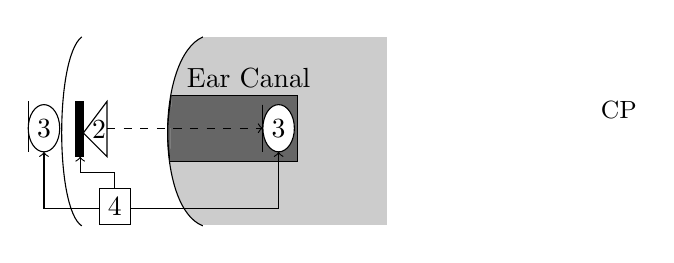
\begin{tikzpicture}
\draw [](-2.22,2.52) node (v1) {} .. controls (-2.56,2.26) and (-2.56,0.34) .. (-2.22,0.12) node (v2) {};

\draw [draw=black,fill=black!20](-0.68,2.52) node (v1) {} .. controls (-1.28,2.26) and (-1.28,0.34) .. (-0.68,0.12) node (v2) {};
\draw [white, fill=black!20](-0.68,2.52) -- (1.66,2.52) -- (1.66,0.12) -- (-0.68,0.12);


\draw [draw=black,fill=black!60](-1.08,1.78) node (v1) {} .. controls (-1.14,1.44) and (-1.14,1.24) .. (-1.1,0.94) node (v2) {};
\draw [draw=black,fill=black!60](-1.08,1.78) -- (0.52,1.78) -- (0.52,0.94) -- (-1.1,0.94);


\draw [draw=black,fill=white] (0.28,1.36) node (v3) {3} ellipse (0.2 and 0.3);
\draw [draw=black,fill=black](0.08,1.66) -- (0.08,1.06);

\draw [draw=black,fill=white] (-2.7,1.36) node (v3) {3} ellipse (0.2 and 0.3);
\draw [draw=black,fill=black](-2.9,1.7) -- (-2.9,1.06);


\draw [draw=black,fill=black] (-2.2,1.7) rectangle (-2.3,1);
\draw (-2.2,1.3) -- (-1.9,1.7) -- (-1.9,1) -- (-2.2,1.3);
\node at (-2,1.34) {2};


\draw[->,dashed] (-1.9,1.36) node[right=6.5,above]{\small{CP}}-- (0.08,1.36);
\draw  (-1.6,0.6) rectangle node{4}(-2,0.14);
\draw [->](-2,0.34) -- (-2.7,0.34) -- (-2.7,1.06);
\draw [->](-1.6,0.34) -- (0.28,0.34) -- (0.28,1.06);
\draw [->](-1.8,0.6) -- (-1.8,0.8) -- (-2.24,0.8) -- (-2.24,1);
\node at (-0.1,2) {Ear Canal};
\end{tikzpicture}
	\begin{itemize}
			\item Attenuate all kind of signals
			\item Process the signal upfront
			\item Delay of the system must be less than the propagation time
	\end{itemize}		
\end{frame}

\subsection{System delay}
\begin{frame}{Conversion delay}{Conversion delay}
	\begin{columns}
		\begin{column}{0.4\textwidth}
		\begin{itemize}
		\item Too much delay in converters
				\begin{itemize}
				\item $\Sigma \Delta$-converters
				\begin{itemize}
				\item Equivalent to 43 samples
				\end{itemize}								
				\end{itemize}
		\item TLV320AIC3204
				\begin{itemize}
				\item[\textcolor{MATLABred}{48 kHz}]= 900 $\mu S$ $\approx 31$ cm
				\item[\textcolor{MATLAByellow}{96 kHz}]= 450 $\mu S$ $\approx 15$ cm
				\item[\textcolor{MATLABpurple}{192 kHz}]= 225 $\mu S$ $\approx 8$ cm
				\end{itemize}	
				\item Mems 	microphone less delay	 
		\end{itemize}
		\end{column}
		\begin{column}{0.6\textwidth} 
		\begin{center}
		% This file was created by matlab2tikz.
%
%The latest updates can be retrieved from
%  http://www.mathworks.com/matlabcentral/fileexchange/22022-matlab2tikz-matlab2tikz
%where you can also make suggestions and rate matlab2tikz.
%
\definecolor{mycolor1}{rgb}{0.00000,0.44700,0.74100}%
\definecolor{mycolor2}{rgb}{0.85000,0.32500,0.09800}%
\definecolor{mycolor3}{rgb}{0.92900,0.69400,0.12500}%
\definecolor{mycolor4}{rgb}{0.49400,0.18400,0.55600}%
%
\begin{tikzpicture}

\begin{axis}[%
width=5in,
height=3in,
xmajorgrids,
xminorgrids,
ymajorgrids,
yminorgrids,
scale only axis,
xmin=-0.0001,
xmax=0.0012,
ymin=-0.6,
ymax=0.6,
ylabel={Voltage [V]},
xlabel={Time [S]},
axis background/.style={fill=white},
%legend style={legend cell align=left,align=left,draw=white!15!black}
]
\addplot [color=mycolor1,solid,thick]
  table[row sep=crcr]{%
-0.00010012	-0.5733\\
-0.00010012	-0.5733\\
-9.9069e-05	-0.5743\\
-9.6969e-05	-0.57464\\
-9.4869e-05	-0.57296\\
-9.4269e-05	-0.57263\\
-9.2169e-05	-0.5743\\
-9.2169e-05	-0.5743\\
-9.0519e-05	-0.57296\\
-8.8719e-05	-0.57296\\
-8.8119e-05	-0.57464\\
-8.6619e-05	-0.57464\\
-8.5719e-05	-0.57296\\
-8.4369e-05	-0.5733\\
-8.1969e-05	-0.57464\\
-8.1669e-05	-0.5743\\
-8.0619e-05	-0.57263\\
-7.8369e-05	-0.57363\\
-7.7619e-05	-0.57263\\
-7.5669e-05	-0.5743\\
-7.4169e-05	-0.57296\\
-7.3419e-05	-0.57263\\
-7.1619e-05	-0.57397\\
-7.1469e-05	-0.57397\\
-7.0719e-05	-0.57296\\
-6.8769e-05	-0.5733\\
-6.7569e-05	-0.57263\\
-6.5619e-05	-0.57397\\
-6.3969e-05	-0.57296\\
-6.3669e-05	-0.57296\\
-6.1119e-05	-0.57464\\
-6.0969e-05	-0.57464\\
-5.8869e-05	-0.57263\\
-5.7819e-05	-0.57296\\
-5.7369e-05	-0.5743\\
-5.5569e-05	-0.57263\\
-5.4519e-05	-0.57397\\
-5.3019e-05	-0.57263\\
-5.1969e-05	-0.57363\\
-5.0469e-05	-0.5733\\
-4.9419e-05	-0.57464\\
-4.8069e-05	-0.57397\\
-4.6419e-05	-0.57195\\
-4.5069e-05	-0.57229\\
-4.3719e-05	-0.5743\\
-4.2819e-05	-0.57296\\
-4.1919e-05	-0.57397\\
-3.8619e-05	-0.57464\\
-3.8019e-05	-0.5733\\
-3.7569e-05	-0.5743\\
-3.5769e-05	-0.57263\\
-3.4419e-05	-0.57296\\
-3.3819e-05	-0.5743\\
-3.2319e-05	-0.57263\\
-3.1869e-05	-0.57363\\
-2.8719e-05	-0.57229\\
-2.7369e-05	-0.57363\\
-2.7219e-05	-0.57363\\
-2.4819e-05	-0.57263\\
-2.4519e-05	-0.5733\\
-2.4369e-05	-0.57263\\
-2.1669e-05	-0.57229\\
-2.0919e-05	-0.57363\\
-1.8969e-05	-0.5733\\
-1.8369e-05	-0.5743\\
-1.6869e-05	-0.57397\\
-1.5219e-05	-0.57263\\
-1.3119e-05	-0.57263\\
-1.1919e-05	-0.5743\\
-9.8194e-06	-0.57464\\
-9.3694e-06	-0.5733\\
-8.7694e-06	-0.57397\\
-7.5694e-06	-0.57263\\
-6.2194e-06	-0.57263\\
-5.1694e-06	-0.57363\\
-3.2194e-06	-0.57195\\
-2.1694e-06	-0.57363\\
-9.6936e-07	-0.57397\\
1.4306e-06	0.38857\\
1.4306e-06	0.38857\\
3.3806e-06	0.4238\\
4.7306e-06	0.42212\\
5.0306e-06	0.42346\\
7.1306e-06	0.42313\\
8.7806e-06	0.42178\\
9.5306e-06	0.42178\\
1.0431e-05	0.42346\\
1.1781e-05	0.42212\\
1.2831e-05	0.42111\\
1.4331e-05	0.42111\\
1.5981e-05	0.42245\\
1.7331e-05	0.42111\\
1.7631e-05	0.42178\\
1.9731e-05	0.42078\\
2.0631e-05	0.42178\\
2.2131e-05	0.42145\\
2.3931e-05	0.42044\\
2.6031e-05	0.42212\\
2.6781e-05	0.42011\\
2.7981e-05	0.42044\\
2.9631e-05	0.42145\\
3.0081e-05	0.42145\\
3.0831e-05	0.42011\\
3.3081e-05	0.42178\\
3.4731e-05	0.42044\\
3.6231e-05	0.42145\\
3.7581e-05	0.41977\\
3.7731e-05	0.42011\\
3.9231e-05	0.42111\\
4.0431e-05	0.42078\\
4.1631e-05	0.41943\\
4.3581e-05	0.41977\\
4.4931e-05	0.41876\\
4.5531e-05	0.4191\\
4.6581e-05	0.42078\\
4.8231e-05	0.41977\\
4.8531e-05	0.42044\\
5.2281e-05	0.42078\\
5.3181e-05	0.41977\\
5.3481e-05	0.42044\\
5.3931e-05	0.41943\\
5.6181e-05	0.41977\\
5.7531e-05	0.42111\\
5.8731e-05	0.41977\\
5.9181e-05	0.42111\\
6.1131e-05	0.42044\\
6.2031e-05	0.41943\\
6.3831e-05	0.41943\\
6.4731e-05	0.42111\\
6.6681e-05	0.41943\\
6.7581e-05	0.42044\\
6.9831e-05	0.42078\\
7.0731e-05	0.41943\\
7.1781e-05	0.42044\\
7.3431e-05	0.4191\\
7.4481e-05	0.41943\\
7.4631e-05	0.42044\\
7.6731e-05	0.42044\\
7.8531e-05	0.4191\\
7.9431e-05	0.41943\\
8.1531e-05	0.42078\\
8.2281e-05	0.42078\\
8.4231e-05	0.41943\\
8.4531e-05	0.42011\\
8.5431e-05	0.4191\\
8.8881e-05	0.42044\\
8.9631e-05	0.4191\\
8.9781e-05	0.41943\\
9.0531e-05	0.42044\\
9.2481e-05	0.42011\\
9.3231e-05	0.4191\\
9.6081e-05	0.42044\\
9.7431e-05	0.41943\\
9.7581e-05	0.42011\\
9.8781e-05	0.41843\\
0.00010013	0.4191\\
0.00010118	0.42044\\
0.00010283	0.4191\\
0.00010358	0.42044\\
0.00010553	0.4191\\
0.00010598	0.42011\\
0.00010793	0.4191\\
0.00010838	0.42011\\
0.00011078	0.42011\\
0.00011183	0.4191\\
0.00011318	0.42011\\
0.00011573	0.4191\\
0.00011663	0.42011\\
0.00011798	0.41809\\
0.00011843	0.41843\\
0.00011948	0.41977\\
0.00012143	0.41876\\
0.00012188	0.42044\\
0.00012413	0.41843\\
0.00012623	0.42011\\
0.00012623	0.42011\\
0.00012803	0.4191\\
0.00012878	0.4191\\
0.00012908	0.42011\\
0.00013148	0.41943\\
0.00013253	0.42044\\
0.00013553	0.4191\\
0.00013643	0.42044\\
0.00013703	0.42044\\
0.00013853	0.41809\\
0.00013913	0.41876\\
0.00014093	0.42011\\
0.00014183	0.41977\\
0.00014213	0.41876\\
0.00014468	0.41876\\
0.00014663	0.41977\\
0.00014708	0.42011\\
0.00014753	0.4191\\
0.00014963	0.4191\\
0.00015113	0.42078\\
0.00015293	0.4191\\
0.00015473	0.42011\\
0.00015488	0.42044\\
0.00015698	0.4191\\
0.00015743	0.41977\\
0.00015953	0.41843\\
0.00015998	0.4191\\
0.00016148	0.41977\\
0.00016253	0.41977\\
0.00016448	0.41809\\
0.00016553	0.41977\\
0.00016763	0.41843\\
0.00016853	0.41843\\
0.00016943	0.42011\\
0.00017093	0.41843\\
0.00017153	0.41977\\
0.00017453	0.41843\\
0.00017528	0.42011\\
0.00017573	0.42044\\
0.00017768	0.41843\\
0.00017813	0.4191\\
0.00017888	0.42044\\
0.00018188	0.41876\\
0.00018233	0.42011\\
0.00018338	0.41876\\
0.00018473	0.42011\\
0.00018713	0.41843\\
0.00018818	0.41977\\
0.00018953	0.41876\\
0.00019058	0.42011\\
0.00019208	0.41977\\
0.00019388	0.41809\\
0.00019388	0.41809\\
0.00019598	0.41977\\
0.00019643	0.41977\\
0.00019868	0.41809\\
0.00019943	0.41843\\
0.00020048	0.41943\\
0.00020183	0.41876\\
0.00020198	0.41943\\
0.00020423	0.41943\\
0.00020498	0.42044\\
0.00020678	0.42011\\
0.00020708	0.4191\\
0.00021023	0.41977\\
0.00021203	0.41843\\
0.00021203	0.41843\\
0.00021383	0.41977\\
0.00021473	0.42011\\
0.00021593	0.41876\\
0.00021728	0.4191\\
0.00021923	0.41809\\
0.00021983	0.41843\\
0.00022088	0.41977\\
0.00022238	0.41876\\
0.00022358	0.41977\\
0.00022568	0.41977\\
0.00022613	0.41843\\
0.00022823	0.41843\\
0.00022958	0.42011\\
0.00023093	0.41876\\
0.00023258	0.42044\\
0.00023288	0.42044\\
0.00023468	0.4191\\
0.00023603	0.42011\\
0.00023738	0.41876\\
0.00023828	0.4191\\
0.00023903	0.41809\\
0.00024233	0.41977\\
0.00024293	0.41843\\
0.00024338	0.41876\\
0.00024473	0.41943\\
0.00024698	0.41843\\
0.00024803	0.41943\\
0.00024848	0.4191\\
0.00025058	0.42044\\
0.00025103	0.41943\\
0.00025298	0.41843\\
0.00025373	0.41876\\
0.00025418	0.41943\\
0.00025628	0.4191\\
0.00025643	0.41809\\
0.00025928	0.41843\\
0.00026138	0.41977\\
0.00026138	0.41977\\
0.00026333	0.41809\\
0.00026453	0.41843\\
0.00026513	0.42011\\
0.00026663	0.41977\\
0.00026708	0.41843\\
0.00026933	0.41977\\
0.00026978	0.41843\\
0.00027353	0.41943\\
0.00027443	0.41843\\
0.00027443	0.41843\\
0.00027518	0.41943\\
0.00027713	0.41843\\
0.00027728	0.41943\\
0.00027968	0.41843\\
0.00028088	0.41977\\
0.00028238	0.41809\\
0.00028478	0.4191\\
0.00028478	0.4191\\
0.00028673	0.41776\\
0.00028853	0.41776\\
0.00029003	0.42011\\
0.00029003	0.42011\\
0.00029078	0.41876\\
0.00029258	0.4191\\
0.00029288	0.41809\\
0.00029573	0.41943\\
0.00029708	0.41776\\
0.00029783	0.41843\\
0.00029858	0.41977\\
0.00030038	0.41977\\
0.00030278	0.41776\\
0.00030323	0.41742\\
0.00030458	0.41943\\
0.00030608	0.4191\\
0.00030623	0.41809\\
0.00030863	0.41943\\
0.00030938	0.41809\\
0.00031148	0.41943\\
0.00031283	0.41809\\
0.00031373	0.41943\\
0.00031553	0.41809\\
0.00031658	0.4191\\
0.00031793	0.41776\\
0.00031868	0.41843\\
0.00031973	0.41977\\
0.00032123	0.4191\\
0.00032153	0.41809\\
0.00032543	0.41943\\
0.00032633	0.41776\\
0.00032663	0.41843\\
0.00032783	0.4191\\
0.00032963	0.41809\\
0.00033128	0.4191\\
0.00033173	0.4191\\
0.00033263	0.41776\\
0.00033443	0.4191\\
0.00033653	0.41809\\
0.00033743	0.41776\\
0.00033863	0.4191\\
0.00033998	0.41776\\
0.00034133	0.4191\\
0.00034208	0.41876\\
0.00034253	0.41776\\
0.00034538	0.4191\\
0.00034643	0.41742\\
0.00034823	0.41776\\
0.00034988	0.4191\\
0.00035048	0.41809\\
0.00035108	0.41943\\
0.00035243	0.4191\\
0.00035363	0.41776\\
0.00035543	0.4191\\
0.00035618	0.41776\\
0.00035798	0.4191\\
0.00035828	0.41843\\
0.00036038	0.41943\\
0.00036128	0.41809\\
0.00036278	0.41876\\
0.00036458	0.41742\\
0.00036548	0.41843\\
0.00036578	0.41742\\
0.00036803	0.41776\\
0.00037028	0.41876\\
0.00037073	0.41843\\
0.00037283	0.41742\\
0.00037508	0.41876\\
0.00037583	0.41709\\
0.00037583	0.41709\\
0.00037808	0.41876\\
0.00037883	0.41776\\
0.00038063	0.4191\\
0.00038183	0.41843\\
0.00038258	0.41742\\
0.00038393	0.41843\\
0.00038513	0.41742\\
0.00038648	0.41876\\
0.00038873	0.41742\\
0.00038888	0.41742\\
0.00038993	0.4191\\
0.00039158	0.41742\\
0.00039368	0.41843\\
0.00039443	0.41742\\
0.00039578	0.41843\\
0.00039728	0.41742\\
0.00039923	0.41843\\
0.00039953	0.41776\\
0.00039968	0.41876\\
0.00040178	0.41776\\
0.00040448	0.41876\\
0.00040538	0.41776\\
0.00040688	0.4191\\
0.00040718	0.41876\\
0.00040793	0.41776\\
0.00041153	0.4191\\
0.00041213	0.41742\\
0.00041228	0.41742\\
0.00041288	0.41876\\
0.00041528	0.41843\\
0.00041588	0.41742\\
0.00041783	0.41709\\
0.00041978	0.41843\\
0.00042008	0.41809\\
0.00042218	0.41675\\
0.00042278	0.41675\\
0.00042398	0.41809\\
0.00042638	0.41675\\
0.00042698	0.41843\\
0.00042833	0.41642\\
0.00042938	0.4191\\
0.00043103	0.41843\\
0.00043268	0.41709\\
0.00043298	0.41709\\
0.00043508	0.41843\\
0.00043568	0.41843\\
0.00043748	0.41642\\
0.00043853	0.41675\\
0.00043928	0.41776\\
0.00044078	0.41709\\
0.00044123	0.41843\\
0.00044393	0.41675\\
0.00044573	0.41843\\
0.00044603	0.41843\\
0.00044693	0.41709\\
0.00044888	0.41742\\
0.00044948	0.41843\\
0.00045143	0.41709\\
0.00045203	0.41843\\
0.00045533	0.41809\\
0.00045623	0.41709\\
0.00045698	0.41709\\
0.00045713	0.41809\\
0.00045998	0.41809\\
0.00046133	0.41642\\
0.00046178	0.41642\\
0.00046253	0.41843\\
0.00046463	0.41776\\
0.00046583	0.41675\\
0.00046688	0.41709\\
0.00046898	0.41843\\
0.00046958	0.41776\\
0.00047063	0.41876\\
0.00047213	0.41876\\
0.00047348	0.41709\\
0.00047498	0.41876\\
0.00047573	0.41742\\
0.00047768	0.41809\\
0.00047933	0.41709\\
0.00048023	0.41809\\
0.00048248	0.41574\\
0.00048248	0.41574\\
0.00048413	0.41809\\
0.00048518	0.41776\\
0.00048623	0.41675\\
0.00048863	0.41809\\
0.00048983	0.41675\\
0.00049028	0.41809\\
0.00049118	0.41709\\
0.00049523	0.41709\\
0.00049538	0.41843\\
0.00049598	0.41876\\
0.00049763	0.41709\\
0.00049808	0.41776\\
0.00049853	0.41709\\
0.00050123	0.41876\\
0.00050213	0.41709\\
0.00050363	0.41709\\
0.00050498	0.41809\\
0.00050693	0.41675\\
0.00050708	0.41809\\
0.00050873	0.41809\\
0.00051113	0.41642\\
0.00051173	0.41608\\
0.00051308	0.41742\\
0.00051368	0.41675\\
0.00051488	0.41809\\
0.00051743	0.41742\\
0.00051833	0.41608\\
0.00051893	0.41675\\
0.00052028	0.41742\\
0.00052223	0.41843\\
0.00052328	0.41709\\
0.00052403	0.41809\\
0.00052643	0.41675\\
0.00052688	0.41709\\
0.00052823	0.41809\\
0.00052958	0.41742\\
0.00053168	0.41843\\
0.00053273	0.41709\\
0.00053453	0.41843\\
0.00053453	0.41843\\
0.00053528	0.41642\\
0.00053843	0.41608\\
0.00053948	0.41742\\
0.00053963	0.41675\\
0.00054158	0.41776\\
0.00054293	0.41608\\
0.00054428	0.41809\\
0.00054503	0.41608\\
0.00054698	0.41776\\
0.00054803	0.41776\\
0.00054878	0.41642\\
0.00055103	0.41776\\
0.00055193	0.41675\\
0.00055268	0.41675\\
0.00055403	0.41809\\
0.00055523	0.41776\\
0.00055688	0.41675\\
0.00055943	0.41574\\
0.00056048	0.41742\\
0.00056048	0.41742\\
0.00056243	0.41574\\
0.00056438	0.41642\\
0.00056573	0.41776\\
0.00056573	0.41776\\
0.00056783	0.41642\\
0.00056828	0.41675\\
0.00056858	0.41776\\
0.00057098	0.41675\\
0.00057158	0.41809\\
0.00057353	0.41742\\
0.00057443	0.41642\\
0.00057713	0.41709\\
0.00057833	0.41608\\
0.00057863	0.41642\\
0.00058118	0.41776\\
0.00058163	0.41742\\
0.00058358	0.41642\\
0.00058448	0.41776\\
0.00058598	0.41642\\
0.00058688	0.41574\\
0.00058823	0.41709\\
0.00059033	0.41675\\
0.00059138	0.41574\\
0.00059213	0.41574\\
0.00059378	0.41742\\
0.00059423	0.41709\\
0.00059483	0.41574\\
0.00059693	0.41574\\
0.00059783	0.41709\\
0.00059948	0.41574\\
0.00060143	0.41675\\
0.00060203	0.41608\\
0.00060368	0.41742\\
0.00060488	0.41642\\
0.00060563	0.41742\\
0.00060728	0.41642\\
0.00060893	0.41742\\
0.00061043	0.41709\\
0.00061133	0.41608\\
0.00061283	0.41742\\
0.00061478	0.41574\\
0.00061583	0.41709\\
0.00061658	0.41507\\
0.00061763	0.41574\\
0.00061853	0.41742\\
0.00062033	0.41675\\
0.00062123	0.41541\\
0.00062333	0.41574\\
0.00062423	0.41742\\
0.00062573	0.41709\\
0.00062813	0.41574\\
0.00062813	0.41574\\
0.00063053	0.41709\\
0.00063083	0.41675\\
0.00063173	0.41776\\
0.00063323	0.41742\\
0.00063383	0.41608\\
0.00063683	0.41675\\
0.00063788	0.41541\\
0.00063848	0.41608\\
0.00063923	0.41541\\
0.00064178	0.41541\\
0.00064223	0.41642\\
0.00064373	0.41574\\
0.00064448	0.41709\\
0.00064643	0.41709\\
0.00064778	0.41507\\
0.00064898	0.41675\\
0.00064988	0.41541\\
0.00065243	0.41742\\
0.00065348	0.41574\\
0.00065408	0.41608\\
0.00065543	0.41709\\
0.00065663	0.41675\\
0.00065738	0.41574\\
0.00066008	0.41541\\
0.00066173	0.41675\\
0.00066248	0.41642\\
0.00066353	0.41541\\
0.00066458	0.41541\\
0.00066473	0.41675\\
0.00066863	0.41709\\
0.00066938	0.41541\\
0.00066998	0.41574\\
0.00067178	0.41742\\
0.00067253	0.41776\\
0.00067478	0.41608\\
0.00067523	0.41541\\
0.00067658	0.41675\\
0.00067748	0.41642\\
0.00067958	0.41474\\
0.00068003	0.41541\\
0.00068093	0.41642\\
0.00068333	0.41642\\
0.00068438	0.41507\\
0.00068648	0.41507\\
0.00068723	0.41709\\
0.00068798	0.41709\\
0.00069023	0.41541\\
0.00069128	0.41541\\
0.00069293	0.41709\\
0.00069323	0.41608\\
0.00069368	0.41709\\
0.00069563	0.41642\\
0.00069698	0.41507\\
0.00069953	0.41507\\
0.00070088	0.41608\\
0.00070088	0.41608\\
0.00070328	0.41507\\
0.00070418	0.4144\\
0.00070553	0.41608\\
0.00070643	0.41474\\
0.00070793	0.41608\\
0.00070928	0.41608\\
0.00070958	0.41507\\
0.00071183	0.41541\\
0.00071198	0.41642\\
0.00071453	0.41541\\
0.00071498	0.41642\\
0.00071678	0.41541\\
0.00071858	0.41675\\
0.00071903	0.41675\\
0.00072068	0.41541\\
0.00072173	0.41608\\
0.00072308	0.41507\\
0.00072443	0.41608\\
0.00072638	0.41507\\
0.00072728	0.41642\\
0.00072848	0.41541\\
0.00072983	0.41608\\
0.00073028	0.41541\\
0.00073313	0.41608\\
0.00073418	0.41474\\
0.00073463	0.41541\\
0.00073523	0.41474\\
0.00073778	0.41574\\
0.00073808	0.41507\\
0.00074063	0.41642\\
0.00074168	0.4144\\
0.00074258	0.41507\\
0.00074273	0.41574\\
0.00074633	0.41608\\
0.00074663	0.41507\\
0.00074813	0.41474\\
0.00074858	0.41608\\
0.00075038	0.41507\\
0.00075263	0.41642\\
0.00075308	0.41574\\
0.00075413	0.4144\\
0.00075698	0.41574\\
0.00075713	0.41474\\
0.00075818	0.41541\\
0.00076028	0.4144\\
0.00076088	0.41474\\
0.00076178	0.41574\\
0.00076358	0.4144\\
0.00076448	0.41574\\
0.00076628	0.41507\\
0.00076658	0.41608\\
0.00076853	0.41574\\
0.00076988	0.41474\\
0.00077138	0.4144\\
0.00077183	0.41574\\
0.00077378	0.41541\\
0.00077453	0.4144\\
0.00077648	0.41474\\
0.00077858	0.41574\\
0.00077888	0.41541\\
0.00078023	0.4144\\
0.00078188	0.41474\\
0.00078203	0.41574\\
0.00078428	0.41507\\
0.00078623	0.41373\\
0.00078698	0.4144\\
0.00078803	0.41574\\
0.00078938	0.4144\\
0.00079148	0.41574\\
0.00079208	0.41608\\
0.00079403	0.41474\\
0.00079448	0.41507\\
0.00079508	0.41407\\
0.00079763	0.41373\\
0.00079853	0.41507\\
0.00079988	0.4144\\
0.00080198	0.41608\\
0.00080258	0.41574\\
0.00080378	0.41407\\
0.00080498	0.41541\\
0.00080738	0.4144\\
0.00080783	0.4144\\
0.00080813	0.41541\\
0.00081008	0.41507\\
0.00081128	0.41407\\
0.00081293	0.41507\\
0.00081398	0.4134\\
0.00081548	0.41507\\
0.00081683	0.41373\\
0.00081863	0.41373\\
0.00082013	0.41507\\
0.00082148	0.41407\\
0.00082223	0.41541\\
0.00082403	0.4134\\
0.00082538	0.41474\\
0.00082598	0.41407\\
0.00082658	0.41507\\
0.00082913	0.41407\\
0.00083048	0.41574\\
0.00083093	0.41474\\
0.00083198	0.41574\\
0.00083363	0.41474\\
0.00083438	0.41541\\
0.00083678	0.41608\\
0.00083798	0.41474\\
0.00083888	0.41541\\
0.00083963	0.41407\\
0.00084263	0.41541\\
0.00084293	0.41407\\
0.00084473	0.41373\\
0.00084638	0.41507\\
0.00084728	0.41407\\
0.00084743	0.41507\\
0.00084938	0.41574\\
0.00085103	0.41407\\
0.00085178	0.41407\\
0.00085238	0.41507\\
0.00085463	0.41474\\
0.00085658	0.41306\\
0.00085733	0.41306\\
0.00085823	0.41407\\
0.00085988	0.41373\\
0.00086168	0.41541\\
0.00086333	0.41541\\
0.00086423	0.41407\\
0.00086513	0.41407\\
0.00086603	0.41574\\
0.00086768	0.41373\\
0.00086978	0.41474\\
0.00086993	0.41373\\
0.00087128	0.41541\\
0.00087263	0.41474\\
0.00087293	0.41373\\
0.00087578	0.4144\\
0.00087728	0.4134\\
0.00087833	0.41306\\
0.00087893	0.4144\\
0.00088058	0.41373\\
0.00088283	0.41507\\
0.00088388	0.41474\\
0.00088523	0.41373\\
0.00088553	0.41407\\
0.00088778	0.41541\\
0.00088823	0.41574\\
0.00088988	0.41373\\
0.00089108	0.41507\\
0.00089333	0.41407\\
0.00089363	0.41474\\
0.00089558	0.41306\\
0.00089588	0.41373\\
0.00089648	0.41507\\
0.00089903	0.41474\\
0.00090053	0.4134\\
0.00090113	0.41474\\
0.00090128	0.41407\\
0.00090368	0.4144\\
0.00090473	0.41272\\
0.00090668	0.41373\\
0.00090788	0.41507\\
0.00090968	0.41306\\
0.00091118	0.41541\\
0.00091163	0.41541\\
0.00091403	0.41306\\
0.00091463	0.4144\\
0.00091553	0.41306\\
0.00091748	0.41373\\
0.00091763	0.4144\\
0.00092003	0.41474\\
0.00092048	0.4134\\
0.00092213	0.4144\\
0.00092258	0.4134\\
0.00092453	0.4134\\
0.00092618	0.41507\\
0.00092708	0.4144\\
0.00092888	0.4134\\
0.00093038	0.4134\\
0.00093098	0.41474\\
0.00093248	0.41407\\
0.00093443	0.41239\\
0.00093638	0.41239\\
0.00093758	0.4144\\
0.00093758	0.4144\\
0.00093848	0.41272\\
0.00094058	0.41306\\
0.00094178	0.4144\\
0.00094268	0.41306\\
0.00094283	0.4144\\
0.00094538	0.4144\\
0.00094598	0.41373\\
0.00094808	0.4134\\
0.00094898	0.41474\\
0.00095213	0.41474\\
0.00095258	0.41306\\
0.00095318	0.41373\\
0.00095408	0.41272\\
0.00095678	0.41272\\
0.00095813	0.41407\\
0.00095888	0.41507\\
0.00096053	0.41239\\
0.00096098	0.41306\\
0.00096248	0.41407\\
0.00096398	0.41407\\
0.00096473	0.41306\\
0.00096608	0.4134\\
0.00096743	0.41507\\
0.00096953	0.41507\\
0.00097058	0.4134\\
0.00097148	0.4144\\
0.00097283	0.41306\\
0.00097493	0.4134\\
0.00097658	0.41474\\
0.00097688	0.41474\\
0.00097868	0.41272\\
0.00097958	0.41239\\
0.00098093	0.41373\\
0.00098183	0.41407\\
0.00098348	0.41306\\
0.00098558	0.41306\\
0.00098648	0.4144\\
0.00098723	0.4134\\
0.00098828	0.4144\\
0.00098993	0.41306\\
0.00099173	0.41474\\
0.00099218	0.4144\\
0.00099368	0.41272\\
0.00099473	0.41306\\
0.00099713	0.4144\\
0.00099833	0.41407\\
0.00099953	0.41239\\
0.0010003	0.41239\\
0.0010013	0.41373\\
0.0010028	0.4144\\
0.0010045	0.41239\\
0.0010051	0.41272\\
0.0010061	0.41407\\
0.0010081	0.41407\\
0.0010099	0.41205\\
0.0010105	0.4134\\
0.0010115	0.41272\\
0.0010132	0.41239\\
0.0010142	0.41373\\
0.0010162	0.41306\\
0.0010181	0.4144\\
0.0010181	0.4144\\
0.0010184	0.41306\\
0.0010208	0.41407\\
0.0010226	0.41205\\
0.0010252	0.41239\\
0.0010259	0.41407\\
0.0010285	0.4134\\
};
\addlegendentry{2 Hz Step};

\addplot [color=mycolor2,solid,thick]
  table[row sep=crcr]{%
-0.00010012	-0.0041845\\
-9.9819e-05	0.033263\\
-9.7869e-05	-0.027255\\
-9.7119e-05	0.034266\\
-9.6519e-05	-0.054672\\
-9.3219e-05	0.0055117\\
-9.2169e-05	-0.032604\\
-9.0369e-05	-0.086769\\
-8.9619e-05	0.051987\\
-8.9619e-05	0.051987\\
-8.7069e-05	-0.075401\\
-8.7069e-05	-0.075401\\
-8.6469e-05	0.067701\\
-8.3919e-05	0.071045\\
-8.3169e-05	-0.092119\\
-8.1819e-05	-0.041632\\
-8.1219e-05	0.025238\\
-7.7169e-05	0.012867\\
-7.6569e-05	-0.021905\\
-7.5669e-05	0.033932\\
-7.4919e-05	-0.050994\\
-7.3869e-05	0.023232\\
-7.2669e-05	-0.040295\\
-7.1019e-05	-0.043972\\
-7.0119e-05	0.03226\\
-6.7119e-05	0.021895\\
-6.6369e-05	-0.041632\\
-6.4419e-05	0.062351\\
-6.3669e-05	-0.080082\\
-6.2769e-05	0.029919\\
-6.1269e-05	-0.092453\\
-6.0519e-05	0.10247\\
-5.9769e-05	-0.078411\\
-5.6469e-05	-0.05835\\
-5.5869e-05	0.045968\\
-5.4369e-05	0.058005\\
-5.3469e-05	-0.070386\\
-5.1519e-05	0.04764\\
-5.0919e-05	-0.074064\\
-5.0019e-05	0.068035\\
-4.9119e-05	-0.073061\\
-4.8069e-05	0.0346\\
-4.7169e-05	-0.031936\\
-4.3869e-05	0.025573\\
-4.2969e-05	-0.055006\\
-4.2819e-05	-0.040963\\
-4.2219e-05	0.046637\\
-3.8619e-05	-0.046647\\
-3.7869e-05	0.038278\\
-3.6969e-05	-0.041966\\
-3.6069e-05	0.022229\\
-3.3519e-05	0.087428\\
-3.2769e-05	-0.092453\\
-3.2469e-05	-0.042301\\
-3.1869e-05	0.036941\\
-2.7819e-05	0.04229\\
-2.7219e-05	-0.066374\\
-2.7069e-05	-0.070721\\
-2.6469e-05	0.059677\\
-2.2869e-05	-0.079414\\
-2.2119e-05	0.067367\\
-2.1969e-05	0.062351\\
-2.1069e-05	-0.037285\\
-1.8369e-05	0.050983\\
-1.7619e-05	-0.063365\\
-1.6719e-05	0.045634\\
-1.4169e-05	-0.045644\\
-1.4019e-05	-0.047316\\
-1.1919e-05	0.046303\\
-1.0569e-05	0.066698\\
-9.9694e-06	-0.097469\\
-8.0194e-06	0.077397\\
-7.2694e-06	-0.10349\\
-5.9194e-06	-0.06838\\
-5.3194e-06	0.049646\\
-3.8194e-06	0.015877\\
-1.8694e-06	-0.044307\\
-9.6936e-07	0.028916\\
1.1306e-06	-0.035279\\
1.8806e-06	0.028248\\
2.7806e-06	-0.041632\\
5.4806e-06	-0.093791\\
6.2306e-06	0.082413\\
8.6306e-06	-0.091785\\
9.2306e-06	0.072048\\
9.5306e-06	0.11418\\
1.0281e-05	-0.10382\\
1.3431e-05	0.031257\\
1.4181e-05	-0.034611\\
1.6281e-05	0.031925\\
1.7031e-05	-0.040629\\
1.8531e-05	-0.062362\\
1.9281e-05	0.073719\\
2.0031e-05	-0.079414\\
2.0781e-05	0.035269\\
2.2281e-05	0.027913\\
2.3331e-05	-0.028592\\
2.6031e-05	-0.02692\\
2.6781e-05	0.022229\\
2.8581e-05	0.019554\\
2.9481e-05	-0.050325\\
3.0231e-05	0.036606\\
3.2631e-05	-0.060021\\
3.2781e-05	-0.066708\\
3.3531e-05	0.054996\\
3.5631e-05	-0.036617\\
3.7581e-05	0.034266\\
3.9381e-05	0.058339\\
4.0131e-05	-0.059018\\
4.1331e-05	-0.078411\\
4.2081e-05	0.058339\\
4.3431e-05	0.057336\\
4.4181e-05	-0.069383\\
4.5981e-05	0.028582\\
4.6581e-05	-0.055675\\
4.8831e-05	-0.067043\\
4.9581e-05	0.077397\\
5.1681e-05	-0.023243\\
5.3331e-05	0.02691\\
5.4231e-05	-0.051662\\
5.6031e-05	0.042959\\
5.7981e-05	-0.12856\\
5.8581e-05	0.085087\\
5.8731e-05	0.097793\\
6.0681e-05	-0.066708\\
6.1431e-05	0.081075\\
6.2181e-05	-0.08142\\
6.4431e-05	0.095452\\
6.5181e-05	-0.090447\\
6.7131e-05	0.03995\\
6.7731e-05	-0.05534\\
7.0881e-05	-0.065037\\
7.1631e-05	0.047974\\
7.1631e-05	0.047974\\
7.3731e-05	-0.070386\\
7.4481e-05	0.086759\\
7.5231e-05	-0.10583\\
7.7181e-05	0.034935\\
7.7781e-05	-0.06069\\
8.1231e-05	-0.054337\\
8.1981e-05	0.043628\\
8.3931e-05	0.048977\\
8.4531e-05	-0.067711\\
8.6031e-05	-0.080751\\
8.6631e-05	0.06302\\
8.8881e-05	-0.069383\\
8.9481e-05	0.063355\\
9.0231e-05	-0.072058\\
9.0831e-05	0.04764\\
9.2931e-05	-0.063699\\
9.3681e-05	0.053324\\
9.5181e-05	0.028248\\
9.5931e-05	-0.037954\\
9.9081e-05	0.036941\\
9.9681e-05	-0.039626\\
0.00010043	0.039616\\
0.00010103	-0.062362\\
0.00010433	0.042959\\
0.00010508	-0.070052\\
0.00010643	-0.080082\\
0.00010718	0.071379\\
0.00010793	-0.077408\\
0.00010853	0.051652\\
0.00011183	-0.085432\\
0.00011243	0.075391\\
0.00011318	-0.078411\\
0.00011543	0.046971\\
0.00011753	-0.062362\\
0.00011828	0.069373\\
0.00011918	-0.077742\\
0.00012008	0.066698\\
0.00012218	-0.066708\\
0.00012293	0.057336\\
0.00012368	-0.054003\\
0.00012428	0.035269\\
0.00012788	-0.067043\\
0.00012863	0.059677\\
0.00012938	-0.064033\\
0.00013133	0.067701\\
0.00013208	-0.082088\\
0.00013403	0.10649\\
0.00013403	0.10649\\
0.00013478	-0.11285\\
0.00013808	0.041956\\
0.00013883	-0.073395\\
0.00013958	0.042625\\
0.00014018	-0.043304\\
0.00014303	0.034935\\
0.00014378	-0.069383\\
0.00014453	0.043293\\
0.00014543	-0.02993\\
0.00014753	0.024235\\
0.00014933	-0.032939\\
0.00014993	0.055664\\
0.00015068	-0.06838\\
0.00015323	-0.057346\\
0.00015383	0.0453\\
0.00015653	0.046971\\
0.00015713	-0.060021\\
0.00015848	-0.077073\\
0.00015923	0.086759\\
0.00015998	-0.074064\\
0.00016058	0.024235\\
0.00016388	-0.059687\\
0.00016493	0.041622\\
0.00016583	-0.082757\\
0.00016658	0.060011\\
0.00016943	0.054327\\
0.00017003	-0.070052\\
0.00017078	0.070376\\
0.00017168	-0.075736\\
0.00017438	0.077397\\
0.00017513	-0.10549\\
0.00017573	0.085756\\
0.00017648	-0.070052\\
0.00017993	0.053658\\
0.00018068	-0.061693\\
0.00018248	0.052655\\
0.00018308	-0.063365\\
0.00018368	0.055664\\
0.00018563	-0.082423\\
0.00018638	0.060345\\
0.00018863	-0.061359\\
0.00018863	-0.061359\\
0.00018938	0.041622\\
0.00019148	-0.056009\\
0.00019223	0.05299\\
0.00019538	-0.086101\\
0.00019613	0.077063\\
0.00019748	0.0891\\
0.00019808	-0.099809\\
0.00019958	-0.10583\\
0.00020033	0.067701\\
0.00020273	-0.064702\\
0.00020363	0.06837\\
0.00020438	-0.061693\\
0.00020648	0.052321\\
0.00020828	0.069373\\
0.00020903	-0.075736\\
0.00020978	0.086425\\
0.00021053	-0.10148\\
0.00021263	0.061683\\
0.00021338	-0.070386\\
0.00021458	0.0095239\\
0.00021503	-0.022908\\
0.00021923	0.064692\\
0.00021983	-0.062362\\
0.00022043	0.034266\\
0.00022238	-0.065371\\
0.00022298	0.062351\\
0.00022373	-0.068714\\
0.00022703	-0.078411\\
0.00022763	0.078066\\
0.00022778	0.084084\\
0.00022853	-0.077073\\
0.00023063	0.024235\\
0.00023138	-0.038623\\
0.00023438	0.052655\\
0.00023513	-0.081085\\
0.00023543	-0.03762\\
0.00023798	0.067032\\
0.00023888	-0.085766\\
0.00024068	0.095452\\
0.00024068	0.095452\\
0.00024143	-0.10115\\
0.00024323	-0.043638\\
0.00024488	0.027245\\
0.00024773	0.064692\\
0.00024848	-0.087104\\
0.00024848	-0.087104\\
0.00024908	0.080072\\
0.00025208	0.042959\\
0.00025283	-0.057346\\
0.00025478	0.041622\\
0.00025553	-0.068046\\
0.00025628	0.041622\\
0.00025688	-0.033607\\
0.00026063	-0.061693\\
0.00026123	0.06837\\
0.00026138	0.056333\\
0.00026318	-0.055675\\
0.00026558	-0.047316\\
0.00026633	0.030254\\
0.00026828	0.053993\\
0.00026903	-0.057012\\
0.00026918	-0.052331\\
0.00027128	0.037609\\
0.00027203	-0.04765\\
0.00027293	0.02457\\
0.00027638	0.050315\\
0.00027698	-0.048653\\
0.00027713	-0.064033\\
0.00027788	0.023567\\
0.00028118	-0.042969\\
0.00028193	0.0346\\
0.00028298	-0.047316\\
0.00028373	0.026241\\
0.00028628	0.025238\\
0.00028718	-0.060356\\
0.00028898	0.072048\\
0.00028973	-0.1299\\
0.00029003	-0.056009\\
0.00029048	0.06837\\
0.00029288	0.048309\\
0.00029363	-0.062696\\
0.00029678	0.045968\\
0.00029753	-0.057012\\
0.00029813	0.041622\\
0.00030008	-0.064702\\
0.00030038	-0.02993\\
0.00030083	0.040953\\
0.00030428	0.036606\\
0.00030503	-0.041298\\
0.00030653	-0.046647\\
0.00030728	0.04764\\
0.00030968	-0.043972\\
0.00031058	0.036606\\
0.00031088	0.020557\\
0.00031178	-0.035279\\
0.00031403	0.037275\\
0.00031478	-0.049656\\
0.00031688	0.01688\\
0.00031763	-0.032604\\
0.00032033	0.015877\\
0.00032108	-0.036951\\
0.00032183	0.062017\\
0.00032258	-0.088776\\
0.00032393	-0.048653\\
0.00032453	0.032929\\
0.00032813	-0.031936\\
0.00032888	0.082078\\
0.00032903	0.052655\\
0.00032963	-0.10282\\
0.00033353	-0.072392\\
0.00033428	0.070376\\
0.00033428	0.070376\\
0.00033503	-0.063365\\
0.00033683	-0.030933\\
0.00033878	0.026241\\
0.00034118	-0.071389\\
0.00034178	0.078735\\
0.00034208	0.050983\\
0.00034268	-0.078745\\
0.00034673	-0.033942\\
0.00034718	0.01922\\
0.00034808	-0.05534\\
0.00034883	0.04229\\
0.00035168	0.027913\\
0.00035243	-0.034611\\
0.00035243	-0.034611\\
0.00035318	0.021895\\
0.00035543	0.043293\\
0.00035618	-0.045644\\
0.00035903	-0.030264\\
0.00035978	0.027579\\
0.00036143	0.055664\\
0.00036218	-0.069383\\
0.00036308	0.054327\\
0.00036398	-0.06303\\
0.00036728	0.028248\\
0.00036803	-0.071389\\
0.00036878	0.085087\\
0.00036953	-0.088441\\
0.00037268	-0.064033\\
0.00037328	0.064358\\
0.00037343	0.072382\\
0.00037418	-0.085098\\
0.00037628	0.059008\\
0.00037703	-0.073061\\
0.00037853	-0.038623\\
0.00038063	0.027245\\
0.00038288	-0.051662\\
0.00038363	0.04998\\
0.00038363	0.04998\\
0.00038588	-0.065705\\
0.00038648	0.066029\\
0.00038723	-0.068714\\
0.00039083	0.046971\\
0.00039143	-0.046982\\
0.00039293	-0.064033\\
0.00039368	0.053658\\
0.00039578	0.049312\\
0.00039653	-0.094125\\
0.00039668	-0.091116\\
0.00039923	0.066698\\
0.00039938	0.06837\\
0.00040013	-0.05534\\
0.00040388	-0.038957\\
0.00040448	0.025907\\
0.00040463	0.027579\\
0.00040538	-0.03227\\
0.00040838	-0.03996\\
0.00040913	0.042625\\
0.00041123	0.03995\\
0.00041213	-0.048653\\
0.00041228	-0.038623\\
0.00041288	0.040284\\
0.00041633	-0.044307\\
0.00041708	0.059677\\
0.00041783	-0.067711\\
0.00041843	0.04764\\
0.00042158	0.049646\\
0.00042233	-0.06069\\
0.00042323	0.042959\\
0.00042398	-0.045978\\
0.00042713	0.052655\\
0.00042773	-0.08142\\
0.00042788	-0.078411\\
0.00042848	0.074722\\
0.00043058	-0.077742\\
0.00043133	0.025573\\
0.00043373	-0.04531\\
0.00043553	0.0346\\
0.00043568	0.034266\\
0.00043643	-0.037285\\
0.00043883	-0.040295\\
0.00043958	0.032929\\
0.00044213	0.041956\\
0.00044288	-0.040963\\
0.00044363	0.016545\\
0.00044453	-0.024914\\
0.00044648	-0.030933\\
0.00044723	0.011864\\
0.00044888	0.025907\\
0.00044978	-0.04531\\
0.00045128	-0.036617\\
0.00045203	0.025573\\
0.00045548	0.061348\\
0.00045623	-0.054672\\
0.00045803	0.040284\\
0.00045878	-0.071055\\
0.00045953	0.057002\\
0.00046013	-0.053669\\
0.00046313	-0.078076\\
0.00046388	0.072048\\
0.00046463	-0.058684\\
0.00046658	0.051652\\
0.00046748	-0.046982\\
0.00046838	0.033932\\
0.00046943	-0.042301\\
0.00047003	0.041287\\
0.00047393	-0.03996\\
0.00047468	0.056667\\
0.00047543	-0.086435\\
0.00047618	0.057336\\
0.00047843	-0.098472\\
0.00047918	0.062351\\
0.00048113	0.032594\\
0.00048188	-0.046982\\
0.00048263	0.025238\\
0.00048338	-0.028927\\
0.00048683	0.023901\\
0.00048773	-0.050659\\
0.00048773	-0.050659\\
0.00049028	0.038612\\
0.00049118	-0.087104\\
0.00049193	0.048977\\
0.00049373	0.04229\\
0.00049448	-0.059687\\
0.00049688	-0.067043\\
0.00049763	0.04764\\
0.00049838	-0.049656\\
0.00049913	0.050315\\
0.00050168	-0.026252\\
0.00050273	0.026576\\
0.00050528	-0.072058\\
0.00050588	0.062017\\
0.00050603	0.079738\\
0.00050693	-0.10081\\
0.00051023	0.089768\\
0.00051083	-0.091116\\
0.00051158	0.057002\\
0.00051218	-0.06303\\
0.00051428	0.04229\\
0.00051503	-0.060021\\
0.00051653	-0.03762\\
0.00051728	0.012533\\
0.00051983	0.012533\\
0.00052133	-0.032939\\
0.00052208	0.088431\\
0.00052298	-0.05835\\
0.00052583	0.079738\\
0.00052658	-0.069049\\
0.00052673	-0.064033\\
0.00052733	0.048643\\
0.00052928	-0.060356\\
0.00053003	0.049646\\
0.00053333	0.087428\\
0.00053408	-0.11251\\
0.00053483	0.090771\\
0.00053618	-0.048319\\
0.00053873	0.11518\\
0.00053963	-0.11151\\
0.00053963	-0.11151\\
0.00054038	0.073051\\
0.00054308	0.061683\\
0.00054383	-0.078411\\
0.00054578	-0.11084\\
0.00054653	0.10247\\
0.00054878	-0.06303\\
0.00054953	0.079403\\
0.00055043	-0.062362\\
0.00055133	0.016211\\
0.00055343	0.0346\\
0.00055418	-0.039626\\
0.00055598	0.0055117\\
0.00055793	-0.023911\\
0.00055958	-0.043638\\
0.00056018	0.032594\\
0.00056108	-0.034945\\
0.00056303	0.017548\\
0.00056333	0.034266\\
0.00056408	-0.054337\\
0.00056708	-0.053334\\
0.00056783	0.056667\\
0.00056963	0.012533\\
0.00057038	-0.042969\\
0.00057128	0.04764\\
0.00057203	-0.064033\\
0.00057488	0.031925\\
0.00057578	-0.052666\\
0.00057758	0.041287\\
0.00057848	-0.085766\\
0.00057863	-0.071389\\
0.00057923	0.065361\\
0.00058148	-0.066374\\
0.00058223	0.057002\\
0.00058508	0.066698\\
0.00058598	-0.08376\\
0.00058658	0.054327\\
0.00058853	-0.077073\\
0.00058928	0.077397\\
0.00059003	-0.07373\\
0.00059288	-0.06069\\
0.00059363	0.03995\\
0.00059603	-0.04531\\
0.00059678	0.046637\\
0.00059753	-0.063699\\
0.00059843	0.048643\\
0.00060098	0.015877\\
0.00060173	-0.072727\\
0.00060263	0.09144\\
0.00060338	-0.11218\\
0.00060488	-0.075067\\
0.00060668	0.060345\\
0.00060743	-0.074398\\
0.00060818	0.043293\\
0.00061058	-0.031936\\
0.00061253	0.03995\\
0.00061328	-0.084763\\
0.00061403	0.070042\\
0.00061613	-0.058684\\
0.00061673	0.059008\\
0.00061943	0.056333\\
0.00062003	-0.057346\\
0.00062138	-0.044641\\
0.00062228	0.044296\\
0.00062333	-0.047316\\
0.00062423	0.028916\\
0.00062588	0.039281\\
0.00062663	-0.046647\\
0.00062963	-0.036951\\
0.00063023	0.025238\\
0.00063098	-0.038957\\
0.00063158	0.015542\\
0.00063518	0.075057\\
0.00063593	-0.061359\\
0.00063758	0.046971\\
0.00063833	-0.067043\\
0.00063848	-0.065371\\
0.00064073	0.067032\\
0.00064148	-0.085432\\
0.00064208	0.066364\\
0.00064463	0.089434\\
0.00064538	-0.11051\\
0.00064628	0.042959\\
0.00064673	-0.050659\\
0.00065078	-0.091785\\
0.00065153	0.088431\\
0.00065153	0.088431\\
0.00065243	-0.098806\\
0.00065573	-0.042969\\
0.00065633	0.030922\\
0.00065708	-0.048653\\
0.00065783	0.034266\\
0.00065993	-0.048653\\
0.00066053	0.038278\\
0.00066293	0.054661\\
0.00066383	-0.046982\\
0.00066608	0.034266\\
0.00066683	-0.039291\\
0.00066758	0.030588\\
0.00066818	-0.048653\\
0.00067133	0.016545\\
0.00067208	-0.05534\\
0.00067373	-0.086769\\
0.00067448	0.079403\\
0.00067523	-0.058015\\
0.00067703	0.04764\\
0.00067778	-0.073395\\
0.00067853	0.061014\\
0.00068018	0.051652\\
0.00068228	-0.056009\\
0.00068318	0.049646\\
0.00068393	-0.04765\\
0.00068678	0.039616\\
0.00068753	-0.074398\\
0.00068963	0.054996\\
0.00069023	-0.069717\\
0.00069098	0.04229\\
0.00069308	-0.054672\\
0.00069323	-0.06069\\
0.00069398	0.042625\\
0.00069728	-0.041966\\
0.00069803	0.023567\\
0.00069878	-0.03762\\
0.00069953	0.020557\\
0.00070193	0.073051\\
0.00070283	-0.074733\\
0.00070358	0.0453\\
0.00070448	-0.050325\\
0.00070628	-0.046982\\
0.00070868	0.030922\\
0.00070868	0.030922\\
0.00071078	-0.05534\\
0.00071153	0.048977\\
0.00071213	-0.063365\\
0.00071438	-0.059018\\
0.00071528	0.033263\\
0.00071738	0.035603\\
0.00071813	-0.047316\\
0.00071993	0.026576\\
0.00072068	-0.036617\\
0.00072278	0.062686\\
0.00072353	-0.06838\\
0.00072458	0.039281\\
0.00072683	-0.050325\\
0.00072758	0.052321\\
0.00072833	-0.061693\\
0.00073118	-0.06303\\
0.00073208	0.052321\\
0.00073208	0.052321\\
0.00073283	-0.044975\\
0.00073673	-0.049322\\
0.00073733	0.018886\\
0.00073883	-0.052331\\
0.00073958	0.052655\\
0.00074108	0.073719\\
0.00074168	-0.087772\\
0.00074243	0.057336\\
0.00074348	-0.050325\\
0.00074648	0.017548\\
0.00074738	-0.039291\\
0.00074903	-0.055006\\
0.00074978	0.049312\\
0.00075188	-0.062362\\
0.00075248	0.058674\\
0.00075323	-0.069049\\
0.00075398	0.052655\\
0.00075683	0.051987\\
0.00075758	-0.076405\\
0.00075848	0.046303\\
0.00075983	-0.031936\\
0.00076253	0.058674\\
0.00076313	-0.073061\\
0.00076388	0.07606\\
0.00076448	-0.086435\\
0.00076718	-0.11753\\
0.00076793	0.08375\\
0.00077003	-0.088107\\
0.00077078	0.070376\\
0.00077258	0.024235\\
0.00077348	-0.057012\\
0.00077498	-0.073061\\
0.00077573	0.071713\\
0.00077708	0.075726\\
0.00077783	-0.077408\\
0.00077918	-0.071389\\
0.00077978	0.051987\\
0.00078188	-0.054003\\
0.00078263	0.040953\\
0.00078578	0.023232\\
0.00078653	-0.050325\\
0.00078728	0.054661\\
0.00078803	-0.074064\\
0.00079073	-0.071055\\
0.00079133	0.059008\\
0.00079208	-0.074064\\
0.00079283	0.04764\\
0.00079553	0.021226\\
0.00079718	-0.082757\\
0.00079733	-0.091116\\
0.00079838	0.081744\\
0.00080033	-0.10182\\
0.00080108	0.086759\\
0.00080393	0.038947\\
0.00080498	-0.065705\\
0.00080603	0.096121\\
0.00080693	-0.076739\\
0.00080918	0.069038\\
0.00080993	-0.082088\\
0.00081008	-0.057681\\
0.00081068	0.067701\\
0.00081308	-0.05534\\
0.00081398	0.057002\\
0.00081593	0.044965\\
0.00081683	-0.034611\\
0.00081938	0.014205\\
0.00082028	-0.075067\\
0.00082118	0.10582\\
0.00082193	-0.099475\\
0.00082463	0.035938\\
0.00082553	-0.070052\\
0.00082628	0.059008\\
0.00082703	-0.06069\\
0.00082988	-0.077073\\
0.00083063	0.071379\\
0.00083138	-0.065705\\
0.00083213	0.041956\\
0.00083348	-0.022574\\
0.00083513	0.0041743\\
0.00083753	-0.056678\\
0.00083828	0.039616\\
0.00083993	0.029585\\
0.00084068	-0.054337\\
0.00084278	-0.11318\\
0.00084353	0.10615\\
0.00084428	-0.066708\\
0.00084518	0.022898\\
0.00084683	0.04229\\
0.00084773	-0.03996\\
0.00085073	-0.045978\\
0.00085148	0.023901\\
0.00085358	0.040953\\
0.00085433	-0.041632\\
0.00085583	-0.065037\\
0.00085658	0.094115\\
0.00085733	-0.071724\\
0.00085958	0.034935\\
0.00085958	0.034935\\
0.00086183	-0.039626\\
0.00086258	0.063355\\
0.00086333	-0.048653\\
0.00086528	-0.020233\\
0.00086618	0.025573\\
0.00086903	0.035938\\
0.00086978	-0.045644\\
0.00087053	0.053324\\
0.00087128	-0.067043\\
0.00087398	-0.053669\\
0.00087473	0.047306\\
0.00087548	-0.070052\\
0.00087608	0.040619\\
0.00087953	-0.050659\\
0.00088028	0.023232\\
0.00088163	0.038947\\
0.00088238	-0.067377\\
0.00088478	-0.06604\\
0.00088553	0.035603\\
0.00088553	0.035603\\
0.00088643	-0.069383\\
0.00089003	0.01922\\
0.00089078	-0.056343\\
0.00089153	0.053658\\
0.00089243	-0.066708\\
0.00089468	0.034935\\
0.00089543	-0.046647\\
0.00089618	0.058005\\
0.00089708	-0.054672\\
0.00089918	0.046971\\
0.00089993	-0.039626\\
0.00090323	-0.039626\\
0.00090368	0.085756\\
0.00090383	0.11117\\
0.00090473	-0.053669\\
0.00090803	-0.03227\\
0.00090878	0.069373\\
0.00090953	-0.056678\\
0.00091028	0.083081\\
0.00091163	0.037275\\
0.00091238	-0.026586\\
0.00091568	0.016211\\
0.00091643	-0.039291\\
0.00091703	0.011864\\
0.00091793	-0.050325\\
0.00091928	-0.0051876\\
0.00092168	-0.11218\\
0.00092243	-0.013212\\
0.00092438	-0.13291\\
0.00092498	-0.0035158\\
0.00092588	-0.20212\\
0.00092873	-0.23489\\
0.00092948	-0.017559\\
0.00092978	-0.095797\\
0.00093038	-0.23689\\
0.00093413	-0.1172\\
0.00093488	-0.27702\\
0.00093503	-0.2934\\
0.00093593	-0.1289\\
0.00093923	-0.28303\\
0.00093998	-0.19309\\
0.00094013	-0.20379\\
0.00094193	-0.30577\\
0.00094388	-0.17337\\
0.00094478	-0.36161\\
0.00094703	-0.21416\\
0.00094793	-0.33419\\
0.00094853	-0.22185\\
0.00094928	-0.34455\\
0.00095198	-0.25094\\
0.00095273	-0.32784\\
0.00095348	-0.21616\\
0.00095423	-0.33486\\
0.00095723	-0.33586\\
0.00095783	-0.21483\\
0.00095843	-0.34188\\
0.00095918	-0.20045\\
0.00096203	-0.31446\\
0.00096308	-0.2048\\
0.00096548	-0.28805\\
0.00096608	-0.20513\\
0.00096638	-0.18273\\
0.00096713	-0.33319\\
0.00096983	-0.29741\\
0.00097073	-0.21449\\
0.00097193	-0.30911\\
0.00097268	-0.18774\\
0.00097553	-0.19176\\
0.00097628	-0.30577\\
0.00097703	-0.19309\\
0.00097913	-0.3051\\
0.00097913	-0.3051\\
0.00097988	-0.17838\\
0.00098273	-0.20981\\
0.00098408	-0.31145\\
0.00098483	-0.19543\\
0.00098603	-0.30644\\
0.00098693	-0.20413\\
0.00098753	-0.28838\\
0.00099023	-0.33085\\
0.00099113	-0.18975\\
0.00099398	-0.2175\\
0.00099473	-0.33185\\
0.00099473	-0.33185\\
0.00099683	-0.20647\\
0.00099773	-0.30778\\
0.00099848	-0.23255\\
0.0010018	-0.28069\\
0.0010024	-0.22887\\
0.001003	-0.31313\\
0.0010037	-0.21048\\
0.0010069	-0.3479\\
0.0010076	-0.14528\\
0.0010078	-0.15832\\
0.0010084	-0.33586\\
0.0010108	-0.18239\\
0.0010117	-0.31914\\
0.001013	-0.3051\\
0.0010151	-0.19242\\
0.0010157	-0.3148\\
0.0010166	-0.20379\\
0.0010186	-0.19477\\
0.0010192	-0.29574\\
0.0010223	-0.36595\\
0.0010231	-0.1523\\
0.0010237	-0.29373\\
0.0010256	-0.20513\\
0.0010285	-0.23522\\
};
\addlegendentry{48 kHz $\sim 900 \mu $s};

\addplot [color=mycolor3,solid,thick]
  table[row sep=crcr]{%
-0.00017139	0.020735\\
-0.00017079	-0.044798\\
-0.00017019	0.026753\\
-0.00016854	0.0023454\\
-0.00016809	-0.027746\\
-0.00016449	-0.048142\\
-0.00016389	0.0311\\
-0.00016164	-0.035771\\
-0.00016089	0.026419\\
-0.00015834	-0.058172\\
-0.00015774	0.072225\\
-0.00015699	-0.070878\\
-0.00015639	0.033774\\
-0.00015429	-0.052488\\
-0.00015369	0.034443\\
-0.00015174	-0.040786\\
-0.00015099	0.027087\\
-0.00014724	-0.032427\\
-0.00014649	0.010035\\
-0.00014574	-0.035771\\
-0.00014514	0.019732\\
-0.00014334	0.0080294\\
-0.00014259	-0.027078\\
-0.00013899	0.011707\\
-0.00013824	-0.032427\\
-0.00013764	0.020066\\
-0.00013554	-0.028415\\
-0.00013494	0.030431\\
-0.00013284	-0.044464\\
-0.00013074	0.039458\\
-0.00013014	-0.05182\\
-0.00012939	0.031434\\
-0.00012864	-0.047473\\
-0.00012714	-0.022062\\
-0.00012489	0.0026797\\
-0.00012279	-0.038446\\
-0.00012204	0.025416\\
-0.00012129	-0.04112\\
-0.00012054	0.02809\\
-0.00011709	-0.037442\\
-0.00011649	0.027422\\
-0.00011574	-0.04112\\
-0.00011514	0.033106\\
-0.00011244	0.020735\\
-0.00011169	-0.037108\\
-0.00011034	-0.034433\\
-0.00010809	0.015719\\
-0.00010734	-0.041455\\
-0.00010509	0.024078\\
-0.00010494	0.013713\\
-0.00010449	-0.03878\\
-0.00010029	0.022741\\
-9.9537e-05	-0.029418\\
-9.9387e-05	-0.021394\\
-9.8937e-05	0.0086981\\
-9.4737e-05	-0.024737\\
-9.4137e-05	0.019063\\
-9.2937e-05	0.026084\\
-9.2337e-05	-0.044464\\
-9.0687e-05	-0.034433\\
-8.9937e-05	0.016388\\
-8.8287e-05	0.013379\\
-8.7537e-05	-0.034433\\
-8.4537e-05	-0.011697\\
-8.3037e-05	-0.00066379\\
-8.0937e-05	-0.053491\\
-8.0337e-05	0.058182\\
-7.9737e-05	-0.053157\\
-7.8987e-05	0.027087\\
-7.7337e-05	0.0056889\\
-7.6287e-05	-0.011029\\
-7.2687e-05	-0.022397\\
-7.2087e-05	0.014716\\
-7.1187e-05	-0.029752\\
-7.0437e-05	0.017726\\
-6.6687e-05	0.0083637\\
-6.6237e-05	-0.027078\\
-6.5337e-05	0.04648\\
-6.4737e-05	-0.062185\\
-6.1437e-05	0.041799\\
-6.0687e-05	-0.063856\\
-6.0687e-05	-0.063856\\
-6.0087e-05	0.052498\\
-5.6937e-05	0.019732\\
-5.6187e-05	-0.035102\\
-5.4087e-05	0.016723\\
-5.3487e-05	-0.027746\\
-5.0937e-05	0.0026797\\
-5.0037e-05	-0.019053\\
-4.9287e-05	0.0016767\\
-4.6887e-05	-0.027412\\
-4.6137e-05	0.015719\\
-4.5537e-05	-0.032093\\
-4.1937e-05	0.023075\\
-4.1337e-05	-0.040786\\
-4.1337e-05	-0.040786\\
-4.0737e-05	0.02809\\
-3.7137e-05	-0.040452\\
-3.6237e-05	0.026753\\
-3.4737e-05	0.026419\\
-3.3987e-05	-0.044798\\
-3.2637e-05	-0.035771\\
-3.1887e-05	0.020066\\
-2.8887e-05	0.026084\\
-2.8137e-05	-0.039114\\
-2.6487e-05	-0.035771\\
-2.5737e-05	0.020735\\
-2.3187e-05	0.024747\\
-2.2587e-05	-0.029752\\
-2.0787e-05	-0.021394\\
-2.0187e-05	0.0053545\\
-1.7787e-05	-0.032762\\
-1.7187e-05	0.020735\\
-1.4787e-05	-0.03878\\
-1.4037e-05	0.023075\\
-1.3287e-05	-0.034768\\
-1.1037e-05	0.021738\\
-9.5373e-06	0.032771\\
-8.9373e-06	-0.048142\\
-8.1873e-06	0.01037\\
-5.7873e-06	-0.033765\\
-4.2873e-06	-0.050148\\
-3.5373e-06	0.032437\\
-2.6373e-06	-0.032427\\
-2.1873e-06	0.023075\\
1.5627e-06	-0.02574\\
2.3127e-06	0.019063\\
4.8627e-06	-0.031758\\
5.4627e-06	0.024078\\
6.2127e-06	-0.034433\\
8.3127e-06	0.022406\\
8.4627e-06	0.014048\\
8.9127e-06	-0.028749\\
1.1163e-05	0.0030141\\
1.1613e-05	-0.020056\\
1.5513e-05	0.0093668\\
1.6263e-05	-0.029752\\
1.8363e-05	-0.033765\\
1.9113e-05	0.022741\\
2.1513e-05	-0.029752\\
2.2263e-05	0.021069\\
2.2413e-05	0.02341\\
2.3013e-05	-0.031758\\
2.5113e-05	0.010704\\
2.7813e-05	-0.024737\\
2.8563e-05	0.01037\\
2.9463e-05	-0.02574\\
3.2613e-05	-0.043795\\
3.3213e-05	0.023744\\
3.3213e-05	0.023744\\
3.5763e-05	-0.052823\\
3.6513e-05	0.041465\\
3.7263e-05	-0.054829\\
3.9513e-05	0.024078\\
4.1613e-05	-0.035436\\
4.1613e-05	-0.035436\\
4.3713e-05	0.023744\\
4.5063e-05	0.025081\\
4.7013e-05	-0.03878\\
4.8513e-05	-0.047139\\
4.9113e-05	0.039458\\
4.9863e-05	-0.034433\\
5.0613e-05	0.012376\\
5.3163e-05	0.01806\\
5.4063e-05	-0.039114\\
5.7213e-05	0.011373\\
5.7963e-05	-0.030087\\
5.8413e-05	0.01037\\
6.0963e-05	-0.022731\\
6.1113e-05	-0.0234\\
6.1563e-05	0.012042\\
6.4563e-05	0.024078\\
6.5313e-05	-0.031758\\
6.6963e-05	-0.042792\\
6.7713e-05	0.033106\\
6.9213e-05	0.027087\\
7.1463e-05	-0.035102\\
7.3713e-05	0.045142\\
7.4313e-05	-0.056501\\
7.5063e-05	0.029762\\
7.5813e-05	-0.041789\\
7.8063e-05	0.024078\\
7.8813e-05	-0.039114\\
8.0313e-05	-0.024403\\
8.2713e-05	0.014382\\
8.4363e-05	0.025416\\
8.5113e-05	-0.030755\\
8.7813e-05	0.024747\\
8.8563e-05	-0.035102\\
8.8563e-05	-0.035102\\
9.0813e-05	0.019063\\
9.3363e-05	-0.039783\\
9.3963e-05	0.02809\\
9.4113e-05	0.024747\\
9.6363e-05	-0.047139\\
9.8613e-05	0.031768\\
9.9213e-05	-0.052154\\
9.9813e-05	0.035446\\
0.00010056	-0.047473\\
0.00010401	-0.062519\\
0.00010461	0.046145\\
0.00010686	-0.050817\\
0.00010761	0.043805\\
0.00010836	-0.057504\\
0.00010911	0.027087\\
0.00011061	0.02341\\
0.00011286	-0.042123\\
0.00011526	0.025081\\
0.00011601	-0.047807\\
0.00011661	0.027756\\
0.00011886	-0.043795\\
0.00011901	-0.036774\\
0.00011946	0.027756\\
0.00012336	-0.031758\\
0.00012411	0.014716\\
0.00012621	-0.04413\\
0.00012696	0.035781\\
0.00012831	0.037787\\
0.00012906	-0.056501\\
0.00012996	0.022741\\
0.00013236	-0.049145\\
0.00013311	0.034777\\
0.00013371	-0.047139\\
0.00013746	0.018394\\
0.00013821	-0.030087\\
0.00013836	-0.029418\\
0.00013896	0.016388\\
0.00014181	0.0311\\
0.00014256	-0.039783\\
0.00014556	-0.038446\\
0.00014661	0.038121\\
0.00014661	0.038121\\
0.00014736	-0.063188\\
0.00015081	-0.070209\\
0.00015156	0.040796\\
0.00015411	0.038121\\
0.00015486	-0.056501\\
0.00015486	-0.056501\\
0.00015546	0.031434\\
0.00015951	-0.029752\\
0.00016026	0.021738\\
0.00016236	-0.056166\\
0.00016296	0.059185\\
0.00016356	-0.071212\\
0.00016416	0.053167\\
0.00016791	0.025416\\
0.00016866	-0.049479\\
0.00016941	0.034109\\
0.00017001	-0.050817\\
0.00017151	-0.036774\\
0.00017196	0.0086981\\
0.00017421	-0.024737\\
0.00017691	0.01271\\
0.00017766	-0.032762\\
0.00017841	0.020735\\
0.00018141	0.024747\\
0.00018231	-0.039449\\
0.00018306	0.02809\\
0.00018366	-0.029418\\
0.00018621	0.025081\\
0.00018696	-0.03878\\
0.00018846	-0.04112\\
0.00018921	0.029762\\
0.00019086	0.024747\\
0.00019161	-0.039783\\
0.00019401	-0.049145\\
0.00019476	0.036784\\
0.00019821	-0.039783\\
0.00019896	0.034777\\
0.00019971	-0.053157\\
0.00020046	0.039458\\
0.00020241	-0.039783\\
0.00020301	0.026084\\
0.00020676	-0.04112\\
0.00020736	0.033106\\
0.00020796	-0.043461\\
0.00020871	0.024078\\
0.00021036	0.024413\\
0.00021111	-0.037442\\
0.00021516	-0.057169\\
0.00021576	0.034777\\
0.00021576	0.034777\\
0.00021651	-0.039114\\
0.00021921	0.019063\\
0.00021981	-0.033765\\
0.00022206	0.025416\\
0.00022281	-0.03109\\
0.00022416	-0.030755\\
0.00022491	0.017726\\
0.00022881	-0.052488\\
0.00022956	0.044474\\
0.00022956	0.044474\\
0.00023031	-0.052823\\
0.00023241	0.017726\\
0.00023436	-0.034099\\
0.00023706	-0.036774\\
0.00023781	0.025081\\
0.00023781	0.025081\\
0.00023841	-0.042458\\
0.00024126	-0.021394\\
0.00024186	0.0056889\\
0.00024561	0.022741\\
0.00024621	-0.026743\\
0.00024711	0.042133\\
0.00024786	-0.055163\\
0.00024921	-0.03109\\
0.00025161	0.015385\\
0.00025161	0.015385\\
0.00025236	-0.036439\\
0.00025596	-0.058841\\
0.00025671	0.04882\\
0.00025731	-0.057504\\
0.00025941	0.034777\\
0.00026031	-0.040452\\
0.00026091	0.024747\\
0.00026286	-0.024068\\
0.00026556	0.019063\\
0.00026556	0.019063\\
0.00026616	-0.030421\\
0.00026991	0.032103\\
0.00027066	-0.055832\\
0.00027291	0.043136\\
0.00027351	-0.056501\\
0.00027426	0.041465\\
0.00027501	-0.056166\\
0.00027786	-0.056166\\
0.00027846	0.037452\\
0.00027936	-0.046136\\
0.00027996	0.032437\\
0.00028206	-0.044798\\
0.00028281	0.031768\\
0.00028611	-0.035102\\
0.00028671	0.024413\\
0.00028896	-0.043461\\
0.00028971	0.028759\\
0.00029046	-0.043126\\
0.00029121	0.023744\\
0.00029421	0.020735\\
0.00029496	-0.032427\\
0.00029811	0.048486\\
0.00029871	-0.060178\\
0.00029871	-0.060178\\
0.00029946	0.025416\\
0.00030171	-0.025406\\
0.00030246	0.0097011\\
0.00030471	-0.014372\\
0.00030531	-0.00099814\\
0.00030906	0.0063576\\
0.00030966	-0.026075\\
0.00031191	-0.030755\\
0.00031251	0.036449\\
0.00031251	0.036449\\
0.00031326	-0.053826\\
0.00031536	0.028759\\
0.00031611	-0.037108\\
0.00031986	-0.05951\\
0.00032046	0.050826\\
0.00032121	-0.060178\\
0.00032196	0.034777\\
0.00032556	-0.048476\\
0.00032616	0.035781\\
0.00032631	0.032103\\
0.00032691	-0.042792\\
0.00033066	0.016054\\
0.00033156	-0.029752\\
0.00033366	0.029094\\
0.00033441	-0.040786\\
0.00033456	-0.036439\\
0.00033516	0.019732\\
0.00033966	-0.044798\\
0.00034011	0.021069\\
0.00034026	0.024413\\
0.00034086	-0.033765\\
0.00034491	-0.026075\\
0.00034566	0.019732\\
0.00034791	-0.043461\\
0.00034851	0.031434\\
0.00034851	0.031434\\
0.00034941	-0.044798\\
0.00035226	-0.035102\\
0.00035286	0.01806\\
0.00035526	-0.045467\\
0.00035601	0.024747\\
0.00035841	-0.041455\\
0.00035916	0.0204\\
0.00035991	-0.04413\\
0.00036066	0.032103\\
0.00036381	0.032771\\
0.00036456	-0.04647\\
0.00036531	0.04113\\
0.00036606	-0.049145\\
0.00036816	0.029762\\
0.00037041	-0.036774\\
0.00037056	-0.033096\\
0.00037101	0.015719\\
0.00037536	-0.018384\\
0.00037596	0.021069\\
0.00037656	-0.051485\\
0.00037731	0.027756\\
0.00037956	-0.029752\\
0.00038016	0.0083637\\
0.00038391	-0.024068\\
0.00038436	0.010035\\
0.00038541	-0.046804\\
0.00038616	0.034777\\
0.00038856	-0.037108\\
0.00038931	0.028759\\
0.00039156	-0.032093\\
0.00039231	0.030431\\
0.00039366	0.035112\\
0.00039426	-0.047473\\
0.00039576	-0.050148\\
0.00039636	0.022741\\
0.00039996	-0.060847\\
0.00040071	0.044474\\
0.00040146	-0.046804\\
0.00040236	0.029762\\
0.00040416	-0.04112\\
0.00040476	0.030097\\
0.00040701	-0.027412\\
0.00040926	0.029094\\
0.00040926	0.029094\\
0.00041001	-0.031424\\
0.00041241	0.0086981\\
0.00041316	-0.017047\\
0.00041631	0.013713\\
0.00041706	-0.030421\\
0.00041856	-0.026409\\
0.00042006	0.01271\\
0.00042066	-0.047473\\
0.00042141	0.0070263\\
0.00042516	-0.046804\\
0.00042591	0.052832\\
0.00042786	-0.067868\\
0.00042846	0.063532\\
0.00042906	-0.042458\\
0.00042981	0.041799\\
0.00043356	-0.049145\\
0.00043416	0.038455\\
0.00043491	-0.049145\\
0.00043566	0.039793\\
0.00043836	0.0311\\
0.00043911	-0.054494\\
0.00043971	0.0093668\\
0.00044046	-0.036105\\
0.00044271	-0.027746\\
0.00044511	0.0093668\\
0.00044586	-0.030087\\
0.00044706	0.011707\\
0.00044946	-0.019722\\
0.00045006	0.034777\\
0.00045066	-0.0033386\\
0.00045321	0.041465\\
0.00045546	-0.039783\\
0.00045606	0.065204\\
0.00045621	0.062863\\
0.00045681	-0.06954\\
0.00045906	-0.0020012\\
0.00046086	-0.11067\\
0.00046251	-0.078902\\
0.00046461	-0.15413\\
0.00046551	-0.13307\\
0.00046611	-0.22067\\
0.00046821	-0.20395\\
0.00047001	-0.2648\\
0.00047091	-0.22936\\
0.00047166	-0.30125\\
0.00047466	-0.3076\\
0.00047541	-0.26213\\
0.00047601	-0.31763\\
0.00047781	-0.25711\\
0.00047841	-0.30894\\
0.00048051	-0.23906\\
0.00048126	-0.29188\\
0.00048366	-0.23504\\
0.00048561	-0.18523\\
0.00048621	-0.32164\\
0.00048681	-0.18623\\
0.00048756	-0.29556\\
0.00049146	-0.31863\\
0.00049206	-0.20261\\
0.00049221	-0.20662\\
0.00049281	-0.3066\\
0.00049596	-0.21632\\
0.00049671	-0.32632\\
0.00049971	-0.32097\\
0.00050031	-0.21164\\
0.00050046	-0.21398\\
0.00050121	-0.30559\\
0.00050331	-0.23471\\
0.00050406	-0.28152\\
0.00050676	-0.22535\\
0.00050751	-0.28653\\
0.00051096	-0.28219\\
0.00051156	-0.22167\\
0.00051231	-0.29657\\
0.00051426	-0.2103\\
0.00051501	-0.33502\\
0.00051561	-0.19325\\
0.00051711	-0.21799\\
0.00051771	-0.3086\\
0.00051981	-0.22602\\
0.00052041	-0.3076\\
0.00052266	-0.23404\\
0.00052326	-0.28486\\
0.00052671	-0.28854\\
0.00052731	-0.22568\\
0.00052896	-0.22735\\
0.00052956	-0.28954\\
0.00053241	-0.27918\\
0.00053301	-0.24207\\
0.00053586	-0.27684\\
0.00053646	-0.23571\\
0.00053796	-0.21632\\
0.00053871	-0.31796\\
0.00053931	-0.21097\\
0.00054006	-0.30626\\
0.00054201	-0.23705\\
0.00054261	-0.28185\\
0.00054696	-0.22969\\
0.00054756	-0.28118\\
0.00054921	-0.29222\\
0.00054996	-0.21632\\
0.00055116	-0.1976\\
0.00055176	-0.31128\\
0.00055326	-0.30693\\
0.00055401	-0.21231\\
0.00055596	-0.28386\\
0.00055656	-0.24307\\
0.00056016	-0.22969\\
0.00056091	-0.29255\\
0.00056316	-0.17653\\
0.00056376	-0.331\\
0.00056451	-0.18857\\
0.00056511	-0.32565\\
0.00056721	-0.20027\\
0.00056796	-0.29991\\
0.00057141	-0.30158\\
0.00057216	-0.21331\\
0.00057231	-0.222\\
0.00057291	-0.29523\\
0.00057726	-0.26647\\
0.00057786	-0.24842\\
0.00057981	-0.222\\
0.00058056	-0.30559\\
0.00058131	-0.2083\\
0.00058191	-0.30459\\
0.00058491	-0.36243\\
0.00058551	-0.14042\\
0.00058626	-0.32799\\
0.00058671	-0.19726\\
0.00058896	-0.2979\\
0.00058971	-0.21766\\
0.00059346	-0.23638\\
0.00059421	-0.28386\\
0.00059496	-0.22234\\
0.00059556	-0.29991\\
0.00059721	-0.28286\\
0.00059796	-0.23672\\
0.00060156	-0.29456\\
0.00060216	-0.21398\\
0.00060456	-0.28653\\
0.00060546	-0.22501\\
0.00060756	-0.30492\\
0.00060816	-0.2083\\
0.00060876	-0.2959\\
0.00060936	-0.21866\\
0.00061341	-0.28787\\
0.00061386	-0.23571\\
0.00061416	-0.21732\\
0.00061476	-0.29289\\
0.00061821	-0.30325\\
0.00061881	-0.21532\\
0.00061956	-0.28687\\
0.00062181	-0.23204\\
0.00062391	-0.30292\\
0.00062451	-0.21498\\
0.00062526	-0.29523\\
0.00062586	-0.22435\\
0.00062781	-0.2424\\
0.00063006	-0.27383\\
0.00063261	-0.31429\\
0.00063321	-0.19593\\
0.00063336	-0.19158\\
0.00063396	-0.30191\\
0.00063636	-0.28419\\
0.00063696	-0.22669\\
0.00064056	-0.22969\\
0.00064131	-0.29122\\
0.00064146	-0.28486\\
0.00064206	-0.22602\\
0.00064611	-0.28386\\
0.00064686	-0.22033\\
0.00064746	-0.28887\\
0.00064821	-0.22134\\
0.00065061	-0.2852\\
0.00065256	-0.21398\\
0.00065316	-0.30827\\
0.00065391	-0.19191\\
0.00065601	-0.30426\\
0.00065676	-0.20763\\
0.00065826	-0.21298\\
0.00065886	-0.29489\\
0.00066096	-0.221\\
0.00066156	-0.2852\\
0.00066381	-0.24173\\
0.00066471	-0.26179\\
0.00066831	-0.31763\\
0.00066891	-0.18322\\
0.00066951	-0.30793\\
0.00067011	-0.19827\\
0.00067371	-0.2083\\
0.00067446	-0.31094\\
0.00067506	-0.20529\\
0.00067596	-0.30024\\
0.00067806	-0.21799\\
0.00067896	-0.29188\\
0.00068196	-0.30158\\
0.00068271	-0.1996\\
0.00068346	-0.30593\\
0.00068406	-0.19693\\
0.00068751	-0.21331\\
0.00068826	-0.29088\\
0.00068886	-0.20662\\
0.00069081	-0.29924\\
0.00069156	-0.20362\\
0.00069381	-0.29155\\
0.00069591	-0.19793\\
0.00069651	-0.31596\\
0.00069726	-0.19091\\
0.00069801	-0.29289\\
0.00069996	-0.31094\\
0.00070056	-0.20127\\
0.00070281	-0.3193\\
0.00070341	-0.1879\\
0.00070551	-0.28419\\
0.00070626	-0.22468\\
0.00070956	-0.21331\\
0.00071016	-0.29422\\
0.00071076	-0.21064\\
0.00071151	-0.28787\\
0.00071541	-0.28052\\
0.00071601	-0.21966\\
0.00071781	-0.20428\\
0.00071856	-0.2979\\
0.00071916	-0.20729\\
0.00071976	-0.29255\\
0.00072321	-0.22802\\
0.00072411	-0.28821\\
0.00072471	-0.21197\\
0.00072546	-0.29556\\
0.00072756	-0.22234\\
0.00072996	-0.27918\\
0.00073011	-0.27985\\
0.00073071	-0.22033\\
0.00073446	-0.23003\\
0.00073521	-0.28286\\
0.00073641	-0.30392\\
0.00073701	-0.19358\\
0.00073836	-0.20763\\
0.00073896	-0.29523\\
0.00074316	-0.28286\\
0.00074376	-0.21966\\
0.00074466	-0.30058\\
0.00074661	-0.19994\\
0.00074661	-0.19994\\
0.00074721	-0.30225\\
0.00075021	-0.28687\\
0.00075096	-0.21365\\
0.00075396	-0.21331\\
0.00075486	-0.28988\\
0.00075486	-0.28988\\
0.00075546	-0.2083\\
0.00075756	-0.2755\\
0.00075816	-0.23371\\
0.00076206	-0.20395\\
0.00076281	-0.30325\\
0.00076341	-0.20796\\
0.00076401	-0.28252\\
0.00076791	-0.20228\\
0.00076851	-0.31562\\
0.00077001	-0.33535\\
0.00077061	-0.16249\\
0.00077136	-0.3086\\
0.00077196	-0.20729\\
0.00077646	-0.19593\\
0.00077691	-0.2979\\
0.00077706	-0.31562\\
0.00077781	-0.20328\\
0.00078141	-0.20629\\
0.00078216	-0.31395\\
0.00078291	-0.17921\\
0.00078351	-0.31796\\
0.00078576	-0.21665\\
0.00078666	-0.26915\\
0.00078966	-0.28085\\
0.00079041	-0.20428\\
0.00079191	-0.20161\\
0.00079251	-0.29088\\
0.00079581	-0.23237\\
0.00079626	-0.27416\\
0.00079641	-0.2745\\
0.00079911	-0.22234\\
0.00080076	-0.21465\\
0.00080151	-0.29289\\
0.00080226	-0.19124\\
0.00080286	-0.31729\\
0.00080496	-0.20428\\
0.00080541	-0.29188\\
0.00080871	-0.21665\\
0.00080976	-0.2755\\
0.00081051	-0.20261\\
0.00081111	-0.29757\\
0.00081336	-0.20362\\
0.00081396	-0.28988\\
0.00081696	-0.221\\
0.00081771	-0.28286\\
0.00081921	-0.27985\\
0.00081996	-0.21933\\
0.00082146	-0.22234\\
0.00082236	-0.27617\\
0.00082566	-0.19559\\
0.00082641	-0.30191\\
0.00082791	-0.29523\\
0.00082851	-0.19158\\
0.00083181	-0.26881\\
0.00083226	-0.22869\\
0.00083376	-0.20428\\
0.00083466	-0.29021\\
0.00083526	-0.21131\\
0.00083601	-0.26346\\
0.00083901	-0.20596\\
0.00083976	-0.29891\\
0.00084051	-0.20796\\
0.00084111	-0.28486\\
0.00084516	-0.21933\\
0.00084561	-0.27015\\
0.00084831	-0.2317\\
0.00084876	-0.26213\\
0.00085101	-0.222\\
0.00085161	-0.27082\\
0.00085176	-0.27517\\
0.00085236	-0.22468\\
0.00085581	-0.27818\\
0.00085641	-0.22468\\
0.00085836	-0.21231\\
0.00085911	-0.2872\\
0.00086046	-0.28252\\
0.00086106	-0.20963\\
0.00086316	-0.28653\\
0.00086391	-0.21799\\
0.00086601	-0.26346\\
0.00086661	-0.22969\\
0.00087006	-0.27684\\
0.00087081	-0.21599\\
0.00087171	-0.28988\\
0.00087231	-0.21164\\
0.00087591	-0.27182\\
0.00087651	-0.22234\\
0.00087861	-0.27851\\
0.00087921	-0.21732\\
0.00088146	-0.21131\\
0.00088206	-0.28419\\
0.00088221	-0.29155\\
0.00088296	-0.20094\\
0.00088506	-0.26915\\
0.00088581	-0.23304\\
0.00088851	-0.22134\\
0.00088926	-0.27517\\
0.00089091	-0.26514\\
0.00089166	-0.23003\\
0.00089421	-0.28587\\
0.00089481	-0.21164\\
0.00089676	-0.28754\\
0.00089736	-0.19994\\
0.00090081	-0.18991\\
0.00090141	-0.31027\\
0.00090156	-0.31328\\
0.00090216	-0.16884\\
0.00090516	-0.19492\\
0.00090576	-0.29322\\
0.00090711	-0.28954\\
0.00090771	-0.20094\\
0.00090981	-0.28921\\
0.00091041	-0.22635\\
0.00091416	-0.27216\\
0.00091476	-0.22334\\
0.00091641	-0.21431\\
0.00091716	-0.27483\\
0.00091791	-0.21599\\
0.00091851	-0.27249\\
0.00092166	-0.22\\
0.00092226	-0.26982\\
0.00092481	-0.26046\\
0.00092586	-0.22836\\
0.00092751	-0.21131\\
0.00092826	-0.27851\\
0.00092901	-0.21866\\
0.00092976	-0.27249\\
0.00093396	-0.22535\\
0.00093456	-0.27818\\
0.00093471	-0.28587\\
0.00093546	-0.20127\\
0.00093951	-0.23939\\
0.00094011	-0.25912\\
0.00094146	-0.29356\\
0.00094221	-0.19994\\
0.00094506	-0.17954\\
0.00094566	-0.30426\\
0.00094566	-0.30426\\
0.00094641	-0.18523\\
0.00095031	-0.28386\\
0.00095091	-0.19659\\
0.00095106	-0.21064\\
0.00095151	-0.2872\\
0.00095526	-0.22903\\
0.00095586	-0.26012\\
0.00095706	-0.26514\\
0.00095781	-0.21966\\
0.00096111	-0.20228\\
0.00096171	-0.28018\\
0.00096411	-0.20261\\
0.00096471	-0.29021\\
0.00096531	-0.20395\\
0.00096621	-0.27483\\
0.00096906	-0.27584\\
0.00096981	-0.21331\\
0.00097116	-0.22535\\
0.00097191	-0.27383\\
0.00097431	-0.22167\\
0.00097521	-0.27115\\
0.00097701	-0.27985\\
0.00097776	-0.20696\\
0.00098016	-0.28319\\
0.00098076	-0.19526\\
0.00098151	-0.28018\\
0.00098226	-0.20027\\
0.00098661	-0.21197\\
0.00098706	-0.27818\\
0.00098721	-0.28319\\
0.00098781	-0.19693\\
0.00098976	-0.2745\\
0.00099051	-0.22033\\
0.00099291	-0.27216\\
0.00099351	-0.22334\\
0.00099546	-0.25912\\
0.00099786	-0.22368\\
0.00099876	-0.26915\\
0.00099936	-0.21264\\
0.0010018	-0.26246\\
0.0010027	-0.21732\\
0.0010039	-0.23772\\
0.0010063	-0.25076\\
0.0010084	-0.22167\\
0.0010091	-0.28319\\
0.0010099	-0.19927\\
0.0010106	-0.29021\\
0.001012	-0.25878\\
0.0010135	-0.24006\\
0.0010153	-0.22836\\
0.0010159	-0.25577\\
0.001019	-0.21231\\
0.0010198	-0.27115\\
0.0010205	-0.22234\\
0.0010213	-0.26079\\
0.0010231	-0.25109\\
0.0010235	-0.22969\\
0.0010285	-0.24407\\
};
\addlegendentry{96 kHz $\sim 450 \mu $s};

\addplot [color=mycolor4,solid,thick]
  table[row sep=crcr]{%
-0.00013137	-0.02615\\
-0.00013067	0.024671\\
-0.00012997	-0.036849\\
-0.00012689	-0.028156\\
-0.00012619	0.036708\\
-0.00012619	0.036708\\
-0.00012549	-0.049889\\
-0.00012297	0.032361\\
-0.00012241	-0.053233\\
-0.00012017	0.056435\\
-0.00011961	-0.06226\\
-0.00011821	-0.044539\\
-0.00011597	0.026678\\
-0.00011583	0.01999\\
-0.00011527	-0.034174\\
-0.00011247	-0.028491\\
-0.00011177	0.016981\\
-0.00010897	-0.028491\\
-0.00010827	0.015978\\
-0.00010813	0.015644\\
-0.00010743	-0.026484\\
-0.00010519	0.011297\\
-0.00010449	-0.020466\\
-0.00010211	0.015978\\
-0.00010141	-0.028491\\
-9.8467e-05	-0.026819\\
-9.7767e-05	0.016647\\
-9.7767e-05	0.016647\\
-9.5527e-05	-0.028491\\
-9.4827e-05	0.01531\\
-9.4127e-05	-0.02615\\
-9.2447e-05	-0.023141\\
-9.1747e-05	0.0092912\\
-8.9647e-05	0.020325\\
-8.9087e-05	-0.039858\\
-8.5587e-05	-0.030497\\
-8.4887e-05	0.021328\\
-8.4747e-05	0.021328\\
-8.4187e-05	-0.039858\\
-8.1527e-05	0.012635\\
-8.0827e-05	-0.028491\\
-7.7887e-05	-0.053233\\
-7.7187e-05	0.053426\\
-7.6487e-05	-0.063263\\
-7.5787e-05	0.044064\\
-7.4527e-05	0.042392\\
-7.3827e-05	-0.060588\\
-7.0887e-05	-0.044205\\
-7.0187e-05	0.032696\\
-6.7807e-05	-0.040862\\
-6.6967e-05	0.036039\\
-6.4867e-05	-0.064266\\
-6.4167e-05	0.050082\\
-6.4167e-05	0.050082\\
-6.3467e-05	-0.045877\\
-5.9407e-05	0.0069508\\
-5.8987e-05	-0.016788\\
-5.8707e-05	-0.032837\\
-5.8007e-05	0.023334\\
-5.6467e-05	0.0123\\
-5.5767e-05	-0.023475\\
-5.2547e-05	0.018653\\
-5.1987e-05	-0.030162\\
-5.0727e-05	-0.026819\\
-4.9887e-05	0.014307\\
-4.7787e-05	-0.049555\\
-4.7227e-05	0.045736\\
-4.5687e-05	0.024003\\
-4.4987e-05	-0.031165\\
-4.1487e-05	-0.026484\\
-4.0927e-05	0.011966\\
-4.0647e-05	0.026343\\
-4.0087e-05	-0.035846\\
-3.6727e-05	-0.021135\\
-3.6167e-05	0.0076195\\
-3.4207e-05	-0.0027454\\
-3.3647e-05	-0.014113\\
-3.1687e-05	-0.032837\\
-3.0987e-05	0.032696\\
-3.0287e-05	-0.045208\\
-2.9587e-05	0.033699\\
-2.7907e-05	0.021662\\
-2.7207e-05	-0.032168\\
-2.4407e-05	0.0036072\\
-2.3847e-05	-0.015785\\
-2.2027e-05	0.01765\\
-2.0347e-05	-0.032837\\
-1.8947e-05	-0.033506\\
-1.8247e-05	0.026343\\
-1.7687e-05	-0.043536\\
-1.6987e-05	0.037377\\
-1.5027e-05	-0.029159\\
-1.4187e-05	0.018987\\
-1.0827e-05	0.0082882\\
-9.9873e-06	-0.021803\\
-8.1673e-06	-0.036849\\
-7.4673e-06	0.027346\\
-7.4673e-06	0.027346\\
-5.2273e-06	-0.036181\\
-3.8273e-06	-0.04922\\
-3.1273e-06	0.041055\\
-2.2873e-06	-0.022807\\
9.2657e-08	0.020325\\
2.3266e-07	0.019322\\
7.9266e-07	-0.033506\\
4.2927e-06	-0.021469\\
4.9927e-06	0.0123\\
6.5327e-06	0.013303\\
7.2327e-06	-0.029828\\
1.0033e-05	0.022665\\
1.0593e-05	-0.033171\\
1.0733e-05	-0.042533\\
1.1573e-05	0.033699\\
1.5073e-05	-0.02615\\
1.5773e-05	0.012969\\
1.7313e-05	0.019322\\
1.8013e-05	-0.033506\\
1.8713e-05	0.029352\\
2.0673e-05	-0.045542\\
2.2213e-05	-0.038521\\
2.3053e-05	0.029687\\
2.5293e-05	-0.050223\\
2.5853e-05	0.043395\\
2.6553e-05	-0.051561\\
2.7253e-05	0.033699\\
2.9353e-05	-0.027487\\
3.0053e-05	0.018319\\
3.3133e-05	0.026343\\
3.3693e-05	-0.047549\\
3.4253e-05	0.055097\\
3.4953e-05	-0.073294\\
3.6773e-05	0.031358\\
3.7473e-05	-0.044205\\
3.9013e-05	-0.025816\\
3.9573e-05	0.012969\\
4.1953e-05	-0.0208\\
4.2793e-05	0.0032729\\
4.4333e-05	-0.02381\\
4.4893e-05	0.010963\\
4.8393e-05	0.0079538\\
4.9093e-05	-0.032503\\
5.0633e-05	-0.035178\\
5.1193e-05	0.021662\\
5.3293e-05	-0.039858\\
5.3993e-05	0.028684\\
5.5533e-05	0.04072\\
5.6233e-05	-0.055573\\
5.7493e-05	-0.040862\\
5.8193e-05	0.022331\\
5.9873e-05	0.020994\\
6.0573e-05	-0.032168\\
6.4073e-05	-0.049555\\
6.4773e-05	0.050751\\
6.4773e-05	0.050751\\
6.5613e-05	-0.059251\\
6.8273e-05	-0.042199\\
6.8973e-05	0.032361\\
7.1213e-05	-0.02381\\
7.1773e-05	0.012635\\
7.2893e-05	0.0056134\\
7.5133e-05	-0.021803\\
7.5133e-05	-0.021803\\
7.5833e-05	0.0066164\\
7.9193e-05	-0.03384\\
7.9893e-05	0.031693\\
8.0593e-05	-0.040527\\
8.1293e-05	0.023\\
8.3813e-05	-0.038187\\
8.4513e-05	0.027346\\
8.7453e-05	-0.037518\\
8.8013e-05	0.035036\\
8.8713e-05	-0.052229\\
8.9413e-05	0.041723\\
9.0813e-05	0.034033\\
9.1653e-05	-0.041196\\
9.3193e-05	-0.034843\\
9.3753e-05	0.026678\\
9.7253e-05	-0.034509\\
9.8093e-05	0.025674\\
9.8793e-05	-0.044874\\
9.9493e-05	0.03838\\
0.00010159	-0.041865\\
0.00010229	0.030355\\
0.00010537	0.028684\\
0.00010607	-0.042533\\
0.00010607	-0.042533\\
0.00010859	0.022665\\
0.00010873	0.020994\\
0.00011125	-0.030497\\
0.00011251	-0.056576\\
0.00011321	0.039049\\
0.00011377	-0.047883\\
0.00011447	0.030355\\
0.00011671	-0.04688\\
0.00011727	0.033699\\
0.00012091	0.028684\\
0.00012161	-0.045542\\
0.00012161	-0.045542\\
0.00012371	0.039049\\
0.00012455	-0.053567\\
0.00012511	0.04072\\
0.00012861	-0.037852\\
0.00012917	0.031024\\
0.00012987	-0.046546\\
0.00013057	0.03069\\
0.00013211	0.026343\\
0.00013449	-0.036181\\
0.00013463	-0.038855\\
0.00013519	0.021328\\
0.00013799	-0.021469\\
0.00013855	0.01531\\
0.00014093	-0.044205\\
0.00014149	0.028015\\
0.00014219	-0.044205\\
0.00014289	0.038714\\
0.00014681	-0.044874\\
0.00014737	0.041389\\
0.00014737	0.041389\\
0.00014807	-0.04153\\
0.00015213	-0.025816\\
0.00015255	0.010963\\
0.00015437	0.024003\\
0.00015507	-0.032503\\
0.00015507	-0.032503\\
0.00015591	0.016313\\
0.00015885	-0.027153\\
0.00015941	0.013303\\
0.00016235	0.021662\\
0.00016291	-0.029494\\
0.00016305	-0.039524\\
0.00016375	0.020325\\
0.00016627	0.026678\\
0.00016697	-0.035846\\
0.00016851	-0.027822\\
0.00016921	0.013638\\
0.00017201	0.024337\\
0.00017271	-0.049555\\
0.00017411	-0.10071\\
0.00017467	0.073152\\
0.00017691	-0.038855\\
0.00017761	0.029352\\
0.00017831	-0.037852\\
0.00018055	0.028349\\
0.00018125	-0.049555\\
0.00018195	0.031024\\
0.00018447	-0.041865\\
0.00018517	0.022665\\
0.00018601	-0.017123\\
0.00018811	0.0072851\\
0.00019035	-0.027487\\
0.00019105	0.023\\
0.00019119	0.019322\\
0.00019189	-0.02615\\
0.00019553	-0.025481\\
0.00019609	0.0096256\\
0.00019693	-0.028156\\
0.00019903	0.014975\\
0.00019987	-0.038187\\
0.00020071	0.037377\\
0.00020351	0.032027\\
0.00020421	-0.042868\\
0.00020505	0.043395\\
0.00020561	-0.055239\\
0.00020701	-0.041196\\
0.00020785	0.03838\\
0.00020925	0.024337\\
0.00021121	-0.022472\\
0.00021345	0.025674\\
0.00021415	-0.057913\\
0.00021625	0.042058\\
0.00021695	-0.071288\\
0.00021709	-0.047549\\
0.00021751	0.05142\\
0.00021961	-0.018794\\
0.00022045	0.032027\\
0.00022269	0.023668\\
0.00022479	-0.092686\\
0.00022549	-0.0090981\\
0.00022731	-0.11877\\
0.00022829	-0.037184\\
0.00022885	-0.14184\\
0.00023025	-0.10305\\
0.00023081	-0.047549\\
0.00023305	-0.032503\\
0.00023515	-0.17828\\
0.00023585	-0.087336\\
0.00023767	-0.24716\\
0.00023851	-0.21138\\
0.00023935	-0.29263\\
0.00024033	-0.26354\\
0.00024089	-0.31202\\
0.00024341	-0.27457\\
0.00024467	-0.2408\\
0.00024747	-0.2301\\
0.00024803	-0.27023\\
0.00024873	-0.24181\\
0.00025055	-0.28694\\
0.00025251	-0.23144\\
0.00025307	-0.3381\\
0.00025321	-0.33777\\
0.00025377	-0.18965\\
0.00025699	-0.31603\\
0.00025769	-0.18731\\
0.00025839	-0.31403\\
0.00025909	-0.21238\\
0.00026133	-0.31369\\
0.00026203	-0.21339\\
0.00026343	-0.23579\\
0.00026399	-0.29163\\
0.00026777	-0.22275\\
0.00026847	-0.29564\\
0.00026903	-0.21372\\
0.00026959	-0.29129\\
0.00027127	-0.28694\\
0.00027351	-0.24615\\
0.00027533	-0.30567\\
0.00027603	-0.20904\\
0.00027673	-0.30533\\
0.00027729	-0.22074\\
0.00028051	-0.21974\\
0.00028121	-0.30868\\
0.00028191	-0.21339\\
0.00028261	-0.30667\\
0.00028415	-0.28561\\
0.00028667	-0.22542\\
0.00028737	-0.2933\\
0.00028807	-0.22409\\
0.00028989	-0.21773\\
0.00029045	-0.30667\\
0.00029199	-0.29497\\
0.00029255	-0.22676\\
0.00029619	-0.24548\\
0.00029689	-0.29463\\
0.00029745	-0.21238\\
0.00029801	-0.29898\\
0.00030053	-0.29229\\
0.00030109	-0.23545\\
0.00030263	-0.23913\\
0.00030319	-0.27558\\
0.00030599	-0.24281\\
0.00030711	-0.28694\\
0.00030935	-0.2281\\
0.00030991	-0.28862\\
0.00030991	-0.28862\\
0.00031257	-0.22074\\
0.00031257	-0.22074\\
0.00031327	-0.2933\\
0.00031509	-0.28694\\
0.00031565	-0.2291\\
0.00031971	-0.23044\\
0.00032027	-0.28995\\
0.00032027	-0.28995\\
0.00032097	-0.23947\\
0.00032279	-0.24682\\
0.00032335	-0.27056\\
0.00032727	-0.29463\\
0.00032797	-0.21038\\
0.00032853	-0.3177\\
0.00032923	-0.20436\\
0.00033105	-0.30433\\
0.00033175	-0.21606\\
0.00033315	-0.2184\\
0.00033371	-0.28628\\
0.00033721	-0.22041\\
0.00033791	-0.29096\\
0.00034015	-0.20837\\
0.00034085	-0.30834\\
0.00034085	-0.30834\\
0.00034141	-0.21472\\
0.00034505	-0.23412\\
0.00034575	-0.28093\\
0.00034729	-0.32172\\
0.00034799	-0.19734\\
0.00034869	-0.31302\\
0.00034939	-0.2077\\
0.00035135	-0.29731\\
0.00035191	-0.21506\\
0.00035555	-0.29597\\
0.00035625	-0.21807\\
0.00035639	-0.22843\\
0.00035695	-0.28795\\
0.00036059	-0.30266\\
0.00036129	-0.20603\\
0.00036213	-0.32673\\
0.00036269	-0.17995\\
0.00036409	-0.2077\\
0.00036465	-0.29397\\
0.00036745	-0.28694\\
0.00036801	-0.2281\\
0.00036983	-0.22643\\
0.00037053	-0.28327\\
0.00037375	-0.27959\\
0.00037445	-0.21372\\
0.00037599	-0.19533\\
0.00037669	-0.31637\\
0.00037739	-0.196\\
0.00037795	-0.31737\\
0.00037991	-0.24515\\
0.00038187	-0.27424\\
0.00038383	-0.21807\\
0.00038453	-0.29831\\
0.00038663	-0.19634\\
0.00038733	-0.31369\\
0.00038733	-0.31369\\
0.00038789	-0.20168\\
0.00038999	-0.30935\\
0.00039055	-0.18898\\
0.00039349	-0.2301\\
0.00039405	-0.28795\\
0.00039643	-0.27123\\
0.00039727	-0.23846\\
0.00039923	-0.22041\\
0.00039993	-0.29664\\
0.00040049	-0.21038\\
0.00040105	-0.29764\\
0.00040399	-0.29163\\
0.00040469	-0.21439\\
0.00040749	-0.22877\\
0.00040805	-0.28795\\
0.00040945	-0.33074\\
0.00041001	-0.16992\\
0.00041057	-0.31369\\
0.00041127	-0.20804\\
0.00041323	-0.28159\\
0.00041379	-0.23245\\
0.00041589	-0.26688\\
0.00041687	-0.24682\\
0.00042037	-0.21807\\
0.00042093	-0.28694\\
0.00042233	-0.28895\\
0.00042303	-0.22208\\
0.00042373	-0.28628\\
0.00042443	-0.22342\\
0.00042751	-0.20971\\
0.00042807	-0.31068\\
0.00042877	-0.19433\\
0.00042947	-0.28327\\
0.00043311	-0.304\\
0.00043381	-0.20603\\
0.00043465	-0.30767\\
0.00043535	-0.20403\\
0.00043801	-0.28427\\
0.00043871	-0.21372\\
0.00044109	-0.28895\\
0.00044151	-0.23245\\
0.00044333	-0.21305\\
0.00044389	-0.29397\\
0.00044445	-0.20804\\
0.00044641	-0.29965\\
0.00044711	-0.21305\\
0.00044781	-0.27859\\
0.00045117	-0.2826\\
0.00045187	-0.21105\\
0.00045313	-0.19533\\
0.00045383	-0.31135\\
0.00045453	-0.20202\\
0.00045691	-0.31436\\
0.00045747	-0.19299\\
0.00045803	-0.29229\\
0.00046139	-0.31269\\
0.00046195	-0.1833\\
0.00046321	-0.18129\\
0.00046391	-0.31837\\
0.00046503	-0.27491\\
0.00046727	-0.23378\\
0.00046895	-0.29096\\
0.00046979	-0.20035\\
0.00047035	-0.30901\\
0.00047091	-0.21105\\
0.00047427	-0.22275\\
0.00047483	-0.28828\\
0.00047553	-0.20503\\
0.00047623	-0.29296\\
0.00047777	-0.28527\\
0.00047861	-0.22241\\
0.00048197	-0.2729\\
0.00048281	-0.22977\\
0.00048351	-0.27357\\
0.00048435	-0.22944\\
0.00048701	-0.2729\\
0.00048771	-0.22108\\
0.00048981	-0.2933\\
0.00049037	-0.2077\\
0.00049051	-0.22108\\
0.00049107	-0.28026\\
0.00049499	-0.22141\\
0.00049555	-0.306\\
0.00049625	-0.19032\\
0.00049695	-0.30333\\
0.00049989	-0.21305\\
0.00050045	-0.305\\
0.00050115	-0.196\\
0.00050297	-0.30533\\
0.00050353	-0.19533\\
0.00050423	-0.29229\\
0.00050773	-0.20102\\
0.00050843	-0.30433\\
0.00050913	-0.17193\\
0.00050969	-0.34011\\
0.00051123	-0.2943\\
0.00051179	-0.20102\\
0.00051529	-0.21773\\
0.00051599	-0.30199\\
0.00051669	-0.19567\\
0.00051739	-0.30232\\
0.00052047	-0.2826\\
0.00052131	-0.21305\\
0.00052201	-0.30065\\
0.00052271	-0.19399\\
0.00052481	-0.30199\\
0.00052551	-0.19801\\
0.00052691	-0.19567\\
0.00052761	-0.29463\\
0.00053097	-0.28093\\
0.00053167	-0.19868\\
0.00053223	-0.30767\\
0.00053279	-0.20469\\
0.00053489	-0.27491\\
0.00053573	-0.22141\\
0.00053867	-0.2301\\
0.00053965	-0.29564\\
0.00054035	-0.18931\\
0.00054105	-0.29932\\
0.00054245	-0.27725\\
0.00054329	-0.22275\\
0.00054483	-0.23412\\
0.00054707	-0.26755\\
0.00054917	-0.26655\\
0.00054973	-0.21004\\
0.00055029	-0.30533\\
0.00055099	-0.19132\\
0.00055253	-0.20202\\
0.00055323	-0.29163\\
0.00055729	-0.22108\\
0.00055771	-0.27056\\
0.00055799	-0.28661\\
0.00055855	-0.2174\\
0.00056205	-0.22676\\
0.00056275	-0.27056\\
0.00056429	-0.2836\\
0.00056499	-0.21038\\
0.00056555	-0.28327\\
0.00056625	-0.2291\\
0.00056849	-0.28628\\
0.00056919	-0.21606\\
0.00057199	-0.197\\
0.00057269	-0.30099\\
0.00057325	-0.196\\
0.00057395	-0.28995\\
0.00057675	-0.23646\\
0.00057745	-0.26521\\
0.00057941	-0.26086\\
0.00058025	-0.23813\\
0.00058109	-0.26755\\
0.00058333	-0.22776\\
0.00058347	-0.23178\\
0.00058403	-0.26822\\
0.00058753	-0.22843\\
0.00058809	-0.2729\\
0.00058949	-0.29564\\
0.00059019	-0.20403\\
0.00059299	-0.21472\\
0.00059369	-0.28026\\
0.00059551	-0.19366\\
0.00059621	-0.32205\\
0.00059677	-0.16725\\
0.00059761	-0.31704\\
0.00059887	-0.27324\\
0.00060153	-0.21706\\
0.00060167	-0.20603\\
0.00060237	-0.27859\\
0.00060587	-0.27524\\
0.00060657	-0.22308\\
0.00060881	-0.27424\\
0.00060923	-0.21941\\
0.00061007	-0.30199\\
0.00061077	-0.17861\\
0.00061217	-0.20135\\
0.00061273	-0.27424\\
0.00061469	-0.29463\\
0.00061539	-0.19567\\
0.00061693	-0.22175\\
0.00061735	-0.27056\\
0.00062113	-0.20603\\
0.00062183	-0.28494\\
0.00062407	-0.18965\\
0.00062477	-0.31269\\
0.00062477	-0.31269\\
0.00062533	-0.19433\\
0.00062925	-0.30166\\
0.00062995	-0.19567\\
0.00062995	-0.19567\\
0.00063065	-0.28527\\
0.00063261	-0.21138\\
0.00063317	-0.27558\\
0.00063611	-0.28895\\
0.00063681	-0.2057\\
0.00063765	-0.27691\\
0.00064003	-0.21706\\
0.00064073	-0.29363\\
0.00064129	-0.20035\\
0.00064381	-0.26922\\
0.00064451	-0.2271\\
0.00064689	-0.27357\\
0.00064759	-0.20971\\
0.00064843	-0.29129\\
0.00064899	-0.20603\\
0.00065235	-0.28293\\
0.00065305	-0.2067\\
0.00065375	-0.29029\\
0.00065571	-0.20102\\
0.00065725	-0.20035\\
0.00065795	-0.30567\\
0.00065865	-0.18196\\
0.00065935	-0.30099\\
0.00066285	-0.21606\\
0.00066341	-0.27324\\
0.00066341	-0.27324\\
0.00066411	-0.22241\\
0.00066747	-0.20469\\
0.00066817	-0.28126\\
0.00067027	-0.21941\\
0.00067097	-0.27992\\
0.00067181	-0.20703\\
0.00067237	-0.27892\\
0.00067517	-0.30834\\
0.00067573	-0.18296\\
0.00067629	-0.30667\\
0.00067685	-0.19299\\
0.00068035	-0.27424\\
0.00068105	-0.21606\\
0.00068259	-0.22542\\
0.00068371	-0.28226\\
0.00068441	-0.19132\\
0.00068511	-0.29296\\
0.00068805	-0.28694\\
0.00068875	-0.19634\\
0.00068945	-0.28928\\
0.00069029	-0.21272\\
0.00069183	-0.22208\\
0.00069435	-0.26555\\
0.00069603	-0.28026\\
0.00069659	-0.21105\\
0.00069897	-0.29096\\
0.00069953	-0.20068\\
0.00069953	-0.20068\\
0.00070023	-0.27558\\
0.00070373	-0.28862\\
0.00070443	-0.19634\\
0.00070625	-0.29397\\
0.00070681	-0.18664\\
0.00070751	-0.29062\\
0.00070807	-0.21439\\
0.00071171	-0.1853\\
0.00071241	-0.30467\\
0.00071241	-0.30467\\
0.00071325	-0.19934\\
0.00071605	-0.21406\\
0.00071675	-0.27123\\
0.00071759	-0.21907\\
0.00071815	-0.26856\\
0.00072193	-0.22108\\
0.00072277	-0.27992\\
0.00072403	-0.30333\\
0.00072459	-0.19366\\
0.00072683	-0.30868\\
0.00072753	-0.18095\\
0.00072823	-0.28728\\
0.00072907	-0.21439\\
0.00073173	-0.22275\\
0.00073271	-0.27725\\
0.00073327	-0.21406\\
0.00073551	-0.27056\\
0.00073621	-0.21573\\
0.00073705	-0.27056\\
0.00073999	-0.27725\\
0.00074069	-0.20202\\
0.00074223	-0.20403\\
0.00074293	-0.27892\\
0.00074517	-0.20001\\
0.00074587	-0.29062\\
0.00074643	-0.19065\\
0.00074713	-0.28561\\
0.00075021	-0.27056\\
0.00075077	-0.2184\\
0.00075287	-0.20637\\
0.00075357	-0.28394\\
0.00075413	-0.21071\\
0.00075497	-0.27625\\
0.00075637	-0.26755\\
0.00075693	-0.22275\\
0.00076001	-0.26722\\
0.00076071	-0.2164\\
0.00076337	-0.27792\\
0.00076407	-0.21071\\
0.00076575	-0.26856\\
0.00076645	-0.19333\\
0.00076701	-0.31068\\
0.00076757	-0.18396\\
0.00077093	-0.2271\\
0.00077163	-0.26688\\
0.00077317	-0.29163\\
0.00077373	-0.19433\\
0.00077443	-0.28193\\
0.00077499	-0.20804\\
0.00077849	-0.2943\\
0.00077905	-0.19868\\
0.00078045	-0.19065\\
0.00078115	-0.29597\\
0.00078381	-0.29296\\
0.00078437	-0.18764\\
0.00078507	-0.27792\\
0.00078633	-0.22843\\
0.00078885	-0.27725\\
0.00078955	-0.20804\\
0.00079011	-0.26956\\
0.00079235	-0.2271\\
0.00079403	-0.2174\\
0.00079473	-0.26889\\
0.00079557	-0.21573\\
0.00079627	-0.26555\\
0.00079949	-0.27691\\
0.00080019	-0.20369\\
0.00080173	-0.19934\\
0.00080243	-0.28661\\
0.00080313	-0.20536\\
0.00080397	-0.26956\\
0.00080719	-0.26254\\
0.00080775	-0.21539\\
0.00080915	-0.19634\\
0.00080971	-0.28962\\
0.00081181	-0.20603\\
0.00081237	-0.2739\\
0.00081475	-0.2174\\
0.00081545	-0.26956\\
0.00081685	-0.2953\\
0.00081755	-0.20001\\
0.00081825	-0.27758\\
0.00081895	-0.20871\\
0.00082175	-0.19533\\
0.00082259	-0.28193\\
0.00082399	-0.2846\\
0.00082469	-0.20269\\
0.00082651	-0.28594\\
0.00082707	-0.19399\\
0.00082861	-0.20837\\
0.00082931	-0.27056\\
0.00083295	-0.19567\\
0.00083351	-0.30834\\
0.00083407	-0.15722\\
0.00083477	-0.31001\\
0.00083673	-0.19333\\
0.00083757	-0.28093\\
0.00083911	-0.27758\\
0.00083981	-0.20369\\
0.00084275	-0.21406\\
0.00084345	-0.26789\\
0.00084415	-0.21238\\
0.00084499	-0.26287\\
0.00084751	-0.27992\\
0.00084821	-0.19533\\
0.00085143	-0.17427\\
0.00085185	-0.2846\\
0.00085213	-0.32506\\
0.00085283	-0.15621\\
0.00085479	-0.30433\\
0.00085703	-0.17059\\
0.00085703	-0.17059\\
0.00085773	-0.30467\\
0.00086095	-0.30266\\
0.00086165	-0.18463\\
0.00086403	-0.28594\\
0.00086473	-0.18597\\
0.00086473	-0.18597\\
0.00086683	-0.28694\\
0.00086823	-0.28126\\
0.00086893	-0.20302\\
0.00087033	-0.21439\\
0.00087103	-0.25819\\
0.00087257	-0.25117\\
0.00087509	-0.22074\\
0.00087649	-0.2602\\
0.00087719	-0.21105\\
0.00087873	-0.19099\\
0.00087943	-0.28795\\
0.00088013	-0.19366\\
0.00088083	-0.28026\\
0.00088279	-0.19767\\
0.00088349	-0.27925\\
0.00088657	-0.25284\\
0.00088741	-0.2271\\
0.00088923	-0.20168\\
0.00088993	-0.27658\\
0.00089231	-0.21138\\
0.00089315	-0.26688\\
0.00089469	-0.2729\\
0.00089539	-0.20436\\
0.00089595	-0.26688\\
0.00089665	-0.21941\\
0.00089917	-0.26555\\
0.00089987	-0.21439\\
0.00090267	-0.25585\\
0.00090337	-0.22108\\
0.00090337	-0.22108\\
0.00090547	-0.2612\\
0.00090771	-0.19767\\
0.00090841	-0.27591\\
0.00090995	-0.28093\\
0.00091065	-0.19801\\
0.00091121	-0.27491\\
0.00091345	-0.20102\\
0.00091401	-0.2826\\
0.00091471	-0.20202\\
0.00091807	-0.28561\\
0.00091877	-0.18798\\
0.00091891	-0.20469\\
0.00091933	-0.28293\\
0.00092157	-0.21138\\
0.00092241	-0.27023\\
0.00092591	-0.20001\\
0.00092647	-0.2719\\
0.00092661	-0.26621\\
0.00092731	-0.2281\\
0.00093109	-0.25485\\
0.00093179	-0.22643\\
0.00093375	-0.20804\\
0.00093431	-0.27357\\
0.00093515	-0.19399\\
0.00093571	-0.27959\\
0.00093879	-0.26989\\
0.00093949	-0.20871\\
0.00094103	-0.20001\\
0.00094173	-0.2846\\
0.00094243	-0.19968\\
0.00094467	-0.28962\\
0.00094467	-0.28962\\
0.00094537	-0.1853\\
0.00094789	-0.26421\\
0.00094845	-0.21105\\
0.00095167	-0.26488\\
0.00095223	-0.20302\\
0.00095447	-0.28427\\
0.00095503	-0.20202\\
0.00095601	-0.30801\\
0.00095657	-0.16223\\
0.00095797	-0.19099\\
0.00095881	-0.27625\\
0.00096021	-0.27156\\
0.00096091	-0.21105\\
0.00096273	-0.22342\\
0.00096343	-0.25618\\
0.00096735	-0.18564\\
0.00096791	-0.28059\\
0.00096805	-0.29597\\
0.00096875	-0.17962\\
0.00097169	-0.17561\\
0.00097239	-0.31369\\
0.00097365	-0.28995\\
0.00097435	-0.18597\\
0.00097575	-0.19466\\
0.00097785	-0.27758\\
0.00097855	-0.19734\\
0.00098079	-0.27658\\
0.00098093	-0.28226\\
0.00098149	-0.18965\\
0.00098457	-0.27725\\
0.00098527	-0.20904\\
0.00098849	-0.2077\\
};
\addlegendentry{192 kHz $\sim 225 \mu $s};

\end{axis}
\end{tikzpicture}%
		\end{center}
		\end{column}
	\end{columns}
\end{frame}

\begin{frame}{Influence of system delay}{Problem of ANC}		
	\begin{columns}
		\begin{column}{0.5\textwidth}
			\begin{itemize}
				\item Counterphase signal delayed 10 samples	
				\begin{itemize}
					\item 250 Hz
					\item 2500 Hz 
				\end{itemize}	
			\end{itemize}
			\vspace{-6.5mm}			
		\begin{center}
	 		% This file was created by matlab2tikz.
%
%The latest updates can be retrieved from
%  http://www.mathworks.com/matlabcentral/fileexchange/22022-matlab2tikz-matlab2tikz
%where you can also make suggestions and rate matlab2tikz.
%
\definecolor{mycolor1}{rgb}{0.00000,0.44700,0.74100}%
%
\begin{tikzpicture}

\begin{axis}[%
width=2in,
height=1.5in,
scale only axis,
xmin=0,
xmax=500,
xmajorgrids,
ymin=-1,
ymax=1,
ymajorgrids,
axis background/.style={fill=white}
]
\addplot [color=mycolor1,solid,forget plot]
  table[row sep=crcr]{%
1	0\\
2	0.0327190828217761\\
3	0.0654031292301431\\
4	0.0980171403295606\\
5	0.130526192220052\\
6	0.162895473394589\\
7	0.195090322016128\\
8	0.227076263034373\\
9	0.258819045102521\\
10	0.290284677254462\\
11	0.321439465303162\\
12	0.352250047921233\\
13	0.38268343236509\\
14	0.412707029804395\\
15	0.442288690219001\\
16	0.471396736825998\\
17	0.5\\
18	0.528067850650368\\
19	0.555570233019602\\
20	0.582477696867802\\
21	0.608761429008721\\
22	0.634393284163645\\
23	0.659345815100069\\
24	0.683592302022871\\
25	0.707106781186547\\
26	0.729864072697836\\
27	0.751839807478977\\
28	0.773010453362737\\
29	0.793353340291235\\
30	0.812846684591615\\
31	0.831469612302545\\
32	0.849202181526579\\
33	0.866025403784439\\
34	0.881921264348355\\
35	0.896872741532688\\
36	0.910863824921176\\
37	0.923879532511287\\
38	0.935905926757326\\
39	0.946930129495106\\
40	0.956940335732209\\
41	0.965925826289068\\
42	0.973876979277334\\
43	0.98078528040323\\
44	0.986643332084879\\
45	0.99144486137381\\
46	0.995184726672197\\
47	0.997858923238603\\
48	0.999464587476366\\
49	1\\
50	0.999464587476366\\
51	0.997858923238603\\
52	0.995184726672197\\
53	0.99144486137381\\
54	0.986643332084879\\
55	0.980785280403231\\
56	0.973876979277334\\
57	0.965925826289068\\
58	0.956940335732209\\
59	0.946930129495106\\
60	0.935905926757326\\
61	0.923879532511287\\
62	0.910863824921176\\
63	0.896872741532688\\
64	0.881921264348355\\
65	0.866025403784439\\
66	0.849202181526579\\
67	0.831469612302545\\
68	0.812846684591615\\
69	0.793353340291235\\
70	0.773010453362737\\
71	0.751839807478978\\
72	0.729864072697836\\
73	0.707106781186548\\
74	0.683592302022872\\
75	0.659345815100069\\
76	0.634393284163645\\
77	0.60876142900872\\
78	0.582477696867802\\
79	0.555570233019603\\
80	0.528067850650368\\
81	0.5\\
82	0.471396736825998\\
83	0.442288690219002\\
84	0.412707029804395\\
85	0.38268343236509\\
86	0.352250047921233\\
87	0.321439465303161\\
88	0.290284677254463\\
89	0.258819045102521\\
90	0.227076263034374\\
91	0.195090322016129\\
92	0.162895473394589\\
93	0.130526192220052\\
94	0.0980171403295608\\
95	0.0654031292301431\\
96	0.0327190828217764\\
97	1.22464679914735e-16\\
98	-0.0327190828217758\\
99	-0.0654031292301424\\
100	-0.0980171403295606\\
101	-0.130526192220051\\
102	-0.162895473394588\\
103	-0.195090322016128\\
104	-0.227076263034373\\
105	-0.258819045102521\\
106	-0.290284677254462\\
107	-0.321439465303162\\
108	-0.352250047921233\\
109	-0.382683432365089\\
110	-0.412707029804395\\
111	-0.442288690219001\\
112	-0.471396736825998\\
113	-0.5\\
114	-0.528067850650368\\
115	-0.555570233019602\\
116	-0.582477696867802\\
117	-0.608761429008721\\
118	-0.634393284163645\\
119	-0.659345815100069\\
120	-0.683592302022871\\
121	-0.707106781186548\\
122	-0.729864072697836\\
123	-0.751839807478977\\
124	-0.773010453362737\\
125	-0.793353340291235\\
126	-0.812846684591615\\
127	-0.831469612302545\\
128	-0.849202181526579\\
129	-0.866025403784438\\
130	-0.881921264348354\\
131	-0.896872741532688\\
132	-0.910863824921175\\
133	-0.923879532511287\\
134	-0.935905926757326\\
135	-0.946930129495106\\
136	-0.956940335732209\\
137	-0.965925826289068\\
138	-0.973876979277334\\
139	-0.98078528040323\\
140	-0.986643332084879\\
141	-0.99144486137381\\
142	-0.995184726672197\\
143	-0.997858923238603\\
144	-0.999464587476366\\
145	-1\\
146	-0.999464587476366\\
147	-0.997858923238604\\
148	-0.995184726672197\\
149	-0.99144486137381\\
150	-0.986643332084879\\
151	-0.98078528040323\\
152	-0.973876979277334\\
153	-0.965925826289068\\
154	-0.956940335732209\\
155	-0.946930129495105\\
156	-0.935905926757326\\
157	-0.923879532511287\\
158	-0.910863824921176\\
159	-0.896872741532688\\
160	-0.881921264348355\\
161	-0.866025403784439\\
162	-0.849202181526579\\
163	-0.831469612302545\\
164	-0.812846684591615\\
165	-0.793353340291236\\
166	-0.773010453362737\\
167	-0.751839807478978\\
168	-0.729864072697836\\
169	-0.707106781186548\\
170	-0.683592302022872\\
171	-0.659345815100069\\
172	-0.634393284163646\\
173	-0.60876142900872\\
174	-0.582477696867802\\
175	-0.555570233019603\\
176	-0.528067850650368\\
177	-0.5\\
178	-0.471396736825998\\
179	-0.442288690219002\\
180	-0.412707029804395\\
181	-0.38268343236509\\
182	-0.352250047921234\\
183	-0.321439465303162\\
184	-0.290284677254463\\
185	-0.258819045102522\\
186	-0.227076263034374\\
187	-0.195090322016129\\
188	-0.162895473394589\\
189	-0.130526192220052\\
190	-0.0980171403295605\\
191	-0.0654031292301437\\
192	-0.0327190828217766\\
193	-2.44929359829471e-16\\
194	0.0327190828217752\\
195	0.0654031292301423\\
196	0.0980171403295609\\
197	0.13052619222005\\
198	0.162895473394589\\
199	0.195090322016128\\
200	0.227076263034373\\
201	0.25881904510252\\
202	0.290284677254462\\
203	0.321439465303161\\
204	0.352250047921233\\
205	0.382683432365089\\
206	0.412707029804394\\
207	0.442288690219002\\
208	0.471396736825997\\
209	0.5\\
210	0.528067850650368\\
211	0.555570233019601\\
212	0.582477696867802\\
213	0.608761429008721\\
214	0.634393284163645\\
215	0.659345815100068\\
216	0.683592302022872\\
217	0.707106781186547\\
218	0.729864072697836\\
219	0.751839807478978\\
220	0.773010453362736\\
221	0.793353340291235\\
222	0.812846684591615\\
223	0.831469612302545\\
224	0.849202181526578\\
225	0.866025403784438\\
226	0.881921264348355\\
227	0.896872741532689\\
228	0.910863824921175\\
229	0.923879532511287\\
230	0.935905926757326\\
231	0.946930129495105\\
232	0.956940335732209\\
233	0.965925826289068\\
234	0.973876979277334\\
235	0.98078528040323\\
236	0.986643332084879\\
237	0.99144486137381\\
238	0.995184726672197\\
239	0.997858923238603\\
240	0.999464587476366\\
241	1\\
242	0.999464587476366\\
243	0.997858923238603\\
244	0.995184726672197\\
245	0.99144486137381\\
246	0.986643332084879\\
247	0.98078528040323\\
248	0.973876979277334\\
249	0.965925826289068\\
250	0.956940335732209\\
251	0.946930129495106\\
252	0.935905926757325\\
253	0.923879532511287\\
254	0.910863824921176\\
255	0.896872741532688\\
256	0.881921264348355\\
257	0.866025403784439\\
258	0.849202181526579\\
259	0.831469612302547\\
260	0.812846684591615\\
261	0.793353340291235\\
262	0.773010453362738\\
263	0.751839807478978\\
264	0.729864072697835\\
265	0.707106781186548\\
266	0.683592302022871\\
267	0.65934581510007\\
268	0.634393284163647\\
269	0.608761429008721\\
270	0.582477696867803\\
271	0.555570233019602\\
272	0.528067850650369\\
273	0.5\\
274	0.471396736825998\\
275	0.442288690219001\\
276	0.412707029804396\\
277	0.382683432365091\\
278	0.352250047921233\\
279	0.321439465303162\\
280	0.290284677254463\\
281	0.258819045102523\\
282	0.227076263034374\\
283	0.195090322016128\\
284	0.162895473394589\\
285	0.130526192220053\\
286	0.0980171403295624\\
287	0.0654031292301438\\
288	0.0327190828217758\\
289	3.67394039744206e-16\\
290	-0.0327190828217751\\
291	-0.0654031292301431\\
292	-0.0980171403295617\\
293	-0.13052619222005\\
294	-0.162895473394588\\
295	-0.195090322016126\\
296	-0.227076263034373\\
297	-0.25881904510252\\
298	-0.290284677254461\\
299	-0.32143946530316\\
300	-0.352250047921234\\
301	-0.38268343236509\\
302	-0.412707029804394\\
303	-0.442288690219\\
304	-0.471396736825996\\
305	-0.500000000000001\\
306	-0.528067850650368\\
307	-0.555570233019602\\
308	-0.582477696867801\\
309	-0.608761429008722\\
310	-0.634393284163645\\
311	-0.659345815100069\\
312	-0.68359230202287\\
313	-0.707106781186547\\
314	-0.729864072697835\\
315	-0.751839807478977\\
316	-0.773010453362736\\
317	-0.793353340291235\\
318	-0.812846684591614\\
319	-0.831469612302545\\
320	-0.849202181526578\\
321	-0.866025403784438\\
322	-0.881921264348355\\
323	-0.896872741532689\\
324	-0.910863824921176\\
325	-0.923879532511286\\
326	-0.935905926757325\\
327	-0.946930129495105\\
328	-0.956940335732209\\
329	-0.965925826289068\\
330	-0.973876979277333\\
331	-0.98078528040323\\
332	-0.986643332084879\\
333	-0.99144486137381\\
334	-0.995184726672197\\
335	-0.997858923238603\\
336	-0.999464587476366\\
337	-1\\
338	-0.999464587476366\\
339	-0.997858923238604\\
340	-0.995184726672197\\
341	-0.99144486137381\\
342	-0.986643332084879\\
343	-0.980785280403231\\
344	-0.973876979277334\\
345	-0.965925826289068\\
346	-0.956940335732209\\
347	-0.946930129495106\\
348	-0.935905926757326\\
349	-0.923879532511287\\
350	-0.910863824921176\\
351	-0.896872741532688\\
352	-0.881921264348356\\
353	-0.866025403784439\\
354	-0.849202181526579\\
355	-0.831469612302546\\
356	-0.812846684591616\\
357	-0.793353340291236\\
358	-0.773010453362738\\
359	-0.751839807478977\\
360	-0.729864072697836\\
361	-0.707106781186548\\
362	-0.683592302022871\\
363	-0.65934581510007\\
364	-0.634393284163645\\
365	-0.608761429008721\\
366	-0.582477696867803\\
367	-0.555570233019604\\
368	-0.528067850650367\\
369	-0.500000000000001\\
370	-0.471396736825998\\
371	-0.442288690219002\\
372	-0.412707029804395\\
373	-0.382683432365091\\
374	-0.352250047921235\\
375	-0.321439465303162\\
376	-0.290284677254464\\
377	-0.258819045102521\\
378	-0.227076263034376\\
379	-0.195090322016128\\
380	-0.162895473394591\\
381	-0.130526192220053\\
382	-0.0980171403295608\\
383	-0.0654031292301439\\
384	-0.0327190828217795\\
385	-4.89858719658941e-16\\
386	0.032719082821775\\
387	0.0654031292301412\\
388	0.0980171403295598\\
389	0.13052619222005\\
390	0.162895473394588\\
391	0.195090322016129\\
392	0.227076263034373\\
393	0.258819045102518\\
394	0.290284677254461\\
395	0.321439465303161\\
396	0.352250047921232\\
397	0.38268343236509\\
398	0.412707029804394\\
399	0.442288690219\\
400	0.471396736825999\\
401	0.499999999999999\\
402	0.528067850650366\\
403	0.555570233019602\\
404	0.582477696867802\\
405	0.608761429008719\\
406	0.634393284163646\\
407	0.659345815100068\\
408	0.683592302022871\\
409	0.707106781186547\\
410	0.729864072697835\\
411	0.751839807478977\\
412	0.773010453362735\\
413	0.793353340291236\\
414	0.812846684591614\\
415	0.831469612302544\\
416	0.849202181526578\\
417	0.866025403784439\\
418	0.881921264348354\\
419	0.896872741532688\\
420	0.910863824921175\\
421	0.923879532511286\\
422	0.935905926757326\\
423	0.946930129495105\\
424	0.956940335732208\\
425	0.965925826289068\\
426	0.973876979277333\\
427	0.98078528040323\\
428	0.986643332084879\\
429	0.99144486137381\\
430	0.995184726672197\\
431	0.997858923238604\\
432	0.999464587476366\\
433	1\\
434	0.999464587476366\\
435	0.997858923238603\\
436	0.995184726672197\\
437	0.99144486137381\\
438	0.986643332084879\\
439	0.980785280403231\\
440	0.973876979277334\\
441	0.965925826289069\\
442	0.956940335732209\\
443	0.946930129495106\\
444	0.935905926757326\\
445	0.923879532511287\\
446	0.910863824921177\\
447	0.896872741532689\\
448	0.881921264348356\\
449	0.866025403784439\\
450	0.849202181526579\\
451	0.831469612302546\\
452	0.812846684591617\\
453	0.793353340291234\\
454	0.773010453362738\\
455	0.751839807478979\\
456	0.729864072697836\\
457	0.707106781186549\\
458	0.683592302022873\\
459	0.659345815100068\\
460	0.634393284163647\\
461	0.608761429008723\\
462	0.582477696867802\\
463	0.555570233019603\\
464	0.528067850650369\\
465	0.5\\
466	0.471396736825998\\
467	0.442288690219003\\
468	0.412707029804397\\
469	0.382683432365091\\
470	0.352250047921235\\
471	0.321439465303164\\
472	0.290284677254462\\
473	0.258819045102523\\
474	0.227076263034376\\
475	0.19509032201613\\
476	0.162895473394589\\
477	0.130526192220053\\
478	0.0980171403295609\\
479	0.0654031292301458\\
480	0.0327190828217761\\
481	-1.16403343982657e-15\\
482	-0.0327190828217784\\
483	-0.0654031292301428\\
484	-0.0980171403295579\\
485	-0.130526192220055\\
486	-0.16289547339459\\
487	-0.195090322016127\\
488	-0.227076263034373\\
489	-0.258819045102523\\
490	-0.290284677254461\\
491	-0.321439465303161\\
492	-0.352250047921237\\
493	-0.382683432365091\\
494	-0.412707029804397\\
495	-0.442288690219001\\
496	-0.471396736825999\\
497	-0.499999999999999\\
498	-0.528067850650368\\
499	-0.5555702330196\\
500	-0.582477696867804\\
501	-0.608761429008723\\
502	-0.634393284163646\\
503	-0.65934581510007\\
504	-0.683592302022873\\
505	-0.707106781186548\\
506	-0.729864072697834\\
507	-0.751839807478977\\
508	-0.773010453362737\\
509	-0.793353340291236\\
510	-0.812846684591616\\
511	-0.831469612302547\\
512	-0.849202181526579\\
513	-0.866025403784439\\
514	-0.881921264348355\\
515	-0.896872741532688\\
516	-0.910863824921176\\
517	-0.923879532511286\\
518	-0.935905926757326\\
519	-0.946930129495107\\
520	-0.956940335732209\\
521	-0.965925826289068\\
522	-0.973876979277334\\
523	-0.980785280403231\\
524	-0.986643332084879\\
525	-0.99144486137381\\
526	-0.995184726672197\\
527	-0.997858923238604\\
528	-0.999464587476366\\
529	-1\\
530	-0.999464587476366\\
531	-0.997858923238603\\
532	-0.995184726672197\\
533	-0.991444861373811\\
534	-0.986643332084879\\
535	-0.98078528040323\\
536	-0.973876979277333\\
537	-0.965925826289069\\
538	-0.956940335732208\\
539	-0.946930129495105\\
540	-0.935905926757326\\
541	-0.923879532511287\\
542	-0.910863824921175\\
543	-0.896872741532689\\
544	-0.881921264348355\\
545	-0.866025403784438\\
546	-0.849202181526578\\
547	-0.831469612302544\\
548	-0.812846684591615\\
549	-0.793353340291234\\
550	-0.773010453362736\\
551	-0.751839807478978\\
552	-0.729864072697837\\
553	-0.707106781186546\\
554	-0.683592302022869\\
555	-0.659345815100069\\
556	-0.634393284163644\\
557	-0.608761429008719\\
558	-0.582477696867802\\
559	-0.555570233019604\\
560	-0.528067850650369\\
561	-0.5\\
562	-0.471396736826\\
563	-0.442288690218999\\
564	-0.412707029804392\\
565	-0.382683432365089\\
566	-0.352250047921232\\
567	-0.321439465303162\\
568	-0.290284677254462\\
569	-0.258819045102519\\
570	-0.227076263034374\\
571	-0.195090322016132\\
572	-0.162895473394588\\
573	-0.13052619222005\\
574	-0.098017140329561\\
575	-0.0654031292301424\\
576	-0.0327190828217744\\
577	-7.34788079488412e-16\\
578	0.0327190828217765\\
579	0.0654031292301409\\
580	0.0980171403295595\\
581	0.130526192220055\\
582	0.16289547339459\\
583	0.19509032201613\\
584	0.227076263034376\\
585	0.258819045102521\\
586	0.290284677254461\\
587	0.321439465303164\\
588	0.352250047921234\\
589	0.382683432365088\\
590	0.412707029804397\\
591	0.442288690219005\\
592	0.471396736825999\\
593	0.500000000000002\\
594	0.528067850650368\\
595	0.555570233019603\\
596	0.582477696867804\\
597	0.608761429008717\\
598	0.634393284163646\\
599	0.65934581510007\\
600	0.683592302022871\\
601	0.707106781186548\\
602	0.729864072697836\\
603	0.751839807478977\\
604	0.773010453362737\\
605	0.793353340291236\\
606	0.812846684591614\\
607	0.831469612302545\\
608	0.849202181526579\\
609	0.866025403784439\\
610	0.881921264348356\\
611	0.896872741532688\\
612	0.910863824921175\\
613	0.923879532511286\\
614	0.935905926757326\\
615	0.946930129495105\\
616	0.956940335732208\\
617	0.965925826289069\\
618	0.973876979277334\\
619	0.980785280403231\\
620	0.986643332084879\\
621	0.99144486137381\\
622	0.995184726672197\\
623	0.997858923238603\\
624	0.999464587476366\\
625	1\\
626	0.999464587476366\\
627	0.997858923238604\\
628	0.995184726672197\\
629	0.99144486137381\\
630	0.986643332084879\\
631	0.98078528040323\\
632	0.973876979277334\\
633	0.965925826289069\\
634	0.956940335732209\\
635	0.946930129495105\\
636	0.935905926757325\\
637	0.923879532511286\\
638	0.910863824921176\\
639	0.896872741532689\\
640	0.881921264348354\\
641	0.866025403784438\\
642	0.84920218152658\\
643	0.831469612302546\\
644	0.812846684591613\\
645	0.793353340291235\\
646	0.773010453362736\\
647	0.751839807478978\\
648	0.729864072697835\\
649	0.707106781186546\\
650	0.683592302022872\\
651	0.659345815100069\\
652	0.634393284163644\\
653	0.608761429008721\\
654	0.582477696867802\\
655	0.555570233019601\\
656	0.528067850650369\\
657	0.5\\
658	0.471396736825997\\
659	0.442288690219003\\
660	0.412707029804395\\
661	0.382683432365089\\
662	0.352250047921232\\
663	0.321439465303159\\
664	0.290284677254459\\
665	0.258819045102523\\
666	0.227076263034374\\
667	0.195090322016125\\
668	0.162895473394591\\
669	0.130526192220053\\
670	0.0980171403295611\\
671	0.0654031292301425\\
672	0.0327190828217745\\
673	8.57252759403147e-16\\
674	-0.0327190828217764\\
675	-0.0654031292301444\\
676	-0.0980171403295594\\
677	-0.130526192220048\\
678	-0.16289547339459\\
679	-0.195090322016127\\
680	-0.227076263034373\\
681	-0.258819045102521\\
682	-0.290284677254464\\
683	-0.321439465303161\\
684	-0.352250047921234\\
685	-0.382683432365091\\
686	-0.412707029804394\\
687	-0.442288690219001\\
688	-0.471396736825995\\
689	-0.500000000000002\\
690	-0.528067850650371\\
691	-0.555570233019603\\
692	-0.582477696867801\\
693	-0.608761429008723\\
694	-0.634393284163646\\
695	-0.659345815100067\\
696	-0.68359230202287\\
697	-0.707106781186548\\
698	-0.729864072697836\\
699	-0.751839807478979\\
700	-0.773010453362737\\
701	-0.793353340291236\\
702	-0.812846684591616\\
703	-0.831469612302545\\
704	-0.849202181526579\\
705	-0.866025403784439\\
706	-0.881921264348355\\
707	-0.896872741532688\\
708	-0.910863824921176\\
709	-0.923879532511288\\
710	-0.935905926757326\\
711	-0.946930129495106\\
712	-0.956940335732209\\
713	-0.965925826289068\\
714	-0.973876979277334\\
715	-0.98078528040323\\
716	-0.986643332084879\\
717	-0.991444861373811\\
718	-0.995184726672197\\
719	-0.997858923238603\\
720	-0.999464587476366\\
721	-1\\
722	-0.999464587476366\\
723	-0.997858923238604\\
724	-0.995184726672197\\
725	-0.99144486137381\\
726	-0.986643332084879\\
727	-0.98078528040323\\
728	-0.973876979277333\\
729	-0.965925826289069\\
730	-0.956940335732209\\
731	-0.946930129495105\\
732	-0.935905926757326\\
733	-0.923879532511288\\
734	-0.910863824921176\\
735	-0.896872741532688\\
736	-0.881921264348355\\
737	-0.866025403784438\\
738	-0.849202181526578\\
739	-0.831469612302546\\
740	-0.812846684591615\\
741	-0.793353340291237\\
742	-0.773010453362738\\
743	-0.751839807478975\\
744	-0.729864072697835\\
745	-0.707106781186549\\
746	-0.683592302022869\\
747	-0.659345815100069\\
748	-0.634393284163647\\
749	-0.608761429008722\\
750	-0.582477696867802\\
751	-0.555570233019604\\
752	-0.528067850650366\\
753	-0.499999999999997\\
754	-0.471396736825997\\
755	-0.442288690219\\
756	-0.412707029804392\\
757	-0.382683432365089\\
758	-0.352250047921232\\
759	-0.321439465303159\\
760	-0.290284677254466\\
761	-0.25881904510252\\
762	-0.227076263034368\\
763	-0.195090322016129\\
764	-0.162895473394588\\
765	-0.13052619222005\\
766	-0.0980171403295612\\
767	-0.0654031292301426\\
768	-0.0327190828217746\\
769	-9.79717439317883e-16\\
770	0.0327190828217798\\
771	0.0654031292301478\\
772	0.0980171403295593\\
773	0.130526192220055\\
774	0.162895473394586\\
775	0.195090322016127\\
776	0.227076263034373\\
777	0.258819045102518\\
778	0.29028467725446\\
779	0.321439465303164\\
780	0.352250047921234\\
781	0.382683432365091\\
782	0.412707029804397\\
783	0.442288690219001\\
784	0.471396736825998\\
785	0.500000000000002\\
786	0.528067850650365\\
787	0.5555702330196\\
788	0.582477696867806\\
789	0.60876142900872\\
790	0.634393284163646\\
791	0.65934581510007\\
792	0.68359230202287\\
793	0.707106781186547\\
794	0.729864072697836\\
795	0.751839807478976\\
796	0.773010453362737\\
797	0.793353340291238\\
798	0.812846684591614\\
799	0.831469612302547\\
800	0.849202181526577\\
801	0.866025403784437\\
802	0.881921264348354\\
803	0.896872741532687\\
804	0.910863824921175\\
805	0.923879532511286\\
806	0.935905926757326\\
807	0.946930129495106\\
808	0.956940335732209\\
809	0.965925826289067\\
810	0.973876979277334\\
811	0.980785280403231\\
812	0.986643332084878\\
813	0.99144486137381\\
814	0.995184726672197\\
815	0.997858923238603\\
816	0.999464587476366\\
817	1\\
818	0.999464587476366\\
819	0.997858923238604\\
820	0.995184726672197\\
821	0.991444861373811\\
822	0.986643332084879\\
823	0.98078528040323\\
824	0.973876979277334\\
825	0.965925826289068\\
826	0.956940335732208\\
827	0.946930129495107\\
828	0.935905926757326\\
829	0.923879532511287\\
830	0.910863824921177\\
831	0.896872741532689\\
832	0.881921264348355\\
833	0.866025403784439\\
834	0.849202181526578\\
835	0.831469612302544\\
836	0.812846684591615\\
837	0.793353340291235\\
838	0.773010453362736\\
839	0.75183980747898\\
840	0.729864072697838\\
841	0.707106781186546\\
842	0.683592302022872\\
843	0.659345815100069\\
844	0.634393284163644\\
845	0.608761429008722\\
846	0.582477696867802\\
847	0.555570233019602\\
848	0.528067850650369\\
849	0.5\\
850	0.471396736825997\\
851	0.442288690219003\\
852	0.412707029804392\\
853	0.382683432365086\\
854	0.352250047921236\\
855	0.321439465303163\\
856	0.290284677254462\\
857	0.258819045102523\\
858	0.227076263034375\\
859	0.195090322016129\\
860	0.162895473394588\\
861	0.13052619222005\\
862	0.0980171403295578\\
863	0.0654031292301428\\
864	0.0327190828217748\\
865	-2.45053155956788e-15\\
866	-0.0327190828217726\\
867	-0.0654031292301441\\
868	-0.0980171403295627\\
869	-0.130526192220051\\
870	-0.162895473394589\\
871	-0.19509032201613\\
872	-0.227076263034373\\
873	-0.258819045102521\\
874	-0.290284677254464\\
875	-0.321439465303161\\
876	-0.352250047921234\\
877	-0.382683432365084\\
878	-0.412707029804397\\
879	-0.442288690219004\\
880	-0.471396736825995\\
881	-0.499999999999999\\
882	-0.528067850650367\\
883	-0.5555702330196\\
884	-0.5824776968678\\
885	-0.60876142900872\\
886	-0.634393284163643\\
887	-0.65934581510007\\
888	-0.683592302022873\\
889	-0.707106781186547\\
890	-0.729864072697836\\
891	-0.751839807478979\\
892	-0.773010453362734\\
893	-0.793353340291233\\
894	-0.812846684591616\\
895	-0.831469612302543\\
896	-0.849202181526579\\
897	-0.866025403784439\\
898	-0.881921264348354\\
899	-0.896872741532688\\
900	-0.910863824921176\\
901	-0.923879532511286\\
902	-0.935905926757326\\
903	-0.946930129495106\\
904	-0.956940335732207\\
905	-0.965925826289069\\
906	-0.973876979277335\\
907	-0.98078528040323\\
908	-0.986643332084879\\
909	-0.99144486137381\\
910	-0.995184726672197\\
911	-0.997858923238603\\
912	-0.999464587476366\\
913	-1\\
914	-0.999464587476366\\
915	-0.997858923238603\\
916	-0.995184726672197\\
917	-0.99144486137381\\
918	-0.986643332084879\\
919	-0.980785280403231\\
920	-0.973876979277333\\
921	-0.965925826289068\\
922	-0.95694033573221\\
923	-0.946930129495105\\
924	-0.935905926757325\\
925	-0.923879532511287\\
926	-0.910863824921176\\
927	-0.896872741532688\\
928	-0.881921264348355\\
929	-0.866025403784439\\
930	-0.849202181526582\\
931	-0.831469612302546\\
932	-0.812846684591613\\
933	-0.793353340291237\\
934	-0.773010453362738\\
935	-0.751839807478978\\
936	-0.729864072697838\\
937	-0.707106781186549\\
938	-0.683592302022872\\
939	-0.659345815100072\\
940	-0.634393284163647\\
941	-0.608761429008719\\
942	-0.582477696867802\\
943	-0.555570233019602\\
944	-0.528067850650366\\
945	-0.500000000000004\\
946	-0.471396736826\\
947	-0.442288690219\\
948	-0.412707029804399\\
949	-0.382683432365093\\
950	-0.352250047921232\\
951	-0.321439465303163\\
952	-0.290284677254463\\
953	-0.25881904510252\\
954	-0.227076263034375\\
955	-0.195090322016129\\
956	-0.162895473394592\\
957	-0.130526192220057\\
958	-0.0980171403295615\\
959	-0.0654031292301429\\
960	-0.0327190828217784\\
961	2.32806687965315e-15\\
};
\addplot [color=mycolor1,dashed,forget plot]
  table[row sep=crcr]{%
1	0\\
2	0\\
3	0\\
4	0\\
5	0\\
6	0\\
7	0\\
8	0\\
9	0\\
10	0\\
11	-0.0327190828217761\\
12	-0.0654031292301431\\
13	-0.0980171403295606\\
14	-0.130526192220052\\
15	-0.162895473394589\\
16	-0.195090322016128\\
17	-0.227076263034373\\
18	-0.258819045102521\\
19	-0.290284677254462\\
20	-0.321439465303162\\
21	-0.352250047921233\\
22	-0.38268343236509\\
23	-0.412707029804395\\
24	-0.442288690219001\\
25	-0.471396736825998\\
26	-0.5\\
27	-0.528067850650368\\
28	-0.555570233019602\\
29	-0.582477696867802\\
30	-0.608761429008721\\
31	-0.634393284163645\\
32	-0.659345815100069\\
33	-0.683592302022871\\
34	-0.707106781186547\\
35	-0.729864072697836\\
36	-0.751839807478977\\
37	-0.773010453362737\\
38	-0.793353340291235\\
39	-0.812846684591615\\
40	-0.831469612302545\\
41	-0.849202181526579\\
42	-0.866025403784439\\
43	-0.881921264348355\\
44	-0.896872741532688\\
45	-0.910863824921176\\
46	-0.923879532511287\\
47	-0.935905926757326\\
48	-0.946930129495106\\
49	-0.956940335732209\\
50	-0.965925826289068\\
51	-0.973876979277334\\
52	-0.98078528040323\\
53	-0.986643332084879\\
54	-0.99144486137381\\
55	-0.995184726672197\\
56	-0.997858923238603\\
57	-0.999464587476366\\
58	-1\\
59	-0.999464587476366\\
60	-0.997858923238603\\
61	-0.995184726672197\\
62	-0.99144486137381\\
63	-0.986643332084879\\
64	-0.980785280403231\\
65	-0.973876979277334\\
66	-0.965925826289068\\
67	-0.956940335732209\\
68	-0.946930129495106\\
69	-0.935905926757326\\
70	-0.923879532511287\\
71	-0.910863824921176\\
72	-0.896872741532688\\
73	-0.881921264348355\\
74	-0.866025403784439\\
75	-0.849202181526579\\
76	-0.831469612302545\\
77	-0.812846684591615\\
78	-0.793353340291235\\
79	-0.773010453362737\\
80	-0.751839807478978\\
81	-0.729864072697836\\
82	-0.707106781186548\\
83	-0.683592302022872\\
84	-0.659345815100069\\
85	-0.634393284163645\\
86	-0.60876142900872\\
87	-0.582477696867802\\
88	-0.555570233019603\\
89	-0.528067850650368\\
90	-0.5\\
91	-0.471396736825998\\
92	-0.442288690219002\\
93	-0.412707029804395\\
94	-0.38268343236509\\
95	-0.352250047921233\\
96	-0.321439465303161\\
97	-0.290284677254463\\
98	-0.258819045102521\\
99	-0.227076263034374\\
100	-0.195090322016129\\
101	-0.162895473394589\\
102	-0.130526192220052\\
103	-0.0980171403295608\\
104	-0.0654031292301431\\
105	-0.0327190828217764\\
106	-1.22464679914735e-16\\
107	0.0327190828217758\\
108	0.0654031292301424\\
109	0.0980171403295606\\
110	0.130526192220051\\
111	0.162895473394588\\
112	0.195090322016128\\
113	0.227076263034373\\
114	0.258819045102521\\
115	0.290284677254462\\
116	0.321439465303162\\
117	0.352250047921233\\
118	0.382683432365089\\
119	0.412707029804395\\
120	0.442288690219001\\
121	0.471396736825998\\
122	0.5\\
123	0.528067850650368\\
124	0.555570233019602\\
125	0.582477696867802\\
126	0.608761429008721\\
127	0.634393284163645\\
128	0.659345815100069\\
129	0.683592302022871\\
130	0.707106781186548\\
131	0.729864072697836\\
132	0.751839807478977\\
133	0.773010453362737\\
134	0.793353340291235\\
135	0.812846684591615\\
136	0.831469612302545\\
137	0.849202181526579\\
138	0.866025403784438\\
139	0.881921264348354\\
140	0.896872741532688\\
141	0.910863824921175\\
142	0.923879532511287\\
143	0.935905926757326\\
144	0.946930129495106\\
145	0.956940335732209\\
146	0.965925826289068\\
147	0.973876979277334\\
148	0.98078528040323\\
149	0.986643332084879\\
150	0.99144486137381\\
151	0.995184726672197\\
152	0.997858923238603\\
153	0.999464587476366\\
154	1\\
155	0.999464587476366\\
156	0.997858923238604\\
157	0.995184726672197\\
158	0.99144486137381\\
159	0.986643332084879\\
160	0.98078528040323\\
161	0.973876979277334\\
162	0.965925826289068\\
163	0.956940335732209\\
164	0.946930129495105\\
165	0.935905926757326\\
166	0.923879532511287\\
167	0.910863824921176\\
168	0.896872741532688\\
169	0.881921264348355\\
170	0.866025403784439\\
171	0.849202181526579\\
172	0.831469612302545\\
173	0.812846684591615\\
174	0.793353340291236\\
175	0.773010453362737\\
176	0.751839807478978\\
177	0.729864072697836\\
178	0.707106781186548\\
179	0.683592302022872\\
180	0.659345815100069\\
181	0.634393284163646\\
182	0.60876142900872\\
183	0.582477696867802\\
184	0.555570233019603\\
185	0.528067850650368\\
186	0.5\\
187	0.471396736825998\\
188	0.442288690219002\\
189	0.412707029804395\\
190	0.38268343236509\\
191	0.352250047921234\\
192	0.321439465303162\\
193	0.290284677254463\\
194	0.258819045102522\\
195	0.227076263034374\\
196	0.195090322016129\\
197	0.162895473394589\\
198	0.130526192220052\\
199	0.0980171403295605\\
200	0.0654031292301437\\
201	0.0327190828217766\\
202	2.44929359829471e-16\\
203	-0.0327190828217752\\
204	-0.0654031292301423\\
205	-0.0980171403295609\\
206	-0.13052619222005\\
207	-0.162895473394589\\
208	-0.195090322016128\\
209	-0.227076263034373\\
210	-0.25881904510252\\
211	-0.290284677254462\\
212	-0.321439465303161\\
213	-0.352250047921233\\
214	-0.382683432365089\\
215	-0.412707029804394\\
216	-0.442288690219002\\
217	-0.471396736825997\\
218	-0.5\\
219	-0.528067850650368\\
220	-0.555570233019601\\
221	-0.582477696867802\\
222	-0.608761429008721\\
223	-0.634393284163645\\
224	-0.659345815100068\\
225	-0.683592302022872\\
226	-0.707106781186547\\
227	-0.729864072697836\\
228	-0.751839807478978\\
229	-0.773010453362736\\
230	-0.793353340291235\\
231	-0.812846684591615\\
232	-0.831469612302545\\
233	-0.849202181526578\\
234	-0.866025403784438\\
235	-0.881921264348355\\
236	-0.896872741532689\\
237	-0.910863824921175\\
238	-0.923879532511287\\
239	-0.935905926757326\\
240	-0.946930129495105\\
241	-0.956940335732209\\
242	-0.965925826289068\\
243	-0.973876979277334\\
244	-0.98078528040323\\
245	-0.986643332084879\\
246	-0.99144486137381\\
247	-0.995184726672197\\
248	-0.997858923238603\\
249	-0.999464587476366\\
250	-1\\
251	-0.999464587476366\\
252	-0.997858923238603\\
253	-0.995184726672197\\
254	-0.99144486137381\\
255	-0.986643332084879\\
256	-0.98078528040323\\
257	-0.973876979277334\\
258	-0.965925826289068\\
259	-0.956940335732209\\
260	-0.946930129495106\\
261	-0.935905926757325\\
262	-0.923879532511287\\
263	-0.910863824921176\\
264	-0.896872741532688\\
265	-0.881921264348355\\
266	-0.866025403784439\\
267	-0.849202181526579\\
268	-0.831469612302547\\
269	-0.812846684591615\\
270	-0.793353340291235\\
271	-0.773010453362738\\
272	-0.751839807478978\\
273	-0.729864072697835\\
274	-0.707106781186548\\
275	-0.683592302022871\\
276	-0.65934581510007\\
277	-0.634393284163647\\
278	-0.608761429008721\\
279	-0.582477696867803\\
280	-0.555570233019602\\
281	-0.528067850650369\\
282	-0.5\\
283	-0.471396736825998\\
284	-0.442288690219001\\
285	-0.412707029804396\\
286	-0.382683432365091\\
287	-0.352250047921233\\
288	-0.321439465303162\\
289	-0.290284677254463\\
290	-0.258819045102523\\
291	-0.227076263034374\\
292	-0.195090322016128\\
293	-0.162895473394589\\
294	-0.130526192220053\\
295	-0.0980171403295624\\
296	-0.0654031292301438\\
297	-0.0327190828217758\\
298	-3.67394039744206e-16\\
299	0.0327190828217751\\
300	0.0654031292301431\\
301	0.0980171403295617\\
302	0.13052619222005\\
303	0.162895473394588\\
304	0.195090322016126\\
305	0.227076263034373\\
306	0.25881904510252\\
307	0.290284677254461\\
308	0.32143946530316\\
309	0.352250047921234\\
310	0.38268343236509\\
311	0.412707029804394\\
312	0.442288690219\\
313	0.471396736825996\\
314	0.500000000000001\\
315	0.528067850650368\\
316	0.555570233019602\\
317	0.582477696867801\\
318	0.608761429008722\\
319	0.634393284163645\\
320	0.659345815100069\\
321	0.68359230202287\\
322	0.707106781186547\\
323	0.729864072697835\\
324	0.751839807478977\\
325	0.773010453362736\\
326	0.793353340291235\\
327	0.812846684591614\\
328	0.831469612302545\\
329	0.849202181526578\\
330	0.866025403784438\\
331	0.881921264348355\\
332	0.896872741532689\\
333	0.910863824921176\\
334	0.923879532511286\\
335	0.935905926757325\\
336	0.946930129495105\\
337	0.956940335732209\\
338	0.965925826289068\\
339	0.973876979277333\\
340	0.98078528040323\\
341	0.986643332084879\\
342	0.99144486137381\\
343	0.995184726672197\\
344	0.997858923238603\\
345	0.999464587476366\\
346	1\\
347	0.999464587476366\\
348	0.997858923238604\\
349	0.995184726672197\\
350	0.99144486137381\\
351	0.986643332084879\\
352	0.980785280403231\\
353	0.973876979277334\\
354	0.965925826289068\\
355	0.956940335732209\\
356	0.946930129495106\\
357	0.935905926757326\\
358	0.923879532511287\\
359	0.910863824921176\\
360	0.896872741532688\\
361	0.881921264348356\\
362	0.866025403784439\\
363	0.849202181526579\\
364	0.831469612302546\\
365	0.812846684591616\\
366	0.793353340291236\\
367	0.773010453362738\\
368	0.751839807478977\\
369	0.729864072697836\\
370	0.707106781186548\\
371	0.683592302022871\\
372	0.65934581510007\\
373	0.634393284163645\\
374	0.608761429008721\\
375	0.582477696867803\\
376	0.555570233019604\\
377	0.528067850650367\\
378	0.500000000000001\\
379	0.471396736825998\\
380	0.442288690219002\\
381	0.412707029804395\\
382	0.382683432365091\\
383	0.352250047921235\\
384	0.321439465303162\\
385	0.290284677254464\\
386	0.258819045102521\\
387	0.227076263034376\\
388	0.195090322016128\\
389	0.162895473394591\\
390	0.130526192220053\\
391	0.0980171403295608\\
392	0.0654031292301439\\
393	0.0327190828217795\\
394	4.89858719658941e-16\\
395	-0.032719082821775\\
396	-0.0654031292301412\\
397	-0.0980171403295598\\
398	-0.13052619222005\\
399	-0.162895473394588\\
400	-0.195090322016129\\
401	-0.227076263034373\\
402	-0.258819045102518\\
403	-0.290284677254461\\
404	-0.321439465303161\\
405	-0.352250047921232\\
406	-0.38268343236509\\
407	-0.412707029804394\\
408	-0.442288690219\\
409	-0.471396736825999\\
410	-0.499999999999999\\
411	-0.528067850650366\\
412	-0.555570233019602\\
413	-0.582477696867802\\
414	-0.608761429008719\\
415	-0.634393284163646\\
416	-0.659345815100068\\
417	-0.683592302022871\\
418	-0.707106781186547\\
419	-0.729864072697835\\
420	-0.751839807478977\\
421	-0.773010453362735\\
422	-0.793353340291236\\
423	-0.812846684591614\\
424	-0.831469612302544\\
425	-0.849202181526578\\
426	-0.866025403784439\\
427	-0.881921264348354\\
428	-0.896872741532688\\
429	-0.910863824921175\\
430	-0.923879532511286\\
431	-0.935905926757326\\
432	-0.946930129495105\\
433	-0.956940335732208\\
434	-0.965925826289068\\
435	-0.973876979277333\\
436	-0.98078528040323\\
437	-0.986643332084879\\
438	-0.99144486137381\\
439	-0.995184726672197\\
440	-0.997858923238604\\
441	-0.999464587476366\\
442	-1\\
443	-0.999464587476366\\
444	-0.997858923238603\\
445	-0.995184726672197\\
446	-0.99144486137381\\
447	-0.986643332084879\\
448	-0.980785280403231\\
449	-0.973876979277334\\
450	-0.965925826289069\\
451	-0.956940335732209\\
452	-0.946930129495106\\
453	-0.935905926757326\\
454	-0.923879532511287\\
455	-0.910863824921177\\
456	-0.896872741532689\\
457	-0.881921264348356\\
458	-0.866025403784439\\
459	-0.849202181526579\\
460	-0.831469612302546\\
461	-0.812846684591617\\
462	-0.793353340291234\\
463	-0.773010453362738\\
464	-0.751839807478979\\
465	-0.729864072697836\\
466	-0.707106781186549\\
467	-0.683592302022873\\
468	-0.659345815100068\\
469	-0.634393284163647\\
470	-0.608761429008723\\
471	-0.582477696867802\\
472	-0.555570233019603\\
473	-0.528067850650369\\
474	-0.5\\
475	-0.471396736825998\\
476	-0.442288690219003\\
477	-0.412707029804397\\
478	-0.382683432365091\\
479	-0.352250047921235\\
480	-0.321439465303164\\
481	-0.290284677254462\\
482	-0.258819045102523\\
483	-0.227076263034376\\
484	-0.19509032201613\\
485	-0.162895473394589\\
486	-0.130526192220053\\
487	-0.0980171403295609\\
488	-0.0654031292301458\\
489	-0.0327190828217761\\
490	1.16403343982657e-15\\
491	0.0327190828217784\\
492	0.0654031292301428\\
493	0.0980171403295579\\
494	0.130526192220055\\
495	0.16289547339459\\
496	0.195090322016127\\
497	0.227076263034373\\
498	0.258819045102523\\
499	0.290284677254461\\
500	0.321439465303161\\
501	0.352250047921237\\
502	0.382683432365091\\
503	0.412707029804397\\
504	0.442288690219001\\
505	0.471396736825999\\
506	0.499999999999999\\
507	0.528067850650368\\
508	0.5555702330196\\
509	0.582477696867804\\
510	0.608761429008723\\
511	0.634393284163646\\
512	0.65934581510007\\
513	0.683592302022873\\
514	0.707106781186548\\
515	0.729864072697834\\
516	0.751839807478977\\
517	0.773010453362737\\
518	0.793353340291236\\
519	0.812846684591616\\
520	0.831469612302547\\
521	0.849202181526579\\
522	0.866025403784439\\
523	0.881921264348355\\
524	0.896872741532688\\
525	0.910863824921176\\
526	0.923879532511286\\
527	0.935905926757326\\
528	0.946930129495107\\
529	0.956940335732209\\
530	0.965925826289068\\
531	0.973876979277334\\
532	0.980785280403231\\
533	0.986643332084879\\
534	0.99144486137381\\
535	0.995184726672197\\
536	0.997858923238604\\
537	0.999464587476366\\
538	1\\
539	0.999464587476366\\
540	0.997858923238603\\
541	0.995184726672197\\
542	0.991444861373811\\
543	0.986643332084879\\
544	0.98078528040323\\
545	0.973876979277333\\
546	0.965925826289069\\
547	0.956940335732208\\
548	0.946930129495105\\
549	0.935905926757326\\
550	0.923879532511287\\
551	0.910863824921175\\
552	0.896872741532689\\
553	0.881921264348355\\
554	0.866025403784438\\
555	0.849202181526578\\
556	0.831469612302544\\
557	0.812846684591615\\
558	0.793353340291234\\
559	0.773010453362736\\
560	0.751839807478978\\
561	0.729864072697837\\
562	0.707106781186546\\
563	0.683592302022869\\
564	0.659345815100069\\
565	0.634393284163644\\
566	0.608761429008719\\
567	0.582477696867802\\
568	0.555570233019604\\
569	0.528067850650369\\
570	0.5\\
571	0.471396736826\\
572	0.442288690218999\\
573	0.412707029804392\\
574	0.382683432365089\\
575	0.352250047921232\\
576	0.321439465303162\\
577	0.290284677254462\\
578	0.258819045102519\\
579	0.227076263034374\\
580	0.195090322016132\\
581	0.162895473394588\\
582	0.13052619222005\\
583	0.098017140329561\\
584	0.0654031292301424\\
585	0.0327190828217744\\
586	7.34788079488412e-16\\
587	-0.0327190828217765\\
588	-0.0654031292301409\\
589	-0.0980171403295595\\
590	-0.130526192220055\\
591	-0.16289547339459\\
592	-0.19509032201613\\
593	-0.227076263034376\\
594	-0.258819045102521\\
595	-0.290284677254461\\
596	-0.321439465303164\\
597	-0.352250047921234\\
598	-0.382683432365088\\
599	-0.412707029804397\\
600	-0.442288690219005\\
601	-0.471396736825999\\
602	-0.500000000000002\\
603	-0.528067850650368\\
604	-0.555570233019603\\
605	-0.582477696867804\\
606	-0.608761429008717\\
607	-0.634393284163646\\
608	-0.65934581510007\\
609	-0.683592302022871\\
610	-0.707106781186548\\
611	-0.729864072697836\\
612	-0.751839807478977\\
613	-0.773010453362737\\
614	-0.793353340291236\\
615	-0.812846684591614\\
616	-0.831469612302545\\
617	-0.849202181526579\\
618	-0.866025403784439\\
619	-0.881921264348356\\
620	-0.896872741532688\\
621	-0.910863824921175\\
622	-0.923879532511286\\
623	-0.935905926757326\\
624	-0.946930129495105\\
625	-0.956940335732208\\
626	-0.965925826289069\\
627	-0.973876979277334\\
628	-0.980785280403231\\
629	-0.986643332084879\\
630	-0.99144486137381\\
631	-0.995184726672197\\
632	-0.997858923238603\\
633	-0.999464587476366\\
634	-1\\
635	-0.999464587476366\\
636	-0.997858923238604\\
637	-0.995184726672197\\
638	-0.99144486137381\\
639	-0.986643332084879\\
640	-0.98078528040323\\
641	-0.973876979277334\\
642	-0.965925826289069\\
643	-0.956940335732209\\
644	-0.946930129495105\\
645	-0.935905926757325\\
646	-0.923879532511286\\
647	-0.910863824921176\\
648	-0.896872741532689\\
649	-0.881921264348354\\
650	-0.866025403784438\\
651	-0.84920218152658\\
652	-0.831469612302546\\
653	-0.812846684591613\\
654	-0.793353340291235\\
655	-0.773010453362736\\
656	-0.751839807478978\\
657	-0.729864072697835\\
658	-0.707106781186546\\
659	-0.683592302022872\\
660	-0.659345815100069\\
661	-0.634393284163644\\
662	-0.608761429008721\\
663	-0.582477696867802\\
664	-0.555570233019601\\
665	-0.528067850650369\\
666	-0.5\\
667	-0.471396736825997\\
668	-0.442288690219003\\
669	-0.412707029804395\\
670	-0.382683432365089\\
671	-0.352250047921232\\
672	-0.321439465303159\\
673	-0.290284677254459\\
674	-0.258819045102523\\
675	-0.227076263034374\\
676	-0.195090322016125\\
677	-0.162895473394591\\
678	-0.130526192220053\\
679	-0.0980171403295611\\
680	-0.0654031292301425\\
681	-0.0327190828217745\\
682	-8.57252759403147e-16\\
683	0.0327190828217764\\
684	0.0654031292301444\\
685	0.0980171403295594\\
686	0.130526192220048\\
687	0.16289547339459\\
688	0.195090322016127\\
689	0.227076263034373\\
690	0.258819045102521\\
691	0.290284677254464\\
692	0.321439465303161\\
693	0.352250047921234\\
694	0.382683432365091\\
695	0.412707029804394\\
696	0.442288690219001\\
697	0.471396736825995\\
698	0.500000000000002\\
699	0.528067850650371\\
700	0.555570233019603\\
701	0.582477696867801\\
702	0.608761429008723\\
703	0.634393284163646\\
704	0.659345815100067\\
705	0.68359230202287\\
706	0.707106781186548\\
707	0.729864072697836\\
708	0.751839807478979\\
709	0.773010453362737\\
710	0.793353340291236\\
711	0.812846684591616\\
712	0.831469612302545\\
713	0.849202181526579\\
714	0.866025403784439\\
715	0.881921264348355\\
716	0.896872741532688\\
717	0.910863824921176\\
718	0.923879532511288\\
719	0.935905926757326\\
720	0.946930129495106\\
721	0.956940335732209\\
722	0.965925826289068\\
723	0.973876979277334\\
724	0.98078528040323\\
725	0.986643332084879\\
726	0.991444861373811\\
727	0.995184726672197\\
728	0.997858923238603\\
729	0.999464587476366\\
730	1\\
731	0.999464587476366\\
732	0.997858923238604\\
733	0.995184726672197\\
734	0.99144486137381\\
735	0.986643332084879\\
736	0.98078528040323\\
737	0.973876979277333\\
738	0.965925826289069\\
739	0.956940335732209\\
740	0.946930129495105\\
741	0.935905926757326\\
742	0.923879532511288\\
743	0.910863824921176\\
744	0.896872741532688\\
745	0.881921264348355\\
746	0.866025403784438\\
747	0.849202181526578\\
748	0.831469612302546\\
749	0.812846684591615\\
750	0.793353340291237\\
751	0.773010453362738\\
752	0.751839807478975\\
753	0.729864072697835\\
754	0.707106781186549\\
755	0.683592302022869\\
756	0.659345815100069\\
757	0.634393284163647\\
758	0.608761429008722\\
759	0.582477696867802\\
760	0.555570233019604\\
761	0.528067850650366\\
762	0.499999999999997\\
763	0.471396736825997\\
764	0.442288690219\\
765	0.412707029804392\\
766	0.382683432365089\\
767	0.352250047921232\\
768	0.321439465303159\\
769	0.290284677254466\\
770	0.25881904510252\\
771	0.227076263034368\\
772	0.195090322016129\\
773	0.162895473394588\\
774	0.13052619222005\\
775	0.0980171403295612\\
776	0.0654031292301426\\
777	0.0327190828217746\\
778	9.79717439317883e-16\\
779	-0.0327190828217798\\
780	-0.0654031292301478\\
781	-0.0980171403295593\\
782	-0.130526192220055\\
783	-0.162895473394586\\
784	-0.195090322016127\\
785	-0.227076263034373\\
786	-0.258819045102518\\
787	-0.29028467725446\\
788	-0.321439465303164\\
789	-0.352250047921234\\
790	-0.382683432365091\\
791	-0.412707029804397\\
792	-0.442288690219001\\
793	-0.471396736825998\\
794	-0.500000000000002\\
795	-0.528067850650365\\
796	-0.5555702330196\\
797	-0.582477696867806\\
798	-0.60876142900872\\
799	-0.634393284163646\\
800	-0.65934581510007\\
801	-0.68359230202287\\
802	-0.707106781186547\\
803	-0.729864072697836\\
804	-0.751839807478976\\
805	-0.773010453362737\\
806	-0.793353340291238\\
807	-0.812846684591614\\
808	-0.831469612302547\\
809	-0.849202181526577\\
810	-0.866025403784437\\
811	-0.881921264348354\\
812	-0.896872741532687\\
813	-0.910863824921175\\
814	-0.923879532511286\\
815	-0.935905926757326\\
816	-0.946930129495106\\
817	-0.956940335732209\\
818	-0.965925826289067\\
819	-0.973876979277334\\
820	-0.980785280403231\\
821	-0.986643332084878\\
822	-0.99144486137381\\
823	-0.995184726672197\\
824	-0.997858923238603\\
825	-0.999464587476366\\
826	-1\\
827	-0.999464587476366\\
828	-0.997858923238604\\
829	-0.995184726672197\\
830	-0.991444861373811\\
831	-0.986643332084879\\
832	-0.98078528040323\\
833	-0.973876979277334\\
834	-0.965925826289068\\
835	-0.956940335732208\\
836	-0.946930129495107\\
837	-0.935905926757326\\
838	-0.923879532511287\\
839	-0.910863824921177\\
840	-0.896872741532689\\
841	-0.881921264348355\\
842	-0.866025403784439\\
843	-0.849202181526578\\
844	-0.831469612302544\\
845	-0.812846684591615\\
846	-0.793353340291235\\
847	-0.773010453362736\\
848	-0.75183980747898\\
849	-0.729864072697838\\
850	-0.707106781186546\\
851	-0.683592302022872\\
852	-0.659345815100069\\
853	-0.634393284163644\\
854	-0.608761429008722\\
855	-0.582477696867802\\
856	-0.555570233019602\\
857	-0.528067850650369\\
858	-0.5\\
859	-0.471396736825997\\
860	-0.442288690219003\\
861	-0.412707029804392\\
862	-0.382683432365086\\
863	-0.352250047921236\\
864	-0.321439465303163\\
865	-0.290284677254462\\
866	-0.258819045102523\\
867	-0.227076263034375\\
868	-0.195090322016129\\
869	-0.162895473394588\\
870	-0.13052619222005\\
871	-0.0980171403295578\\
872	-0.0654031292301428\\
873	-0.0327190828217748\\
874	2.45053155956788e-15\\
875	0.0327190828217726\\
876	0.0654031292301441\\
877	0.0980171403295627\\
878	0.130526192220051\\
879	0.162895473394589\\
880	0.19509032201613\\
881	0.227076263034373\\
882	0.258819045102521\\
883	0.290284677254464\\
884	0.321439465303161\\
885	0.352250047921234\\
886	0.382683432365084\\
887	0.412707029804397\\
888	0.442288690219004\\
889	0.471396736825995\\
890	0.499999999999999\\
891	0.528067850650367\\
892	0.5555702330196\\
893	0.5824776968678\\
894	0.60876142900872\\
895	0.634393284163643\\
896	0.65934581510007\\
897	0.683592302022873\\
898	0.707106781186547\\
899	0.729864072697836\\
900	0.751839807478979\\
901	0.773010453362734\\
902	0.793353340291233\\
903	0.812846684591616\\
904	0.831469612302543\\
905	0.849202181526579\\
906	0.866025403784439\\
907	0.881921264348354\\
908	0.896872741532688\\
909	0.910863824921176\\
910	0.923879532511286\\
911	0.935905926757326\\
912	0.946930129495106\\
913	0.956940335732207\\
914	0.965925826289069\\
915	0.973876979277335\\
916	0.98078528040323\\
917	0.986643332084879\\
918	0.99144486137381\\
919	0.995184726672197\\
920	0.997858923238603\\
921	0.999464587476366\\
922	1\\
923	0.999464587476366\\
924	0.997858923238603\\
925	0.995184726672197\\
926	0.99144486137381\\
927	0.986643332084879\\
928	0.980785280403231\\
929	0.973876979277333\\
930	0.965925826289068\\
931	0.95694033573221\\
932	0.946930129495105\\
933	0.935905926757325\\
934	0.923879532511287\\
935	0.910863824921176\\
936	0.896872741532688\\
937	0.881921264348355\\
938	0.866025403784439\\
939	0.849202181526582\\
940	0.831469612302546\\
941	0.812846684591613\\
942	0.793353340291237\\
943	0.773010453362738\\
944	0.751839807478978\\
945	0.729864072697838\\
946	0.707106781186549\\
947	0.683592302022872\\
948	0.659345815100072\\
949	0.634393284163647\\
950	0.608761429008719\\
951	0.582477696867802\\
952	0.555570233019602\\
953	0.528067850650366\\
954	0.500000000000004\\
955	0.471396736826\\
956	0.442288690219\\
957	0.412707029804399\\
958	0.382683432365093\\
959	0.352250047921232\\
960	0.321439465303163\\
961	0.290284677254463\\
962	0.25881904510252\\
963	0.227076263034375\\
964	0.195090322016129\\
965	0.162895473394592\\
966	0.130526192220057\\
967	0.0980171403295615\\
968	0.0654031292301429\\
969	0.0327190828217784\\
970	-2.32806687965315e-15\\
};
\addplot [color=red,solid,forget plot]
  table[row sep=crcr]{%
1	0\\
2	0.0327190828217761\\
3	0.0654031292301431\\
4	0.0980171403295606\\
5	0.130526192220052\\
6	0.162895473394589\\
7	0.195090322016128\\
8	0.227076263034373\\
9	0.258819045102521\\
10	0.290284677254462\\
11	0.288720382481385\\
12	0.28684691869109\\
13	0.284666292035529\\
14	0.282180837584343\\
15	0.279393216824413\\
16	0.276306414809869\\
17	0.272923736965627\\
18	0.269248805547847\\
19	0.26528555576514\\
20	0.261038231564641\\
21	0.256511381087487\\
22	0.251709851798556\\
23	0.246638785295674\\
24	0.24130361180387\\
25	0.23571004436055\\
26	0.229864072697836\\
27	0.223771956828609\\
28	0.217440220343135\\
29	0.210875643423433\\
30	0.204085255582895\\
31	0.1970763281389\\
32	0.18985636642651\\
33	0.182433101761567\\
34	0.174814483161807\\
35	0.167008668834853\\
36	0.159024017442198\\
37	0.15086907914855\\
38	0.14255258646609\\
39	0.13408344490349\\
40	0.125470723429664\\
41	0.116723644762489\\
42	0.107851575492895\\
43	0.0988640160548755\\
44	0.0897705905521906\\
45	0.0805810364526347\\
46	0.0713051941609101\\
47	0.0619529964812778\\
48	0.05253445798126\\
49	0.0430596642677912\\
50	0.0335387611872975\\
51	0.0239819439612698\\
52	0.0143994462689665\\
53	0.00480152928893141\\
54	-0.00480152928893141\\
55	-0.0143994462689663\\
56	-0.0239819439612698\\
57	-0.0335387611872974\\
58	-0.0430596642677911\\
59	-0.05253445798126\\
60	-0.0619529964812777\\
61	-0.0713051941609102\\
62	-0.0805810364526345\\
63	-0.0897705905521906\\
64	-0.0988640160548753\\
65	-0.107851575492895\\
66	-0.116723644762489\\
67	-0.125470723429664\\
68	-0.13408344490349\\
69	-0.142552586466091\\
70	-0.15086907914855\\
71	-0.159024017442198\\
72	-0.167008668834853\\
73	-0.174814483161808\\
74	-0.182433101761567\\
75	-0.18985636642651\\
76	-0.1970763281389\\
77	-0.204085255582895\\
78	-0.210875643423433\\
79	-0.217440220343135\\
80	-0.22377195682861\\
81	-0.229864072697835\\
82	-0.23571004436055\\
83	-0.24130361180387\\
84	-0.246638785295674\\
85	-0.251709851798556\\
86	-0.256511381087487\\
87	-0.261038231564641\\
88	-0.26528555576514\\
89	-0.269248805547847\\
90	-0.272923736965627\\
91	-0.276306414809869\\
92	-0.279393216824413\\
93	-0.282180837584343\\
94	-0.284666292035529\\
95	-0.28684691869109\\
96	-0.288720382481385\\
97	-0.290284677254463\\
98	-0.291538127924297\\
99	-0.292479392264516\\
100	-0.293107462345689\\
101	-0.29342166561464\\
102	-0.29342166561464\\
103	-0.293107462345689\\
104	-0.292479392264517\\
105	-0.291538127924297\\
106	-0.290284677254462\\
107	-0.288720382481386\\
108	-0.286846918691091\\
109	-0.284666292035529\\
110	-0.282180837584343\\
111	-0.279393216824413\\
112	-0.27630641480987\\
113	-0.272923736965626\\
114	-0.269248805547848\\
115	-0.26528555576514\\
116	-0.26103823156464\\
117	-0.256511381087487\\
118	-0.251709851798556\\
119	-0.246638785295674\\
120	-0.24130361180387\\
121	-0.23571004436055\\
122	-0.229864072697836\\
123	-0.223771956828609\\
124	-0.217440220343135\\
125	-0.210875643423433\\
126	-0.204085255582894\\
127	-0.1970763281389\\
128	-0.18985636642651\\
129	-0.182433101761567\\
130	-0.174814483161807\\
131	-0.167008668834853\\
132	-0.159024017442198\\
133	-0.150869079148549\\
134	-0.142552586466091\\
135	-0.13408344490349\\
136	-0.125470723429664\\
137	-0.116723644762489\\
138	-0.107851575492895\\
139	-0.0988640160548758\\
140	-0.0897705905521907\\
141	-0.0805810364526348\\
142	-0.0713051941609104\\
143	-0.0619529964812779\\
144	-0.0525344579812601\\
145	-0.0430596642677912\\
146	-0.0335387611872974\\
147	-0.0239819439612698\\
148	-0.0143994462689667\\
149	-0.00480152928893152\\
150	0.00480152928893107\\
151	0.0143994462689665\\
152	0.0239819439612696\\
153	0.0335387611872975\\
154	0.0430596642677911\\
155	0.0525344579812602\\
156	0.0619529964812779\\
157	0.0713051941609101\\
158	0.0805810364526345\\
159	0.0897705905521907\\
160	0.0988640160548754\\
161	0.107851575492895\\
162	0.116723644762489\\
163	0.125470723429663\\
164	0.13408344490349\\
165	0.14255258646609\\
166	0.15086907914855\\
167	0.159024017442198\\
168	0.167008668834852\\
169	0.174814483161807\\
170	0.182433101761567\\
171	0.18985636642651\\
172	0.1970763281389\\
173	0.204085255582895\\
174	0.210875643423433\\
175	0.217440220343134\\
176	0.22377195682861\\
177	0.229864072697836\\
178	0.23571004436055\\
179	0.24130361180387\\
180	0.246638785295674\\
181	0.251709851798556\\
182	0.256511381087486\\
183	0.26103823156464\\
184	0.26528555576514\\
185	0.269248805547846\\
186	0.272923736965627\\
187	0.276306414809869\\
188	0.279393216824413\\
189	0.282180837584343\\
190	0.28466629203553\\
191	0.28684691869109\\
192	0.288720382481385\\
193	0.290284677254463\\
194	0.291538127924297\\
195	0.292479392264516\\
196	0.29310746234569\\
197	0.293421665614639\\
198	0.29342166561464\\
199	0.293107462345689\\
200	0.292479392264516\\
201	0.291538127924297\\
202	0.290284677254462\\
203	0.288720382481385\\
204	0.28684691869109\\
205	0.284666292035528\\
206	0.282180837584344\\
207	0.279393216824413\\
208	0.276306414809869\\
209	0.272923736965627\\
210	0.269248805547848\\
211	0.265285555765139\\
212	0.261038231564641\\
213	0.256511381087488\\
214	0.251709851798556\\
215	0.246638785295674\\
216	0.24130361180387\\
217	0.23571004436055\\
218	0.229864072697836\\
219	0.223771956828609\\
220	0.217440220343135\\
221	0.210875643423433\\
222	0.204085255582894\\
223	0.1970763281389\\
224	0.18985636642651\\
225	0.182433101761567\\
226	0.174814483161808\\
227	0.167008668834853\\
228	0.159024017442198\\
229	0.150869079148551\\
230	0.142552586466091\\
231	0.134083444903491\\
232	0.125470723429664\\
233	0.11672364476249\\
234	0.107851575492895\\
235	0.0988640160548755\\
236	0.0897705905521902\\
237	0.0805810364526348\\
238	0.0713051941609103\\
239	0.0619529964812776\\
240	0.0525344579812603\\
241	0.0430596642677912\\
242	0.0335387611872974\\
243	0.02398194396127\\
244	0.0143994462689666\\
245	0.00480152928893174\\
246	-0.00480152928893118\\
247	-0.0143994462689665\\
248	-0.0239819439612698\\
249	-0.0335387611872972\\
250	-0.0430596642677907\\
251	-0.0525344579812599\\
252	-0.0619529964812781\\
253	-0.0713051941609095\\
254	-0.0805810364526345\\
255	-0.0897705905521909\\
256	-0.0988640160548752\\
257	-0.107851575492894\\
258	-0.11672364476249\\
259	-0.125470723429663\\
260	-0.134083444903491\\
261	-0.14255258646609\\
262	-0.15086907914855\\
263	-0.159024017442198\\
264	-0.167008668834853\\
265	-0.174814483161807\\
266	-0.182433101761568\\
267	-0.189856366426509\\
268	-0.1970763281389\\
269	-0.204085255582894\\
270	-0.210875643423432\\
271	-0.217440220343135\\
272	-0.22377195682861\\
273	-0.229864072697835\\
274	-0.23571004436055\\
275	-0.241303611803871\\
276	-0.246638785295673\\
277	-0.251709851798556\\
278	-0.256511381087488\\
279	-0.261038231564641\\
280	-0.265285555765139\\
281	-0.269248805547846\\
282	-0.272923736965626\\
283	-0.27630641480987\\
284	-0.279393216824412\\
285	-0.282180837584344\\
286	-0.284666292035528\\
287	-0.286846918691089\\
288	-0.288720382481386\\
289	-0.290284677254463\\
290	-0.291538127924298\\
291	-0.292479392264517\\
292	-0.29310746234569\\
293	-0.293421665614639\\
294	-0.293421665614641\\
295	-0.293107462345688\\
296	-0.292479392264517\\
297	-0.291538127924296\\
298	-0.290284677254461\\
299	-0.288720382481385\\
300	-0.286846918691091\\
301	-0.284666292035528\\
302	-0.282180837584344\\
303	-0.279393216824412\\
304	-0.27630641480987\\
305	-0.272923736965627\\
306	-0.269248805547848\\
307	-0.265285555765141\\
308	-0.261038231564641\\
309	-0.256511381087488\\
310	-0.251709851798555\\
311	-0.246638785295675\\
312	-0.24130361180387\\
313	-0.235710044360551\\
314	-0.229864072697835\\
315	-0.223771956828609\\
316	-0.217440220343134\\
317	-0.210875643423434\\
318	-0.204085255582893\\
319	-0.1970763281389\\
320	-0.189856366426509\\
321	-0.182433101761568\\
322	-0.174814483161808\\
323	-0.167008668834853\\
324	-0.159024017442199\\
325	-0.150869079148551\\
326	-0.14255258646609\\
327	-0.134083444903491\\
328	-0.125470723429664\\
329	-0.116723644762489\\
330	-0.107851575492896\\
331	-0.0988640160548754\\
332	-0.0897705905521904\\
333	-0.0805810364526345\\
334	-0.0713051941609105\\
335	-0.0619529964812783\\
336	-0.0525344579812602\\
337	-0.043059664267791\\
338	-0.0335387611872979\\
339	-0.0239819439612702\\
340	-0.0143994462689669\\
341	-0.00480152928893141\\
342	0.00480152928893118\\
343	0.0143994462689663\\
344	0.0239819439612693\\
345	0.0335387611872977\\
346	0.0430596642677907\\
347	0.0525344579812599\\
348	0.0619529964812775\\
349	0.0713051941609097\\
350	0.0805810364526343\\
351	0.0897705905521909\\
352	0.0988640160548746\\
353	0.107851575492895\\
354	0.116723644762489\\
355	0.125470723429664\\
356	0.13408344490349\\
357	0.14255258646609\\
358	0.15086907914855\\
359	0.159024017442199\\
360	0.167008668834852\\
361	0.174814483161808\\
362	0.182433101761568\\
363	0.189856366426509\\
364	0.1970763281389\\
365	0.204085255582895\\
366	0.210875643423433\\
367	0.217440220343134\\
368	0.22377195682861\\
369	0.229864072697835\\
370	0.23571004436055\\
371	0.241303611803869\\
372	0.246638785295675\\
373	0.251709851798555\\
374	0.256511381087486\\
375	0.261038231564641\\
376	0.26528555576514\\
377	0.269248805547846\\
378	0.272923736965626\\
379	0.27630641480987\\
380	0.279393216824411\\
381	0.282180837584342\\
382	0.28466629203553\\
383	0.286846918691091\\
384	0.288720382481383\\
385	0.290284677254463\\
386	0.291538127924296\\
387	0.292479392264517\\
388	0.293107462345688\\
389	0.293421665614641\\
390	0.293421665614641\\
391	0.29310746234569\\
392	0.292479392264517\\
393	0.291538127924298\\
394	0.290284677254461\\
395	0.288720382481386\\
396	0.286846918691091\\
397	0.28466629203553\\
398	0.282180837584344\\
399	0.279393216824412\\
400	0.27630641480987\\
401	0.272923736965626\\
402	0.269248805547848\\
403	0.265285555765141\\
404	0.261038231564641\\
405	0.256511381087486\\
406	0.251709851798556\\
407	0.246638785295673\\
408	0.241303611803871\\
409	0.235710044360548\\
410	0.229864072697836\\
411	0.22377195682861\\
412	0.217440220343133\\
413	0.210875643423433\\
414	0.204085255582896\\
415	0.197076328138898\\
416	0.189856366426511\\
417	0.182433101761568\\
418	0.174814483161807\\
419	0.167008668834853\\
420	0.159024017442198\\
421	0.150869079148551\\
422	0.14255258646609\\
423	0.134083444903491\\
424	0.125470723429664\\
425	0.11672364476249\\
426	0.107851575492895\\
427	0.0988640160548762\\
428	0.0897705905521904\\
429	0.0805810364526353\\
430	0.071305194160911\\
431	0.0619529964812778\\
432	0.0525344579812602\\
433	0.0430596642677915\\
434	0.0335387611872974\\
435	0.0239819439612701\\
436	0.0143994462689668\\
437	0.00480152928893152\\
438	-0.00480152928893118\\
439	-0.0143994462689657\\
440	-0.0239819439612695\\
441	-0.0335387611872972\\
442	-0.0430596642677907\\
443	-0.0525344579812592\\
444	-0.0619529964812779\\
445	-0.0713051941609101\\
446	-0.0805810364526335\\
447	-0.0897705905521902\\
448	-0.0988640160548749\\
449	-0.107851575492895\\
450	-0.11672364476249\\
451	-0.125470723429664\\
452	-0.134083444903489\\
453	-0.142552586466091\\
454	-0.150869079148549\\
455	-0.159024017442198\\
456	-0.167008668834853\\
457	-0.174814483161807\\
458	-0.182433101761566\\
459	-0.18985636642651\\
460	-0.197076328138899\\
461	-0.204085255582894\\
462	-0.210875643423433\\
463	-0.217440220343135\\
464	-0.22377195682861\\
465	-0.229864072697836\\
466	-0.23571004436055\\
467	-0.24130361180387\\
468	-0.246638785295672\\
469	-0.251709851798556\\
470	-0.256511381087488\\
471	-0.261038231564638\\
472	-0.265285555765141\\
473	-0.269248805547846\\
474	-0.272923736965624\\
475	-0.276306414809868\\
476	-0.279393216824413\\
477	-0.282180837584344\\
478	-0.28466629203553\\
479	-0.286846918691089\\
480	-0.288720382481388\\
481	-0.290284677254463\\
482	-0.291538127924301\\
483	-0.292479392264519\\
484	-0.293107462345688\\
485	-0.293421665614645\\
486	-0.293421665614643\\
487	-0.293107462345688\\
488	-0.292479392264519\\
489	-0.291538127924299\\
490	-0.29028467725446\\
491	-0.288720382481383\\
492	-0.286846918691094\\
493	-0.284666292035533\\
494	-0.282180837584342\\
495	-0.279393216824412\\
496	-0.276306414809872\\
497	-0.272923736965626\\
498	-0.269248805547845\\
499	-0.265285555765139\\
500	-0.261038231564643\\
501	-0.256511381087486\\
502	-0.251709851798555\\
503	-0.246638785295673\\
504	-0.241303611803872\\
505	-0.235710044360549\\
506	-0.229864072697835\\
507	-0.223771956828609\\
508	-0.217440220343137\\
509	-0.210875643423432\\
510	-0.204085255582893\\
511	-0.197076328138901\\
512	-0.189856366426509\\
513	-0.182433101761566\\
514	-0.174814483161807\\
515	-0.167008668834854\\
516	-0.1590240174422\\
517	-0.150869079148549\\
518	-0.14255258646609\\
519	-0.134083444903491\\
520	-0.125470723429662\\
521	-0.116723644762489\\
522	-0.107851575492894\\
523	-0.098864016054876\\
524	-0.0897705905521904\\
525	-0.0805810364526337\\
526	-0.0713051941609104\\
527	-0.0619529964812781\\
528	-0.0525344579812586\\
529	-0.0430596642677905\\
530	-0.0335387611872974\\
531	-0.0239819439612696\\
532	-0.0143994462689661\\
533	-0.00480152928893174\\
534	0.00480152928893096\\
535	0.0143994462689664\\
536	0.0239819439612704\\
537	0.0335387611872972\\
538	0.0430596642677922\\
539	0.0525344579812603\\
540	0.0619529964812773\\
541	0.07130519416091\\
542	0.0805810364526351\\
543	0.0897705905521901\\
544	0.098864016054875\\
545	0.107851575492895\\
546	0.116723644762491\\
547	0.125470723429664\\
548	0.13408344490349\\
549	0.142552586466092\\
550	0.150869079148551\\
551	0.159024017442198\\
552	0.167008668834852\\
553	0.174814483161809\\
554	0.182433101761569\\
555	0.189856366426509\\
556	0.1970763281389\\
557	0.204085255582897\\
558	0.210875643423432\\
559	0.217440220343131\\
560	0.223771956828609\\
561	0.229864072697837\\
562	0.235710044360546\\
563	0.24130361180387\\
564	0.246638785295677\\
565	0.251709851798555\\
566	0.256511381087487\\
567	0.26103823156464\\
568	0.265285555765142\\
569	0.26924880554785\\
570	0.272923736965626\\
571	0.276306414809868\\
572	0.279393216824412\\
573	0.282180837584342\\
574	0.284666292035528\\
575	0.28684691869109\\
576	0.288720382481388\\
577	0.290284677254461\\
578	0.291538127924296\\
579	0.292479392264515\\
580	0.293107462345691\\
581	0.293421665614643\\
582	0.293421665614639\\
583	0.293107462345691\\
584	0.292479392264519\\
585	0.291538127924296\\
586	0.290284677254461\\
587	0.288720382481388\\
588	0.286846918691093\\
589	0.284666292035528\\
590	0.282180837584342\\
591	0.279393216824415\\
592	0.276306414809868\\
593	0.272923736965626\\
594	0.269248805547846\\
595	0.265285555765142\\
596	0.261038231564639\\
597	0.256511381087483\\
598	0.251709851798558\\
599	0.246638785295673\\
600	0.241303611803866\\
601	0.235710044360549\\
602	0.229864072697835\\
603	0.223771956828609\\
604	0.217440220343134\\
605	0.210875643423432\\
606	0.204085255582897\\
607	0.197076328138899\\
608	0.189856366426509\\
609	0.182433101761569\\
610	0.174814483161809\\
611	0.167008668834852\\
612	0.159024017442198\\
613	0.150869079148549\\
614	0.14255258646609\\
615	0.134083444903491\\
616	0.125470723429663\\
617	0.11672364476249\\
618	0.107851575492894\\
619	0.0988640160548745\\
620	0.0897705905521905\\
621	0.0805810364526356\\
622	0.0713051941609107\\
623	0.0619529964812778\\
624	0.0525344579812608\\
625	0.0430596642677916\\
626	0.0335387611872965\\
627	0.0239819439612698\\
628	0.0143994462689661\\
629	0.00480152928893129\\
630	-0.00480152928893141\\
631	-0.0143994462689666\\
632	-0.0239819439612693\\
633	-0.033538761187297\\
634	-0.0430596642677912\\
635	-0.0525344579812602\\
636	-0.0619529964812786\\
637	-0.0713051941609113\\
638	-0.0805810364526346\\
639	-0.0897705905521899\\
640	-0.0988640160548767\\
641	-0.107851575492896\\
642	-0.116723644762489\\
643	-0.125470723429663\\
644	-0.134083444903492\\
645	-0.14255258646609\\
646	-0.15086907914855\\
647	-0.159024017442198\\
648	-0.167008668834854\\
649	-0.174814483161807\\
650	-0.182433101761567\\
651	-0.189856366426511\\
652	-0.197076328138901\\
653	-0.204085255582892\\
654	-0.210875643423432\\
655	-0.217440220343134\\
656	-0.223771956828609\\
657	-0.229864072697835\\
658	-0.235710044360549\\
659	-0.241303611803869\\
660	-0.246638785295673\\
661	-0.251709851798555\\
662	-0.256511381087489\\
663	-0.261038231564643\\
664	-0.265285555765142\\
665	-0.269248805547846\\
666	-0.272923736965626\\
667	-0.276306414809872\\
668	-0.279393216824411\\
669	-0.282180837584342\\
670	-0.284666292035528\\
671	-0.28684691869109\\
672	-0.288720382481385\\
673	-0.290284677254458\\
674	-0.291538127924299\\
675	-0.292479392264519\\
676	-0.293107462345684\\
677	-0.293421665614639\\
678	-0.293421665614643\\
679	-0.293107462345688\\
680	-0.292479392264515\\
681	-0.291538127924296\\
682	-0.290284677254465\\
683	-0.288720382481384\\
684	-0.286846918691089\\
685	-0.284666292035532\\
686	-0.282180837584346\\
687	-0.279393216824412\\
688	-0.276306414809869\\
689	-0.272923736965629\\
690	-0.269248805547849\\
691	-0.265285555765139\\
692	-0.26103823156464\\
693	-0.256511381087489\\
694	-0.251709851798555\\
695	-0.246638785295674\\
696	-0.241303611803869\\
697	-0.235710044360552\\
698	-0.229864072697835\\
699	-0.223771956828608\\
700	-0.217440220343134\\
701	-0.210875643423435\\
702	-0.204085255582893\\
703	-0.197076328138899\\
704	-0.189856366426512\\
705	-0.182433101761569\\
706	-0.174814483161807\\
707	-0.167008668834852\\
708	-0.159024017442197\\
709	-0.150869079148551\\
710	-0.14255258646609\\
711	-0.13408344490349\\
712	-0.125470723429664\\
713	-0.116723644762489\\
714	-0.107851575492894\\
715	-0.0988640160548755\\
716	-0.0897705905521911\\
717	-0.0805810364526347\\
718	-0.0713051941609091\\
719	-0.0619529964812777\\
720	-0.0525344579812599\\
721	-0.0430596642677906\\
722	-0.0335387611872976\\
723	-0.0239819439612698\\
724	-0.0143994462689671\\
725	-0.00480152928893074\\
726	0.0048015292889324\\
727	0.0143994462689663\\
728	0.02398194396127\\
729	0.0335387611872972\\
730	0.0430596642677911\\
731	0.0525344579812603\\
732	0.0619529964812774\\
733	0.0713051941609089\\
734	0.0805810364526346\\
735	0.0897705905521909\\
736	0.098864016054875\\
737	0.107851575492895\\
738	0.11672364476249\\
739	0.125470723429663\\
740	0.13408344490349\\
741	0.142552586466089\\
742	0.15086907914855\\
743	0.1590240174422\\
744	0.167008668834852\\
745	0.174814483161807\\
746	0.182433101761569\\
747	0.18985636642651\\
748	0.197076328138899\\
749	0.204085255582894\\
750	0.210875643423435\\
751	0.217440220343134\\
752	0.223771956828609\\
753	0.229864072697838\\
754	0.235710044360552\\
755	0.24130361180387\\
756	0.246638785295676\\
757	0.251709851798558\\
758	0.256511381087489\\
759	0.261038231564643\\
760	0.265285555765139\\
761	0.269248805547847\\
762	0.27292373696563\\
763	0.276306414809868\\
764	0.279393216824412\\
765	0.282180837584342\\
766	0.284666292035528\\
767	0.28684691869109\\
768	0.288720382481385\\
769	0.290284677254465\\
770	0.291538127924299\\
771	0.292479392264515\\
772	0.293107462345688\\
773	0.293421665614643\\
774	0.293421665614636\\
775	0.293107462345688\\
776	0.292479392264515\\
777	0.291538127924292\\
778	0.290284677254461\\
779	0.288720382481384\\
780	0.286846918691086\\
781	0.284666292035532\\
782	0.282180837584342\\
783	0.279393216824415\\
784	0.276306414809872\\
785	0.272923736965629\\
786	0.269248805547847\\
787	0.265285555765139\\
788	0.261038231564642\\
789	0.256511381087486\\
790	0.251709851798555\\
791	0.246638785295673\\
792	0.241303611803869\\
793	0.235710044360549\\
794	0.229864072697835\\
795	0.223771956828612\\
796	0.217440220343137\\
797	0.210875643423431\\
798	0.204085255582894\\
799	0.197076328138901\\
800	0.189856366426507\\
801	0.182433101761567\\
802	0.174814483161807\\
803	0.16700866883485\\
804	0.159024017442198\\
805	0.15086907914855\\
806	0.142552586466088\\
807	0.134083444903492\\
808	0.125470723429663\\
809	0.11672364476249\\
810	0.107851575492896\\
811	0.0988640160548763\\
812	0.0897705905521915\\
813	0.0805810364526351\\
814	0.0713051941609104\\
815	0.0619529964812778\\
816	0.0525344579812598\\
817	0.0430596642677906\\
818	0.0335387611872985\\
819	0.0239819439612698\\
820	0.0143994462689661\\
821	0.00480152928893252\\
822	-0.00480152928893074\\
823	-0.0143994462689662\\
824	-0.0239819439612692\\
825	-0.0335387611872979\\
826	-0.0430596642677921\\
827	-0.0525344579812591\\
828	-0.0619529964812773\\
829	-0.0713051941609099\\
830	-0.0805810364526336\\
831	-0.0897705905521901\\
832	-0.0988640160548749\\
833	-0.107851575492896\\
834	-0.11672364476249\\
835	-0.125470723429664\\
836	-0.134083444903491\\
837	-0.142552586466092\\
838	-0.150869079148551\\
839	-0.159024017442197\\
840	-0.167008668834851\\
841	-0.174814483161809\\
842	-0.182433101761567\\
843	-0.189856366426509\\
844	-0.1970763281389\\
845	-0.204085255582894\\
846	-0.210875643423432\\
847	-0.217440220343134\\
848	-0.223771956828611\\
849	-0.229864072697837\\
850	-0.235710044360549\\
851	-0.241303611803869\\
852	-0.246638785295676\\
853	-0.251709851798558\\
854	-0.256511381087486\\
855	-0.26103823156464\\
856	-0.265285555765139\\
857	-0.269248805547846\\
858	-0.272923736965626\\
859	-0.276306414809868\\
860	-0.279393216824415\\
861	-0.282180837584342\\
862	-0.284666292035528\\
863	-0.286846918691093\\
864	-0.288720382481388\\
865	-0.290284677254465\\
866	-0.291538127924296\\
867	-0.292479392264519\\
868	-0.293107462345691\\
869	-0.293421665614639\\
870	-0.293421665614639\\
871	-0.293107462345688\\
872	-0.292479392264515\\
873	-0.291538127924296\\
874	-0.290284677254461\\
875	-0.288720382481388\\
876	-0.286846918691089\\
877	-0.284666292035522\\
878	-0.282180837584345\\
879	-0.279393216824415\\
880	-0.276306414809865\\
881	-0.272923736965626\\
882	-0.269248805547846\\
883	-0.265285555765136\\
884	-0.26103823156464\\
885	-0.256511381087486\\
886	-0.251709851798559\\
887	-0.246638785295673\\
888	-0.241303611803869\\
889	-0.235710044360552\\
890	-0.229864072697838\\
891	-0.223771956828611\\
892	-0.217440220343135\\
893	-0.210875643423433\\
894	-0.204085255582896\\
895	-0.1970763281389\\
896	-0.189856366426509\\
897	-0.182433101761566\\
898	-0.174814483161807\\
899	-0.167008668834852\\
900	-0.159024017442198\\
901	-0.150869079148552\\
902	-0.142552586466092\\
903	-0.13408344490349\\
904	-0.125470723429664\\
905	-0.11672364476249\\
906	-0.107851575492895\\
907	-0.0988640160548756\\
908	-0.0897705905521906\\
909	-0.0805810364526341\\
910	-0.0713051941609104\\
911	-0.0619529964812778\\
912	-0.0525344579812599\\
913	-0.0430596642677927\\
914	-0.0335387611872966\\
915	-0.0239819439612688\\
916	-0.0143994462689668\\
917	-0.00480152928893141\\
918	0.00480152928893174\\
919	0.0143994462689655\\
920	0.02398194396127\\
921	0.0335387611872979\\
922	0.04305966426779\\
923	0.0525344579812601\\
924	0.0619529964812783\\
925	0.0713051941609097\\
926	0.0805810364526346\\
927	0.0897705905521909\\
928	0.0988640160548756\\
929	0.107851575492895\\
930	0.116723644762486\\
931	0.125470723429664\\
932	0.134083444903492\\
933	0.142552586466088\\
934	0.150869079148549\\
935	0.159024017442198\\
936	0.16700866883485\\
937	0.174814483161806\\
938	0.182433101761567\\
939	0.189856366426511\\
940	0.197076328138899\\
941	0.204085255582894\\
942	0.210875643423435\\
943	0.217440220343137\\
944	0.223771956828611\\
945	0.229864072697834\\
946	0.235710044360549\\
947	0.241303611803872\\
948	0.246638785295673\\
949	0.251709851798554\\
950	0.256511381087487\\
951	0.26103823156464\\
952	0.265285555765139\\
953	0.269248805547847\\
954	0.272923736965629\\
955	0.276306414809872\\
956	0.279393216824408\\
957	0.282180837584342\\
958	0.284666292035531\\
959	0.286846918691089\\
960	0.288720382481384\\
961	0.290284677254465\\
};
\end{axis}
\end{tikzpicture}%
	 		%\caption{250 Hz}
	 	\end{center}
		\end{column}
		\begin{column}{0.5\textwidth} 
		\begin{itemize}
			\item[\textcolor{MATLABblue}{---}] Original signal
			\item[\textcolor{MATLABblue}{- -}] Counterphase signal
			\item[\textcolor{red}{---}] Error
		\end{itemize}
		\begin{center}
	 		% This file was created by matlab2tikz.
%
%The latest updates can be retrieved from
%  http://www.mathworks.com/matlabcentral/fileexchange/22022-matlab2tikz-matlab2tikz
%where you can also make suggestions and rate matlab2tikz.
%
\definecolor{mycolor1}{rgb}{0.00000,0.44700,0.74100}%
%
\begin{tikzpicture}

\begin{axis}[%
width=2in,
height=1.4in,
xlabel = {Samples},
%ylabel = {Amplitude}, 
scale only axis,
xmin=0,
xmax=50,
xmajorgrids,
ymin=-2,
ymax=2,
ymajorgrids,
axis background/.style={fill=white}
]
\addplot [color=mycolor1,solid,forget plot]
  table[row sep=crcr]{%
1	0\\
2	0.321439465303162\\
3	0.608761429008721\\
4	0.831469612302545\\
5	0.965925826289068\\
6	0.997858923238603\\
7	0.923879532511287\\
8	0.751839807478978\\
9	0.5\\
10	0.195090322016128\\
11	-0.130526192220051\\
12	-0.442288690219001\\
13	-0.707106781186548\\
14	-0.896872741532688\\
15	-0.99144486137381\\
16	-0.98078528040323\\
17	-0.866025403784439\\
18	-0.659345815100069\\
19	-0.38268343236509\\
20	-0.0654031292301428\\
21	0.25881904510252\\
22	0.555570233019602\\
23	0.793353340291235\\
24	0.946930129495105\\
25	1\\
26	0.946930129495106\\
27	0.793353340291235\\
28	0.555570233019604\\
29	0.258819045102523\\
30	-0.0654031292301431\\
31	-0.38268343236509\\
32	-0.659345815100069\\
33	-0.866025403784438\\
34	-0.98078528040323\\
35	-0.991444861373811\\
36	-0.896872741532689\\
37	-0.707106781186547\\
38	-0.442288690219002\\
39	-0.130526192220051\\
40	0.195090322016127\\
41	0.499999999999999\\
42	0.751839807478976\\
43	0.923879532511286\\
44	0.997858923238604\\
45	0.965925826289069\\
46	0.831469612302546\\
47	0.608761429008723\\
48	0.321439465303162\\
49	-1.16403343982657e-15\\
50	-0.321439465303164\\
51	-0.608761429008723\\
52	-0.831469612302545\\
53	-0.965925826289068\\
54	-0.997858923238603\\
55	-0.923879532511286\\
56	-0.751839807478978\\
57	-0.5\\
58	-0.195090322016128\\
59	0.130526192220052\\
60	0.442288690218998\\
61	0.707106781186548\\
62	0.89687274153269\\
63	0.99144486137381\\
64	0.98078528040323\\
65	0.866025403784438\\
66	0.659345815100069\\
67	0.382683432365093\\
68	0.0654031292301461\\
69	-0.258819045102525\\
70	-0.555570233019603\\
71	-0.793353340291236\\
72	-0.946930129495106\\
73	-1\\
74	-0.946930129495105\\
75	-0.793353340291237\\
76	-0.555570233019604\\
77	-0.25881904510252\\
78	0.0654031292301442\\
79	0.382683432365091\\
80	0.65934581510007\\
81	0.866025403784439\\
82	0.98078528040323\\
83	0.991444861373811\\
84	0.896872741532689\\
85	0.707106781186549\\
86	0.442288690219003\\
87	0.13052619222005\\
88	-0.19509032201613\\
89	-0.499999999999999\\
90	-0.751839807478979\\
91	-0.923879532511286\\
92	-0.997858923238603\\
93	-0.965925826289069\\
94	-0.831469612302548\\
95	-0.608761429008722\\
96	-0.321439465303163\\
97	2.32806687965315e-15\\
};
\addplot [color=mycolor1,dashed,forget plot]
  table[row sep=crcr]{%
1	0\\
2	0\\
3	0\\
4	0\\
5	0\\
6	0\\
7	0\\
8	0\\
9	0\\
10	0\\
11	-0.321439465303162\\
12	-0.608761429008721\\
13	-0.831469612302545\\
14	-0.965925826289068\\
15	-0.997858923238603\\
16	-0.923879532511287\\
17	-0.751839807478978\\
18	-0.5\\
19	-0.195090322016128\\
20	0.130526192220051\\
21	0.442288690219001\\
22	0.707106781186548\\
23	0.896872741532688\\
24	0.99144486137381\\
25	0.98078528040323\\
26	0.866025403784439\\
27	0.659345815100069\\
28	0.38268343236509\\
29	0.0654031292301428\\
30	-0.25881904510252\\
31	-0.555570233019602\\
32	-0.793353340291235\\
33	-0.946930129495105\\
34	-1\\
35	-0.946930129495106\\
36	-0.793353340291235\\
37	-0.555570233019604\\
38	-0.258819045102523\\
39	0.0654031292301431\\
40	0.38268343236509\\
41	0.659345815100069\\
42	0.866025403784438\\
43	0.98078528040323\\
44	0.991444861373811\\
45	0.896872741532689\\
46	0.707106781186547\\
47	0.442288690219002\\
48	0.130526192220051\\
49	-0.195090322016127\\
50	-0.499999999999999\\
51	-0.751839807478976\\
52	-0.923879532511286\\
53	-0.997858923238604\\
54	-0.965925826289069\\
55	-0.831469612302546\\
56	-0.608761429008723\\
57	-0.321439465303162\\
58	1.16403343982657e-15\\
59	0.321439465303164\\
60	0.608761429008723\\
61	0.831469612302545\\
62	0.965925826289068\\
63	0.997858923238603\\
64	0.923879532511286\\
65	0.751839807478978\\
66	0.5\\
67	0.195090322016128\\
68	-0.130526192220052\\
69	-0.442288690218998\\
70	-0.707106781186548\\
71	-0.89687274153269\\
72	-0.99144486137381\\
73	-0.98078528040323\\
74	-0.866025403784438\\
75	-0.659345815100069\\
76	-0.382683432365093\\
77	-0.0654031292301461\\
78	0.258819045102525\\
79	0.555570233019603\\
80	0.793353340291236\\
81	0.946930129495106\\
82	1\\
83	0.946930129495105\\
84	0.793353340291237\\
85	0.555570233019604\\
86	0.25881904510252\\
87	-0.0654031292301442\\
88	-0.382683432365091\\
89	-0.65934581510007\\
90	-0.866025403784439\\
91	-0.98078528040323\\
92	-0.991444861373811\\
93	-0.896872741532689\\
94	-0.707106781186549\\
95	-0.442288690219003\\
96	-0.13052619222005\\
97	0.19509032201613\\
98	0.499999999999999\\
99	0.751839807478979\\
100	0.923879532511286\\
101	0.997858923238603\\
102	0.965925826289069\\
103	0.831469612302548\\
104	0.608761429008722\\
105	0.321439465303163\\
106	-2.32806687965315e-15\\
};
\addplot [color=red,solid,forget plot]
  table[row sep=crcr]{%
1	0\\
2	0.321439465303162\\
3	0.608761429008721\\
4	0.831469612302545\\
5	0.965925826289068\\
6	0.997858923238603\\
7	0.923879532511287\\
8	0.751839807478978\\
9	0.5\\
10	0.195090322016128\\
11	-0.451965657523213\\
12	-1.05105011922772\\
13	-1.53857639348909\\
14	-1.86279856782176\\
15	-1.98930378461241\\
16	-1.90466481291452\\
17	-1.61786521126342\\
18	-1.15934581510007\\
19	-0.577773754381218\\
20	0.0651230629899085\\
21	0.701107735321521\\
22	1.26267701420615\\
23	1.69022608182392\\
24	1.93837499086892\\
25	1.98078528040323\\
26	1.81295553327954\\
27	1.4526991553913\\
28	0.938253665384693\\
29	0.324222174332665\\
30	-0.324222174332663\\
31	-0.938253665384692\\
32	-1.4526991553913\\
33	-1.81295553327954\\
34	-1.98078528040323\\
35	-1.93837499086892\\
36	-1.69022608182392\\
37	-1.26267701420615\\
38	-0.701107735321525\\
39	-0.065123062989908\\
40	0.577773754381217\\
41	1.15934581510007\\
42	1.61786521126341\\
43	1.90466481291452\\
44	1.98930378461241\\
45	1.86279856782176\\
46	1.53857639348909\\
47	1.05105011922773\\
48	0.451965657523213\\
49	-0.195090322016128\\
50	-0.821439465303163\\
51	-1.3606012364877\\
52	-1.75534914481383\\
53	-1.96378474952767\\
54	-1.96378474952767\\
55	-1.75534914481383\\
56	-1.3606012364877\\
57	-0.821439465303162\\
58	-0.195090322016127\\
59	0.451965657523216\\
60	1.05105011922772\\
61	1.53857639348909\\
62	1.86279856782176\\
63	1.98930378461241\\
64	1.90466481291452\\
65	1.61786521126342\\
66	1.15934581510007\\
67	0.577773754381221\\
68	-0.0651230629899055\\
69	-0.701107735321523\\
70	-1.26267701420615\\
71	-1.69022608182393\\
72	-1.93837499086892\\
73	-1.98078528040323\\
74	-1.81295553327954\\
75	-1.45269915539131\\
76	-0.938253665384697\\
77	-0.324222174332666\\
78	0.324222174332669\\
79	0.938253665384694\\
80	1.45269915539131\\
81	1.81295553327955\\
82	1.98078528040323\\
83	1.93837499086892\\
84	1.69022608182393\\
85	1.26267701420615\\
86	0.701107735321523\\
87	0.0651230629899057\\
88	-0.577773754381221\\
89	-1.15934581510007\\
90	-1.61786521126342\\
91	-1.90466481291452\\
92	-1.98930378461241\\
93	-1.86279856782176\\
94	-1.5385763934891\\
95	-1.05105011922772\\
96	-0.451965657523213\\
97	0.195090322016132\\
};
\end{axis}
\end{tikzpicture}%
	 		%\caption{2500 Hz}
	 	\end{center}
		\end{column}
	\end{columns}
\end{frame}

\begin{frame}{Influence of system delay}{Problem of ANC}		
	\begin{center}
	\begin{itemize}
	\item System delay determine the frequency range that can be attenuated
	\item Low frequency are well attenuated by active systems
	\item High frequencies are passively damped by the headphone cup 
	\end{itemize}
	\end{center}
\end{frame}


\begin{frame}{Present Consumer Headphones}{Performance}
	\begin{itemize}	
	\item How well does the consumer headphones ANC attenuate?
	\begin{columns}
		\begin{column}{0.27\textwidth}
		\begin{itemize}
			\item Denon AH-GC20
			\item Bose QC25 
			\item Bose QC15 	
			\item BeoPlay H8 	
		\end{itemize}
		\end{column}
		\begin{column}{0.6\textwidth} 
		\begin{itemize}
			\item[] 2.200 kr (2016)
			\item[] 2.799 kr (2016)
			\item[] 2.696 kr (2011)
			\item[] 3.495 kr (2016)
		\end{itemize}
		\end{column}
	\end{columns}
	\end{itemize}			
	\begin{center}
		% This file was created by matlab2tikz.
%
%The latest updates can be retrieved from
%  http://www.mathworks.com/matlabcentral/fileexchange/22022-matlab2tikz-matlab2tikz
%where you can also make suggestions and rate matlab2tikz.
%
\definecolor{mycolor1}{rgb}{0.00000,0.44700,0.74100}%
\definecolor{mycolor2}{rgb}{0.85000,0.32500,0.09800}%
\definecolor{mycolor3}{rgb}{0.92900,0.69400,0.12500}%
\definecolor{mycolor4}{rgb}{0.49400,0.18400,0.55600}%
%
\begin{tikzpicture}

\begin{axis}[%
width=2.5in,
height=1.5in,
at={(1.011in,0.642in)},
scale only axis,
xmode=log,
xmin=50,
xmax=4000,
xlabel={Frequency [Hz]},
xmajorgrids,
%xmajorgrids,
%ymajorgrids,
%xminorgrids,
ymin=0,
ymax=50,
ytick={0,5,...,50},
ylabel={Attenuation [dB]},
ymajorgrids,
axis background/.style={fill=white},
title style={font=\bfseries},
%title={Comparison of Smoothened curves},
legend style={legend cell align=left,align=left,draw=white!15!black}
]
%\addplot[const plot,color=mycolor1,solid,forget plot,thick] plot table[row sep=crcr] {%
%	28.4	15.7\\
%	35.7	15.1\\
%	45	12.4\\
%	56.6	14\\
%	71.3	16.3\\
%	89.7	18.8\\
%	113	19.6\\
%	142	19.5\\
%	179	20.3\\
%	225	20.4\\
%	284	19.2\\
%	357	17.4\\
%	450	15.7\\
%	566	15.1\\
%	713	14.7\\
%	897	14.5\\
%	1.13e+03	13.5\\
%	1.42e+03	11.5\\
%	1.79e+03	9.08\\
%	2.25e+03	5.31\\
%	2.84e+03	5.51\\
%	3.57e+03	3.03\\
%	4.5e+03	2.37\\
%	5.66e+03	2.81\\
%	7.13e+03	3.07\\
%	8.97e+03	3.24\\
%	1.13e+04	1.16\\
%	1.42e+04	0.032\\
%	1.79e+04	0.598\\
%	2e+04	-0.763\\
%};
%\addplot[const plot,color=mycolor2,solid,forget plot,thick] plot table[row sep=crcr] {%
%	28.4	14.7\\
%	35.7	15.3\\
%	45	15.2\\
%	56.6	14.2\\
%	71.3	17.6\\
%	89.7	18.7\\
%	113	19.5\\
%	142	19.5\\
%	179	20.4\\
%	225	21.3\\
%	284	20.8\\
%	357	19.8\\
%	450	18.4\\
%	566	16.5\\
%	713	13.4\\
%	897	13.2\\
%	1.13e+03	11.4\\
%	1.42e+03	8.6\\
%	1.79e+03	6.11\\
%	2.25e+03	6.07\\
%	2.84e+03	7.27\\
%	3.57e+03	4.99\\
%	4.5e+03	2.6\\
%	5.66e+03	2.91\\
%	7.13e+03	1.03\\
%	8.97e+03	2.02\\
%	1.13e+04	-0.338\\
%	1.42e+04	-0.849\\
%	1.79e+04	-0.618\\
%	2e+04	-2.19\\
%};
%\addplot[const plot,color=mycolor3,solid,forget plot,thick] plot table[row sep=crcr] {%
%	28.4	18.1\\
%	35.7	19\\
%	45	17.1\\
%	56.6	16.5\\
%	71.3	18.6\\
%	89.7	22.8\\
%	113	23.6\\
%	142	23.3\\
%	179	23.5\\
%	225	22.6\\
%	284	20.4\\
%	357	18.4\\
%	450	17.2\\
%	566	14.5\\
%	713	12.7\\
%	897	9.48\\
%	1.13e+03	5.89\\
%	1.42e+03	1.04\\
%	1.79e+03	0.132\\
%	2.25e+03	4.45\\
%	2.84e+03	7.76\\
%	3.57e+03	3.73\\
%	4.5e+03	2.58\\
%	5.66e+03	2.46\\
%	7.13e+03	1.18\\
%	8.97e+03	1.16\\
%	1.13e+04	0.0281\\
%	1.42e+04	-0.34\\
%	1.79e+04	-0.623\\
%	2e+04	-1.08\\
%};
%\addplot[const plot,color=mycolor4,solid,forget plot,thick] plot table[row sep=crcr] {%
%	28.4	18.6\\
%	35.7	16.5\\
%	45	15.5\\
%	56.6	15.5\\
%	71.3	16.6\\
%	89.7	20.3\\
%	113	20.4\\
%	142	20\\
%	179	19.6\\
%	225	18.9\\
%	284	17.4\\
%	357	15.3\\
%	450	11.8\\
%	566	9.77\\
%	713	8.89\\
%	897	7.71\\
%	1.13e+03	6.86\\
%	1.42e+03	7.05\\
%	1.79e+03	7.37\\
%	2.25e+03	7.85\\
%	2.84e+03	8.24\\
%	3.57e+03	5.7\\
%	4.5e+03	3.78\\
%	5.66e+03	3.02\\
%	7.13e+03	1.43\\
%	8.97e+03	1.33\\
%	1.13e+04	1.58\\
%	1.42e+04	0.0462\\
%	1.79e+04	-1.02\\
%	2e+04	-0.621\\
%};
%\end{axis}

%% 20 log
\addplot[const plot,color=mycolor1,solid,line width=1.5pt,forget plot] plot table[row sep=crcr] {%
	28.4	30.6\\
	35.7	31.3\\
	45	25.7\\
	56.6	28.5\\
	71.3	32.4\\
	89.7	37.4\\
	113	39.1\\
	142	39\\
	179	40.6\\
	225	41.2\\
	284	38.3\\
	357	35\\
	450	31.7\\
	566	30\\
	713	29.4\\
	897	29.1\\
	1.13e+03	27\\
	1.42e+03	23\\
	1.79e+03	18.2\\
	2.25e+03	10.8\\
	2.84e+03	10.8\\
	3.57e+03	6.62\\
	4.5e+03	4.92\\
	5.66e+03	5.21\\
	7.13e+03	5.95\\
	8.97e+03	5.98\\
	1.13e+04	2.27\\
	1.42e+04	-1\\
	1.79e+04	0.842\\
	2e+04	-1.38\\
};
\addplot[const plot,color=mycolor2,solid,line width=1.5pt,forget plot] plot table[row sep=crcr] {%
	28.4	29.3\\
	35.7	30.1\\
	45	30.3\\
	56.6	28.8\\
	71.3	35.2\\
	89.7	37.2\\
	113	39.1\\
	142	39.2\\
	179	41\\
	225	42.2\\
	284	41.5\\
	357	40.1\\
	450	36.7\\
	566	33\\
	713	27.7\\
	897	26.5\\
	1.13e+03	22.7\\
	1.42e+03	17.9\\
	1.79e+03	12.1\\
	2.25e+03	12.1\\
	2.84e+03	14.4\\
	3.57e+03	10.6\\
	4.5e+03	5.72\\
	5.66e+03	5.17\\
	7.13e+03	2.13\\
	8.97e+03	4.17\\
	1.13e+04	-0.138\\
	1.42e+04	-0.907\\
	1.79e+04	-1.96\\
	2e+04	-4.33\\
};
\addplot[const plot,color=mycolor3,solid,line width=1.5pt,forget plot] plot table[row sep=crcr] {%
	28.4	36.2\\
	35.7	38.5\\
	45	33.6\\
	56.6	34.2\\
	71.3	35.6\\
	89.7	45.5\\
	113	46.9\\
	142	46.3\\
	179	46.5\\
	225	44.9\\
	284	41.1\\
	357	36.8\\
	450	34.5\\
	566	29\\
	713	25.5\\
	897	19.1\\
	1.13e+03	11.6\\
	1.42e+03	1.91\\
	1.79e+03	0.429\\
	2.25e+03	9.03\\
	2.84e+03	15.5\\
	3.57e+03	7.47\\
	4.5e+03	4.95\\
	5.66e+03	4.31\\
	7.13e+03	2.18\\
	8.97e+03	2.87\\
	1.13e+04	0.264\\
	1.42e+04	-0.554\\
	1.79e+04	-2.08\\
	2e+04	-2.36\\
};
\addplot[const plot,color=mycolor4,solid,line width=1.5pt,forget plot] plot table[row sep=crcr] {%
	28.4	37.2\\
	35.7	33.9\\
	45	30.7\\
	56.6	30.4\\
	71.3	32.7\\
	89.7	40.2\\
	113	41.3\\
	142	40.3\\
	179	39.5\\
	225	37.8\\
	284	34.9\\
	357	30.5\\
	450	23.4\\
	566	19.5\\
	713	18.4\\
	897	15.4\\
	1.13e+03	14.3\\
	1.42e+03	14.3\\
	1.79e+03	14.1\\
	2.25e+03	16\\
	2.84e+03	16.4\\
	3.57e+03	11.5\\
	4.5e+03	7.26\\
	5.66e+03	6.34\\
	7.13e+03	2.99\\
	8.97e+03	2.87\\
	1.13e+04	2.9\\
	1.42e+04	0.784\\
	1.79e+04	-1.51\\
	2e+04	-1.74\\
};
\end{axis}
\end{tikzpicture}%
	\end{center}	
\end{frame}

\subsection{Strategy}
\begin{frame}{Strategy}
	\begin{center}
	\begin{itemize}
		\item Improve the frequency range of the attenuation
		\item Reducing system delay
		\begin{itemize}	
		\item Multirate processing
		\item Linear prediction
		\end{itemize}				
	\end{itemize}
	\end{center}
\end{frame}

\begin{frame}{Prediction and feedforward system overview}
	\begin{center}
		\resizebox{1\columnwidth}{!}{
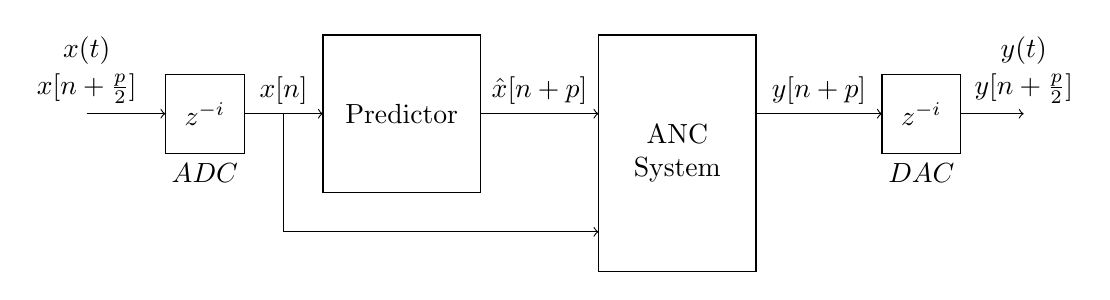
\begin{tikzpicture}
\draw  (-4,1.5) rectangle node {$z^{-i}$} (-5,0.5);
\draw (-4.5,0) node[above]{$ADC$} ;

\draw  (-3,2) rectangle  node[align=center] {Predictor} (-1,0) ;

\draw  (0.5,2) rectangle node[text width=1.5cm,align=center] {ANC System}(2.5,-1);
\draw  (4.1,1.5) rectangle node {$z^{-i}$}(5.1,0.5);
\draw (4.6,0) node[above]{$DAC$} ;

\draw [->](-4,1)  -- (-3,1);


\draw [->](-1,1)  -- node[above]{$\hat{x}[n+p]$}  (0.5,1);
\draw [->](2.5,1) -- node[above]{$y[n+p]$} (4.1,1);

\draw [->](-6,1) node[above]{$x[n+\frac{p}{2}]$} -- (-5,1);
\draw (-6,1.5) node[above]{$x(t)$} ;
\draw [->](5.1,1)-- (5.9,1) node[above]{$y[n+\frac{p}{2}]$} ;
\draw [->](-3.5,1) node[above]{$x[n]$} -- (-3.5,-0.5) -- (0.5,-0.5);
\draw (5.9,1.5) node[above]{$y(t)$} ;
\end{tikzpicture}}	
	\end{center}
\end{frame}

\section{Oliver}
\begin{frame}
	\frametitle{Oliver Job}
	\tableofcontents[currentsection]
\end{frame}
\subsection{herpa derp derp}
\begin{frame}{This is Ojo's part}{Me Ojo, you Jane}		
	\begin{columns}
		\begin{column}{0.5\textwidth}
		fish can be both blue and green	
		\end{column}
		\begin{column}{0.5\textwidth} 
		\begin{itemize}
			\item<1-> Blue fish
			\item<2-> Green fish
			\item<3-> But can we neglect the purple fish?
			\begin{itemize}
				\item<4-> Yes, because they are gay
			\end{itemize}			
		\end{itemize}		
		\end{column}
	\end{columns}
\end{frame}
%\section{Christian}
\begin{frame}
	\frametitle{Christian Job}
	\tableofcontents[currentsection]
\end{frame}
\subsection{What is Active Noise Control (ANC)}
\begin{frame}{This is christians part}{some fancy subtitle}		
	\begin{columns}
		\begin{column}{0.5\textwidth}
		fish can be both blue and green	
		\end{column}
		\begin{column}{0.5\textwidth} 
		\begin{itemize}
			\item<1-> Blue fish
			\item<2-> Green fish
			\item<3-> But can we neglect the purple fish?
			\begin{itemize}
				\item<4-> Yes, because they are gay
			\end{itemize}			
		\end{itemize}		
		\end{column}
	\end{columns}
\end{frame}
%\section{Filtered-x Least mean squares}

\begin{frame}{Filtered-x Least mean squares}{by Mikkel}
	\small
	\tableofcontents[currentsection, hideothersubsections]	
\end{frame}
\subsection{The general system}
\begin{frame}{Filtered-$x$ Least mean squares}{The General System}
	\begin{columns}
		\begin{column}{0.5\textwidth}		

		\begin{itemize}
		\item Feedforward
		\item Combined with an error microphone for feedback
		\begin{itemize}
		\item Adapt to changes in environment
		\item Using FIR filter		
		\end{itemize}
		\item Assumptions:
		\begin{itemize}
		\item Stationary Cancellation path
		\end{itemize}

		\begin{itemize}
			\setlength{\itemindent}{4em}
			\item[Input] $x[n]$
			\item[Output]$y[n]$
			\item[Error] $e[n]$	
			\item[Filtered x] $f[n]$
			\item[Filter coefficients] $b[n]$	
			\item[Cancellation Path] $H_{cp}[n]$		
		\end{itemize}

		\end{itemize}

		
		\end{column}
		\begin{column}{0.5\textwidth}
		\resizebox{1.1\columnwidth}{!}{	
		\begin{tikzpicture}
\draw [](-2.92,2.32) node (v1) {} .. controls (-3.26,2.06) and (-3.26,0.54) .. (-2.92,0.32) node (v2) {};

\draw [draw=black,fill=black!20](-0.68,2.32) node (v1) {} .. controls (-1.08,2.06) and (-1.08,0.54) .. (-0.68,0.32) node (v2) {};
\draw [white, fill=black!20](-0.68,2.32) -- (1.56,2.32) -- (1.56,0.32) -- (-0.68,0.32);


\draw [draw=black,fill=black!60](-0.93,1.78) node (v1) {} .. controls (-0.99,1.59) and (-0.99,1.14) .. (-0.95,0.94) node (v2) {};
\draw [draw=black,fill=black!60](-0.93,1.78) -- (0.72,1.78) -- (0.72,0.94) -- (-0.95,0.94);


\draw [draw=black,fill=white] (0.48,1.36) node (v3) {3} ellipse (0.2 and 0.3);
\draw [draw=black,fill=black](0.28,1.66) -- (0.28,1.06);

\draw [draw=black,fill=white] (-3.4,1.36) node (v3) {1} ellipse (0.2 and 0.3);
\draw [draw=black,fill=black](-3.6,1.7) -- (-3.6,1.06);


\draw [draw=black,fill=black] (-2.9,1.7) rectangle (-3,1);
\draw (-2.9,1.3) -- (-2.6,1.7) -- (-2.6,1) -- (-2.9,1.3);
\node at (-2.7,1.34) {\small{2}};
\node at (-1.7,1.54) {\small{c[n]}};

\draw[->,dashed] (-2.6,1.36) node[right=0.5,above]{\small{}}-- (0.28,1.36);



\draw [->](-1.14,-1.76) -- (-1.14,-0.2) -- (-2.94,-0.2) -- (-2.94,1);
\node at (0,2) {\small{Ear Canal}};
\node[anchor=south west,inner sep=0] at (1.9,0.3) {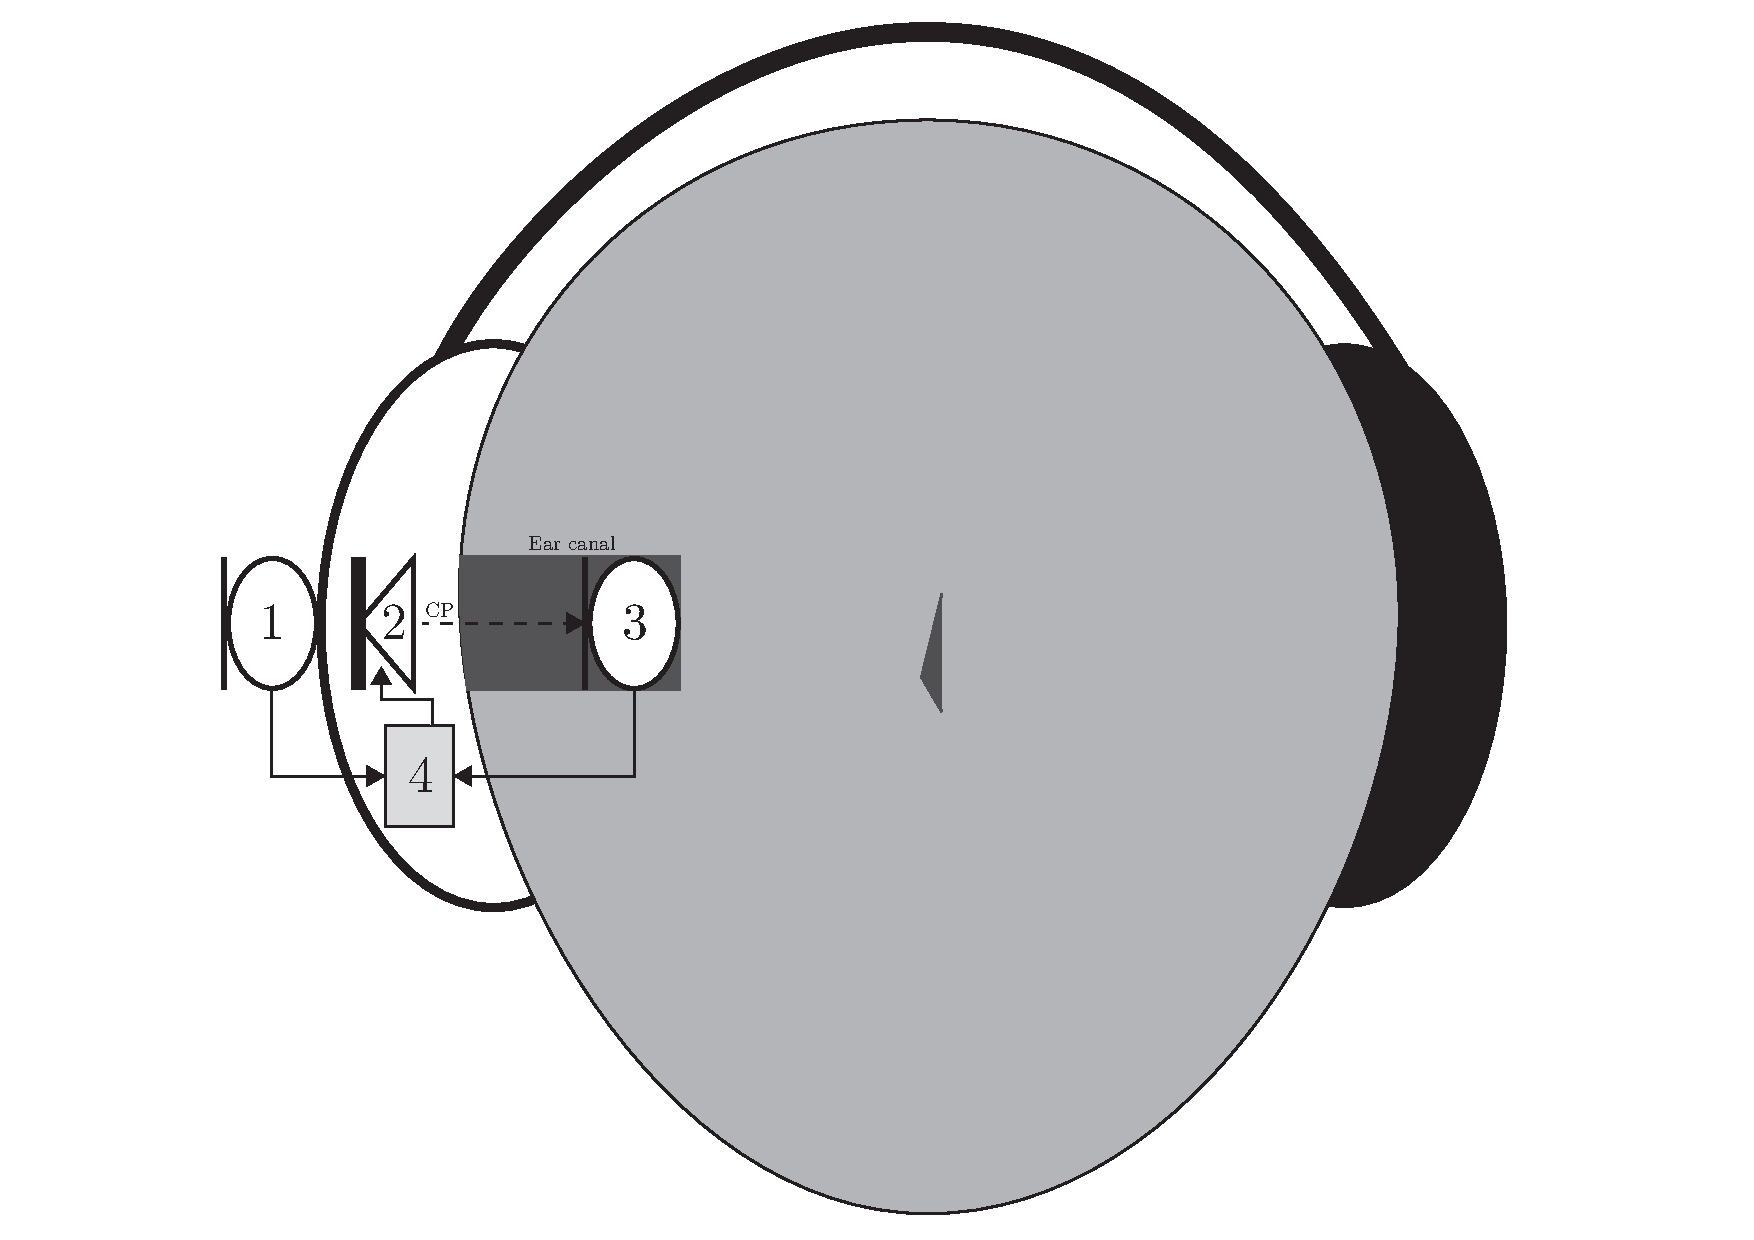
\includegraphics[width=3cm]{figures/BasicOverview}};

\draw  (3.14,1.65) rectangle (2.14,0.95);

\draw (1.56,1.31) -- (2.14,1.31);
\draw  (1.56,2.32) rectangle (-3.7,0.32);
\draw  (-5,-1.75) rectangle node[text width=2cm,align=center] {ADC \& Antialiasing filter} (-2.86,-3.25);
\draw  (-5,-6) rectangle node[text width=2.5cm,align=center] {Cancellation \\ path}(-2.75,-7.5);
\draw  (-1.23,-6) rectangle node[text width=2.5cm,align=center] {Adaptive FXLMS Algorithm} (1.27,-7.5);

\draw  (-3.45,-3.79) rectangle node[text width=1.5cm,align=center,fill=white] {Control filter} (-1.58,-5.29);
\draw  (-2.08,-1.75) rectangle node[text width=2.5cm,align=center] {DAC \& \\ Reconstruction filter}(0.37,-3.25);
\draw  (0.77,-1.75) rectangle node[text width=2cm,align=center] {ADC \& Antialiasing filter}(2.91,-3.25);

\draw  (-5.71,-0.69) rectangle (3.55,-7.76);
\node at (-5.06,-0.99) {DSP(4)};
\node [text width=2cm,align=center] at (-3.15,-1.2) {Reference Signal};

\draw[->] (-2.75,-7) -- node[above]{$f[n]$} (-1.23,-7);

\draw[->] (2.27,-3.25) -- node[right]{$e[n]$} (2.27,-7)  -- (1.27,-7);



\draw [->](-4,-3.25) -- (-4,-6);

\draw [->](-4,-4.79) node[left]{$x[n]$} -- (-3.45,-4.79);

\draw[->] (-1.58,-4.79) -- (-1.08,-4.79) --node[right]{$y[n]$} (-1.08,-3.25);

\node [text width=2cm,align=center] at (-0.38,-1.25) {Control Signal};
\node [text width=1.5cm,align=center] at (2.82,-1.25) {Error Signal};

\draw (-1.23,-6.4) -- (-1.83,-6.4) --node[above=3.25,right]{$\bar{b}[n+1]$} (-2.43,-5.29);
\draw [->](-3.1,-3.79) -- (-3.3,-3.43);


\draw[->] (0.48,1.06) -- (0.48,0) -- (2,0) -- (2,-1.76);
\draw[->] (-3.4,1.06) -- (-3.4,-0.16) -- (-4.2,-0.16) -- (-4.2,-1.76);
\end{tikzpicture}
		}
		\end{column}
	\end{columns}
\end{frame}


\subsection{Optimization}
\begin{frame}{Filtered-$x$ Least mean squares}{A minimization problem}
	\begin{columns}
		\begin{column}{0.5\textwidth}		
			
			\begin{itemize}
				\item[] Minimize $e^2[n]$
				\item[]
				\item[] Gradient descent method
				\begin{itemize}
					\item[] $\bar{b}[k+1]=\bar{b}[k]- \mu \nabla \bar{J}[n]$
				\end{itemize}
				 
			\end{itemize}
			
			
		\end{column}
		\begin{column}{0.5\textwidth}
			\resizebox{0.85\columnwidth}{!}{	
			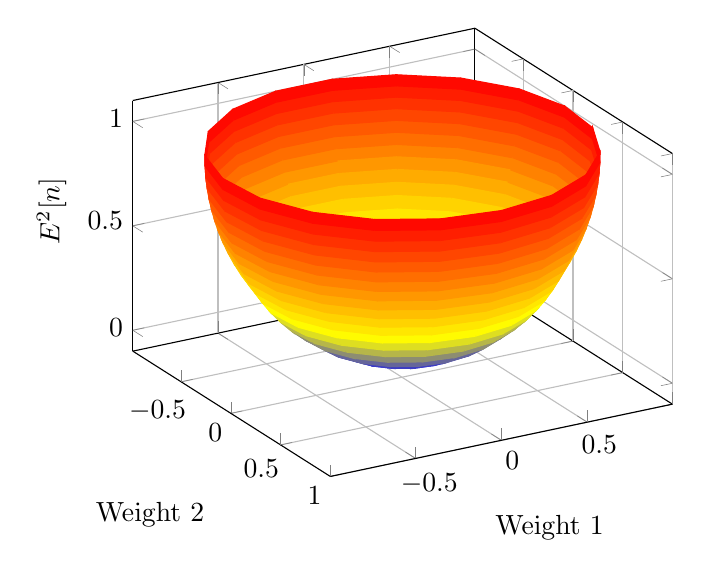
\begin{tikzpicture}
			\begin{axis}[
			view={60}{30},
			ylabel = {Weight 1},
			xlabel = {Weight 2},
			zlabel = {$E^2[n]$},
			zticklabels={1,0.5,0},ztick={0,-0.5,-1},
			grid=major,
			]
			\addplot3[surf,shader=flat,
			samples=20,
			domain=-1:0,y domain=0:2*pi,
			z buffer=sort]
			({sqrt(1-x^2) * cos(deg(y))},
			{sqrt( 1-x^2 ) * sin(deg(y))},
			x);	
			\end{axis}
			\end{tikzpicture}
			}
		\end{column}
	\end{columns}
\end{frame}


\begin{frame}{Filtered-$x$ Least mean squares}{Adaptive FXLMS Algorithm}

	\begin{columns}
		\begin{column}{0.5\textwidth}
		\begin{center}
		

		\begin{itemize}
		\item[] Error Source:
		\begin{itemize}
		\item Primary Noise $p[n]$
		\item Counterphase signal $s[n]$
		\item $e[n]=p[n]+s[n]$
		\end{itemize}
		\item[]
		\item[] Determining the gradient
		\begin{itemize}
		\item[] $\frac{\partial e^2[n]}{\partial b[n]}=2 \cdot e[n] \cdot \frac{\partial e[n]}{\partial b[n]} =2e[n] \cdot \frac{\partial s[n]}{\partial b[n]}$
		\end{itemize}
		\item[]
		\item[] Utilizing the Filtered-x
		\begin{itemize}
		\item[] $\frac{\partial s[n]}{\partial b[n]} = [b[n] * x[n]]* \hat{c}[n]$
		\end{itemize}			
		\end{itemize}
		\end{center}	
		
		
		
		
		\end{column}
		\begin{column}{0.5\textwidth}
		\resizebox{1\columnwidth}{!}{	
			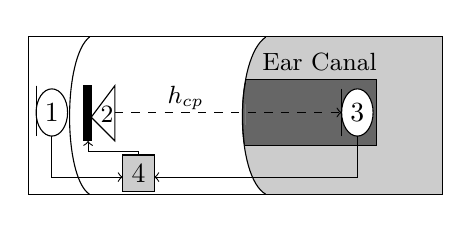
\begin{tikzpicture}
			\draw [](-2.92,2.32) node (v1) {} .. controls (-3.26,2.06) and (-3.26,0.54) .. (-2.92,0.32) node (v2) {};
			
			\draw [draw=black,fill=black!20](-0.68,2.32) node (v1) {} .. controls (-1.08,2.06) and (-1.08,0.54) .. (-0.68,0.32) node (v2) {};
			\draw [white, fill=black!20](-0.68,2.32) -- (1.56,2.32) -- (1.56,0.32) -- (-0.68,0.32);
			
			
			\draw [draw=black,fill=black!60](-0.93,1.78) node (v1) {} .. controls (-0.99,1.59) and (-0.99,1.14) .. (-0.95,0.94) node (v2) {};
			\draw [draw=black,fill=black!60](-0.93,1.78) -- (0.72,1.78) -- (0.72,0.94) -- (-0.95,0.94);
			
			
			\draw [draw=black,fill=white] (0.48,1.36) node (v3) {3} ellipse (0.2 and 0.3);
			\draw [draw=black,fill=black](0.28,1.66) -- (0.28,1.06);
			
			\draw [draw=black,fill=white] (-3.4,1.36) node (v3) {1} ellipse (0.2 and 0.3);
			\draw [draw=black,fill=black](-3.6,1.7) -- (-3.6,1.06);
			
			
			\draw [draw=black,fill=black] (-2.9,1.7) rectangle (-3,1);
			\draw (-2.9,1.3) -- (-2.6,1.7) -- (-2.6,1) -- (-2.9,1.3);
			\node at (-2.7,1.34) {\small{2}};
			
			
			\draw[->,dashed] (-2.6,1.36) node[right=0.5,above]{\small{}}-- (0.28,1.36);
			\draw[fill=black!20]  (-2.1,0.82) rectangle node{4}(-2.5,0.36);
			\draw [<-](-2.5,0.54) -- (-3.4,0.54) -- (-3.4,1.06);
			\draw [<-](-2.1,0.54) -- (0.48,0.54) -- (0.48,1.06);
			\draw [->](-2.3,0.82) -- (-2.3,0.86) -- (-2.94,0.86) -- (-2.94,1);
			\node at (0,2) {\small{Ear Canal}};
			\node at (-1.7,1.54) {\small{$h_{cp}$}};
			

			\draw  (1.56,2.32) rectangle (-3.7,0.32);
			\end{tikzpicture}
		}
		\end{column}
	\end{columns}


\end{frame}


\begin{frame}{Filtered-$x$ Least mean squares}{How did it perform}
	
	\begin{columns}
		\begin{column}{0.4\textwidth}			
				\begin{itemize}
					\item[] LMS expression:
							\begin{itemize}
								\item[] $b_j[n+1]=b_j[n]-2\mu e[n] f[n-j]$	
							\end{itemize}					
				\end{itemize}
	
			
			
			
			
		\end{column}
		\begin{column}{0.6\textwidth}
			\resizebox{1\columnwidth}{!}{	
		% This file was created by matlab2tikz.
%
%The latest updates can be retrieved from
%  http://www.mathworks.com/matlabcentral/fileexchange/22022-matlab2tikz-matlab2tikz
%where you can also make suggestions and rate matlab2tikz.
%
\definecolor{mycolor1}{rgb}{1.00000,1.00000,0.06667}%
\definecolor{mycolor2}{rgb}{0.68627,0.68627,0.68627}%
%
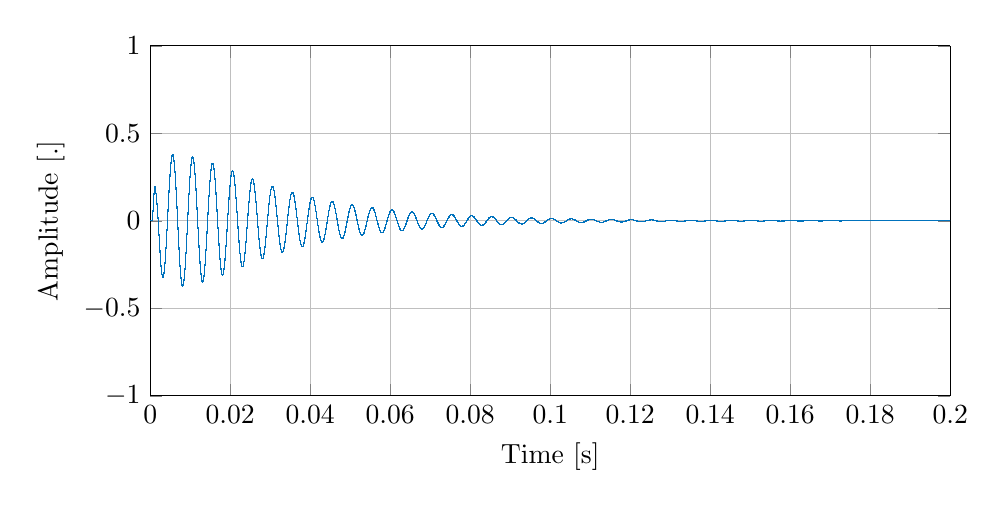
\begin{tikzpicture}

\begin{axis}[%
width=4in,
height=1.75in,
at={(0.27in,0.409in)},
scale only axis,
separate axis lines,
xmin=0,
xmax=0.20,
xlabel={Time [s]},
ylabel={{Amplitude [.]}},
xmajorgrids,
ymin=-1,
ymax=1,
ymajorgrids,
scaled y ticks = false,
y tick label style={/pgf/number format/fixed},
scaled x ticks = false,
x tick label style={/pgf/number format/fixed},
axis background/.style={fill=white}
]
\addplot[const plot,color=MATLABblue,solid,forget plot] plot table[row sep=crcr]{%
		0	0\\
		2.0833e-05	-4.8516e-07\\
		4.1667e-05	2.2008e-08\\
		6.25e-05	3.9358e-08\\
		8.3333e-05	7.1048e-07\\
		0.00010417	1.0655e-08\\
		0.000125	5.0776e-07\\
		0.00014583	-8.883e-08\\
		0.00016667	1.1933e-06\\
		0.0001875	-9.3284e-06\\
		0.00020833	-4.947e-05\\
		0.00022917	-8.7258e-05\\
		0.00025	-7.0082e-05\\
		0.00027083	1.906e-05\\
		0.00029167	0.00011492\\
		0.0003125	0.00015687\\
		0.00033333	0.00017446\\
		0.00035417	0.00023066\\
		0.000375	0.00035343\\
		0.00039583	0.00051387\\
		0.00041667	0.00066031\\
		0.0004375	0.00079\\
		0.00045833	0.000968\\
		0.00047917	0.0013845\\
		0.0005	0.0023623\\
		0.00052083	0.0042667\\
		0.00054167	0.0074175\\
		0.0005625	0.011996\\
		0.00058333	0.018042\\
		0.00060417	0.025409\\
		0.000625	0.033772\\
		0.00064583	0.042707\\
		0.00066667	0.051799\\
		0.0006875	0.060794\\
		0.00070833	0.069598\\
		0.00072917	0.078179\\
		0.00075	0.086603\\
		0.00077083	0.094951\\
		0.00079167	0.10324\\
		0.0008125	0.11146\\
		0.00083333	0.11963\\
		0.00085417	0.12771\\
		0.000875	0.13567\\
		0.00089583	0.14336\\
		0.00091667	0.1506\\
		0.0009375	0.15726\\
		0.00095833	0.16332\\
		0.00097917	0.16879\\
		0.001	0.1738\\
		0.0010208	0.17838\\
		0.0010417	0.18252\\
		0.0010625	0.18613\\
		0.0010833	0.18907\\
		0.0011042	0.1913\\
		0.001125	0.19281\\
		0.0011458	0.1936\\
		0.0011667	0.19367\\
		0.0011875	0.19303\\
		0.0012083	0.1917\\
		0.0012292	0.18978\\
		0.00125	0.18734\\
		0.0012708	0.18448\\
		0.0012917	0.1813\\
		0.0013125	0.17786\\
		0.0013333	0.1742\\
		0.0013542	0.17036\\
		0.001375	0.16638\\
		0.0013958	0.16231\\
		0.0014167	0.15814\\
		0.0014375	0.15386\\
		0.0014583	0.14945\\
		0.0014792	0.14489\\
		0.0015	0.14017\\
		0.0015208	0.1353\\
		0.0015417	0.13031\\
		0.0015625	0.1252\\
		0.0015833	0.11993\\
		0.0016042	0.1145\\
		0.001625	0.10891\\
		0.0016458	0.10319\\
		0.0016667	0.097352\\
		0.0016875	0.091391\\
		0.0017083	0.0853\\
		0.0017292	0.079088\\
		0.00175	0.072772\\
		0.0017708	0.066368\\
		0.0017917	0.059886\\
		0.0018125	0.053322\\
		0.0018333	0.046658\\
		0.0018542	0.039882\\
		0.001875	0.032971\\
		0.0018958	0.025914\\
		0.0019167	0.018706\\
		0.0019375	0.011353\\
		0.0019583	0.0038663\\
		0.0019792	-0.003751\\
		0.002	-0.011502\\
		0.0020208	-0.019375\\
		0.0020417	-0.027352\\
		0.0020625	-0.0354\\
		0.0020833	-0.0435\\
		0.0021042	-0.05166\\
		0.002125	-0.05988\\
		0.0021458	-0.068145\\
		0.0021667	-0.07643\\
		0.0021875	-0.08471\\
		0.0022083	-0.092972\\
		0.0022292	-0.10122\\
		0.00225	-0.10943\\
		0.0022708	-0.11759\\
		0.0022917	-0.12568\\
		0.0023125	-0.1337\\
		0.0023333	-0.14165\\
		0.0023542	-0.14953\\
		0.002375	-0.15731\\
		0.0023958	-0.16501\\
		0.0024167	-0.17262\\
		0.0024375	-0.18012\\
		0.0024583	-0.18753\\
		0.0024792	-0.19481\\
		0.0025	-0.20194\\
		0.0025208	-0.20894\\
		0.0025417	-0.21578\\
		0.0025625	-0.22246\\
		0.0025833	-0.22896\\
		0.0026042	-0.23526\\
		0.002625	-0.24137\\
		0.0026458	-0.24729\\
		0.0026667	-0.25301\\
		0.0026875	-0.25853\\
		0.0027083	-0.26382\\
		0.0027292	-0.26889\\
		0.00275	-0.27375\\
		0.0027708	-0.27839\\
		0.0027917	-0.28281\\
		0.0028125	-0.287\\
		0.0028333	-0.29095\\
		0.0028542	-0.29468\\
		0.002875	-0.29818\\
		0.0028958	-0.30145\\
		0.0029167	-0.30446\\
		0.0029375	-0.30723\\
		0.0029583	-0.30975\\
		0.0029792	-0.31203\\
		0.003	-0.31406\\
		0.0030208	-0.31584\\
		0.0030417	-0.31736\\
		0.0030625	-0.31864\\
		0.0030833	-0.31968\\
		0.0031042	-0.32047\\
		0.003125	-0.321\\
		0.0031458	-0.32126\\
		0.0031667	-0.32125\\
		0.0031875	-0.32097\\
		0.0032083	-0.32042\\
		0.0032292	-0.31959\\
		0.00325	-0.31849\\
		0.0032708	-0.31713\\
		0.0032917	-0.31552\\
		0.0033125	-0.31366\\
		0.0033333	-0.31155\\
		0.0033542	-0.30917\\
		0.003375	-0.30655\\
		0.0033958	-0.30368\\
		0.0034167	-0.30056\\
		0.0034375	-0.29718\\
		0.0034583	-0.29353\\
		0.0034792	-0.28962\\
		0.0035	-0.28548\\
		0.0035208	-0.28111\\
		0.0035417	-0.27651\\
		0.0035625	-0.27168\\
		0.0035833	-0.26663\\
		0.0036042	-0.26137\\
		0.003625	-0.25592\\
		0.0036458	-0.25025\\
		0.0036667	-0.24438\\
		0.0036875	-0.23831\\
		0.0037083	-0.23206\\
		0.0037292	-0.22563\\
		0.00375	-0.21902\\
		0.0037708	-0.21223\\
		0.0037917	-0.20526\\
		0.0038125	-0.19814\\
		0.0038333	-0.19087\\
		0.0038542	-0.18344\\
		0.003875	-0.17587\\
		0.0038958	-0.16815\\
		0.0039167	-0.1603\\
		0.0039375	-0.15233\\
		0.0039583	-0.14423\\
		0.0039792	-0.136\\
		0.004	-0.12765\\
		0.0040208	-0.1192\\
		0.0040417	-0.11064\\
		0.0040625	-0.102\\
		0.0040833	-0.093264\\
		0.0041042	-0.084454\\
		0.004125	-0.07558\\
		0.0041458	-0.066652\\
		0.0041667	-0.057667\\
		0.0041875	-0.048617\\
		0.0042083	-0.039502\\
		0.0042292	-0.030329\\
		0.00425	-0.021108\\
		0.0042708	-0.011848\\
		0.0042917	-0.002552\\
		0.0043125	0.0067658\\
		0.0043333	0.016088\\
		0.0043542	0.025402\\
		0.004375	0.034703\\
		0.0043958	0.043993\\
		0.0044167	0.053274\\
		0.0044375	0.062538\\
		0.0044583	0.071781\\
		0.0044792	0.080997\\
		0.0045	0.090186\\
		0.0045208	0.099339\\
		0.0045417	0.10845\\
		0.0045625	0.11749\\
		0.0045833	0.12645\\
		0.0046042	0.13534\\
		0.004625	0.14416\\
		0.0046458	0.15288\\
		0.0046667	0.16152\\
		0.0046875	0.17007\\
		0.0047083	0.17852\\
		0.0047292	0.18687\\
		0.00475	0.19512\\
		0.0047708	0.20325\\
		0.0047917	0.21126\\
		0.0048125	0.21913\\
		0.0048333	0.22686\\
		0.0048542	0.23446\\
		0.004875	0.2419\\
		0.0048958	0.24918\\
		0.0049167	0.25631\\
		0.0049375	0.26328\\
		0.0049583	0.27008\\
		0.0049792	0.27671\\
		0.005	0.28316\\
		0.0050208	0.28943\\
		0.0050417	0.29551\\
		0.0050625	0.30142\\
		0.0050833	0.30714\\
		0.0051042	0.31266\\
		0.005125	0.31798\\
		0.0051458	0.32311\\
		0.0051667	0.32804\\
		0.0051875	0.33277\\
		0.0052083	0.33728\\
		0.0052292	0.34159\\
		0.00525	0.34568\\
		0.0052708	0.34955\\
		0.0052917	0.35319\\
		0.0053125	0.3566\\
		0.0053333	0.35978\\
		0.0053542	0.36273\\
		0.005375	0.36545\\
		0.0053958	0.36794\\
		0.0054167	0.37019\\
		0.0054375	0.37219\\
		0.0054583	0.37395\\
		0.0054792	0.37546\\
		0.0055	0.37669\\
		0.0055208	0.37766\\
		0.0055417	0.37834\\
		0.0055625	0.37877\\
		0.0055833	0.37894\\
		0.0056042	0.37884\\
		0.005625	0.37848\\
		0.0056458	0.37786\\
		0.0056667	0.37698\\
		0.0056875	0.37585\\
		0.0057083	0.37446\\
		0.0057292	0.3728\\
		0.00575	0.37086\\
		0.0057708	0.36865\\
		0.0057917	0.36619\\
		0.0058125	0.36347\\
		0.0058333	0.3605\\
		0.0058542	0.35728\\
		0.005875	0.35382\\
		0.0058958	0.35012\\
		0.0059167	0.34619\\
		0.0059375	0.34203\\
		0.0059583	0.33763\\
		0.0059792	0.33301\\
		0.006	0.32817\\
		0.0060208	0.32311\\
		0.0060417	0.31783\\
		0.0060625	0.31234\\
		0.0060833	0.30664\\
		0.0061042	0.30075\\
		0.006125	0.29466\\
		0.0061458	0.28837\\
		0.0061667	0.28187\\
		0.0061875	0.27519\\
		0.0062083	0.26831\\
		0.0062292	0.26126\\
		0.00625	0.25402\\
		0.0062708	0.2466\\
		0.0062917	0.239\\
		0.0063125	0.23124\\
		0.0063333	0.22332\\
		0.0063542	0.21524\\
		0.006375	0.207\\
		0.0063958	0.19861\\
		0.0064167	0.19008\\
		0.0064375	0.18142\\
		0.0064583	0.17263\\
		0.0064792	0.16372\\
		0.0065	0.15469\\
		0.0065208	0.14555\\
		0.0065417	0.13632\\
		0.0065625	0.12699\\
		0.0065833	0.11757\\
		0.0066042	0.10806\\
		0.006625	0.098485\\
		0.0066458	0.088848\\
		0.0066667	0.079151\\
		0.0066875	0.069396\\
		0.0067083	0.059589\\
		0.0067292	0.04974\\
		0.00675	0.039859\\
		0.0067708	0.029947\\
		0.0067917	0.020006\\
		0.0068125	0.010047\\
		0.0068333	8.5286e-05\\
		0.0068542	-0.0098689\\
		0.006875	-0.019812\\
		0.0068958	-0.029744\\
		0.0069167	-0.039659\\
		0.0069375	-0.049544\\
		0.0069583	-0.059388\\
		0.0069792	-0.069189\\
		0.007	-0.078946\\
		0.0070208	-0.088654\\
		0.0070417	-0.098298\\
		0.0070625	-0.10787\\
		0.0070833	-0.11736\\
		0.0071042	-0.12676\\
		0.007125	-0.13607\\
		0.0071458	-0.14528\\
		0.0071667	-0.15438\\
		0.0071875	-0.16336\\
		0.0072083	-0.17223\\
		0.0072292	-0.18098\\
		0.00725	-0.1896\\
		0.0072708	-0.19807\\
		0.0072917	-0.2064\\
		0.0073125	-0.21458\\
		0.0073333	-0.22261\\
		0.0073542	-0.23048\\
		0.007375	-0.23817\\
		0.0073958	-0.24569\\
		0.0074167	-0.25303\\
		0.0074375	-0.26019\\
		0.0074583	-0.26717\\
		0.0074792	-0.27397\\
		0.0075	-0.28056\\
		0.0075208	-0.28697\\
		0.0075417	-0.29317\\
		0.0075625	-0.29918\\
		0.0075833	-0.30498\\
		0.0076042	-0.31056\\
		0.007625	-0.31592\\
		0.0076458	-0.32108\\
		0.0076667	-0.32601\\
		0.0076875	-0.33072\\
		0.0077083	-0.33519\\
		0.0077292	-0.33943\\
		0.00775	-0.34344\\
		0.0077708	-0.34722\\
		0.0077917	-0.35076\\
		0.0078125	-0.35405\\
		0.0078333	-0.3571\\
		0.0078542	-0.35991\\
		0.007875	-0.36248\\
		0.0078958	-0.3648\\
		0.0079167	-0.36686\\
		0.0079375	-0.36868\\
		0.0079583	-0.37025\\
		0.0079792	-0.37158\\
		0.008	-0.37266\\
		0.0080208	-0.37348\\
		0.0080417	-0.37405\\
		0.0080625	-0.37437\\
		0.0080833	-0.37444\\
		0.0081042	-0.37426\\
		0.008125	-0.37383\\
		0.0081458	-0.37313\\
		0.0081667	-0.37219\\
		0.0081875	-0.37101\\
		0.0082083	-0.36957\\
		0.0082292	-0.36787\\
		0.00825	-0.36592\\
		0.0082708	-0.36373\\
		0.0082917	-0.36129\\
		0.0083125	-0.35862\\
		0.0083333	-0.35569\\
		0.0083542	-0.35253\\
		0.008375	-0.34913\\
		0.0083958	-0.34551\\
		0.0084167	-0.34165\\
		0.0084375	-0.33756\\
		0.0084583	-0.33324\\
		0.0084792	-0.32869\\
		0.0085	-0.32392\\
		0.0085208	-0.31894\\
		0.0085417	-0.31373\\
		0.0085625	-0.30831\\
		0.0085833	-0.30268\\
		0.0086042	-0.29686\\
		0.008625	-0.29083\\
		0.0086458	-0.2846\\
		0.0086667	-0.27817\\
		0.0086875	-0.27156\\
		0.0087083	-0.26477\\
		0.0087292	-0.25779\\
		0.00875	-0.25065\\
		0.0087708	-0.24333\\
		0.0087917	-0.23585\\
		0.0088125	-0.22822\\
		0.0088333	-0.22044\\
		0.0088542	-0.21251\\
		0.008875	-0.20444\\
		0.0088958	-0.19623\\
		0.0089167	-0.18788\\
		0.0089375	-0.17942\\
		0.0089583	-0.17082\\
		0.0089792	-0.16211\\
		0.009	-0.15328\\
		0.0090208	-0.14436\\
		0.0090417	-0.13534\\
		0.0090625	-0.12623\\
		0.0090833	-0.11703\\
		0.0091042	-0.10775\\
		0.009125	-0.098395\\
		0.0091458	-0.088978\\
		0.0091667	-0.079504\\
		0.0091875	-0.069974\\
		0.0092083	-0.060398\\
		0.0092292	-0.050782\\
		0.00925	-0.041135\\
		0.0092708	-0.031461\\
		0.0092917	-0.021766\\
		0.0093125	-0.012055\\
		0.0093333	-0.0023365\\
		0.0093542	0.0073835\\
		0.009375	0.017101\\
		0.0093958	0.026812\\
		0.0094167	0.036507\\
		0.0094375	0.046175\\
		0.0094583	0.055805\\
		0.0094792	0.065393\\
		0.0095	0.074935\\
		0.0095208	0.084425\\
		0.0095417	0.093854\\
		0.0095625	0.10321\\
		0.0095833	0.11249\\
		0.0096042	0.12169\\
		0.009625	0.13081\\
		0.0096458	0.13983\\
		0.0096667	0.14875\\
		0.0096875	0.15756\\
		0.0097083	0.16626\\
		0.0097292	0.17483\\
		0.00975	0.18328\\
		0.0097708	0.19158\\
		0.0097917	0.19975\\
		0.0098125	0.20778\\
		0.0098333	0.21566\\
		0.0098542	0.22339\\
		0.009875	0.23095\\
		0.0098958	0.23836\\
		0.0099167	0.24559\\
		0.0099375	0.25266\\
		0.0099583	0.25956\\
		0.0099792	0.26627\\
		0.01	0.27279\\
		0.010021	0.27912\\
		0.010042	0.28526\\
		0.010063	0.2912\\
		0.010083	0.29693\\
		0.010104	0.30246\\
		0.010125	0.30777\\
		0.010146	0.31288\\
		0.010167	0.31777\\
		0.010188	0.32244\\
		0.010208	0.32688\\
		0.010229	0.33109\\
		0.01025	0.33508\\
		0.010271	0.33883\\
		0.010292	0.34235\\
		0.010313	0.34562\\
		0.010333	0.34866\\
		0.010354	0.35146\\
		0.010375	0.35401\\
		0.010396	0.35633\\
		0.010417	0.35839\\
		0.010437	0.36021\\
		0.010458	0.36178\\
		0.010479	0.36309\\
		0.0105	0.36415\\
		0.010521	0.36495\\
		0.010542	0.36549\\
		0.010562	0.36578\\
		0.010583	0.36581\\
		0.010604	0.36559\\
		0.010625	0.36511\\
		0.010646	0.36438\\
		0.010667	0.36339\\
		0.010687	0.36216\\
		0.010708	0.36067\\
		0.010729	0.35893\\
		0.01075	0.35693\\
		0.010771	0.3547\\
		0.010792	0.35222\\
		0.010812	0.34951\\
		0.010833	0.34656\\
		0.010854	0.34338\\
		0.010875	0.33997\\
		0.010896	0.33634\\
		0.010917	0.33249\\
		0.010937	0.32841\\
		0.010958	0.3241\\
		0.010979	0.31958\\
		0.011	0.31484\\
		0.011021	0.3099\\
		0.011042	0.30474\\
		0.011062	0.29938\\
		0.011083	0.29382\\
		0.011104	0.28807\\
		0.011125	0.28214\\
		0.011146	0.27602\\
		0.011167	0.26972\\
		0.011188	0.26324\\
		0.011208	0.2566\\
		0.011229	0.24978\\
		0.01125	0.2428\\
		0.011271	0.23566\\
		0.011292	0.22836\\
		0.011313	0.22091\\
		0.011333	0.21331\\
		0.011354	0.20557\\
		0.011375	0.19769\\
		0.011396	0.18968\\
		0.011417	0.18155\\
		0.011438	0.1733\\
		0.011458	0.16493\\
		0.011479	0.15645\\
		0.0115	0.14786\\
		0.011521	0.13917\\
		0.011542	0.1304\\
		0.011563	0.12153\\
		0.011583	0.11258\\
		0.011604	0.10356\\
		0.011625	0.094471\\
		0.011646	0.08533\\
		0.011667	0.076138\\
		0.011688	0.066899\\
		0.011708	0.057621\\
		0.011729	0.048312\\
		0.01175	0.038979\\
		0.011771	0.029624\\
		0.011792	0.020253\\
		0.011813	0.010872\\
		0.011833	0.0014917\\
		0.011854	-0.0078831\\
		0.011875	-0.017247\\
		0.011896	-0.026593\\
		0.011917	-0.035911\\
		0.011938	-0.045194\\
		0.011958	-0.054433\\
		0.011979	-0.063626\\
		0.012	-0.072768\\
		0.012021	-0.081855\\
		0.012042	-0.090875\\
		0.012063	-0.099821\\
		0.012083	-0.10869\\
		0.012104	-0.11747\\
		0.012125	-0.12616\\
		0.012146	-0.13476\\
		0.012167	-0.14325\\
		0.012188	-0.15164\\
		0.012208	-0.15992\\
		0.012229	-0.16808\\
		0.01225	-0.17612\\
		0.012271	-0.18404\\
		0.012292	-0.19182\\
		0.012312	-0.19947\\
		0.012333	-0.20698\\
		0.012354	-0.21434\\
		0.012375	-0.22155\\
		0.012396	-0.2286\\
		0.012417	-0.2355\\
		0.012437	-0.24223\\
		0.012458	-0.24879\\
		0.012479	-0.25517\\
		0.0125	-0.26138\\
		0.012521	-0.26741\\
		0.012542	-0.27325\\
		0.012562	-0.2789\\
		0.012583	-0.28436\\
		0.012604	-0.28963\\
		0.012625	-0.29469\\
		0.012646	-0.29956\\
		0.012667	-0.30422\\
		0.012687	-0.30866\\
		0.012708	-0.3129\\
		0.012729	-0.31691\\
		0.01275	-0.32071\\
		0.012771	-0.32429\\
		0.012792	-0.32763\\
		0.012812	-0.33075\\
		0.012833	-0.33364\\
		0.012854	-0.3363\\
		0.012875	-0.33872\\
		0.012896	-0.34091\\
		0.012917	-0.34285\\
		0.012937	-0.34456\\
		0.012958	-0.34602\\
		0.012979	-0.34724\\
		0.013	-0.34821\\
		0.013021	-0.34894\\
		0.013042	-0.34942\\
		0.013062	-0.34966\\
		0.013083	-0.34966\\
		0.013104	-0.34941\\
		0.013125	-0.34891\\
		0.013146	-0.34817\\
		0.013167	-0.34719\\
		0.013188	-0.34596\\
		0.013208	-0.34449\\
		0.013229	-0.34279\\
		0.01325	-0.34085\\
		0.013271	-0.33867\\
		0.013292	-0.33627\\
		0.013313	-0.33363\\
		0.013333	-0.33076\\
		0.013354	-0.32767\\
		0.013375	-0.32435\\
		0.013396	-0.32082\\
		0.013417	-0.31707\\
		0.013438	-0.31311\\
		0.013458	-0.30893\\
		0.013479	-0.30454\\
		0.0135	-0.29996\\
		0.013521	-0.29516\\
		0.013542	-0.29017\\
		0.013563	-0.28498\\
		0.013583	-0.2796\\
		0.013604	-0.27403\\
		0.013625	-0.26829\\
		0.013646	-0.26237\\
		0.013667	-0.25628\\
		0.013688	-0.25002\\
		0.013708	-0.24361\\
		0.013729	-0.23703\\
		0.01375	-0.2303\\
		0.013771	-0.22342\\
		0.013792	-0.21638\\
		0.013813	-0.20921\\
		0.013833	-0.20189\\
		0.013854	-0.19444\\
		0.013875	-0.18686\\
		0.013896	-0.17916\\
		0.013917	-0.17135\\
		0.013938	-0.16343\\
		0.013958	-0.1554\\
		0.013979	-0.14727\\
		0.014	-0.13905\\
		0.014021	-0.13073\\
		0.014042	-0.12233\\
		0.014063	-0.11385\\
		0.014083	-0.10529\\
		0.014104	-0.096671\\
		0.014125	-0.087988\\
		0.014146	-0.079252\\
		0.014167	-0.070467\\
		0.014187	-0.061639\\
		0.014208	-0.052775\\
		0.014229	-0.043885\\
		0.01425	-0.034971\\
		0.014271	-0.026038\\
		0.014292	-0.017091\\
		0.014312	-0.00814\\
		0.014333	0.0008065\\
		0.014354	0.0097418\\
		0.014375	0.01866\\
		0.014396	0.027556\\
		0.014417	0.036421\\
		0.014437	0.045246\\
		0.014458	0.054025\\
		0.014479	0.062755\\
		0.0145	0.071431\\
		0.014521	0.080046\\
		0.014542	0.088593\\
		0.014562	0.097067\\
		0.014583	0.10547\\
		0.014604	0.11378\\
		0.014625	0.12202\\
		0.014646	0.13016\\
		0.014667	0.13819\\
		0.014687	0.14613\\
		0.014708	0.15396\\
		0.014729	0.16168\\
		0.01475	0.16928\\
		0.014771	0.17675\\
		0.014792	0.1841\\
		0.014812	0.19132\\
		0.014833	0.1984\\
		0.014854	0.20533\\
		0.014875	0.21212\\
		0.014896	0.21876\\
		0.014917	0.22524\\
		0.014937	0.23157\\
		0.014958	0.23773\\
		0.014979	0.24372\\
		0.015	0.24954\\
		0.015021	0.25518\\
		0.015042	0.26065\\
		0.015063	0.26594\\
		0.015083	0.27103\\
		0.015104	0.27594\\
		0.015125	0.28065\\
		0.015146	0.28516\\
		0.015167	0.28946\\
		0.015188	0.29356\\
		0.015208	0.29745\\
		0.015229	0.30113\\
		0.01525	0.30459\\
		0.015271	0.30783\\
		0.015292	0.31086\\
		0.015313	0.31366\\
		0.015333	0.31624\\
		0.015354	0.31861\\
		0.015375	0.32075\\
		0.015396	0.32267\\
		0.015417	0.32435\\
		0.015438	0.32582\\
		0.015458	0.32705\\
		0.015479	0.32806\\
		0.0155	0.32884\\
		0.015521	0.32939\\
		0.015542	0.32972\\
		0.015563	0.32982\\
		0.015583	0.32969\\
		0.015604	0.32933\\
		0.015625	0.32875\\
		0.015646	0.32795\\
		0.015667	0.32693\\
		0.015688	0.32569\\
		0.015708	0.32423\\
		0.015729	0.32255\\
		0.01575	0.32066\\
		0.015771	0.31855\\
		0.015792	0.31623\\
		0.015813	0.31369\\
		0.015833	0.31094\\
		0.015854	0.30798\\
		0.015875	0.30481\\
		0.015896	0.30144\\
		0.015917	0.29787\\
		0.015938	0.29409\\
		0.015958	0.29012\\
		0.015979	0.28596\\
		0.016	0.2816\\
		0.016021	0.27705\\
		0.016042	0.27231\\
		0.016063	0.26738\\
		0.016083	0.26228\\
		0.016104	0.257\\
		0.016125	0.25154\\
		0.016146	0.24591\\
		0.016167	0.24011\\
		0.016188	0.23416\\
		0.016208	0.22805\\
		0.016229	0.22179\\
		0.01625	0.21537\\
		0.016271	0.20882\\
		0.016292	0.20212\\
		0.016313	0.1953\\
		0.016333	0.18835\\
		0.016354	0.18128\\
		0.016375	0.17408\\
		0.016396	0.16678\\
		0.016417	0.15937\\
		0.016438	0.15185\\
		0.016458	0.14424\\
		0.016479	0.13654\\
		0.0165	0.12875\\
		0.016521	0.12089\\
		0.016542	0.11295\\
		0.016563	0.10495\\
		0.016583	0.09688\\
		0.016604	0.088759\\
		0.016625	0.08059\\
		0.016646	0.072375\\
		0.016667	0.064116\\
		0.016688	0.05582\\
		0.016708	0.047494\\
		0.016729	0.039146\\
		0.01675	0.030779\\
		0.016771	0.022397\\
		0.016792	0.014006\\
		0.016813	0.0056142\\
		0.016833	-0.0027705\\
		0.016854	-0.011144\\
		0.016875	-0.019503\\
		0.016896	-0.027843\\
		0.016917	-0.036154\\
		0.016938	-0.044431\\
		0.016958	-0.052668\\
		0.016979	-0.060864\\
		0.017	-0.069013\\
		0.017021	-0.077106\\
		0.017042	-0.085136\\
		0.017062	-0.093097\\
		0.017083	-0.10099\\
		0.017104	-0.1088\\
		0.017125	-0.11652\\
		0.017146	-0.12416\\
		0.017167	-0.13169\\
		0.017187	-0.13913\\
		0.017208	-0.14646\\
		0.017229	-0.15369\\
		0.01725	-0.1608\\
		0.017271	-0.16779\\
		0.017292	-0.17466\\
		0.017312	-0.1814\\
		0.017333	-0.18801\\
		0.017354	-0.19449\\
		0.017375	-0.20082\\
		0.017396	-0.20701\\
		0.017417	-0.21305\\
		0.017437	-0.21894\\
		0.017458	-0.22466\\
		0.017479	-0.23023\\
		0.0175	-0.23562\\
		0.017521	-0.24085\\
		0.017542	-0.24592\\
		0.017562	-0.2508\\
		0.017583	-0.25551\\
		0.017604	-0.26004\\
		0.017625	-0.26439\\
		0.017646	-0.26856\\
		0.017667	-0.27254\\
		0.017687	-0.27633\\
		0.017708	-0.27992\\
		0.017729	-0.28332\\
		0.01775	-0.28652\\
		0.017771	-0.28952\\
		0.017792	-0.29232\\
		0.017812	-0.29492\\
		0.017833	-0.29731\\
		0.017854	-0.2995\\
		0.017875	-0.30148\\
		0.017896	-0.30325\\
		0.017917	-0.3048\\
		0.017937	-0.30615\\
		0.017958	-0.30728\\
		0.017979	-0.3082\\
		0.018	-0.30891\\
		0.018021	-0.3094\\
		0.018042	-0.30968\\
		0.018062	-0.30975\\
		0.018083	-0.3096\\
		0.018104	-0.30924\\
		0.018125	-0.30866\\
		0.018146	-0.30787\\
		0.018167	-0.30687\\
		0.018187	-0.30566\\
		0.018208	-0.30424\\
		0.018229	-0.30261\\
		0.01825	-0.30077\\
		0.018271	-0.29872\\
		0.018292	-0.29647\\
		0.018312	-0.29401\\
		0.018333	-0.29136\\
		0.018354	-0.2885\\
		0.018375	-0.28545\\
		0.018396	-0.2822\\
		0.018417	-0.27877\\
		0.018437	-0.27514\\
		0.018458	-0.27133\\
		0.018479	-0.26734\\
		0.0185	-0.26316\\
		0.018521	-0.25882\\
		0.018542	-0.25429\\
		0.018562	-0.2496\\
		0.018583	-0.24474\\
		0.018604	-0.23973\\
		0.018625	-0.23455\\
		0.018646	-0.22922\\
		0.018667	-0.22374\\
		0.018687	-0.21812\\
		0.018708	-0.21236\\
		0.018729	-0.20646\\
		0.01875	-0.20043\\
		0.018771	-0.19427\\
		0.018792	-0.18798\\
		0.018812	-0.18158\\
		0.018833	-0.17506\\
		0.018854	-0.16843\\
		0.018875	-0.16169\\
		0.018896	-0.15485\\
		0.018917	-0.14791\\
		0.018937	-0.14088\\
		0.018958	-0.13376\\
		0.018979	-0.12655\\
		0.019	-0.11927\\
		0.019021	-0.11191\\
		0.019042	-0.10449\\
		0.019063	-0.096993\\
		0.019083	-0.089439\\
		0.019104	-0.08183\\
		0.019125	-0.074173\\
		0.019146	-0.06647\\
		0.019167	-0.058727\\
		0.019188	-0.05095\\
		0.019208	-0.043148\\
		0.019229	-0.035327\\
		0.01925	-0.027492\\
		0.019271	-0.019645\\
		0.019292	-0.011795\\
		0.019313	-0.0039474\\
		0.019333	0.0038896\\
		0.019354	0.011712\\
		0.019375	0.019517\\
		0.019396	0.027296\\
		0.019417	0.035045\\
		0.019438	0.042755\\
		0.019458	0.050423\\
		0.019479	0.058045\\
		0.0195	0.065616\\
		0.019521	0.073129\\
		0.019542	0.080576\\
		0.019563	0.087954\\
		0.019583	0.09526\\
		0.019604	0.10249\\
		0.019625	0.10963\\
		0.019646	0.11668\\
		0.019667	0.12364\\
		0.019688	0.13051\\
		0.019708	0.13727\\
		0.019729	0.14393\\
		0.01975	0.15049\\
		0.019771	0.15693\\
		0.019792	0.16325\\
		0.019813	0.16946\\
		0.019833	0.17554\\
		0.019854	0.18149\\
		0.019875	0.18731\\
		0.019896	0.19299\\
		0.019917	0.19854\\
		0.019938	0.20394\\
		0.019958	0.2092\\
		0.019979	0.2143\\
		0.02	0.21925\\
		0.020021	0.22405\\
		0.020042	0.22869\\
		0.020063	0.23316\\
		0.020083	0.23746\\
		0.020104	0.2416\\
		0.020125	0.24557\\
		0.020146	0.24936\\
		0.020167	0.25299\\
		0.020188	0.25642\\
		0.020208	0.25968\\
		0.020229	0.26275\\
		0.02025	0.26564\\
		0.020271	0.26834\\
		0.020292	0.27086\\
		0.020313	0.27319\\
		0.020333	0.27533\\
		0.020354	0.27728\\
		0.020375	0.27904\\
		0.020396	0.28061\\
		0.020417	0.28199\\
		0.020438	0.28317\\
		0.020458	0.28415\\
		0.020479	0.28494\\
		0.0205	0.28553\\
		0.020521	0.28592\\
		0.020542	0.28612\\
		0.020563	0.28612\\
		0.020583	0.28592\\
		0.020604	0.28552\\
		0.020625	0.28493\\
		0.020646	0.28415\\
		0.020667	0.28316\\
		0.020688	0.28199\\
		0.020708	0.28062\\
		0.020729	0.27905\\
		0.02075	0.2773\\
		0.020771	0.27536\\
		0.020792	0.27323\\
		0.020812	0.27091\\
		0.020833	0.26841\\
		0.020854	0.26573\\
		0.020875	0.26286\\
		0.020896	0.25982\\
		0.020917	0.2566\\
		0.020937	0.25321\\
		0.020958	0.24965\\
		0.020979	0.24592\\
		0.021	0.24202\\
		0.021021	0.23796\\
		0.021042	0.23375\\
		0.021062	0.22937\\
		0.021083	0.22485\\
		0.021104	0.22017\\
		0.021125	0.21535\\
		0.021146	0.21039\\
		0.021167	0.20529\\
		0.021187	0.20005\\
		0.021208	0.19469\\
		0.021229	0.1892\\
		0.02125	0.18358\\
		0.021271	0.17785\\
		0.021292	0.172\\
		0.021312	0.16604\\
		0.021333	0.15997\\
		0.021354	0.15381\\
		0.021375	0.14754\\
		0.021396	0.14118\\
		0.021417	0.13474\\
		0.021437	0.1282\\
		0.021458	0.12159\\
		0.021479	0.11491\\
		0.0215	0.10816\\
		0.021521	0.10134\\
		0.021542	0.094456\\
		0.021562	0.087521\\
		0.021583	0.080535\\
		0.021604	0.073503\\
		0.021625	0.066431\\
		0.021646	0.059322\\
		0.021667	0.052183\\
		0.021687	0.045018\\
		0.021708	0.037831\\
		0.021729	0.030629\\
		0.02175	0.023416\\
		0.021771	0.016196\\
		0.021792	0.0089762\\
		0.021812	0.0017598\\
		0.021833	-0.0054475\\
		0.021854	-0.012641\\
		0.021875	-0.019815\\
		0.021896	-0.026965\\
		0.021917	-0.034087\\
		0.021937	-0.041175\\
		0.021958	-0.048225\\
		0.021979	-0.055231\\
		0.022	-0.062189\\
		0.022021	-0.069094\\
		0.022042	-0.075942\\
		0.022062	-0.082727\\
		0.022083	-0.089446\\
		0.022104	-0.096093\\
		0.022125	-0.10266\\
		0.022146	-0.10916\\
		0.022167	-0.11556\\
		0.022187	-0.12188\\
		0.022208	-0.12811\\
		0.022229	-0.13423\\
		0.02225	-0.14026\\
		0.022271	-0.14618\\
		0.022292	-0.15199\\
		0.022312	-0.15769\\
		0.022333	-0.16327\\
		0.022354	-0.16873\\
		0.022375	-0.17407\\
		0.022396	-0.17928\\
		0.022417	-0.18436\\
		0.022437	-0.1893\\
		0.022458	-0.19411\\
		0.022479	-0.19878\\
		0.0225	-0.2033\\
		0.022521	-0.20767\\
		0.022542	-0.2119\\
		0.022562	-0.21597\\
		0.022583	-0.21989\\
		0.022604	-0.22366\\
		0.022625	-0.22726\\
		0.022646	-0.2307\\
		0.022667	-0.23398\\
		0.022687	-0.23709\\
		0.022708	-0.24003\\
		0.022729	-0.2428\\
		0.02275	-0.24541\\
		0.022771	-0.24783\\
		0.022792	-0.25009\\
		0.022812	-0.25217\\
		0.022833	-0.25407\\
		0.022854	-0.2558\\
		0.022875	-0.25734\\
		0.022896	-0.25871\\
		0.022917	-0.2599\\
		0.022938	-0.2609\\
		0.022958	-0.26172\\
		0.022979	-0.26237\\
		0.023	-0.26283\\
		0.023021	-0.26311\\
		0.023042	-0.26321\\
		0.023063	-0.26312\\
		0.023083	-0.26286\\
		0.023104	-0.26241\\
		0.023125	-0.26179\\
		0.023146	-0.26098\\
		0.023167	-0.26\\
		0.023188	-0.25883\\
		0.023208	-0.2575\\
		0.023229	-0.25598\\
		0.02325	-0.2543\\
		0.023271	-0.25244\\
		0.023292	-0.2504\\
		0.023313	-0.2482\\
		0.023333	-0.24584\\
		0.023354	-0.2433\\
		0.023375	-0.2406\\
		0.023396	-0.23774\\
		0.023417	-0.23472\\
		0.023438	-0.23155\\
		0.023458	-0.22822\\
		0.023479	-0.22473\\
		0.0235	-0.2211\\
		0.023521	-0.21732\\
		0.023542	-0.2134\\
		0.023563	-0.20933\\
		0.023583	-0.20513\\
		0.023604	-0.2008\\
		0.023625	-0.19633\\
		0.023646	-0.19173\\
		0.023667	-0.18701\\
		0.023688	-0.18216\\
		0.023708	-0.1772\\
		0.023729	-0.17213\\
		0.02375	-0.16694\\
		0.023771	-0.16164\\
		0.023792	-0.15625\\
		0.023813	-0.15075\\
		0.023833	-0.14516\\
		0.023854	-0.13948\\
		0.023875	-0.1337\\
		0.023896	-0.12785\\
		0.023917	-0.12192\\
		0.023938	-0.11591\\
		0.023958	-0.10983\\
		0.023979	-0.10369\\
		0.024	-0.097483\\
		0.024021	-0.091219\\
		0.024042	-0.084902\\
		0.024063	-0.078537\\
		0.024083	-0.072128\\
		0.024104	-0.065679\\
		0.024125	-0.059194\\
		0.024146	-0.05268\\
		0.024167	-0.046139\\
		0.024188	-0.039576\\
		0.024208	-0.032997\\
		0.024229	-0.026405\\
		0.02425	-0.019806\\
		0.024271	-0.013203\\
		0.024292	-0.0066012\\
		0.024313	-5.5109e-06\\
		0.024333	0.0065797\\
		0.024354	0.01315\\
		0.024375	0.019701\\
		0.024396	0.026228\\
		0.024417	0.032726\\
		0.024438	0.039192\\
		0.024458	0.04562\\
		0.024479	0.052006\\
		0.0245	0.058347\\
		0.024521	0.064638\\
		0.024542	0.070874\\
		0.024562	0.077051\\
		0.024583	0.083165\\
		0.024604	0.089212\\
		0.024625	0.095188\\
		0.024646	0.10109\\
		0.024667	0.10691\\
		0.024687	0.11265\\
		0.024708	0.1183\\
		0.024729	0.12386\\
		0.02475	0.12933\\
		0.024771	0.1347\\
		0.024792	0.13997\\
		0.024812	0.14513\\
		0.024833	0.15018\\
		0.024854	0.15513\\
		0.024875	0.15996\\
		0.024896	0.16467\\
		0.024917	0.16925\\
		0.024937	0.17372\\
		0.024958	0.17806\\
		0.024979	0.18227\\
		0.025	0.18634\\
		0.025021	0.19028\\
		0.025042	0.19409\\
		0.025062	0.19775\\
		0.025083	0.20127\\
		0.025104	0.20465\\
		0.025125	0.20788\\
		0.025146	0.21096\\
		0.025167	0.2139\\
		0.025187	0.21668\\
		0.025208	0.2193\\
		0.025229	0.22177\\
		0.02525	0.22409\\
		0.025271	0.22624\\
		0.025292	0.22824\\
		0.025312	0.23007\\
		0.025333	0.23174\\
		0.025354	0.23326\\
		0.025375	0.2346\\
		0.025396	0.23579\\
		0.025417	0.23681\\
		0.025437	0.23766\\
		0.025458	0.23835\\
		0.025479	0.23887\\
		0.0255	0.23923\\
		0.025521	0.23942\\
		0.025542	0.23945\\
		0.025562	0.23931\\
		0.025583	0.23901\\
		0.025604	0.23854\\
		0.025625	0.23791\\
		0.025646	0.23712\\
		0.025667	0.23616\\
		0.025687	0.23504\\
		0.025708	0.23376\\
		0.025729	0.23233\\
		0.02575	0.23073\\
		0.025771	0.22898\\
		0.025792	0.22707\\
		0.025812	0.22501\\
		0.025833	0.2228\\
		0.025854	0.22044\\
		0.025875	0.21792\\
		0.025896	0.21527\\
		0.025917	0.21247\\
		0.025937	0.20952\\
		0.025958	0.20644\\
		0.025979	0.20322\\
		0.026	0.19986\\
		0.026021	0.19637\\
		0.026042	0.19275\\
		0.026062	0.18901\\
		0.026083	0.18514\\
		0.026104	0.18115\\
		0.026125	0.17704\\
		0.026146	0.17281\\
		0.026167	0.16847\\
		0.026187	0.16402\\
		0.026208	0.15947\\
		0.026229	0.15481\\
		0.02625	0.15006\\
		0.026271	0.14521\\
		0.026292	0.14026\\
		0.026312	0.13523\\
		0.026333	0.13011\\
		0.026354	0.12491\\
		0.026375	0.11963\\
		0.026396	0.11428\\
		0.026417	0.10886\\
		0.026437	0.10337\\
		0.026458	0.097817\\
		0.026479	0.092206\\
		0.0265	0.086541\\
		0.026521	0.080826\\
		0.026542	0.075063\\
		0.026562	0.069258\\
		0.026583	0.063415\\
		0.026604	0.057537\\
		0.026625	0.051628\\
		0.026646	0.045694\\
		0.026667	0.039737\\
		0.026687	0.033762\\
		0.026708	0.027774\\
		0.026729	0.021776\\
		0.02675	0.015772\\
		0.026771	0.0097671\\
		0.026792	0.0037649\\
		0.026813	-0.0022305\\
		0.026833	-0.0082147\\
		0.026854	-0.014184\\
		0.026875	-0.020134\\
		0.026896	-0.02606\\
		0.026917	-0.031959\\
		0.026938	-0.037827\\
		0.026958	-0.043659\\
		0.026979	-0.049452\\
		0.027	-0.055201\\
		0.027021	-0.060904\\
		0.027042	-0.066555\\
		0.027063	-0.072151\\
		0.027083	-0.077689\\
		0.027104	-0.083164\\
		0.027125	-0.088574\\
		0.027146	-0.093913\\
		0.027167	-0.099179\\
		0.027188	-0.10437\\
		0.027208	-0.10948\\
		0.027229	-0.1145\\
		0.02725	-0.11944\\
		0.027271	-0.12429\\
		0.027292	-0.12905\\
		0.027313	-0.1337\\
		0.027333	-0.13826\\
		0.027354	-0.14272\\
		0.027375	-0.14707\\
		0.027396	-0.15131\\
		0.027417	-0.15544\\
		0.027438	-0.15946\\
		0.027458	-0.16336\\
		0.027479	-0.16714\\
		0.0275	-0.1708\\
		0.027521	-0.17434\\
		0.027542	-0.17775\\
		0.027563	-0.18104\\
		0.027583	-0.18419\\
		0.027604	-0.18721\\
		0.027625	-0.1901\\
		0.027646	-0.19285\\
		0.027667	-0.19547\\
		0.027688	-0.19794\\
		0.027708	-0.20028\\
		0.027729	-0.20247\\
		0.02775	-0.20452\\
		0.027771	-0.20642\\
		0.027792	-0.20818\\
		0.027813	-0.2098\\
		0.027833	-0.21127\\
		0.027854	-0.21258\\
		0.027875	-0.21375\\
		0.027896	-0.21477\\
		0.027917	-0.21565\\
		0.027938	-0.21637\\
		0.027958	-0.21694\\
		0.027979	-0.21736\\
		0.028	-0.21763\\
		0.028021	-0.21775\\
		0.028042	-0.21771\\
		0.028063	-0.21753\\
		0.028083	-0.2172\\
		0.028104	-0.21672\\
		0.028125	-0.21609\\
		0.028146	-0.21532\\
		0.028167	-0.21439\\
		0.028188	-0.21332\\
		0.028208	-0.21211\\
		0.028229	-0.21075\\
		0.02825	-0.20924\\
		0.028271	-0.2076\\
		0.028292	-0.20581\\
		0.028312	-0.20389\\
		0.028333	-0.20182\\
		0.028354	-0.19963\\
		0.028375	-0.19729\\
		0.028396	-0.19483\\
		0.028417	-0.19223\\
		0.028437	-0.18951\\
		0.028458	-0.18666\\
		0.028479	-0.18369\\
		0.0285	-0.18059\\
		0.028521	-0.17737\\
		0.028542	-0.17404\\
		0.028562	-0.17059\\
		0.028583	-0.16703\\
		0.028604	-0.16336\\
		0.028625	-0.15959\\
		0.028646	-0.15571\\
		0.028667	-0.15173\\
		0.028687	-0.14765\\
		0.028708	-0.14347\\
		0.028729	-0.13921\\
		0.02875	-0.13485\\
		0.028771	-0.13041\\
		0.028792	-0.12588\\
		0.028812	-0.12128\\
		0.028833	-0.1166\\
		0.028854	-0.11184\\
		0.028875	-0.10702\\
		0.028896	-0.10213\\
		0.028917	-0.097177\\
		0.028937	-0.092165\\
		0.028958	-0.087098\\
		0.028979	-0.081979\\
		0.029	-0.076812\\
		0.029021	-0.071599\\
		0.029042	-0.066346\\
		0.029062	-0.061055\\
		0.029083	-0.055731\\
		0.029104	-0.050377\\
		0.029125	-0.044996\\
		0.029146	-0.039593\\
		0.029167	-0.034171\\
		0.029187	-0.028735\\
		0.029208	-0.023287\\
		0.029229	-0.017832\\
		0.02925	-0.012373\\
		0.029271	-0.0069144\\
		0.029292	-0.0014596\\
		0.029312	0.0039874\\
		0.029333	0.009423\\
		0.029354	0.014843\\
		0.029375	0.020245\\
		0.029396	0.025624\\
		0.029417	0.030977\\
		0.029437	0.0363\\
		0.029458	0.041589\\
		0.029479	0.046841\\
		0.0295	0.052053\\
		0.029521	0.05722\\
		0.029542	0.062339\\
		0.029562	0.067408\\
		0.029583	0.072422\\
		0.029604	0.077378\\
		0.029625	0.082272\\
		0.029646	0.087102\\
		0.029667	0.091864\\
		0.029687	0.096556\\
		0.029708	0.10117\\
		0.029729	0.10571\\
		0.02975	0.11017\\
		0.029771	0.11455\\
		0.029792	0.11884\\
		0.029812	0.12304\\
		0.029833	0.12715\\
		0.029854	0.13117\\
		0.029875	0.13509\\
		0.029896	0.13891\\
		0.029917	0.14263\\
		0.029937	0.14624\\
		0.029958	0.14975\\
		0.029979	0.15315\\
		0.03	0.15643\\
		0.030021	0.15961\\
		0.030042	0.16267\\
		0.030062	0.16561\\
		0.030083	0.16843\\
		0.030104	0.17113\\
		0.030125	0.17371\\
		0.030146	0.17617\\
		0.030167	0.1785\\
		0.030187	0.1807\\
		0.030208	0.18278\\
		0.030229	0.18472\\
		0.03025	0.18654\\
		0.030271	0.18822\\
		0.030292	0.18977\\
		0.030312	0.19119\\
		0.030333	0.19248\\
		0.030354	0.19363\\
		0.030375	0.19464\\
		0.030396	0.19552\\
		0.030417	0.19626\\
		0.030437	0.19686\\
		0.030458	0.19733\\
		0.030479	0.19766\\
		0.0305	0.19786\\
		0.030521	0.19792\\
		0.030542	0.19784\\
		0.030562	0.19762\\
		0.030583	0.19727\\
		0.030604	0.19679\\
		0.030625	0.19616\\
		0.030646	0.19541\\
		0.030667	0.19452\\
		0.030688	0.1935\\
		0.030708	0.19234\\
		0.030729	0.19106\\
		0.03075	0.18964\\
		0.030771	0.1881\\
		0.030792	0.18643\\
		0.030813	0.18464\\
		0.030833	0.18272\\
		0.030854	0.18067\\
		0.030875	0.17851\\
		0.030896	0.17622\\
		0.030917	0.17382\\
		0.030938	0.1713\\
		0.030958	0.16867\\
		0.030979	0.16593\\
		0.031	0.16307\\
		0.031021	0.16011\\
		0.031042	0.15704\\
		0.031063	0.15387\\
		0.031083	0.1506\\
		0.031104	0.14722\\
		0.031125	0.14376\\
		0.031146	0.1402\\
		0.031167	0.13654\\
		0.031188	0.1328\\
		0.031208	0.12898\\
		0.031229	0.12507\\
		0.03125	0.12108\\
		0.031271	0.11701\\
		0.031292	0.11287\\
		0.031313	0.10866\\
		0.031333	0.10438\\
		0.031354	0.10004\\
		0.031375	0.09563\\
		0.031396	0.091164\\
		0.031417	0.086642\\
		0.031438	0.082068\\
		0.031458	0.077444\\
		0.031479	0.072775\\
		0.0315	0.068062\\
		0.031521	0.06331\\
		0.031542	0.058523\\
		0.031563	0.053702\\
		0.031583	0.048852\\
		0.031604	0.043976\\
		0.031625	0.039078\\
		0.031646	0.03416\\
		0.031667	0.029227\\
		0.031688	0.024281\\
		0.031708	0.019327\\
		0.031729	0.014367\\
		0.03175	0.0094053\\
		0.031771	0.0044449\\
		0.031792	-0.00051061\\
		0.031813	-0.0054579\\
		0.031833	-0.010394\\
		0.031854	-0.015314\\
		0.031875	-0.020216\\
		0.031896	-0.025097\\
		0.031917	-0.029952\\
		0.031938	-0.034779\\
		0.031958	-0.039574\\
		0.031979	-0.044334\\
		0.032	-0.049056\\
		0.032021	-0.053737\\
		0.032042	-0.058373\\
		0.032063	-0.062962\\
		0.032083	-0.067499\\
		0.032104	-0.071983\\
		0.032125	-0.076411\\
		0.032146	-0.080778\\
		0.032167	-0.085083\\
		0.032188	-0.089322\\
		0.032208	-0.093493\\
		0.032229	-0.097592\\
		0.03225	-0.10162\\
		0.032271	-0.10557\\
		0.032292	-0.10944\\
		0.032313	-0.11323\\
		0.032333	-0.11693\\
		0.032354	-0.12055\\
		0.032375	-0.12408\\
		0.032396	-0.12751\\
		0.032417	-0.13086\\
		0.032438	-0.13411\\
		0.032458	-0.13726\\
		0.032479	-0.14031\\
		0.0325	-0.14326\\
		0.032521	-0.14611\\
		0.032542	-0.14885\\
		0.032563	-0.15148\\
		0.032583	-0.15401\\
		0.032604	-0.15642\\
		0.032625	-0.15872\\
		0.032646	-0.16091\\
		0.032667	-0.16299\\
		0.032688	-0.16495\\
		0.032708	-0.16679\\
		0.032729	-0.16852\\
		0.03275	-0.17012\\
		0.032771	-0.17161\\
		0.032792	-0.17297\\
		0.032813	-0.17422\\
		0.032833	-0.17534\\
		0.032854	-0.17634\\
		0.032875	-0.17721\\
		0.032896	-0.17796\\
		0.032917	-0.17859\\
		0.032938	-0.17909\\
		0.032958	-0.17947\\
		0.032979	-0.17973\\
		0.033	-0.17986\\
		0.033021	-0.17987\\
		0.033042	-0.17975\\
		0.033063	-0.17951\\
		0.033083	-0.17914\\
		0.033104	-0.17865\\
		0.033125	-0.17804\\
		0.033146	-0.17731\\
		0.033167	-0.17646\\
		0.033188	-0.17548\\
		0.033208	-0.17439\\
		0.033229	-0.17318\\
		0.03325	-0.17185\\
		0.033271	-0.1704\\
		0.033292	-0.16884\\
		0.033313	-0.16717\\
		0.033333	-0.16538\\
		0.033354	-0.16348\\
		0.033375	-0.16147\\
		0.033396	-0.15935\\
		0.033417	-0.15713\\
		0.033438	-0.1548\\
		0.033458	-0.15237\\
		0.033479	-0.14984\\
		0.0335	-0.14721\\
		0.033521	-0.14448\\
		0.033542	-0.14165\\
		0.033563	-0.13874\\
		0.033583	-0.13573\\
		0.033604	-0.13263\\
		0.033625	-0.12945\\
		0.033646	-0.12618\\
		0.033667	-0.12283\\
		0.033688	-0.1194\\
		0.033708	-0.11589\\
		0.033729	-0.11231\\
		0.03375	-0.10866\\
		0.033771	-0.10494\\
		0.033792	-0.10115\\
		0.033813	-0.097298\\
		0.033833	-0.093385\\
		0.033854	-0.089414\\
		0.033875	-0.085388\\
		0.033896	-0.081309\\
		0.033917	-0.07718\\
		0.033937	-0.073005\\
		0.033958	-0.068787\\
		0.033979	-0.064527\\
		0.034	-0.06023\\
		0.034021	-0.055898\\
		0.034042	-0.051535\\
		0.034062	-0.047142\\
		0.034083	-0.042725\\
		0.034104	-0.038285\\
		0.034125	-0.033825\\
		0.034146	-0.02935\\
		0.034167	-0.024861\\
		0.034187	-0.020362\\
		0.034208	-0.015857\\
		0.034229	-0.011347\\
		0.03425	-0.0068373\\
		0.034271	-0.0023298\\
		0.034292	0.0021721\\
		0.034312	0.0066654\\
		0.034333	0.011147\\
		0.034354	0.015613\\
		0.034375	0.020062\\
		0.034396	0.02449\\
		0.034417	0.028894\\
		0.034437	0.033271\\
		0.034458	0.037618\\
		0.034479	0.041932\\
		0.0345	0.04621\\
		0.034521	0.05045\\
		0.034542	0.054648\\
		0.034562	0.058801\\
		0.034583	0.062908\\
		0.034604	0.066964\\
		0.034625	0.070968\\
		0.034646	0.074917\\
		0.034667	0.078807\\
		0.034687	0.082637\\
		0.034708	0.086404\\
		0.034729	0.090105\\
		0.03475	0.093739\\
		0.034771	0.097301\\
		0.034792	0.10079\\
		0.034812	0.10421\\
		0.034833	0.10754\\
		0.034854	0.1108\\
		0.034875	0.11398\\
		0.034896	0.11707\\
		0.034917	0.12008\\
		0.034937	0.123\\
		0.034958	0.12583\\
		0.034979	0.12857\\
		0.035	0.13121\\
		0.035021	0.13376\\
		0.035042	0.13622\\
		0.035062	0.13857\\
		0.035083	0.14083\\
		0.035104	0.14299\\
		0.035125	0.14504\\
		0.035146	0.14699\\
		0.035167	0.14884\\
		0.035187	0.15058\\
		0.035208	0.15222\\
		0.035229	0.15374\\
		0.03525	0.15516\\
		0.035271	0.15647\\
		0.035292	0.15767\\
		0.035312	0.15876\\
		0.035333	0.15973\\
		0.035354	0.1606\\
		0.035375	0.16135\\
		0.035396	0.16199\\
		0.035417	0.16252\\
		0.035437	0.16294\\
		0.035458	0.16324\\
		0.035479	0.16343\\
		0.0355	0.1635\\
		0.035521	0.16347\\
		0.035542	0.16332\\
		0.035562	0.16305\\
		0.035583	0.16268\\
		0.035604	0.16219\\
		0.035625	0.1616\\
		0.035646	0.16089\\
		0.035667	0.16007\\
		0.035687	0.15915\\
		0.035708	0.15811\\
		0.035729	0.15697\\
		0.03575	0.15572\\
		0.035771	0.15437\\
		0.035792	0.15291\\
		0.035812	0.15135\\
		0.035833	0.14969\\
		0.035854	0.14792\\
		0.035875	0.14606\\
		0.035896	0.1441\\
		0.035917	0.14204\\
		0.035937	0.13989\\
		0.035958	0.13764\\
		0.035979	0.13531\\
		0.036	0.13288\\
		0.036021	0.13037\\
		0.036042	0.12777\\
		0.036062	0.12509\\
		0.036083	0.12232\\
		0.036104	0.11948\\
		0.036125	0.11655\\
		0.036146	0.11355\\
		0.036167	0.11048\\
		0.036187	0.10734\\
		0.036208	0.10412\\
		0.036229	0.10084\\
		0.03625	0.097501\\
		0.036271	0.094095\\
		0.036292	0.09063\\
		0.036312	0.087108\\
		0.036333	0.083532\\
		0.036354	0.079903\\
		0.036375	0.076225\\
		0.036396	0.072501\\
		0.036417	0.068732\\
		0.036437	0.064923\\
		0.036458	0.061074\\
		0.036479	0.057189\\
		0.0365	0.053272\\
		0.036521	0.049323\\
		0.036542	0.045347\\
		0.036562	0.041346\\
		0.036583	0.037323\\
		0.036604	0.033281\\
		0.036625	0.029222\\
		0.036646	0.02515\\
		0.036667	0.021066\\
		0.036687	0.016975\\
		0.036708	0.012878\\
		0.036729	0.0087793\\
		0.03675	0.004681\\
		0.036771	0.00058588\\
		0.036792	-0.0035031\\
		0.036812	-0.0075831\\
		0.036833	-0.011651\\
		0.036854	-0.015705\\
		0.036875	-0.019741\\
		0.036896	-0.023758\\
		0.036917	-0.027751\\
		0.036937	-0.031719\\
		0.036958	-0.035659\\
		0.036979	-0.039568\\
		0.037	-0.043443\\
		0.037021	-0.047282\\
		0.037042	-0.051082\\
		0.037062	-0.054841\\
		0.037083	-0.058557\\
		0.037104	-0.062225\\
		0.037125	-0.065846\\
		0.037146	-0.069414\\
		0.037167	-0.07293\\
		0.037187	-0.076389\\
		0.037208	-0.07979\\
		0.037229	-0.083131\\
		0.03725	-0.086409\\
		0.037271	-0.089622\\
		0.037292	-0.092768\\
		0.037312	-0.095845\\
		0.037333	-0.098851\\
		0.037354	-0.10178\\
		0.037375	-0.10464\\
		0.037396	-0.10742\\
		0.037417	-0.11013\\
		0.037437	-0.11275\\
		0.037458	-0.11529\\
		0.037479	-0.11775\\
		0.0375	-0.12012\\
		0.037521	-0.1224\\
		0.037542	-0.1246\\
		0.037562	-0.12671\\
		0.037583	-0.12873\\
		0.037604	-0.13065\\
		0.037625	-0.13248\\
		0.037646	-0.13422\\
		0.037667	-0.13586\\
		0.037687	-0.13741\\
		0.037708	-0.13886\\
		0.037729	-0.14021\\
		0.03775	-0.14146\\
		0.037771	-0.14261\\
		0.037792	-0.14366\\
		0.037812	-0.14461\\
		0.037833	-0.14546\\
		0.037854	-0.14621\\
		0.037875	-0.14686\\
		0.037896	-0.1474\\
		0.037917	-0.14784\\
		0.037937	-0.14818\\
		0.037958	-0.14842\\
		0.037979	-0.14855\\
		0.038	-0.14858\\
		0.038021	-0.14851\\
		0.038042	-0.14833\\
		0.038062	-0.14806\\
		0.038083	-0.14768\\
		0.038104	-0.1472\\
		0.038125	-0.14662\\
		0.038146	-0.14594\\
		0.038167	-0.14516\\
		0.038187	-0.14428\\
		0.038208	-0.1433\\
		0.038229	-0.14222\\
		0.03825	-0.14105\\
		0.038271	-0.13979\\
		0.038292	-0.13843\\
		0.038312	-0.13697\\
		0.038333	-0.13543\\
		0.038354	-0.13379\\
		0.038375	-0.13206\\
		0.038396	-0.13025\\
		0.038417	-0.12835\\
		0.038437	-0.12636\\
		0.038458	-0.12429\\
		0.038479	-0.12213\\
		0.0385	-0.1199\\
		0.038521	-0.11758\\
		0.038542	-0.11519\\
		0.038563	-0.11273\\
		0.038583	-0.11018\\
		0.038604	-0.10757\\
		0.038625	-0.10489\\
		0.038646	-0.10214\\
		0.038667	-0.099321\\
		0.038688	-0.09644\\
		0.038708	-0.093498\\
		0.038729	-0.090495\\
		0.03875	-0.087435\\
		0.038771	-0.084319\\
		0.038792	-0.081151\\
		0.038813	-0.077931\\
		0.038833	-0.074663\\
		0.038854	-0.071348\\
		0.038875	-0.067989\\
		0.038896	-0.064589\\
		0.038917	-0.06115\\
		0.038938	-0.057674\\
		0.038958	-0.054164\\
		0.038979	-0.050622\\
		0.039	-0.047051\\
		0.039021	-0.043454\\
		0.039042	-0.039832\\
		0.039063	-0.036188\\
		0.039083	-0.032525\\
		0.039104	-0.028845\\
		0.039125	-0.025152\\
		0.039146	-0.021447\\
		0.039167	-0.017733\\
		0.039188	-0.014013\\
		0.039208	-0.01029\\
		0.039229	-0.0065646\\
		0.03925	-0.0028412\\
		0.039271	0.00087832\\
		0.039292	0.0045912\\
		0.039313	0.0082951\\
		0.039333	0.011987\\
		0.039354	0.015665\\
		0.039375	0.019326\\
		0.039396	0.022969\\
		0.039417	0.026589\\
		0.039438	0.030185\\
		0.039458	0.033755\\
		0.039479	0.037296\\
		0.0395	0.040805\\
		0.039521	0.04428\\
		0.039542	0.04772\\
		0.039563	0.051121\\
		0.039583	0.054481\\
		0.039604	0.057799\\
		0.039625	0.061071\\
		0.039646	0.064296\\
		0.039667	0.067471\\
		0.039688	0.070595\\
		0.039708	0.073665\\
		0.039729	0.076679\\
		0.03975	0.079636\\
		0.039771	0.082533\\
		0.039792	0.085368\\
		0.039813	0.08814\\
		0.039833	0.090847\\
		0.039854	0.093486\\
		0.039875	0.096057\\
		0.039896	0.098558\\
		0.039917	0.10099\\
		0.039938	0.10334\\
		0.039958	0.10562\\
		0.039979	0.10783\\
		0.04	0.10995\\
		0.040021	0.112\\
		0.040042	0.11396\\
		0.040063	0.11585\\
		0.040083	0.11765\\
		0.040104	0.11937\\
		0.040125	0.121\\
		0.040146	0.12254\\
		0.040167	0.124\\
		0.040188	0.12537\\
		0.040208	0.12666\\
		0.040229	0.12785\\
		0.04025	0.12895\\
		0.040271	0.12996\\
		0.040292	0.13088\\
		0.040313	0.13171\\
		0.040333	0.13245\\
		0.040354	0.1331\\
		0.040375	0.13365\\
		0.040396	0.13411\\
		0.040417	0.13447\\
		0.040438	0.13474\\
		0.040458	0.13492\\
		0.040479	0.13501\\
		0.0405	0.135\\
		0.040521	0.1349\\
		0.040542	0.1347\\
		0.040563	0.13442\\
		0.040583	0.13404\\
		0.040604	0.13357\\
		0.040625	0.133\\
		0.040646	0.13235\\
		0.040667	0.13161\\
		0.040688	0.13078\\
		0.040708	0.12985\\
		0.040729	0.12884\\
		0.04075	0.12775\\
		0.040771	0.12656\\
		0.040792	0.12529\\
		0.040813	0.12394\\
		0.040833	0.1225\\
		0.040854	0.12098\\
		0.040875	0.11938\\
		0.040896	0.11771\\
		0.040917	0.11595\\
		0.040938	0.11411\\
		0.040958	0.1122\\
		0.040979	0.11021\\
		0.041	0.10816\\
		0.041021	0.10603\\
		0.041042	0.10383\\
		0.041063	0.10156\\
		0.041083	0.099226\\
		0.041104	0.096827\\
		0.041125	0.094366\\
		0.041146	0.091843\\
		0.041167	0.089261\\
		0.041188	0.086621\\
		0.041208	0.083926\\
		0.041229	0.081177\\
		0.04125	0.078377\\
		0.041271	0.075527\\
		0.041292	0.07263\\
		0.041313	0.069687\\
		0.041333	0.066701\\
		0.041354	0.063673\\
		0.041375	0.060607\\
		0.041396	0.057503\\
		0.041417	0.054365\\
		0.041437	0.051194\\
		0.041458	0.047993\\
		0.041479	0.044765\\
		0.0415	0.04151\\
		0.041521	0.038232\\
		0.041542	0.034933\\
		0.041562	0.031615\\
		0.041583	0.02828\\
		0.041604	0.024932\\
		0.041625	0.021571\\
		0.041646	0.018201\\
		0.041667	0.014824\\
		0.041687	0.011442\\
		0.041708	0.0080575\\
		0.041729	0.0046729\\
		0.04175	0.0012904\\
		0.041771	-0.0020875\\
		0.041792	-0.0054586\\
		0.041812	-0.0088205\\
		0.041833	-0.012171\\
		0.041854	-0.015508\\
		0.041875	-0.018828\\
		0.041896	-0.022131\\
		0.041917	-0.025413\\
		0.041937	-0.028672\\
		0.041958	-0.031906\\
		0.041979	-0.035113\\
		0.042	-0.03829\\
		0.042021	-0.041436\\
		0.042042	-0.044549\\
		0.042062	-0.047625\\
		0.042083	-0.050664\\
		0.042104	-0.053663\\
		0.042125	-0.056621\\
		0.042146	-0.059534\\
		0.042167	-0.062402\\
		0.042187	-0.065222\\
		0.042208	-0.067993\\
		0.042229	-0.070712\\
		0.04225	-0.073378\\
		0.042271	-0.07599\\
		0.042292	-0.078544\\
		0.042312	-0.081041\\
		0.042333	-0.083478\\
		0.042354	-0.085853\\
		0.042375	-0.088165\\
		0.042396	-0.090412\\
		0.042417	-0.092594\\
		0.042437	-0.094708\\
		0.042458	-0.096754\\
		0.042479	-0.098729\\
		0.0425	-0.10063\\
		0.042521	-0.10247\\
		0.042542	-0.10422\\
		0.042562	-0.10591\\
		0.042583	-0.10751\\
		0.042604	-0.10905\\
		0.042625	-0.1105\\
		0.042646	-0.11187\\
		0.042667	-0.11317\\
		0.042687	-0.11438\\
		0.042708	-0.11552\\
		0.042729	-0.11657\\
		0.04275	-0.11754\\
		0.042771	-0.11843\\
		0.042792	-0.11924\\
		0.042812	-0.11996\\
		0.042833	-0.12059\\
		0.042854	-0.12115\\
		0.042875	-0.12162\\
		0.042896	-0.122\\
		0.042917	-0.1223\\
		0.042937	-0.12252\\
		0.042958	-0.12265\\
		0.042979	-0.12269\\
		0.043	-0.12265\\
		0.043021	-0.12253\\
		0.043042	-0.12232\\
		0.043062	-0.12202\\
		0.043083	-0.12165\\
		0.043104	-0.12119\\
		0.043125	-0.12065\\
		0.043146	-0.12002\\
		0.043167	-0.11932\\
		0.043187	-0.11853\\
		0.043208	-0.11766\\
		0.043229	-0.11671\\
		0.04325	-0.11568\\
		0.043271	-0.11458\\
		0.043292	-0.1134\\
		0.043312	-0.11214\\
		0.043333	-0.1108\\
		0.043354	-0.10939\\
		0.043375	-0.10791\\
		0.043396	-0.10636\\
		0.043417	-0.10473\\
		0.043437	-0.10304\\
		0.043458	-0.10128\\
		0.043479	-0.099447\\
		0.0435	-0.097552\\
		0.043521	-0.095592\\
		0.043542	-0.09357\\
		0.043562	-0.091486\\
		0.043583	-0.089343\\
		0.043604	-0.087141\\
		0.043625	-0.084882\\
		0.043646	-0.082569\\
		0.043667	-0.080203\\
		0.043687	-0.077785\\
		0.043708	-0.075317\\
		0.043729	-0.072801\\
		0.04375	-0.070239\\
		0.043771	-0.067632\\
		0.043792	-0.064983\\
		0.043812	-0.062294\\
		0.043833	-0.059566\\
		0.043854	-0.056801\\
		0.043875	-0.054001\\
		0.043896	-0.051169\\
		0.043917	-0.048305\\
		0.043937	-0.045413\\
		0.043958	-0.042495\\
		0.043979	-0.039551\\
		0.044	-0.036586\\
		0.044021	-0.033599\\
		0.044042	-0.030594\\
		0.044062	-0.027573\\
		0.044083	-0.024538\\
		0.044104	-0.021491\\
		0.044125	-0.018433\\
		0.044146	-0.015368\\
		0.044167	-0.012297\\
		0.044187	-0.009223\\
		0.044208	-0.0061472\\
		0.044229	-0.003072\\
		0.04425	3.3553e-07\\
		0.044271	0.0030678\\
		0.044292	0.0061282\\
		0.044312	0.0091795\\
		0.044333	0.01222\\
		0.044354	0.015246\\
		0.044375	0.018258\\
		0.044396	0.021252\\
		0.044417	0.024226\\
		0.044437	0.02718\\
		0.044458	0.030109\\
		0.044479	0.033013\\
		0.0445	0.03589\\
		0.044521	0.038738\\
		0.044542	0.041554\\
		0.044562	0.044337\\
		0.044583	0.047085\\
		0.044604	0.049796\\
		0.044625	0.052468\\
		0.044646	0.0551\\
		0.044667	0.05769\\
		0.044687	0.060235\\
		0.044708	0.062735\\
		0.044729	0.065188\\
		0.04475	0.067592\\
		0.044771	0.069946\\
		0.044792	0.072247\\
		0.044812	0.074495\\
		0.044833	0.076688\\
		0.044854	0.078825\\
		0.044875	0.080903\\
		0.044896	0.082923\\
		0.044917	0.084882\\
		0.044937	0.08678\\
		0.044958	0.088614\\
		0.044979	0.090385\\
		0.045	0.09209\\
		0.045021	0.093729\\
		0.045042	0.095301\\
		0.045062	0.096805\\
		0.045083	0.098239\\
		0.045104	0.099604\\
		0.045125	0.1009\\
		0.045146	0.10212\\
		0.045167	0.10327\\
		0.045187	0.10434\\
		0.045208	0.10535\\
		0.045229	0.10628\\
		0.04525	0.10713\\
		0.045271	0.10791\\
		0.045292	0.10861\\
		0.045312	0.10924\\
		0.045333	0.10979\\
		0.045354	0.11026\\
		0.045375	0.11066\\
		0.045396	0.11098\\
		0.045417	0.11122\\
		0.045437	0.11139\\
		0.045458	0.11147\\
		0.045479	0.11149\\
		0.0455	0.11142\\
		0.045521	0.11128\\
		0.045542	0.11106\\
		0.045562	0.11076\\
		0.045583	0.11039\\
		0.045604	0.10995\\
		0.045625	0.10942\\
		0.045646	0.10883\\
		0.045667	0.10816\\
		0.045687	0.10741\\
		0.045708	0.1066\\
		0.045729	0.10571\\
		0.04575	0.10475\\
		0.045771	0.10372\\
		0.045792	0.10262\\
		0.045812	0.10144\\
		0.045833	0.10021\\
		0.045854	0.098901\\
		0.045875	0.09753\\
		0.045896	0.096093\\
		0.045917	0.094592\\
		0.045937	0.093029\\
		0.045958	0.091404\\
		0.045979	0.089718\\
		0.046	0.087973\\
		0.046021	0.08617\\
		0.046042	0.084311\\
		0.046062	0.082397\\
		0.046083	0.080428\\
		0.046104	0.078408\\
		0.046125	0.076336\\
		0.046146	0.074216\\
		0.046167	0.072047\\
		0.046187	0.069832\\
		0.046208	0.067573\\
		0.046229	0.06527\\
		0.04625	0.062926\\
		0.046271	0.060543\\
		0.046292	0.058122\\
		0.046313	0.055664\\
		0.046333	0.053172\\
		0.046354	0.050647\\
		0.046375	0.048091\\
		0.046396	0.045507\\
		0.046417	0.042895\\
		0.046438	0.040257\\
		0.046458	0.037596\\
		0.046479	0.034913\\
		0.0465	0.032211\\
		0.046521	0.029491\\
		0.046542	0.026754\\
		0.046563	0.024004\\
		0.046583	0.021241\\
		0.046604	0.018468\\
		0.046625	0.015687\\
		0.046646	0.0129\\
		0.046667	0.010108\\
		0.046688	0.0073134\\
		0.046708	0.0045184\\
		0.046729	0.0017247\\
		0.04675	-0.0010657\\
		0.046771	-0.0038509\\
		0.046792	-0.006629\\
		0.046813	-0.009398\\
		0.046833	-0.012156\\
		0.046854	-0.014902\\
		0.046875	-0.017632\\
		0.046896	-0.020346\\
		0.046917	-0.023042\\
		0.046938	-0.025718\\
		0.046958	-0.028371\\
		0.046979	-0.031001\\
		0.047	-0.033605\\
		0.047021	-0.036182\\
		0.047042	-0.03873\\
		0.047063	-0.041247\\
		0.047083	-0.043731\\
		0.047104	-0.046181\\
		0.047125	-0.048596\\
		0.047146	-0.050973\\
		0.047167	-0.053311\\
		0.047188	-0.055609\\
		0.047208	-0.057865\\
		0.047229	-0.060077\\
		0.04725	-0.062244\\
		0.047271	-0.064365\\
		0.047292	-0.066438\\
		0.047313	-0.068461\\
		0.047333	-0.070435\\
		0.047354	-0.072356\\
		0.047375	-0.074225\\
		0.047396	-0.076039\\
		0.047417	-0.077798\\
		0.047438	-0.079501\\
		0.047458	-0.081146\\
		0.047479	-0.082732\\
		0.0475	-0.084259\\
		0.047521	-0.085725\\
		0.047542	-0.08713\\
		0.047563	-0.088472\\
		0.047583	-0.089752\\
		0.047604	-0.090967\\
		0.047625	-0.092118\\
		0.047646	-0.093203\\
		0.047667	-0.094222\\
		0.047688	-0.095174\\
		0.047708	-0.09606\\
		0.047729	-0.096877\\
		0.04775	-0.097627\\
		0.047771	-0.098308\\
		0.047792	-0.09892\\
		0.047813	-0.099463\\
		0.047833	-0.099936\\
		0.047854	-0.10034\\
		0.047875	-0.10067\\
		0.047896	-0.10094\\
		0.047917	-0.10113\\
		0.047938	-0.10126\\
		0.047958	-0.10131\\
		0.047979	-0.10129\\
		0.048	-0.10121\\
		0.048021	-0.10105\\
		0.048042	-0.10083\\
		0.048063	-0.10053\\
		0.048083	-0.10017\\
		0.048104	-0.099736\\
		0.048125	-0.099236\\
		0.048146	-0.098668\\
		0.048167	-0.098033\\
		0.048188	-0.097332\\
		0.048208	-0.096564\\
		0.048229	-0.095732\\
		0.04825	-0.094834\\
		0.048271	-0.093873\\
		0.048292	-0.092848\\
		0.048313	-0.091761\\
		0.048333	-0.090612\\
		0.048354	-0.089403\\
		0.048375	-0.088134\\
		0.048396	-0.086806\\
		0.048417	-0.08542\\
		0.048438	-0.083978\\
		0.048458	-0.08248\\
		0.048479	-0.080928\\
		0.0485	-0.079322\\
		0.048521	-0.077664\\
		0.048542	-0.075955\\
		0.048563	-0.074197\\
		0.048583	-0.07239\\
		0.048604	-0.070536\\
		0.048625	-0.068636\\
		0.048646	-0.066692\\
		0.048667	-0.064705\\
		0.048688	-0.062677\\
		0.048708	-0.060609\\
		0.048729	-0.058502\\
		0.04875	-0.056358\\
		0.048771	-0.054179\\
		0.048792	-0.051966\\
		0.048813	-0.049721\\
		0.048833	-0.047444\\
		0.048854	-0.045139\\
		0.048875	-0.042807\\
		0.048896	-0.040448\\
		0.048917	-0.038066\\
		0.048938	-0.035661\\
		0.048958	-0.033235\\
		0.048979	-0.03079\\
		0.049	-0.028328\\
		0.049021	-0.02585\\
		0.049042	-0.023358\\
		0.049062	-0.020855\\
		0.049083	-0.018341\\
		0.049104	-0.015818\\
		0.049125	-0.013288\\
		0.049146	-0.010753\\
		0.049167	-0.0082152\\
		0.049187	-0.0056755\\
		0.049208	-0.0031359\\
		0.049229	-0.00059821\\
		0.04925	0.0019358\\
		0.049271	0.0044645\\
		0.049292	0.006986\\
		0.049312	0.0094987\\
		0.049333	0.012001\\
		0.049354	0.014491\\
		0.049375	0.016966\\
		0.049396	0.019427\\
		0.049417	0.02187\\
		0.049437	0.024293\\
		0.049458	0.026697\\
		0.049479	0.029078\\
		0.0495	0.031435\\
		0.049521	0.033766\\
		0.049542	0.036071\\
		0.049562	0.038347\\
		0.049583	0.040593\\
		0.049604	0.042807\\
		0.049625	0.044989\\
		0.049646	0.047135\\
		0.049667	0.049246\\
		0.049687	0.05132\\
		0.049708	0.053354\\
		0.049729	0.055349\\
		0.04975	0.057302\\
		0.049771	0.059213\\
		0.049792	0.06108\\
		0.049812	0.062902\\
		0.049833	0.064677\\
		0.049854	0.066405\\
		0.049875	0.068084\\
		0.049896	0.069714\\
		0.049917	0.071293\\
		0.049937	0.07282\\
		0.049958	0.074295\\
		0.049979	0.075716\\
		0.05	0.077082\\
		0.050021	0.078393\\
		0.050042	0.079648\\
		0.050062	0.080846\\
		0.050083	0.081986\\
		0.050104	0.083068\\
		0.050125	0.084091\\
		0.050146	0.085054\\
		0.050167	0.085958\\
		0.050187	0.0868\\
		0.050208	0.087581\\
		0.050229	0.0883\\
		0.05025	0.088958\\
		0.050271	0.089553\\
		0.050292	0.090085\\
		0.050312	0.090554\\
		0.050333	0.09096\\
		0.050354	0.091303\\
		0.050375	0.091582\\
		0.050396	0.091797\\
		0.050417	0.091949\\
		0.050437	0.092037\\
		0.050458	0.092061\\
		0.050479	0.092022\\
		0.0505	0.09192\\
		0.050521	0.091754\\
		0.050542	0.091525\\
		0.050562	0.091234\\
		0.050583	0.09088\\
		0.050604	0.090464\\
		0.050625	0.089986\\
		0.050646	0.089447\\
		0.050667	0.088847\\
		0.050687	0.088186\\
		0.050708	0.087466\\
		0.050729	0.086687\\
		0.05075	0.085849\\
		0.050771	0.084953\\
		0.050792	0.084\\
		0.050812	0.082991\\
		0.050833	0.081926\\
		0.050854	0.080806\\
		0.050875	0.079633\\
		0.050896	0.078406\\
		0.050917	0.077127\\
		0.050937	0.075797\\
		0.050958	0.074417\\
		0.050979	0.072987\\
		0.051	0.07151\\
		0.051021	0.069986\\
		0.051042	0.068415\\
		0.051062	0.066801\\
		0.051083	0.065142\\
		0.051104	0.063441\\
		0.051125	0.0617\\
		0.051146	0.059918\\
		0.051167	0.058098\\
		0.051187	0.056241\\
		0.051208	0.054348\\
		0.051229	0.052421\\
		0.05125	0.05046\\
		0.051271	0.048468\\
		0.051292	0.046446\\
		0.051312	0.044394\\
		0.051333	0.042316\\
		0.051354	0.040211\\
		0.051375	0.038082\\
		0.051396	0.035931\\
		0.051417	0.033758\\
		0.051437	0.031565\\
		0.051458	0.029354\\
		0.051479	0.027126\\
		0.0515	0.024883\\
		0.051521	0.022626\\
		0.051542	0.020358\\
		0.051562	0.018079\\
		0.051583	0.015791\\
		0.051604	0.013496\\
		0.051625	0.011195\\
		0.051646	0.0088908\\
		0.051667	0.0065836\\
		0.051687	0.0042756\\
		0.051708	0.0019684\\
		0.051729	-0.00033657\\
		0.05175	-0.0026376\\
		0.051771	-0.0049331\\
		0.051792	-0.0072215\\
		0.051812	-0.0095013\\
		0.051833	-0.011771\\
		0.051854	-0.014029\\
		0.051875	-0.016273\\
		0.051896	-0.018503\\
		0.051917	-0.020716\\
		0.051937	-0.022912\\
		0.051958	-0.025088\\
		0.051979	-0.027244\\
		0.052	-0.029377\\
		0.052021	-0.031487\\
		0.052042	-0.033571\\
		0.052062	-0.035629\\
		0.052083	-0.037659\\
		0.052104	-0.03966\\
		0.052125	-0.04163\\
		0.052146	-0.043569\\
		0.052167	-0.045474\\
		0.052187	-0.047345\\
		0.052208	-0.04918\\
		0.052229	-0.050978\\
		0.05225	-0.052739\\
		0.052271	-0.05446\\
		0.052292	-0.056141\\
		0.052312	-0.05778\\
		0.052333	-0.059377\\
		0.052354	-0.06093\\
		0.052375	-0.062439\\
		0.052396	-0.063903\\
		0.052417	-0.06532\\
		0.052437	-0.066689\\
		0.052458	-0.068011\\
		0.052479	-0.069283\\
		0.0525	-0.070506\\
		0.052521	-0.071678\\
		0.052542	-0.072798\\
		0.052562	-0.073867\\
		0.052583	-0.074883\\
		0.052604	-0.075846\\
		0.052625	-0.076755\\
		0.052646	-0.077609\\
		0.052667	-0.078409\\
		0.052687	-0.079153\\
		0.052708	-0.079841\\
		0.052729	-0.080473\\
		0.05275	-0.081049\\
		0.052771	-0.081568\\
		0.052792	-0.08203\\
		0.052812	-0.082434\\
		0.052833	-0.082781\\
		0.052854	-0.08307\\
		0.052875	-0.083302\\
		0.052896	-0.083476\\
		0.052917	-0.083591\\
		0.052937	-0.083649\\
		0.052958	-0.08365\\
		0.052979	-0.083592\\
		0.053	-0.083477\\
		0.053021	-0.083304\\
		0.053042	-0.083075\\
		0.053062	-0.082788\\
		0.053083	-0.082445\\
		0.053104	-0.082045\\
		0.053125	-0.08159\\
		0.053146	-0.081079\\
		0.053167	-0.080512\\
		0.053187	-0.079891\\
		0.053208	-0.079216\\
		0.053229	-0.078488\\
		0.05325	-0.077706\\
		0.053271	-0.076873\\
		0.053292	-0.075987\\
		0.053312	-0.07505\\
		0.053333	-0.074064\\
		0.053354	-0.073027\\
		0.053375	-0.071942\\
		0.053396	-0.070809\\
		0.053417	-0.069629\\
		0.053437	-0.068403\\
		0.053458	-0.067132\\
		0.053479	-0.065816\\
		0.0535	-0.064457\\
		0.053521	-0.063056\\
		0.053542	-0.061613\\
		0.053562	-0.060131\\
		0.053583	-0.058609\\
		0.053604	-0.057049\\
		0.053625	-0.055452\\
		0.053646	-0.05382\\
		0.053667	-0.052153\\
		0.053687	-0.050453\\
		0.053708	-0.048721\\
		0.053729	-0.046958\\
		0.05375	-0.045165\\
		0.053771	-0.043344\\
		0.053792	-0.041496\\
		0.053812	-0.039622\\
		0.053833	-0.037724\\
		0.053854	-0.035804\\
		0.053875	-0.033861\\
		0.053896	-0.031898\\
		0.053917	-0.029916\\
		0.053937	-0.027917\\
		0.053958	-0.025902\\
		0.053979	-0.023872\\
		0.054	-0.021829\\
		0.054021	-0.019774\\
		0.054042	-0.017709\\
		0.054062	-0.015635\\
		0.054083	-0.013553\\
		0.054104	-0.011466\\
		0.054125	-0.0093736\\
		0.054146	-0.0072783\\
		0.054167	-0.0051813\\
		0.054188	-0.0030841\\
		0.054208	-0.00098813\\
		0.054229	0.0011052\\
		0.05425	0.0031944\\
		0.054271	0.005278\\
		0.054292	0.0073547\\
		0.054313	0.0094229\\
		0.054333	0.011481\\
		0.054354	0.013529\\
		0.054375	0.015563\\
		0.054396	0.017584\\
		0.054417	0.019589\\
		0.054438	0.021578\\
		0.054458	0.023548\\
		0.054479	0.025499\\
		0.0545	0.02743\\
		0.054521	0.029338\\
		0.054542	0.031223\\
		0.054563	0.033084\\
		0.054583	0.034919\\
		0.054604	0.036726\\
		0.054625	0.038506\\
		0.054646	0.040256\\
		0.054667	0.041975\\
		0.054688	0.043663\\
		0.054708	0.045318\\
		0.054729	0.046939\\
		0.05475	0.048525\\
		0.054771	0.050076\\
		0.054792	0.051589\\
		0.054813	0.053064\\
		0.054833	0.0545\\
		0.054854	0.055896\\
		0.054875	0.057251\\
		0.054896	0.058565\\
		0.054917	0.059837\\
		0.054938	0.061064\\
		0.054958	0.062248\\
		0.054979	0.063387\\
		0.055	0.064481\\
		0.055021	0.065528\\
		0.055042	0.066528\\
		0.055063	0.067481\\
		0.055083	0.068386\\
		0.055104	0.069242\\
		0.055125	0.070049\\
		0.055146	0.070807\\
		0.055167	0.071514\\
		0.055188	0.072171\\
		0.055208	0.072777\\
		0.055229	0.073332\\
		0.05525	0.073836\\
		0.055271	0.074287\\
		0.055292	0.074687\\
		0.055313	0.075035\\
		0.055333	0.07533\\
		0.055354	0.075573\\
		0.055375	0.075763\\
		0.055396	0.075901\\
		0.055417	0.075986\\
		0.055438	0.076018\\
		0.055458	0.075999\\
		0.055479	0.075926\\
		0.0555	0.075802\\
		0.055521	0.075625\\
		0.055542	0.075397\\
		0.055563	0.075116\\
		0.055583	0.074785\\
		0.055604	0.074402\\
		0.055625	0.073969\\
		0.055646	0.073485\\
		0.055667	0.072952\\
		0.055688	0.072369\\
		0.055708	0.071737\\
		0.055729	0.071056\\
		0.05575	0.070328\\
		0.055771	0.069552\\
		0.055792	0.06873\\
		0.055813	0.067861\\
		0.055833	0.066947\\
		0.055854	0.065988\\
		0.055875	0.064986\\
		0.055896	0.06394\\
		0.055917	0.062851\\
		0.055938	0.061721\\
		0.055958	0.06055\\
		0.055979	0.05934\\
		0.056	0.05809\\
		0.056021	0.056802\\
		0.056042	0.055477\\
		0.056063	0.054116\\
		0.056083	0.05272\\
		0.056104	0.05129\\
		0.056125	0.049827\\
		0.056146	0.048331\\
		0.056167	0.046805\\
		0.056188	0.045249\\
		0.056208	0.043664\\
		0.056229	0.042051\\
		0.05625	0.040412\\
		0.056271	0.038748\\
		0.056292	0.03706\\
		0.056313	0.035348\\
		0.056333	0.033616\\
		0.056354	0.031862\\
		0.056375	0.03009\\
		0.056396	0.0283\\
		0.056417	0.026493\\
		0.056438	0.02467\\
		0.056458	0.022834\\
		0.056479	0.020985\\
		0.0565	0.019124\\
		0.056521	0.017253\\
		0.056542	0.015373\\
		0.056562	0.013486\\
		0.056583	0.011592\\
		0.056604	0.009693\\
		0.056625	0.0077906\\
		0.056646	0.0058859\\
		0.056667	0.0039801\\
		0.056687	0.0020747\\
		0.056708	0.00017083\\
		0.056729	-0.0017301\\
		0.05675	-0.0036267\\
		0.056771	-0.0055179\\
		0.056792	-0.0074022\\
		0.056812	-0.0092784\\
		0.056833	-0.011145\\
		0.056854	-0.013001\\
		0.056875	-0.014845\\
		0.056896	-0.016676\\
		0.056917	-0.018493\\
		0.056937	-0.020294\\
		0.056958	-0.022078\\
		0.056979	-0.023844\\
		0.057	-0.02559\\
		0.057021	-0.027317\\
		0.057042	-0.029021\\
		0.057062	-0.030703\\
		0.057083	-0.032361\\
		0.057104	-0.033994\\
		0.057125	-0.035601\\
		0.057146	-0.037181\\
		0.057167	-0.038732\\
		0.057187	-0.040255\\
		0.057208	-0.041747\\
		0.057229	-0.043208\\
		0.05725	-0.044637\\
		0.057271	-0.046033\\
		0.057292	-0.047395\\
		0.057312	-0.048722\\
		0.057333	-0.050013\\
		0.057354	-0.051268\\
		0.057375	-0.052485\\
		0.057396	-0.053664\\
		0.057417	-0.054804\\
		0.057437	-0.055905\\
		0.057458	-0.056965\\
		0.057479	-0.057985\\
		0.0575	-0.058962\\
		0.057521	-0.059898\\
		0.057542	-0.06079\\
		0.057562	-0.06164\\
		0.057583	-0.062445\\
		0.057604	-0.063206\\
		0.057625	-0.063922\\
		0.057646	-0.064593\\
		0.057667	-0.065218\\
		0.057687	-0.065798\\
		0.057708	-0.066331\\
		0.057729	-0.066817\\
		0.05775	-0.067257\\
		0.057771	-0.067649\\
		0.057792	-0.067994\\
		0.057812	-0.068292\\
		0.057833	-0.068542\\
		0.057854	-0.068745\\
		0.057875	-0.068899\\
		0.057896	-0.069006\\
		0.057917	-0.069065\\
		0.057937	-0.069077\\
		0.057958	-0.06904\\
		0.057979	-0.068957\\
		0.058	-0.068825\\
		0.058021	-0.068647\\
		0.058042	-0.068421\\
		0.058062	-0.068149\\
		0.058083	-0.06783\\
		0.058104	-0.067464\\
		0.058125	-0.067053\\
		0.058146	-0.066596\\
		0.058167	-0.066094\\
		0.058187	-0.065547\\
		0.058208	-0.064956\\
		0.058229	-0.064321\\
		0.05825	-0.063643\\
		0.058271	-0.062921\\
		0.058292	-0.062158\\
		0.058312	-0.061353\\
		0.058333	-0.060507\\
		0.058354	-0.05962\\
		0.058375	-0.058694\\
		0.058396	-0.057728\\
		0.058417	-0.056725\\
		0.058437	-0.055684\\
		0.058458	-0.054606\\
		0.058479	-0.053492\\
		0.0585	-0.052343\\
		0.058521	-0.05116\\
		0.058542	-0.049944\\
		0.058562	-0.048695\\
		0.058583	-0.047414\\
		0.058604	-0.046103\\
		0.058625	-0.044762\\
		0.058646	-0.043392\\
		0.058667	-0.041994\\
		0.058687	-0.04057\\
		0.058708	-0.03912\\
		0.058729	-0.037646\\
		0.05875	-0.036147\\
		0.058771	-0.034627\\
		0.058792	-0.033084\\
		0.058812	-0.031522\\
		0.058833	-0.02994\\
		0.058854	-0.02834\\
		0.058875	-0.026723\\
		0.058896	-0.02509\\
		0.058917	-0.023443\\
		0.058937	-0.021782\\
		0.058958	-0.020109\\
		0.058979	-0.018424\\
		0.059	-0.016729\\
		0.059021	-0.015026\\
		0.059042	-0.013315\\
		0.059062	-0.011597\\
		0.059083	-0.0098747\\
		0.059104	-0.0081479\\
		0.059125	-0.0064182\\
		0.059146	-0.0046869\\
		0.059167	-0.0029551\\
		0.059187	-0.0012241\\
		0.059208	0.00050508\\
		0.059229	0.0022311\\
		0.05925	0.0039528\\
		0.059271	0.0056691\\
		0.059292	0.0073787\\
		0.059312	0.0090804\\
		0.059333	0.010773\\
		0.059354	0.012456\\
		0.059375	0.014127\\
		0.059396	0.015786\\
		0.059417	0.017432\\
		0.059437	0.019062\\
		0.059458	0.020677\\
		0.059479	0.022275\\
		0.0595	0.023856\\
		0.059521	0.025417\\
		0.059542	0.026958\\
		0.059562	0.028478\\
		0.059583	0.029976\\
		0.059604	0.031451\\
		0.059625	0.032902\\
		0.059646	0.034328\\
		0.059667	0.035728\\
		0.059687	0.037101\\
		0.059708	0.038446\\
		0.059729	0.039763\\
		0.05975	0.04105\\
		0.059771	0.042307\\
		0.059792	0.043532\\
		0.059812	0.044726\\
		0.059833	0.045886\\
		0.059854	0.047014\\
		0.059875	0.048107\\
		0.059896	0.049165\\
		0.059917	0.050187\\
		0.059937	0.051173\\
		0.059958	0.052123\\
		0.059979	0.053035\\
		0.06	0.053908\\
		0.060021	0.054744\\
		0.060042	0.05554\\
		0.060062	0.056296\\
		0.060083	0.057013\\
		0.060104	0.057689\\
		0.060125	0.058324\\
		0.060146	0.058918\\
		0.060167	0.05947\\
		0.060187	0.05998\\
		0.060208	0.060449\\
		0.060229	0.060874\\
		0.06025	0.061257\\
		0.060271	0.061598\\
		0.060292	0.061895\\
		0.060312	0.062149\\
		0.060333	0.06236\\
		0.060354	0.062527\\
		0.060375	0.062651\\
		0.060396	0.062732\\
		0.060417	0.062769\\
		0.060437	0.062762\\
		0.060458	0.062713\\
		0.060479	0.06262\\
		0.0605	0.062485\\
		0.060521	0.062306\\
		0.060542	0.062085\\
		0.060562	0.061821\\
		0.060583	0.061515\\
		0.060604	0.061167\\
		0.060625	0.060777\\
		0.060646	0.060346\\
		0.060667	0.059875\\
		0.060687	0.059362\\
		0.060708	0.05881\\
		0.060729	0.058218\\
		0.06075	0.057586\\
		0.060771	0.056916\\
		0.060792	0.056208\\
		0.060812	0.055462\\
		0.060833	0.054679\\
		0.060854	0.053859\\
		0.060875	0.053004\\
		0.060896	0.052114\\
		0.060917	0.051188\\
		0.060937	0.05023\\
		0.060958	0.049238\\
		0.060979	0.048213\\
		0.061	0.047157\\
		0.061021	0.04607\\
		0.061042	0.044954\\
		0.061062	0.043807\\
		0.061083	0.042633\\
		0.061104	0.041431\\
		0.061125	0.040202\\
		0.061146	0.038948\\
		0.061167	0.037669\\
		0.061187	0.036365\\
		0.061208	0.035039\\
		0.061229	0.033691\\
		0.06125	0.032321\\
		0.061271	0.030932\\
		0.061292	0.029523\\
		0.061312	0.028097\\
		0.061333	0.026653\\
		0.061354	0.025193\\
		0.061375	0.023718\\
		0.061396	0.022229\\
		0.061417	0.020727\\
		0.061437	0.019214\\
		0.061458	0.017689\\
		0.061479	0.016155\\
		0.0615	0.014612\\
		0.061521	0.013061\\
		0.061542	0.011504\\
		0.061562	0.009941\\
		0.061583	0.008374\\
		0.061604	0.0068038\\
		0.061625	0.0052313\\
		0.061646	0.0036578\\
		0.061667	0.0020842\\
		0.061687	0.00051173\\
		0.061708	-0.0010586\\
		0.061729	-0.0026257\\
		0.06175	-0.0041884\\
		0.061771	-0.0057458\\
		0.061792	-0.0072967\\
		0.061812	-0.0088401\\
		0.061833	-0.010375\\
		0.061854	-0.0119\\
		0.061875	-0.013415\\
		0.061896	-0.014918\\
		0.061917	-0.016408\\
		0.061938	-0.017884\\
		0.061958	-0.019346\\
		0.061979	-0.020792\\
		0.062	-0.022222\\
		0.062021	-0.023633\\
		0.062042	-0.025027\\
		0.062063	-0.026401\\
		0.062083	-0.027754\\
		0.062104	-0.029086\\
		0.062125	-0.030396\\
		0.062146	-0.031683\\
		0.062167	-0.032946\\
		0.062188	-0.034184\\
		0.062208	-0.035396\\
		0.062229	-0.036583\\
		0.06225	-0.037742\\
		0.062271	-0.038873\\
		0.062292	-0.039975\\
		0.062313	-0.041049\\
		0.062333	-0.042092\\
		0.062354	-0.043104\\
		0.062375	-0.044086\\
		0.062396	-0.045035\\
		0.062417	-0.045951\\
		0.062438	-0.046835\\
		0.062458	-0.047684\\
		0.062479	-0.0485\\
		0.0625	-0.049281\\
		0.062521	-0.050026\\
		0.062542	-0.050736\\
		0.062562	-0.051409\\
		0.062583	-0.052046\\
		0.062604	-0.052647\\
		0.062625	-0.053209\\
		0.062646	-0.053735\\
		0.062667	-0.054222\\
		0.062687	-0.054671\\
		0.062708	-0.055082\\
		0.062729	-0.055454\\
		0.06275	-0.055787\\
		0.062771	-0.056082\\
		0.062792	-0.056337\\
		0.062812	-0.056552\\
		0.062833	-0.056729\\
		0.062854	-0.056866\\
		0.062875	-0.056963\\
		0.062896	-0.057022\\
		0.062917	-0.05704\\
		0.062937	-0.05702\\
		0.062958	-0.05696\\
		0.062979	-0.056861\\
		0.063	-0.056722\\
		0.063021	-0.056545\\
		0.063042	-0.056329\\
		0.063062	-0.056075\\
		0.063083	-0.055782\\
		0.063104	-0.055452\\
		0.063125	-0.055083\\
		0.063146	-0.054677\\
		0.063167	-0.054234\\
		0.063187	-0.053755\\
		0.063208	-0.053239\\
		0.063229	-0.052687\\
		0.06325	-0.0521\\
		0.063271	-0.051478\\
		0.063292	-0.050821\\
		0.063312	-0.05013\\
		0.063333	-0.049406\\
		0.063354	-0.048649\\
		0.063375	-0.047859\\
		0.063396	-0.047038\\
		0.063417	-0.046186\\
		0.063437	-0.045303\\
		0.063458	-0.04439\\
		0.063479	-0.043448\\
		0.0635	-0.042478\\
		0.063521	-0.04148\\
		0.063542	-0.040454\\
		0.063562	-0.039403\\
		0.063583	-0.038326\\
		0.063604	-0.037225\\
		0.063625	-0.036099\\
		0.063646	-0.03495\\
		0.063667	-0.03378\\
		0.063687	-0.032587\\
		0.063708	-0.031374\\
		0.063729	-0.030142\\
		0.06375	-0.02889\\
		0.063771	-0.027621\\
		0.063792	-0.026335\\
		0.063812	-0.025032\\
		0.063833	-0.023714\\
		0.063854	-0.022382\\
		0.063875	-0.021037\\
		0.063896	-0.01968\\
		0.063917	-0.018311\\
		0.063937	-0.016931\\
		0.063958	-0.015542\\
		0.063979	-0.014145\\
		0.064	-0.01274\\
		0.064021	-0.011328\\
		0.064042	-0.0099114\\
		0.064062	-0.0084898\\
		0.064083	-0.0070646\\
		0.064104	-0.0056368\\
		0.064125	-0.0042075\\
		0.064146	-0.0027775\\
		0.064167	-0.0013478\\
		0.064187	8.0443e-05\\
		0.064208	0.0015064\\
		0.064229	0.002929\\
		0.06425	0.0043473\\
		0.064271	0.0057603\\
		0.064292	0.0071672\\
		0.064312	0.0085668\\
		0.064333	0.0099583\\
		0.064354	0.011341\\
		0.064375	0.012713\\
		0.064396	0.014074\\
		0.064417	0.015424\\
		0.064437	0.016761\\
		0.064458	0.018084\\
		0.064479	0.019392\\
		0.0645	0.020685\\
		0.064521	0.021961\\
		0.064542	0.023221\\
		0.064562	0.024462\\
		0.064583	0.025685\\
		0.064604	0.026888\\
		0.064625	0.02807\\
		0.064646	0.029231\\
		0.064667	0.03037\\
		0.064687	0.031486\\
		0.064708	0.032579\\
		0.064729	0.033648\\
		0.06475	0.034692\\
		0.064771	0.03571\\
		0.064792	0.036701\\
		0.064812	0.037666\\
		0.064833	0.038604\\
		0.064854	0.039513\\
		0.064875	0.040393\\
		0.064896	0.041245\\
		0.064917	0.042066\\
		0.064937	0.042857\\
		0.064958	0.043618\\
		0.064979	0.044347\\
		0.065	0.045044\\
		0.065021	0.045709\\
		0.065042	0.046341\\
		0.065062	0.046941\\
		0.065083	0.047507\\
		0.065104	0.048039\\
		0.065125	0.048538\\
		0.065146	0.049002\\
		0.065167	0.049432\\
		0.065187	0.049826\\
		0.065208	0.050186\\
		0.065229	0.050511\\
		0.06525	0.0508\\
		0.065271	0.051054\\
		0.065292	0.051272\\
		0.065312	0.051455\\
		0.065333	0.051601\\
		0.065354	0.051712\\
		0.065375	0.051787\\
		0.065396	0.051826\\
		0.065417	0.05183\\
		0.065437	0.051797\\
		0.065458	0.051729\\
		0.065479	0.051625\\
		0.0655	0.051486\\
		0.065521	0.051312\\
		0.065542	0.051102\\
		0.065562	0.050858\\
		0.065583	0.050579\\
		0.065604	0.050265\\
		0.065625	0.049917\\
		0.065646	0.049535\\
		0.065667	0.04912\\
		0.065687	0.048672\\
		0.065708	0.048191\\
		0.065729	0.047677\\
		0.06575	0.047131\\
		0.065771	0.046553\\
		0.065792	0.045945\\
		0.065812	0.045305\\
		0.065833	0.044636\\
		0.065854	0.043936\\
		0.065875	0.043208\\
		0.065896	0.042451\\
		0.065917	0.041666\\
		0.065937	0.040853\\
		0.065958	0.040013\\
		0.065979	0.039147\\
		0.066	0.038256\\
		0.066021	0.037339\\
		0.066042	0.036399\\
		0.066062	0.035434\\
		0.066083	0.034447\\
		0.066104	0.033438\\
		0.066125	0.032407\\
		0.066146	0.031355\\
		0.066167	0.030284\\
		0.066187	0.029193\\
		0.066208	0.028084\\
		0.066229	0.026957\\
		0.06625	0.025814\\
		0.066271	0.024654\\
		0.066292	0.02348\\
		0.066312	0.022291\\
		0.066333	0.021088\\
		0.066354	0.019873\\
		0.066375	0.018646\\
		0.066396	0.017409\\
		0.066417	0.016161\\
		0.066437	0.014904\\
		0.066458	0.013639\\
		0.066479	0.012366\\
		0.0665	0.011087\\
		0.066521	0.0098027\\
		0.066542	0.0085134\\
		0.066562	0.0072202\\
		0.066583	0.0059242\\
		0.066604	0.0046261\\
		0.066625	0.0033269\\
		0.066646	0.0020275\\
		0.066667	0.00072872\\
		0.066687	-0.00056844\\
		0.066708	-0.0018631\\
		0.066729	-0.0031545\\
		0.06675	-0.0044416\\
		0.066771	-0.0057235\\
		0.066792	-0.0069995\\
		0.066812	-0.0082686\\
		0.066833	-0.00953\\
		0.066854	-0.010783\\
		0.066875	-0.012026\\
		0.066896	-0.013259\\
		0.066917	-0.014481\\
		0.066937	-0.015691\\
		0.066958	-0.016888\\
		0.066979	-0.018072\\
		0.067	-0.019241\\
		0.067021	-0.020395\\
		0.067042	-0.021534\\
		0.067062	-0.022655\\
		0.067083	-0.023759\\
		0.067104	-0.024845\\
		0.067125	-0.025913\\
		0.067146	-0.02696\\
		0.067167	-0.027987\\
		0.067187	-0.028994\\
		0.067208	-0.029978\\
		0.067229	-0.030941\\
		0.06725	-0.03188\\
		0.067271	-0.032796\\
		0.067292	-0.033688\\
		0.067312	-0.034556\\
		0.067333	-0.035398\\
		0.067354	-0.036214\\
		0.067375	-0.037004\\
		0.067396	-0.037767\\
		0.067417	-0.038503\\
		0.067437	-0.039212\\
		0.067458	-0.039892\\
		0.067479	-0.040543\\
		0.0675	-0.041166\\
		0.067521	-0.041759\\
		0.067542	-0.042322\\
		0.067562	-0.042855\\
		0.067583	-0.043358\\
		0.067604	-0.04383\\
		0.067625	-0.044271\\
		0.067646	-0.044681\\
		0.067667	-0.045059\\
		0.067687	-0.045406\\
		0.067708	-0.045721\\
		0.067729	-0.046004\\
		0.06775	-0.046254\\
		0.067771	-0.046472\\
		0.067792	-0.046658\\
		0.067812	-0.046812\\
		0.067833	-0.046932\\
		0.067854	-0.047021\\
		0.067875	-0.047076\\
		0.067896	-0.047099\\
		0.067917	-0.04709\\
		0.067937	-0.047048\\
		0.067958	-0.046974\\
		0.067979	-0.046867\\
		0.068	-0.046729\\
		0.068021	-0.046558\\
		0.068042	-0.046355\\
		0.068062	-0.046121\\
		0.068083	-0.045855\\
		0.068104	-0.045559\\
		0.068125	-0.045231\\
		0.068146	-0.044872\\
		0.068167	-0.044483\\
		0.068187	-0.044064\\
		0.068208	-0.043616\\
		0.068229	-0.043138\\
		0.06825	-0.042631\\
		0.068271	-0.042095\\
		0.068292	-0.041531\\
		0.068312	-0.04094\\
		0.068333	-0.040321\\
		0.068354	-0.039675\\
		0.068375	-0.039003\\
		0.068396	-0.038305\\
		0.068417	-0.037582\\
		0.068437	-0.036834\\
		0.068458	-0.036062\\
		0.068479	-0.035266\\
		0.0685	-0.034448\\
		0.068521	-0.033606\\
		0.068542	-0.032743\\
		0.068562	-0.031859\\
		0.068583	-0.030954\\
		0.068604	-0.030029\\
		0.068625	-0.029085\\
		0.068646	-0.028123\\
		0.068667	-0.027142\\
		0.068687	-0.026145\\
		0.068708	-0.025131\\
		0.068729	-0.024101\\
		0.06875	-0.023056\\
		0.068771	-0.021997\\
		0.068792	-0.020925\\
		0.068812	-0.01984\\
		0.068833	-0.018742\\
		0.068854	-0.017634\\
		0.068875	-0.016515\\
		0.068896	-0.015387\\
		0.068917	-0.01425\\
		0.068937	-0.013105\\
		0.068958	-0.011953\\
		0.068979	-0.010794\\
		0.069	-0.0096297\\
		0.069021	-0.0084606\\
		0.069042	-0.0072875\\
		0.069062	-0.0061113\\
		0.069083	-0.0049328\\
		0.069104	-0.0037527\\
		0.069125	-0.002572\\
		0.069146	-0.0013913\\
		0.069167	-0.00021164\\
		0.069187	0.00096633\\
		0.069208	0.0021417\\
		0.069229	0.0033138\\
		0.06925	0.0044817\\
		0.069271	0.0056446\\
		0.069292	0.0068018\\
		0.069312	0.0079525\\
		0.069333	0.0090958\\
		0.069354	0.010231\\
		0.069375	0.011357\\
		0.069396	0.012474\\
		0.069417	0.01358\\
		0.069437	0.014676\\
		0.069458	0.015759\\
		0.069479	0.01683\\
		0.0695	0.017887\\
		0.069521	0.01893\\
		0.069542	0.019959\\
		0.069562	0.020972\\
		0.069583	0.021969\\
		0.069604	0.02295\\
		0.069625	0.023913\\
		0.069646	0.024857\\
		0.069667	0.025784\\
		0.069687	0.026691\\
		0.069708	0.027578\\
		0.069729	0.028445\\
		0.06975	0.02929\\
		0.069771	0.030114\\
		0.069792	0.030916\\
		0.069813	0.031696\\
		0.069833	0.032452\\
		0.069854	0.033185\\
		0.069875	0.033894\\
		0.069896	0.034578\\
		0.069917	0.035237\\
		0.069938	0.035871\\
		0.069958	0.036479\\
		0.069979	0.037061\\
		0.07	0.037616\\
		0.070021	0.038145\\
		0.070042	0.038646\\
		0.070063	0.03912\\
		0.070083	0.039567\\
		0.070104	0.039985\\
		0.070125	0.040375\\
		0.070146	0.040736\\
		0.070167	0.041069\\
		0.070188	0.041373\\
		0.070208	0.041648\\
		0.070229	0.041894\\
		0.07025	0.04211\\
		0.070271	0.042297\\
		0.070292	0.042455\\
		0.070313	0.042583\\
		0.070333	0.042682\\
		0.070354	0.04275\\
		0.070375	0.04279\\
		0.070396	0.042799\\
		0.070417	0.04278\\
		0.070438	0.04273\\
		0.070458	0.042652\\
		0.070479	0.042544\\
		0.0705	0.042406\\
		0.070521	0.04224\\
		0.070542	0.042045\\
		0.070563	0.041821\\
		0.070583	0.041569\\
		0.070604	0.041289\\
		0.070625	0.04098\\
		0.070646	0.040644\\
		0.070667	0.04028\\
		0.070688	0.039889\\
		0.070708	0.039471\\
		0.070729	0.039026\\
		0.07075	0.038556\\
		0.070771	0.038059\\
		0.070792	0.037537\\
		0.070813	0.03699\\
		0.070833	0.036418\\
		0.070854	0.035822\\
		0.070875	0.035203\\
		0.070896	0.03456\\
		0.070917	0.033894\\
		0.070938	0.033206\\
		0.070958	0.032496\\
		0.070979	0.031765\\
		0.071	0.031013\\
		0.071021	0.030241\\
		0.071042	0.029449\\
		0.071063	0.028638\\
		0.071083	0.027809\\
		0.071104	0.026962\\
		0.071125	0.026097\\
		0.071146	0.025216\\
		0.071167	0.02432\\
		0.071188	0.023407\\
		0.071208	0.02248\\
		0.071229	0.021539\\
		0.07125	0.020585\\
		0.071271	0.019618\\
		0.071292	0.018639\\
		0.071313	0.017649\\
		0.071333	0.016648\\
		0.071354	0.015637\\
		0.071375	0.014617\\
		0.071396	0.013588\\
		0.071417	0.012552\\
		0.071438	0.011509\\
		0.071458	0.01046\\
		0.071479	0.0094048\\
		0.0715	0.0083451\\
		0.071521	0.0072813\\
		0.071542	0.0062141\\
		0.071563	0.0051444\\
		0.071583	0.0040729\\
		0.071604	0.0030002\\
		0.071625	0.0019272\\
		0.071646	0.00085462\\
		0.071667	-0.00021687\\
		0.071688	-0.0012865\\
		0.071708	-0.0023535\\
		0.071729	-0.0034172\\
		0.07175	-0.0044768\\
		0.071771	-0.0055317\\
		0.071792	-0.006581\\
		0.071813	-0.0076242\\
		0.071833	-0.0086604\\
		0.071854	-0.0096889\\
		0.071875	-0.010709\\
		0.071896	-0.01172\\
		0.071917	-0.012722\\
		0.071938	-0.013713\\
		0.071958	-0.014693\\
		0.071979	-0.015662\\
		0.072	-0.016618\\
		0.072021	-0.017561\\
		0.072042	-0.01849\\
		0.072063	-0.019405\\
		0.072083	-0.020306\\
		0.072104	-0.02119\\
		0.072125	-0.022059\\
		0.072146	-0.022912\\
		0.072167	-0.023747\\
		0.072188	-0.024564\\
		0.072208	-0.025363\\
		0.072229	-0.026143\\
		0.07225	-0.026905\\
		0.072271	-0.027646\\
		0.072292	-0.028367\\
		0.072313	-0.029067\\
		0.072333	-0.029746\\
		0.072354	-0.030404\\
		0.072375	-0.031039\\
		0.072396	-0.031652\\
		0.072417	-0.032243\\
		0.072438	-0.03281\\
		0.072458	-0.033353\\
		0.072479	-0.033873\\
		0.0725	-0.034368\\
		0.072521	-0.034839\\
		0.072542	-0.035285\\
		0.072563	-0.035707\\
		0.072583	-0.036102\\
		0.072604	-0.036473\\
		0.072625	-0.036817\\
		0.072646	-0.037136\\
		0.072667	-0.037428\\
		0.072688	-0.037694\\
		0.072708	-0.037934\\
		0.072729	-0.038147\\
		0.07275	-0.038334\\
		0.072771	-0.038493\\
		0.072792	-0.038626\\
		0.072813	-0.038733\\
		0.072833	-0.038812\\
		0.072854	-0.038864\\
		0.072875	-0.03889\\
		0.072896	-0.038888\\
		0.072917	-0.03886\\
		0.072938	-0.038805\\
		0.072958	-0.038723\\
		0.072979	-0.038615\\
		0.073	-0.03848\\
		0.073021	-0.038319\\
		0.073042	-0.038132\\
		0.073063	-0.037919\\
		0.073083	-0.037679\\
		0.073104	-0.037415\\
		0.073125	-0.037125\\
		0.073146	-0.036809\\
		0.073167	-0.036469\\
		0.073188	-0.036105\\
		0.073208	-0.035716\\
		0.073229	-0.035303\\
		0.07325	-0.034866\\
		0.073271	-0.034406\\
		0.073292	-0.033923\\
		0.073313	-0.033417\\
		0.073333	-0.032889\\
		0.073354	-0.032339\\
		0.073375	-0.031768\\
		0.073396	-0.031176\\
		0.073417	-0.030563\\
		0.073438	-0.02993\\
		0.073458	-0.029277\\
		0.073479	-0.028606\\
		0.0735	-0.027915\\
		0.073521	-0.027207\\
		0.073542	-0.026481\\
		0.073563	-0.025738\\
		0.073583	-0.024978\\
		0.073604	-0.024202\\
		0.073625	-0.023411\\
		0.073646	-0.022604\\
		0.073667	-0.021784\\
		0.073688	-0.02095\\
		0.073708	-0.020103\\
		0.073729	-0.019243\\
		0.07375	-0.018371\\
		0.073771	-0.017488\\
		0.073792	-0.016594\\
		0.073813	-0.015691\\
		0.073833	-0.014778\\
		0.073854	-0.013856\\
		0.073875	-0.012926\\
		0.073896	-0.011989\\
		0.073917	-0.011045\\
		0.073938	-0.010095\\
		0.073958	-0.0091391\\
		0.073979	-0.0081787\\
		0.074	-0.0072142\\
		0.074021	-0.0062463\\
		0.074042	-0.0052756\\
		0.074063	-0.0043029\\
		0.074083	-0.0033287\\
		0.074104	-0.0023538\\
		0.074125	-0.0013788\\
		0.074146	-0.00040444\\
		0.074167	0.00056865\\
		0.074188	0.0015398\\
		0.074208	0.0025083\\
		0.074229	0.0034736\\
		0.07425	0.0044349\\
		0.074271	0.0053916\\
		0.074292	0.006343\\
		0.074313	0.0072886\\
		0.074333	0.0082276\\
		0.074354	0.0091595\\
		0.074375	0.010083\\
		0.074396	0.010999\\
		0.074417	0.011906\\
		0.074438	0.012803\\
		0.074458	0.013689\\
		0.074479	0.014565\\
		0.0745	0.015429\\
		0.074521	0.016281\\
		0.074542	0.017121\\
		0.074563	0.017948\\
		0.074583	0.018761\\
		0.074604	0.019559\\
		0.074625	0.020343\\
		0.074646	0.021112\\
		0.074667	0.021864\\
		0.074688	0.022601\\
		0.074708	0.02332\\
		0.074729	0.024023\\
		0.07475	0.024708\\
		0.074771	0.025374\\
		0.074792	0.026022\\
		0.074813	0.026651\\
		0.074833	0.027261\\
		0.074854	0.027851\\
		0.074875	0.028421\\
		0.074896	0.02897\\
		0.074917	0.029498\\
		0.074938	0.030005\\
		0.074958	0.030491\\
		0.074979	0.030955\\
		0.075	0.031397\\
		0.075021	0.031816\\
		0.075042	0.032213\\
		0.075063	0.032587\\
		0.075083	0.032937\\
		0.075104	0.033265\\
		0.075125	0.033569\\
		0.075146	0.033849\\
		0.075167	0.034106\\
		0.075188	0.034339\\
		0.075208	0.034547\\
		0.075229	0.034732\\
		0.07525	0.034892\\
		0.075271	0.035028\\
		0.075292	0.03514\\
		0.075312	0.035227\\
		0.075333	0.035289\\
		0.075354	0.035328\\
		0.075375	0.035341\\
		0.075396	0.035331\\
		0.075417	0.035296\\
		0.075437	0.035236\\
		0.075458	0.035153\\
		0.075479	0.035045\\
		0.0755	0.034914\\
		0.075521	0.034758\\
		0.075542	0.034579\\
		0.075562	0.034376\\
		0.075583	0.03415\\
		0.075604	0.033901\\
		0.075625	0.033628\\
		0.075646	0.033333\\
		0.075667	0.033016\\
		0.075687	0.032676\\
		0.075708	0.032314\\
		0.075729	0.03193\\
		0.07575	0.031525\\
		0.075771	0.031099\\
		0.075792	0.030652\\
		0.075812	0.030185\\
		0.075833	0.029698\\
		0.075854	0.029191\\
		0.075875	0.028664\\
		0.075896	0.028119\\
		0.075917	0.027555\\
		0.075937	0.026973\\
		0.075958	0.026373\\
		0.075979	0.025756\\
		0.076	0.025123\\
		0.076021	0.024473\\
		0.076042	0.023807\\
		0.076062	0.023126\\
		0.076083	0.02243\\
		0.076104	0.021719\\
		0.076125	0.020995\\
		0.076146	0.020257\\
		0.076167	0.019507\\
		0.076187	0.018744\\
		0.076208	0.01797\\
		0.076229	0.017184\\
		0.07625	0.016388\\
		0.076271	0.015582\\
		0.076292	0.014767\\
		0.076312	0.013942\\
		0.076333	0.013109\\
		0.076354	0.012269\\
		0.076375	0.011421\\
		0.076396	0.010567\\
		0.076417	0.0097072\\
		0.076437	0.0088418\\
		0.076458	0.0079717\\
		0.076479	0.0070976\\
		0.0765	0.0062199\\
		0.076521	0.0053393\\
		0.076542	0.0044564\\
		0.076562	0.0035719\\
		0.076583	0.0026864\\
		0.076604	0.0018004\\
		0.076625	0.00091455\\
		0.076646	2.9518e-05\\
		0.076667	-0.00085412\\
		0.076687	-0.0017358\\
		0.076708	-0.0026148\\
		0.076729	-0.0034906\\
		0.07675	-0.0043626\\
		0.076771	-0.0052302\\
		0.076792	-0.0060928\\
		0.076812	-0.0069499\\
		0.076833	-0.0078007\\
		0.076854	-0.0086449\\
		0.076875	-0.0094817\\
		0.076896	-0.010311\\
		0.076917	-0.011131\\
		0.076937	-0.011943\\
		0.076958	-0.012745\\
		0.076979	-0.013536\\
		0.077	-0.014318\\
		0.077021	-0.015088\\
		0.077042	-0.015846\\
		0.077062	-0.016593\\
		0.077083	-0.017327\\
		0.077104	-0.018047\\
		0.077125	-0.018754\\
		0.077146	-0.019447\\
		0.077167	-0.020125\\
		0.077187	-0.020789\\
		0.077208	-0.021437\\
		0.077229	-0.022069\\
		0.07725	-0.022685\\
		0.077271	-0.023285\\
		0.077292	-0.023867\\
		0.077312	-0.024432\\
		0.077333	-0.024979\\
		0.077354	-0.025508\\
		0.077375	-0.026019\\
		0.077396	-0.026511\\
		0.077417	-0.026983\\
		0.077437	-0.027437\\
		0.077458	-0.027871\\
		0.077479	-0.028284\\
		0.0775	-0.028678\\
		0.077521	-0.029051\\
		0.077542	-0.029404\\
		0.077562	-0.029736\\
		0.077583	-0.030046\\
		0.077604	-0.030336\\
		0.077625	-0.030604\\
		0.077646	-0.030851\\
		0.077667	-0.031076\\
		0.077687	-0.031279\\
		0.077708	-0.03146\\
		0.077729	-0.031619\\
		0.07775	-0.031756\\
		0.077771	-0.031871\\
		0.077792	-0.031964\\
		0.077812	-0.032035\\
		0.077833	-0.032083\\
		0.077854	-0.032109\\
		0.077875	-0.032114\\
		0.077896	-0.032095\\
		0.077917	-0.032055\\
		0.077937	-0.031993\\
		0.077958	-0.031909\\
		0.077979	-0.031803\\
		0.078	-0.031675\\
		0.078021	-0.031525\\
		0.078042	-0.031354\\
		0.078062	-0.031162\\
		0.078083	-0.030948\\
		0.078104	-0.030714\\
		0.078125	-0.030458\\
		0.078146	-0.030182\\
		0.078167	-0.029886\\
		0.078187	-0.029569\\
		0.078208	-0.029233\\
		0.078229	-0.028877\\
		0.07825	-0.028501\\
		0.078271	-0.028107\\
		0.078292	-0.027694\\
		0.078312	-0.027262\\
		0.078333	-0.026812\\
		0.078354	-0.026345\\
		0.078375	-0.02586\\
		0.078396	-0.025358\\
		0.078417	-0.024839\\
		0.078437	-0.024304\\
		0.078458	-0.023753\\
		0.078479	-0.023187\\
		0.0785	-0.022605\\
		0.078521	-0.022009\\
		0.078542	-0.021398\\
		0.078562	-0.020774\\
		0.078583	-0.020137\\
		0.078604	-0.019486\\
		0.078625	-0.018823\\
		0.078646	-0.018149\\
		0.078667	-0.017462\\
		0.078687	-0.016765\\
		0.078708	-0.016058\\
		0.078729	-0.01534\\
		0.07875	-0.014613\\
		0.078771	-0.013877\\
		0.078792	-0.013133\\
		0.078812	-0.012381\\
		0.078833	-0.011622\\
		0.078854	-0.010855\\
		0.078875	-0.010083\\
		0.078896	-0.0093045\\
		0.078917	-0.008521\\
		0.078937	-0.007733\\
		0.078958	-0.0069408\\
		0.078979	-0.0061452\\
		0.079	-0.0053466\\
		0.079021	-0.0045455\\
		0.079042	-0.0037426\\
		0.079062	-0.0029385\\
		0.079083	-0.0021335\\
		0.079104	-0.0013284\\
		0.079125	-0.00052368\\
		0.079146	0.00028013\\
		0.079167	0.0010825\\
		0.079187	0.0018828\\
		0.079208	0.0026805\\
		0.079229	0.0034751\\
		0.07925	0.004266\\
		0.079271	0.0050527\\
		0.079292	0.0058347\\
		0.079312	0.0066114\\
		0.079333	0.0073823\\
		0.079354	0.0081469\\
		0.079375	0.0089046\\
		0.079396	0.009655\\
		0.079417	0.010398\\
		0.079437	0.011132\\
		0.079458	0.011857\\
		0.079479	0.012573\\
		0.0795	0.013279\\
		0.079521	0.013975\\
		0.079542	0.01466\\
		0.079562	0.015334\\
		0.079583	0.015996\\
		0.079604	0.016646\\
		0.079625	0.017284\\
		0.079646	0.017909\\
		0.079667	0.01852\\
		0.079687	0.019118\\
		0.079708	0.019701\\
		0.079729	0.02027\\
		0.07975	0.020824\\
		0.079771	0.021363\\
		0.079792	0.021886\\
		0.079812	0.022393\\
		0.079833	0.022884\\
		0.079854	0.023358\\
		0.079875	0.023816\\
		0.079896	0.024256\\
		0.079917	0.024679\\
		0.079937	0.025084\\
		0.079958	0.025472\\
		0.079979	0.025841\\
		0.08	0.026192\\
		0.080021	0.026524\\
		0.080042	0.026837\\
		0.080062	0.027131\\
		0.080083	0.027406\\
		0.080104	0.027662\\
		0.080125	0.027898\\
		0.080146	0.028114\\
		0.080167	0.028311\\
		0.080187	0.028488\\
		0.080208	0.028645\\
		0.080229	0.028782\\
		0.08025	0.028899\\
		0.080271	0.028996\\
		0.080292	0.029073\\
		0.080312	0.029129\\
		0.080333	0.029166\\
		0.080354	0.029182\\
		0.080375	0.029178\\
		0.080396	0.029153\\
		0.080417	0.029109\\
		0.080437	0.029045\\
		0.080458	0.028961\\
		0.080479	0.028857\\
		0.0805	0.028733\\
		0.080521	0.02859\\
		0.080542	0.028427\\
		0.080562	0.028245\\
		0.080583	0.028043\\
		0.080604	0.027823\\
		0.080625	0.027584\\
		0.080646	0.027326\\
		0.080667	0.027049\\
		0.080687	0.026755\\
		0.080708	0.026442\\
		0.080729	0.026112\\
		0.08075	0.025764\\
		0.080771	0.025399\\
		0.080792	0.025017\\
		0.080812	0.024619\\
		0.080833	0.024204\\
		0.080854	0.023773\\
		0.080875	0.023326\\
		0.080896	0.022864\\
		0.080917	0.022387\\
		0.080937	0.021895\\
		0.080958	0.021389\\
		0.080979	0.020869\\
		0.081	0.020336\\
		0.081021	0.019789\\
		0.081042	0.019229\\
		0.081062	0.018658\\
		0.081083	0.018074\\
		0.081104	0.017478\\
		0.081125	0.016872\\
		0.081146	0.016255\\
		0.081167	0.015627\\
		0.081187	0.01499\\
		0.081208	0.014344\\
		0.081229	0.013688\\
		0.08125	0.013025\\
		0.081271	0.012353\\
		0.081292	0.011674\\
		0.081312	0.010988\\
		0.081333	0.010295\\
		0.081354	0.0095966\\
		0.081375	0.0088926\\
		0.081396	0.0081835\\
		0.081417	0.0074699\\
		0.081437	0.0067523\\
		0.081458	0.0060313\\
		0.081479	0.0053072\\
		0.0815	0.0045805\\
		0.081521	0.0038519\\
		0.081542	0.0031219\\
		0.081562	0.0023908\\
		0.081583	0.0016592\\
		0.081604	0.00092768\\
		0.081625	0.00019668\\
		0.081646	-0.00053329\\
		0.081667	-0.0012617\\
		0.081687	-0.0019881\\
		0.081708	-0.002712\\
		0.081729	-0.0034328\\
		0.08175	-0.0041501\\
		0.081771	-0.0048634\\
		0.081792	-0.0055722\\
		0.081812	-0.0062761\\
		0.081833	-0.0069745\\
		0.081854	-0.0076669\\
		0.081875	-0.008353\\
		0.081896	-0.0090322\\
		0.081917	-0.009704\\
		0.081937	-0.010368\\
		0.081958	-0.011024\\
		0.081979	-0.011671\\
		0.082	-0.012309\\
		0.082021	-0.012938\\
		0.082042	-0.013557\\
		0.082062	-0.014165\\
		0.082083	-0.014763\\
		0.082104	-0.015349\\
		0.082125	-0.015924\\
		0.082146	-0.016487\\
		0.082167	-0.017038\\
		0.082187	-0.017576\\
		0.082208	-0.018101\\
		0.082229	-0.018613\\
		0.08225	-0.019111\\
		0.082271	-0.019596\\
		0.082292	-0.020065\\
		0.082312	-0.020521\\
		0.082333	-0.020961\\
		0.082354	-0.021386\\
		0.082375	-0.021796\\
		0.082396	-0.02219\\
		0.082417	-0.022569\\
		0.082437	-0.022931\\
		0.082458	-0.023276\\
		0.082479	-0.023605\\
		0.0825	-0.023917\\
		0.082521	-0.024213\\
		0.082542	-0.024491\\
		0.082562	-0.024751\\
		0.082583	-0.024995\\
		0.082604	-0.02522\\
		0.082625	-0.025428\\
		0.082646	-0.025618\\
		0.082667	-0.02579\\
		0.082687	-0.025944\\
		0.082708	-0.02608\\
		0.082729	-0.026197\\
		0.08275	-0.026296\\
		0.082771	-0.026377\\
		0.082792	-0.02644\\
		0.082812	-0.026484\\
		0.082833	-0.02651\\
		0.082854	-0.026518\\
		0.082875	-0.026507\\
		0.082896	-0.026479\\
		0.082917	-0.026431\\
		0.082937	-0.026366\\
		0.082958	-0.026283\\
		0.082979	-0.026181\\
		0.083	-0.026062\\
		0.083021	-0.025925\\
		0.083042	-0.02577\\
		0.083062	-0.025598\\
		0.083083	-0.025408\\
		0.083104	-0.025202\\
		0.083125	-0.024978\\
		0.083146	-0.024737\\
		0.083167	-0.024479\\
		0.083187	-0.024206\\
		0.083208	-0.023915\\
		0.083229	-0.023609\\
		0.08325	-0.023287\\
		0.083271	-0.022949\\
		0.083292	-0.022597\\
		0.083312	-0.022229\\
		0.083333	-0.021846\\
		0.083354	-0.021449\\
		0.083375	-0.021038\\
		0.083396	-0.020613\\
		0.083417	-0.020174\\
		0.083437	-0.019722\\
		0.083458	-0.019257\\
		0.083479	-0.01878\\
		0.0835	-0.018291\\
		0.083521	-0.017789\\
		0.083542	-0.017277\\
		0.083562	-0.016753\\
		0.083583	-0.016218\\
		0.083604	-0.015673\\
		0.083625	-0.015118\\
		0.083646	-0.014554\\
		0.083667	-0.01398\\
		0.083687	-0.013398\\
		0.083708	-0.012807\\
		0.083729	-0.012209\\
		0.08375	-0.011603\\
		0.083771	-0.01099\\
		0.083792	-0.010371\\
		0.083812	-0.0097448\\
		0.083833	-0.0091133\\
		0.083854	-0.0084766\\
		0.083875	-0.007835\\
		0.083896	-0.0071891\\
		0.083917	-0.0065392\\
		0.083937	-0.0058859\\
		0.083958	-0.0052295\\
		0.083979	-0.0045706\\
		0.084	-0.0039096\\
		0.084021	-0.0032469\\
		0.084042	-0.0025831\\
		0.084062	-0.0019185\\
		0.084083	-0.0012537\\
		0.084104	-0.00058912\\
		0.084125	7.4836e-05\\
		0.084146	0.00073768\\
		0.084167	0.001399\\
		0.084187	0.0020582\\
		0.084208	0.002715\\
		0.084229	0.0033688\\
		0.08425	0.0040193\\
		0.084271	0.004666\\
		0.084292	0.0053084\\
		0.084312	0.0059461\\
		0.084333	0.0065787\\
		0.084354	0.0072058\\
		0.084375	0.0078269\\
		0.084396	0.0084416\\
		0.084417	0.0090495\\
		0.084437	0.0096501\\
		0.084458	0.010243\\
		0.084479	0.010828\\
		0.0845	0.011405\\
		0.084521	0.011973\\
		0.084542	0.012531\\
		0.084562	0.01308\\
		0.084583	0.01362\\
		0.084604	0.014149\\
		0.084625	0.014667\\
		0.084646	0.015175\\
		0.084667	0.015671\\
		0.084687	0.016155\\
		0.084708	0.016628\\
		0.084729	0.017088\\
		0.08475	0.017536\\
		0.084771	0.017971\\
		0.084792	0.018393\\
		0.084812	0.018802\\
		0.084833	0.019197\\
		0.084854	0.019578\\
		0.084875	0.019945\\
		0.084896	0.020297\\
		0.084917	0.020636\\
		0.084937	0.020959\\
		0.084958	0.021267\\
		0.084979	0.02156\\
		0.085	0.021838\\
		0.085021	0.0221\\
		0.085042	0.022347\\
		0.085062	0.022578\\
		0.085083	0.022793\\
		0.085104	0.022992\\
		0.085125	0.023174\\
		0.085146	0.023341\\
		0.085167	0.023491\\
		0.085187	0.023624\\
		0.085208	0.023741\\
		0.085229	0.023842\\
		0.08525	0.023926\\
		0.085271	0.023993\\
		0.085292	0.024043\\
		0.085312	0.024077\\
		0.085333	0.024095\\
		0.085354	0.024095\\
		0.085375	0.024079\\
		0.085396	0.024047\\
		0.085417	0.023997\\
		0.085438	0.023932\\
		0.085458	0.02385\\
		0.085479	0.023752\\
		0.0855	0.023637\\
		0.085521	0.023506\\
		0.085542	0.02336\\
		0.085563	0.023197\\
		0.085583	0.023019\\
		0.085604	0.022825\\
		0.085625	0.022615\\
		0.085646	0.022391\\
		0.085667	0.022151\\
		0.085688	0.021897\\
		0.085708	0.021627\\
		0.085729	0.021343\\
		0.08575	0.021045\\
		0.085771	0.020733\\
		0.085792	0.020407\\
		0.085813	0.020068\\
		0.085833	0.019715\\
		0.085854	0.019349\\
		0.085875	0.018971\\
		0.085896	0.01858\\
		0.085917	0.018177\\
		0.085938	0.017762\\
		0.085958	0.017335\\
		0.085979	0.016897\\
		0.086	0.016448\\
		0.086021	0.015988\\
		0.086042	0.015518\\
		0.086063	0.015039\\
		0.086083	0.014549\\
		0.086104	0.014051\\
		0.086125	0.013543\\
		0.086146	0.013027\\
		0.086167	0.012503\\
		0.086188	0.011971\\
		0.086208	0.011431\\
		0.086229	0.010885\\
		0.08625	0.010332\\
		0.086271	0.0097723\\
		0.086292	0.0092071\\
		0.086313	0.0086364\\
		0.086333	0.0080607\\
		0.086354	0.0074804\\
		0.086375	0.0068959\\
		0.086396	0.0063075\\
		0.086417	0.0057157\\
		0.086438	0.0051209\\
		0.086458	0.0045235\\
		0.086479	0.003924\\
		0.0865	0.0033227\\
		0.086521	0.0027201\\
		0.086542	0.0021166\\
		0.086563	0.0015126\\
		0.086583	0.00090849\\
		0.086604	0.00030473\\
		0.086625	-0.00029827\\
		0.086646	-0.00090009\\
		0.086667	-0.0015003\\
		0.086688	-0.0020986\\
		0.086708	-0.0026944\\
		0.086729	-0.0032875\\
		0.08675	-0.0038773\\
		0.086771	-0.0044635\\
		0.086792	-0.0050457\\
		0.086813	-0.0056234\\
		0.086833	-0.0061964\\
		0.086854	-0.0067642\\
		0.086875	-0.0073264\\
		0.086896	-0.0078826\\
		0.086917	-0.0084326\\
		0.086938	-0.0089758\\
		0.086958	-0.009512\\
		0.086979	-0.010041\\
		0.087	-0.010562\\
		0.087021	-0.011075\\
		0.087042	-0.011579\\
		0.087063	-0.012075\\
		0.087083	-0.012561\\
		0.087104	-0.013038\\
		0.087125	-0.013505\\
		0.087146	-0.013963\\
		0.087167	-0.014409\\
		0.087188	-0.014846\\
		0.087208	-0.015271\\
		0.087229	-0.015685\\
		0.08725	-0.016087\\
		0.087271	-0.016478\\
		0.087292	-0.016857\\
		0.087313	-0.017224\\
		0.087333	-0.017578\\
		0.087354	-0.017919\\
		0.087375	-0.018248\\
		0.087396	-0.018563\\
		0.087417	-0.018865\\
		0.087438	-0.019154\\
		0.087458	-0.019429\\
		0.087479	-0.01969\\
		0.0875	-0.019937\\
		0.087521	-0.02017\\
		0.087542	-0.020389\\
		0.087563	-0.020593\\
		0.087583	-0.020783\\
		0.087604	-0.020958\\
		0.087625	-0.021118\\
		0.087646	-0.021263\\
		0.087667	-0.021394\\
		0.087688	-0.02151\\
		0.087708	-0.02161\\
		0.087729	-0.021696\\
		0.08775	-0.021766\\
		0.087771	-0.021822\\
		0.087792	-0.021862\\
		0.087813	-0.021887\\
		0.087833	-0.021897\\
		0.087854	-0.021892\\
		0.087875	-0.021871\\
		0.087896	-0.021836\\
		0.087917	-0.021785\\
		0.087938	-0.02172\\
		0.087958	-0.02164\\
		0.087979	-0.021545\\
		0.088	-0.021435\\
		0.088021	-0.021311\\
		0.088042	-0.021172\\
		0.088063	-0.021019\\
		0.088083	-0.020851\\
		0.088104	-0.02067\\
		0.088125	-0.020474\\
		0.088146	-0.020265\\
		0.088167	-0.020042\\
		0.088188	-0.019805\\
		0.088208	-0.019556\\
		0.088229	-0.019293\\
		0.08825	-0.019017\\
		0.088271	-0.018729\\
		0.088292	-0.018428\\
		0.088313	-0.018115\\
		0.088333	-0.01779\\
		0.088354	-0.017453\\
		0.088375	-0.017104\\
		0.088396	-0.016745\\
		0.088417	-0.016374\\
		0.088438	-0.015993\\
		0.088458	-0.015601\\
		0.088479	-0.015199\\
		0.0885	-0.014788\\
		0.088521	-0.014367\\
		0.088542	-0.013936\\
		0.088563	-0.013497\\
		0.088583	-0.013049\\
		0.088604	-0.012592\\
		0.088625	-0.012128\\
		0.088646	-0.011656\\
		0.088667	-0.011177\\
		0.088688	-0.010691\\
		0.088708	-0.010199\\
		0.088729	-0.0096996\\
		0.08875	-0.0091948\\
		0.088771	-0.0086844\\
		0.088792	-0.0081689\\
		0.088813	-0.0076486\\
		0.088833	-0.0071238\\
		0.088854	-0.0065949\\
		0.088875	-0.0060624\\
		0.088896	-0.0055265\\
		0.088917	-0.0049877\\
		0.088938	-0.0044462\\
		0.088958	-0.0039026\\
		0.088979	-0.0033572\\
		0.089	-0.0028103\\
		0.089021	-0.0022623\\
		0.089042	-0.0017137\\
		0.089063	-0.0011647\\
		0.089083	-0.00061588\\
		0.089104	-6.7465e-05\\
		0.089125	0.00048012\\
		0.089146	0.0010265\\
		0.089167	0.0015713\\
		0.089188	0.0021141\\
		0.089208	0.0026546\\
		0.089229	0.0031925\\
		0.08925	0.0037272\\
		0.089271	0.0042585\\
		0.089292	0.0047861\\
		0.089313	0.0053095\\
		0.089333	0.0058284\\
		0.089354	0.0063424\\
		0.089375	0.0068513\\
		0.089396	0.0073546\\
		0.089417	0.007852\\
		0.089438	0.0083432\\
		0.089458	0.0088279\\
		0.089479	0.0093057\\
		0.0895	0.0097763\\
		0.089521	0.010239\\
		0.089542	0.010695\\
		0.089563	0.011142\\
		0.089583	0.011581\\
		0.089604	0.012011\\
		0.089625	0.012432\\
		0.089646	0.012844\\
		0.089667	0.013246\\
		0.089688	0.013639\\
		0.089708	0.014022\\
		0.089729	0.014394\\
		0.08975	0.014756\\
		0.089771	0.015107\\
		0.089792	0.015447\\
		0.089813	0.015775\\
		0.089833	0.016093\\
		0.089854	0.016399\\
		0.089875	0.016693\\
		0.089896	0.016975\\
		0.089917	0.017245\\
		0.089938	0.017502\\
		0.089958	0.017747\\
		0.089979	0.01798\\
		0.09	0.018199\\
		0.090021	0.018406\\
		0.090042	0.0186\\
		0.090063	0.01878\\
		0.090083	0.018947\\
		0.090104	0.019101\\
		0.090125	0.019242\\
		0.090146	0.019369\\
		0.090167	0.019483\\
		0.090188	0.019582\\
		0.090208	0.019669\\
		0.090229	0.019741\\
		0.09025	0.0198\\
		0.090271	0.019845\\
		0.090292	0.019876\\
		0.090313	0.019894\\
		0.090333	0.019897\\
		0.090354	0.019887\\
		0.090375	0.019864\\
		0.090396	0.019826\\
		0.090417	0.019775\\
		0.090437	0.019711\\
		0.090458	0.019633\\
		0.090479	0.019541\\
		0.0905	0.019437\\
		0.090521	0.019319\\
		0.090542	0.019187\\
		0.090562	0.019043\\
		0.090583	0.018886\\
		0.090604	0.018716\\
		0.090625	0.018534\\
		0.090646	0.018339\\
		0.090667	0.018131\\
		0.090687	0.017912\\
		0.090708	0.01768\\
		0.090729	0.017437\\
		0.09075	0.017182\\
		0.090771	0.016916\\
		0.090792	0.016638\\
		0.090812	0.016349\\
		0.090833	0.01605\\
		0.090854	0.01574\\
		0.090875	0.015419\\
		0.090896	0.015089\\
		0.090917	0.014748\\
		0.090937	0.014398\\
		0.090958	0.014038\\
		0.090979	0.01367\\
		0.091	0.013292\\
		0.091021	0.012906\\
		0.091042	0.012512\\
		0.091062	0.01211\\
		0.091083	0.0117\\
		0.091104	0.011282\\
		0.091125	0.010858\\
		0.091146	0.010427\\
		0.091167	0.0099888\\
		0.091187	0.0095447\\
		0.091208	0.0090948\\
		0.091229	0.0086394\\
		0.09125	0.0081787\\
		0.091271	0.0077131\\
		0.091292	0.0072429\\
		0.091312	0.0067685\\
		0.091333	0.0062902\\
		0.091354	0.0058083\\
		0.091375	0.0053232\\
		0.091396	0.0048352\\
		0.091417	0.0043446\\
		0.091437	0.0038518\\
		0.091458	0.0033571\\
		0.091479	0.0028609\\
		0.0915	0.0023636\\
		0.091521	0.0018654\\
		0.091542	0.0013667\\
		0.091562	0.00086783\\
		0.091583	0.00036919\\
		0.091604	-0.00012891\\
		0.091625	-0.00062612\\
		0.091646	-0.0011221\\
		0.091667	-0.0016165\\
		0.091687	-0.002109\\
		0.091708	-0.0025993\\
		0.091729	-0.003087\\
		0.09175	-0.0035718\\
		0.091771	-0.0040533\\
		0.091792	-0.0045313\\
		0.091812	-0.0050054\\
		0.091833	-0.0054752\\
		0.091854	-0.0059406\\
		0.091875	-0.0064011\\
		0.091896	-0.0068564\\
		0.091917	-0.0073063\\
		0.091937	-0.0077505\\
		0.091958	-0.0081885\\
		0.091979	-0.0086203\\
		0.092	-0.0090453\\
		0.092021	-0.0094635\\
		0.092042	-0.0098745\\
		0.092062	-0.010278\\
		0.092083	-0.010674\\
		0.092104	-0.011062\\
		0.092125	-0.011441\\
		0.092146	-0.011812\\
		0.092167	-0.012174\\
		0.092187	-0.012528\\
		0.092208	-0.012872\\
		0.092229	-0.013206\\
		0.09225	-0.013531\\
		0.092271	-0.013847\\
		0.092292	-0.014152\\
		0.092312	-0.014447\\
		0.092333	-0.014731\\
		0.092354	-0.015005\\
		0.092375	-0.015268\\
		0.092396	-0.01552\\
		0.092417	-0.015761\\
		0.092437	-0.015991\\
		0.092458	-0.016209\\
		0.092479	-0.016416\\
		0.0925	-0.016611\\
		0.092521	-0.016794\\
		0.092542	-0.016966\\
		0.092562	-0.017125\\
		0.092583	-0.017272\\
		0.092604	-0.017408\\
		0.092625	-0.017531\\
		0.092646	-0.017642\\
		0.092667	-0.01774\\
		0.092687	-0.017826\\
		0.092708	-0.0179\\
		0.092729	-0.017961\\
		0.09275	-0.018009\\
		0.092771	-0.018045\\
		0.092792	-0.018069\\
		0.092812	-0.01808\\
		0.092833	-0.018079\\
		0.092854	-0.018065\\
		0.092875	-0.018039\\
		0.092896	-0.018\\
		0.092917	-0.017949\\
		0.092937	-0.017886\\
		0.092958	-0.01781\\
		0.092979	-0.017722\\
		0.093	-0.017622\\
		0.093021	-0.017511\\
		0.093042	-0.017387\\
		0.093062	-0.017251\\
		0.093083	-0.017104\\
		0.093104	-0.016945\\
		0.093125	-0.016775\\
		0.093146	-0.016594\\
		0.093167	-0.016401\\
		0.093187	-0.016197\\
		0.093208	-0.015983\\
		0.093229	-0.015758\\
		0.09325	-0.015522\\
		0.093271	-0.015276\\
		0.093292	-0.01502\\
		0.093312	-0.014754\\
		0.093333	-0.014478\\
		0.093354	-0.014192\\
		0.093375	-0.013898\\
		0.093396	-0.013594\\
		0.093417	-0.013281\\
		0.093437	-0.01296\\
		0.093458	-0.01263\\
		0.093479	-0.012292\\
		0.0935	-0.011946\\
		0.093521	-0.011592\\
		0.093542	-0.011231\\
		0.093562	-0.010863\\
		0.093583	-0.010488\\
		0.093604	-0.010106\\
		0.093625	-0.0097176\\
		0.093646	-0.0093233\\
		0.093667	-0.0089233\\
		0.093687	-0.0085177\\
		0.093708	-0.0081069\\
		0.093729	-0.0076912\\
		0.09375	-0.0072708\\
		0.093771	-0.0068461\\
		0.093792	-0.0064174\\
		0.093812	-0.0059849\\
		0.093833	-0.005549\\
		0.093854	-0.0051099\\
		0.093875	-0.004668\\
		0.093896	-0.0042236\\
		0.093917	-0.003777\\
		0.093937	-0.0033286\\
		0.093958	-0.0028785\\
		0.093979	-0.0024272\\
		0.094	-0.0019749\\
		0.094021	-0.001522\\
		0.094042	-0.0010687\\
		0.094062	-0.00061544\\
		0.094083	-0.00016248\\
		0.094104	0.00028987\\
		0.094125	0.00074129\\
		0.094146	0.0011915\\
		0.094167	0.0016401\\
		0.094187	0.0020869\\
		0.094208	0.0025316\\
		0.094229	0.0029738\\
		0.09425	0.0034132\\
		0.094271	0.0038496\\
		0.094292	0.0042826\\
		0.094312	0.004712\\
		0.094333	0.0051374\\
		0.094354	0.0055586\\
		0.094375	0.0059753\\
		0.094396	0.0063872\\
		0.094417	0.0067941\\
		0.094437	0.0071956\\
		0.094458	0.0075915\\
		0.094479	0.0079815\\
		0.0945	0.0083654\\
		0.094521	0.0087429\\
		0.094542	0.0091138\\
		0.094562	0.0094778\\
		0.094583	0.0098347\\
		0.094604	0.010184\\
		0.094625	0.010526\\
		0.094646	0.01086\\
		0.094667	0.011186\\
		0.094687	0.011504\\
		0.094708	0.011814\\
		0.094729	0.012115\\
		0.09475	0.012406\\
		0.094771	0.012689\\
		0.094792	0.012963\\
		0.094812	0.013227\\
		0.094833	0.013482\\
		0.094854	0.013727\\
		0.094875	0.013963\\
		0.094896	0.014188\\
		0.094917	0.014403\\
		0.094937	0.014608\\
		0.094958	0.014802\\
		0.094979	0.014986\\
		0.095	0.015159\\
		0.095021	0.015322\\
		0.095042	0.015473\\
		0.095062	0.015614\\
		0.095083	0.015744\\
		0.095104	0.015862\\
		0.095125	0.01597\\
		0.095146	0.016066\\
		0.095167	0.016151\\
		0.095187	0.016225\\
		0.095208	0.016288\\
		0.095229	0.016339\\
		0.09525	0.016379\\
		0.095271	0.016407\\
		0.095292	0.016424\\
		0.095312	0.01643\\
		0.095333	0.016425\\
		0.095354	0.016408\\
		0.095375	0.01638\\
		0.095396	0.01634\\
		0.095417	0.016289\\
		0.095437	0.016228\\
		0.095458	0.016155\\
		0.095479	0.016071\\
		0.0955	0.015976\\
		0.095521	0.01587\\
		0.095542	0.015754\\
		0.095562	0.015626\\
		0.095583	0.015489\\
		0.095604	0.01534\\
		0.095625	0.015182\\
		0.095646	0.015013\\
		0.095667	0.014834\\
		0.095687	0.014645\\
		0.095708	0.014447\\
		0.095729	0.014238\\
		0.09575	0.014021\\
		0.095771	0.013793\\
		0.095792	0.013557\\
		0.095812	0.013312\\
		0.095833	0.013058\\
		0.095854	0.012795\\
		0.095875	0.012524\\
		0.095896	0.012245\\
		0.095917	0.011958\\
		0.095937	0.011663\\
		0.095958	0.01136\\
		0.095979	0.01105\\
		0.096	0.010733\\
		0.096021	0.010409\\
		0.096042	0.010078\\
		0.096062	0.0097414\\
		0.096083	0.0093982\\
		0.096104	0.009049\\
		0.096125	0.0086941\\
		0.096146	0.0083338\\
		0.096167	0.0079684\\
		0.096187	0.007598\\
		0.096208	0.0072229\\
		0.096229	0.0068435\\
		0.09625	0.00646\\
		0.096271	0.0060727\\
		0.096292	0.0056817\\
		0.096312	0.0052875\\
		0.096333	0.0048902\\
		0.096354	0.0044903\\
		0.096375	0.0040878\\
		0.096396	0.0036832\\
		0.096417	0.0032767\\
		0.096437	0.0028686\\
		0.096458	0.0024591\\
		0.096479	0.0020486\\
		0.0965	0.0016374\\
		0.096521	0.0012257\\
		0.096542	0.00081376\\
		0.096562	0.00040195\\
		0.096583	-9.4768e-06\\
		0.096604	-0.00042024\\
		0.096625	-0.00083005\\
		0.096646	-0.0012386\\
		0.096667	-0.0016457\\
		0.096687	-0.002051\\
		0.096708	-0.0024542\\
		0.096729	-0.0028551\\
		0.09675	-0.0032534\\
		0.096771	-0.0036488\\
		0.096792	-0.0040411\\
		0.096812	-0.0044299\\
		0.096833	-0.004815\\
		0.096854	-0.0051963\\
		0.096875	-0.0055733\\
		0.096896	-0.0059459\\
		0.096917	-0.0063137\\
		0.096937	-0.0066767\\
		0.096958	-0.0070344\\
		0.096979	-0.0073868\\
		0.097	-0.0077334\\
		0.097021	-0.0080742\\
		0.097042	-0.0084089\\
		0.097062	-0.0087372\\
		0.097083	-0.009059\\
		0.097104	-0.009374\\
		0.097125	-0.009682\\
		0.097146	-0.0099829\\
		0.097167	-0.010276\\
		0.097187	-0.010562\\
		0.097208	-0.010841\\
		0.097229	-0.011111\\
		0.09725	-0.011373\\
		0.097271	-0.011627\\
		0.097292	-0.011872\\
		0.097312	-0.012109\\
		0.097333	-0.012337\\
		0.097354	-0.012557\\
		0.097375	-0.012767\\
		0.097396	-0.012968\\
		0.097417	-0.01316\\
		0.097437	-0.013343\\
		0.097458	-0.013516\\
		0.097479	-0.013679\\
		0.0975	-0.013833\\
		0.097521	-0.013977\\
		0.097542	-0.014111\\
		0.097562	-0.014235\\
		0.097583	-0.014349\\
		0.097604	-0.014453\\
		0.097625	-0.014547\\
		0.097646	-0.01463\\
		0.097667	-0.014704\\
		0.097687	-0.014767\\
		0.097708	-0.01482\\
		0.097729	-0.014862\\
		0.09775	-0.014895\\
		0.097771	-0.014917\\
		0.097792	-0.014928\\
		0.097812	-0.014929\\
		0.097833	-0.01492\\
		0.097854	-0.014901\\
		0.097875	-0.014872\\
		0.097896	-0.014832\\
		0.097917	-0.014782\\
		0.097937	-0.014722\\
		0.097958	-0.014652\\
		0.097979	-0.014572\\
		0.098	-0.014482\\
		0.098021	-0.014382\\
		0.098042	-0.014272\\
		0.098062	-0.014153\\
		0.098083	-0.014024\\
		0.098104	-0.013886\\
		0.098125	-0.013738\\
		0.098146	-0.013581\\
		0.098167	-0.013415\\
		0.098187	-0.01324\\
		0.098208	-0.013056\\
		0.098229	-0.012864\\
		0.09825	-0.012663\\
		0.098271	-0.012453\\
		0.098292	-0.012235\\
		0.098312	-0.012009\\
		0.098333	-0.011775\\
		0.098354	-0.011534\\
		0.098375	-0.011285\\
		0.098396	-0.011028\\
		0.098417	-0.010764\\
		0.098437	-0.010494\\
		0.098458	-0.010216\\
		0.098479	-0.0099319\\
		0.0985	-0.0096414\\
		0.098521	-0.0093447\\
		0.098542	-0.0090419\\
		0.098562	-0.0087335\\
		0.098583	-0.0084195\\
		0.098604	-0.0081002\\
		0.098625	-0.0077758\\
		0.098646	-0.0074466\\
		0.098667	-0.0071128\\
		0.098687	-0.0067746\\
		0.098708	-0.0064322\\
		0.098729	-0.006086\\
		0.09875	-0.0057361\\
		0.098771	-0.0053829\\
		0.098792	-0.0050264\\
		0.098812	-0.0046671\\
		0.098833	-0.0043052\\
		0.098854	-0.0039408\\
		0.098875	-0.0035743\\
		0.098896	-0.003206\\
		0.098917	-0.002836\\
		0.098937	-0.0024646\\
		0.098958	-0.0020922\\
		0.098979	-0.0017189\\
		0.099	-0.001345\\
		0.099021	-0.00097076\\
		0.099042	-0.00059647\\
		0.099062	-0.00022236\\
		0.099083	0.0001513\\
		0.099104	0.00052426\\
		0.099125	0.00089626\\
		0.099146	0.0012671\\
		0.099167	0.0016364\\
		0.099187	0.002004\\
		0.099208	0.0023696\\
		0.099229	0.002733\\
		0.09925	0.003094\\
		0.099271	0.0034522\\
		0.099292	0.0038075\\
		0.099312	0.0041596\\
		0.099333	0.0045082\\
		0.099354	0.0048532\\
		0.099375	0.0051943\\
		0.099396	0.0055312\\
		0.099417	0.0058638\\
		0.099437	0.0061919\\
		0.099458	0.0065151\\
		0.099479	0.0068333\\
		0.0995	0.0071463\\
		0.099521	0.0074539\\
		0.099542	0.0077558\\
		0.099562	0.0080519\\
		0.099583	0.008342\\
		0.099604	0.0086258\\
		0.099625	0.0089033\\
		0.099646	0.0091741\\
		0.099667	0.0094382\\
		0.099687	0.0096954\\
		0.099708	0.0099455\\
		0.099729	0.010188\\
		0.09975	0.010424\\
		0.099771	0.010651\\
		0.099792	0.010872\\
		0.099812	0.011084\\
		0.099833	0.011288\\
		0.099854	0.011484\\
		0.099875	0.011672\\
		0.099896	0.011852\\
		0.099917	0.012023\\
		0.099937	0.012185\\
		0.099958	0.012339\\
		0.099979	0.012484\\
		0.1	0.012621\\
		0.10002	0.012748\\
		0.10004	0.012866\\
		0.10006	0.012976\\
		0.10008	0.013076\\
		0.1001	0.013167\\
		0.10012	0.013249\\
		0.10015	0.013321\\
		0.10017	0.013384\\
		0.10019	0.013438\\
		0.10021	0.013483\\
		0.10023	0.013518\\
		0.10025	0.013543\\
		0.10027	0.01356\\
		0.10029	0.013567\\
		0.10031	0.013564\\
		0.10033	0.013553\\
		0.10035	0.013532\\
		0.10037	0.013501\\
		0.1004	0.013461\\
		0.10042	0.013413\\
		0.10044	0.013355\\
		0.10046	0.013287\\
		0.10048	0.013211\\
		0.1005	0.013126\\
		0.10052	0.013032\\
		0.10054	0.012929\\
		0.10056	0.012817\\
		0.10058	0.012697\\
		0.1006	0.012568\\
		0.10062	0.01243\\
		0.10065	0.012285\\
		0.10067	0.012131\\
		0.10069	0.011968\\
		0.10071	0.011798\\
		0.10073	0.01162\\
		0.10075	0.011435\\
		0.10077	0.011241\\
		0.10079	0.011041\\
		0.10081	0.010832\\
		0.10083	0.010617\\
		0.10085	0.010395\\
		0.10087	0.010166\\
		0.1009	0.0099305\\
		0.10092	0.0096883\\
		0.10094	0.0094399\\
		0.10096	0.0091854\\
		0.10098	0.008925\\
		0.101	0.0086588\\
		0.10102	0.008387\\
		0.10104	0.0081099\\
		0.10106	0.0078277\\
		0.10108	0.0075405\\
		0.1011	0.0072486\\
		0.10112	0.0069521\\
		0.10115	0.0066513\\
		0.10117	0.0063464\\
		0.10119	0.0060376\\
		0.10121	0.0057252\\
		0.10123	0.0054093\\
		0.10125	0.0050901\\
		0.10127	0.004768\\
		0.10129	0.0044431\\
		0.10131	0.0041156\\
		0.10133	0.0037859\\
		0.10135	0.003454\\
		0.10137	0.0031203\\
		0.1014	0.002785\\
		0.10142	0.0024483\\
		0.10144	0.0021104\\
		0.10146	0.0017716\\
		0.10148	0.0014322\\
		0.1015	0.0010923\\
		0.10152	0.00075218\\
		0.10154	0.0004121\\
		0.10156	7.2274e-05\\
		0.10158	-0.00026706\\
		0.1016	-0.00060566\\
		0.10162	-0.0009433\\
		0.10165	-0.0012798\\
		0.10167	-0.0016148\\
		0.10169	-0.0019482\\
		0.10171	-0.0022797\\
		0.10173	-0.0026091\\
		0.10175	-0.0029362\\
		0.10177	-0.0032607\\
		0.10179	-0.0035824\\
		0.10181	-0.0039012\\
		0.10183	-0.0042168\\
		0.10185	-0.0045289\\
		0.10187	-0.0048375\\
		0.1019	-0.0051422\\
		0.10192	-0.0054428\\
		0.10194	-0.0057393\\
		0.10196	-0.0060313\\
		0.10198	-0.0063187\\
		0.102	-0.0066012\\
		0.10202	-0.0068788\\
		0.10204	-0.0071511\\
		0.10206	-0.0074181\\
		0.10208	-0.0076796\\
		0.1021	-0.0079353\\
		0.10212	-0.0081851\\
		0.10215	-0.0084289\\
		0.10217	-0.0086665\\
		0.10219	-0.0088978\\
		0.10221	-0.0091225\\
		0.10223	-0.0093406\\
		0.10225	-0.0095519\\
		0.10227	-0.0097562\\
		0.10229	-0.0099535\\
		0.10231	-0.010144\\
		0.10233	-0.010326\\
		0.10235	-0.010502\\
		0.10237	-0.01067\\
		0.1024	-0.01083\\
		0.10242	-0.010983\\
		0.10244	-0.011127\\
		0.10246	-0.011264\\
		0.10248	-0.011393\\
		0.1025	-0.011514\\
		0.10252	-0.011626\\
		0.10254	-0.011731\\
		0.10256	-0.011827\\
		0.10258	-0.011915\\
		0.1026	-0.011994\\
		0.10262	-0.012065\\
		0.10265	-0.012128\\
		0.10267	-0.012182\\
		0.10269	-0.012228\\
		0.10271	-0.012265\\
		0.10273	-0.012293\\
		0.10275	-0.012314\\
		0.10277	-0.012325\\
		0.10279	-0.012328\\
		0.10281	-0.012323\\
		0.10283	-0.012309\\
		0.10285	-0.012287\\
		0.10287	-0.012256\\
		0.1029	-0.012216\\
		0.10292	-0.012169\\
		0.10294	-0.012113\\
		0.10296	-0.012049\\
		0.10298	-0.011976\\
		0.103	-0.011896\\
		0.10302	-0.011807\\
		0.10304	-0.011711\\
		0.10306	-0.011606\\
		0.10308	-0.011494\\
		0.1031	-0.011374\\
		0.10312	-0.011246\\
		0.10315	-0.01111\\
		0.10317	-0.010968\\
		0.10319	-0.010818\\
		0.10321	-0.01066\\
		0.10323	-0.010496\\
		0.10325	-0.010324\\
		0.10327	-0.010146\\
		0.10329	-0.0099611\\
		0.10331	-0.0097695\\
		0.10333	-0.0095715\\
		0.10335	-0.0093672\\
		0.10337	-0.0091568\\
		0.1034	-0.0089404\\
		0.10342	-0.0087182\\
		0.10344	-0.0084903\\
		0.10346	-0.008257\\
		0.10348	-0.0080183\\
		0.1035	-0.0077745\\
		0.10352	-0.0075256\\
		0.10354	-0.007272\\
		0.10356	-0.0070138\\
		0.10358	-0.0067512\\
		0.1036	-0.0064843\\
		0.10362	-0.0062134\\
		0.10365	-0.0059386\\
		0.10367	-0.0056602\\
		0.10369	-0.0053783\\
		0.10371	-0.0050931\\
		0.10373	-0.0048049\\
		0.10375	-0.0045139\\
		0.10377	-0.0042202\\
		0.10379	-0.003924\\
		0.10381	-0.0036256\\
		0.10383	-0.0033252\\
		0.10385	-0.003023\\
		0.10388	-0.0027192\\
		0.1039	-0.002414\\
		0.10392	-0.0021076\\
		0.10394	-0.0018002\\
		0.10396	-0.0014921\\
		0.10398	-0.0011835\\
		0.104	-0.0008745\\
		0.10402	-0.00056542\\
		0.10404	-0.00025646\\
		0.10406	5.2195e-05\\
		0.10408	0.00036032\\
		0.1041	0.0006677\\
		0.10413	0.00097412\\
		0.10415	0.0012794\\
		0.10417	0.0015833\\
		0.10419	0.0018856\\
		0.10421	0.0021861\\
		0.10423	0.0024847\\
		0.10425	0.002781\\
		0.10427	0.003075\\
		0.10429	0.0033664\\
		0.10431	0.0036549\\
		0.10433	0.0039405\\
		0.10435	0.004223\\
		0.10438	0.004502\\
		0.1044	0.0047775\\
		0.10442	0.0050493\\
		0.10444	0.0053171\\
		0.10446	0.0055809\\
		0.10448	0.0058404\\
		0.1045	0.0060954\\
		0.10452	0.0063458\\
		0.10454	0.0065915\\
		0.10456	0.0068322\\
		0.10458	0.0070678\\
		0.1046	0.0072982\\
		0.10463	0.0075231\\
		0.10465	0.0077425\\
		0.10467	0.0079562\\
		0.10469	0.0081641\\
		0.10471	0.008366\\
		0.10473	0.0085619\\
		0.10475	0.0087515\\
		0.10477	0.0089347\\
		0.10479	0.0091116\\
		0.10481	0.0092818\\
		0.10483	0.0094454\\
		0.10485	0.0096022\\
		0.10488	0.0097521\\
		0.1049	0.009895\\
		0.10492	0.010031\\
		0.10494	0.01016\\
		0.10496	0.010281\\
		0.10498	0.010395\\
		0.105	0.010502\\
		0.10502	0.010602\\
		0.10504	0.010694\\
		0.10506	0.010778\\
		0.10508	0.010855\\
		0.1051	0.010925\\
		0.10513	0.010986\\
		0.10515	0.01104\\
		0.10517	0.011086\\
		0.10519	0.011125\\
		0.10521	0.011156\\
		0.10523	0.011179\\
		0.10525	0.011194\\
		0.10527	0.011202\\
		0.10529	0.011202\\
		0.10531	0.011194\\
		0.10533	0.011178\\
		0.10535	0.011155\\
		0.10538	0.011124\\
		0.1054	0.011085\\
		0.10542	0.011039\\
		0.10544	0.010986\\
		0.10546	0.010924\\
		0.10548	0.010856\\
		0.1055	0.01078\\
		0.10552	0.010697\\
		0.10554	0.010606\\
		0.10556	0.010508\\
		0.10558	0.010403\\
		0.1056	0.010292\\
		0.10563	0.010173\\
		0.10565	0.010047\\
		0.10567	0.009915\\
		0.10569	0.009776\\
		0.10571	0.0096306\\
		0.10573	0.0094787\\
		0.10575	0.0093205\\
		0.10577	0.0091562\\
		0.10579	0.0089858\\
		0.10581	0.0088095\\
		0.10583	0.0086274\\
		0.10585	0.0084396\\
		0.10588	0.0082463\\
		0.1059	0.0080476\\
		0.10592	0.0078437\\
		0.10594	0.0076347\\
		0.10596	0.0074208\\
		0.10598	0.0072021\\
		0.106	0.0069788\\
		0.10602	0.006751\\
		0.10604	0.0065189\\
		0.10606	0.0062827\\
		0.10608	0.0060426\\
		0.1061	0.0057987\\
		0.10613	0.0055511\\
		0.10615	0.0053001\\
		0.10617	0.0050459\\
		0.10619	0.0047886\\
		0.10621	0.0045284\\
		0.10623	0.0042655\\
		0.10625	0.0040001\\
		0.10627	0.0037323\\
		0.10629	0.0034624\\
		0.10631	0.0031905\\
		0.10633	0.0029169\\
		0.10635	0.0026417\\
		0.10638	0.0023651\\
		0.1064	0.0020873\\
		0.10642	0.0018085\\
		0.10644	0.001529\\
		0.10646	0.0012488\\
		0.10648	0.00096817\\
		0.1065	0.00068735\\
		0.10652	0.00040651\\
		0.10654	0.00012584\\
		0.10656	-0.00015447\\
		0.10658	-0.00043422\\
		0.1066	-0.00071323\\
		0.10663	-0.0009913\\
		0.10665	-0.0012682\\
		0.10667	-0.0015439\\
		0.10669	-0.001818\\
		0.10671	-0.0020904\\
		0.10673	-0.002361\\
		0.10675	-0.0026294\\
		0.10677	-0.0028957\\
		0.10679	-0.0031595\\
		0.10681	-0.0034207\\
		0.10683	-0.0036792\\
		0.10685	-0.0039346\\
		0.10688	-0.004187\\
		0.1069	-0.0044361\\
		0.10692	-0.0046817\\
		0.10694	-0.0049237\\
		0.10696	-0.0051619\\
		0.10698	-0.0053962\\
		0.107	-0.0056263\\
		0.10702	-0.0058523\\
		0.10704	-0.0060738\\
		0.10706	-0.0062908\\
		0.10708	-0.0065031\\
		0.1071	-0.0067105\\
		0.10713	-0.006913\\
		0.10715	-0.0071104\\
		0.10717	-0.0073026\\
		0.10719	-0.0074895\\
		0.10721	-0.0076709\\
		0.10723	-0.0078467\\
		0.10725	-0.0080168\\
		0.10727	-0.0081811\\
		0.10729	-0.0083395\\
		0.10731	-0.0084919\\
		0.10733	-0.0086382\\
		0.10735	-0.0087783\\
		0.10738	-0.0089121\\
		0.1074	-0.0090395\\
		0.10742	-0.0091605\\
		0.10744	-0.009275\\
		0.10746	-0.009383\\
		0.10748	-0.0094842\\
		0.1075	-0.0095788\\
		0.10752	-0.0096666\\
		0.10754	-0.0097476\\
		0.10756	-0.0098218\\
		0.10758	-0.0098891\\
		0.1076	-0.0099494\\
		0.10763	-0.010003\\
		0.10765	-0.010049\\
		0.10767	-0.010089\\
		0.10769	-0.010121\\
		0.10771	-0.010146\\
		0.10773	-0.010164\\
		0.10775	-0.010176\\
		0.10777	-0.01018\\
		0.10779	-0.010177\\
		0.10781	-0.010167\\
		0.10783	-0.01015\\
		0.10785	-0.010127\\
		0.10788	-0.010096\\
		0.1079	-0.010058\\
		0.10792	-0.010014\\
		0.10794	-0.0099622\\
		0.10796	-0.009904\\
		0.10798	-0.0098391\\
		0.108	-0.0097675\\
		0.10802	-0.0096893\\
		0.10804	-0.0096045\\
		0.10806	-0.0095132\\
		0.10808	-0.0094155\\
		0.1081	-0.0093115\\
		0.10813	-0.0092012\\
		0.10815	-0.0090847\\
		0.10817	-0.0089622\\
		0.10819	-0.0088337\\
		0.10821	-0.0086993\\
		0.10823	-0.0085591\\
		0.10825	-0.0084132\\
		0.10827	-0.0082617\\
		0.10829	-0.0081048\\
		0.10831	-0.0079426\\
		0.10833	-0.0077751\\
		0.10835	-0.0076025\\
		0.10838	-0.007425\\
		0.1084	-0.0072426\\
		0.10842	-0.0070556\\
		0.10844	-0.0068639\\
		0.10846	-0.0066679\\
		0.10848	-0.0064675\\
		0.1085	-0.006263\\
		0.10852	-0.0060545\\
		0.10854	-0.0058422\\
		0.10856	-0.0056262\\
		0.10858	-0.0054066\\
		0.1086	-0.0051837\\
		0.10863	-0.0049575\\
		0.10865	-0.0047283\\
		0.10867	-0.0044962\\
		0.10869	-0.0042614\\
		0.10871	-0.004024\\
		0.10873	-0.0037842\\
		0.10875	-0.0035421\\
		0.10877	-0.003298\\
		0.10879	-0.0030521\\
		0.10881	-0.0028044\\
		0.10883	-0.0025552\\
		0.10885	-0.0023046\\
		0.10888	-0.0020528\\
		0.1089	-0.0018\\
		0.10892	-0.0015464\\
		0.10894	-0.0012921\\
		0.10896	-0.0010374\\
		0.10898	-0.0007823\\
		0.109	-0.00052709\\
		0.10902	-0.00027193\\
		0.10904	-1.6989e-05\\
		0.10906	0.00023756\\
		0.10908	0.00049153\\
		0.1091	0.00074476\\
		0.10913	0.00099707\\
		0.10915	0.0012483\\
		0.10917	0.0014982\\
		0.10919	0.0017468\\
		0.10921	0.0019937\\
		0.10923	0.0022388\\
		0.10925	0.0024821\\
		0.10927	0.0027232\\
		0.10929	0.002962\\
		0.10931	0.0031984\\
		0.10933	0.0034323\\
		0.10935	0.0036634\\
		0.10938	0.0038916\\
		0.1094	0.0041167\\
		0.10942	0.0043387\\
		0.10944	0.0045573\\
		0.10946	0.0047724\\
		0.10948	0.0049839\\
		0.1095	0.0051916\\
		0.10952	0.0053953\\
		0.10954	0.0055951\\
		0.10956	0.0057906\\
		0.10958	0.0059819\\
		0.1096	0.0061687\\
		0.10963	0.006351\\
		0.10965	0.0065285\\
		0.10967	0.0067013\\
		0.10969	0.0068693\\
		0.10971	0.0070321\\
		0.10973	0.0071899\\
		0.10975	0.0073425\\
		0.10977	0.0074898\\
		0.10979	0.0076316\\
		0.10981	0.007768\\
		0.10983	0.0078988\\
		0.10985	0.0080239\\
		0.10988	0.0081433\\
		0.1099	0.0082569\\
		0.10992	0.0083646\\
		0.10994	0.0084664\\
		0.10996	0.0085622\\
		0.10998	0.0086519\\
		0.11	0.0087355\\
		0.11002	0.0088129\\
		0.11004	0.0088842\\
		0.11006	0.0089491\\
		0.11008	0.0090079\\
		0.1101	0.0090603\\
		0.11013	0.0091063\\
		0.11015	0.0091461\\
		0.11017	0.0091794\\
		0.11019	0.0092064\\
		0.11021	0.0092269\\
		0.11023	0.0092411\\
		0.11025	0.0092489\\
		0.11027	0.0092502\\
		0.11029	0.0092452\\
		0.11031	0.0092339\\
		0.11033	0.0092161\\
		0.11035	0.0091921\\
		0.11038	0.0091617\\
		0.1104	0.0091251\\
		0.11042	0.0090822\\
		0.11044	0.0090332\\
		0.11046	0.008978\\
		0.11048	0.0089166\\
		0.1105	0.0088493\\
		0.11052	0.0087759\\
		0.11054	0.0086966\\
		0.11056	0.0086114\\
		0.11058	0.0085204\\
		0.1106	0.0084237\\
		0.11063	0.0083213\\
		0.11065	0.0082134\\
		0.11067	0.0081\\
		0.11069	0.0079811\\
		0.11071	0.0078569\\
		0.11073	0.0077276\\
		0.11075	0.0075931\\
		0.11077	0.0074535\\
		0.11079	0.0073091\\
		0.11081	0.0071598\\
		0.11083	0.0070059\\
		0.11085	0.0068473\\
		0.11088	0.0066843\\
		0.1109	0.0065169\\
		0.11092	0.0063453\\
		0.11094	0.0061696\\
		0.11096	0.00599\\
		0.11098	0.0058065\\
		0.111	0.0056192\\
		0.11102	0.0054284\\
		0.11104	0.0052342\\
		0.11106	0.0050366\\
		0.11108	0.0048359\\
		0.1111	0.0046322\\
		0.11113	0.0044256\\
		0.11115	0.0042163\\
		0.11117	0.0040044\\
		0.11119	0.0037901\\
		0.11121	0.0035736\\
		0.11123	0.0033549\\
		0.11125	0.0031342\\
		0.11127	0.0029117\\
		0.11129	0.0026876\\
		0.11131	0.002462\\
		0.11133	0.002235\\
		0.11135	0.0020069\\
		0.11138	0.0017777\\
		0.1114	0.0015477\\
		0.11142	0.001317\\
		0.11144	0.0010858\\
		0.11146	0.00085413\\
		0.11148	0.00062228\\
		0.1115	0.00039037\\
		0.11152	0.00015856\\
		0.11154	-7.2985e-05\\
		0.11156	-0.00030411\\
		0.11158	-0.00053466\\
		0.1116	-0.00076447\\
		0.11163	-0.00099338\\
		0.11165	-0.0012212\\
		0.11167	-0.0014479\\
		0.11169	-0.0016732\\
		0.11171	-0.001897\\
		0.11173	-0.0021191\\
		0.11175	-0.0023394\\
		0.11177	-0.0025577\\
		0.11179	-0.0027739\\
		0.11181	-0.0029879\\
		0.11183	-0.0031994\\
		0.11185	-0.0034084\\
		0.11188	-0.0036148\\
		0.1119	-0.0038183\\
		0.11192	-0.0040188\\
		0.11194	-0.0042163\\
		0.11196	-0.0044105\\
		0.11198	-0.0046013\\
		0.112	-0.0047887\\
		0.11202	-0.0049725\\
		0.11204	-0.0051526\\
		0.11206	-0.0053288\\
		0.11208	-0.0055011\\
		0.1121	-0.0056693\\
		0.11213	-0.0058333\\
		0.11215	-0.005993\\
		0.11217	-0.0061483\\
		0.11219	-0.0062992\\
		0.11221	-0.0064454\\
		0.11223	-0.006587\\
		0.11225	-0.0067238\\
		0.11227	-0.0068558\\
		0.11229	-0.0069828\\
		0.11231	-0.0071048\\
		0.11233	-0.0072217\\
		0.11235	-0.0073334\\
		0.11238	-0.0074399\\
		0.1124	-0.0075411\\
		0.11242	-0.0076369\\
		0.11244	-0.0077273\\
		0.11246	-0.0078122\\
		0.11248	-0.0078916\\
		0.1125	-0.0079655\\
		0.11252	-0.0080337\\
		0.11254	-0.0080963\\
		0.11256	-0.0081531\\
		0.11258	-0.0082043\\
		0.1126	-0.0082497\\
		0.11263	-0.0082894\\
		0.11265	-0.0083233\\
		0.11267	-0.0083514\\
		0.11269	-0.0083736\\
		0.11271	-0.0083901\\
		0.11273	-0.0084008\\
		0.11275	-0.0084056\\
		0.11277	-0.0084046\\
		0.11279	-0.0083979\\
		0.11281	-0.0083853\\
		0.11283	-0.008367\\
		0.11285	-0.008343\\
		0.11288	-0.0083132\\
		0.1129	-0.0082778\\
		0.11292	-0.0082366\\
		0.11294	-0.0081899\\
		0.11296	-0.0081376\\
		0.11298	-0.0080798\\
		0.113	-0.0080165\\
		0.11302	-0.0079477\\
		0.11304	-0.0078736\\
		0.11306	-0.0077942\\
		0.11308	-0.0077095\\
		0.1131	-0.0076197\\
		0.11312	-0.0075247\\
		0.11315	-0.0074247\\
		0.11317	-0.0073197\\
		0.11319	-0.0072099\\
		0.11321	-0.0070952\\
		0.11323	-0.0069759\\
		0.11325	-0.0068519\\
		0.11327	-0.0067234\\
		0.11329	-0.0065904\\
		0.11331	-0.0064532\\
		0.11333	-0.0063117\\
		0.11335	-0.006166\\
		0.11337	-0.0060164\\
		0.1134	-0.0058628\\
		0.11342	-0.0057054\\
		0.11344	-0.0055444\\
		0.11346	-0.0053798\\
		0.11348	-0.0052117\\
		0.1135	-0.0050403\\
		0.11352	-0.0048657\\
		0.11354	-0.0046881\\
		0.11356	-0.0045074\\
		0.11358	-0.004324\\
		0.1136	-0.0041379\\
		0.11362	-0.0039492\\
		0.11365	-0.0037581\\
		0.11367	-0.0035647\\
		0.11369	-0.0033691\\
		0.11371	-0.0031716\\
		0.11373	-0.0029722\\
		0.11375	-0.002771\\
		0.11377	-0.0025682\\
		0.11379	-0.0023641\\
		0.11381	-0.0021586\\
		0.11383	-0.0019519\\
		0.11385	-0.0017442\\
		0.11387	-0.0015357\\
		0.1139	-0.0013264\\
		0.11392	-0.0011165\\
		0.11394	-0.00090625\\
		0.11396	-0.00069567\\
		0.11398	-0.00048495\\
		0.114	-0.00027423\\
		0.11402	-6.3663e-05\\
		0.11404	0.00014661\\
		0.11406	0.00035645\\
		0.11408	0.00056571\\
		0.1141	0.00077425\\
		0.11412	0.00098191\\
		0.11415	0.0011886\\
		0.11417	0.0013941\\
		0.11419	0.0015983\\
		0.11421	0.0018011\\
		0.11423	0.0020023\\
		0.11425	0.0022018\\
		0.11427	0.0023995\\
		0.11429	0.0025952\\
		0.11431	0.0027888\\
		0.11433	0.0029802\\
		0.11435	0.0031692\\
		0.11437	0.0033557\\
		0.1144	0.0035396\\
		0.11442	0.0037208\\
		0.11444	0.0038991\\
		0.11446	0.0040744\\
		0.11448	0.0042467\\
		0.1145	0.0044157\\
		0.11452	0.0045814\\
		0.11454	0.0047437\\
		0.11456	0.0049025\\
		0.11458	0.0050576\\
		0.1146	0.005209\\
		0.11462	0.0053566\\
		0.11465	0.0055002\\
		0.11467	0.0056398\\
		0.11469	0.0057753\\
		0.11471	0.0059066\\
		0.11473	0.0060336\\
		0.11475	0.0061563\\
		0.11477	0.0062745\\
		0.11479	0.0063882\\
		0.11481	0.0064972\\
		0.11483	0.0066017\\
		0.11485	0.0067014\\
		0.11487	0.0067963\\
		0.1149	0.0068864\\
		0.11492	0.0069716\\
		0.11494	0.0070519\\
		0.11496	0.0071271\\
		0.11498	0.0071974\\
		0.115	0.0072625\\
		0.11502	0.0073225\\
		0.11504	0.0073774\\
		0.11506	0.0074271\\
		0.11508	0.0074716\\
		0.1151	0.0075109\\
		0.11512	0.007545\\
		0.11515	0.0075737\\
		0.11517	0.0075972\\
		0.11519	0.0076155\\
		0.11521	0.0076284\\
		0.11523	0.0076361\\
		0.11525	0.0076385\\
		0.11527	0.0076356\\
		0.11529	0.0076274\\
		0.11531	0.007614\\
		0.11533	0.0075954\\
		0.11535	0.0075715\\
		0.11537	0.0075425\\
		0.1154	0.0075083\\
		0.11542	0.007469\\
		0.11544	0.0074246\\
		0.11546	0.0073752\\
		0.11548	0.0073207\\
		0.1155	0.0072613\\
		0.11552	0.007197\\
		0.11554	0.0071278\\
		0.11556	0.0070538\\
		0.11558	0.006975\\
		0.1156	0.0068916\\
		0.11562	0.0068035\\
		0.11565	0.0067109\\
		0.11567	0.0066138\\
		0.11569	0.0065123\\
		0.11571	0.0064065\\
		0.11573	0.0062964\\
		0.11575	0.0061822\\
		0.11577	0.0060639\\
		0.11579	0.0059415\\
		0.11581	0.0058153\\
		0.11583	0.0056853\\
		0.11585	0.0055515\\
		0.11587	0.0054142\\
		0.1159	0.0052733\\
		0.11592	0.005129\\
		0.11594	0.0049814\\
		0.11596	0.0048306\\
		0.11598	0.0046767\\
		0.116	0.0045199\\
		0.11602	0.0043601\\
		0.11604	0.0041976\\
		0.11606	0.0040325\\
		0.11608	0.0038649\\
		0.1161	0.0036948\\
		0.11612	0.0035225\\
		0.11615	0.0033481\\
		0.11617	0.0031716\\
		0.11619	0.0029932\\
		0.11621	0.002813\\
		0.11623	0.0026311\\
		0.11625	0.0024478\\
		0.11627	0.002263\\
		0.11629	0.002077\\
		0.11631	0.0018898\\
		0.11633	0.0017017\\
		0.11635	0.0015126\\
		0.11637	0.0013229\\
		0.1164	0.0011325\\
		0.11642	0.00094163\\
		0.11644	0.00075042\\
		0.11646	0.00055901\\
		0.11648	0.00036751\\
		0.1165	0.00017607\\
		0.11652	-1.519e-05\\
		0.11654	-0.00020613\\
		0.11656	-0.00039663\\
		0.11658	-0.00058654\\
		0.1166	-0.00077575\\
		0.11662	-0.00096412\\
		0.11665	-0.0011515\\
		0.11667	-0.0013378\\
		0.11669	-0.0015229\\
		0.11671	-0.0017067\\
		0.11673	-0.0018889\\
		0.11675	-0.0020696\\
		0.11677	-0.0022486\\
		0.11679	-0.0024257\\
		0.11681	-0.0026009\\
		0.11683	-0.002774\\
		0.11685	-0.0029449\\
		0.11687	-0.0031135\\
		0.1169	-0.0032796\\
		0.11692	-0.0034433\\
		0.11694	-0.0036043\\
		0.11696	-0.0037626\\
		0.11698	-0.003918\\
		0.117	-0.0040705\\
		0.11702	-0.0042199\\
		0.11704	-0.0043661\\
		0.11706	-0.0045092\\
		0.11708	-0.0046488\\
		0.1171	-0.0047851\\
		0.11712	-0.0049178\\
		0.11715	-0.005047\\
		0.11717	-0.0051724\\
		0.11719	-0.0052941\\
		0.11721	-0.0054119\\
		0.11723	-0.0055258\\
		0.11725	-0.0056357\\
		0.11727	-0.0057416\\
		0.11729	-0.0058433\\
		0.11731	-0.0059408\\
		0.11733	-0.0060341\\
		0.11735	-0.006123\\
		0.11737	-0.0062076\\
		0.1174	-0.0062878\\
		0.11742	-0.0063635\\
		0.11744	-0.0064347\\
		0.11746	-0.0065013\\
		0.11748	-0.0065634\\
		0.1175	-0.0066208\\
		0.11752	-0.0066736\\
		0.11754	-0.0067217\\
		0.11756	-0.006765\\
		0.11758	-0.0068037\\
		0.1176	-0.0068375\\
		0.11762	-0.0068666\\
		0.11765	-0.006891\\
		0.11767	-0.0069105\\
		0.11769	-0.0069252\\
		0.11771	-0.0069352\\
		0.11773	-0.0069403\\
		0.11775	-0.0069406\\
		0.11777	-0.0069362\\
		0.11779	-0.0069269\\
		0.11781	-0.0069129\\
		0.11783	-0.0068942\\
		0.11785	-0.0068707\\
		0.11787	-0.0068426\\
		0.1179	-0.0068097\\
		0.11792	-0.0067722\\
		0.11794	-0.0067301\\
		0.11796	-0.0066834\\
		0.11798	-0.0066322\\
		0.118	-0.0065765\\
		0.11802	-0.0065164\\
		0.11804	-0.0064518\\
		0.11806	-0.0063829\\
		0.11808	-0.0063097\\
		0.1181	-0.0062323\\
		0.11812	-0.0061507\\
		0.11815	-0.006065\\
		0.11817	-0.0059752\\
		0.11819	-0.0058815\\
		0.11821	-0.0057838\\
		0.11823	-0.0056823\\
		0.11825	-0.0055771\\
		0.11827	-0.0054682\\
		0.11829	-0.0053557\\
		0.11831	-0.0052396\\
		0.11833	-0.0051202\\
		0.11835	-0.0049974\\
		0.11837	-0.0048713\\
		0.1184	-0.0047421\\
		0.11842	-0.0046098\\
		0.11844	-0.0044746\\
		0.11846	-0.0043365\\
		0.11848	-0.0041956\\
		0.1185	-0.004052\\
		0.11852	-0.0039059\\
		0.11854	-0.0037573\\
		0.11856	-0.0036064\\
		0.11858	-0.0034532\\
		0.1186	-0.0032979\\
		0.11862	-0.0031406\\
		0.11865	-0.0029813\\
		0.11867	-0.0028203\\
		0.11869	-0.0026575\\
		0.11871	-0.0024932\\
		0.11873	-0.0023274\\
		0.11875	-0.0021603\\
		0.11877	-0.001992\\
		0.11879	-0.0018225\\
		0.11881	-0.0016521\\
		0.11883	-0.0014808\\
		0.11885	-0.0013087\\
		0.11887	-0.0011361\\
		0.1189	-0.00096288\\
		0.11892	-0.00078931\\
		0.11894	-0.00061547\\
		0.11896	-0.00044149\\
		0.11898	-0.00026748\\
		0.119	-9.3567e-05\\
		0.11902	8.0134e-05\\
		0.11904	0.0002535\\
		0.11906	0.00042642\\
		0.11908	0.00059876\\
		0.1191	0.00077042\\
		0.11912	0.00094127\\
		0.11915	0.0011112\\
		0.11917	0.0012801\\
		0.11919	0.0014478\\
		0.11921	0.0016143\\
		0.11923	0.0017794\\
		0.11925	0.001943\\
		0.11927	0.002105\\
		0.11929	0.0022653\\
		0.11931	0.0024237\\
		0.11933	0.0025803\\
		0.11935	0.0027348\\
		0.11938	0.0028871\\
		0.1194	0.0030373\\
		0.11942	0.0031851\\
		0.11944	0.0033305\\
		0.11946	0.0034733\\
		0.11948	0.0036135\\
		0.1195	0.003751\\
		0.11952	0.0038857\\
		0.11954	0.0040175\\
		0.11956	0.0041463\\
		0.11958	0.0042721\\
		0.1196	0.0043947\\
		0.11963	0.0045141\\
		0.11965	0.0046301\\
		0.11967	0.0047428\\
		0.11969	0.004852\\
		0.11971	0.0049578\\
		0.11973	0.0050599\\
		0.11975	0.0051584\\
		0.11977	0.0052531\\
		0.11979	0.0053441\\
		0.11981	0.0054312\\
		0.11983	0.0055145\\
		0.11985	0.0055938\\
		0.11988	0.0056692\\
		0.1199	0.0057405\\
		0.11992	0.0058077\\
		0.11994	0.0058708\\
		0.11996	0.0059298\\
		0.11998	0.0059846\\
		0.12	0.0060352\\
		0.12002	0.0060815\\
		0.12004	0.0061235\\
		0.12006	0.0061613\\
		0.12008	0.0061948\\
		0.1201	0.0062239\\
		0.12013	0.0062487\\
		0.12015	0.0062691\\
		0.12017	0.0062852\\
		0.12019	0.0062969\\
		0.12021	0.0063043\\
		0.12023	0.0063073\\
		0.12025	0.0063059\\
		0.12027	0.0063002\\
		0.12029	0.0062901\\
		0.12031	0.0062758\\
		0.12033	0.0062571\\
		0.12035	0.0062341\\
		0.12038	0.0062069\\
		0.1204	0.0061755\\
		0.12042	0.0061398\\
		0.12044	0.0060999\\
		0.12046	0.0060559\\
		0.12048	0.0060078\\
		0.1205	0.0059557\\
		0.12052	0.0058995\\
		0.12054	0.0058393\\
		0.12056	0.0057752\\
		0.12058	0.0057072\\
		0.1206	0.0056354\\
		0.12063	0.0055598\\
		0.12065	0.0054805\\
		0.12067	0.0053975\\
		0.12069	0.005311\\
		0.12071	0.0052209\\
		0.12073	0.0051274\\
		0.12075	0.0050305\\
		0.12077	0.0049303\\
		0.12079	0.0048268\\
		0.12081	0.0047201\\
		0.12083	0.0046104\\
		0.12085	0.0044977\\
		0.12088	0.004382\\
		0.1209	0.0042636\\
		0.12092	0.0041423\\
		0.12094	0.0040184\\
		0.12096	0.0038919\\
		0.12098	0.003763\\
		0.121	0.0036316\\
		0.12102	0.003498\\
		0.12104	0.0033621\\
		0.12106	0.0032242\\
		0.12108	0.0030843\\
		0.1211	0.0029424\\
		0.12113	0.0027987\\
		0.12115	0.0026534\\
		0.12117	0.0025064\\
		0.12119	0.002358\\
		0.12121	0.0022082\\
		0.12123	0.002057\\
		0.12125	0.0019047\\
		0.12127	0.0017514\\
		0.12129	0.001597\\
		0.12131	0.0014419\\
		0.12133	0.0012859\\
		0.12135	0.0011294\\
		0.12138	0.00097226\\
		0.1214	0.00081474\\
		0.12142	0.00065692\\
		0.12144	0.00049889\\
		0.12146	0.00034077\\
		0.12148	0.00018267\\
		0.1215	2.4692e-05\\
		0.12152	-0.00013305\\
		0.12154	-0.00029044\\
		0.12156	-0.00044739\\
		0.12158	-0.00060377\\
		0.1216	-0.00075948\\
		0.12163	-0.00091443\\
		0.12165	-0.0010685\\
		0.12167	-0.0012216\\
		0.12169	-0.0013736\\
		0.12171	-0.0015244\\
		0.12173	-0.0016739\\
		0.12175	-0.001822\\
		0.12177	-0.0019686\\
		0.12179	-0.0021137\\
		0.12181	-0.002257\\
		0.12183	-0.0023985\\
		0.12185	-0.0025382\\
		0.12188	-0.0026759\\
		0.1219	-0.0028116\\
		0.12192	-0.002945\\
		0.12194	-0.0030763\\
		0.12196	-0.0032052\\
		0.12198	-0.0033316\\
		0.122	-0.0034556\\
		0.12202	-0.003577\\
		0.12204	-0.0036958\\
		0.12206	-0.0038118\\
		0.12208	-0.0039249\\
		0.1221	-0.0040352\\
		0.12213	-0.0041426\\
		0.12215	-0.0042469\\
		0.12217	-0.0043481\\
		0.12219	-0.0044461\\
		0.12221	-0.004541\\
		0.12223	-0.0046325\\
		0.12225	-0.0047207\\
		0.12227	-0.0048055\\
		0.12229	-0.0048868\\
		0.12231	-0.0049647\\
		0.12233	-0.005039\\
		0.12235	-0.0051097\\
		0.12238	-0.0051768\\
		0.1224	-0.0052402\\
		0.12242	-0.0052998\\
		0.12244	-0.0053557\\
		0.12246	-0.0054079\\
		0.12248	-0.0054562\\
		0.1225	-0.0055007\\
		0.12252	-0.0055413\\
		0.12254	-0.005578\\
		0.12256	-0.0056109\\
		0.12258	-0.0056398\\
		0.1226	-0.0056647\\
		0.12263	-0.0056857\\
		0.12265	-0.0057028\\
		0.12267	-0.0057159\\
		0.12269	-0.005725\\
		0.12271	-0.0057302\\
		0.12273	-0.0057314\\
		0.12275	-0.0057287\\
		0.12277	-0.005722\\
		0.12279	-0.0057113\\
		0.12281	-0.0056968\\
		0.12283	-0.0056783\\
		0.12285	-0.005656\\
		0.12288	-0.0056298\\
		0.1229	-0.0055997\\
		0.12292	-0.0055658\\
		0.12294	-0.0055282\\
		0.12296	-0.0054868\\
		0.12298	-0.0054416\\
		0.123	-0.0053928\\
		0.12302	-0.0053404\\
		0.12304	-0.0052843\\
		0.12306	-0.0052247\\
		0.12308	-0.0051616\\
		0.1231	-0.005095\\
		0.12313	-0.0050251\\
		0.12315	-0.0049517\\
		0.12317	-0.0048751\\
		0.12319	-0.0047952\\
		0.12321	-0.0047122\\
		0.12323	-0.004626\\
		0.12325	-0.0045368\\
		0.12327	-0.0044445\\
		0.12329	-0.0043494\\
		0.12331	-0.0042514\\
		0.12333	-0.0041507\\
		0.12335	-0.0040472\\
		0.12338	-0.0039411\\
		0.1234	-0.0038325\\
		0.12342	-0.0037214\\
		0.12344	-0.0036079\\
		0.12346	-0.0034921\\
		0.12348	-0.0033741\\
		0.1235	-0.0032539\\
		0.12352	-0.0031317\\
		0.12354	-0.0030075\\
		0.12356	-0.0028815\\
		0.12358	-0.0027536\\
		0.1236	-0.0026241\\
		0.12363	-0.0024929\\
		0.12365	-0.0023603\\
		0.12367	-0.0022262\\
		0.12369	-0.0020908\\
		0.12371	-0.0019542\\
		0.12373	-0.0018165\\
		0.12375	-0.0016777\\
		0.12377	-0.001538\\
		0.12379	-0.0013974\\
		0.12381	-0.0012562\\
		0.12383	-0.0011142\\
		0.12385	-0.00097176\\
		0.12388	-0.00082885\\
		0.1239	-0.00068559\\
		0.12392	-0.00054209\\
		0.12394	-0.00039845\\
		0.12396	-0.00025476\\
		0.12398	-0.00011113\\
		0.124	3.2356e-05\\
		0.12402	0.00017559\\
		0.12404	0.00031846\\
		0.12406	0.0004609\\
		0.12408	0.00060278\\
		0.1241	0.00074402\\
		0.12413	0.00088453\\
		0.12415	0.0010242\\
		0.12417	0.0011629\\
		0.12419	0.0013006\\
		0.12421	0.0014372\\
		0.12423	0.0015726\\
		0.12425	0.0017067\\
		0.12427	0.0018394\\
		0.12429	0.0019706\\
		0.12431	0.0021003\\
		0.12433	0.0022283\\
		0.12435	0.0023545\\
		0.12438	0.0024789\\
		0.1244	0.0026014\\
		0.12442	0.0027219\\
		0.12444	0.0028404\\
		0.12446	0.0029567\\
		0.12448	0.0030708\\
		0.1245	0.0031825\\
		0.12452	0.0032919\\
		0.12454	0.0033989\\
		0.12456	0.0035033\\
		0.12458	0.0036052\\
		0.1246	0.0037044\\
		0.12463	0.0038009\\
		0.12465	0.0038946\\
		0.12467	0.0039855\\
		0.12469	0.0040735\\
		0.12471	0.0041585\\
		0.12473	0.0042405\\
		0.12475	0.0043195\\
		0.12477	0.0043954\\
		0.12479	0.0044681\\
		0.12481	0.0045376\\
		0.12483	0.0046039\\
		0.12485	0.0046669\\
		0.12488	0.0047265\\
		0.1249	0.0047828\\
		0.12492	0.0048358\\
		0.12494	0.0048853\\
		0.12496	0.0049313\\
		0.12498	0.0049739\\
		0.125	0.005013\\
		0.12502	0.0050485\\
		0.12504	0.0050806\\
		0.12506	0.005109\\
		0.12508	0.0051339\\
		0.1251	0.0051552\\
		0.12512	0.005173\\
		0.12515	0.0051871\\
		0.12517	0.0051976\\
		0.12519	0.0052045\\
		0.12521	0.0052079\\
		0.12523	0.0052076\\
		0.12525	0.0052037\\
		0.12527	0.0051963\\
		0.12529	0.0051852\\
		0.12531	0.0051707\\
		0.12533	0.0051525\\
		0.12535	0.0051309\\
		0.12537	0.0051057\\
		0.1254	0.0050771\\
		0.12542	0.005045\\
		0.12544	0.0050095\\
		0.12546	0.0049706\\
		0.12548	0.0049283\\
		0.1255	0.0048826\\
		0.12552	0.0048337\\
		0.12554	0.0047816\\
		0.12556	0.0047262\\
		0.12558	0.0046676\\
		0.1256	0.0046059\\
		0.12562	0.0045412\\
		0.12565	0.0044734\\
		0.12567	0.0044026\\
		0.12569	0.0043289\\
		0.12571	0.0042523\\
		0.12573	0.004173\\
		0.12575	0.0040908\\
		0.12577	0.004006\\
		0.12579	0.0039186\\
		0.12581	0.0038286\\
		0.12583	0.0037361\\
		0.12585	0.0036411\\
		0.12587	0.0035439\\
		0.1259	0.0034443\\
		0.12592	0.0033425\\
		0.12594	0.0032385\\
		0.12596	0.0031325\\
		0.12598	0.0030245\\
		0.126	0.0029146\\
		0.12602	0.0028029\\
		0.12604	0.0026894\\
		0.12606	0.0025742\\
		0.12608	0.0024574\\
		0.1261	0.0023391\\
		0.12612	0.0022194\\
		0.12615	0.0020984\\
		0.12617	0.0019761\\
		0.12619	0.0018526\\
		0.12621	0.0017281\\
		0.12623	0.0016026\\
		0.12625	0.0014761\\
		0.12627	0.0013489\\
		0.12629	0.0012209\\
		0.12631	0.0010923\\
		0.12633	0.00096309\\
		0.12635	0.00083346\\
		0.12637	0.00070347\\
		0.1264	0.0005732\\
		0.12642	0.00044274\\
		0.12644	0.00031219\\
		0.12646	0.00018162\\
		0.12648	5.1146e-05\\
		0.1265	-7.9159e-05\\
		0.12652	-0.0002092\\
		0.12654	-0.00033889\\
		0.12656	-0.00046814\\
		0.12658	-0.00059686\\
		0.1266	-0.00072496\\
		0.12662	-0.00085235\\
		0.12665	-0.00097896\\
		0.12667	-0.0011047\\
		0.12669	-0.0012294\\
		0.12671	-0.0013532\\
		0.12673	-0.0014757\\
		0.12675	-0.0015971\\
		0.12677	-0.0017172\\
		0.12679	-0.0018359\\
		0.12681	-0.0019531\\
		0.12683	-0.0020688\\
		0.12685	-0.0021829\\
		0.12687	-0.0022953\\
		0.1269	-0.002406\\
		0.12692	-0.0025148\\
		0.12694	-0.0026217\\
		0.12696	-0.0027266\\
		0.12698	-0.0028295\\
		0.127	-0.0029302\\
		0.12702	-0.0030288\\
		0.12704	-0.0031251\\
		0.12706	-0.0032191\\
		0.12708	-0.0033108\\
		0.1271	-0.0034\\
		0.12712	-0.0034867\\
		0.12715	-0.0035709\\
		0.12717	-0.0036525\\
		0.12719	-0.0037314\\
		0.12721	-0.0038076\\
		0.12723	-0.0038811\\
		0.12725	-0.0039518\\
		0.12727	-0.0040196\\
		0.12729	-0.0040846\\
		0.12731	-0.0041467\\
		0.12733	-0.0042057\\
		0.12735	-0.0042618\\
		0.12737	-0.0043149\\
		0.1274	-0.0043649\\
		0.12742	-0.0044118\\
		0.12744	-0.0044556\\
		0.12746	-0.0044962\\
		0.12748	-0.0045337\\
		0.1275	-0.004568\\
		0.12752	-0.0045991\\
		0.12754	-0.004627\\
		0.12756	-0.0046516\\
		0.12758	-0.004673\\
		0.1276	-0.0046911\\
		0.12762	-0.004706\\
		0.12765	-0.0047175\\
		0.12767	-0.0047259\\
		0.12769	-0.0047309\\
		0.12771	-0.0047327\\
		0.12773	-0.0047312\\
		0.12775	-0.0047264\\
		0.12777	-0.0047184\\
		0.12779	-0.0047071\\
		0.12781	-0.0046927\\
		0.12783	-0.004675\\
		0.12785	-0.0046541\\
		0.12787	-0.00463\\
		0.1279	-0.0046028\\
		0.12792	-0.0045724\\
		0.12794	-0.004539\\
		0.12796	-0.0045024\\
		0.12798	-0.0044628\\
		0.128	-0.0044202\\
		0.12802	-0.0043746\\
		0.12804	-0.0043261\\
		0.12806	-0.0042747\\
		0.12808	-0.0042204\\
		0.1281	-0.0041632\\
		0.12812	-0.0041033\\
		0.12815	-0.0040407\\
		0.12817	-0.0039754\\
		0.12819	-0.0039074\\
		0.12821	-0.0038368\\
		0.12823	-0.0037638\\
		0.12825	-0.0036882\\
		0.12827	-0.0036102\\
		0.12829	-0.0035298\\
		0.12831	-0.0034472\\
		0.12833	-0.0033623\\
		0.12835	-0.0032752\\
		0.12837	-0.003186\\
		0.1284	-0.0030947\\
		0.12842	-0.0030014\\
		0.12844	-0.0029063\\
		0.12846	-0.0028092\\
		0.12848	-0.0027104\\
		0.1285	-0.0026099\\
		0.12852	-0.0025077\\
		0.12854	-0.002404\\
		0.12856	-0.0022988\\
		0.12858	-0.0021921\\
		0.1286	-0.0020842\\
		0.12862	-0.0019749\\
		0.12865	-0.0018645\\
		0.12867	-0.0017529\\
		0.12869	-0.0016404\\
		0.12871	-0.0015268\\
		0.12873	-0.0014124\\
		0.12875	-0.0012973\\
		0.12877	-0.0011814\\
		0.12879	-0.0010648\\
		0.12881	-0.00094774\\
		0.12883	-0.0008302\\
		0.12885	-0.00071227\\
		0.12887	-0.00059404\\
		0.1289	-0.00047559\\
		0.12892	-0.000357\\
		0.12894	-0.00023835\\
		0.12896	-0.00011973\\
		0.12898	-1.215e-06\\
		0.129	0.00011711\\
		0.12902	0.00023517\\
		0.12904	0.00035287\\
		0.12906	0.00047014\\
		0.12908	0.00058691\\
		0.1291	0.00070308\\
		0.12912	0.00081857\\
		0.12915	0.00093332\\
		0.12917	0.0010472\\
		0.12919	0.0011603\\
		0.12921	0.0012723\\
		0.12923	0.0013833\\
		0.12925	0.0014931\\
		0.12927	0.0016018\\
		0.12929	0.0017091\\
		0.12931	0.0018151\\
		0.12933	0.0019197\\
		0.12935	0.0020228\\
		0.12937	0.0021244\\
		0.1294	0.0022243\\
		0.12942	0.0023225\\
		0.12944	0.002419\\
		0.12946	0.0025136\\
		0.12948	0.0026063\\
		0.1295	0.0026971\\
		0.12952	0.0027859\\
		0.12954	0.0028727\\
		0.12956	0.0029573\\
		0.12958	0.0030397\\
		0.1296	0.0031199\\
		0.12962	0.0031979\\
		0.12965	0.0032735\\
		0.12967	0.0033467\\
		0.12969	0.0034175\\
		0.12971	0.0034858\\
		0.12973	0.0035516\\
		0.12975	0.0036149\\
		0.12977	0.0036755\\
		0.12979	0.0037335\\
		0.12981	0.0037889\\
		0.12983	0.0038416\\
		0.12985	0.0038915\\
		0.12987	0.0039386\\
		0.1299	0.003983\\
		0.12992	0.0040245\\
		0.12994	0.0040633\\
		0.12996	0.0040991\\
		0.12998	0.004132\\
		0.13	0.0041621\\
		0.13002	0.0041892\\
		0.13004	0.0042134\\
		0.13006	0.0042347\\
		0.13008	0.004253\\
		0.1301	0.0042683\\
		0.13012	0.0042807\\
		0.13015	0.0042901\\
		0.13017	0.0042965\\
		0.13019	0.0042999\\
		0.13021	0.0043004\\
		0.13023	0.0042979\\
		0.13025	0.0042925\\
		0.13027	0.004284\\
		0.13029	0.0042727\\
		0.13031	0.0042584\\
		0.13033	0.0042412\\
		0.13035	0.0042211\\
		0.13037	0.0041982\\
		0.1304	0.0041723\\
		0.13042	0.0041437\\
		0.13044	0.0041122\\
		0.13046	0.0040779\\
		0.13048	0.0040409\\
		0.1305	0.0040011\\
		0.13052	0.0039587\\
		0.13054	0.0039136\\
		0.13056	0.0038658\\
		0.13058	0.0038155\\
		0.1306	0.0037626\\
		0.13062	0.0037072\\
		0.13065	0.0036494\\
		0.13067	0.0035891\\
		0.13069	0.0035264\\
		0.13071	0.0034614\\
		0.13073	0.0033941\\
		0.13075	0.0033246\\
		0.13077	0.0032529\\
		0.13079	0.0031791\\
		0.13081	0.0031032\\
		0.13083	0.0030253\\
		0.13085	0.0029454\\
		0.13087	0.0028636\\
		0.1309	0.00278\\
		0.13092	0.0026946\\
		0.13094	0.0026074\\
		0.13096	0.0025186\\
		0.13098	0.0024282\\
		0.131	0.0023363\\
		0.13102	0.0022429\\
		0.13104	0.0021481\\
		0.13106	0.002052\\
		0.13108	0.0019547\\
		0.1311	0.0018561\\
		0.13112	0.0017564\\
		0.13115	0.0016556\\
		0.13117	0.0015539\\
		0.13119	0.0014513\\
		0.13121	0.0013478\\
		0.13123	0.0012436\\
		0.13125	0.0011386\\
		0.13127	0.0010331\\
		0.13129	0.00092701\\
		0.13131	0.00082045\\
		0.13133	0.0007135\\
		0.13135	0.00060622\\
		0.13137	0.0004987\\
		0.1314	0.00039101\\
		0.13142	0.00028322\\
		0.13144	0.0001754\\
		0.13146	6.7638e-05\\
		0.13148	-4e-05\\
		0.1315	-0.00014744\\
		0.13152	-0.0002546\\
		0.13154	-0.00036142\\
		0.13156	-0.00046782\\
		0.13158	-0.00057372\\
		0.1316	-0.00067906\\
		0.13162	-0.00078376\\
		0.13165	-0.00088775\\
		0.13167	-0.00099097\\
		0.13169	-0.0010933\\
		0.13171	-0.0011948\\
		0.13173	-0.0012952\\
		0.13175	-0.0013947\\
		0.13177	-0.0014929\\
		0.13179	-0.00159\\
		0.13181	-0.0016859\\
		0.13183	-0.0017804\\
		0.13185	-0.0018736\\
		0.13187	-0.0019653\\
		0.1319	-0.0020555\\
		0.13192	-0.0021441\\
		0.13194	-0.0022312\\
		0.13196	-0.0023165\\
		0.13198	-0.0024001\\
		0.132	-0.0024819\\
		0.13202	-0.0025619\\
		0.13204	-0.00264\\
		0.13206	-0.0027161\\
		0.13208	-0.0027903\\
		0.1321	-0.0028624\\
		0.13212	-0.0029324\\
		0.13215	-0.0030003\\
		0.13217	-0.003066\\
		0.13219	-0.0031294\\
		0.13221	-0.0031907\\
		0.13223	-0.0032496\\
		0.13225	-0.0033062\\
		0.13227	-0.0033604\\
		0.13229	-0.0034122\\
		0.13231	-0.0034615\\
		0.13233	-0.0035084\\
		0.13235	-0.0035529\\
		0.13237	-0.0035947\\
		0.1324	-0.0036341\\
		0.13242	-0.0036708\\
		0.13244	-0.003705\\
		0.13246	-0.0037366\\
		0.13248	-0.0037655\\
		0.1325	-0.0037918\\
		0.13252	-0.0038155\\
		0.13254	-0.0038364\\
		0.13256	-0.0038547\\
		0.13258	-0.0038703\\
		0.1326	-0.0038832\\
		0.13262	-0.0038934\\
		0.13265	-0.0039009\\
		0.13267	-0.0039057\\
		0.13269	-0.0039078\\
		0.13271	-0.0039072\\
		0.13273	-0.0039039\\
		0.13275	-0.0038979\\
		0.13277	-0.0038893\\
		0.13279	-0.003878\\
		0.13281	-0.003864\\
		0.13283	-0.0038473\\
		0.13285	-0.0038281\\
		0.13287	-0.0038062\\
		0.1329	-0.0037817\\
		0.13292	-0.0037547\\
		0.13294	-0.0037251\\
		0.13296	-0.003693\\
		0.13298	-0.0036585\\
		0.133	-0.0036214\\
		0.13302	-0.0035819\\
		0.13304	-0.00354\\
		0.13306	-0.0034957\\
		0.13308	-0.0034491\\
		0.1331	-0.0034001\\
		0.13312	-0.0033489\\
		0.13315	-0.0032955\\
		0.13317	-0.0032399\\
		0.13319	-0.0031821\\
		0.13321	-0.0031223\\
		0.13323	-0.0030604\\
		0.13325	-0.0029964\\
		0.13327	-0.0029305\\
		0.13329	-0.0028627\\
		0.13331	-0.002793\\
		0.13333	-0.0027216\\
		0.13335	-0.0026483\\
		0.13337	-0.0025733\\
		0.1334	-0.0024967\\
		0.13342	-0.0024185\\
		0.13344	-0.0023387\\
		0.13346	-0.0022575\\
		0.13348	-0.0021748\\
		0.1335	-0.0020907\\
		0.13352	-0.0020054\\
		0.13354	-0.0019188\\
		0.13356	-0.001831\\
		0.13358	-0.0017421\\
		0.1336	-0.0016521\\
		0.13362	-0.0015612\\
		0.13365	-0.0014693\\
		0.13367	-0.0013765\\
		0.13369	-0.0012829\\
		0.13371	-0.0011886\\
		0.13373	-0.0010937\\
		0.13375	-0.00099811\\
		0.13377	-0.000902\\
		0.13379	-0.00080543\\
		0.13381	-0.00070845\\
		0.13383	-0.00061114\\
		0.13385	-0.00051357\\
		0.13387	-0.0004158\\
		0.1339	-0.00031789\\
		0.13392	-0.00021993\\
		0.13394	-0.00012197\\
		0.13396	-2.4077e-05\\
		0.13398	7.3672e-05\\
		0.134	0.00017121\\
		0.13402	0.00026848\\
		0.13404	0.00036541\\
		0.13406	0.00046193\\
		0.13408	0.00055797\\
		0.1341	0.00065348\\
		0.13412	0.00074838\\
		0.13415	0.00084262\\
		0.13417	0.00093613\\
		0.13419	0.0010288\\
		0.13421	0.0011207\\
		0.13423	0.0012116\\
		0.13425	0.0013016\\
		0.13427	0.0013905\\
		0.13429	0.0014783\\
		0.13431	0.0015649\\
		0.13433	0.0016504\\
		0.13435	0.0017345\\
		0.13437	0.0018173\\
		0.1344	0.0018988\\
		0.13442	0.0019788\\
		0.13444	0.0020573\\
		0.13446	0.0021342\\
		0.13448	0.0022096\\
		0.1345	0.0022833\\
		0.13452	0.0023553\\
		0.13454	0.0024256\\
		0.13456	0.0024941\\
		0.13458	0.0025608\\
		0.1346	0.0026256\\
		0.13462	0.0026885\\
		0.13465	0.0027494\\
		0.13467	0.0028083\\
		0.13469	0.0028652\\
		0.13471	0.0029201\\
		0.13473	0.0029728\\
		0.13475	0.0030234\\
		0.13477	0.0030718\\
		0.13479	0.003118\\
		0.13481	0.0031621\\
		0.13483	0.0032038\\
		0.13485	0.0032433\\
		0.13487	0.0032805\\
		0.1349	0.0033153\\
		0.13492	0.0033478\\
		0.13494	0.003378\\
		0.13496	0.0034058\\
		0.13498	0.0034311\\
		0.135	0.0034541\\
		0.13502	0.0034747\\
		0.13504	0.0034928\\
		0.13506	0.0035085\\
		0.13508	0.0035217\\
		0.1351	0.0035325\\
		0.13513	0.0035408\\
		0.13515	0.0035467\\
		0.13517	0.0035502\\
		0.13519	0.0035511\\
		0.13521	0.0035496\\
		0.13523	0.0035457\\
		0.13525	0.0035393\\
		0.13527	0.0035305\\
		0.13529	0.0035193\\
		0.13531	0.0035057\\
		0.13533	0.0034897\\
		0.13535	0.0034713\\
		0.13538	0.0034505\\
		0.1354	0.0034274\\
		0.13542	0.0034019\\
		0.13544	0.0033742\\
		0.13546	0.0033441\\
		0.13548	0.0033118\\
		0.1355	0.0032773\\
		0.13552	0.0032406\\
		0.13554	0.0032017\\
		0.13556	0.0031606\\
		0.13558	0.0031174\\
		0.1356	0.0030722\\
		0.13563	0.0030249\\
		0.13565	0.0029756\\
		0.13567	0.0029243\\
		0.13569	0.0028711\\
		0.13571	0.0028159\\
		0.13573	0.002759\\
		0.13575	0.0027002\\
		0.13577	0.0026396\\
		0.13579	0.0025774\\
		0.13581	0.0025134\\
		0.13583	0.0024478\\
		0.13585	0.0023807\\
		0.13588	0.002312\\
		0.1359	0.0022418\\
		0.13592	0.0021701\\
		0.13594	0.0020971\\
		0.13596	0.0020228\\
		0.13598	0.0019472\\
		0.136	0.0018704\\
		0.13602	0.0017924\\
		0.13604	0.0017132\\
		0.13606	0.0016331\\
		0.13608	0.0015519\\
		0.1361	0.0014698\\
		0.13613	0.0013868\\
		0.13615	0.001303\\
		0.13617	0.0012184\\
		0.13619	0.0011331\\
		0.13621	0.0010472\\
		0.13623	0.00096071\\
		0.13625	0.00087367\\
		0.13627	0.00078617\\
		0.13629	0.00069826\\
		0.13631	0.00061002\\
		0.13633	0.0005215\\
		0.13635	0.00043275\\
		0.13638	0.00034385\\
		0.1364	0.00025486\\
		0.13642	0.00016583\\
		0.13644	7.6834e-05\\
		0.13646	-1.2075e-05\\
		0.13648	-0.00010083\\
		0.1365	-0.00018938\\
		0.13652	-0.00027766\\
		0.13654	-0.0003656\\
		0.13656	-0.00045315\\
		0.13658	-0.00054025\\
		0.1366	-0.00062683\\
		0.13663	-0.00071285\\
		0.13665	-0.00079823\\
		0.13667	-0.00088293\\
		0.13669	-0.00096688\\
		0.13671	-0.00105\\
		0.13673	-0.0011323\\
		0.13675	-0.0012137\\
		0.13677	-0.0012941\\
		0.13679	-0.0013735\\
		0.13681	-0.0014518\\
		0.13683	-0.001529\\
		0.13685	-0.001605\\
		0.13688	-0.0016798\\
		0.1369	-0.0017533\\
		0.13692	-0.0018255\\
		0.13694	-0.0018963\\
		0.13696	-0.0019657\\
		0.13698	-0.0020336\\
		0.137	-0.0021\\
		0.13702	-0.0021649\\
		0.13704	-0.0022281\\
		0.13706	-0.0022897\\
		0.13708	-0.0023497\\
		0.1371	-0.0024079\\
		0.13713	-0.0024644\\
		0.13715	-0.002519\\
		0.13717	-0.0025719\\
		0.13719	-0.0026229\\
		0.13721	-0.002672\\
		0.13723	-0.0027192\\
		0.13725	-0.0027644\\
		0.13727	-0.0028076\\
		0.13729	-0.0028489\\
		0.13731	-0.0028881\\
		0.13733	-0.0029253\\
		0.13735	-0.0029603\\
		0.13738	-0.0029933\\
		0.1374	-0.0030242\\
		0.13742	-0.0030529\\
		0.13744	-0.0030795\\
		0.13746	-0.0031039\\
		0.13748	-0.0031261\\
		0.1375	-0.0031462\\
		0.13752	-0.003164\\
		0.13754	-0.0031796\\
		0.13756	-0.003193\\
		0.13758	-0.0032042\\
		0.1376	-0.0032131\\
		0.13763	-0.0032199\\
		0.13765	-0.0032244\\
		0.13767	-0.0032266\\
		0.13769	-0.0032266\\
		0.13771	-0.0032245\\
		0.13773	-0.00322\\
		0.13775	-0.0032134\\
		0.13777	-0.0032046\\
		0.13779	-0.0031935\\
		0.13781	-0.0031803\\
		0.13783	-0.0031649\\
		0.13785	-0.0031474\\
		0.13788	-0.0031277\\
		0.1379	-0.0031059\\
		0.13792	-0.0030819\\
		0.13794	-0.0030559\\
		0.13796	-0.0030278\\
		0.13798	-0.0029977\\
		0.138	-0.0029656\\
		0.13802	-0.0029314\\
		0.13804	-0.0028953\\
		0.13806	-0.0028573\\
		0.13808	-0.0028173\\
		0.1381	-0.0027755\\
		0.13813	-0.0027318\\
		0.13815	-0.0026863\\
		0.13817	-0.002639\\
		0.13819	-0.00259\\
		0.13821	-0.0025393\\
		0.13823	-0.0024869\\
		0.13825	-0.0024328\\
		0.13827	-0.0023772\\
		0.13829	-0.00232\\
		0.13831	-0.0022613\\
		0.13833	-0.0022012\\
		0.13835	-0.0021396\\
		0.13838	-0.0020767\\
		0.1384	-0.0020124\\
		0.13842	-0.0019468\\
		0.13844	-0.00188\\
		0.13846	-0.001812\\
		0.13848	-0.0017429\\
		0.1385	-0.0016726\\
		0.13852	-0.0016014\\
		0.13854	-0.0015291\\
		0.13856	-0.0014559\\
		0.13858	-0.0013818\\
		0.1386	-0.0013069\\
		0.13863	-0.0012312\\
		0.13865	-0.0011548\\
		0.13867	-0.0010777\\
		0.13869	-0.00099992\\
		0.13871	-0.00092163\\
		0.13873	-0.00084283\\
		0.13875	-0.00076357\\
		0.13877	-0.00068391\\
		0.13879	-0.00060391\\
		0.13881	-0.00052362\\
		0.13883	-0.00044309\\
		0.13885	-0.00036239\\
		0.13888	-0.00028157\\
		0.1389	-0.00020068\\
		0.13892	-0.00011979\\
		0.13894	-3.894e-05\\
		0.13896	4.1807e-05\\
		0.13898	0.0001224\\
		0.139	0.00020277\\
		0.13902	0.00028288\\
		0.13904	0.00036266\\
		0.13906	0.00044207\\
		0.13908	0.00052104\\
		0.1391	0.00059953\\
		0.13913	0.00067748\\
		0.13915	0.00075483\\
		0.13917	0.00083155\\
		0.13919	0.00090756\\
		0.13921	0.00098283\\
		0.13923	0.0010573\\
		0.13925	0.0011309\\
		0.13927	0.0012036\\
		0.13929	0.0012754\\
		0.13931	0.0013462\\
		0.13933	0.0014159\\
		0.13935	0.0014846\\
		0.13938	0.0015521\\
		0.1394	0.0016185\\
		0.13942	0.0016836\\
		0.13944	0.0017474\\
		0.13946	0.00181\\
		0.13948	0.0018712\\
		0.1395	0.001931\\
		0.13952	0.0019894\\
		0.13954	0.0020463\\
		0.13956	0.0021017\\
		0.13958	0.0021556\\
		0.1396	0.0022079\\
		0.13963	0.0022585\\
		0.13965	0.0023076\\
		0.13967	0.002355\\
		0.13969	0.0024007\\
		0.13971	0.0024446\\
		0.13973	0.0024868\\
		0.13975	0.0025272\\
		0.13977	0.0025658\\
		0.13979	0.0026026\\
		0.13981	0.0026375\\
		0.13983	0.0026706\\
		0.13985	0.0027017\\
		0.13988	0.002731\\
		0.1399	0.0027583\\
		0.13992	0.0027836\\
		0.13994	0.002807\\
		0.13996	0.0028285\\
		0.13998	0.0028479\\
		0.14	0.0028653\\
		0.14002	0.0028808\\
		0.14004	0.0028942\\
		0.14006	0.0029056\\
		0.14008	0.002915\\
		0.1401	0.0029224\\
		0.14013	0.0029277\\
		0.14015	0.002931\\
		0.14017	0.0029323\\
		0.14019	0.0029315\\
		0.14021	0.0029288\\
		0.14023	0.002924\\
		0.14025	0.0029172\\
		0.14027	0.0029084\\
		0.14029	0.0028976\\
		0.14031	0.0028848\\
		0.14033	0.0028701\\
		0.14035	0.0028534\\
		0.14038	0.0028348\\
		0.1404	0.0028142\\
		0.14042	0.0027917\\
		0.14044	0.0027674\\
		0.14046	0.0027411\\
		0.14048	0.0027131\\
		0.1405	0.0026832\\
		0.14052	0.0026515\\
		0.14054	0.002618\\
		0.14056	0.0025827\\
		0.14058	0.0025458\\
		0.1406	0.0025071\\
		0.14063	0.0024668\\
		0.14065	0.0024248\\
		0.14067	0.0023812\\
		0.14069	0.0023361\\
		0.14071	0.0022894\\
		0.14073	0.0022412\\
		0.14075	0.0021916\\
		0.14077	0.0021405\\
		0.14079	0.002088\\
		0.14081	0.0020341\\
		0.14083	0.001979\\
		0.14085	0.0019226\\
		0.14088	0.0018649\\
		0.1409	0.001806\\
		0.14092	0.001746\\
		0.14094	0.0016849\\
		0.14096	0.0016227\\
		0.14098	0.0015595\\
		0.141	0.0014953\\
		0.14102	0.0014302\\
		0.14104	0.0013642\\
		0.14106	0.0012974\\
		0.14108	0.0012297\\
		0.1411	0.0011614\\
		0.14113	0.0010923\\
		0.14115	0.0010226\\
		0.14117	0.00095234\\
		0.14119	0.00088151\\
		0.14121	0.00081018\\
		0.14123	0.00073841\\
		0.14125	0.00066624\\
		0.14127	0.00059373\\
		0.14129	0.00052093\\
		0.14131	0.00044788\\
		0.14133	0.00037464\\
		0.14135	0.00030126\\
		0.14138	0.00022779\\
		0.1414	0.00015428\\
		0.14142	8.0776e-05\\
		0.14144	7.3379e-06\\
		0.14146	-6.5988e-05\\
		0.14148	-0.00013915\\
		0.1415	-0.0002121\\
		0.14152	-0.00028479\\
		0.14154	-0.00035716\\
		0.14156	-0.00042917\\
		0.14158	-0.00050077\\
		0.1416	-0.00057191\\
		0.14163	-0.00064255\\
		0.14165	-0.00071262\\
		0.14167	-0.00078209\\
		0.14169	-0.00085092\\
		0.14171	-0.00091904\\
		0.14173	-0.00098642\\
		0.14175	-0.001053\\
		0.14177	-0.0011188\\
		0.14179	-0.0011837\\
		0.14181	-0.0012476\\
		0.14183	-0.0013106\\
		0.14185	-0.0013726\\
		0.14188	-0.0014336\\
		0.1419	-0.0014934\\
		0.14192	-0.0015522\\
		0.14194	-0.0016097\\
		0.14196	-0.0016661\\
		0.14198	-0.0017212\\
		0.142	-0.0017751\\
		0.14202	-0.0018276\\
		0.14204	-0.0018788\\
		0.14206	-0.0019287\\
		0.14208	-0.0019771\\
		0.1421	-0.002024\\
		0.14213	-0.0020695\\
		0.14215	-0.0021135\\
		0.14217	-0.002156\\
		0.14219	-0.0021969\\
		0.14221	-0.0022363\\
		0.14223	-0.002274\\
		0.14225	-0.0023101\\
		0.14227	-0.0023445\\
		0.14229	-0.0023773\\
		0.14231	-0.0024084\\
		0.14233	-0.0024378\\
		0.14235	-0.0024654\\
		0.14238	-0.0024913\\
		0.1424	-0.0025154\\
		0.14242	-0.0025378\\
		0.14244	-0.0025584\\
		0.14246	-0.0025772\\
		0.14248	-0.0025941\\
		0.1425	-0.0026093\\
		0.14252	-0.0026226\\
		0.14254	-0.0026341\\
		0.14256	-0.0026438\\
		0.14258	-0.0026516\\
		0.1426	-0.0026576\\
		0.14263	-0.0026618\\
		0.14265	-0.0026641\\
		0.14267	-0.0026645\\
		0.14269	-0.0026631\\
		0.14271	-0.0026599\\
		0.14273	-0.0026549\\
		0.14275	-0.002648\\
		0.14277	-0.0026393\\
		0.14279	-0.0026288\\
		0.14281	-0.0026165\\
		0.14283	-0.0026025\\
		0.14285	-0.0025866\\
		0.14288	-0.002569\\
		0.1429	-0.0025497\\
		0.14292	-0.0025286\\
		0.14294	-0.0025058\\
		0.14296	-0.0024813\\
		0.14298	-0.0024552\\
		0.143	-0.0024274\\
		0.14302	-0.0023979\\
		0.14304	-0.0023669\\
		0.14306	-0.0023343\\
		0.14308	-0.0023001\\
		0.1431	-0.0022644\\
		0.14313	-0.0022272\\
		0.14315	-0.0021885\\
		0.14317	-0.0021483\\
		0.14319	-0.0021068\\
		0.14321	-0.0020638\\
		0.14323	-0.0020195\\
		0.14325	-0.0019739\\
		0.14327	-0.001927\\
		0.14329	-0.0018788\\
		0.14331	-0.0018294\\
		0.14333	-0.0017788\\
		0.14335	-0.0017271\\
		0.14338	-0.0016743\\
		0.1434	-0.0016204\\
		0.14342	-0.0015655\\
		0.14344	-0.0015096\\
		0.14346	-0.0014527\\
		0.14348	-0.0013949\\
		0.1435	-0.0013363\\
		0.14352	-0.0012768\\
		0.14354	-0.0012165\\
		0.14356	-0.0011555\\
		0.14358	-0.0010938\\
		0.1436	-0.0010314\\
		0.14363	-0.00096846\\
		0.14365	-0.00090492\\
		0.14367	-0.00084086\\
		0.14369	-0.00077631\\
		0.14371	-0.00071134\\
		0.14373	-0.00064598\\
		0.14375	-0.00058027\\
		0.14377	-0.00051428\\
		0.14379	-0.00044803\\
		0.14381	-0.00038158\\
		0.14383	-0.00031497\\
		0.14385	-0.00024825\\
		0.14388	-0.00018147\\
		0.1439	-0.00011467\\
		0.14392	-4.7896e-05\\
		0.14394	1.8803e-05\\
		0.14396	8.5383e-05\\
		0.14398	0.0001518\\
		0.144	0.000218\\
		0.14402	0.00028395\\
		0.14404	0.00034959\\
		0.14406	0.00041489\\
		0.14408	0.0004798\\
		0.1441	0.00054428\\
		0.14413	0.00060827\\
		0.14415	0.00067174\\
		0.14417	0.00073465\\
		0.14419	0.00079695\\
		0.14421	0.00085861\\
		0.14423	0.00091957\\
		0.14425	0.0009798\\
		0.14427	0.0010393\\
		0.14429	0.0010979\\
		0.14431	0.0011557\\
		0.14433	0.0012126\\
		0.14435	0.0012686\\
		0.14438	0.0013236\\
		0.1444	0.0013776\\
		0.14442	0.0014306\\
		0.14444	0.0014825\\
		0.14446	0.0015333\\
		0.14448	0.0015829\\
		0.1445	0.0016314\\
		0.14452	0.0016787\\
		0.14454	0.0017247\\
		0.14456	0.0017695\\
		0.14458	0.001813\\
		0.1446	0.0018552\\
		0.14463	0.001896\\
		0.14465	0.0019355\\
		0.14467	0.0019735\\
		0.14469	0.0020102\\
		0.14471	0.0020454\\
		0.14473	0.0020791\\
		0.14475	0.0021113\\
		0.14477	0.002142\\
		0.14479	0.0021712\\
		0.14481	0.0021989\\
		0.14483	0.002225\\
		0.14485	0.0022495\\
		0.14488	0.0022724\\
		0.1449	0.0022937\\
		0.14492	0.0023134\\
		0.14494	0.0023315\\
		0.14496	0.002348\\
		0.14498	0.0023628\\
		0.145	0.0023759\\
		0.14502	0.0023874\\
		0.14504	0.0023972\\
		0.14506	0.0024053\\
		0.14508	0.0024118\\
		0.1451	0.0024166\\
		0.14513	0.0024197\\
		0.14515	0.0024212\\
		0.14517	0.002421\\
		0.14519	0.0024191\\
		0.14521	0.0024155\\
		0.14523	0.0024103\\
		0.14525	0.0024034\\
		0.14527	0.0023949\\
		0.14529	0.0023847\\
		0.14531	0.002373\\
		0.14533	0.0023596\\
		0.14535	0.0023445\\
		0.14538	0.0023279\\
		0.1454	0.0023098\\
		0.14542	0.00229\\
		0.14544	0.0022687\\
		0.14546	0.0022459\\
		0.14548	0.0022215\\
		0.1455	0.0021957\\
		0.14552	0.0021684\\
		0.14554	0.0021396\\
		0.14556	0.0021095\\
		0.14558	0.0020779\\
		0.1456	0.0020449\\
		0.14563	0.0020105\\
		0.14565	0.0019749\\
		0.14567	0.0019379\\
		0.14569	0.0018996\\
		0.14571	0.0018601\\
		0.14573	0.0018194\\
		0.14575	0.0017775\\
		0.14577	0.0017344\\
		0.14579	0.0016903\\
		0.14581	0.001645\\
		0.14583	0.0015986\\
		0.14585	0.0015512\\
		0.14588	0.0015028\\
		0.1459	0.0014535\\
		0.14592	0.0014032\\
		0.14594	0.0013521\\
		0.14596	0.0013001\\
		0.14598	0.0012473\\
		0.146	0.0011937\\
		0.14602	0.0011394\\
		0.14604	0.0010843\\
		0.14606	0.0010287\\
		0.14608	0.00097235\\
		0.1461	0.00091547\\
		0.14613	0.00085804\\
		0.14615	0.00080011\\
		0.14617	0.00074173\\
		0.14619	0.00068292\\
		0.14621	0.00062374\\
		0.14623	0.00056422\\
		0.14625	0.00050441\\
		0.14627	0.00044435\\
		0.14629	0.00038407\\
		0.14631	0.00032363\\
		0.14633	0.00026306\\
		0.14635	0.00020241\\
		0.14638	0.00014171\\
		0.1464	8.1013e-05\\
		0.14642	2.0357e-05\\
		0.14644	-4.0216e-05\\
		0.14646	-0.00010066\\
		0.14648	-0.00016095\\
		0.1465	-0.00022102\\
		0.14652	-0.00028085\\
		0.14654	-0.00034038\\
		0.14656	-0.00039959\\
		0.14658	-0.00045843\\
		0.1466	-0.00051685\\
		0.14663	-0.00057483\\
		0.14665	-0.00063232\\
		0.14667	-0.00068928\\
		0.14669	-0.00074567\\
		0.14671	-0.00080146\\
		0.14673	-0.0008566\\
		0.14675	-0.00091107\\
		0.14677	-0.00096482\\
		0.14679	-0.0010178\\
		0.14681	-0.00107\\
		0.14683	-0.0011214\\
		0.14685	-0.001172\\
		0.14688	-0.0012216\\
		0.1469	-0.0012703\\
		0.14692	-0.0013181\\
		0.14694	-0.0013649\\
		0.14696	-0.0014106\\
		0.14698	-0.0014554\\
		0.147	-0.001499\\
		0.14702	-0.0015416\\
		0.14704	-0.001583\\
		0.14706	-0.0016232\\
		0.14708	-0.0016623\\
		0.1471	-0.0017001\\
		0.14713	-0.0017368\\
		0.14715	-0.0017721\\
		0.14717	-0.0018062\\
		0.14719	-0.001839\\
		0.14721	-0.0018705\\
		0.14723	-0.0019006\\
		0.14725	-0.0019294\\
		0.14727	-0.0019568\\
		0.14729	-0.0019828\\
		0.14731	-0.0020074\\
		0.14733	-0.0020305\\
		0.14735	-0.0020522\\
		0.14738	-0.0020725\\
		0.1474	-0.0020913\\
		0.14742	-0.0021087\\
		0.14744	-0.0021245\\
		0.14746	-0.0021389\\
		0.14748	-0.0021518\\
		0.1475	-0.0021631\\
		0.14752	-0.002173\\
		0.14754	-0.0021813\\
		0.14756	-0.0021882\\
		0.14758	-0.0021935\\
		0.1476	-0.0021972\\
		0.14763	-0.0021995\\
		0.14765	-0.0022002\\
		0.14767	-0.0021994\\
		0.14769	-0.0021971\\
		0.14771	-0.0021933\\
		0.14773	-0.002188\\
		0.14775	-0.0021812\\
		0.14777	-0.0021729\\
		0.14779	-0.0021631\\
		0.14781	-0.0021518\\
		0.14783	-0.0021391\\
		0.14785	-0.0021249\\
		0.14788	-0.0021092\\
		0.1479	-0.0020922\\
		0.14792	-0.0020737\\
		0.14794	-0.0020538\\
		0.14796	-0.0020325\\
		0.14798	-0.0020099\\
		0.148	-0.0019859\\
		0.14802	-0.0019606\\
		0.14804	-0.001934\\
		0.14806	-0.001906\\
		0.14808	-0.0018768\\
		0.1481	-0.0018464\\
		0.14813	-0.0018147\\
		0.14815	-0.0017819\\
		0.14817	-0.0017478\\
		0.14819	-0.0017126\\
		0.14821	-0.0016763\\
		0.14823	-0.0016389\\
		0.14825	-0.0016004\\
		0.14827	-0.0015609\\
		0.14829	-0.0015203\\
		0.14831	-0.0014788\\
		0.14833	-0.0014363\\
		0.14835	-0.0013929\\
		0.14838	-0.0013486\\
		0.1484	-0.0013034\\
		0.14842	-0.0012575\\
		0.14844	-0.0012107\\
		0.14846	-0.0011631\\
		0.14848	-0.0011149\\
		0.1485	-0.0010659\\
		0.14852	-0.0010163\\
		0.14854	-0.00096608\\
		0.14856	-0.00091526\\
		0.14858	-0.00086389\\
		0.1486	-0.000812\\
		0.14863	-0.00075964\\
		0.14865	-0.00070684\\
		0.14867	-0.00065363\\
		0.14869	-0.00060006\\
		0.14871	-0.00054616\\
		0.14873	-0.00049197\\
		0.14875	-0.00043753\\
		0.14877	-0.00038287\\
		0.14879	-0.00032804\\
		0.14881	-0.00027307\\
		0.14883	-0.00021799\\
		0.14885	-0.00016286\\
		0.14888	-0.0001077\\
		0.1489	-5.2552e-05\\
		0.14892	2.5418e-06\\
		0.14894	5.7546e-05\\
		0.14896	0.00011242\\
		0.14898	0.00016713\\
		0.149	0.00022164\\
		0.14902	0.00027591\\
		0.14904	0.0003299\\
		0.14906	0.00038358\\
		0.14908	0.0004369\\
		0.1491	0.00048984\\
		0.14913	0.00054236\\
		0.14915	0.00059442\\
		0.14917	0.00064598\\
		0.14919	0.00069702\\
		0.14921	0.0007475\\
		0.14923	0.00079738\\
		0.14925	0.00084663\\
		0.14927	0.00089521\\
		0.14929	0.0009431\\
		0.14931	0.00099027\\
		0.14933	0.0010367\\
		0.14935	0.0010823\\
		0.14938	0.0011271\\
		0.1494	0.001171\\
		0.14942	0.0012141\\
		0.14944	0.0012563\\
		0.14946	0.0012975\\
		0.14948	0.0013378\\
		0.1495	0.001377\\
		0.14952	0.0014153\\
		0.14954	0.0014525\\
		0.14956	0.0014887\\
		0.14958	0.0015238\\
		0.1496	0.0015578\\
		0.14963	0.0015906\\
		0.14965	0.0016223\\
		0.14967	0.0016528\\
		0.14969	0.0016822\\
		0.14971	0.0017103\\
		0.14973	0.0017372\\
		0.14975	0.0017629\\
		0.14977	0.0017873\\
		0.14979	0.0018104\\
		0.14981	0.0018323\\
		0.14983	0.0018528\\
		0.14985	0.0018721\\
		0.14988	0.00189\\
		0.1499	0.0019066\\
		0.14992	0.0019218\\
		0.14994	0.0019357\\
		0.14996	0.0019483\\
		0.14998	0.0019594\\
		0.15	0.0019692\\
		0.15002	0.0019777\\
		0.15004	0.0019847\\
		0.15006	0.0019904\\
		0.15008	0.0019947\\
		0.1501	0.0019976\\
		0.15013	0.0019991\\
		0.15015	0.0019992\\
		0.15017	0.001998\\
		0.15019	0.0019954\\
		0.15021	0.0019914\\
		0.15023	0.001986\\
		0.15025	0.0019793\\
		0.15027	0.0019713\\
		0.15029	0.0019618\\
		0.15031	0.0019511\\
		0.15033	0.001939\\
		0.15035	0.0019256\\
		0.15038	0.0019109\\
		0.1504	0.0018949\\
		0.15042	0.0018776\\
		0.15044	0.0018591\\
		0.15046	0.0018393\\
		0.15048	0.0018182\\
		0.1505	0.001796\\
		0.15052	0.0017725\\
		0.15054	0.0017478\\
		0.15056	0.001722\\
		0.15058	0.0016951\\
		0.1506	0.001667\\
		0.15062	0.0016378\\
		0.15065	0.0016075\\
		0.15067	0.0015762\\
		0.15069	0.0015438\\
		0.15071	0.0015104\\
		0.15073	0.001476\\
		0.15075	0.0014407\\
		0.15077	0.0014044\\
		0.15079	0.0013672\\
		0.15081	0.0013291\\
		0.15083	0.0012902\\
		0.15085	0.0012504\\
		0.15087	0.0012099\\
		0.1509	0.0011686\\
		0.15092	0.0011265\\
		0.15094	0.0010837\\
		0.15096	0.0010403\\
		0.15098	0.00099617\\
		0.151	0.00095145\\
		0.15102	0.00090615\\
		0.15104	0.00086029\\
		0.15106	0.00081392\\
		0.15108	0.00076706\\
		0.1511	0.00071974\\
		0.15112	0.000672\\
		0.15115	0.00062387\\
		0.15117	0.0005754\\
		0.15119	0.0005266\\
		0.15121	0.00047751\\
		0.15123	0.00042818\\
		0.15125	0.00037863\\
		0.15127	0.0003289\\
		0.15129	0.00027902\\
		0.15131	0.00022902\\
		0.15133	0.00017895\\
		0.15135	0.00012884\\
		0.15137	7.8716e-05\\
		0.1514	2.8619e-05\\
		0.15142	-2.1417e-05\\
		0.15144	-7.1359e-05\\
		0.15146	-0.00012117\\
		0.15148	-0.00017082\\
		0.1515	-0.00022027\\
		0.15152	-0.00026949\\
		0.15154	-0.00031845\\
		0.15156	-0.00036711\\
		0.15158	-0.00041544\\
		0.1516	-0.0004634\\
		0.15162	-0.00051097\\
		0.15165	-0.0005581\\
		0.15167	-0.00060478\\
		0.15169	-0.00065097\\
		0.15171	-0.00069663\\
		0.15173	-0.00074174\\
		0.15175	-0.00078627\\
		0.15177	-0.00083018\\
		0.15179	-0.00087345\\
		0.15181	-0.00091605\\
		0.15183	-0.00095795\\
		0.15185	-0.00099912\\
		0.15187	-0.0010395\\
		0.1519	-0.0010792\\
		0.15192	-0.001118\\
		0.15194	-0.001156\\
		0.15196	-0.0011931\\
		0.15198	-0.0012294\\
		0.152	-0.0012647\\
		0.15202	-0.0012991\\
		0.15204	-0.0013326\\
		0.15206	-0.0013651\\
		0.15208	-0.0013966\\
		0.1521	-0.0014271\\
		0.15212	-0.0014565\\
		0.15215	-0.0014849\\
		0.15217	-0.0015122\\
		0.15219	-0.0015385\\
		0.15221	-0.0015636\\
		0.15223	-0.0015877\\
		0.15225	-0.0016105\\
		0.15227	-0.0016323\\
		0.15229	-0.0016529\\
		0.15231	-0.0016723\\
		0.15233	-0.0016905\\
		0.15235	-0.0017075\\
		0.15237	-0.0017233\\
		0.1524	-0.0017379\\
		0.15242	-0.0017513\\
		0.15244	-0.0017635\\
		0.15246	-0.0017744\\
		0.15248	-0.0017841\\
		0.1525	-0.0017925\\
		0.15252	-0.0017997\\
		0.15254	-0.0018056\\
		0.15256	-0.0018103\\
		0.15258	-0.0018137\\
		0.1526	-0.0018159\\
		0.15262	-0.0018168\\
		0.15265	-0.0018164\\
		0.15267	-0.0018148\\
		0.15269	-0.001812\\
		0.15271	-0.0018079\\
		0.15273	-0.0018025\\
		0.15275	-0.001796\\
		0.15277	-0.0017882\\
		0.15279	-0.0017791\\
		0.15281	-0.0017689\\
		0.15283	-0.0017575\\
		0.15285	-0.0017448\\
		0.15287	-0.001731\\
		0.1529	-0.001716\\
		0.15292	-0.0016999\\
		0.15294	-0.0016826\\
		0.15296	-0.0016642\\
		0.15298	-0.0016446\\
		0.153	-0.001624\\
		0.15302	-0.0016022\\
		0.15304	-0.0015794\\
		0.15306	-0.0015556\\
		0.15308	-0.0015307\\
		0.1531	-0.0015047\\
		0.15312	-0.0014778\\
		0.15315	-0.00145\\
		0.15317	-0.0014211\\
		0.15319	-0.0013913\\
		0.15321	-0.0013607\\
		0.15323	-0.0013291\\
		0.15325	-0.0012966\\
		0.15327	-0.0012634\\
		0.15329	-0.0012293\\
		0.15331	-0.0011944\\
		0.15333	-0.0011587\\
		0.15335	-0.0011223\\
		0.15337	-0.0010852\\
		0.1534	-0.0010473\\
		0.15342	-0.0010089\\
		0.15344	-0.00096977\\
		0.15346	-0.00093005\\
		0.15348	-0.00088976\\
		0.1535	-0.00084892\\
		0.15352	-0.00080756\\
		0.15354	-0.0007657\\
		0.15356	-0.00072339\\
		0.15358	-0.00068064\\
		0.1536	-0.0006375\\
		0.15362	-0.00059398\\
		0.15365	-0.00055012\\
		0.15367	-0.00050595\\
		0.15369	-0.00046151\\
		0.15371	-0.00041681\\
		0.15373	-0.00037191\\
		0.15375	-0.00032681\\
		0.15377	-0.00028157\\
		0.15379	-0.0002362\\
		0.15381	-0.00019074\\
		0.15383	-0.00014522\\
		0.15385	-9.9674e-05\\
		0.15387	-5.4133e-05\\
		0.1539	-8.6271e-06\\
		0.15392	3.6812e-05\\
		0.15394	8.2153e-05\\
		0.15396	0.00012736\\
		0.15398	0.00017242\\
		0.154	0.00021728\\
		0.15402	0.00026191\\
		0.15404	0.0003063\\
		0.15406	0.00035041\\
		0.15408	0.0003942\\
		0.1541	0.00043765\\
		0.15412	0.00048073\\
		0.15415	0.00052341\\
		0.15417	0.00056565\\
		0.15419	0.00060745\\
		0.15421	0.00064875\\
		0.15423	0.00068954\\
		0.15425	0.00072979\\
		0.15427	0.00076948\\
		0.15429	0.00080857\\
		0.15431	0.00084703\\
		0.15433	0.00088486\\
		0.15435	0.00092201\\
		0.15437	0.00095846\\
		0.1544	0.0009942\\
		0.15442	0.0010292\\
		0.15444	0.0010634\\
		0.15446	0.0010969\\
		0.15448	0.0011295\\
		0.1545	0.0011613\\
		0.15452	0.0011922\\
		0.15454	0.0012223\\
		0.15456	0.0012515\\
		0.15458	0.0012798\\
		0.1546	0.0013071\\
		0.15462	0.0013335\\
		0.15465	0.0013589\\
		0.15467	0.0013834\\
		0.15469	0.0014069\\
		0.15471	0.0014293\\
		0.15473	0.0014508\\
		0.15475	0.0014712\\
		0.15477	0.0014905\\
		0.15479	0.0015088\\
		0.15481	0.001526\\
		0.15483	0.0015422\\
		0.15485	0.0015572\\
		0.15487	0.0015712\\
		0.1549	0.001584\\
		0.15492	0.0015958\\
		0.15494	0.0016064\\
		0.15496	0.0016159\\
		0.15498	0.0016243\\
		0.155	0.0016315\\
		0.15502	0.0016376\\
		0.15504	0.0016425\\
		0.15506	0.0016463\\
		0.15508	0.001649\\
		0.1551	0.0016505\\
		0.15512	0.0016509\\
		0.15515	0.0016502\\
		0.15517	0.0016483\\
		0.15519	0.0016452\\
		0.15521	0.0016411\\
		0.15523	0.0016358\\
		0.15525	0.0016294\\
		0.15527	0.0016219\\
		0.15529	0.0016133\\
		0.15531	0.0016036\\
		0.15533	0.0015927\\
		0.15535	0.0015809\\
		0.15537	0.0015679\\
		0.1554	0.0015539\\
		0.15542	0.0015388\\
		0.15544	0.0015227\\
		0.15546	0.0015056\\
		0.15548	0.0014874\\
		0.1555	0.0014683\\
		0.15552	0.0014481\\
		0.15554	0.001427\\
		0.15556	0.001405\\
		0.15558	0.001382\\
		0.1556	0.0013581\\
		0.15562	0.0013333\\
		0.15565	0.0013077\\
		0.15567	0.0012811\\
		0.15569	0.0012538\\
		0.15571	0.0012256\\
		0.15573	0.0011966\\
		0.15575	0.0011668\\
		0.15577	0.0011363\\
		0.15579	0.001105\\
		0.15581	0.001073\\
		0.15583	0.0010403\\
		0.15585	0.001007\\
		0.15587	0.00097303\\
		0.1559	0.00093844\\
		0.15592	0.00090325\\
		0.15594	0.0008675\\
		0.15596	0.00083121\\
		0.15598	0.0007944\\
		0.156	0.00075711\\
		0.15602	0.00071935\\
		0.15604	0.00068115\\
		0.15606	0.00064255\\
		0.15608	0.00060356\\
		0.1561	0.00056422\\
		0.15612	0.00052456\\
		0.15615	0.00048459\\
		0.15617	0.00044436\\
		0.15619	0.00040388\\
		0.15621	0.00036319\\
		0.15623	0.00032231\\
		0.15625	0.00028128\\
		0.15627	0.00024012\\
		0.15629	0.00019886\\
		0.15631	0.00015753\\
		0.15633	0.00011615\\
		0.15635	7.4761e-05\\
		0.15637	3.3387e-05\\
		0.1564	-7.9444e-06\\
		0.15642	-4.9204e-05\\
		0.15644	-9.0364e-05\\
		0.15646	-0.0001314\\
		0.15648	-0.00017227\\
		0.1565	-0.00021296\\
		0.15652	-0.00025344\\
		0.15654	-0.00029368\\
		0.15656	-0.00033365\\
		0.15658	-0.00037333\\
		0.1566	-0.00041269\\
		0.15662	-0.0004517\\
		0.15665	-0.00049033\\
		0.15667	-0.00052857\\
		0.15669	-0.00056638\\
		0.15671	-0.00060374\\
		0.15673	-0.00064062\\
		0.15675	-0.000677\\
		0.15677	-0.00071286\\
		0.15679	-0.00074817\\
		0.15681	-0.0007829\\
		0.15683	-0.00081704\\
		0.15685	-0.00085056\\
		0.15687	-0.00088344\\
		0.1569	-0.00091566\\
		0.15692	-0.0009472\\
		0.15694	-0.00097803\\
		0.15696	-0.0010081\\
		0.15698	-0.0010375\\
		0.157	-0.0010661\\
		0.15702	-0.0010939\\
		0.15704	-0.0011209\\
		0.15706	-0.0011471\\
		0.15708	-0.0011725\\
		0.1571	-0.001197\\
		0.15712	-0.0012207\\
		0.15715	-0.0012435\\
		0.15717	-0.0012654\\
		0.15719	-0.0012863\\
		0.15721	-0.0013064\\
		0.15723	-0.0013255\\
		0.15725	-0.0013437\\
		0.15727	-0.0013609\\
		0.15729	-0.0013772\\
		0.15731	-0.0013924\\
		0.15733	-0.0014067\\
		0.15735	-0.00142\\
		0.15737	-0.0014323\\
		0.1574	-0.0014436\\
		0.15742	-0.0014539\\
		0.15744	-0.0014631\\
		0.15746	-0.0014714\\
		0.15748	-0.0014786\\
		0.1575	-0.0014848\\
		0.15752	-0.0014899\\
		0.15754	-0.001494\\
		0.15756	-0.0014971\\
		0.15758	-0.0014991\\
		0.1576	-0.0015001\\
		0.15762	-0.0015\\
		0.15765	-0.001499\\
		0.15767	-0.0014969\\
		0.15769	-0.0014937\\
		0.15771	-0.0014895\\
		0.15773	-0.0014844\\
		0.15775	-0.0014782\\
		0.15777	-0.0014709\\
		0.15779	-0.0014627\\
		0.15781	-0.0014535\\
		0.15783	-0.0014433\\
		0.15785	-0.0014321\\
		0.15787	-0.00142\\
		0.1579	-0.0014069\\
		0.15792	-0.0013928\\
		0.15794	-0.0013778\\
		0.15796	-0.0013619\\
		0.15798	-0.0013451\\
		0.158	-0.0013273\\
		0.15802	-0.0013087\\
		0.15804	-0.0012892\\
		0.15806	-0.0012688\\
		0.15808	-0.0012476\\
		0.1581	-0.0012256\\
		0.15812	-0.0012028\\
		0.15815	-0.0011792\\
		0.15817	-0.0011547\\
		0.15819	-0.0011296\\
		0.15821	-0.0011037\\
		0.15823	-0.0010771\\
		0.15825	-0.0010497\\
		0.15827	-0.0010217\\
		0.15829	-0.00099308\\
		0.15831	-0.00096377\\
		0.15833	-0.00093385\\
		0.15835	-0.00090334\\
		0.15837	-0.00087225\\
		0.1584	-0.00084061\\
		0.15842	-0.00080843\\
		0.15844	-0.00077576\\
		0.15846	-0.0007426\\
		0.15848	-0.00070898\\
		0.1585	-0.00067492\\
		0.15852	-0.00064045\\
		0.15854	-0.0006056\\
		0.15856	-0.00057039\\
		0.15858	-0.00053483\\
		0.1586	-0.00049897\\
		0.15862	-0.00046282\\
		0.15865	-0.00042641\\
		0.15867	-0.00038976\\
		0.15869	-0.0003529\\
		0.15871	-0.00031586\\
		0.15873	-0.00027866\\
		0.15875	-0.00024132\\
		0.15877	-0.00020388\\
		0.15879	-0.00016636\\
		0.15881	-0.00012878\\
		0.15883	-9.1177e-05\\
		0.15885	-5.3568e-05\\
		0.15887	-1.5984e-05\\
		0.1589	2.1552e-05\\
		0.15892	5.9013e-05\\
		0.15894	9.6373e-05\\
		0.15896	0.00013361\\
		0.15898	0.00017069\\
		0.159	0.0002076\\
		0.15902	0.0002443\\
		0.15904	0.00028077\\
		0.15906	0.000317\\
		0.15908	0.00035294\\
		0.1591	0.00038859\\
		0.15912	0.00042391\\
		0.15915	0.00045888\\
		0.15917	0.00049348\\
		0.15919	0.00052769\\
		0.15921	0.00056147\\
		0.15923	0.00059482\\
		0.15925	0.0006277\\
		0.15927	0.00066009\\
		0.15929	0.00069198\\
		0.15931	0.00072334\\
		0.15933	0.00075415\\
		0.15935	0.00078439\\
		0.15937	0.00081404\\
		0.1594	0.00084308\\
		0.15942	0.0008715\\
		0.15944	0.00089926\\
		0.15946	0.00092637\\
		0.15948	0.00095279\\
		0.1595	0.00097851\\
		0.15952	0.0010035\\
		0.15954	0.0010278\\
		0.15956	0.0010513\\
		0.15958	0.0010741\\
		0.1596	0.0010961\\
		0.15962	0.0011172\\
		0.15965	0.0011376\\
		0.15967	0.0011572\\
		0.15969	0.0011759\\
		0.15971	0.0011938\\
		0.15973	0.0012109\\
		0.15975	0.0012271\\
		0.15977	0.0012424\\
		0.15979	0.0012568\\
		0.15981	0.0012704\\
		0.15983	0.001283\\
		0.15985	0.0012948\\
		0.15987	0.0013056\\
		0.1599	0.0013155\\
		0.15992	0.0013245\\
		0.15994	0.0013325\\
		0.15996	0.0013397\\
		0.15998	0.0013458\\
		0.16	0.0013511\\
		0.16002	0.0013554\\
		0.16004	0.0013588\\
		0.16006	0.0013612\\
		0.16008	0.0013627\\
		0.1601	0.0013632\\
		0.16012	0.0013628\\
		0.16015	0.0013615\\
		0.16017	0.0013592\\
		0.16019	0.001356\\
		0.16021	0.0013519\\
		0.16023	0.0013468\\
		0.16025	0.0013408\\
		0.16027	0.0013339\\
		0.16029	0.0013261\\
		0.16031	0.0013174\\
		0.16033	0.0013078\\
		0.16035	0.0012973\\
		0.16037	0.0012859\\
		0.1604	0.0012737\\
		0.16042	0.0012605\\
		0.16044	0.0012466\\
		0.16046	0.0012318\\
		0.16048	0.0012162\\
		0.1605	0.0011998\\
		0.16052	0.0011825\\
		0.16054	0.0011645\\
		0.16056	0.0011457\\
		0.16058	0.0011262\\
		0.1606	0.0011059\\
		0.16062	0.0010848\\
		0.16065	0.0010631\\
		0.16067	0.0010407\\
		0.16069	0.0010175\\
		0.16071	0.00099375\\
		0.16073	0.00096931\\
		0.16075	0.00094425\\
		0.16077	0.00091857\\
		0.16079	0.0008923\\
		0.16081	0.00086546\\
		0.16083	0.00083806\\
		0.16085	0.00081013\\
		0.16087	0.00078168\\
		0.1609	0.00075274\\
		0.16092	0.00072333\\
		0.16094	0.00069347\\
		0.16096	0.00066317\\
		0.16098	0.00063247\\
		0.161	0.00060138\\
		0.16102	0.00056992\\
		0.16104	0.00053812\\
		0.16106	0.000506\\
		0.16108	0.00047359\\
		0.1611	0.00044089\\
		0.16112	0.00040795\\
		0.16115	0.00037478\\
		0.16117	0.0003414\\
		0.16119	0.00030784\\
		0.16121	0.00027412\\
		0.16123	0.00024027\\
		0.16125	0.0002063\\
		0.16127	0.00017225\\
		0.16129	0.00013813\\
		0.16131	0.00010397\\
		0.16133	6.9795e-05\\
		0.16135	3.5625e-05\\
		0.16137	1.4863e-06\\
		0.1614	-3.2599e-05\\
		0.16142	-6.6608e-05\\
		0.16144	-0.00010052\\
		0.16146	-0.0001343\\
		0.16148	-0.00016794\\
		0.1615	-0.00020141\\
		0.16152	-0.00023468\\
		0.16154	-0.00026774\\
		0.16156	-0.00030057\\
		0.16158	-0.00033313\\
		0.1616	-0.00036541\\
		0.16162	-0.00039739\\
		0.16165	-0.00042904\\
		0.16167	-0.00046035\\
		0.16169	-0.00049128\\
		0.16171	-0.00052183\\
		0.16173	-0.00055198\\
		0.16175	-0.00058169\\
		0.16177	-0.00061095\\
		0.16179	-0.00063975\\
		0.16181	-0.00066805\\
		0.16183	-0.00069585\\
		0.16185	-0.00072313\\
		0.16187	-0.00074987\\
		0.1619	-0.00077604\\
		0.16192	-0.00080164\\
		0.16194	-0.00082664\\
		0.16196	-0.00085103\\
		0.16198	-0.0008748\\
		0.162	-0.00089793\\
		0.16202	-0.0009204\\
		0.16204	-0.00094219\\
		0.16206	-0.00096331\\
		0.16208	-0.00098372\\
		0.1621	-0.0010034\\
		0.16212	-0.0010224\\
		0.16215	-0.0010407\\
		0.16217	-0.0010581\\
		0.16219	-0.0010749\\
		0.16221	-0.0010909\\
		0.16223	-0.0011061\\
		0.16225	-0.0011205\\
		0.16227	-0.0011341\\
		0.16229	-0.0011469\\
		0.16231	-0.0011589\\
		0.16233	-0.00117\\
		0.16235	-0.0011804\\
		0.16237	-0.0011899\\
		0.1624	-0.0011986\\
		0.16242	-0.0012064\\
		0.16244	-0.0012134\\
		0.16246	-0.0012196\\
		0.16248	-0.0012249\\
		0.1625	-0.0012293\\
		0.16252	-0.0012329\\
		0.16254	-0.0012357\\
		0.16256	-0.0012375\\
		0.16258	-0.0012386\\
		0.1626	-0.0012387\\
		0.16262	-0.001238\\
		0.16265	-0.0012365\\
		0.16267	-0.0012341\\
		0.16269	-0.0012309\\
		0.16271	-0.0012268\\
		0.16273	-0.0012218\\
		0.16275	-0.0012161\\
		0.16277	-0.0012095\\
		0.16279	-0.0012021\\
		0.16281	-0.0011939\\
		0.16283	-0.0011848\\
		0.16285	-0.001175\\
		0.16287	-0.0011643\\
		0.1629	-0.0011529\\
		0.16292	-0.0011407\\
		0.16294	-0.0011277\\
		0.16296	-0.001114\\
		0.16298	-0.0010995\\
		0.163	-0.0010843\\
		0.16302	-0.0010684\\
		0.16304	-0.0010518\\
		0.16306	-0.0010344\\
		0.16308	-0.0010164\\
		0.1631	-0.00099769\\
		0.16312	-0.00097833\\
		0.16315	-0.00095833\\
		0.16317	-0.00093769\\
		0.16319	-0.00091645\\
		0.16321	-0.00089461\\
		0.16323	-0.00087218\\
		0.16325	-0.00084919\\
		0.16327	-0.00082565\\
		0.16329	-0.00080158\\
		0.16331	-0.00077699\\
		0.16333	-0.0007519\\
		0.16335	-0.00072634\\
		0.16337	-0.00070032\\
		0.1634	-0.00067386\\
		0.16342	-0.00064697\\
		0.16344	-0.00061968\\
		0.16346	-0.00059201\\
		0.16348	-0.00056397\\
		0.1635	-0.00053559\\
		0.16352	-0.00050688\\
		0.16354	-0.00047787\\
		0.16356	-0.00044858\\
		0.16358	-0.00041903\\
		0.1636	-0.00038923\\
		0.16362	-0.00035921\\
		0.16365	-0.00032899\\
		0.16367	-0.0002986\\
		0.16369	-0.00026804\\
		0.16371	-0.00023735\\
		0.16373	-0.00020655\\
		0.16375	-0.00017565\\
		0.16377	-0.00014468\\
		0.16379	-0.00011366\\
		0.16381	-8.2614e-05\\
		0.16383	-5.1558e-05\\
		0.16385	-2.0516e-05\\
		0.16387	1.049e-05\\
		0.1639	4.1439e-05\\
		0.16392	7.231e-05\\
		0.16394	0.00010308\\
		0.16396	0.00013373\\
		0.16398	0.00016424\\
		0.164	0.00019459\\
		0.16402	0.00022476\\
		0.16404	0.00025472\\
		0.16406	0.00028446\\
		0.16408	0.00031395\\
		0.1641	0.00034318\\
		0.16412	0.00037213\\
		0.16415	0.00040078\\
		0.16417	0.0004291\\
		0.16419	0.00045708\\
		0.16421	0.0004847\\
		0.16423	0.00051194\\
		0.16425	0.00053879\\
		0.16427	0.00056522\\
		0.16429	0.00059122\\
		0.16431	0.00061677\\
		0.16433	0.00064185\\
		0.16435	0.00066645\\
		0.16437	0.00069055\\
		0.1644	0.00071414\\
		0.16442	0.00073719\\
		0.16444	0.0007597\\
		0.16446	0.00078165\\
		0.16448	0.00080303\\
		0.1645	0.00082382\\
		0.16452	0.000844\\
		0.16454	0.00086358\\
		0.16456	0.00088252\\
		0.16458	0.00090083\\
		0.1646	0.00091848\\
		0.16462	0.00093547\\
		0.16465	0.00095179\\
		0.16467	0.00096743\\
		0.16469	0.00098238\\
		0.16471	0.00099662\\
		0.16473	0.0010102\\
		0.16475	0.001023\\
		0.16477	0.0010351\\
		0.16479	0.0010464\\
		0.16481	0.001057\\
		0.16483	0.0010669\\
		0.16485	0.001076\\
		0.16487	0.0010844\\
		0.1649	0.001092\\
		0.16492	0.0010988\\
		0.16494	0.0011049\\
		0.16496	0.0011102\\
		0.16498	0.0011147\\
		0.165	0.0011184\\
		0.16502	0.0011214\\
		0.16504	0.0011236\\
		0.16506	0.001125\\
		0.16508	0.0011256\\
		0.1651	0.0011255\\
		0.16512	0.0011246\\
		0.16515	0.0011229\\
		0.16517	0.0011204\\
		0.16519	0.0011172\\
		0.16521	0.0011131\\
		0.16523	0.0011084\\
		0.16525	0.0011029\\
		0.16527	0.0010966\\
		0.16529	0.0010896\\
		0.16531	0.0010818\\
		0.16533	0.0010733\\
		0.16535	0.0010641\\
		0.16537	0.0010541\\
		0.1654	0.0010435\\
		0.16542	0.0010321\\
		0.16544	0.0010201\\
		0.16546	0.0010074\\
		0.16548	0.00099395\\
		0.1655	0.00097988\\
		0.16552	0.00096515\\
		0.16554	0.00094978\\
		0.16556	0.00093379\\
		0.16558	0.00091717\\
		0.1656	0.00089995\\
		0.16562	0.00088213\\
		0.16565	0.00086373\\
		0.16567	0.00084477\\
		0.16569	0.00082526\\
		0.16571	0.0008052\\
		0.16573	0.00078463\\
		0.16575	0.00076354\\
		0.16577	0.00074196\\
		0.16579	0.00071991\\
		0.16581	0.00069739\\
		0.16583	0.00067443\\
		0.16585	0.00065104\\
		0.16587	0.00062724\\
		0.1659	0.00060304\\
		0.16592	0.00057847\\
		0.16594	0.00055354\\
		0.16596	0.00052826\\
		0.16598	0.00050266\\
		0.166	0.00047676\\
		0.16602	0.00045056\\
		0.16604	0.0004241\\
		0.16606	0.00039739\\
		0.16608	0.00037045\\
		0.1661	0.00034329\\
		0.16612	0.00031594\\
		0.16615	0.00028842\\
		0.16617	0.00026074\\
		0.16619	0.00023293\\
		0.16621	0.000205\\
		0.16623	0.00017697\\
		0.16625	0.00014887\\
		0.16627	0.00012071\\
		0.16629	9.2507e-05\\
		0.16631	6.4289e-05\\
		0.16633	3.6071e-05\\
		0.16635	7.8738e-06\\
		0.16638	-2.0284e-05\\
		0.1664	-4.8383e-05\\
		0.16642	-7.6403e-05\\
		0.16644	-0.00010433\\
		0.16646	-0.00013213\\
		0.16648	-0.0001598\\
		0.1665	-0.00018732\\
		0.16652	-0.00021466\\
		0.16654	-0.00024181\\
		0.16656	-0.00026875\\
		0.16658	-0.00029547\\
		0.1666	-0.00032193\\
		0.16663	-0.00034813\\
		0.16665	-0.00037405\\
		0.16667	-0.00039967\\
		0.16669	-0.00042498\\
		0.16671	-0.00044995\\
		0.16673	-0.00047456\\
		0.16675	-0.00049882\\
		0.16677	-0.00052269\\
		0.16679	-0.00054616\\
		0.16681	-0.00056921\\
		0.16683	-0.00059184\\
		0.16685	-0.00061402\\
		0.16688	-0.00063575\\
		0.1669	-0.000657\\
		0.16692	-0.00067776\\
		0.16694	-0.00069802\\
		0.16696	-0.00071777\\
		0.16698	-0.00073699\\
		0.167	-0.00075568\\
		0.16702	-0.00077381\\
		0.16704	-0.00079138\\
		0.16706	-0.00080837\\
		0.16708	-0.00082478\\
		0.1671	-0.00084059\\
		0.16713	-0.0008558\\
		0.16715	-0.0008704\\
		0.16717	-0.00088437\\
		0.16719	-0.00089771\\
		0.16721	-0.00091041\\
		0.16723	-0.00092246\\
		0.16725	-0.00093385\\
		0.16727	-0.00094458\\
		0.16729	-0.00095464\\
		0.16731	-0.00096403\\
		0.16733	-0.00097274\\
		0.16735	-0.00098076\\
		0.16738	-0.0009881\\
		0.1674	-0.00099474\\
		0.16742	-0.0010007\\
		0.16744	-0.0010059\\
		0.16746	-0.0010105\\
		0.16748	-0.0010143\\
		0.1675	-0.0010174\\
		0.16752	-0.0010199\\
		0.16754	-0.0010216\\
		0.16756	-0.0010226\\
		0.16758	-0.0010229\\
		0.1676	-0.0010225\\
		0.16763	-0.0010214\\
		0.16765	-0.0010196\\
		0.16767	-0.0010171\\
		0.16769	-0.0010138\\
		0.16771	-0.0010099\\
		0.16773	-0.0010054\\
		0.16775	-0.0010001\\
		0.16777	-0.00099411\\
		0.16779	-0.00098747\\
		0.16781	-0.00098016\\
		0.16783	-0.00097219\\
		0.16785	-0.00096356\\
		0.16788	-0.00095428\\
		0.1679	-0.00094436\\
		0.16792	-0.0009338\\
		0.16794	-0.00092261\\
		0.16796	-0.0009108\\
		0.16798	-0.00089839\\
		0.168	-0.00088537\\
		0.16802	-0.00087177\\
		0.16804	-0.00085758\\
		0.16806	-0.00084283\\
		0.16808	-0.00082752\\
		0.1681	-0.00081166\\
		0.16813	-0.00079527\\
		0.16815	-0.00077835\\
		0.16817	-0.00076093\\
		0.16819	-0.000743\\
		0.16821	-0.0007246\\
		0.16823	-0.00070572\\
		0.16825	-0.00068639\\
		0.16827	-0.00066662\\
		0.16829	-0.00064641\\
		0.16831	-0.0006258\\
		0.16833	-0.00060478\\
		0.16835	-0.00058338\\
		0.16838	-0.00056161\\
		0.1684	-0.00053949\\
		0.16842	-0.00051704\\
		0.16844	-0.00049426\\
		0.16846	-0.00047118\\
		0.16848	-0.00044781\\
		0.1685	-0.00042417\\
		0.16852	-0.00040027\\
		0.16854	-0.00037613\\
		0.16856	-0.00035178\\
		0.16858	-0.00032722\\
		0.1686	-0.00030247\\
		0.16863	-0.00027756\\
		0.16865	-0.00025249\\
		0.16867	-0.00022729\\
		0.16869	-0.00020198\\
		0.16871	-0.00017656\\
		0.16873	-0.00015107\\
		0.16875	-0.00012551\\
		0.16877	-9.99e-05\\
		0.16879	-7.4266e-05\\
		0.16881	-4.8622e-05\\
		0.16883	-2.2985e-05\\
		0.16885	2.6258e-06\\
		0.16888	2.8194e-05\\
		0.1689	5.3703e-05\\
		0.16892	7.9133e-05\\
		0.16894	0.00010447\\
		0.16896	0.00012969\\
		0.16898	0.00015478\\
		0.169	0.00017973\\
		0.16902	0.00020451\\
		0.16904	0.00022911\\
		0.16906	0.00025352\\
		0.16908	0.00027771\\
		0.1691	0.00030167\\
		0.16913	0.00032538\\
		0.16915	0.00034883\\
		0.16917	0.000372\\
		0.16919	0.00039488\\
		0.16921	0.00041745\\
		0.16923	0.0004397\\
		0.16925	0.0004616\\
		0.16927	0.00048316\\
		0.16929	0.00050434\\
		0.16931	0.00052515\\
		0.16933	0.00054556\\
		0.16935	0.00056555\\
		0.16938	0.00058513\\
		0.1694	0.00060427\\
		0.16942	0.00062297\\
		0.16944	0.0006412\\
		0.16946	0.00065897\\
		0.16948	0.00067625\\
		0.1695	0.00069304\\
		0.16952	0.00070932\\
		0.16954	0.00072508\\
		0.16956	0.00074033\\
		0.16958	0.00075503\\
		0.1696	0.00076919\\
		0.16963	0.0007828\\
		0.16965	0.00079585\\
		0.16967	0.00080832\\
		0.16969	0.00082022\\
		0.16971	0.00083154\\
		0.16973	0.00084226\\
		0.16975	0.00085239\\
		0.16977	0.00086191\\
		0.16979	0.00087082\\
		0.16981	0.00087911\\
		0.16983	0.00088679\\
		0.16985	0.00089384\\
		0.16988	0.00090026\\
		0.1699	0.00090606\\
		0.16992	0.00091121\\
		0.16994	0.00091574\\
		0.16996	0.00091962\\
		0.16998	0.00092286\\
		0.17	0.00092546\\
		0.17002	0.00092742\\
		0.17004	0.00092873\\
		0.17006	0.0009294\\
		0.17008	0.00092943\\
		0.1701	0.00092882\\
		0.17013	0.00092757\\
		0.17015	0.00092568\\
		0.17017	0.00092316\\
		0.17019	0.00092\\
		0.17021	0.00091621\\
		0.17023	0.0009118\\
		0.17025	0.00090677\\
		0.17027	0.00090111\\
		0.17029	0.00089485\\
		0.17031	0.00088798\\
		0.17033	0.0008805\\
		0.17035	0.00087243\\
		0.17038	0.00086378\\
		0.1704	0.00085454\\
		0.17042	0.00084472\\
		0.17044	0.00083434\\
		0.17046	0.0008234\\
		0.17048	0.00081191\\
		0.1705	0.00079988\\
		0.17052	0.00078731\\
		0.17054	0.00077422\\
		0.17056	0.00076062\\
		0.17058	0.00074652\\
		0.1706	0.00073192\\
		0.17063	0.00071684\\
		0.17065	0.00070129\\
		0.17067	0.00068528\\
		0.17069	0.00066883\\
		0.17071	0.00065194\\
		0.17073	0.00063463\\
		0.17075	0.0006169\\
		0.17077	0.00059878\\
		0.17079	0.00058028\\
		0.17081	0.00056141\\
		0.17083	0.00054217\\
		0.17085	0.0005226\\
		0.17088	0.0005027\\
		0.1709	0.00048248\\
		0.17092	0.00046196\\
		0.17094	0.00044115\\
		0.17096	0.00042007\\
		0.17098	0.00039874\\
		0.171	0.00037717\\
		0.17102	0.00035537\\
		0.17104	0.00033336\\
		0.17106	0.00031116\\
		0.17108	0.00028877\\
		0.1711	0.00026623\\
		0.17113	0.00024353\\
		0.17115	0.00022071\\
		0.17117	0.00019776\\
		0.17119	0.00017472\\
		0.17121	0.0001516\\
		0.17123	0.00012841\\
		0.17125	0.00010516\\
		0.17127	8.1881e-05\\
		0.17129	5.8583e-05\\
		0.17131	3.5281e-05\\
		0.17133	1.1992e-05\\
		0.17135	-1.1268e-05\\
		0.17138	-3.4483e-05\\
		0.1714	-5.7637e-05\\
		0.17142	-8.0715e-05\\
		0.17144	-0.0001037\\
		0.17146	-0.00012658\\
		0.17148	-0.00014933\\
		0.1715	-0.00017194\\
		0.17152	-0.0001944\\
		0.17154	-0.00021669\\
		0.17156	-0.00023879\\
		0.17158	-0.00026069\\
		0.1716	-0.00028238\\
		0.17163	-0.00030384\\
		0.17165	-0.00032506\\
		0.17167	-0.00034601\\
		0.17169	-0.0003667\\
		0.17171	-0.0003871\\
		0.17173	-0.00040719\\
		0.17175	-0.00042698\\
		0.17177	-0.00044644\\
		0.17179	-0.00046556\\
		0.17181	-0.00048433\\
		0.17183	-0.00050273\\
		0.17185	-0.00052076\\
		0.17188	-0.0005384\\
		0.1719	-0.00055564\\
		0.17192	-0.00057247\\
		0.17194	-0.00058888\\
		0.17196	-0.00060486\\
		0.17198	-0.00062039\\
		0.172	-0.00063547\\
		0.17202	-0.00065009\\
		0.17204	-0.00066423\\
		0.17206	-0.0006779\\
		0.17208	-0.00069107\\
		0.1721	-0.00070375\\
		0.17213	-0.00071592\\
		0.17215	-0.00072758\\
		0.17217	-0.00073872\\
		0.17219	-0.00074933\\
		0.17221	-0.0007594\\
		0.17223	-0.00076894\\
		0.17225	-0.00077793\\
		0.17227	-0.00078637\\
		0.17229	-0.00079426\\
		0.17231	-0.00080158\\
		0.17233	-0.00080834\\
		0.17235	-0.00081453\\
		0.17238	-0.00082015\\
		0.1724	-0.00082519\\
		0.17242	-0.00082966\\
		0.17244	-0.00083354\\
		0.17246	-0.00083685\\
		0.17248	-0.00083957\\
		0.1725	-0.00084171\\
		0.17252	-0.00084327\\
		0.17254	-0.00084424\\
		0.17256	-0.00084463\\
		0.17258	-0.00084443\\
		0.1726	-0.00084365\\
		0.17263	-0.0008423\\
		0.17265	-0.00084036\\
		0.17267	-0.00083784\\
		0.17269	-0.00083476\\
		0.17271	-0.0008311\\
		0.17273	-0.00082687\\
		0.17275	-0.00082208\\
		0.17277	-0.00081673\\
		0.17279	-0.00081083\\
		0.17281	-0.00080437\\
		0.17283	-0.00079738\\
		0.17285	-0.00078984\\
		0.17288	-0.00078177\\
		0.1729	-0.00077317\\
		0.17292	-0.00076405\\
		0.17294	-0.00075443\\
		0.17296	-0.00074429\\
		0.17298	-0.00073366\\
		0.173	-0.00072254\\
		0.17302	-0.00071094\\
		0.17304	-0.00069887\\
		0.17306	-0.00068633\\
		0.17308	-0.00067334\\
		0.1731	-0.00065991\\
		0.17313	-0.00064604\\
		0.17315	-0.00063175\\
		0.17317	-0.00061705\\
		0.17319	-0.00060195\\
		0.17321	-0.00058645\\
		0.17323	-0.00057058\\
		0.17325	-0.00055433\\
		0.17327	-0.00053773\\
		0.17329	-0.00052079\\
		0.17331	-0.00050351\\
		0.17333	-0.00048591\\
		0.17335	-0.00046801\\
		0.17338	-0.00044981\\
		0.1734	-0.00043133\\
		0.17342	-0.00041259\\
		0.17344	-0.00039358\\
		0.17346	-0.00037434\\
		0.17348	-0.00035487\\
		0.1735	-0.00033519\\
		0.17352	-0.0003153\\
		0.17354	-0.00029524\\
		0.17356	-0.00027499\\
		0.17358	-0.0002546\\
		0.1736	-0.00023406\\
		0.17363	-0.00021339\\
		0.17365	-0.0001926\\
		0.17367	-0.00017172\\
		0.17369	-0.00015075\\
		0.17371	-0.00012971\\
		0.17373	-0.00010862\\
		0.17375	-8.7481e-05\\
		0.17377	-6.6318e-05\\
		0.17379	-4.5144e-05\\
		0.17381	-2.3972e-05\\
		0.17383	-2.8178e-06\\
		0.17385	1.8305e-05\\
		0.17388	3.9381e-05\\
		0.1739	6.0396e-05\\
		0.17392	8.1336e-05\\
		0.17394	0.00010219\\
		0.17396	0.00012293\\
		0.17398	0.00014356\\
		0.174	0.00016406\\
		0.17402	0.00018441\\
		0.17404	0.0002046\\
		0.17406	0.00022462\\
		0.17408	0.00024445\\
		0.1741	0.00026408\\
		0.17413	0.00028349\\
		0.17415	0.00030268\\
		0.17417	0.00032163\\
		0.17419	0.00034033\\
		0.17421	0.00035876\\
		0.17423	0.00037692\\
		0.17425	0.00039479\\
		0.17427	0.00041235\\
		0.17429	0.00042961\\
		0.17431	0.00044654\\
		0.17433	0.00046313\\
		0.17435	0.00047938\\
		0.17438	0.00049527\\
		0.1744	0.0005108\\
		0.17442	0.00052595\\
		0.17444	0.00054071\\
		0.17446	0.00055507\\
		0.17448	0.00056903\\
		0.1745	0.00058257\\
		0.17452	0.00059569\\
		0.17454	0.00060838\\
		0.17456	0.00062063\\
		0.17458	0.00063243\\
		0.1746	0.00064378\\
		0.17463	0.00065466\\
		0.17465	0.00066507\\
		0.17467	0.00067501\\
		0.17469	0.00068447\\
		0.17471	0.00069344\\
		0.17473	0.00070192\\
		0.17475	0.0007099\\
		0.17477	0.00071737\\
		0.17479	0.00072434\\
		0.17481	0.0007308\\
		0.17483	0.00073675\\
		0.17485	0.00074217\\
		0.17488	0.00074708\\
		0.1749	0.00075146\\
		0.17492	0.00075532\\
		0.17494	0.00075865\\
		0.17496	0.00076145\\
		0.17498	0.00076373\\
		0.175	0.00076547\\
		0.17502	0.00076668\\
		0.17504	0.00076736\\
		0.17506	0.00076751\\
		0.17508	0.00076713\\
		0.1751	0.00076622\\
		0.17513	0.00076478\\
		0.17515	0.00076282\\
		0.17517	0.00076034\\
		0.17519	0.00075733\\
		0.17521	0.00075381\\
		0.17523	0.00074978\\
		0.17525	0.00074523\\
		0.17527	0.00074017\\
		0.17529	0.00073462\\
		0.17531	0.00072856\\
		0.17533	0.00072202\\
		0.17535	0.00071498\\
		0.17538	0.00070746\\
		0.1754	0.00069947\\
		0.17542	0.00069101\\
		0.17544	0.00068208\\
		0.17546	0.0006727\\
		0.17548	0.00066287\\
		0.1755	0.0006526\\
		0.17552	0.00064189\\
		0.17554	0.00063076\\
		0.17556	0.00061921\\
		0.17558	0.00060725\\
		0.1756	0.00059489\\
		0.17563	0.00058214\\
		0.17565	0.00056901\\
		0.17567	0.00055551\\
		0.17569	0.00054165\\
		0.17571	0.00052744\\
		0.17573	0.00051288\\
		0.17575	0.000498\\
		0.17577	0.00048279\\
		0.17579	0.00046728\\
		0.17581	0.00045146\\
		0.17583	0.00043537\\
		0.17585	0.00041899\\
		0.17588	0.00040236\\
		0.1759	0.00038547\\
		0.17592	0.00036835\\
		0.17594	0.000351\\
		0.17596	0.00033343\\
		0.17598	0.00031566\\
		0.176	0.0002977\\
		0.17602	0.00027957\\
		0.17604	0.00026127\\
		0.17606	0.00024282\\
		0.17608	0.00022424\\
		0.1761	0.00020552\\
		0.17613	0.0001867\\
		0.17615	0.00016778\\
		0.17617	0.00014877\\
		0.17619	0.00012969\\
		0.17621	0.00011055\\
		0.17623	9.1366e-05\\
		0.17625	7.2149e-05\\
		0.17627	5.2913e-05\\
		0.17629	3.3671e-05\\
		0.17631	1.4437e-05\\
		0.17633	-4.7767e-06\\
		0.17635	-2.3956e-05\\
		0.17638	-4.3088e-05\\
		0.1764	-6.216e-05\\
		0.17642	-8.1159e-05\\
		0.17644	-0.00010007\\
		0.17646	-0.00011888\\
		0.17648	-0.00013758\\
		0.1765	-0.00015616\\
		0.17652	-0.0001746\\
		0.17654	-0.00019289\\
		0.17656	-0.00021101\\
		0.17658	-0.00022897\\
		0.1766	-0.00024673\\
		0.17663	-0.0002643\\
		0.17665	-0.00028165\\
		0.17667	-0.00029879\\
		0.17669	-0.00031569\\
		0.17671	-0.00033234\\
		0.17673	-0.00034874\\
		0.17675	-0.00036488\\
		0.17677	-0.00038073\\
		0.17679	-0.0003963\\
		0.17681	-0.00041157\\
		0.17683	-0.00042653\\
		0.17685	-0.00044117\\
		0.17688	-0.00045549\\
		0.1769	-0.00046946\\
		0.17692	-0.00048309\\
		0.17694	-0.00049637\\
		0.17696	-0.00050928\\
		0.17698	-0.00052183\\
		0.177	-0.00053399\\
		0.17702	-0.00054576\\
		0.17704	-0.00055714\\
		0.17706	-0.00056811\\
		0.17708	-0.00057868\\
		0.1771	-0.00058883\\
		0.17713	-0.00059855\\
		0.17715	-0.00060785\\
		0.17717	-0.00061672\\
		0.17719	-0.00062514\\
		0.17721	-0.00063312\\
		0.17723	-0.00064065\\
		0.17725	-0.00064773\\
		0.17727	-0.00065435\\
		0.17729	-0.00066051\\
		0.17731	-0.0006662\\
		0.17733	-0.00067142\\
		0.17735	-0.00067617\\
		0.17738	-0.00068045\\
		0.1774	-0.00068425\\
		0.17742	-0.00068757\\
		0.17744	-0.00069042\\
		0.17746	-0.00069278\\
		0.17748	-0.00069466\\
		0.1775	-0.00069606\\
		0.17752	-0.00069697\\
		0.17754	-0.00069741\\
		0.17756	-0.00069736\\
		0.17758	-0.00069683\\
		0.1776	-0.00069582\\
		0.17763	-0.00069433\\
		0.17765	-0.00069237\\
		0.17767	-0.00068993\\
		0.17769	-0.00068702\\
		0.17771	-0.00068364\\
		0.17773	-0.0006798\\
		0.17775	-0.00067549\\
		0.17777	-0.00067072\\
		0.17779	-0.0006655\\
		0.17781	-0.00065982\\
		0.17783	-0.0006537\\
		0.17785	-0.00064714\\
		0.17788	-0.00064015\\
		0.1779	-0.00063272\\
		0.17792	-0.00062487\\
		0.17794	-0.0006166\\
		0.17796	-0.00060792\\
		0.17798	-0.00059883\\
		0.178	-0.00058934\\
		0.17802	-0.00057947\\
		0.17804	-0.0005692\\
		0.17806	-0.00055857\\
		0.17808	-0.00054756\\
		0.1781	-0.00053619\\
		0.17813	-0.00052448\\
		0.17815	-0.00051242\\
		0.17817	-0.00050002\\
		0.17819	-0.0004873\\
		0.17821	-0.00047426\\
		0.17823	-0.00046092\\
		0.17825	-0.00044728\\
		0.17827	-0.00043336\\
		0.17829	-0.00041916\\
		0.17831	-0.00040469\\
		0.17833	-0.00038996\\
		0.17835	-0.00037499\\
		0.17838	-0.00035979\\
		0.1784	-0.00034436\\
		0.17842	-0.00032872\\
		0.17844	-0.00031287\\
		0.17846	-0.00029684\\
		0.17848	-0.00028063\\
		0.1785	-0.00026425\\
		0.17852	-0.00024771\\
		0.17854	-0.00023103\\
		0.17856	-0.00021421\\
		0.17858	-0.00019728\\
		0.1786	-0.00018024\\
		0.17863	-0.00016309\\
		0.17865	-0.00014587\\
		0.17867	-0.00012857\\
		0.17869	-0.00011121\\
		0.17871	-9.3801e-05\\
		0.17873	-7.6355e-05\\
		0.17875	-5.8885e-05\\
		0.17877	-4.1402e-05\\
		0.17879	-2.3918e-05\\
		0.17881	-6.4454e-06\\
		0.17883	1.1003e-05\\
		0.17885	2.8417e-05\\
		0.17888	4.5783e-05\\
		0.1789	6.3089e-05\\
		0.17892	8.0324e-05\\
		0.17894	9.7477e-05\\
		0.17896	0.00011453\\
		0.17898	0.00013149\\
		0.179	0.00014832\\
		0.17902	0.00016502\\
		0.17904	0.00018159\\
		0.17906	0.000198\\
		0.17908	0.00021425\\
		0.1791	0.00023032\\
		0.17913	0.00024621\\
		0.17915	0.00026191\\
		0.17917	0.0002774\\
		0.17919	0.00029267\\
		0.17921	0.00030772\\
		0.17923	0.00032253\\
		0.17925	0.0003371\\
		0.17927	0.00035141\\
		0.17929	0.00036545\\
		0.17931	0.00037922\\
		0.17933	0.0003927\\
		0.17935	0.0004059\\
		0.17938	0.00041879\\
		0.1794	0.00043137\\
		0.17942	0.00044364\\
		0.17944	0.00045557\\
		0.17946	0.00046718\\
		0.17948	0.00047845\\
		0.1795	0.00048936\\
		0.17952	0.00049992\\
		0.17954	0.00051012\\
		0.17956	0.00051996\\
		0.17958	0.00052941\\
		0.1796	0.00053849\\
		0.17963	0.00054718\\
		0.17965	0.00055548\\
		0.17967	0.00056338\\
		0.17969	0.00057089\\
		0.17971	0.00057798\\
		0.17973	0.00058467\\
		0.17975	0.00059094\\
		0.17977	0.00059679\\
		0.17979	0.00060223\\
		0.17981	0.00060724\\
		0.17983	0.00061182\\
		0.17985	0.00061597\\
		0.17988	0.00061969\\
		0.1799	0.00062298\\
		0.17992	0.00062584\\
		0.17994	0.00062825\\
		0.17996	0.00063023\\
		0.17998	0.00063177\\
		0.18	0.00063288\\
		0.18002	0.00063354\\
		0.18004	0.00063377\\
		0.18006	0.00063356\\
		0.18008	0.00063291\\
		0.1801	0.00063183\\
		0.18013	0.00063031\\
		0.18015	0.00062836\\
		0.18017	0.00062598\\
		0.18019	0.00062317\\
		0.18021	0.00061994\\
		0.18023	0.00061628\\
		0.18025	0.00061221\\
		0.18027	0.00060772\\
		0.18029	0.00060282\\
		0.18031	0.0005975\\
		0.18033	0.00059179\\
		0.18035	0.00058568\\
		0.18038	0.00057917\\
		0.1804	0.00057227\\
		0.18042	0.00056499\\
		0.18044	0.00055733\\
		0.18046	0.0005493\\
		0.18048	0.0005409\\
		0.1805	0.00053215\\
		0.18052	0.00052304\\
		0.18054	0.00051358\\
		0.18056	0.00050379\\
		0.18058	0.00049366\\
		0.1806	0.00048321\\
		0.18063	0.00047244\\
		0.18065	0.00046136\\
		0.18067	0.00044999\\
		0.18069	0.00043832\\
		0.18071	0.00042636\\
		0.18073	0.00041414\\
		0.18075	0.00040164\\
		0.18077	0.00038889\\
		0.18079	0.00037589\\
		0.18081	0.00036265\\
		0.18083	0.00034919\\
		0.18085	0.0003355\\
		0.18087	0.0003216\\
		0.1809	0.00030751\\
		0.18092	0.00029322\\
		0.18094	0.00027876\\
		0.18096	0.00026413\\
		0.18098	0.00024934\\
		0.181	0.00023439\\
		0.18102	0.00021932\\
		0.18104	0.00020411\\
		0.18106	0.00018879\\
		0.18108	0.00017336\\
		0.1811	0.00015784\\
		0.18112	0.00014223\\
		0.18115	0.00012655\\
		0.18117	0.00011081\\
		0.18119	9.5017e-05\\
		0.18121	7.9184e-05\\
		0.18123	6.3321e-05\\
		0.18125	4.744e-05\\
		0.18127	3.1551e-05\\
		0.18129	1.5666e-05\\
		0.18131	-2.0392e-07\\
		0.18133	-1.6049e-05\\
		0.18135	-3.1857e-05\\
		0.18137	-4.7618e-05\\
		0.1814	-6.3321e-05\\
		0.18142	-7.8955e-05\\
		0.18144	-9.451e-05\\
		0.18146	-0.00010997\\
		0.18148	-0.00012534\\
		0.1815	-0.00014059\\
		0.18152	-0.00015572\\
		0.18154	-0.00017072\\
		0.18156	-0.00018558\\
		0.18158	-0.00020029\\
		0.1816	-0.00021483\\
		0.18162	-0.00022921\\
		0.18165	-0.0002434\\
		0.18167	-0.0002574\\
		0.18169	-0.0002712\\
		0.18171	-0.00028479\\
		0.18173	-0.00029817\\
		0.18175	-0.00031131\\
		0.18177	-0.00032423\\
		0.18179	-0.00033689\\
		0.18181	-0.00034931\\
		0.18183	-0.00036146\\
		0.18185	-0.00037335\\
		0.18187	-0.00038495\\
		0.1819	-0.00039628\\
		0.18192	-0.00040731\\
		0.18194	-0.00041805\\
		0.18196	-0.00042847\\
		0.18198	-0.00043859\\
		0.182	-0.00044839\\
		0.18202	-0.00045786\\
		0.18204	-0.000467\\
		0.18206	-0.00047581\\
		0.18208	-0.00048427\\
		0.1821	-0.00049238\\
		0.18212	-0.00050015\\
		0.18215	-0.00050755\\
		0.18217	-0.00051459\\
		0.18219	-0.00052127\\
		0.18221	-0.00052758\\
		0.18223	-0.00053351\\
		0.18225	-0.00053906\\
		0.18227	-0.00054424\\
		0.18229	-0.00054903\\
		0.18231	-0.00055343\\
		0.18233	-0.00055745\\
		0.18235	-0.00056107\\
		0.18237	-0.0005643\\
		0.1824	-0.00056714\\
		0.18242	-0.00056958\\
		0.18244	-0.00057163\\
		0.18246	-0.00057327\\
		0.18248	-0.00057452\\
		0.1825	-0.00057537\\
		0.18252	-0.00057582\\
		0.18254	-0.00057588\\
		0.18256	-0.00057553\\
		0.18258	-0.0005748\\
		0.1826	-0.00057366\\
		0.18262	-0.00057213\\
		0.18265	-0.00057021\\
		0.18267	-0.0005679\\
		0.18269	-0.0005652\\
		0.18271	-0.00056211\\
		0.18273	-0.00055865\\
		0.18275	-0.0005548\\
		0.18277	-0.00055057\\
		0.18279	-0.00054598\\
		0.18281	-0.00054101\\
		0.18283	-0.00053568\\
		0.18285	-0.00052999\\
		0.18287	-0.00052394\\
		0.1829	-0.00051754\\
		0.18292	-0.00051079\\
		0.18294	-0.0005037\\
		0.18296	-0.00049627\\
		0.18298	-0.00048852\\
		0.183	-0.00048044\\
		0.18302	-0.00047204\\
		0.18304	-0.00046333\\
		0.18306	-0.00045431\\
		0.18308	-0.00044499\\
		0.1831	-0.00043539\\
		0.18312	-0.00042549\\
		0.18315	-0.00041532\\
		0.18317	-0.00040488\\
		0.18319	-0.00039418\\
		0.18321	-0.00038322\\
		0.18323	-0.00037202\\
		0.18325	-0.00036057\\
		0.18327	-0.0003489\\
		0.18329	-0.000337\\
		0.18331	-0.00032489\\
		0.18333	-0.00031258\\
		0.18335	-0.00030007\\
		0.18337	-0.00028737\\
		0.1834	-0.00027449\\
		0.18342	-0.00026145\\
		0.18344	-0.00024825\\
		0.18346	-0.00023489\\
		0.18348	-0.0002214\\
		0.1835	-0.00020777\\
		0.18352	-0.00019403\\
		0.18354	-0.00018017\\
		0.18356	-0.00016621\\
		0.18358	-0.00015215\\
		0.1836	-0.00013802\\
		0.18362	-0.00012381\\
		0.18365	-0.00010954\\
		0.18367	-9.5215e-05\\
		0.18369	-8.0849e-05\\
		0.18371	-6.645e-05\\
		0.18373	-5.2027e-05\\
		0.18375	-3.7593e-05\\
		0.18377	-2.3155e-05\\
		0.18379	-8.7242e-06\\
		0.18381	5.6894e-06\\
		0.18383	2.0076e-05\\
		0.18385	3.4426e-05\\
		0.18387	4.8729e-05\\
		0.1839	6.2975e-05\\
		0.18392	7.7156e-05\\
		0.18394	9.126e-05\\
		0.18396	0.00010528\\
		0.18398	0.0001192\\
		0.184	0.00013302\\
		0.18402	0.00014673\\
		0.18404	0.00016031\\
		0.18406	0.00017376\\
		0.18408	0.00018707\\
		0.1841	0.00020023\\
		0.18412	0.00021323\\
		0.18415	0.00022606\\
		0.18417	0.00023871\\
		0.18419	0.00025118\\
		0.18421	0.00026346\\
		0.18423	0.00027553\\
		0.18425	0.0002874\\
		0.18427	0.00029905\\
		0.18429	0.00031047\\
		0.18431	0.00032166\\
		0.18433	0.00033262\\
		0.18435	0.00034332\\
		0.18437	0.00035377\\
		0.1844	0.00036396\\
		0.18442	0.00037388\\
		0.18444	0.00038353\\
		0.18446	0.0003929\\
		0.18448	0.00040198\\
		0.1845	0.00041077\\
		0.18452	0.00041927\\
		0.18454	0.00042746\\
		0.18456	0.00043534\\
		0.18458	0.00044291\\
		0.1846	0.00045016\\
		0.18462	0.00045709\\
		0.18465	0.0004637\\
		0.18467	0.00046997\\
		0.18469	0.00047591\\
		0.18471	0.00048151\\
		0.18473	0.00048677\\
		0.18475	0.00049168\\
		0.18477	0.00049625\\
		0.18479	0.00050047\\
		0.18481	0.00050434\\
		0.18483	0.00050785\\
		0.18485	0.00051101\\
		0.18487	0.00051381\\
		0.1849	0.00051625\\
		0.18492	0.00051833\\
		0.18494	0.00052005\\
		0.18496	0.00052141\\
		0.18498	0.00052241\\
		0.185	0.00052304\\
		0.18502	0.00052331\\
		0.18504	0.00052322\\
		0.18506	0.00052277\\
		0.18508	0.00052196\\
		0.1851	0.0005208\\
		0.18512	0.00051927\\
		0.18515	0.00051739\\
		0.18517	0.00051515\\
		0.18519	0.00051257\\
		0.18521	0.00050963\\
		0.18523	0.00050635\\
		0.18525	0.00050272\\
		0.18527	0.00049875\\
		0.18529	0.00049444\\
		0.18531	0.0004898\\
		0.18533	0.00048483\\
		0.18535	0.00047954\\
		0.18537	0.00047392\\
		0.1854	0.00046798\\
		0.18542	0.00046173\\
		0.18544	0.00045517\\
		0.18546	0.00044831\\
		0.18548	0.00044114\\
		0.1855	0.00043369\\
		0.18552	0.00042595\\
		0.18554	0.00041793\\
		0.18556	0.00040963\\
		0.18558	0.00040106\\
		0.1856	0.00039223\\
		0.18562	0.00038314\\
		0.18565	0.00037381\\
		0.18567	0.00036423\\
		0.18569	0.00035441\\
		0.18571	0.00034437\\
		0.18573	0.0003341\\
		0.18575	0.00032362\\
		0.18577	0.00031294\\
		0.18579	0.00030205\\
		0.18581	0.00029097\\
		0.18583	0.00027972\\
		0.18585	0.00026828\\
		0.18587	0.00025668\\
		0.1859	0.00024492\\
		0.18592	0.00023301\\
		0.18594	0.00022096\\
		0.18596	0.00020878\\
		0.18598	0.00019647\\
		0.186	0.00018404\\
		0.18602	0.00017151\\
		0.18604	0.00015888\\
		0.18606	0.00014616\\
		0.18608	0.00013336\\
		0.1861	0.00012049\\
		0.18612	0.00010756\\
		0.18615	9.457e-05\\
		0.18617	8.1539e-05\\
		0.18619	6.8471e-05\\
		0.18621	5.5378e-05\\
		0.18623	4.2267e-05\\
		0.18625	2.9148e-05\\
		0.18627	1.603e-05\\
		0.18629	2.9213e-06\\
		0.18631	-1.0168e-05\\
		0.18633	-2.3229e-05\\
		0.18635	-3.6254e-05\\
		0.18637	-4.9232e-05\\
		0.1864	-6.2156e-05\\
		0.18642	-7.5016e-05\\
		0.18644	-8.7804e-05\\
		0.18646	-0.00010051\\
		0.18648	-0.00011313\\
		0.1865	-0.00012565\\
		0.18652	-0.00013806\\
		0.18654	-0.00015036\\
		0.18656	-0.00016253\\
		0.18658	-0.00017457\\
		0.1866	-0.00018648\\
		0.18662	-0.00019823\\
		0.18665	-0.00020983\\
		0.18667	-0.00022127\\
		0.18669	-0.00023253\\
		0.18671	-0.00024362\\
		0.18673	-0.00025452\\
		0.18675	-0.00026523\\
		0.18677	-0.00027574\\
		0.18679	-0.00028604\\
		0.18681	-0.00029612\\
		0.18683	-0.00030599\\
		0.18685	-0.00031563\\
		0.18687	-0.00032504\\
		0.1869	-0.0003342\\
		0.18692	-0.00034313\\
		0.18694	-0.0003518\\
		0.18696	-0.00036021\\
		0.18698	-0.00036836\\
		0.187	-0.00037625\\
		0.18702	-0.00038386\\
		0.18704	-0.0003912\\
		0.18706	-0.00039826\\
		0.18708	-0.00040502\\
		0.1871	-0.0004115\\
		0.18712	-0.00041769\\
		0.18715	-0.00042357\\
		0.18717	-0.00042916\\
		0.18719	-0.00043444\\
		0.18721	-0.00043941\\
		0.18723	-0.00044407\\
		0.18725	-0.00044842\\
		0.18727	-0.00045245\\
		0.18729	-0.00045616\\
		0.18731	-0.00045955\\
		0.18733	-0.00046262\\
		0.18735	-0.00046536\\
		0.18737	-0.00046778\\
		0.1874	-0.00046988\\
		0.18742	-0.00047164\\
		0.18744	-0.00047308\\
		0.18746	-0.00047419\\
		0.18748	-0.00047497\\
		0.1875	-0.00047542\\
		0.18752	-0.00047554\\
		0.18754	-0.00047534\\
		0.18756	-0.0004748\\
		0.18758	-0.00047394\\
		0.1876	-0.00047276\\
		0.18762	-0.00047125\\
		0.18765	-0.00046941\\
		0.18767	-0.00046726\\
		0.18769	-0.00046479\\
		0.18771	-0.000462\\
		0.18773	-0.00045889\\
		0.18775	-0.00045548\\
		0.18777	-0.00045176\\
		0.18779	-0.00044773\\
		0.18781	-0.00044339\\
		0.18783	-0.00043876\\
		0.18785	-0.00043384\\
		0.18787	-0.00042862\\
		0.1879	-0.00042312\\
		0.18792	-0.00041733\\
		0.18794	-0.00041126\\
		0.18796	-0.00040492\\
		0.18798	-0.00039831\\
		0.188	-0.00039144\\
		0.18802	-0.0003843\\
		0.18804	-0.00037692\\
		0.18806	-0.00036928\\
		0.18808	-0.00036141\\
		0.1881	-0.00035329\\
		0.18812	-0.00034495\\
		0.18815	-0.00033638\\
		0.18817	-0.00032759\\
		0.18819	-0.00031859\\
		0.18821	-0.00030939\\
		0.18823	-0.00029998\\
		0.18825	-0.00029039\\
		0.18827	-0.00028061\\
		0.18829	-0.00027065\\
		0.18831	-0.00026052\\
		0.18833	-0.00025023\\
		0.18835	-0.00023978\\
		0.18837	-0.00022918\\
		0.1884	-0.00021844\\
		0.18842	-0.00020757\\
		0.18844	-0.00019657\\
		0.18846	-0.00018546\\
		0.18848	-0.00017423\\
		0.1885	-0.0001629\\
		0.18852	-0.00015148\\
		0.18854	-0.00013997\\
		0.18856	-0.00012838\\
		0.18858	-0.00011673\\
		0.1886	-0.00010501\\
		0.18862	-9.3234e-05\\
		0.18865	-8.1416e-05\\
		0.18867	-6.9561e-05\\
		0.18869	-5.7676e-05\\
		0.18871	-4.5771e-05\\
		0.18873	-3.3854e-05\\
		0.18875	-2.1932e-05\\
		0.18877	-1.0014e-05\\
		0.18879	1.8921e-06\\
		0.18881	1.3778e-05\\
		0.18883	2.5635e-05\\
		0.18885	3.7455e-05\\
		0.18887	4.923e-05\\
		0.1889	6.0953e-05\\
		0.18892	7.2615e-05\\
		0.18894	8.4208e-05\\
		0.18896	9.5725e-05\\
		0.18898	0.00010716\\
		0.189	0.0001185\\
		0.18902	0.00012974\\
		0.18904	0.00014087\\
		0.18906	0.00015189\\
		0.18908	0.00016278\\
		0.1891	0.00017355\\
		0.18912	0.00018418\\
		0.18915	0.00019466\\
		0.18917	0.00020499\\
		0.18919	0.00021517\\
		0.18921	0.00022518\\
		0.18923	0.00023502\\
		0.18925	0.00024468\\
		0.18927	0.00025416\\
		0.18929	0.00026345\\
		0.18931	0.00027254\\
		0.18933	0.00028142\\
		0.18935	0.0002901\\
		0.18937	0.00029857\\
		0.1894	0.00030682\\
		0.18942	0.00031484\\
		0.18944	0.00032263\\
		0.18946	0.00033018\\
		0.18948	0.0003375\\
		0.1895	0.00034457\\
		0.18952	0.00035139\\
		0.18954	0.00035796\\
		0.18956	0.00036428\\
		0.18958	0.00037033\\
		0.1896	0.00037611\\
		0.18962	0.00038163\\
		0.18965	0.00038687\\
		0.18967	0.00039184\\
		0.18969	0.00039653\\
		0.18971	0.00040094\\
		0.18973	0.00040507\\
		0.18975	0.00040891\\
		0.18977	0.00041246\\
		0.18979	0.00041572\\
		0.18981	0.00041869\\
		0.18983	0.00042137\\
		0.18985	0.00042375\\
		0.18987	0.00042584\\
		0.1899	0.00042763\\
		0.18992	0.00042912\\
		0.18994	0.00043031\\
		0.18996	0.0004312\\
		0.18998	0.0004318\\
		0.19	0.00043209\\
		0.19002	0.00043209\\
		0.19004	0.00043179\\
		0.19006	0.00043119\\
		0.19008	0.00043029\\
		0.1901	0.0004291\\
		0.19012	0.00042762\\
		0.19015	0.00042584\\
		0.19017	0.00042377\\
		0.19019	0.00042142\\
		0.19021	0.00041877\\
		0.19023	0.00041584\\
		0.19025	0.00041263\\
		0.19027	0.00040914\\
		0.19029	0.00040538\\
		0.19031	0.00040134\\
		0.19033	0.00039703\\
		0.19035	0.00039245\\
		0.19037	0.00038761\\
		0.1904	0.00038251\\
		0.19042	0.00037715\\
		0.19044	0.00037154\\
		0.19046	0.00036569\\
		0.19048	0.00035959\\
		0.1905	0.00035325\\
		0.19052	0.00034668\\
		0.19054	0.00033988\\
		0.19056	0.00033286\\
		0.19058	0.00032562\\
		0.1906	0.00031816\\
		0.19062	0.0003105\\
		0.19065	0.00030264\\
		0.19067	0.00029458\\
		0.19069	0.00028633\\
		0.19071	0.0002779\\
		0.19073	0.00026928\\
		0.19075	0.0002605\\
		0.19077	0.00025155\\
		0.19079	0.00024244\\
		0.19081	0.00023318\\
		0.19083	0.00022377\\
		0.19085	0.00021422\\
		0.19087	0.00020454\\
		0.1909	0.00019474\\
		0.19092	0.00018481\\
		0.19094	0.00017478\\
		0.19096	0.00016464\\
		0.19098	0.0001544\\
		0.191	0.00014407\\
		0.19102	0.00013366\\
		0.19104	0.00012318\\
		0.19106	0.00011262\\
		0.19108	0.00010201\\
		0.1911	9.1338e-05\\
		0.19112	8.0623e-05\\
		0.19115	6.987e-05\\
		0.19117	5.9087e-05\\
		0.19119	4.8279e-05\\
		0.19121	3.7456e-05\\
		0.19123	2.6624e-05\\
		0.19125	1.5791e-05\\
		0.19127	4.9644e-06\\
		0.19129	-5.8482e-06\\
		0.19131	-1.664e-05\\
		0.19133	-2.7402e-05\\
		0.19135	-3.8129e-05\\
		0.19137	-4.8812e-05\\
		0.1914	-5.9444e-05\\
		0.19142	-7.0018e-05\\
		0.19144	-8.0527e-05\\
		0.19146	-9.0964e-05\\
		0.19148	-0.00010132\\
		0.1915	-0.00011159\\
		0.19152	-0.00012177\\
		0.19154	-0.00013185\\
		0.19156	-0.00014182\\
		0.19158	-0.00015167\\
		0.1916	-0.00016141\\
		0.19162	-0.00017102\\
		0.19165	-0.00018049\\
		0.19167	-0.00018983\\
		0.19169	-0.00019902\\
		0.19171	-0.00020806\\
		0.19173	-0.00021694\\
		0.19175	-0.00022565\\
		0.19177	-0.0002342\\
		0.19179	-0.00024257\\
		0.19181	-0.00025076\\
		0.19183	-0.00025877\\
		0.19185	-0.00026658\\
		0.19187	-0.0002742\\
		0.1919	-0.00028161\\
		0.19192	-0.00028882\\
		0.19194	-0.00029582\\
		0.19196	-0.0003026\\
		0.19198	-0.00030917\\
		0.192	-0.00031551\\
		0.19202	-0.00032162\\
		0.19204	-0.0003275\\
		0.19206	-0.00033315\\
		0.19208	-0.00033855\\
		0.1921	-0.00034372\\
		0.19212	-0.00034863\\
		0.19215	-0.00035331\\
		0.19217	-0.00035772\\
		0.19219	-0.00036189\\
		0.19221	-0.0003658\\
		0.19223	-0.00036945\\
		0.19225	-0.00037284\\
		0.19227	-0.00037597\\
		0.19229	-0.00037883\\
		0.19231	-0.00038143\\
		0.19233	-0.00038376\\
		0.19235	-0.00038582\\
		0.19237	-0.00038761\\
		0.1924	-0.00038913\\
		0.19242	-0.00039038\\
		0.19244	-0.00039136\\
		0.19246	-0.00039207\\
		0.19248	-0.00039251\\
		0.1925	-0.00039267\\
		0.19252	-0.00039257\\
		0.19254	-0.00039219\\
		0.19256	-0.00039154\\
		0.19258	-0.00039063\\
		0.1926	-0.00038944\\
		0.19262	-0.00038799\\
		0.19265	-0.00038628\\
		0.19267	-0.0003843\\
		0.19269	-0.00038205\\
		0.19271	-0.00037955\\
		0.19273	-0.00037679\\
		0.19275	-0.00037378\\
		0.19277	-0.00037051\\
		0.19279	-0.00036699\\
		0.19281	-0.00036323\\
		0.19283	-0.00035922\\
		0.19285	-0.00035496\\
		0.19287	-0.00035047\\
		0.1929	-0.00034575\\
		0.19292	-0.00034079\\
		0.19294	-0.00033561\\
		0.19296	-0.00033021\\
		0.19298	-0.00032458\\
		0.193	-0.00031874\\
		0.19302	-0.00031269\\
		0.19304	-0.00030644\\
		0.19306	-0.00029998\\
		0.19308	-0.00029332\\
		0.1931	-0.00028648\\
		0.19312	-0.00027944\\
		0.19315	-0.00027223\\
		0.19317	-0.00026484\\
		0.19319	-0.00025728\\
		0.19321	-0.00024955\\
		0.19323	-0.00024167\\
		0.19325	-0.00023363\\
		0.19327	-0.00022544\\
		0.19329	-0.00021711\\
		0.19331	-0.00020864\\
		0.19333	-0.00020004\\
		0.19335	-0.00019132\\
		0.19337	-0.00018248\\
		0.1934	-0.00017352\\
		0.19342	-0.00016447\\
		0.19344	-0.00015531\\
		0.19346	-0.00014606\\
		0.19348	-0.00013673\\
		0.1935	-0.00012731\\
		0.19352	-0.00011783\\
		0.19354	-0.00010827\\
		0.19356	-9.866e-05\\
		0.19358	-8.8995e-05\\
		0.1936	-7.9283e-05\\
		0.19362	-6.9533e-05\\
		0.19365	-5.975e-05\\
		0.19367	-4.9942e-05\\
		0.19369	-4.0115e-05\\
		0.19371	-3.0276e-05\\
		0.19373	-2.0432e-05\\
		0.19375	-1.0589e-05\\
		0.19377	-7.5546e-07\\
		0.19379	9.0634e-06\\
		0.19381	1.886e-05\\
		0.19383	2.8628e-05\\
		0.19385	3.8361e-05\\
		0.19387	4.8052e-05\\
		0.1939	5.7694e-05\\
		0.19392	6.7281e-05\\
		0.19394	7.6806e-05\\
		0.19396	8.6263e-05\\
		0.19398	9.5646e-05\\
		0.194	0.00010495\\
		0.19402	0.00011416\\
		0.19404	0.00012328\\
		0.19406	0.0001323\\
		0.19408	0.00014122\\
		0.1941	0.00015002\\
		0.19412	0.00015871\\
		0.19415	0.00016727\\
		0.19417	0.0001757\\
		0.19419	0.000184\\
		0.19421	0.00019216\\
		0.19423	0.00020017\\
		0.19425	0.00020804\\
		0.19427	0.00021574\\
		0.19429	0.00022329\\
		0.19431	0.00023067\\
		0.19433	0.00023787\\
		0.19435	0.00024491\\
		0.19437	0.00025176\\
		0.1944	0.00025843\\
		0.19442	0.0002649\\
		0.19444	0.00027119\\
		0.19446	0.00027728\\
		0.19448	0.00028317\\
		0.1945	0.00028885\\
		0.19452	0.00029432\\
		0.19454	0.00029958\\
		0.19456	0.00030463\\
		0.19458	0.00030946\\
		0.1946	0.00031407\\
		0.19462	0.00031845\\
		0.19465	0.00032261\\
		0.19467	0.00032654\\
		0.19469	0.00033023\\
		0.19471	0.0003337\\
		0.19473	0.00033692\\
		0.19475	0.00033991\\
		0.19477	0.00034266\\
		0.19479	0.00034517\\
		0.19481	0.00034744\\
		0.19483	0.00034946\\
		0.19485	0.00035124\\
		0.19487	0.00035278\\
		0.1949	0.00035407\\
		0.19492	0.00035511\\
		0.19494	0.00035591\\
		0.19496	0.00035645\\
		0.19498	0.00035676\\
		0.195	0.00035681\\
		0.19502	0.00035662\\
		0.19504	0.00035619\\
		0.19506	0.0003555\\
		0.19508	0.00035458\\
		0.1951	0.00035341\\
		0.19512	0.000352\\
		0.19515	0.00035035\\
		0.19517	0.00034846\\
		0.19519	0.00034633\\
		0.19521	0.00034397\\
		0.19523	0.00034137\\
		0.19525	0.00033854\\
		0.19527	0.00033549\\
		0.19529	0.0003322\\
		0.19531	0.0003287\\
		0.19533	0.00032497\\
		0.19535	0.00032102\\
		0.19537	0.00031686\\
		0.1954	0.00031249\\
		0.19542	0.0003079\\
		0.19544	0.00030312\\
		0.19546	0.00029813\\
		0.19548	0.00029294\\
		0.1955	0.00028756\\
		0.19552	0.00028199\\
		0.19554	0.00027624\\
		0.19556	0.0002703\\
		0.19558	0.00026419\\
		0.1956	0.0002579\\
		0.19562	0.00025145\\
		0.19565	0.00024483\\
		0.19567	0.00023805\\
		0.19569	0.00023112\\
		0.19571	0.00022405\\
		0.19573	0.00021683\\
		0.19575	0.00020947\\
		0.19577	0.00020198\\
		0.19579	0.00019436\\
		0.19581	0.00018662\\
		0.19583	0.00017876\\
		0.19585	0.00017079\\
		0.19587	0.00016272\\
		0.1959	0.00015455\\
		0.19592	0.00014628\\
		0.19594	0.00013793\\
		0.19596	0.00012949\\
		0.19598	0.00012098\\
		0.196	0.0001124\\
		0.19602	0.00010376\\
		0.19604	9.5056e-05\\
		0.19606	8.6302e-05\\
		0.19608	7.7502e-05\\
		0.1961	6.8664e-05\\
		0.19612	5.9792e-05\\
		0.19615	5.0892e-05\\
		0.19617	4.1972e-05\\
		0.19619	3.3038e-05\\
		0.19621	2.4094e-05\\
		0.19623	1.5149e-05\\
		0.19625	6.2073e-06\\
		0.19627	-2.7243e-06\\
		0.19629	-1.164e-05\\
		0.19631	-2.0533e-05\\
		0.19633	-2.9398e-05\\
		0.19635	-3.8228e-05\\
		0.19637	-4.7018e-05\\
		0.1964	-5.5761e-05\\
		0.19642	-6.4452e-05\\
		0.19644	-7.3085e-05\\
		0.19646	-8.1653e-05\\
		0.19648	-9.0151e-05\\
		0.1965	-9.8574e-05\\
		0.19652	-0.00010691\\
		0.19654	-0.00011517\\
		0.19656	-0.00012333\\
		0.19658	-0.00013139\\
		0.1966	-0.00013935\\
		0.19662	-0.0001472\\
		0.19665	-0.00015494\\
		0.19667	-0.00016256\\
		0.19669	-0.00017005\\
		0.19671	-0.00017741\\
		0.19673	-0.00018464\\
		0.19675	-0.00019173\\
		0.19677	-0.00019868\\
		0.19679	-0.00020548\\
		0.19681	-0.00021213\\
		0.19683	-0.00021862\\
		0.19685	-0.00022494\\
		0.19687	-0.00023111\\
		0.1969	-0.0002371\\
		0.19692	-0.00024292\\
		0.19694	-0.00024856\\
		0.19696	-0.00025403\\
		0.19698	-0.00025931\\
		0.197	-0.0002644\\
		0.19702	-0.0002693\\
		0.19704	-0.00027401\\
		0.19706	-0.00027852\\
		0.19708	-0.00028283\\
		0.1971	-0.00028694\\
		0.19712	-0.00029085\\
		0.19715	-0.00029454\\
		0.19717	-0.00029803\\
		0.19719	-0.00030131\\
		0.19721	-0.00030438\\
		0.19723	-0.00030723\\
		0.19725	-0.00030986\\
		0.19727	-0.00031228\\
		0.19729	-0.00031447\\
		0.19731	-0.00031645\\
		0.19733	-0.0003182\\
		0.19735	-0.00031973\\
		0.19737	-0.00032104\\
		0.1974	-0.00032213\\
		0.19742	-0.00032299\\
		0.19744	-0.00032363\\
		0.19746	-0.00032404\\
		0.19748	-0.00032423\\
		0.1975	-0.0003242\\
		0.19752	-0.00032394\\
		0.19754	-0.00032346\\
		0.19756	-0.00032275\\
		0.19758	-0.00032183\\
		0.1976	-0.00032068\\
		0.19763	-0.00031931\\
		0.19765	-0.00031773\\
		0.19767	-0.00031593\\
		0.19769	-0.00031392\\
		0.19771	-0.00031169\\
		0.19773	-0.00030925\\
		0.19775	-0.0003066\\
		0.19777	-0.00030374\\
		0.19779	-0.00030068\\
		0.19781	-0.00029742\\
		0.19783	-0.00029395\\
		0.19785	-0.00029029\\
		0.19788	-0.00028644\\
		0.1979	-0.00028239\\
		0.19792	-0.00027815\\
		0.19794	-0.00027373\\
		0.19796	-0.00026913\\
		0.19798	-0.00026435\\
		0.198	-0.00025939\\
		0.19802	-0.00025427\\
		0.19804	-0.00024897\\
		0.19806	-0.00024352\\
		0.19808	-0.0002379\\
		0.1981	-0.00023213\\
		0.19813	-0.00022621\\
		0.19815	-0.00022014\\
		0.19817	-0.00021393\\
		0.19819	-0.00020758\\
		0.19821	-0.0002011\\
		0.19823	-0.00019449\\
		0.19825	-0.00018776\\
		0.19827	-0.0001809\\
		0.19829	-0.00017394\\
		0.19831	-0.00016686\\
		0.19833	-0.00015968\\
		0.19835	-0.00015241\\
		0.19838	-0.00014504\\
		0.1984	-0.00013758\\
		0.19842	-0.00013004\\
		0.19844	-0.00012242\\
		0.19846	-0.00011472\\
		0.19848	-0.00010697\\
		0.1985	-9.9146e-05\\
		0.19852	-9.127e-05\\
		0.19854	-8.3343e-05\\
		0.19856	-7.5372e-05\\
		0.19858	-6.7362e-05\\
		0.1986	-5.9318e-05\\
		0.19863	-5.1246e-05\\
		0.19865	-4.3151e-05\\
		0.19867	-3.504e-05\\
		0.19869	-2.6917e-05\\
		0.19871	-1.8789e-05\\
		0.19873	-1.0661e-05\\
		0.19875	-2.5384e-06\\
		0.19877	5.5728e-06\\
		0.19879	1.3667e-05\\
		0.19881	2.1739e-05\\
		0.19883	2.9783e-05\\
		0.19885	3.7794e-05\\
		0.19888	4.5766e-05\\
		0.1989	5.3693e-05\\
		0.19892	6.1571e-05\\
		0.19894	6.9394e-05\\
		0.19896	7.7156e-05\\
		0.19898	8.4853e-05\\
		0.199	9.2479e-05\\
		0.19902	0.00010003\\
		0.19904	0.0001075\\
		0.19906	0.00011488\\
		0.19908	0.00012217\\
		0.1991	0.00012937\\
		0.19913	0.00013646\\
		0.19915	0.00014345\\
		0.19917	0.00015033\\
		0.19919	0.0001571\\
		0.19921	0.00016374\\
		0.19923	0.00017026\\
		0.19925	0.00017666\\
		0.19927	0.00018292\\
		0.19929	0.00018904\\
		0.19931	0.00019503\\
		0.19933	0.00020087\\
		0.19935	0.00020656\\
		0.19938	0.00021211\\
		0.1994	0.00021749\\
		0.19942	0.00022272\\
		0.19944	0.00022779\\
		0.19946	0.00023269\\
		0.19948	0.00023742\\
		0.1995	0.00024198\\
		0.19952	0.00024637\\
		0.19954	0.00025058\\
		0.19956	0.00025461\\
		0.19958	0.00025846\\
		0.1996	0.00026212\\
		0.19963	0.0002656\\
		0.19965	0.00026889\\
		0.19967	0.00027198\\
		0.19969	0.00027489\\
		0.19971	0.0002776\\
		0.19973	0.00028011\\
		0.19975	0.00028243\\
		0.19977	0.00028455\\
		0.19979	0.00028647\\
		0.19981	0.00028819\\
		0.19983	0.00028971\\
		0.19985	0.00029102\\
		0.19988	0.00029213\\
		0.1999	0.00029304\\
		0.19992	0.00029375\\
		0.19994	0.00029425\\
		0.19996	0.00029455\\
		0.19998	0.00029464\\
		0.2	0.00029453\\
	};
	\end{axis}
\end{tikzpicture}%
			}
			\resizebox{1\columnwidth}{!}{			
			% This file was created by matlab2tikz.
%
%The latest updates can be retrieved from
%  http://www.mathworks.com/matlabcentral/fileexchange/22022-matlab2tikz-matlab2tikz
%where you can also make suggestions and rate matlab2tikz.
%
\definecolor{mycolor1}{rgb}{1.00000,1.00000,0.06667}%
\definecolor{mycolor2}{rgb}{0.07451,0.62353,1.00000}%
\definecolor{mycolor3}{rgb}{0.68627,0.68627,0.68627}%
%
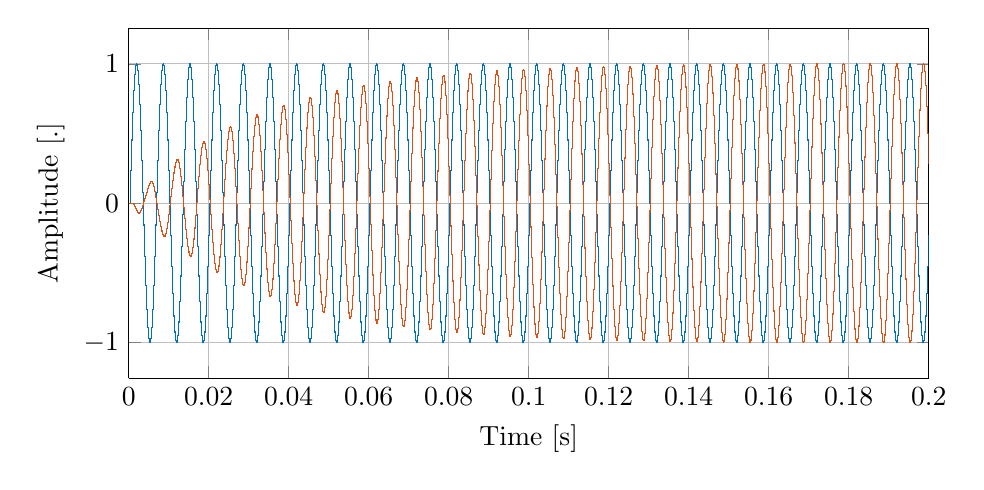
\begin{tikzpicture}

\begin{axis}[%
width=4in,
height=1.75in,
at={(0.27in,0.409in)},
scale only axis,
separate axis lines,
xmin=0,
xmax=0.20,
xlabel={Time [s]},
ylabel={{Amplitude [.]}},
xmajorgrids,
ymin=-1.25591,
ymax=1.25591,
ymajorgrids,
scaled y ticks = false,
y tick label style={/pgf/number format/fixed},
scaled x ticks = false,
x tick label style={/pgf/number format/fixed},
axis background/.style={fill=white}
]
\addplot[const plot,color=MATLABblue,solid,forget plot] plot table[row sep=crcr] {%
0	0\\
0.000125	0\\
0.00025	0\\
0.000375	0.117537397457838\\
0.0005	0.233445363855905\\
0.000625	0.346117057077493\\
0.00075	0.453990499739547\\
0.000875	0.555570233019602\\
0.001	0.649448048330184\\
0.001125	0.734322509435686\\
0.00125	0.809016994374947\\
0.001375	0.872496007072797\\
0.0015	0.923879532511287\\
0.001625	0.962455236453647\\
0.00175	0.987688340595138\\
0.001875	0.999229036240723\\
0.002	0.996917333733128\\
0.002125	0.980785280403231\\
0.00225	0.951056516295154\\
0.002375	0.908143173825081\\
0.0025	0.852640164354092\\
0.002625	0.785316930880745\\
0.00275	0.707106781186548\\
0.002875	0.619093949309834\\
0.003	0.522498564715949\\
0.003125	0.418659737537428\\
0.00325	0.309016994374947\\
0.003375	0.195090322016128\\
0.0035	0.0784590957278449\\
0.003625	-0.0392598157590686\\
0.00375	-0.156434465040231\\
0.003875	-0.271440449865074\\
0.004	-0.38268343236509\\
0.004125	-0.488621241496955\\
0.00425	-0.587785252292473\\
0.004375	-0.678800745532942\\
0.0045	-0.760405965600031\\
0.004625	-0.831469612302545\\
0.00475	-0.891006524188368\\
0.004875	-0.938191335922484\\
0.005	-0.972369920397677\\
0.005125	-0.993068456954926\\
0.00525	-1\\
0.005375	-0.993068456954927\\
0.0055	-0.972369920397677\\
0.005625	-0.938191335922484\\
0.00575	-0.891006524188368\\
0.005875	-0.831469612302545\\
0.006	-0.760405965600031\\
0.006125	-0.678800745532942\\
0.00625	-0.587785252292473\\
0.006375	-0.488621241496955\\
0.0065	-0.38268343236509\\
0.006625	-0.271440449865074\\
0.00675	-0.156434465040231\\
0.006875	-0.0392598157590686\\
0.007	0.078459095727845\\
0.007125	0.195090322016128\\
0.00725	0.309016994374948\\
0.007375	0.418659737537428\\
0.0075	0.522498564715949\\
0.007625	0.619093949309834\\
0.00775	0.707106781186548\\
0.007875	0.785316930880745\\
0.008	0.852640164354093\\
0.008125	0.908143173825081\\
0.00825	0.951056516295154\\
0.008375	0.98078528040323\\
0.0085	0.996917333733128\\
0.008625	0.999229036240723\\
0.00875	0.987688340595138\\
0.008875	0.962455236453648\\
0.009	0.923879532511287\\
0.009125	0.872496007072797\\
0.00925	0.809016994374948\\
0.009375	0.734322509435686\\
0.0095	0.649448048330184\\
0.009625	0.555570233019602\\
0.00975	0.453990499739547\\
0.009875	0.346117057077493\\
0.01	0.233445363855905\\
0.010125	0.117537397457838\\
0.01025	1.38777878078145e-17\\
0.010375	-0.117537397457838\\
0.0105	-0.233445363855905\\
0.010625	-0.346117057077493\\
0.01075	-0.453990499739547\\
0.010875	-0.555570233019602\\
0.011	-0.649448048330184\\
0.011125	-0.734322509435686\\
0.01125	-0.809016994374947\\
0.011375	-0.872496007072797\\
0.0115	-0.923879532511287\\
0.011625	-0.962455236453647\\
0.01175	-0.987688340595138\\
0.011875	-0.999229036240723\\
0.012	-0.996917333733128\\
0.012125	-0.980785280403231\\
0.01225	-0.951056516295154\\
0.012375	-0.908143173825081\\
0.0125	-0.852640164354092\\
0.012625	-0.785316930880745\\
0.01275	-0.707106781186548\\
0.012875	-0.619093949309834\\
0.013	-0.522498564715949\\
0.013125	-0.418659737537428\\
0.01325	-0.309016994374947\\
0.013375	-0.195090322016128\\
0.0135	-0.0784590957278449\\
0.013625	0.0392598157590686\\
0.01375	0.156434465040231\\
0.013875	0.271440449865074\\
0.014	0.38268343236509\\
0.014125	0.488621241496955\\
0.01425	0.587785252292473\\
0.014375	0.678800745532942\\
0.0145	0.760405965600031\\
0.014625	0.831469612302545\\
0.01475	0.891006524188368\\
0.014875	0.938191335922484\\
0.015	0.972369920397677\\
0.015125	0.993068456954926\\
0.01525	1\\
0.015375	0.993068456954927\\
0.0155	0.972369920397677\\
0.015625	0.938191335922484\\
0.01575	0.891006524188368\\
0.015875	0.831469612302545\\
0.016	0.760405965600031\\
0.016125	0.678800745532942\\
0.01625	0.587785252292473\\
0.016375	0.488621241496955\\
0.0165	0.38268343236509\\
0.016625	0.271440449865074\\
0.01675	0.156434465040231\\
0.016875	0.0392598157590686\\
0.017	-0.078459095727845\\
0.017125	-0.195090322016128\\
0.01725	-0.309016994374948\\
0.017375	-0.418659737537428\\
0.0175	-0.522498564715949\\
0.017625	-0.619093949309834\\
0.01775	-0.707106781186548\\
0.017875	-0.785316930880745\\
0.018	-0.852640164354093\\
0.018125	-0.908143173825081\\
0.01825	-0.951056516295154\\
0.018375	-0.98078528040323\\
0.0185	-0.996917333733128\\
0.018625	-0.999229036240723\\
0.01875	-0.987688340595138\\
0.018875	-0.962455236453648\\
0.019	-0.923879532511287\\
0.019125	-0.872496007072797\\
0.01925	-0.809016994374948\\
0.019375	-0.734322509435686\\
0.0195	-0.649448048330184\\
0.019625	-0.555570233019602\\
0.01975	-0.453990499739547\\
0.019875	-0.346117057077493\\
0.02	-0.233445363855905\\
0.020125	-0.117537397457838\\
0.02025	-1.38777878078145e-17\\
0.020375	0.117537397457838\\
0.0205	0.233445363855905\\
0.020625	0.346117057077493\\
0.02075	0.453990499739547\\
0.020875	0.555570233019602\\
0.021	0.649448048330184\\
0.021125	0.734322509435686\\
0.02125	0.809016994374947\\
0.021375	0.872496007072797\\
0.0215	0.923879532511287\\
0.021625	0.962455236453647\\
0.02175	0.987688340595138\\
0.021875	0.999229036240723\\
0.022	0.996917333733128\\
0.022125	0.980785280403231\\
0.02225	0.951056516295154\\
0.022375	0.908143173825081\\
0.0225	0.852640164354092\\
0.022625	0.785316930880745\\
0.02275	0.707106781186548\\
0.022875	0.619093949309834\\
0.023	0.522498564715949\\
0.023125	0.418659737537428\\
0.02325	0.309016994374947\\
0.023375	0.195090322016128\\
0.0235	0.0784590957278449\\
0.023625	-0.0392598157590686\\
0.02375	-0.156434465040231\\
0.023875	-0.271440449865074\\
0.024	-0.38268343236509\\
0.024125	-0.488621241496955\\
0.02425	-0.587785252292473\\
0.024375	-0.678800745532942\\
0.0245	-0.760405965600031\\
0.024625	-0.831469612302545\\
0.02475	-0.891006524188368\\
0.024875	-0.938191335922484\\
0.025	-0.972369920397677\\
0.025125	-0.993068456954926\\
0.02525	-1\\
0.025375	-0.993068456954927\\
0.0255	-0.972369920397677\\
0.025625	-0.938191335922484\\
0.02575	-0.891006524188368\\
0.025875	-0.831469612302545\\
0.026	-0.760405965600031\\
0.026125	-0.678800745532942\\
0.02625	-0.587785252292473\\
0.026375	-0.488621241496955\\
0.0265	-0.38268343236509\\
0.026625	-0.271440449865074\\
0.02675	-0.156434465040231\\
0.026875	-0.0392598157590686\\
0.027	0.078459095727845\\
0.027125	0.195090322016128\\
0.02725	0.309016994374948\\
0.027375	0.418659737537428\\
0.0275	0.522498564715949\\
0.027625	0.619093949309834\\
0.02775	0.707106781186548\\
0.027875	0.785316930880745\\
0.028	0.852640164354093\\
0.028125	0.908143173825081\\
0.02825	0.951056516295154\\
0.028375	0.98078528040323\\
0.0285	0.996917333733128\\
0.028625	0.999229036240723\\
0.02875	0.987688340595138\\
0.028875	0.962455236453648\\
0.029	0.923879532511287\\
0.029125	0.872496007072797\\
0.02925	0.809016994374948\\
0.029375	0.734322509435686\\
0.0295	0.649448048330184\\
0.029625	0.555570233019602\\
0.02975	0.453990499739547\\
0.029875	0.346117057077493\\
0.03	0.233445363855905\\
0.030125	0.117537397457838\\
0.03025	1.38777878078145e-17\\
0.030375	-0.117537397457838\\
0.0305	-0.233445363855905\\
0.030625	-0.346117057077493\\
0.03075	-0.453990499739547\\
0.030875	-0.555570233019602\\
0.031	-0.649448048330184\\
0.031125	-0.734322509435686\\
0.03125	-0.809016994374947\\
0.031375	-0.872496007072797\\
0.0315	-0.923879532511287\\
0.031625	-0.962455236453647\\
0.03175	-0.987688340595138\\
0.031875	-0.999229036240723\\
0.032	-0.996917333733128\\
0.032125	-0.980785280403231\\
0.03225	-0.951056516295154\\
0.032375	-0.908143173825081\\
0.0325	-0.852640164354092\\
0.032625	-0.785316930880745\\
0.03275	-0.707106781186548\\
0.032875	-0.619093949309834\\
0.033	-0.522498564715949\\
0.033125	-0.418659737537428\\
0.03325	-0.309016994374947\\
0.033375	-0.195090322016128\\
0.0335	-0.0784590957278449\\
0.033625	0.0392598157590686\\
0.03375	0.156434465040231\\
0.033875	0.271440449865074\\
0.034	0.38268343236509\\
0.034125	0.488621241496955\\
0.03425	0.587785252292473\\
0.034375	0.678800745532942\\
0.0345	0.760405965600031\\
0.034625	0.831469612302545\\
0.03475	0.891006524188368\\
0.034875	0.938191335922484\\
0.035	0.972369920397677\\
0.035125	0.993068456954926\\
0.03525	1\\
0.035375	0.993068456954927\\
0.0355	0.972369920397677\\
0.035625	0.938191335922484\\
0.03575	0.891006524188368\\
0.035875	0.831469612302545\\
0.036	0.760405965600031\\
0.036125	0.678800745532942\\
0.03625	0.587785252292473\\
0.036375	0.488621241496955\\
0.0365	0.38268343236509\\
0.036625	0.271440449865074\\
0.03675	0.156434465040231\\
0.036875	0.0392598157590686\\
0.037	-0.078459095727845\\
0.037125	-0.195090322016128\\
0.03725	-0.309016994374948\\
0.037375	-0.418659737537428\\
0.0375	-0.522498564715949\\
0.037625	-0.619093949309834\\
0.03775	-0.707106781186548\\
0.037875	-0.785316930880745\\
0.038	-0.852640164354093\\
0.038125	-0.908143173825081\\
0.03825	-0.951056516295154\\
0.038375	-0.98078528040323\\
0.0385	-0.996917333733128\\
0.038625	-0.999229036240723\\
0.03875	-0.987688340595138\\
0.038875	-0.962455236453648\\
0.039	-0.923879532511287\\
0.039125	-0.872496007072797\\
0.03925	-0.809016994374948\\
0.039375	-0.734322509435686\\
0.0395	-0.649448048330184\\
0.039625	-0.555570233019602\\
0.03975	-0.453990499739547\\
0.039875	-0.346117057077493\\
0.04	-0.233445363855905\\
0.040125	-0.117537397457838\\
0.04025	-1.38777878078145e-17\\
0.040375	0.117537397457838\\
0.0405	0.233445363855905\\
0.040625	0.346117057077493\\
0.04075	0.453990499739547\\
0.040875	0.555570233019602\\
0.041	0.649448048330184\\
0.041125	0.734322509435686\\
0.04125	0.809016994374947\\
0.041375	0.872496007072797\\
0.0415	0.923879532511287\\
0.041625	0.962455236453647\\
0.04175	0.987688340595138\\
0.041875	0.999229036240723\\
0.042	0.996917333733128\\
0.042125	0.980785280403231\\
0.04225	0.951056516295154\\
0.042375	0.908143173825081\\
0.0425	0.852640164354092\\
0.042625	0.785316930880745\\
0.04275	0.707106781186548\\
0.042875	0.619093949309834\\
0.043	0.522498564715949\\
0.043125	0.418659737537428\\
0.04325	0.309016994374947\\
0.043375	0.195090322016128\\
0.0435	0.0784590957278449\\
0.043625	-0.0392598157590686\\
0.04375	-0.156434465040231\\
0.043875	-0.271440449865074\\
0.044	-0.38268343236509\\
0.044125	-0.488621241496955\\
0.04425	-0.587785252292473\\
0.044375	-0.678800745532942\\
0.0445	-0.760405965600031\\
0.044625	-0.831469612302545\\
0.04475	-0.891006524188368\\
0.044875	-0.938191335922484\\
0.045	-0.972369920397677\\
0.045125	-0.993068456954926\\
0.04525	-1\\
0.045375	-0.993068456954927\\
0.0455	-0.972369920397677\\
0.045625	-0.938191335922484\\
0.04575	-0.891006524188368\\
0.045875	-0.831469612302545\\
0.046	-0.760405965600031\\
0.046125	-0.678800745532942\\
0.04625	-0.587785252292473\\
0.046375	-0.488621241496955\\
0.0465	-0.38268343236509\\
0.046625	-0.271440449865074\\
0.04675	-0.156434465040231\\
0.046875	-0.0392598157590686\\
0.047	0.078459095727845\\
0.047125	0.195090322016128\\
0.04725	0.309016994374948\\
0.047375	0.418659737537428\\
0.0475	0.522498564715949\\
0.047625	0.619093949309834\\
0.04775	0.707106781186548\\
0.047875	0.785316930880745\\
0.048	0.852640164354093\\
0.048125	0.908143173825081\\
0.04825	0.951056516295154\\
0.048375	0.98078528040323\\
0.0485	0.996917333733128\\
0.048625	0.999229036240723\\
0.04875	0.987688340595138\\
0.048875	0.962455236453648\\
0.049	0.923879532511287\\
0.049125	0.872496007072797\\
0.04925	0.809016994374948\\
0.049375	0.734322509435686\\
0.0495	0.649448048330184\\
0.049625	0.555570233019602\\
0.04975	0.453990499739547\\
0.049875	0.346117057077493\\
0.05	0.233445363855905\\
0.050125	0.117537397457838\\
0.05025	1.38777878078145e-17\\
0.050375	-0.117537397457838\\
0.0505	-0.233445363855905\\
0.050625	-0.346117057077493\\
0.05075	-0.453990499739547\\
0.050875	-0.555570233019602\\
0.051	-0.649448048330184\\
0.051125	-0.734322509435686\\
0.05125	-0.809016994374947\\
0.051375	-0.872496007072797\\
0.0515	-0.923879532511287\\
0.051625	-0.962455236453647\\
0.05175	-0.987688340595138\\
0.051875	-0.999229036240723\\
0.052	-0.996917333733128\\
0.052125	-0.980785280403231\\
0.05225	-0.951056516295154\\
0.052375	-0.908143173825081\\
0.0525	-0.852640164354092\\
0.052625	-0.785316930880745\\
0.05275	-0.707106781186548\\
0.052875	-0.619093949309834\\
0.053	-0.522498564715949\\
0.053125	-0.418659737537428\\
0.05325	-0.309016994374947\\
0.053375	-0.195090322016128\\
0.0535	-0.0784590957278449\\
0.053625	0.0392598157590686\\
0.05375	0.156434465040231\\
0.053875	0.271440449865074\\
0.054	0.38268343236509\\
0.054125	0.488621241496955\\
0.05425	0.587785252292473\\
0.054375	0.678800745532942\\
0.0545	0.760405965600031\\
0.054625	0.831469612302545\\
0.05475	0.891006524188368\\
0.054875	0.938191335922484\\
0.055	0.972369920397677\\
0.055125	0.993068456954926\\
0.05525	1\\
0.055375	0.993068456954927\\
0.0555	0.972369920397677\\
0.055625	0.938191335922484\\
0.05575	0.891006524188368\\
0.055875	0.831469612302545\\
0.056	0.760405965600031\\
0.056125	0.678800745532942\\
0.05625	0.587785252292473\\
0.056375	0.488621241496955\\
0.0565	0.38268343236509\\
0.056625	0.271440449865074\\
0.05675	0.156434465040231\\
0.056875	0.0392598157590686\\
0.057	-0.078459095727845\\
0.057125	-0.195090322016128\\
0.05725	-0.309016994374948\\
0.057375	-0.418659737537428\\
0.0575	-0.522498564715949\\
0.057625	-0.619093949309834\\
0.05775	-0.707106781186548\\
0.057875	-0.785316930880745\\
0.058	-0.852640164354093\\
0.058125	-0.908143173825081\\
0.05825	-0.951056516295154\\
0.058375	-0.98078528040323\\
0.0585	-0.996917333733128\\
0.058625	-0.999229036240723\\
0.05875	-0.987688340595138\\
0.058875	-0.962455236453648\\
0.059	-0.923879532511287\\
0.059125	-0.872496007072797\\
0.05925	-0.809016994374948\\
0.059375	-0.734322509435686\\
0.0595	-0.649448048330184\\
0.059625	-0.555570233019602\\
0.05975	-0.453990499739547\\
0.059875	-0.346117057077493\\
0.06	-0.233445363855905\\
0.060125	-0.117537397457838\\
0.06025	-1.38777878078145e-17\\
0.060375	0.117537397457838\\
0.0605	0.233445363855905\\
0.060625	0.346117057077493\\
0.06075	0.453990499739547\\
0.060875	0.555570233019602\\
0.061	0.649448048330184\\
0.061125	0.734322509435686\\
0.06125	0.809016994374947\\
0.061375	0.872496007072797\\
0.0615	0.923879532511287\\
0.061625	0.962455236453647\\
0.06175	0.987688340595138\\
0.061875	0.999229036240723\\
0.062	0.996917333733128\\
0.062125	0.980785280403231\\
0.06225	0.951056516295154\\
0.062375	0.908143173825081\\
0.0625	0.852640164354092\\
0.062625	0.785316930880745\\
0.06275	0.707106781186548\\
0.062875	0.619093949309834\\
0.063	0.522498564715949\\
0.063125	0.418659737537428\\
0.06325	0.309016994374947\\
0.063375	0.195090322016128\\
0.0635	0.0784590957278449\\
0.063625	-0.0392598157590686\\
0.06375	-0.156434465040231\\
0.063875	-0.271440449865074\\
0.064	-0.38268343236509\\
0.064125	-0.488621241496955\\
0.06425	-0.587785252292473\\
0.064375	-0.678800745532942\\
0.0645	-0.760405965600031\\
0.064625	-0.831469612302545\\
0.06475	-0.891006524188368\\
0.064875	-0.938191335922484\\
0.065	-0.972369920397677\\
0.065125	-0.993068456954926\\
0.06525	-1\\
0.065375	-0.993068456954927\\
0.0655	-0.972369920397677\\
0.065625	-0.938191335922484\\
0.06575	-0.891006524188368\\
0.065875	-0.831469612302545\\
0.066	-0.760405965600031\\
0.066125	-0.678800745532942\\
0.06625	-0.587785252292473\\
0.066375	-0.488621241496955\\
0.0665	-0.38268343236509\\
0.066625	-0.271440449865074\\
0.06675	-0.156434465040231\\
0.066875	-0.0392598157590686\\
0.067	0.078459095727845\\
0.067125	0.195090322016128\\
0.06725	0.309016994374948\\
0.067375	0.418659737537428\\
0.0675	0.522498564715949\\
0.067625	0.619093949309834\\
0.06775	0.707106781186548\\
0.067875	0.785316930880745\\
0.068	0.852640164354093\\
0.068125	0.908143173825081\\
0.06825	0.951056516295154\\
0.068375	0.98078528040323\\
0.0685	0.996917333733128\\
0.068625	0.999229036240723\\
0.06875	0.987688340595138\\
0.068875	0.962455236453648\\
0.069	0.923879532511287\\
0.069125	0.872496007072797\\
0.06925	0.809016994374948\\
0.069375	0.734322509435686\\
0.0695	0.649448048330184\\
0.069625	0.555570233019602\\
0.06975	0.453990499739547\\
0.069875	0.346117057077493\\
0.07	0.233445363855905\\
0.070125	0.117537397457838\\
0.07025	1.38777878078145e-17\\
0.070375	-0.117537397457838\\
0.0705	-0.233445363855905\\
0.070625	-0.346117057077493\\
0.07075	-0.453990499739547\\
0.070875	-0.555570233019602\\
0.071	-0.649448048330184\\
0.071125	-0.734322509435686\\
0.07125	-0.809016994374947\\
0.071375	-0.872496007072797\\
0.0715	-0.923879532511287\\
0.071625	-0.962455236453647\\
0.07175	-0.987688340595138\\
0.071875	-0.999229036240723\\
0.072	-0.996917333733128\\
0.072125	-0.980785280403231\\
0.07225	-0.951056516295154\\
0.072375	-0.908143173825081\\
0.0725	-0.852640164354092\\
0.072625	-0.785316930880745\\
0.07275	-0.707106781186548\\
0.072875	-0.619093949309834\\
0.073	-0.522498564715949\\
0.073125	-0.418659737537428\\
0.07325	-0.309016994374947\\
0.073375	-0.195090322016128\\
0.0735	-0.0784590957278449\\
0.073625	0.0392598157590686\\
0.07375	0.156434465040231\\
0.073875	0.271440449865074\\
0.074	0.38268343236509\\
0.074125	0.488621241496955\\
0.07425	0.587785252292473\\
0.074375	0.678800745532942\\
0.0745	0.760405965600031\\
0.074625	0.831469612302545\\
0.07475	0.891006524188368\\
0.074875	0.938191335922484\\
0.075	0.972369920397677\\
0.075125	0.993068456954926\\
0.07525	1\\
0.075375	0.993068456954927\\
0.0755	0.972369920397677\\
0.075625	0.938191335922484\\
0.07575	0.891006524188368\\
0.075875	0.831469612302545\\
0.076	0.760405965600031\\
0.076125	0.678800745532942\\
0.07625	0.587785252292473\\
0.076375	0.488621241496955\\
0.0765	0.38268343236509\\
0.076625	0.271440449865074\\
0.07675	0.156434465040231\\
0.076875	0.0392598157590686\\
0.077	-0.078459095727845\\
0.077125	-0.195090322016128\\
0.07725	-0.309016994374948\\
0.077375	-0.418659737537428\\
0.0775	-0.522498564715949\\
0.077625	-0.619093949309834\\
0.07775	-0.707106781186548\\
0.077875	-0.785316930880745\\
0.078	-0.852640164354093\\
0.078125	-0.908143173825081\\
0.07825	-0.951056516295154\\
0.078375	-0.98078528040323\\
0.0785	-0.996917333733128\\
0.078625	-0.999229036240723\\
0.07875	-0.987688340595138\\
0.078875	-0.962455236453648\\
0.079	-0.923879532511287\\
0.079125	-0.872496007072797\\
0.07925	-0.809016994374948\\
0.079375	-0.734322509435686\\
0.0795	-0.649448048330184\\
0.079625	-0.555570233019602\\
0.07975	-0.453990499739547\\
0.079875	-0.346117057077493\\
0.08	-0.233445363855905\\
0.080125	-0.117537397457838\\
0.08025	-1.38777878078145e-17\\
0.080375	0.117537397457838\\
0.0805	0.233445363855905\\
0.080625	0.346117057077493\\
0.08075	0.453990499739547\\
0.080875	0.555570233019602\\
0.081	0.649448048330184\\
0.081125	0.734322509435686\\
0.08125	0.809016994374947\\
0.081375	0.872496007072797\\
0.0815	0.923879532511287\\
0.081625	0.962455236453647\\
0.08175	0.987688340595138\\
0.081875	0.999229036240723\\
0.082	0.996917333733128\\
0.082125	0.980785280403231\\
0.08225	0.951056516295154\\
0.082375	0.908143173825081\\
0.0825	0.852640164354092\\
0.082625	0.785316930880745\\
0.08275	0.707106781186548\\
0.082875	0.619093949309834\\
0.083	0.522498564715949\\
0.083125	0.418659737537428\\
0.08325	0.309016994374947\\
0.083375	0.195090322016128\\
0.0835	0.0784590957278449\\
0.083625	-0.0392598157590686\\
0.08375	-0.156434465040231\\
0.083875	-0.271440449865074\\
0.084	-0.38268343236509\\
0.084125	-0.488621241496955\\
0.08425	-0.587785252292473\\
0.084375	-0.678800745532942\\
0.0845	-0.760405965600031\\
0.084625	-0.831469612302545\\
0.08475	-0.891006524188368\\
0.084875	-0.938191335922484\\
0.085	-0.972369920397677\\
0.085125	-0.993068456954926\\
0.08525	-1\\
0.085375	-0.993068456954927\\
0.0855	-0.972369920397677\\
0.085625	-0.938191335922484\\
0.08575	-0.891006524188368\\
0.085875	-0.831469612302545\\
0.086	-0.760405965600031\\
0.086125	-0.678800745532942\\
0.08625	-0.587785252292473\\
0.086375	-0.488621241496955\\
0.0865	-0.38268343236509\\
0.086625	-0.271440449865074\\
0.08675	-0.156434465040231\\
0.086875	-0.0392598157590686\\
0.087	0.078459095727845\\
0.087125	0.195090322016128\\
0.08725	0.309016994374948\\
0.087375	0.418659737537428\\
0.0875	0.522498564715949\\
0.087625	0.619093949309834\\
0.08775	0.707106781186548\\
0.087875	0.785316930880745\\
0.088	0.852640164354093\\
0.088125	0.908143173825081\\
0.08825	0.951056516295154\\
0.088375	0.98078528040323\\
0.0885	0.996917333733128\\
0.088625	0.999229036240723\\
0.08875	0.987688340595138\\
0.088875	0.962455236453648\\
0.089	0.923879532511287\\
0.089125	0.872496007072797\\
0.08925	0.809016994374948\\
0.089375	0.734322509435686\\
0.0895	0.649448048330184\\
0.089625	0.555570233019602\\
0.08975	0.453990499739547\\
0.089875	0.346117057077493\\
0.09	0.233445363855905\\
0.090125	0.117537397457838\\
0.09025	1.38777878078145e-17\\
0.090375	-0.117537397457838\\
0.0905	-0.233445363855905\\
0.090625	-0.346117057077493\\
0.09075	-0.453990499739547\\
0.090875	-0.555570233019602\\
0.091	-0.649448048330184\\
0.091125	-0.734322509435686\\
0.09125	-0.809016994374947\\
0.091375	-0.872496007072797\\
0.0915	-0.923879532511287\\
0.091625	-0.962455236453647\\
0.09175	-0.987688340595138\\
0.091875	-0.999229036240723\\
0.092	-0.996917333733128\\
0.092125	-0.980785280403231\\
0.09225	-0.951056516295154\\
0.092375	-0.908143173825081\\
0.0925	-0.852640164354092\\
0.092625	-0.785316930880745\\
0.09275	-0.707106781186548\\
0.092875	-0.619093949309834\\
0.093	-0.522498564715949\\
0.093125	-0.418659737537428\\
0.09325	-0.309016994374947\\
0.093375	-0.195090322016128\\
0.0935	-0.0784590957278449\\
0.093625	0.0392598157590686\\
0.09375	0.156434465040231\\
0.093875	0.271440449865074\\
0.094	0.38268343236509\\
0.094125	0.488621241496955\\
0.09425	0.587785252292473\\
0.094375	0.678800745532942\\
0.0945	0.760405965600031\\
0.094625	0.831469612302545\\
0.09475	0.891006524188368\\
0.094875	0.938191335922484\\
0.095	0.972369920397677\\
0.095125	0.993068456954926\\
0.09525	1\\
0.095375	0.993068456954927\\
0.0955	0.972369920397677\\
0.095625	0.938191335922484\\
0.09575	0.891006524188368\\
0.095875	0.831469612302545\\
0.096	0.760405965600031\\
0.096125	0.678800745532942\\
0.09625	0.587785252292473\\
0.096375	0.488621241496955\\
0.0965	0.38268343236509\\
0.096625	0.271440449865074\\
0.09675	0.156434465040231\\
0.096875	0.0392598157590686\\
0.097	-0.078459095727845\\
0.097125	-0.195090322016128\\
0.09725	-0.309016994374948\\
0.097375	-0.418659737537428\\
0.0975	-0.522498564715949\\
0.097625	-0.619093949309834\\
0.09775	-0.707106781186548\\
0.097875	-0.785316930880745\\
0.098	-0.852640164354093\\
0.098125	-0.908143173825081\\
0.09825	-0.951056516295154\\
0.098375	-0.98078528040323\\
0.0985	-0.996917333733128\\
0.098625	-0.999229036240723\\
0.09875	-0.987688340595138\\
0.098875	-0.962455236453648\\
0.099	-0.923879532511287\\
0.099125	-0.872496007072797\\
0.09925	-0.809016994374948\\
0.099375	-0.734322509435686\\
0.0995	-0.649448048330184\\
0.099625	-0.555570233019602\\
0.09975	-0.453990499739547\\
0.099875	-0.346117057077493\\
0.1	-0.233445363855905\\
0.100125	-0.117537397457838\\
0.10025	-1.38777878078145e-17\\
0.100375	0.117537397457838\\
0.1005	0.233445363855905\\
0.100625	0.346117057077493\\
0.10075	0.453990499739547\\
0.100875	0.555570233019602\\
0.101	0.649448048330184\\
0.101125	0.734322509435686\\
0.10125	0.809016994374947\\
0.101375	0.872496007072797\\
0.1015	0.923879532511287\\
0.101625	0.962455236453647\\
0.10175	0.987688340595138\\
0.101875	0.999229036240723\\
0.102	0.996917333733128\\
0.102125	0.980785280403231\\
0.10225	0.951056516295154\\
0.102375	0.908143173825081\\
0.1025	0.852640164354092\\
0.102625	0.785316930880745\\
0.10275	0.707106781186548\\
0.102875	0.619093949309834\\
0.103	0.522498564715949\\
0.103125	0.418659737537428\\
0.10325	0.309016994374947\\
0.103375	0.195090322016128\\
0.1035	0.0784590957278449\\
0.103625	-0.0392598157590686\\
0.10375	-0.156434465040231\\
0.103875	-0.271440449865074\\
0.104	-0.38268343236509\\
0.104125	-0.488621241496955\\
0.10425	-0.587785252292473\\
0.104375	-0.678800745532942\\
0.1045	-0.760405965600031\\
0.104625	-0.831469612302545\\
0.10475	-0.891006524188368\\
0.104875	-0.938191335922484\\
0.105	-0.972369920397677\\
0.105125	-0.993068456954926\\
0.10525	-1\\
0.105375	-0.993068456954927\\
0.1055	-0.972369920397677\\
0.105625	-0.938191335922484\\
0.10575	-0.891006524188368\\
0.105875	-0.831469612302545\\
0.106	-0.760405965600031\\
0.106125	-0.678800745532942\\
0.10625	-0.587785252292473\\
0.106375	-0.488621241496955\\
0.1065	-0.38268343236509\\
0.106625	-0.271440449865074\\
0.10675	-0.156434465040231\\
0.106875	-0.0392598157590686\\
0.107	0.078459095727845\\
0.107125	0.195090322016128\\
0.10725	0.309016994374948\\
0.107375	0.418659737537428\\
0.1075	0.522498564715949\\
0.107625	0.619093949309834\\
0.10775	0.707106781186548\\
0.107875	0.785316930880745\\
0.108	0.852640164354093\\
0.108125	0.908143173825081\\
0.10825	0.951056516295154\\
0.108375	0.98078528040323\\
0.1085	0.996917333733128\\
0.108625	0.999229036240723\\
0.10875	0.987688340595138\\
0.108875	0.962455236453648\\
0.109	0.923879532511287\\
0.109125	0.872496007072797\\
0.10925	0.809016994374948\\
0.109375	0.734322509435686\\
0.1095	0.649448048330184\\
0.109625	0.555570233019602\\
0.10975	0.453990499739547\\
0.109875	0.346117057077493\\
0.11	0.233445363855905\\
0.110125	0.117537397457838\\
0.11025	1.38777878078145e-17\\
0.110375	-0.117537397457838\\
0.1105	-0.233445363855905\\
0.110625	-0.346117057077493\\
0.11075	-0.453990499739547\\
0.110875	-0.555570233019602\\
0.111	-0.649448048330184\\
0.111125	-0.734322509435686\\
0.11125	-0.809016994374947\\
0.111375	-0.872496007072797\\
0.1115	-0.923879532511287\\
0.111625	-0.962455236453647\\
0.11175	-0.987688340595138\\
0.111875	-0.999229036240723\\
0.112	-0.996917333733128\\
0.112125	-0.980785280403231\\
0.11225	-0.951056516295154\\
0.112375	-0.908143173825081\\
0.1125	-0.852640164354092\\
0.112625	-0.785316930880745\\
0.11275	-0.707106781186548\\
0.112875	-0.619093949309834\\
0.113	-0.522498564715949\\
0.113125	-0.418659737537428\\
0.11325	-0.309016994374947\\
0.113375	-0.195090322016128\\
0.1135	-0.0784590957278449\\
0.113625	0.0392598157590686\\
0.11375	0.156434465040231\\
0.113875	0.271440449865074\\
0.114	0.38268343236509\\
0.114125	0.488621241496955\\
0.11425	0.587785252292473\\
0.114375	0.678800745532942\\
0.1145	0.760405965600031\\
0.114625	0.831469612302545\\
0.11475	0.891006524188368\\
0.114875	0.938191335922484\\
0.115	0.972369920397677\\
0.115125	0.993068456954926\\
0.11525	1\\
0.115375	0.993068456954927\\
0.1155	0.972369920397677\\
0.115625	0.938191335922484\\
0.11575	0.891006524188368\\
0.115875	0.831469612302545\\
0.116	0.760405965600031\\
0.116125	0.678800745532942\\
0.11625	0.587785252292473\\
0.116375	0.488621241496955\\
0.1165	0.38268343236509\\
0.116625	0.271440449865074\\
0.11675	0.156434465040231\\
0.116875	0.0392598157590686\\
0.117	-0.078459095727845\\
0.117125	-0.195090322016128\\
0.11725	-0.309016994374948\\
0.117375	-0.418659737537428\\
0.1175	-0.522498564715949\\
0.117625	-0.619093949309834\\
0.11775	-0.707106781186548\\
0.117875	-0.785316930880745\\
0.118	-0.852640164354093\\
0.118125	-0.908143173825081\\
0.11825	-0.951056516295154\\
0.118375	-0.98078528040323\\
0.1185	-0.996917333733128\\
0.118625	-0.999229036240723\\
0.11875	-0.987688340595138\\
0.118875	-0.962455236453648\\
0.119	-0.923879532511287\\
0.119125	-0.872496007072797\\
0.11925	-0.809016994374948\\
0.119375	-0.734322509435686\\
0.1195	-0.649448048330184\\
0.119625	-0.555570233019602\\
0.11975	-0.453990499739547\\
0.119875	-0.346117057077493\\
0.12	-0.233445363855905\\
0.120125	-0.117537397457838\\
0.12025	-1.38777878078145e-17\\
0.120375	0.117537397457838\\
0.1205	0.233445363855905\\
0.120625	0.346117057077493\\
0.12075	0.453990499739547\\
0.120875	0.555570233019602\\
0.121	0.649448048330184\\
0.121125	0.734322509435686\\
0.12125	0.809016994374947\\
0.121375	0.872496007072797\\
0.1215	0.923879532511287\\
0.121625	0.962455236453647\\
0.12175	0.987688340595138\\
0.121875	0.999229036240723\\
0.122	0.996917333733128\\
0.122125	0.980785280403231\\
0.12225	0.951056516295154\\
0.122375	0.908143173825081\\
0.1225	0.852640164354092\\
0.122625	0.785316930880745\\
0.12275	0.707106781186548\\
0.122875	0.619093949309834\\
0.123	0.522498564715949\\
0.123125	0.418659737537428\\
0.12325	0.309016994374947\\
0.123375	0.195090322016128\\
0.1235	0.0784590957278449\\
0.123625	-0.0392598157590686\\
0.12375	-0.156434465040231\\
0.123875	-0.271440449865074\\
0.124	-0.38268343236509\\
0.124125	-0.488621241496955\\
0.12425	-0.587785252292473\\
0.124375	-0.678800745532942\\
0.1245	-0.760405965600031\\
0.124625	-0.831469612302545\\
0.12475	-0.891006524188368\\
0.124875	-0.938191335922484\\
0.125	-0.972369920397677\\
0.125125	-0.993068456954926\\
0.12525	-1\\
0.125375	-0.993068456954927\\
0.1255	-0.972369920397677\\
0.125625	-0.938191335922484\\
0.12575	-0.891006524188368\\
0.125875	-0.831469612302545\\
0.126	-0.760405965600031\\
0.126125	-0.678800745532942\\
0.12625	-0.587785252292473\\
0.126375	-0.488621241496955\\
0.1265	-0.38268343236509\\
0.126625	-0.271440449865074\\
0.12675	-0.156434465040231\\
0.126875	-0.0392598157590686\\
0.127	0.078459095727845\\
0.127125	0.195090322016128\\
0.12725	0.309016994374948\\
0.127375	0.418659737537428\\
0.1275	0.522498564715949\\
0.127625	0.619093949309834\\
0.12775	0.707106781186548\\
0.127875	0.785316930880745\\
0.128	0.852640164354093\\
0.128125	0.908143173825081\\
0.12825	0.951056516295154\\
0.128375	0.98078528040323\\
0.1285	0.996917333733128\\
0.128625	0.999229036240723\\
0.12875	0.987688340595138\\
0.128875	0.962455236453648\\
0.129	0.923879532511287\\
0.129125	0.872496007072797\\
0.12925	0.809016994374948\\
0.129375	0.734322509435686\\
0.1295	0.649448048330184\\
0.129625	0.555570233019602\\
0.12975	0.453990499739547\\
0.129875	0.346117057077493\\
0.13	0.233445363855905\\
0.130125	0.117537397457838\\
0.13025	1.38777878078145e-17\\
0.130375	-0.117537397457838\\
0.1305	-0.233445363855905\\
0.130625	-0.346117057077493\\
0.13075	-0.453990499739547\\
0.130875	-0.555570233019602\\
0.131	-0.649448048330184\\
0.131125	-0.734322509435686\\
0.13125	-0.809016994374947\\
0.131375	-0.872496007072797\\
0.1315	-0.923879532511287\\
0.131625	-0.962455236453647\\
0.13175	-0.987688340595138\\
0.131875	-0.999229036240723\\
0.132	-0.996917333733128\\
0.132125	-0.980785280403231\\
0.13225	-0.951056516295154\\
0.132375	-0.908143173825081\\
0.1325	-0.852640164354092\\
0.132625	-0.785316930880745\\
0.13275	-0.707106781186548\\
0.132875	-0.619093949309834\\
0.133	-0.522498564715949\\
0.133125	-0.418659737537428\\
0.13325	-0.309016994374947\\
0.133375	-0.195090322016128\\
0.1335	-0.0784590957278449\\
0.133625	0.0392598157590686\\
0.13375	0.156434465040231\\
0.133875	0.271440449865074\\
0.134	0.38268343236509\\
0.134125	0.488621241496955\\
0.13425	0.587785252292473\\
0.134375	0.678800745532942\\
0.1345	0.760405965600031\\
0.134625	0.831469612302545\\
0.13475	0.891006524188368\\
0.134875	0.938191335922484\\
0.135	0.972369920397677\\
0.135125	0.993068456954926\\
0.13525	1\\
0.135375	0.993068456954927\\
0.1355	0.972369920397677\\
0.135625	0.938191335922484\\
0.13575	0.891006524188368\\
0.135875	0.831469612302545\\
0.136	0.760405965600031\\
0.136125	0.678800745532942\\
0.13625	0.587785252292473\\
0.136375	0.488621241496955\\
0.1365	0.38268343236509\\
0.136625	0.271440449865074\\
0.13675	0.156434465040231\\
0.136875	0.0392598157590686\\
0.137	-0.078459095727845\\
0.137125	-0.195090322016128\\
0.13725	-0.309016994374948\\
0.137375	-0.418659737537428\\
0.1375	-0.522498564715949\\
0.137625	-0.619093949309834\\
0.13775	-0.707106781186548\\
0.137875	-0.785316930880745\\
0.138	-0.852640164354093\\
0.138125	-0.908143173825081\\
0.13825	-0.951056516295154\\
0.138375	-0.98078528040323\\
0.1385	-0.996917333733128\\
0.138625	-0.999229036240723\\
0.13875	-0.987688340595138\\
0.138875	-0.962455236453648\\
0.139	-0.923879532511287\\
0.139125	-0.872496007072797\\
0.13925	-0.809016994374948\\
0.139375	-0.734322509435686\\
0.1395	-0.649448048330184\\
0.139625	-0.555570233019602\\
0.13975	-0.453990499739547\\
0.139875	-0.346117057077493\\
0.14	-0.233445363855905\\
0.140125	-0.117537397457838\\
0.14025	-1.38777878078145e-17\\
0.140375	0.117537397457838\\
0.1405	0.233445363855905\\
0.140625	0.346117057077493\\
0.14075	0.453990499739547\\
0.140875	0.555570233019602\\
0.141	0.649448048330184\\
0.141125	0.734322509435686\\
0.14125	0.809016994374947\\
0.141375	0.872496007072797\\
0.1415	0.923879532511287\\
0.141625	0.962455236453647\\
0.14175	0.987688340595138\\
0.141875	0.999229036240723\\
0.142	0.996917333733128\\
0.142125	0.980785280403231\\
0.14225	0.951056516295154\\
0.142375	0.908143173825081\\
0.1425	0.852640164354092\\
0.142625	0.785316930880745\\
0.14275	0.707106781186548\\
0.142875	0.619093949309834\\
0.143	0.522498564715949\\
0.143125	0.418659737537428\\
0.14325	0.309016994374947\\
0.143375	0.195090322016128\\
0.1435	0.0784590957278449\\
0.143625	-0.0392598157590686\\
0.14375	-0.156434465040231\\
0.143875	-0.271440449865074\\
0.144	-0.38268343236509\\
0.144125	-0.488621241496955\\
0.14425	-0.587785252292473\\
0.144375	-0.678800745532942\\
0.1445	-0.760405965600031\\
0.144625	-0.831469612302545\\
0.14475	-0.891006524188368\\
0.144875	-0.938191335922484\\
0.145	-0.972369920397677\\
0.145125	-0.993068456954926\\
0.14525	-1\\
0.145375	-0.993068456954927\\
0.1455	-0.972369920397677\\
0.145625	-0.938191335922484\\
0.14575	-0.891006524188368\\
0.145875	-0.831469612302545\\
0.146	-0.760405965600031\\
0.146125	-0.678800745532942\\
0.14625	-0.587785252292473\\
0.146375	-0.488621241496955\\
0.1465	-0.38268343236509\\
0.146625	-0.271440449865074\\
0.14675	-0.156434465040231\\
0.146875	-0.0392598157590686\\
0.147	0.078459095727845\\
0.147125	0.195090322016128\\
0.14725	0.309016994374948\\
0.147375	0.418659737537428\\
0.1475	0.522498564715949\\
0.147625	0.619093949309834\\
0.14775	0.707106781186548\\
0.147875	0.785316930880745\\
0.148	0.852640164354093\\
0.148125	0.908143173825081\\
0.14825	0.951056516295154\\
0.148375	0.98078528040323\\
0.1485	0.996917333733128\\
0.148625	0.999229036240723\\
0.14875	0.987688340595138\\
0.148875	0.962455236453648\\
0.149	0.923879532511287\\
0.149125	0.872496007072797\\
0.14925	0.809016994374948\\
0.149375	0.734322509435686\\
0.1495	0.649448048330184\\
0.149625	0.555570233019602\\
0.14975	0.453990499739547\\
0.149875	0.346117057077493\\
0.15	0.233445363855905\\
0.150125	0.117537397457838\\
0.15025	1.38777878078145e-17\\
0.150375	-0.117537397457838\\
0.1505	-0.233445363855905\\
0.150625	-0.346117057077493\\
0.15075	-0.453990499739547\\
0.150875	-0.555570233019602\\
0.151	-0.649448048330184\\
0.151125	-0.734322509435686\\
0.15125	-0.809016994374947\\
0.151375	-0.872496007072797\\
0.1515	-0.923879532511287\\
0.151625	-0.962455236453647\\
0.15175	-0.987688340595138\\
0.151875	-0.999229036240723\\
0.152	-0.996917333733128\\
0.152125	-0.980785280403231\\
0.15225	-0.951056516295154\\
0.152375	-0.908143173825081\\
0.1525	-0.852640164354092\\
0.152625	-0.785316930880745\\
0.15275	-0.707106781186548\\
0.152875	-0.619093949309834\\
0.153	-0.522498564715949\\
0.153125	-0.418659737537428\\
0.15325	-0.309016994374947\\
0.153375	-0.195090322016128\\
0.1535	-0.0784590957278449\\
0.153625	0.0392598157590686\\
0.15375	0.156434465040231\\
0.153875	0.271440449865074\\
0.154	0.38268343236509\\
0.154125	0.488621241496955\\
0.15425	0.587785252292473\\
0.154375	0.678800745532942\\
0.1545	0.760405965600031\\
0.154625	0.831469612302545\\
0.15475	0.891006524188368\\
0.154875	0.938191335922484\\
0.155	0.972369920397677\\
0.155125	0.993068456954926\\
0.15525	1\\
0.155375	0.993068456954927\\
0.1555	0.972369920397677\\
0.155625	0.938191335922484\\
0.15575	0.891006524188368\\
0.155875	0.831469612302545\\
0.156	0.760405965600031\\
0.156125	0.678800745532942\\
0.15625	0.587785252292473\\
0.156375	0.488621241496955\\
0.1565	0.38268343236509\\
0.156625	0.271440449865074\\
0.15675	0.156434465040231\\
0.156875	0.0392598157590686\\
0.157	-0.078459095727845\\
0.157125	-0.195090322016128\\
0.15725	-0.309016994374948\\
0.157375	-0.418659737537428\\
0.1575	-0.522498564715949\\
0.157625	-0.619093949309834\\
0.15775	-0.707106781186548\\
0.157875	-0.785316930880745\\
0.158	-0.852640164354093\\
0.158125	-0.908143173825081\\
0.15825	-0.951056516295154\\
0.158375	-0.98078528040323\\
0.1585	-0.996917333733128\\
0.158625	-0.999229036240723\\
0.15875	-0.987688340595138\\
0.158875	-0.962455236453648\\
0.159	-0.923879532511287\\
0.159125	-0.872496007072797\\
0.15925	-0.809016994374948\\
0.159375	-0.734322509435686\\
0.1595	-0.649448048330184\\
0.159625	-0.555570233019602\\
0.15975	-0.453990499739547\\
0.159875	-0.346117057077493\\
0.16	-0.233445363855905\\
0.160125	-0.117537397457838\\
0.16025	-1.38777878078145e-17\\
0.160375	0.117537397457838\\
0.1605	0.233445363855905\\
0.160625	0.346117057077493\\
0.16075	0.453990499739547\\
0.160875	0.555570233019602\\
0.161	0.649448048330184\\
0.161125	0.734322509435686\\
0.16125	0.809016994374947\\
0.161375	0.872496007072797\\
0.1615	0.923879532511287\\
0.161625	0.962455236453647\\
0.16175	0.987688340595138\\
0.161875	0.999229036240723\\
0.162	0.996917333733128\\
0.162125	0.980785280403231\\
0.16225	0.951056516295154\\
0.162375	0.908143173825081\\
0.1625	0.852640164354092\\
0.162625	0.785316930880745\\
0.16275	0.707106781186548\\
0.162875	0.619093949309834\\
0.163	0.522498564715949\\
0.163125	0.418659737537428\\
0.16325	0.309016994374947\\
0.163375	0.195090322016128\\
0.1635	0.0784590957278449\\
0.163625	-0.0392598157590686\\
0.16375	-0.156434465040231\\
0.163875	-0.271440449865074\\
0.164	-0.38268343236509\\
0.164125	-0.488621241496955\\
0.16425	-0.587785252292473\\
0.164375	-0.678800745532942\\
0.1645	-0.760405965600031\\
0.164625	-0.831469612302545\\
0.16475	-0.891006524188368\\
0.164875	-0.938191335922484\\
0.165	-0.972369920397677\\
0.165125	-0.993068456954926\\
0.16525	-1\\
0.165375	-0.993068456954927\\
0.1655	-0.972369920397677\\
0.165625	-0.938191335922484\\
0.16575	-0.891006524188368\\
0.165875	-0.831469612302545\\
0.166	-0.760405965600031\\
0.166125	-0.678800745532942\\
0.16625	-0.587785252292473\\
0.166375	-0.488621241496955\\
0.1665	-0.38268343236509\\
0.166625	-0.271440449865074\\
0.16675	-0.156434465040231\\
0.166875	-0.0392598157590686\\
0.167	0.078459095727845\\
0.167125	0.195090322016128\\
0.16725	0.309016994374948\\
0.167375	0.418659737537428\\
0.1675	0.522498564715949\\
0.167625	0.619093949309834\\
0.16775	0.707106781186548\\
0.167875	0.785316930880745\\
0.168	0.852640164354093\\
0.168125	0.908143173825081\\
0.16825	0.951056516295154\\
0.168375	0.98078528040323\\
0.1685	0.996917333733128\\
0.168625	0.999229036240723\\
0.16875	0.987688340595138\\
0.168875	0.962455236453648\\
0.169	0.923879532511287\\
0.169125	0.872496007072797\\
0.16925	0.809016994374948\\
0.169375	0.734322509435686\\
0.1695	0.649448048330184\\
0.169625	0.555570233019602\\
0.16975	0.453990499739547\\
0.169875	0.346117057077493\\
0.17	0.233445363855905\\
0.170125	0.117537397457838\\
0.17025	1.38777878078145e-17\\
0.170375	-0.117537397457838\\
0.1705	-0.233445363855905\\
0.170625	-0.346117057077493\\
0.17075	-0.453990499739547\\
0.170875	-0.555570233019602\\
0.171	-0.649448048330184\\
0.171125	-0.734322509435686\\
0.17125	-0.809016994374947\\
0.171375	-0.872496007072797\\
0.1715	-0.923879532511287\\
0.171625	-0.962455236453647\\
0.17175	-0.987688340595138\\
0.171875	-0.999229036240723\\
0.172	-0.996917333733128\\
0.172125	-0.980785280403231\\
0.17225	-0.951056516295154\\
0.172375	-0.908143173825081\\
0.1725	-0.852640164354092\\
0.172625	-0.785316930880745\\
0.17275	-0.707106781186548\\
0.172875	-0.619093949309834\\
0.173	-0.522498564715949\\
0.173125	-0.418659737537428\\
0.17325	-0.309016994374947\\
0.173375	-0.195090322016128\\
0.1735	-0.0784590957278449\\
0.173625	0.0392598157590686\\
0.17375	0.156434465040231\\
0.173875	0.271440449865074\\
0.174	0.38268343236509\\
0.174125	0.488621241496955\\
0.17425	0.587785252292473\\
0.174375	0.678800745532942\\
0.1745	0.760405965600031\\
0.174625	0.831469612302545\\
0.17475	0.891006524188368\\
0.174875	0.938191335922484\\
0.175	0.972369920397677\\
0.175125	0.993068456954926\\
0.17525	1\\
0.175375	0.993068456954927\\
0.1755	0.972369920397677\\
0.175625	0.938191335922484\\
0.17575	0.891006524188368\\
0.175875	0.831469612302545\\
0.176	0.760405965600031\\
0.176125	0.678800745532942\\
0.17625	0.587785252292473\\
0.176375	0.488621241496955\\
0.1765	0.38268343236509\\
0.176625	0.271440449865074\\
0.17675	0.156434465040231\\
0.176875	0.0392598157590686\\
0.177	-0.078459095727845\\
0.177125	-0.195090322016128\\
0.17725	-0.309016994374948\\
0.177375	-0.418659737537428\\
0.1775	-0.522498564715949\\
0.177625	-0.619093949309834\\
0.17775	-0.707106781186548\\
0.177875	-0.785316930880745\\
0.178	-0.852640164354093\\
0.178125	-0.908143173825081\\
0.17825	-0.951056516295154\\
0.178375	-0.98078528040323\\
0.1785	-0.996917333733128\\
0.178625	-0.999229036240723\\
0.17875	-0.987688340595138\\
0.178875	-0.962455236453648\\
0.179	-0.923879532511287\\
0.179125	-0.872496007072797\\
0.17925	-0.809016994374948\\
0.179375	-0.734322509435686\\
0.1795	-0.649448048330184\\
0.179625	-0.555570233019602\\
0.17975	-0.453990499739547\\
0.179875	-0.346117057077493\\
0.18	-0.233445363855905\\
0.180125	-0.117537397457838\\
0.18025	-1.38777878078145e-17\\
0.180375	0.117537397457838\\
0.1805	0.233445363855905\\
0.180625	0.346117057077493\\
0.18075	0.453990499739547\\
0.180875	0.555570233019602\\
0.181	0.649448048330184\\
0.181125	0.734322509435686\\
0.18125	0.809016994374947\\
0.181375	0.872496007072797\\
0.1815	0.923879532511287\\
0.181625	0.962455236453647\\
0.18175	0.987688340595138\\
0.181875	0.999229036240723\\
0.182	0.996917333733128\\
0.182125	0.980785280403231\\
0.18225	0.951056516295154\\
0.182375	0.908143173825081\\
0.1825	0.852640164354092\\
0.182625	0.785316930880745\\
0.18275	0.707106781186548\\
0.182875	0.619093949309834\\
0.183	0.522498564715949\\
0.183125	0.418659737537428\\
0.18325	0.309016994374947\\
0.183375	0.195090322016128\\
0.1835	0.0784590957278449\\
0.183625	-0.0392598157590686\\
0.18375	-0.156434465040231\\
0.183875	-0.271440449865074\\
0.184	-0.38268343236509\\
0.184125	-0.488621241496955\\
0.18425	-0.587785252292473\\
0.184375	-0.678800745532942\\
0.1845	-0.760405965600031\\
0.184625	-0.831469612302545\\
0.18475	-0.891006524188368\\
0.184875	-0.938191335922484\\
0.185	-0.972369920397677\\
0.185125	-0.993068456954926\\
0.18525	-1\\
0.185375	-0.993068456954927\\
0.1855	-0.972369920397677\\
0.185625	-0.938191335922484\\
0.18575	-0.891006524188368\\
0.185875	-0.831469612302545\\
0.186	-0.760405965600031\\
0.186125	-0.678800745532942\\
0.18625	-0.587785252292473\\
0.186375	-0.488621241496955\\
0.1865	-0.38268343236509\\
0.186625	-0.271440449865074\\
0.18675	-0.156434465040231\\
0.186875	-0.0392598157590686\\
0.187	0.078459095727845\\
0.187125	0.195090322016128\\
0.18725	0.309016994374948\\
0.187375	0.418659737537428\\
0.1875	0.522498564715949\\
0.187625	0.619093949309834\\
0.18775	0.707106781186548\\
0.187875	0.785316930880745\\
0.188	0.852640164354093\\
0.188125	0.908143173825081\\
0.18825	0.951056516295154\\
0.188375	0.98078528040323\\
0.1885	0.996917333733128\\
0.188625	0.999229036240723\\
0.18875	0.987688340595138\\
0.188875	0.962455236453648\\
0.189	0.923879532511287\\
0.189125	0.872496007072797\\
0.18925	0.809016994374948\\
0.189375	0.734322509435686\\
0.1895	0.649448048330184\\
0.189625	0.555570233019602\\
0.18975	0.453990499739547\\
0.189875	0.346117057077493\\
0.19	0.233445363855905\\
0.190125	0.117537397457838\\
0.19025	1.38777878078145e-17\\
0.190375	-0.117537397457838\\
0.1905	-0.233445363855905\\
0.190625	-0.346117057077493\\
0.19075	-0.453990499739547\\
0.190875	-0.555570233019602\\
0.191	-0.649448048330184\\
0.191125	-0.734322509435686\\
0.19125	-0.809016994374947\\
0.191375	-0.872496007072797\\
0.1915	-0.923879532511287\\
0.191625	-0.962455236453647\\
0.19175	-0.987688340595138\\
0.191875	-0.999229036240723\\
0.192	-0.996917333733128\\
0.192125	-0.980785280403231\\
0.19225	-0.951056516295154\\
0.192375	-0.908143173825081\\
0.1925	-0.852640164354092\\
0.192625	-0.785316930880745\\
0.19275	-0.707106781186548\\
0.192875	-0.619093949309834\\
0.193	-0.522498564715949\\
0.193125	-0.418659737537428\\
0.19325	-0.309016994374947\\
0.193375	-0.195090322016128\\
0.1935	-0.0784590957278449\\
0.193625	0.0392598157590686\\
0.19375	0.156434465040231\\
0.193875	0.271440449865074\\
0.194	0.38268343236509\\
0.194125	0.488621241496955\\
0.19425	0.587785252292473\\
0.194375	0.678800745532942\\
0.1945	0.760405965600031\\
0.194625	0.831469612302545\\
0.19475	0.891006524188368\\
0.194875	0.938191335922484\\
0.195	0.972369920397677\\
0.195125	0.993068456954926\\
0.19525	1\\
0.195375	0.993068456954927\\
0.1955	0.972369920397677\\
0.195625	0.938191335922484\\
0.19575	0.891006524188368\\
0.195875	0.831469612302545\\
0.196	0.760405965600031\\
0.196125	0.678800745532942\\
0.19625	0.587785252292473\\
0.196375	0.488621241496955\\
0.1965	0.38268343236509\\
0.196625	0.271440449865074\\
0.19675	0.156434465040231\\
0.196875	0.0392598157590686\\
0.197	-0.078459095727845\\
0.197125	-0.195090322016128\\
0.19725	-0.309016994374948\\
0.197375	-0.418659737537428\\
0.1975	-0.522498564715949\\
0.197625	-0.619093949309834\\
0.19775	-0.707106781186548\\
0.197875	-0.785316930880745\\
0.198	-0.852640164354093\\
0.198125	-0.908143173825081\\
0.19825	-0.951056516295154\\
0.198375	-0.98078528040323\\
0.1985	-0.996917333733128\\
0.198625	-0.999229036240723\\
0.19875	-0.987688340595138\\
0.198875	-0.962455236453648\\
0.199	-0.923879532511287\\
0.199125	-0.872496007072797\\
0.19925	-0.809016994374948\\
0.199375	-0.734322509435686\\
0.1995	-0.649448048330184\\
0.199625	-0.555570233019602\\
0.19975	-0.453990499739547\\
0.199875	-0.346117057077493\\
0.2	-0.233445363855905\\
0.200125	-0.117537397457838\\
0.20025	-1.38777878078145e-17\\
0.200375	0.117537397457838\\
0.2005	0.233445363855905\\
0.200625	0.346117057077493\\
0.20075	0.453990499739547\\
0.200875	0.555570233019602\\
0.201	0.649448048330184\\
0.201125	0.734322509435686\\
0.20125	0.809016994374947\\
0.201375	0.872496007072797\\
0.2015	0.923879532511287\\
0.201625	0.962455236453647\\
0.20175	0.987688340595138\\
0.201875	0.999229036240723\\
0.202	0.996917333733128\\
0.202125	0.980785280403231\\
0.20225	0.951056516295154\\
0.202375	0.908143173825081\\
0.2025	0.852640164354092\\
0.202625	0.785316930880745\\
0.20275	0.707106781186548\\
0.202875	0.619093949309834\\
0.203	0.522498564715949\\
0.203125	0.418659737537428\\
0.20325	0.309016994374947\\
0.203375	0.195090322016128\\
0.2035	0.0784590957278449\\
0.203625	-0.0392598157590686\\
0.20375	-0.156434465040231\\
0.203875	-0.271440449865074\\
0.204	-0.38268343236509\\
0.204125	-0.488621241496955\\
0.20425	-0.587785252292473\\
0.204375	-0.678800745532942\\
0.2045	-0.760405965600031\\
0.204625	-0.831469612302545\\
0.20475	-0.891006524188368\\
0.204875	-0.938191335922484\\
0.205	-0.972369920397677\\
0.205125	-0.993068456954926\\
0.20525	-1\\
0.205375	-0.993068456954927\\
0.2055	-0.972369920397677\\
0.205625	-0.938191335922484\\
0.20575	-0.891006524188368\\
0.205875	-0.831469612302545\\
0.206	-0.760405965600031\\
0.206125	-0.678800745532942\\
0.20625	-0.587785252292473\\
0.206375	-0.488621241496955\\
0.2065	-0.38268343236509\\
0.206625	-0.271440449865074\\
0.20675	-0.156434465040231\\
0.206875	-0.0392598157590686\\
0.207	0.078459095727845\\
0.207125	0.195090322016128\\
0.20725	0.309016994374948\\
0.207375	0.418659737537428\\
0.2075	0.522498564715949\\
0.207625	0.619093949309834\\
0.20775	0.707106781186548\\
0.207875	0.785316930880745\\
0.208	0.852640164354093\\
0.208125	0.908143173825081\\
0.20825	0.951056516295154\\
0.208375	0.98078528040323\\
0.2085	0.996917333733128\\
0.208625	0.999229036240723\\
0.20875	0.987688340595138\\
0.208875	0.962455236453648\\
0.209	0.923879532511287\\
0.209125	0.872496007072797\\
0.20925	0.809016994374948\\
0.209375	0.734322509435686\\
0.2095	0.649448048330184\\
0.209625	0.555570233019602\\
0.20975	0.453990499739547\\
0.209875	0.346117057077493\\
0.21	0.233445363855905\\
0.210125	0.117537397457838\\
0.21025	1.38777878078145e-17\\
0.210375	-0.117537397457838\\
0.2105	-0.233445363855905\\
0.210625	-0.346117057077493\\
0.21075	-0.453990499739547\\
0.210875	-0.555570233019602\\
0.211	-0.649448048330184\\
0.211125	-0.734322509435686\\
0.21125	-0.809016994374947\\
0.211375	-0.872496007072797\\
0.2115	-0.923879532511287\\
0.211625	-0.962455236453647\\
0.21175	-0.987688340595138\\
0.211875	-0.999229036240723\\
0.212	-0.996917333733128\\
0.212125	-0.980785280403231\\
0.21225	-0.951056516295154\\
0.212375	-0.908143173825081\\
0.2125	-0.852640164354092\\
0.212625	-0.785316930880745\\
0.21275	-0.707106781186548\\
0.212875	-0.619093949309834\\
0.213	-0.522498564715949\\
0.213125	-0.418659737537428\\
0.21325	-0.309016994374947\\
0.213375	-0.195090322016128\\
0.2135	-0.0784590957278449\\
0.213625	0.0392598157590686\\
0.21375	0.156434465040231\\
0.213875	0.271440449865074\\
0.214	0.38268343236509\\
0.214125	0.488621241496955\\
0.21425	0.587785252292473\\
0.214375	0.678800745532942\\
0.2145	0.760405965600031\\
0.214625	0.831469612302545\\
0.21475	0.891006524188368\\
0.214875	0.938191335922484\\
0.215	0.972369920397677\\
0.215125	0.993068456954926\\
0.21525	1\\
0.215375	0.993068456954927\\
0.2155	0.972369920397677\\
0.215625	0.938191335922484\\
0.21575	0.891006524188368\\
0.215875	0.831469612302545\\
0.216	0.760405965600031\\
0.216125	0.678800745532942\\
0.21625	0.587785252292473\\
0.216375	0.488621241496955\\
0.2165	0.38268343236509\\
0.216625	0.271440449865074\\
0.21675	0.156434465040231\\
0.216875	0.0392598157590686\\
0.217	-0.078459095727845\\
0.217125	-0.195090322016128\\
0.21725	-0.309016994374948\\
0.217375	-0.418659737537428\\
0.2175	-0.522498564715949\\
0.217625	-0.619093949309834\\
0.21775	-0.707106781186548\\
0.217875	-0.785316930880745\\
0.218	-0.852640164354093\\
0.218125	-0.908143173825081\\
0.21825	-0.951056516295154\\
0.218375	-0.98078528040323\\
0.2185	-0.996917333733128\\
0.218625	-0.999229036240723\\
0.21875	-0.987688340595138\\
0.218875	-0.962455236453648\\
0.219	-0.923879532511287\\
0.219125	-0.872496007072797\\
0.21925	-0.809016994374948\\
0.219375	-0.734322509435686\\
0.2195	-0.649448048330184\\
0.219625	-0.555570233019602\\
0.21975	-0.453990499739547\\
0.219875	-0.346117057077493\\
0.22	-0.233445363855905\\
0.220125	-0.117537397457838\\
0.22025	-1.38777878078145e-17\\
0.220375	0.117537397457838\\
0.2205	0.233445363855905\\
0.220625	0.346117057077493\\
0.22075	0.453990499739547\\
0.220875	0.555570233019602\\
0.221	0.649448048330184\\
0.221125	0.734322509435686\\
0.22125	0.809016994374947\\
0.221375	0.872496007072797\\
0.2215	0.923879532511287\\
0.221625	0.962455236453647\\
0.22175	0.987688340595138\\
0.221875	0.999229036240723\\
0.222	0.996917333733128\\
0.222125	0.980785280403231\\
0.22225	0.951056516295154\\
0.222375	0.908143173825081\\
0.2225	0.852640164354092\\
0.222625	0.785316930880745\\
0.22275	0.707106781186548\\
0.222875	0.619093949309834\\
0.223	0.522498564715949\\
0.223125	0.418659737537428\\
0.22325	0.309016994374947\\
0.223375	0.195090322016128\\
0.2235	0.0784590957278449\\
0.223625	-0.0392598157590686\\
0.22375	-0.156434465040231\\
0.223875	-0.271440449865074\\
0.224	-0.38268343236509\\
0.224125	-0.488621241496955\\
0.22425	-0.587785252292473\\
0.224375	-0.678800745532942\\
0.2245	-0.760405965600031\\
0.224625	-0.831469612302545\\
0.22475	-0.891006524188368\\
0.224875	-0.938191335922484\\
0.225	-0.972369920397677\\
0.225125	-0.993068456954926\\
0.22525	-1\\
0.225375	-0.993068456954927\\
0.2255	-0.972369920397677\\
0.225625	-0.938191335922484\\
0.22575	-0.891006524188368\\
0.225875	-0.831469612302545\\
0.226	-0.760405965600031\\
0.226125	-0.678800745532942\\
0.22625	-0.587785252292473\\
0.226375	-0.488621241496955\\
0.2265	-0.38268343236509\\
0.226625	-0.271440449865074\\
0.22675	-0.156434465040231\\
0.226875	-0.0392598157590686\\
0.227	0.078459095727845\\
0.227125	0.195090322016128\\
0.22725	0.309016994374948\\
0.227375	0.418659737537428\\
0.2275	0.522498564715949\\
0.227625	0.619093949309834\\
0.22775	0.707106781186548\\
0.227875	0.785316930880745\\
0.228	0.852640164354093\\
0.228125	0.908143173825081\\
0.22825	0.951056516295154\\
0.228375	0.98078528040323\\
0.2285	0.996917333733128\\
0.228625	0.999229036240723\\
0.22875	0.987688340595138\\
0.228875	0.962455236453648\\
0.229	0.923879532511287\\
0.229125	0.872496007072797\\
0.22925	0.809016994374948\\
0.229375	0.734322509435686\\
0.2295	0.649448048330184\\
0.229625	0.555570233019602\\
0.22975	0.453990499739547\\
0.229875	0.346117057077493\\
0.23	0.233445363855905\\
0.230125	0.117537397457838\\
0.23025	1.38777878078145e-17\\
0.230375	-0.117537397457838\\
0.2305	-0.233445363855905\\
0.230625	-0.346117057077493\\
0.23075	-0.453990499739547\\
0.230875	-0.555570233019602\\
0.231	-0.649448048330184\\
0.231125	-0.734322509435686\\
0.23125	-0.809016994374947\\
0.231375	-0.872496007072797\\
0.2315	-0.923879532511287\\
0.231625	-0.962455236453647\\
0.23175	-0.987688340595138\\
0.231875	-0.999229036240723\\
0.232	-0.996917333733128\\
0.232125	-0.980785280403231\\
0.23225	-0.951056516295154\\
0.232375	-0.908143173825081\\
0.2325	-0.852640164354092\\
0.232625	-0.785316930880745\\
0.23275	-0.707106781186548\\
0.232875	-0.619093949309834\\
0.233	-0.522498564715949\\
0.233125	-0.418659737537428\\
0.23325	-0.309016994374947\\
0.233375	-0.195090322016128\\
0.2335	-0.0784590957278449\\
0.233625	0.0392598157590686\\
0.23375	0.156434465040231\\
0.233875	0.271440449865074\\
0.234	0.38268343236509\\
0.234125	0.488621241496955\\
0.23425	0.587785252292473\\
0.234375	0.678800745532942\\
0.2345	0.760405965600031\\
0.234625	0.831469612302545\\
0.23475	0.891006524188368\\
0.234875	0.938191335922484\\
0.235	0.972369920397677\\
0.235125	0.993068456954926\\
0.23525	1\\
0.235375	0.993068456954927\\
0.2355	0.972369920397677\\
0.235625	0.938191335922484\\
0.23575	0.891006524188368\\
0.235875	0.831469612302545\\
0.236	0.760405965600031\\
0.236125	0.678800745532942\\
0.23625	0.587785252292473\\
0.236375	0.488621241496955\\
0.2365	0.38268343236509\\
0.236625	0.271440449865074\\
0.23675	0.156434465040231\\
0.236875	0.0392598157590686\\
0.237	-0.078459095727845\\
0.237125	-0.195090322016128\\
0.23725	-0.309016994374948\\
0.237375	-0.418659737537428\\
0.2375	-0.522498564715949\\
0.237625	-0.619093949309834\\
0.23775	-0.707106781186548\\
0.237875	-0.785316930880745\\
0.238	-0.852640164354093\\
0.238125	-0.908143173825081\\
0.23825	-0.951056516295154\\
0.238375	-0.98078528040323\\
0.2385	-0.996917333733128\\
0.238625	-0.999229036240723\\
0.23875	-0.987688340595138\\
0.238875	-0.962455236453648\\
0.239	-0.923879532511287\\
0.239125	-0.872496007072797\\
0.23925	-0.809016994374948\\
0.239375	-0.734322509435686\\
0.2395	-0.649448048330184\\
0.239625	-0.555570233019602\\
0.23975	-0.453990499739547\\
0.239875	-0.346117057077493\\
0.24	-0.233445363855905\\
0.240125	-0.117537397457838\\
0.24025	-1.38777878078145e-17\\
0.240375	0.117537397457838\\
0.2405	0.233445363855905\\
0.240625	0.346117057077493\\
0.24075	0.453990499739547\\
0.240875	0.555570233019602\\
0.241	0.649448048330184\\
0.241125	0.734322509435686\\
0.24125	0.809016994374947\\
0.241375	0.872496007072797\\
0.2415	0.923879532511287\\
0.241625	0.962455236453647\\
0.24175	0.987688340595138\\
0.241875	0.999229036240723\\
0.242	0.996917333733128\\
0.242125	0.980785280403231\\
0.24225	0.951056516295154\\
0.242375	0.908143173825081\\
0.2425	0.852640164354092\\
0.242625	0.785316930880745\\
0.24275	0.707106781186548\\
0.242875	0.619093949309834\\
0.243	0.522498564715949\\
0.243125	0.418659737537428\\
0.24325	0.309016994374947\\
0.243375	0.195090322016128\\
0.2435	0.0784590957278449\\
0.243625	-0.0392598157590686\\
0.24375	-0.156434465040231\\
0.243875	-0.271440449865074\\
0.244	-0.38268343236509\\
0.244125	-0.488621241496955\\
0.24425	-0.587785252292473\\
0.244375	-0.678800745532942\\
0.2445	-0.760405965600031\\
0.244625	-0.831469612302545\\
0.24475	-0.891006524188368\\
0.244875	-0.938191335922484\\
0.245	-0.972369920397677\\
0.245125	-0.993068456954926\\
0.24525	-1\\
0.245375	-0.993068456954927\\
0.2455	-0.972369920397677\\
0.245625	-0.938191335922484\\
0.24575	-0.891006524188368\\
0.245875	-0.831469612302545\\
0.246	-0.760405965600031\\
0.246125	-0.678800745532942\\
0.24625	-0.587785252292473\\
0.246375	-0.488621241496955\\
0.2465	-0.38268343236509\\
0.246625	-0.271440449865074\\
0.24675	-0.156434465040231\\
0.246875	-0.0392598157590686\\
0.247	0.078459095727845\\
0.247125	0.195090322016128\\
0.24725	0.309016994374948\\
0.247375	0.418659737537428\\
0.2475	0.522498564715949\\
0.247625	0.619093949309834\\
0.24775	0.707106781186548\\
0.247875	0.785316930880745\\
0.248	0.852640164354093\\
0.248125	0.908143173825081\\
0.24825	0.951056516295154\\
0.248375	0.98078528040323\\
0.2485	0.996917333733128\\
0.248625	0.999229036240723\\
0.24875	0.987688340595138\\
0.248875	0.962455236453648\\
0.249	0.923879532511287\\
0.249125	0.872496007072797\\
0.24925	0.809016994374948\\
0.249375	0.734322509435686\\
0.2495	0.649448048330184\\
0.249625	0.555570233019602\\
0.24975	0.453990499739547\\
0.249875	0.346117057077493\\
0.25	0.233445363855905\\
0.250125	0.117537397457838\\
0.25025	1.38777878078145e-17\\
0.250375	-0.117537397457838\\
0.2505	-0.233445363855905\\
0.250625	-0.346117057077493\\
0.25075	-0.453990499739547\\
0.250875	-0.555570233019602\\
0.251	-0.649448048330184\\
0.251125	-0.734322509435686\\
0.25125	-0.809016994374947\\
0.251375	-0.872496007072797\\
0.2515	-0.923879532511287\\
0.251625	-0.962455236453647\\
0.25175	-0.987688340595138\\
0.251875	-0.999229036240723\\
0.252	-0.996917333733128\\
0.252125	-0.980785280403231\\
0.25225	-0.951056516295154\\
0.252375	-0.908143173825081\\
0.2525	-0.852640164354092\\
0.252625	-0.785316930880745\\
0.25275	-0.707106781186548\\
0.252875	-0.619093949309834\\
0.253	-0.522498564715949\\
0.253125	-0.418659737537428\\
0.25325	-0.309016994374947\\
0.253375	-0.195090322016128\\
0.2535	-0.0784590957278449\\
0.253625	0.0392598157590686\\
0.25375	0.156434465040231\\
0.253875	0.271440449865074\\
0.254	0.38268343236509\\
0.254125	0.488621241496955\\
0.25425	0.587785252292473\\
0.254375	0.678800745532942\\
0.2545	0.760405965600031\\
0.254625	0.831469612302545\\
0.25475	0.891006524188368\\
0.254875	0.938191335922484\\
0.255	0.972369920397677\\
0.255125	0.993068456954926\\
0.25525	1\\
0.255375	0.993068456954927\\
0.2555	0.972369920397677\\
0.255625	0.938191335922484\\
0.25575	0.891006524188368\\
0.255875	0.831469612302545\\
0.256	0.760405965600031\\
0.256125	0.678800745532942\\
0.25625	0.587785252292473\\
0.256375	0.488621241496955\\
0.2565	0.38268343236509\\
0.256625	0.271440449865074\\
0.25675	0.156434465040231\\
0.256875	0.0392598157590686\\
0.257	-0.078459095727845\\
0.257125	-0.195090322016128\\
0.25725	-0.309016994374948\\
0.257375	-0.418659737537428\\
0.2575	-0.522498564715949\\
0.257625	-0.619093949309834\\
0.25775	-0.707106781186548\\
0.257875	-0.785316930880745\\
0.258	-0.852640164354093\\
0.258125	-0.908143173825081\\
0.25825	-0.951056516295154\\
0.258375	-0.98078528040323\\
0.2585	-0.996917333733128\\
0.258625	-0.999229036240723\\
0.25875	-0.987688340595138\\
0.258875	-0.962455236453648\\
0.259	-0.923879532511287\\
0.259125	-0.872496007072797\\
0.25925	-0.809016994374948\\
0.259375	-0.734322509435686\\
0.2595	-0.649448048330184\\
0.259625	-0.555570233019602\\
0.25975	-0.453990499739547\\
0.259875	-0.346117057077493\\
0.26	-0.233445363855905\\
0.260125	-0.117537397457838\\
0.26025	-1.38777878078145e-17\\
0.260375	0.117537397457838\\
0.2605	0.233445363855905\\
0.260625	0.346117057077493\\
0.26075	0.453990499739547\\
0.260875	0.555570233019602\\
0.261	0.649448048330184\\
0.261125	0.734322509435686\\
0.26125	0.809016994374947\\
0.261375	0.872496007072797\\
0.2615	0.923879532511287\\
0.261625	0.962455236453647\\
0.26175	0.987688340595138\\
0.261875	0.999229036240723\\
0.262	0.996917333733128\\
0.262125	0.980785280403231\\
0.26225	0.951056516295154\\
0.262375	0.908143173825081\\
0.2625	0.852640164354092\\
0.262625	0.785316930880745\\
0.26275	0.707106781186548\\
0.262875	0.619093949309834\\
0.263	0.522498564715949\\
0.263125	0.418659737537428\\
0.26325	0.309016994374947\\
0.263375	0.195090322016128\\
0.2635	0.0784590957278449\\
0.263625	-0.0392598157590686\\
0.26375	-0.156434465040231\\
0.263875	-0.271440449865074\\
0.264	-0.38268343236509\\
0.264125	-0.488621241496955\\
0.26425	-0.587785252292473\\
0.264375	-0.678800745532942\\
0.2645	-0.760405965600031\\
0.264625	-0.831469612302545\\
0.26475	-0.891006524188368\\
0.264875	-0.938191335922484\\
0.265	-0.972369920397677\\
0.265125	-0.993068456954926\\
0.26525	-1\\
0.265375	-0.993068456954927\\
0.2655	-0.972369920397677\\
0.265625	-0.938191335922484\\
0.26575	-0.891006524188368\\
0.265875	-0.831469612302545\\
0.266	-0.760405965600031\\
0.266125	-0.678800745532942\\
0.26625	-0.587785252292473\\
0.266375	-0.488621241496955\\
0.2665	-0.38268343236509\\
0.266625	-0.271440449865074\\
0.26675	-0.156434465040231\\
0.266875	-0.0392598157590686\\
0.267	0.078459095727845\\
0.267125	0.195090322016128\\
0.26725	0.309016994374948\\
0.267375	0.418659737537428\\
0.2675	0.522498564715949\\
0.267625	0.619093949309834\\
0.26775	0.707106781186548\\
0.267875	0.785316930880745\\
0.268	0.852640164354093\\
0.268125	0.908143173825081\\
0.26825	0.951056516295154\\
0.268375	0.98078528040323\\
0.2685	0.996917333733128\\
0.268625	0.999229036240723\\
0.26875	0.987688340595138\\
0.268875	0.962455236453648\\
0.269	0.923879532511287\\
0.269125	0.872496007072797\\
0.26925	0.809016994374948\\
0.269375	0.734322509435686\\
0.2695	0.649448048330184\\
0.269625	0.555570233019602\\
0.26975	0.453990499739547\\
0.269875	0.346117057077493\\
0.27	0.233445363855905\\
0.270125	0.117537397457838\\
0.27025	1.38777878078145e-17\\
0.270375	-0.117537397457838\\
0.2705	-0.233445363855905\\
0.270625	-0.346117057077493\\
0.27075	-0.453990499739547\\
0.270875	-0.555570233019602\\
0.271	-0.649448048330184\\
0.271125	-0.734322509435686\\
0.27125	-0.809016994374947\\
0.271375	-0.872496007072797\\
0.2715	-0.923879532511287\\
0.271625	-0.962455236453647\\
0.27175	-0.987688340595138\\
0.271875	-0.999229036240723\\
0.272	-0.996917333733128\\
0.272125	-0.980785280403231\\
0.27225	-0.951056516295154\\
0.272375	-0.908143173825081\\
0.2725	-0.852640164354092\\
0.272625	-0.785316930880745\\
0.27275	-0.707106781186548\\
0.272875	-0.619093949309834\\
0.273	-0.522498564715949\\
0.273125	-0.418659737537428\\
0.27325	-0.309016994374947\\
0.273375	-0.195090322016128\\
0.2735	-0.0784590957278449\\
0.273625	0.0392598157590686\\
0.27375	0.156434465040231\\
0.273875	0.271440449865074\\
0.274	0.38268343236509\\
0.274125	0.488621241496955\\
0.27425	0.587785252292473\\
0.274375	0.678800745532942\\
0.2745	0.760405965600031\\
0.274625	0.831469612302545\\
0.27475	0.891006524188368\\
0.274875	0.938191335922484\\
0.275	0.972369920397677\\
0.275125	0.993068456954926\\
0.27525	1\\
0.275375	0.993068456954927\\
0.2755	0.972369920397677\\
0.275625	0.938191335922484\\
0.27575	0.891006524188368\\
0.275875	0.831469612302545\\
0.276	0.760405965600031\\
0.276125	0.678800745532942\\
0.27625	0.587785252292473\\
0.276375	0.488621241496955\\
0.2765	0.38268343236509\\
0.276625	0.271440449865074\\
0.27675	0.156434465040231\\
0.276875	0.0392598157590686\\
0.277	-0.078459095727845\\
0.277125	-0.195090322016128\\
0.27725	-0.309016994374948\\
0.277375	-0.418659737537428\\
0.2775	-0.522498564715949\\
0.277625	-0.619093949309834\\
0.27775	-0.707106781186548\\
0.277875	-0.785316930880745\\
0.278	-0.852640164354093\\
0.278125	-0.908143173825081\\
0.27825	-0.951056516295154\\
0.278375	-0.98078528040323\\
0.2785	-0.996917333733128\\
0.278625	-0.999229036240723\\
0.27875	-0.987688340595138\\
0.278875	-0.962455236453648\\
0.279	-0.923879532511287\\
0.279125	-0.872496007072797\\
0.27925	-0.809016994374948\\
0.279375	-0.734322509435686\\
0.2795	-0.649448048330184\\
0.279625	-0.555570233019602\\
0.27975	-0.453990499739547\\
0.279875	-0.346117057077493\\
0.28	-0.233445363855905\\
0.280125	-0.117537397457838\\
0.28025	-1.38777878078145e-17\\
0.280375	0.117537397457838\\
0.2805	0.233445363855905\\
0.280625	0.346117057077493\\
0.28075	0.453990499739547\\
0.280875	0.555570233019602\\
0.281	0.649448048330184\\
0.281125	0.734322509435686\\
0.28125	0.809016994374947\\
0.281375	0.872496007072797\\
0.2815	0.923879532511287\\
0.281625	0.962455236453647\\
0.28175	0.987688340595138\\
0.281875	0.999229036240723\\
0.282	0.996917333733128\\
0.282125	0.980785280403231\\
0.28225	0.951056516295154\\
0.282375	0.908143173825081\\
0.2825	0.852640164354092\\
0.282625	0.785316930880745\\
0.28275	0.707106781186548\\
0.282875	0.619093949309834\\
0.283	0.522498564715949\\
0.283125	0.418659737537428\\
0.28325	0.309016994374947\\
0.283375	0.195090322016128\\
0.2835	0.0784590957278449\\
0.283625	-0.0392598157590686\\
0.28375	-0.156434465040231\\
0.283875	-0.271440449865074\\
0.284	-0.38268343236509\\
0.284125	-0.488621241496955\\
0.28425	-0.587785252292473\\
0.284375	-0.678800745532942\\
0.2845	-0.760405965600031\\
0.284625	-0.831469612302545\\
0.28475	-0.891006524188368\\
0.284875	-0.938191335922484\\
0.285	-0.972369920397677\\
0.285125	-0.993068456954926\\
0.28525	-1\\
0.285375	-0.993068456954927\\
0.2855	-0.972369920397677\\
0.285625	-0.938191335922484\\
0.28575	-0.891006524188368\\
0.285875	-0.831469612302545\\
0.286	-0.760405965600031\\
0.286125	-0.678800745532942\\
0.28625	-0.587785252292473\\
0.286375	-0.488621241496955\\
0.2865	-0.38268343236509\\
0.286625	-0.271440449865074\\
0.28675	-0.156434465040231\\
0.286875	-0.0392598157590686\\
0.287	0.078459095727845\\
0.287125	0.195090322016128\\
0.28725	0.309016994374948\\
0.287375	0.418659737537428\\
0.2875	0.522498564715949\\
0.287625	0.619093949309834\\
0.28775	0.707106781186548\\
0.287875	0.785316930880745\\
0.288	0.852640164354093\\
0.288125	0.908143173825081\\
0.28825	0.951056516295154\\
0.288375	0.98078528040323\\
0.2885	0.996917333733128\\
0.288625	0.999229036240723\\
0.28875	0.987688340595138\\
0.288875	0.962455236453648\\
0.289	0.923879532511287\\
0.289125	0.872496007072797\\
0.28925	0.809016994374948\\
0.289375	0.734322509435686\\
0.2895	0.649448048330184\\
0.289625	0.555570233019602\\
0.28975	0.453990499739547\\
0.289875	0.346117057077493\\
0.29	0.233445363855905\\
0.290125	0.117537397457838\\
0.29025	1.38777878078145e-17\\
0.290375	-0.117537397457838\\
0.2905	-0.233445363855905\\
0.290625	-0.346117057077493\\
0.29075	-0.453990499739547\\
0.290875	-0.555570233019602\\
0.291	-0.649448048330184\\
0.291125	-0.734322509435686\\
0.29125	-0.809016994374947\\
0.291375	-0.872496007072797\\
0.2915	-0.923879532511287\\
0.291625	-0.962455236453647\\
0.29175	-0.987688340595138\\
0.291875	-0.999229036240723\\
0.292	-0.996917333733128\\
0.292125	-0.980785280403231\\
0.29225	-0.951056516295154\\
0.292375	-0.908143173825081\\
0.2925	-0.852640164354092\\
0.292625	-0.785316930880745\\
0.29275	-0.707106781186548\\
0.292875	-0.619093949309834\\
0.293	-0.522498564715949\\
0.293125	-0.418659737537428\\
0.29325	-0.309016994374947\\
0.293375	-0.195090322016128\\
0.2935	-0.0784590957278449\\
0.293625	0.0392598157590686\\
0.29375	0.156434465040231\\
0.293875	0.271440449865074\\
0.294	0.38268343236509\\
0.294125	0.488621241496955\\
0.29425	0.587785252292473\\
0.294375	0.678800745532942\\
0.2945	0.760405965600031\\
0.294625	0.831469612302545\\
0.29475	0.891006524188368\\
0.294875	0.938191335922484\\
0.295	0.972369920397677\\
0.295125	0.993068456954926\\
0.29525	1\\
0.295375	0.993068456954927\\
0.2955	0.972369920397677\\
0.295625	0.938191335922484\\
0.29575	0.891006524188368\\
0.295875	0.831469612302545\\
0.296	0.760405965600031\\
0.296125	0.678800745532942\\
0.29625	0.587785252292473\\
0.296375	0.488621241496955\\
0.2965	0.38268343236509\\
0.296625	0.271440449865074\\
0.29675	0.156434465040231\\
0.296875	0.0392598157590686\\
0.297	-0.078459095727845\\
0.297125	-0.195090322016128\\
0.29725	-0.309016994374948\\
0.297375	-0.418659737537428\\
0.2975	-0.522498564715949\\
0.297625	-0.619093949309834\\
0.29775	-0.707106781186548\\
0.297875	-0.785316930880745\\
0.298	-0.852640164354093\\
0.298125	-0.908143173825081\\
0.29825	-0.951056516295154\\
0.298375	-0.98078528040323\\
0.2985	-0.996917333733128\\
0.298625	-0.999229036240723\\
0.29875	-0.987688340595138\\
0.298875	-0.962455236453648\\
0.299	-0.923879532511287\\
0.299125	-0.872496007072797\\
0.29925	-0.809016994374948\\
0.299375	-0.734322509435686\\
0.2995	-0.649448048330184\\
0.299625	-0.555570233019602\\
0.29975	-0.453990499739547\\
0.299875	-0.346117057077493\\
0.3	-0.233445363855905\\
0.300125	-0.117537397457838\\
0.30025	-1.38777878078145e-17\\
0.300375	0.117537397457838\\
0.3005	0.233445363855905\\
0.300625	0.346117057077493\\
0.30075	0.453990499739547\\
0.300875	0.555570233019602\\
0.301	0.649448048330184\\
0.301125	0.734322509435686\\
0.30125	0.809016994374947\\
0.301375	0.872496007072797\\
0.3015	0.923879532511287\\
0.301625	0.962455236453647\\
0.30175	0.987688340595138\\
0.301875	0.999229036240723\\
0.302	0.996917333733128\\
0.302125	0.980785280403231\\
0.30225	0.951056516295154\\
0.302375	0.908143173825081\\
0.3025	0.852640164354092\\
0.302625	0.785316930880745\\
0.30275	0.707106781186548\\
0.302875	0.619093949309834\\
0.303	0.522498564715949\\
0.303125	0.418659737537428\\
0.30325	0.309016994374947\\
0.303375	0.195090322016128\\
0.3035	0.0784590957278449\\
0.303625	-0.0392598157590686\\
0.30375	-0.156434465040231\\
0.303875	-0.271440449865074\\
0.304	-0.38268343236509\\
0.304125	-0.488621241496955\\
0.30425	-0.587785252292473\\
0.304375	-0.678800745532942\\
0.3045	-0.760405965600031\\
0.304625	-0.831469612302545\\
0.30475	-0.891006524188368\\
0.304875	-0.938191335922484\\
0.305	-0.972369920397677\\
0.305125	-0.993068456954926\\
0.30525	-1\\
0.305375	-0.993068456954927\\
0.3055	-0.972369920397677\\
0.305625	-0.938191335922484\\
0.30575	-0.891006524188368\\
0.305875	-0.831469612302545\\
0.306	-0.760405965600031\\
0.306125	-0.678800745532942\\
0.30625	-0.587785252292473\\
0.306375	-0.488621241496955\\
0.3065	-0.38268343236509\\
0.306625	-0.271440449865074\\
0.30675	-0.156434465040231\\
0.306875	-0.0392598157590686\\
0.307	0.078459095727845\\
0.307125	0.195090322016128\\
0.30725	0.309016994374948\\
0.307375	0.418659737537428\\
0.3075	0.522498564715949\\
0.307625	0.619093949309834\\
0.30775	0.707106781186548\\
0.307875	0.785316930880745\\
0.308	0.852640164354093\\
0.308125	0.908143173825081\\
0.30825	0.951056516295154\\
0.308375	0.98078528040323\\
0.3085	0.996917333733128\\
0.308625	0.999229036240723\\
0.30875	0.987688340595138\\
0.308875	0.962455236453648\\
0.309	0.923879532511287\\
0.309125	0.872496007072797\\
0.30925	0.809016994374948\\
0.309375	0.734322509435686\\
0.3095	0.649448048330184\\
0.309625	0.555570233019602\\
0.30975	0.453990499739547\\
0.309875	0.346117057077493\\
0.31	0.233445363855905\\
0.310125	0.117537397457838\\
0.31025	1.38777878078145e-17\\
0.310375	-0.117537397457838\\
0.3105	-0.233445363855905\\
0.310625	-0.346117057077493\\
0.31075	-0.453990499739547\\
0.310875	-0.555570233019602\\
0.311	-0.649448048330184\\
0.311125	-0.734322509435686\\
0.31125	-0.809016994374947\\
0.311375	-0.872496007072797\\
0.3115	-0.923879532511287\\
0.311625	-0.962455236453647\\
0.31175	-0.987688340595138\\
0.311875	-0.999229036240723\\
0.312	-0.996917333733128\\
0.312125	-0.980785280403231\\
0.31225	-0.951056516295154\\
0.312375	-0.908143173825081\\
0.3125	-0.852640164354092\\
0.312625	-0.785316930880745\\
0.31275	-0.707106781186548\\
0.312875	-0.619093949309834\\
0.313	-0.522498564715949\\
0.313125	-0.418659737537428\\
0.31325	-0.309016994374947\\
0.313375	-0.195090322016128\\
0.3135	-0.0784590957278449\\
0.313625	0.0392598157590686\\
0.31375	0.156434465040231\\
0.313875	0.271440449865074\\
0.314	0.38268343236509\\
0.314125	0.488621241496955\\
0.31425	0.587785252292473\\
0.314375	0.678800745532942\\
0.3145	0.760405965600031\\
0.314625	0.831469612302545\\
0.31475	0.891006524188368\\
0.314875	0.938191335922484\\
0.315	0.972369920397677\\
0.315125	0.993068456954926\\
0.31525	1\\
0.315375	0.993068456954927\\
0.3155	0.972369920397677\\
0.315625	0.938191335922484\\
0.31575	0.891006524188368\\
0.315875	0.831469612302545\\
0.316	0.760405965600031\\
0.316125	0.678800745532942\\
0.31625	0.587785252292473\\
0.316375	0.488621241496955\\
0.3165	0.38268343236509\\
0.316625	0.271440449865074\\
0.31675	0.156434465040231\\
0.316875	0.0392598157590686\\
0.317	-0.078459095727845\\
0.317125	-0.195090322016128\\
0.31725	-0.309016994374948\\
0.317375	-0.418659737537428\\
0.3175	-0.522498564715949\\
0.317625	-0.619093949309834\\
0.31775	-0.707106781186548\\
0.317875	-0.785316930880745\\
0.318	-0.852640164354093\\
0.318125	-0.908143173825081\\
0.31825	-0.951056516295154\\
0.318375	-0.98078528040323\\
0.3185	-0.996917333733128\\
0.318625	-0.999229036240723\\
0.31875	-0.987688340595138\\
0.318875	-0.962455236453648\\
0.319	-0.923879532511287\\
0.319125	-0.872496007072797\\
0.31925	-0.809016994374948\\
0.319375	-0.734322509435686\\
0.3195	-0.649448048330184\\
0.319625	-0.555570233019602\\
0.31975	-0.453990499739547\\
0.319875	-0.346117057077493\\
0.32	-0.233445363855905\\
0.320125	-0.117537397457838\\
0.32025	-1.38777878078145e-17\\
0.320375	0.117537397457838\\
0.3205	0.233445363855905\\
0.320625	0.346117057077493\\
0.32075	0.453990499739547\\
0.320875	0.555570233019602\\
0.321	0.649448048330184\\
0.321125	0.734322509435686\\
0.32125	0.809016994374947\\
0.321375	0.872496007072797\\
0.3215	0.923879532511287\\
0.321625	0.962455236453647\\
0.32175	0.987688340595138\\
0.321875	0.999229036240723\\
0.322	0.996917333733128\\
0.322125	0.980785280403231\\
0.32225	0.951056516295154\\
0.322375	0.908143173825081\\
0.3225	0.852640164354092\\
0.322625	0.785316930880745\\
0.32275	0.707106781186548\\
0.322875	0.619093949309834\\
0.323	0.522498564715949\\
0.323125	0.418659737537428\\
0.32325	0.309016994374947\\
0.323375	0.195090322016128\\
0.3235	0.0784590957278449\\
0.323625	-0.0392598157590686\\
0.32375	-0.156434465040231\\
0.323875	-0.271440449865074\\
0.324	-0.38268343236509\\
0.324125	-0.488621241496955\\
0.32425	-0.587785252292473\\
0.324375	-0.678800745532942\\
0.3245	-0.760405965600031\\
0.324625	-0.831469612302545\\
0.32475	-0.891006524188368\\
0.324875	-0.938191335922484\\
0.325	-0.972369920397677\\
0.325125	-0.993068456954926\\
0.32525	-1\\
0.325375	-0.993068456954927\\
0.3255	-0.972369920397677\\
0.325625	-0.938191335922484\\
0.32575	-0.891006524188368\\
0.325875	-0.831469612302545\\
0.326	-0.760405965600031\\
0.326125	-0.678800745532942\\
0.32625	-0.587785252292473\\
0.326375	-0.488621241496955\\
0.3265	-0.38268343236509\\
0.326625	-0.271440449865074\\
0.32675	-0.156434465040231\\
0.326875	-0.0392598157590686\\
0.327	0.078459095727845\\
0.327125	0.195090322016128\\
0.32725	0.309016994374948\\
0.327375	0.418659737537428\\
0.3275	0.522498564715949\\
0.327625	0.619093949309834\\
0.32775	0.707106781186548\\
0.327875	0.785316930880745\\
0.328	0.852640164354093\\
0.328125	0.908143173825081\\
0.32825	0.951056516295154\\
0.328375	0.98078528040323\\
0.3285	0.996917333733128\\
0.328625	0.999229036240723\\
0.32875	0.987688340595138\\
0.328875	0.962455236453648\\
0.329	0.923879532511287\\
0.329125	0.872496007072797\\
0.32925	0.809016994374948\\
0.329375	0.734322509435686\\
0.3295	0.649448048330184\\
0.329625	0.555570233019602\\
0.32975	0.453990499739547\\
0.329875	0.346117057077493\\
0.33	0.233445363855905\\
0.330125	0.117537397457838\\
0.33025	1.38777878078145e-17\\
0.330375	-0.117537397457838\\
0.3305	-0.233445363855905\\
0.330625	-0.346117057077493\\
0.33075	-0.453990499739547\\
0.330875	-0.555570233019602\\
0.331	-0.649448048330184\\
0.331125	-0.734322509435686\\
0.33125	-0.809016994374947\\
0.331375	-0.872496007072797\\
0.3315	-0.923879532511287\\
0.331625	-0.962455236453647\\
0.33175	-0.987688340595138\\
0.331875	-0.999229036240723\\
0.332	-0.996917333733128\\
0.332125	-0.980785280403231\\
0.33225	-0.951056516295154\\
0.332375	-0.908143173825081\\
0.3325	-0.852640164354092\\
0.332625	-0.785316930880745\\
0.33275	-0.707106781186548\\
0.332875	-0.619093949309834\\
0.333	-0.522498564715949\\
0.333125	-0.418659737537428\\
0.33325	-0.309016994374947\\
0.333375	-0.195090322016128\\
0.3335	-0.0784590957278449\\
0.333625	0.0392598157590686\\
0.33375	0.156434465040231\\
0.333875	0.271440449865074\\
0.334	0.38268343236509\\
0.334125	0.488621241496955\\
0.33425	0.587785252292473\\
0.334375	0.678800745532942\\
0.3345	0.760405965600031\\
0.334625	0.831469612302545\\
0.33475	0.891006524188368\\
0.334875	0.938191335922484\\
0.335	0.972369920397677\\
0.335125	0.993068456954926\\
0.33525	1\\
0.335375	0.993068456954927\\
0.3355	0.972369920397677\\
0.335625	0.938191335922484\\
0.33575	0.891006524188368\\
0.335875	0.831469612302545\\
0.336	0.760405965600031\\
0.336125	0.678800745532942\\
0.33625	0.587785252292473\\
0.336375	0.488621241496955\\
0.3365	0.38268343236509\\
0.336625	0.271440449865074\\
0.33675	0.156434465040231\\
0.336875	0.0392598157590686\\
0.337	-0.078459095727845\\
0.337125	-0.195090322016128\\
0.33725	-0.309016994374948\\
0.337375	-0.418659737537428\\
0.3375	-0.522498564715949\\
0.337625	-0.619093949309834\\
0.33775	-0.707106781186548\\
0.337875	-0.785316930880745\\
0.338	-0.852640164354093\\
0.338125	-0.908143173825081\\
0.33825	-0.951056516295154\\
0.338375	-0.98078528040323\\
0.3385	-0.996917333733128\\
0.338625	-0.999229036240723\\
0.33875	-0.987688340595138\\
0.338875	-0.962455236453648\\
0.339	-0.923879532511287\\
0.339125	-0.872496007072797\\
0.33925	-0.809016994374948\\
0.339375	-0.734322509435686\\
0.3395	-0.649448048330184\\
0.339625	-0.555570233019602\\
0.33975	-0.453990499739547\\
0.339875	-0.346117057077493\\
0.34	-0.233445363855905\\
0.340125	-0.117537397457838\\
0.34025	-1.38777878078145e-17\\
0.340375	0.117537397457838\\
0.3405	0.233445363855905\\
0.340625	0.346117057077493\\
0.34075	0.453990499739547\\
0.340875	0.555570233019602\\
0.341	0.649448048330184\\
0.341125	0.734322509435686\\
0.34125	0.809016994374947\\
0.341375	0.872496007072797\\
0.3415	0.923879532511287\\
0.341625	0.962455236453647\\
0.34175	0.987688340595138\\
0.341875	0.999229036240723\\
0.342	0.996917333733128\\
0.342125	0.980785280403231\\
0.34225	0.951056516295154\\
0.342375	0.908143173825081\\
0.3425	0.852640164354092\\
0.342625	0.785316930880745\\
0.34275	0.707106781186548\\
0.342875	0.619093949309834\\
0.343	0.522498564715949\\
0.343125	0.418659737537428\\
0.34325	0.309016994374947\\
0.343375	0.195090322016128\\
0.3435	0.0784590957278449\\
0.343625	-0.0392598157590686\\
0.34375	-0.156434465040231\\
0.343875	-0.271440449865074\\
0.344	-0.38268343236509\\
0.344125	-0.488621241496955\\
0.34425	-0.587785252292473\\
0.344375	-0.678800745532942\\
0.3445	-0.760405965600031\\
0.344625	-0.831469612302545\\
0.34475	-0.891006524188368\\
0.344875	-0.938191335922484\\
0.345	-0.972369920397677\\
0.345125	-0.993068456954926\\
0.34525	-1\\
0.345375	-0.993068456954927\\
0.3455	-0.972369920397677\\
0.345625	-0.938191335922484\\
0.34575	-0.891006524188368\\
0.345875	-0.831469612302545\\
0.346	-0.760405965600031\\
0.346125	-0.678800745532942\\
0.34625	-0.587785252292473\\
0.346375	-0.488621241496955\\
0.3465	-0.38268343236509\\
0.346625	-0.271440449865074\\
0.34675	-0.156434465040231\\
0.346875	-0.0392598157590686\\
0.347	0.078459095727845\\
0.347125	0.195090322016128\\
0.34725	0.309016994374948\\
0.347375	0.418659737537428\\
0.3475	0.522498564715949\\
0.347625	0.619093949309834\\
0.34775	0.707106781186548\\
0.347875	0.785316930880745\\
0.348	0.852640164354093\\
0.348125	0.908143173825081\\
0.34825	0.951056516295154\\
0.348375	0.98078528040323\\
0.3485	0.996917333733128\\
0.348625	0.999229036240723\\
0.34875	0.987688340595138\\
0.348875	0.962455236453648\\
0.349	0.923879532511287\\
0.349125	0.872496007072797\\
0.34925	0.809016994374948\\
0.349375	0.734322509435686\\
0.3495	0.649448048330184\\
0.349625	0.555570233019602\\
0.34975	0.453990499739547\\
0.349875	0.346117057077493\\
0.35	0.233445363855905\\
0.350125	0.117537397457838\\
0.35025	1.38777878078145e-17\\
0.350375	-0.117537397457838\\
0.3505	-0.233445363855905\\
0.350625	-0.346117057077493\\
0.35075	-0.453990499739547\\
0.350875	-0.555570233019602\\
0.351	-0.649448048330184\\
0.351125	-0.734322509435686\\
0.35125	-0.809016994374947\\
0.351375	-0.872496007072797\\
0.3515	-0.923879532511287\\
0.351625	-0.962455236453647\\
0.35175	-0.987688340595138\\
0.351875	-0.999229036240723\\
0.352	-0.996917333733128\\
0.352125	-0.980785280403231\\
0.35225	-0.951056516295154\\
0.352375	-0.908143173825081\\
0.3525	-0.852640164354092\\
0.352625	-0.785316930880745\\
0.35275	-0.707106781186548\\
0.352875	-0.619093949309834\\
0.353	-0.522498564715949\\
0.353125	-0.418659737537428\\
0.35325	-0.309016994374947\\
0.353375	-0.195090322016128\\
0.3535	-0.0784590957278449\\
0.353625	0.0392598157590686\\
0.35375	0.156434465040231\\
0.353875	0.271440449865074\\
0.354	0.38268343236509\\
0.354125	0.488621241496955\\
0.35425	0.587785252292473\\
0.354375	0.678800745532942\\
0.3545	0.760405965600031\\
0.354625	0.831469612302545\\
0.35475	0.891006524188368\\
0.354875	0.938191335922484\\
0.355	0.972369920397677\\
0.355125	0.993068456954926\\
0.35525	1\\
0.355375	0.993068456954927\\
0.3555	0.972369920397677\\
0.355625	0.938191335922484\\
0.35575	0.891006524188368\\
0.355875	0.831469612302545\\
0.356	0.760405965600031\\
0.356125	0.678800745532942\\
0.35625	0.587785252292473\\
0.356375	0.488621241496955\\
0.3565	0.38268343236509\\
0.356625	0.271440449865074\\
0.35675	0.156434465040231\\
0.356875	0.0392598157590686\\
0.357	-0.078459095727845\\
0.357125	-0.195090322016128\\
0.35725	-0.309016994374948\\
0.357375	-0.418659737537428\\
0.3575	-0.522498564715949\\
0.357625	-0.619093949309834\\
0.35775	-0.707106781186548\\
0.357875	-0.785316930880745\\
0.358	-0.852640164354093\\
0.358125	-0.908143173825081\\
0.35825	-0.951056516295154\\
0.358375	-0.98078528040323\\
0.3585	-0.996917333733128\\
0.358625	-0.999229036240723\\
0.35875	-0.987688340595138\\
0.358875	-0.962455236453648\\
0.359	-0.923879532511287\\
0.359125	-0.872496007072797\\
0.35925	-0.809016994374948\\
0.359375	-0.734322509435686\\
0.3595	-0.649448048330184\\
0.359625	-0.555570233019602\\
0.35975	-0.453990499739547\\
0.359875	-0.346117057077493\\
0.36	-0.233445363855905\\
0.360125	-0.117537397457838\\
0.36025	-1.38777878078145e-17\\
0.360375	0.117537397457838\\
0.3605	0.233445363855905\\
0.360625	0.346117057077493\\
0.36075	0.453990499739547\\
0.360875	0.555570233019602\\
0.361	0.649448048330184\\
0.361125	0.734322509435686\\
0.36125	0.809016994374947\\
0.361375	0.872496007072797\\
0.3615	0.923879532511287\\
0.361625	0.962455236453647\\
0.36175	0.987688340595138\\
0.361875	0.999229036240723\\
0.362	0.996917333733128\\
0.362125	0.980785280403231\\
0.36225	0.951056516295154\\
0.362375	0.908143173825081\\
0.3625	0.852640164354092\\
0.362625	0.785316930880745\\
0.36275	0.707106781186548\\
0.362875	0.619093949309834\\
0.363	0.522498564715949\\
0.363125	0.418659737537428\\
0.36325	0.309016994374947\\
0.363375	0.195090322016128\\
0.3635	0.0784590957278449\\
0.363625	-0.0392598157590686\\
0.36375	-0.156434465040231\\
0.363875	-0.271440449865074\\
0.364	-0.38268343236509\\
0.364125	-0.488621241496955\\
0.36425	-0.587785252292473\\
0.364375	-0.678800745532942\\
0.3645	-0.760405965600031\\
0.364625	-0.831469612302545\\
0.36475	-0.891006524188368\\
0.364875	-0.938191335922484\\
0.365	-0.972369920397677\\
0.365125	-0.993068456954926\\
0.36525	-1\\
0.365375	-0.993068456954927\\
0.3655	-0.972369920397677\\
0.365625	-0.938191335922484\\
0.36575	-0.891006524188368\\
0.365875	-0.831469612302545\\
0.366	-0.760405965600031\\
0.366125	-0.678800745532942\\
0.36625	-0.587785252292473\\
0.366375	-0.488621241496955\\
0.3665	-0.38268343236509\\
0.366625	-0.271440449865074\\
0.36675	-0.156434465040231\\
0.366875	-0.0392598157590686\\
0.367	0.078459095727845\\
0.367125	0.195090322016128\\
0.36725	0.309016994374948\\
0.367375	0.418659737537428\\
0.3675	0.522498564715949\\
0.367625	0.619093949309834\\
0.36775	0.707106781186548\\
0.367875	0.785316930880745\\
0.368	0.852640164354093\\
0.368125	0.908143173825081\\
0.36825	0.951056516295154\\
0.368375	0.98078528040323\\
0.3685	0.996917333733128\\
0.368625	0.999229036240723\\
0.36875	0.987688340595138\\
0.368875	0.962455236453648\\
0.369	0.923879532511287\\
0.369125	0.872496007072797\\
0.36925	0.809016994374948\\
0.369375	0.734322509435686\\
0.3695	0.649448048330184\\
0.369625	0.555570233019602\\
0.36975	0.453990499739547\\
0.369875	0.346117057077493\\
0.37	0.233445363855905\\
0.370125	0.117537397457838\\
0.37025	1.38777878078145e-17\\
0.370375	-0.117537397457838\\
0.3705	-0.233445363855905\\
0.370625	-0.346117057077493\\
0.37075	-0.453990499739547\\
0.370875	-0.555570233019602\\
0.371	-0.649448048330184\\
0.371125	-0.734322509435686\\
0.37125	-0.809016994374947\\
0.371375	-0.872496007072797\\
0.3715	-0.923879532511287\\
0.371625	-0.962455236453647\\
0.37175	-0.987688340595138\\
0.371875	-0.999229036240723\\
0.372	-0.996917333733128\\
0.372125	-0.980785280403231\\
0.37225	-0.951056516295154\\
0.372375	-0.908143173825081\\
0.3725	-0.852640164354092\\
0.372625	-0.785316930880745\\
0.37275	-0.707106781186548\\
0.372875	-0.619093949309834\\
0.373	-0.522498564715949\\
0.373125	-0.418659737537428\\
0.37325	-0.309016994374947\\
0.373375	-0.195090322016128\\
0.3735	-0.0784590957278449\\
0.373625	0.0392598157590686\\
0.37375	0.156434465040231\\
0.373875	0.271440449865074\\
0.374	0.38268343236509\\
0.374125	0.488621241496955\\
0.37425	0.587785252292473\\
0.374375	0.678800745532942\\
0.3745	0.760405965600031\\
0.374625	0.831469612302545\\
0.37475	0.891006524188368\\
0.374875	0.938191335922484\\
0.375	0.972369920397677\\
0.375125	0.993068456954926\\
0.37525	1\\
0.375375	0.993068456954927\\
0.3755	0.972369920397677\\
0.375625	0.938191335922484\\
0.37575	0.891006524188368\\
0.375875	0.831469612302545\\
0.376	0.760405965600031\\
0.376125	0.678800745532942\\
0.37625	0.587785252292473\\
0.376375	0.488621241496955\\
0.3765	0.38268343236509\\
0.376625	0.271440449865074\\
0.37675	0.156434465040231\\
0.376875	0.0392598157590686\\
0.377	-0.078459095727845\\
0.377125	-0.195090322016128\\
0.37725	-0.309016994374948\\
0.377375	-0.418659737537428\\
0.3775	-0.522498564715949\\
0.377625	-0.619093949309834\\
0.37775	-0.707106781186548\\
0.377875	-0.785316930880745\\
0.378	-0.852640164354093\\
0.378125	-0.908143173825081\\
0.37825	-0.951056516295154\\
0.378375	-0.98078528040323\\
0.3785	-0.996917333733128\\
0.378625	-0.999229036240723\\
0.37875	-0.987688340595138\\
0.378875	-0.962455236453648\\
0.379	-0.923879532511287\\
0.379125	-0.872496007072797\\
0.37925	-0.809016994374948\\
0.379375	-0.734322509435686\\
0.3795	-0.649448048330184\\
0.379625	-0.555570233019602\\
0.37975	-0.453990499739547\\
0.379875	-0.346117057077493\\
0.38	-0.233445363855905\\
0.380125	-0.117537397457838\\
0.38025	-1.38777878078145e-17\\
0.380375	0.117537397457838\\
0.3805	0.233445363855905\\
0.380625	0.346117057077493\\
0.38075	0.453990499739547\\
0.380875	0.555570233019602\\
0.381	0.649448048330184\\
0.381125	0.734322509435686\\
0.38125	0.809016994374947\\
0.381375	0.872496007072797\\
0.3815	0.923879532511287\\
0.381625	0.962455236453647\\
0.38175	0.987688340595138\\
0.381875	0.999229036240723\\
0.382	0.996917333733128\\
0.382125	0.980785280403231\\
0.38225	0.951056516295154\\
0.382375	0.908143173825081\\
0.3825	0.852640164354092\\
0.382625	0.785316930880745\\
0.38275	0.707106781186548\\
0.382875	0.619093949309834\\
0.383	0.522498564715949\\
0.383125	0.418659737537428\\
0.38325	0.309016994374947\\
0.383375	0.195090322016128\\
0.3835	0.0784590957278449\\
0.383625	-0.0392598157590686\\
0.38375	-0.156434465040231\\
0.383875	-0.271440449865074\\
0.384	-0.38268343236509\\
0.384125	-0.488621241496955\\
0.38425	-0.587785252292473\\
0.384375	-0.678800745532942\\
0.3845	-0.760405965600031\\
0.384625	-0.831469612302545\\
0.38475	-0.891006524188368\\
0.384875	-0.938191335922484\\
0.385	-0.972369920397677\\
0.385125	-0.993068456954926\\
0.38525	-1\\
0.385375	-0.993068456954927\\
0.3855	-0.972369920397677\\
0.385625	-0.938191335922484\\
0.38575	-0.891006524188368\\
0.385875	-0.831469612302545\\
0.386	-0.760405965600031\\
0.386125	-0.678800745532942\\
0.38625	-0.587785252292473\\
0.386375	-0.488621241496955\\
0.3865	-0.38268343236509\\
0.386625	-0.271440449865074\\
0.38675	-0.156434465040231\\
0.386875	-0.0392598157590686\\
0.387	0.078459095727845\\
0.387125	0.195090322016128\\
0.38725	0.309016994374948\\
0.387375	0.418659737537428\\
0.3875	0.522498564715949\\
0.387625	0.619093949309834\\
0.38775	0.707106781186548\\
0.387875	0.785316930880745\\
0.388	0.852640164354093\\
0.388125	0.908143173825081\\
0.38825	0.951056516295154\\
0.388375	0.98078528040323\\
0.3885	0.996917333733128\\
0.388625	0.999229036240723\\
0.38875	0.987688340595138\\
0.388875	0.962455236453648\\
0.389	0.923879532511287\\
0.389125	0.872496007072797\\
0.38925	0.809016994374948\\
0.389375	0.734322509435686\\
0.3895	0.649448048330184\\
0.389625	0.555570233019602\\
0.38975	0.453990499739547\\
0.389875	0.346117057077493\\
0.39	0.233445363855905\\
0.390125	0.117537397457838\\
0.39025	1.38777878078145e-17\\
0.390375	-0.117537397457838\\
0.3905	-0.233445363855905\\
0.390625	-0.346117057077493\\
0.39075	-0.453990499739547\\
0.390875	-0.555570233019602\\
0.391	-0.649448048330184\\
0.391125	-0.734322509435686\\
0.39125	-0.809016994374947\\
0.391375	-0.872496007072797\\
0.3915	-0.923879532511287\\
0.391625	-0.962455236453647\\
0.39175	-0.987688340595138\\
0.391875	-0.999229036240723\\
0.392	-0.996917333733128\\
0.392125	-0.980785280403231\\
0.39225	-0.951056516295154\\
0.392375	-0.908143173825081\\
0.3925	-0.852640164354092\\
0.392625	-0.785316930880745\\
0.39275	-0.707106781186548\\
0.392875	-0.619093949309834\\
0.393	-0.522498564715949\\
0.393125	-0.418659737537428\\
0.39325	-0.309016994374947\\
0.393375	-0.195090322016128\\
0.3935	-0.0784590957278449\\
0.393625	0.0392598157590686\\
0.39375	0.156434465040231\\
0.393875	0.271440449865074\\
0.394	0.38268343236509\\
0.394125	0.488621241496955\\
0.39425	0.587785252292473\\
0.394375	0.678800745532942\\
0.3945	0.760405965600031\\
0.394625	0.831469612302545\\
0.39475	0.891006524188368\\
0.394875	0.938191335922484\\
0.395	0.972369920397677\\
0.395125	0.993068456954926\\
0.39525	1\\
0.395375	0.993068456954927\\
0.3955	0.972369920397677\\
0.395625	0.938191335922484\\
0.39575	0.891006524188368\\
0.395875	0.831469612302545\\
0.396	0.760405965600031\\
0.396125	0.678800745532942\\
0.39625	0.587785252292473\\
0.396375	0.488621241496955\\
0.3965	0.38268343236509\\
0.396625	0.271440449865074\\
0.39675	0.156434465040231\\
0.396875	0.0392598157590686\\
0.397	-0.078459095727845\\
0.397125	-0.195090322016128\\
0.39725	-0.309016994374948\\
0.397375	-0.418659737537428\\
0.3975	-0.522498564715949\\
0.397625	-0.619093949309834\\
0.39775	-0.707106781186548\\
0.397875	-0.785316930880745\\
0.398	-0.852640164354093\\
0.398125	-0.908143173825081\\
0.39825	-0.951056516295154\\
0.398375	-0.98078528040323\\
0.3985	-0.996917333733128\\
0.398625	-0.999229036240723\\
0.39875	-0.987688340595138\\
0.398875	-0.962455236453648\\
0.399	-0.923879532511287\\
0.399125	-0.872496007072797\\
0.39925	-0.809016994374948\\
0.399375	-0.734322509435686\\
0.3995	-0.649448048330184\\
0.399625	-0.555570233019602\\
0.39975	-0.453990499739547\\
0.399875	-0.346117057077493\\
0.4	-0.233445363855905\\
0.400125	-0.117537397457838\\
0.40025	-1.38777878078145e-17\\
0.400375	0.117537397457838\\
0.4005	0.233445363855905\\
0.400625	0.346117057077493\\
0.40075	0.453990499739547\\
0.400875	0.555570233019602\\
0.401	0.649448048330184\\
0.401125	0.734322509435686\\
0.40125	0.809016994374947\\
0.401375	0.872496007072797\\
0.4015	0.923879532511287\\
0.401625	0.962455236453647\\
0.40175	0.987688340595138\\
0.401875	0.999229036240723\\
0.402	0.996917333733128\\
0.402125	0.980785280403231\\
0.40225	0.951056516295154\\
0.402375	0.908143173825081\\
0.4025	0.852640164354092\\
0.402625	0.785316930880745\\
0.40275	0.707106781186548\\
0.402875	0.619093949309834\\
0.403	0.522498564715949\\
0.403125	0.418659737537428\\
0.40325	0.309016994374947\\
0.403375	0.195090322016128\\
0.4035	0.0784590957278449\\
0.403625	-0.0392598157590686\\
0.40375	-0.156434465040231\\
0.403875	-0.271440449865074\\
0.404	-0.38268343236509\\
0.404125	-0.488621241496955\\
0.40425	-0.587785252292473\\
0.404375	-0.678800745532942\\
0.4045	-0.760405965600031\\
0.404625	-0.831469612302545\\
0.40475	-0.891006524188368\\
0.404875	-0.938191335922484\\
0.405	-0.972369920397677\\
0.405125	-0.993068456954926\\
0.40525	-1\\
0.405375	-0.993068456954927\\
0.4055	-0.972369920397677\\
0.405625	-0.938191335922484\\
0.40575	-0.891006524188368\\
0.405875	-0.831469612302545\\
0.406	-0.760405965600031\\
0.406125	-0.678800745532942\\
0.40625	-0.587785252292473\\
0.406375	-0.488621241496955\\
0.4065	-0.38268343236509\\
0.406625	-0.271440449865074\\
0.40675	-0.156434465040231\\
0.406875	-0.0392598157590686\\
0.407	0.078459095727845\\
0.407125	0.195090322016128\\
0.40725	0.309016994374948\\
0.407375	0.418659737537428\\
0.4075	0.522498564715949\\
0.407625	0.619093949309834\\
0.40775	0.707106781186548\\
0.407875	0.785316930880745\\
0.408	0.852640164354093\\
0.408125	0.908143173825081\\
0.40825	0.951056516295154\\
0.408375	0.98078528040323\\
0.4085	0.996917333733128\\
0.408625	0.999229036240723\\
0.40875	0.987688340595138\\
0.408875	0.962455236453648\\
0.409	0.923879532511287\\
0.409125	0.872496007072797\\
0.40925	0.809016994374948\\
0.409375	0.734322509435686\\
0.4095	0.649448048330184\\
0.409625	0.555570233019602\\
0.40975	0.453990499739547\\
0.409875	0.346117057077493\\
0.41	0.233445363855905\\
0.410125	0.117537397457838\\
0.41025	1.38777878078145e-17\\
0.410375	-0.117537397457838\\
0.4105	-0.233445363855905\\
0.410625	-0.346117057077493\\
0.41075	-0.453990499739547\\
0.410875	-0.555570233019602\\
0.411	-0.649448048330184\\
0.411125	-0.734322509435686\\
0.41125	-0.809016994374947\\
0.411375	-0.872496007072797\\
0.4115	-0.923879532511287\\
0.411625	-0.962455236453647\\
0.41175	-0.987688340595138\\
0.411875	-0.999229036240723\\
0.412	-0.996917333733128\\
0.412125	-0.980785280403231\\
0.41225	-0.951056516295154\\
0.412375	-0.908143173825081\\
0.4125	-0.852640164354092\\
0.412625	-0.785316930880745\\
0.41275	-0.707106781186548\\
0.412875	-0.619093949309834\\
0.413	-0.522498564715949\\
0.413125	-0.418659737537428\\
0.41325	-0.309016994374947\\
0.413375	-0.195090322016128\\
0.4135	-0.0784590957278449\\
0.413625	0.0392598157590686\\
0.41375	0.156434465040231\\
0.413875	0.271440449865074\\
0.414	0.38268343236509\\
0.414125	0.488621241496955\\
0.41425	0.587785252292473\\
0.414375	0.678800745532942\\
0.4145	0.760405965600031\\
0.414625	0.831469612302545\\
0.41475	0.891006524188368\\
0.414875	0.938191335922484\\
0.415	0.972369920397677\\
0.415125	0.993068456954926\\
0.41525	1\\
0.415375	0.993068456954927\\
0.4155	0.972369920397677\\
0.415625	0.938191335922484\\
0.41575	0.891006524188368\\
0.415875	0.831469612302545\\
0.416	0.760405965600031\\
0.416125	0.678800745532942\\
0.41625	0.587785252292473\\
0.416375	0.488621241496955\\
0.4165	0.38268343236509\\
0.416625	0.271440449865074\\
0.41675	0.156434465040231\\
0.416875	0.0392598157590686\\
0.417	-0.078459095727845\\
0.417125	-0.195090322016128\\
0.41725	-0.309016994374948\\
0.417375	-0.418659737537428\\
0.4175	-0.522498564715949\\
0.417625	-0.619093949309834\\
0.41775	-0.707106781186548\\
0.417875	-0.785316930880745\\
0.418	-0.852640164354093\\
0.418125	-0.908143173825081\\
0.41825	-0.951056516295154\\
0.418375	-0.98078528040323\\
0.4185	-0.996917333733128\\
0.418625	-0.999229036240723\\
0.41875	-0.987688340595138\\
0.418875	-0.962455236453648\\
0.419	-0.923879532511287\\
0.419125	-0.872496007072797\\
0.41925	-0.809016994374948\\
0.419375	-0.734322509435686\\
0.4195	-0.649448048330184\\
0.419625	-0.555570233019602\\
0.41975	-0.453990499739547\\
0.419875	-0.346117057077493\\
0.42	-0.233445363855905\\
0.420125	-0.117537397457838\\
0.42025	-1.38777878078145e-17\\
0.420375	0.117537397457838\\
0.4205	0.233445363855905\\
0.420625	0.346117057077493\\
0.42075	0.453990499739547\\
0.420875	0.555570233019602\\
0.421	0.649448048330184\\
0.421125	0.734322509435686\\
0.42125	0.809016994374947\\
0.421375	0.872496007072797\\
0.4215	0.923879532511287\\
0.421625	0.962455236453647\\
0.42175	0.987688340595138\\
0.421875	0.999229036240723\\
0.422	0.996917333733128\\
0.422125	0.980785280403231\\
0.42225	0.951056516295154\\
0.422375	0.908143173825081\\
0.4225	0.852640164354092\\
0.422625	0.785316930880745\\
0.42275	0.707106781186548\\
0.422875	0.619093949309834\\
0.423	0.522498564715949\\
0.423125	0.418659737537428\\
0.42325	0.309016994374947\\
0.423375	0.195090322016128\\
0.4235	0.0784590957278449\\
0.423625	-0.0392598157590686\\
0.42375	-0.156434465040231\\
0.423875	-0.271440449865074\\
0.424	-0.38268343236509\\
0.424125	-0.488621241496955\\
0.42425	-0.587785252292473\\
0.424375	-0.678800745532942\\
0.4245	-0.760405965600031\\
0.424625	-0.831469612302545\\
0.42475	-0.891006524188368\\
0.424875	-0.938191335922484\\
0.425	-0.972369920397677\\
0.425125	-0.993068456954926\\
0.42525	-1\\
0.425375	-0.993068456954927\\
0.4255	-0.972369920397677\\
0.425625	-0.938191335922484\\
0.42575	-0.891006524188368\\
0.425875	-0.831469612302545\\
0.426	-0.760405965600031\\
0.426125	-0.678800745532942\\
0.42625	-0.587785252292473\\
0.426375	-0.488621241496955\\
0.4265	-0.38268343236509\\
0.426625	-0.271440449865074\\
0.42675	-0.156434465040231\\
0.426875	-0.0392598157590686\\
0.427	0.078459095727845\\
0.427125	0.195090322016128\\
0.42725	0.309016994374948\\
0.427375	0.418659737537428\\
0.4275	0.522498564715949\\
0.427625	0.619093949309834\\
0.42775	0.707106781186548\\
0.427875	0.785316930880745\\
0.428	0.852640164354093\\
0.428125	0.908143173825081\\
0.42825	0.951056516295154\\
0.428375	0.98078528040323\\
0.4285	0.996917333733128\\
0.428625	0.999229036240723\\
0.42875	0.987688340595138\\
0.428875	0.962455236453648\\
0.429	0.923879532511287\\
0.429125	0.872496007072797\\
0.42925	0.809016994374948\\
0.429375	0.734322509435686\\
0.4295	0.649448048330184\\
0.429625	0.555570233019602\\
0.42975	0.453990499739547\\
0.429875	0.346117057077493\\
0.43	0.233445363855905\\
0.430125	0.117537397457838\\
0.43025	1.38777878078145e-17\\
0.430375	-0.117537397457838\\
0.4305	-0.233445363855905\\
0.430625	-0.346117057077493\\
0.43075	-0.453990499739547\\
0.430875	-0.555570233019602\\
0.431	-0.649448048330184\\
0.431125	-0.734322509435686\\
0.43125	-0.809016994374947\\
0.431375	-0.872496007072797\\
0.4315	-0.923879532511287\\
0.431625	-0.962455236453647\\
0.43175	-0.987688340595138\\
0.431875	-0.999229036240723\\
0.432	-0.996917333733128\\
0.432125	-0.980785280403231\\
0.43225	-0.951056516295154\\
0.432375	-0.908143173825081\\
0.4325	-0.852640164354092\\
0.432625	-0.785316930880745\\
0.43275	-0.707106781186548\\
0.432875	-0.619093949309834\\
0.433	-0.522498564715949\\
0.433125	-0.418659737537428\\
0.43325	-0.309016994374947\\
0.433375	-0.195090322016128\\
0.4335	-0.0784590957278449\\
0.433625	0.0392598157590686\\
0.43375	0.156434465040231\\
0.433875	0.271440449865074\\
0.434	0.38268343236509\\
0.434125	0.488621241496955\\
0.43425	0.587785252292473\\
0.434375	0.678800745532942\\
0.4345	0.760405965600031\\
0.434625	0.831469612302545\\
0.43475	0.891006524188368\\
0.434875	0.938191335922484\\
0.435	0.972369920397677\\
0.435125	0.993068456954926\\
0.43525	1\\
0.435375	0.993068456954927\\
0.4355	0.972369920397677\\
0.435625	0.938191335922484\\
0.43575	0.891006524188368\\
0.435875	0.831469612302545\\
0.436	0.760405965600031\\
0.436125	0.678800745532942\\
0.43625	0.587785252292473\\
0.436375	0.488621241496955\\
0.4365	0.38268343236509\\
0.436625	0.271440449865074\\
0.43675	0.156434465040231\\
0.436875	0.0392598157590686\\
0.437	-0.078459095727845\\
0.437125	-0.195090322016128\\
0.43725	-0.309016994374948\\
0.437375	-0.418659737537428\\
0.4375	-0.522498564715949\\
0.437625	-0.619093949309834\\
0.43775	-0.707106781186548\\
0.437875	-0.785316930880745\\
0.438	-0.852640164354093\\
0.438125	-0.908143173825081\\
0.43825	-0.951056516295154\\
0.438375	-0.98078528040323\\
0.4385	-0.996917333733128\\
0.438625	-0.999229036240723\\
0.43875	-0.987688340595138\\
0.438875	-0.962455236453648\\
0.439	-0.923879532511287\\
0.439125	-0.872496007072797\\
0.43925	-0.809016994374948\\
0.439375	-0.734322509435686\\
0.4395	-0.649448048330184\\
0.439625	-0.555570233019602\\
0.43975	-0.453990499739547\\
0.439875	-0.346117057077493\\
0.44	-0.233445363855905\\
0.440125	-0.117537397457838\\
0.44025	-1.38777878078145e-17\\
0.440375	0.117537397457838\\
0.4405	0.233445363855905\\
0.440625	0.346117057077493\\
0.44075	0.453990499739547\\
0.440875	0.555570233019602\\
0.441	0.649448048330184\\
0.441125	0.734322509435686\\
0.44125	0.809016994374947\\
0.441375	0.872496007072797\\
0.4415	0.923879532511287\\
0.441625	0.962455236453647\\
0.44175	0.987688340595138\\
0.441875	0.999229036240723\\
0.442	0.996917333733128\\
0.442125	0.980785280403231\\
0.44225	0.951056516295154\\
0.442375	0.908143173825081\\
0.4425	0.852640164354092\\
0.442625	0.785316930880745\\
0.44275	0.707106781186548\\
0.442875	0.619093949309834\\
0.443	0.522498564715949\\
0.443125	0.418659737537428\\
0.44325	0.309016994374947\\
0.443375	0.195090322016128\\
0.4435	0.0784590957278449\\
0.443625	-0.0392598157590686\\
0.44375	-0.156434465040231\\
0.443875	-0.271440449865074\\
0.444	-0.38268343236509\\
0.444125	-0.488621241496955\\
0.44425	-0.587785252292473\\
0.444375	-0.678800745532942\\
0.4445	-0.760405965600031\\
0.444625	-0.831469612302545\\
0.44475	-0.891006524188368\\
0.444875	-0.938191335922484\\
0.445	-0.972369920397677\\
0.445125	-0.993068456954926\\
0.44525	-1\\
0.445375	-0.993068456954927\\
0.4455	-0.972369920397677\\
0.445625	-0.938191335922484\\
0.44575	-0.891006524188368\\
0.445875	-0.831469612302545\\
0.446	-0.760405965600031\\
0.446125	-0.678800745532942\\
0.44625	-0.587785252292473\\
0.446375	-0.488621241496955\\
0.4465	-0.38268343236509\\
0.446625	-0.271440449865074\\
0.44675	-0.156434465040231\\
0.446875	-0.0392598157590686\\
0.447	0.078459095727845\\
0.447125	0.195090322016128\\
0.44725	0.309016994374948\\
0.447375	0.418659737537428\\
0.4475	0.522498564715949\\
0.447625	0.619093949309834\\
0.44775	0.707106781186548\\
0.447875	0.785316930880745\\
0.448	0.852640164354093\\
0.448125	0.908143173825081\\
0.44825	0.951056516295154\\
0.448375	0.98078528040323\\
0.4485	0.996917333733128\\
0.448625	0.999229036240723\\
0.44875	0.987688340595138\\
0.448875	0.962455236453648\\
0.449	0.923879532511287\\
0.449125	0.872496007072797\\
0.44925	0.809016994374948\\
0.449375	0.734322509435686\\
0.4495	0.649448048330184\\
0.449625	0.555570233019602\\
0.44975	0.453990499739547\\
0.449875	0.346117057077493\\
0.45	0.233445363855905\\
0.450125	0.117537397457838\\
0.45025	1.38777878078145e-17\\
0.450375	-0.117537397457838\\
0.4505	-0.233445363855905\\
0.450625	-0.346117057077493\\
0.45075	-0.453990499739547\\
0.450875	-0.555570233019602\\
0.451	-0.649448048330184\\
0.451125	-0.734322509435686\\
0.45125	-0.809016994374947\\
0.451375	-0.872496007072797\\
0.4515	-0.923879532511287\\
0.451625	-0.962455236453647\\
0.45175	-0.987688340595138\\
0.451875	-0.999229036240723\\
0.452	-0.996917333733128\\
0.452125	-0.980785280403231\\
0.45225	-0.951056516295154\\
0.452375	-0.908143173825081\\
0.4525	-0.852640164354092\\
0.452625	-0.785316930880745\\
0.45275	-0.707106781186548\\
0.452875	-0.619093949309834\\
0.453	-0.522498564715949\\
0.453125	-0.418659737537428\\
0.45325	-0.309016994374947\\
0.453375	-0.195090322016128\\
0.4535	-0.0784590957278449\\
0.453625	0.0392598157590686\\
0.45375	0.156434465040231\\
0.453875	0.271440449865074\\
0.454	0.38268343236509\\
0.454125	0.488621241496955\\
0.45425	0.587785252292473\\
0.454375	0.678800745532942\\
0.4545	0.760405965600031\\
0.454625	0.831469612302545\\
0.45475	0.891006524188368\\
0.454875	0.938191335922484\\
0.455	0.972369920397677\\
0.455125	0.993068456954926\\
0.45525	1\\
0.455375	0.993068456954927\\
0.4555	0.972369920397677\\
0.455625	0.938191335922484\\
0.45575	0.891006524188368\\
0.455875	0.831469612302545\\
0.456	0.760405965600031\\
0.456125	0.678800745532942\\
0.45625	0.587785252292473\\
0.456375	0.488621241496955\\
0.4565	0.38268343236509\\
0.456625	0.271440449865074\\
0.45675	0.156434465040231\\
0.456875	0.0392598157590686\\
0.457	-0.078459095727845\\
0.457125	-0.195090322016128\\
0.45725	-0.309016994374948\\
0.457375	-0.418659737537428\\
0.4575	-0.522498564715949\\
0.457625	-0.619093949309834\\
0.45775	-0.707106781186548\\
0.457875	-0.785316930880745\\
0.458	-0.852640164354093\\
0.458125	-0.908143173825081\\
0.45825	-0.951056516295154\\
0.458375	-0.98078528040323\\
0.4585	-0.996917333733128\\
0.458625	-0.999229036240723\\
0.45875	-0.987688340595138\\
0.458875	-0.962455236453648\\
0.459	-0.923879532511287\\
0.459125	-0.872496007072797\\
0.45925	-0.809016994374948\\
0.459375	-0.734322509435686\\
0.4595	-0.649448048330184\\
0.459625	-0.555570233019602\\
0.45975	-0.453990499739547\\
0.459875	-0.346117057077493\\
0.46	-0.233445363855905\\
0.460125	-0.117537397457838\\
0.46025	-1.38777878078145e-17\\
0.460375	0.117537397457838\\
0.4605	0.233445363855905\\
0.460625	0.346117057077493\\
0.46075	0.453990499739547\\
0.460875	0.555570233019602\\
0.461	0.649448048330184\\
0.461125	0.734322509435686\\
0.46125	0.809016994374947\\
0.461375	0.872496007072797\\
0.4615	0.923879532511287\\
0.461625	0.962455236453647\\
0.46175	0.987688340595138\\
0.461875	0.999229036240723\\
0.462	0.996917333733128\\
0.462125	0.980785280403231\\
0.46225	0.951056516295154\\
0.462375	0.908143173825081\\
0.4625	0.852640164354092\\
0.462625	0.785316930880745\\
0.46275	0.707106781186548\\
0.462875	0.619093949309834\\
0.463	0.522498564715949\\
0.463125	0.418659737537428\\
0.46325	0.309016994374947\\
0.463375	0.195090322016128\\
0.4635	0.0784590957278449\\
0.463625	-0.0392598157590686\\
0.46375	-0.156434465040231\\
0.463875	-0.271440449865074\\
0.464	-0.38268343236509\\
0.464125	-0.488621241496955\\
0.46425	-0.587785252292473\\
0.464375	-0.678800745532942\\
0.4645	-0.760405965600031\\
0.464625	-0.831469612302545\\
0.46475	-0.891006524188368\\
0.464875	-0.938191335922484\\
0.465	-0.972369920397677\\
0.465125	-0.993068456954926\\
0.46525	-1\\
0.465375	-0.993068456954927\\
0.4655	-0.972369920397677\\
0.465625	-0.938191335922484\\
0.46575	-0.891006524188368\\
0.465875	-0.831469612302545\\
0.466	-0.760405965600031\\
0.466125	-0.678800745532942\\
0.46625	-0.587785252292473\\
0.466375	-0.488621241496955\\
0.4665	-0.38268343236509\\
0.466625	-0.271440449865074\\
0.46675	-0.156434465040231\\
0.466875	-0.0392598157590686\\
0.467	0.078459095727845\\
0.467125	0.195090322016128\\
0.46725	0.309016994374948\\
0.467375	0.418659737537428\\
0.4675	0.522498564715949\\
0.467625	0.619093949309834\\
0.46775	0.707106781186548\\
0.467875	0.785316930880745\\
0.468	0.852640164354093\\
0.468125	0.908143173825081\\
0.46825	0.951056516295154\\
0.468375	0.98078528040323\\
0.4685	0.996917333733128\\
0.468625	0.999229036240723\\
0.46875	0.987688340595138\\
0.468875	0.962455236453648\\
0.469	0.923879532511287\\
0.469125	0.872496007072797\\
0.46925	0.809016994374948\\
0.469375	0.734322509435686\\
0.4695	0.649448048330184\\
0.469625	0.555570233019602\\
0.46975	0.453990499739547\\
0.469875	0.346117057077493\\
0.47	0.233445363855905\\
0.470125	0.117537397457838\\
0.47025	1.38777878078145e-17\\
0.470375	-0.117537397457838\\
0.4705	-0.233445363855905\\
0.470625	-0.346117057077493\\
0.47075	-0.453990499739547\\
0.470875	-0.555570233019602\\
0.471	-0.649448048330184\\
0.471125	-0.734322509435686\\
0.47125	-0.809016994374947\\
0.471375	-0.872496007072797\\
0.4715	-0.923879532511287\\
0.471625	-0.962455236453647\\
0.47175	-0.987688340595138\\
0.471875	-0.999229036240723\\
0.472	-0.996917333733128\\
0.472125	-0.980785280403231\\
0.47225	-0.951056516295154\\
0.472375	-0.908143173825081\\
0.4725	-0.852640164354092\\
0.472625	-0.785316930880745\\
0.47275	-0.707106781186548\\
0.472875	-0.619093949309834\\
0.473	-0.522498564715949\\
0.473125	-0.418659737537428\\
0.47325	-0.309016994374947\\
0.473375	-0.195090322016128\\
0.4735	-0.0784590957278449\\
0.473625	0.0392598157590686\\
0.47375	0.156434465040231\\
0.473875	0.271440449865074\\
0.474	0.38268343236509\\
0.474125	0.488621241496955\\
0.47425	0.587785252292473\\
0.474375	0.678800745532942\\
0.4745	0.760405965600031\\
0.474625	0.831469612302545\\
0.47475	0.891006524188368\\
0.474875	0.938191335922484\\
0.475	0.972369920397677\\
0.475125	0.993068456954926\\
0.47525	1\\
0.475375	0.993068456954927\\
0.4755	0.972369920397677\\
0.475625	0.938191335922484\\
0.47575	0.891006524188368\\
0.475875	0.831469612302545\\
0.476	0.760405965600031\\
0.476125	0.678800745532942\\
0.47625	0.587785252292473\\
0.476375	0.488621241496955\\
0.4765	0.38268343236509\\
0.476625	0.271440449865074\\
0.47675	0.156434465040231\\
0.476875	0.0392598157590686\\
0.477	-0.078459095727845\\
0.477125	-0.195090322016128\\
0.47725	-0.309016994374948\\
0.477375	-0.418659737537428\\
0.4775	-0.522498564715949\\
0.477625	-0.619093949309834\\
0.47775	-0.707106781186548\\
0.477875	-0.785316930880745\\
0.478	-0.852640164354093\\
0.478125	-0.908143173825081\\
0.47825	-0.951056516295154\\
0.478375	-0.98078528040323\\
0.4785	-0.996917333733128\\
0.478625	-0.999229036240723\\
0.47875	-0.987688340595138\\
0.478875	-0.962455236453648\\
0.479	-0.923879532511287\\
0.479125	-0.872496007072797\\
0.47925	-0.809016994374948\\
0.479375	-0.734322509435686\\
0.4795	-0.649448048330184\\
0.479625	-0.555570233019602\\
0.47975	-0.453990499739547\\
0.479875	-0.346117057077493\\
0.48	-0.233445363855905\\
0.480125	-0.117537397457838\\
0.48025	-1.38777878078145e-17\\
0.480375	0.117537397457838\\
0.4805	0.233445363855905\\
0.480625	0.346117057077493\\
0.48075	0.453990499739547\\
0.480875	0.555570233019602\\
0.481	0.649448048330184\\
0.481125	0.734322509435686\\
0.48125	0.809016994374947\\
0.481375	0.872496007072797\\
0.4815	0.923879532511287\\
0.481625	0.962455236453647\\
0.48175	0.987688340595138\\
0.481875	0.999229036240723\\
0.482	0.996917333733128\\
0.482125	0.980785280403231\\
0.48225	0.951056516295154\\
0.482375	0.908143173825081\\
0.4825	0.852640164354092\\
0.482625	0.785316930880745\\
0.48275	0.707106781186548\\
0.482875	0.619093949309834\\
0.483	0.522498564715949\\
0.483125	0.418659737537428\\
0.48325	0.309016994374947\\
0.483375	0.195090322016128\\
0.4835	0.0784590957278449\\
0.483625	-0.0392598157590686\\
0.48375	-0.156434465040231\\
0.483875	-0.271440449865074\\
0.484	-0.38268343236509\\
0.484125	-0.488621241496955\\
0.48425	-0.587785252292473\\
0.484375	-0.678800745532942\\
0.4845	-0.760405965600031\\
0.484625	-0.831469612302545\\
0.48475	-0.891006524188368\\
0.484875	-0.938191335922484\\
0.485	-0.972369920397677\\
0.485125	-0.993068456954926\\
0.48525	-1\\
0.485375	-0.993068456954927\\
0.4855	-0.972369920397677\\
0.485625	-0.938191335922484\\
0.48575	-0.891006524188368\\
0.485875	-0.831469612302545\\
0.486	-0.760405965600031\\
0.486125	-0.678800745532942\\
0.48625	-0.587785252292473\\
0.486375	-0.488621241496955\\
0.4865	-0.38268343236509\\
0.486625	-0.271440449865074\\
0.48675	-0.156434465040231\\
0.486875	-0.0392598157590686\\
0.487	0.078459095727845\\
0.487125	0.195090322016128\\
0.48725	0.309016994374948\\
0.487375	0.418659737537428\\
0.4875	0.522498564715949\\
0.487625	0.619093949309834\\
0.48775	0.707106781186548\\
0.487875	0.785316930880745\\
0.488	0.852640164354093\\
0.488125	0.908143173825081\\
0.48825	0.951056516295154\\
0.488375	0.98078528040323\\
0.4885	0.996917333733128\\
0.488625	0.999229036240723\\
0.48875	0.987688340595138\\
0.488875	0.962455236453648\\
0.489	0.923879532511287\\
0.489125	0.872496007072797\\
0.48925	0.809016994374948\\
0.489375	0.734322509435686\\
0.4895	0.649448048330184\\
0.489625	0.555570233019602\\
0.48975	0.453990499739547\\
0.489875	0.346117057077493\\
0.49	0.233445363855905\\
0.490125	0.117537397457838\\
0.49025	1.38777878078145e-17\\
0.490375	-0.117537397457838\\
0.4905	-0.233445363855905\\
0.490625	-0.346117057077493\\
0.49075	-0.453990499739547\\
0.490875	-0.555570233019602\\
0.491	-0.649448048330184\\
0.491125	-0.734322509435686\\
0.49125	-0.809016994374947\\
0.491375	-0.872496007072797\\
0.4915	-0.923879532511287\\
0.491625	-0.962455236453647\\
0.49175	-0.987688340595138\\
0.491875	-0.999229036240723\\
0.492	-0.996917333733128\\
0.492125	-0.980785280403231\\
0.49225	-0.951056516295154\\
0.492375	-0.908143173825081\\
0.4925	-0.852640164354092\\
0.492625	-0.785316930880745\\
0.49275	-0.707106781186548\\
0.492875	-0.619093949309834\\
0.493	-0.522498564715949\\
0.493125	-0.418659737537428\\
0.49325	-0.309016994374947\\
0.493375	-0.195090322016128\\
0.4935	-0.0784590957278449\\
0.493625	0.0392598157590686\\
0.49375	0.156434465040231\\
0.493875	0.271440449865074\\
0.494	0.38268343236509\\
0.494125	0.488621241496955\\
0.49425	0.587785252292473\\
0.494375	0.678800745532942\\
0.4945	0.760405965600031\\
0.494625	0.831469612302545\\
0.49475	0.891006524188368\\
0.494875	0.938191335922484\\
0.495	0.972369920397677\\
0.495125	0.993068456954926\\
0.49525	1\\
0.495375	0.993068456954927\\
0.4955	0.972369920397677\\
0.495625	0.938191335922484\\
0.49575	0.891006524188368\\
0.495875	0.831469612302545\\
0.496	0.760405965600031\\
0.496125	0.678800745532942\\
0.49625	0.587785252292473\\
0.496375	0.488621241496955\\
0.4965	0.38268343236509\\
0.496625	0.271440449865074\\
0.49675	0.156434465040231\\
0.496875	0.0392598157590686\\
0.497	-0.078459095727845\\
0.497125	-0.195090322016128\\
0.49725	-0.309016994374948\\
0.497375	-0.418659737537428\\
0.4975	-0.522498564715949\\
0.497625	-0.619093949309834\\
0.49775	-0.707106781186548\\
0.497875	-0.785316930880745\\
0.498	-0.852640164354093\\
0.498125	-0.908143173825081\\
0.49825	-0.951056516295154\\
0.498375	-0.98078528040323\\
0.4985	-0.996917333733128\\
0.498625	-0.999229036240723\\
0.49875	-0.987688340595138\\
0.498875	-0.962455236453648\\
0.499	-0.923879532511287\\
0.499125	-0.872496007072797\\
0.49925	-0.809016994374948\\
0.499375	-0.734322509435686\\
0.4995	-0.649448048330184\\
0.499625	-0.555570233019602\\
0.49975	-0.453990499739547\\
0.499875	-0.346117057077493\\
0.5	-0.233445363855905\\
};
\addplot[const plot,color=MATLABorange,solid,forget plot] plot table[row sep=crcr] {%
0	0\\
0.000125	0\\
0.00025	0\\
0.000375	0\\
0.0005	-4.4219636384589e-05\\
0.000625	-0.000246403240241515\\
0.00075	-0.000797945612501878\\
0.000875	-0.00193783962330223\\
0.001	-0.00391363883759022\\
0.001125	-0.00693858746713379\\
0.00125	-0.011150807149242\\
0.001375	-0.0165803199168747\\
0.0015	-0.0231286966776393\\
0.001625	-0.0305643839138536\\
0.00175	-0.0385345587212408\\
0.001875	-0.046592063814251\\
0.002	-0.0542339582813183\\
0.002125	-0.0609467927776742\\
0.00225	-0.0662530554581438\\
0.002375	-0.0697533627019001\\
0.0025	-0.0711597793698383\\
0.002625	-0.0703169523706877\\
0.00275	-0.0672093017000036\\
0.002875	-0.0619541231406762\\
0.003	-0.0547819492627359\\
0.003125	-0.046006775408936\\
0.00325	-0.0359897135377674\\
0.003375	-0.0251002438805034\\
0.0035	-0.0136794577389117\\
0.003625	-0.00200949386294345\\
0.00375	0.00970725478773408\\
0.003875	0.0213566408142799\\
0.004	0.0329078713986862\\
0.004125	0.0443958038645335\\
0.00425	0.0558927340509203\\
0.004375	0.0674735194842857\\
0.0045	0.0791789611506206\\
0.004625	0.0909827779316232\\
0.00475	0.102767128718387\\
0.004875	0.114310491026611\\
0.005	0.125289961732856\\
0.005125	0.135297993514608\\
0.00525	0.143871564587652\\
0.005375	0.150530125415641\\
0.0055	0.154817613640788\\
0.005625	0.156343489109883\\
0.00575	0.15481809232341\\
0.005875	0.150078542152171\\
0.006	0.14210267069597\\
0.006125	0.131009940272969\\
0.00625	0.117049720474348\\
0.006375	0.100578587573261\\
0.0065	0.082029355878035\\
0.006625	0.0618753066956457\\
0.00675	0.0405935096125676\\
0.006875	0.0186312034641782\\
0.007	-0.00362110441118784\\
0.007125	-0.0258468638718544\\
0.00725	-0.0478091512065818\\
0.007375	-0.069344278960603\\
0.0075	-0.0903443911594735\\
0.007625	-0.110731611220485\\
0.00775	-0.130427575129191\\
0.007875	-0.149322963488907\\
0.008	-0.167251773005926\\
0.008125	-0.183974476062291\\
0.00825	-0.199172973725974\\
0.008375	-0.212458548017305\\
0.0085	-0.223392148331453\\
0.008625	-0.23151461727217\\
0.00875	-0.236383145368356\\
0.008875	-0.237609520402033\\
0.009	-0.234895662661184\\
0.009125	-0.228062454325192\\
0.00925	-0.21706883745535\\
0.009375	-0.202019388798795\\
0.0095	-0.183159900904351\\
0.009625	-0.160861758983915\\
0.00975	-0.135596995280959\\
0.009875	-0.10790676007904\\
0.01	-0.0783665296664398\\
0.010125	-0.0475516475617499\\
0.01025	-0.0160067411763037\\
0.010375	0.0157778474383082\\
0.0105	0.0473802333204688\\
0.010625	0.0784504542180775\\
0.01075	0.108703233207861\\
0.010875	0.137901449148488\\
0.011	0.165833039385582\\
0.011125	0.192285066447678\\
0.01125	0.217019189876585\\
0.011375	0.239752671986944\\
0.0115	0.260148294311057\\
0.011625	0.277815273024208\\
0.01175	0.292321646243317\\
0.011875	0.303216936248047\\
0.012	0.310062441215407\\
0.012125	0.312465504312827\\
0.01225	0.310113666498983\\
0.012375	0.3028047461736\\
0.0125	0.290469520657712\\
0.012625	0.273184665680623\\
0.01275	0.2511747719173\\
0.012875	0.224803447155739\\
0.013	0.194554607444872\\
0.013125	0.161005977947857\\
0.01325	0.124797513368945\\
0.013375	0.0865978769938307\\
0.0135	0.047072262585978\\
0.013625	0.00685468378272857\\
0.01375	-0.0334726218312245\\
0.013875	-0.0733908148246372\\
0.014	-0.112446297888976\\
0.014125	-0.1502432061274\\
0.01425	-0.186428226659037\\
0.014375	-0.220670537208178\\
0.0145	-0.252640419021564\\
0.014625	-0.281990368539602\\
0.01475	-0.308342223893149\\
0.014875	-0.331282958696276\\
0.015	-0.35037050656474\\
0.015125	-0.365149479626819\\
0.01525	-0.375175186132242\\
0.015375	-0.380043172625168\\
0.0155	-0.379420785941362\\
0.015625	-0.373077045696145\\
0.01575	-0.360907417275944\\
0.015875	-0.342950779320525\\
0.016	-0.319396845384111\\
0.016125	-0.290583376251582\\
0.01625	-0.2569835763953\\
0.016375	-0.219185008048451\\
0.0165	-0.177862116048754\\
0.016625	-0.133744997757203\\
0.01675	-0.0875873501049795\\
0.016875	-0.0401365600579205\\
0.017	0.00789134119965709\\
0.017125	0.05582967268446\\
0.01725	0.103070661344438\\
0.017375	0.14906619566\\
0.0175	0.193320540545232\\
0.017625	0.235376883020575\\
0.01775	0.274800483816935\\
0.017875	0.311161753531947\\
0.018	0.34402263321689\\
0.018125	0.372929196567908\\
0.01825	0.397412459493333\\
0.018375	0.416998130357909\\
0.0185	0.431224671715361\\
0.018625	0.439667800446187\\
0.01875	0.441968624519694\\
0.018875	0.437862126695219\\
0.019	0.427202694731011\\
0.019125	0.409983816478948\\
0.01925	0.386349798890291\\
0.019375	0.356598297172389\\
0.0195	0.321173421906054\\
0.019625	0.280650119520325\\
0.01975	0.235711318643969\\
0.019875	0.187119953679396\\
0.02	0.135688388687961\\
0.020125	0.0822479494229155\\
0.02025	0.0276212122779358\\
0.020375	-0.0274006163126293\\
0.0205	-0.0820734672976668\\
0.020625	-0.135708360791336\\
0.02075	-0.187671546104625\\
0.020875	-0.23737786107725\\
0.021	-0.284279289559624\\
0.021125	-0.327851409956033\\
0.02125	-0.367580770787478\\
0.021375	-0.402956115471945\\
0.0215	-0.433465800684343\\
0.021625	-0.458602791987223\\
0.02175	-0.477877434399149\\
0.021875	-0.490836985326439\\
0.022	-0.497089863562335\\
0.022125	-0.496331868486763\\
0.02225	-0.488371343418162\\
0.022375	-0.47315040028718\\
0.0225	-0.450759823721942\\
0.022625	-0.421446021331039\\
0.02275	-0.385609259134491\\
0.022875	-0.343793303183824\\
0.023	-0.296667392461102\\
0.023125	-0.245002135050539\\
0.02325	-0.189641413574528\\
0.023375	-0.131472685097275\\
0.0235	-0.0713981488808527\\
0.023625	-0.0103091187889118\\
0.02375	0.0509344318763399\\
0.023875	0.111517778988783\\
0.024	0.170678219105075\\
0.024125	0.227705016094451\\
0.02425	0.281933749762053\\
0.024375	0.33273708643708\\
0.0245	0.379514526192691\\
0.024625	0.421683847426505\\
0.02475	0.458676713067667\\
0.024875	0.489940245858724\\
0.025	0.514945423288476\\
0.025125	0.533202046117814\\
0.02525	0.544278984078927\\
0.025375	0.547827569329895\\
0.0255	0.543605513458091\\
0.025625	0.531498617587181\\
0.02575	0.511537806213173\\
0.025875	0.483909566751649\\
0.026	0.448958611102784\\
0.026125	0.407182381524992\\
0.02625	0.359217805261079\\
0.026375	0.30582139062111\\
0.0265	0.247844306693105\\
0.026625	0.186204472969454\\
0.02675	0.121857887055355\\
0.026875	0.0557714248975836\\
0.027	-0.0111008519780607\\
0.027125	-0.0778362565221032\\
0.02725	-0.143555880534157\\
0.027375	-0.207430574514448\\
0.0275	-0.268681063696708\\
0.027625	-0.326573559138566\\
0.02775	-0.380412865649006\\
0.027875	-0.429535358277211\\
0.028	-0.473304212515447\\
0.028125	-0.511108905327608\\
0.02825	-0.542370300910957\\
0.028375	-0.56655170957821\\
0.0285	-0.583175317396261\\
0.028625	-0.591842495398749\\
0.02875	-0.592255851365058\\
0.028875	-0.584240571506199\\
0.029	-0.567762635014444\\
0.029125	-0.542941831361159\\
0.02925	-0.510058085786899\\
0.029375	-0.469550301453487\\
0.0295	-0.422007659887301\\
0.029625	-0.368154005957103\\
0.02975	-0.308826524975498\\
0.029875	-0.244950364019711\\
0.03	-0.177511137538592\\
0.030125	-0.107527375476344\\
0.03025	-0.0360249095963645\\
0.030375	0.0359850568582661\\
0.0305	0.107522886910088\\
0.030625	0.177651745155173\\
0.03075	0.245483134622476\\
0.030875	0.310177488113889\\
0.031	0.370941247403849\\
0.031125	0.42702236347449\\
0.03125	0.47770637257021\\
0.031375	0.522315088267474\\
0.0315	0.560209499473033\\
0.031625	0.590797743388295\\
0.03175	0.613548150450606\\
0.031875	0.628006484033305\\
0.032	0.63381576709658\\
0.032125	0.630736612842604\\
0.03225	0.618665814005087\\
0.032375	0.597651093136481\\
0.0325	0.567900321297591\\
0.032625	0.529784091148247\\
0.03275	0.483831189994689\\
0.032875	0.430717175643472\\
0.033	0.371246849435092\\
0.033125	0.306331904675281\\
0.03325	0.236965380099353\\
0.033375	0.164194752314444\\
0.0335	0.0890955477849925\\
0.033625	0.0127472352923538\\
0.03375	-0.0637871297889393\\
0.033875	-0.13947648951993\\
0.034	-0.213332160993404\\
0.034125	-0.284413237208809\\
0.03425	-0.351827904180955\\
0.034375	-0.414732131183067\\
0.0345	-0.472327557008137\\
0.034625	-0.523860486070218\\
0.03475	-0.568623689846462\\
0.034875	-0.605962203703225\\
0.035	-0.635283595252809\\
0.035125	-0.656072378824509\\
0.03525	-0.667907498382952\\
0.035375	-0.670481221552417\\
0.0355	-0.663617464572319\\
0.035625	-0.647287533494616\\
0.03575	-0.62162149984249\\
0.035875	-0.586913868577208\\
0.036	-0.543622761278451\\
0.036125	-0.492362445386651\\
0.03625	-0.433889621554117\\
0.036375	-0.369084385408026\\
0.0365	-0.298927175881002\\
0.036625	-0.224473291672379\\
0.03675	-0.146826689308922\\
0.036875	-0.0671147622309873\\
0.037	0.0135343658291454\\
0.037125	0.0940108180404431\\
0.03725	0.173237453751444\\
0.037375	0.250179672639709\\
0.0375	0.323850944289163\\
0.037625	0.393315048360168\\
0.03775	0.45768646141734\\
0.037875	0.516130569738524\\
0.038	0.56786536608941\\
0.038125	0.612165989815652\\
0.03825	0.648372933400809\\
0.038375	0.675904052254333\\
0.0385	0.69426979554402\\
0.038625	0.703090446605898\\
0.03875	0.702113722322306\\
0.038875	0.691230890970185\\
0.039	0.670489637369448\\
0.039125	0.640102198364714\\
0.03925	0.600447746401337\\
0.039375	0.552068537988106\\
0.0395	0.495659895346694\\
0.039625	0.432054596532737\\
0.03975	0.362202672953534\\
0.039875	0.287147930349844\\
0.04	0.208002706896358\\
0.040125	0.125922451682333\\
0.04025	0.0420816418750065\\
0.040375	-0.0423476462563825\\
0.0405	-0.126213534390271\\
0.040625	-0.208397981699127\\
0.04075	-0.287826270481618\\
0.040875	-0.363472887017369\\
0.041	-0.434364831848887\\
0.041125	-0.499583736982092\\
0.04125	-0.558268300504393\\
0.041375	-0.609618434130033\\
0.0415	-0.652902162344977\\
0.041625	-0.687465766409061\\
0.04175	-0.712747024086164\\
0.041875	-0.728290767397678\\
0.042	-0.733765471641141\\
0.042125	-0.728979277715717\\
0.04225	-0.713893773288086\\
0.042375	-0.688634009183543\\
0.0425	-0.653493562170831\\
0.042625	-0.608933909419916\\
0.04275	-0.555577883959603\\
0.042875	-0.494197473384847\\
0.043	-0.42569666023279\\
0.043125	-0.351090352517424\\
0.04325	-0.271480700179652\\
0.043375	-0.188032228248275\\
0.0435	-0.101947233869071\\
0.043625	-0.0144427872528255\\
0.04375	0.0732695548027553\\
0.043875	0.160000561550364\\
0.044	0.244596345827104\\
0.044125	0.325947755393931\\
0.04425	0.402996786472118\\
0.044375	0.474741064377327\\
0.0445	0.540237678945424\\
0.044625	0.59860769865235\\
0.04475	0.64904249709791\\
0.044875	0.69081263090447\\
0.045	0.723279471948592\\
0.045125	0.74590921105673\\
0.04525	0.758288315961446\\
0.045375	0.760139131739279\\
0.0455	0.751334114675627\\
0.045625	0.731907208242597\\
0.04575	0.702061082017512\\
0.045875	0.662169312163161\\
0.046	0.612773023293882\\
0.046125	0.55457197465207\\
0.04625	0.488410507793875\\
0.046375	0.415259142750442\\
0.0465	0.33619289324784\\
0.046625	0.25236755721054\\
0.04675	0.16499531963953\\
0.046875	0.0753209761904149\\
0.047	-0.0154000555462045\\
0.047125	-0.105921021786561\\
0.04725	-0.195019849798828\\
0.047375	-0.281511751341778\\
0.0475	-0.364258712615199\\
0.047625	-0.442176582256086\\
0.04775	-0.514240779560529\\
0.047875	-0.579491795920261\\
0.048	-0.637041615905521\\
0.048125	-0.686081936735896\\
0.04825	-0.725894650934681\\
0.048375	-0.755864545511351\\
0.0485	-0.775493650802096\\
0.048625	-0.784416232505538\\
0.04875	-0.782413132287303\\
0.048875	-0.769424064214208\\
0.049	-0.745556568069462\\
0.049125	-0.711090576087101\\
0.04925	-0.666477915896226\\
0.049375	-0.612336491512813\\
0.0495	-0.549439302881032\\
0.049625	-0.478698841595437\\
0.04975	-0.40114770882619\\
0.049875	-0.317916525577567\\
0.05	-0.230210337022797\\
0.050125	-0.139284746887662\\
0.05025	-0.046422951264146\\
0.050375	0.0470853270893278\\
0.0505	0.139962267692061\\
0.050625	0.230957353244466\\
0.05075	0.318859745319282\\
0.050875	0.402508034530564\\
0.051	0.48079810717271\\
0.051125	0.552690099322432\\
0.05125	0.617215477811806\\
0.051375	0.673485172400755\\
0.0515	0.720699395147166\\
0.051625	0.758159365982272\\
0.05175	0.785280689076578\\
0.051875	0.801607675596785\\
0.052	0.806827561281818\\
0.052125	0.800783375777107\\
0.05225	0.783484206793155\\
0.052375	0.755111755103775\\
0.0525	0.716022359657855\\
0.052625	0.666744035059616\\
0.05275	0.607968453956275\\
0.052875	0.540538179601972\\
0.053	0.465429776480364\\
0.053125	0.383733679198112\\
0.05325	0.296631871074259\\
0.053375	0.205374508357331\\
0.0535	0.111256620367241\\
0.053625	0.015595918043704\\
0.05375	-0.0802874453422051\\
0.053875	-0.175088588746689\\
0.054	-0.267532854436566\\
0.054125	-0.356388119583756\\
0.05425	-0.440474937528213\\
0.054375	-0.518675252061916\\
0.0545	-0.589940580971844\\
0.054625	-0.653300561468038\\
0.05475	-0.70787258062762\\
0.054875	-0.752872900578043\\
0.055	-0.787629282096052\\
0.055125	-0.811594682313403\\
0.05525	-0.824361227170287\\
0.055375	-0.825673399901004\\
0.0555	-0.815439281197534\\
0.055625	-0.793738732458986\\
0.05575	-0.760827610317494\\
0.055875	-0.717137398447976\\
0.056	-0.663269993217727\\
0.056125	-0.59998773688416\\
0.05625	-0.528199118901692\\
0.056375	-0.448940837379047\\
0.0565	-0.363357114361144\\
0.056625	-0.272677283108742\\
0.05675	-0.178192709217568\\
0.056875	-0.0812340680175734\\
0.057	0.0168501223415002\\
0.057125	0.114713015769552\\
0.05725	0.211026576240706\\
0.057375	0.304496231102275\\
0.0575	0.393873258947222\\
0.057625	0.477965423125993\\
0.05775	0.555646570199153\\
0.057875	0.625865996022184\\
0.058	0.687658317358391\\
0.058125	0.74015437666671\\
0.05825	0.782593383309273\\
0.058375	0.814336110965211\\
0.0585	0.834878596137968\\
0.058625	0.843865481671714\\
0.05875	0.841101971282689\\
0.058875	0.826563329926278\\
0.059	0.800400976313188\\
0.059125	0.762944440900478\\
0.05925	0.714698764117466\\
0.059375	0.656337240826289\\
0.0595	0.588689738522435\\
0.059625	0.512727098982608\\
0.05975	0.429542357249254\\
0.059875	0.34032966801316\\
0.06	0.246361912939944\\
0.060125	0.148967970972891\\
0.06025	0.0495105659903722\\
0.060375	-0.0506345365575249\\
0.0605	-0.150097424204425\\
0.060625	-0.247530729687137\\
0.06075	-0.341624122635988\\
0.060875	-0.431116890714673\\
0.061	-0.514809138193242\\
0.061125	-0.591572275522181\\
0.06125	-0.660359494850309\\
0.061375	-0.720216811484724\\
0.0615	-0.770295013234662\\
0.061625	-0.809862536624364\\
0.06175	-0.83831893740992\\
0.061875	-0.855208305141409\\
0.062	-0.860231742605902\\
0.062125	-0.85325792687465\\
0.06225	-0.834330800420209\\
0.062375	-0.803673595071948\\
0.0625	-0.7616886370081\\
0.062625	-0.70895267722018\\
0.06275	-0.646207798926923\\
0.062875	-0.574348238251527\\
0.063	-0.494403694093146\\
0.063125	-0.407519884056428\\
0.06325	-0.314937219002714\\
0.063375	-0.21796851646104\\
0.0635	-0.117976651546175\\
0.063625	-0.0163529531388343\\
0.06375	0.0855030043196595\\
0.063875	0.186201778440668\\
0.064	0.284380427049578\\
0.064125	0.378716957572303\\
0.06425	0.467943195335488\\
0.064375	0.550856593340253\\
0.0645	0.62633159337799\\
0.064625	0.693331115824762\\
0.06475	0.750918601316786\\
0.064875	0.798270773651527\\
0.065	0.83469098243946\\
0.065125	0.859622671461405\\
0.06525	0.872662260054446\\
0.065375	0.873570564244617\\
0.0655	0.86228184554312\\
0.065625	0.83890965870187\\
0.06575	0.803748855102188\\
0.065875	0.757273352272005\\
0.066	0.700129564195426\\
0.066125	0.633125666719357\\
0.06625	0.557217120674184\\
0.066375	0.473489074985567\\
0.0665	0.383136413820854\\
0.066625	0.287442291709213\\
0.06675	0.187756017164866\\
0.066875	0.0854710982941831\\
0.067	-0.0179958456663038\\
0.067125	-0.121224770288597\\
0.06725	-0.22281016698124\\
0.067375	-0.321377218238061\\
0.0675	-0.415596306643798\\
0.067625	-0.504196241754334\\
0.06775	-0.585976702434771\\
0.067875	-0.659820426508492\\
0.068	-0.724705601639088\\
0.068125	-0.779718728686341\\
0.06825	-0.824067970001505\\
0.068375	-0.857096705341904\\
0.0685	-0.878296749444817\\
0.068625	-0.887320485614302\\
0.06875	-0.883991072244354\\
0.068875	-0.868309896778945\\
0.069	-0.84046057586195\\
0.069125	-0.800809006457111\\
0.06925	-0.749899226631233\\
0.069375	-0.68844511165166\\
0.0695	-0.617318181485863\\
0.069625	-0.537532008602194\\
0.06975	-0.450223877637728\\
0.069875	-0.356634455084715\\
0.07	-0.258086275549934\\
0.070125	-0.155961840928741\\
0.07025	-0.0516820605335415\\
0.070375	0.0533143637139523\\
0.0705	0.157590175857022\\
0.070625	0.259727205765162\\
0.07075	0.35834241087885\\
0.070875	0.452102529158961\\
0.071	0.539737714393842\\
0.071125	0.620054609753846\\
0.07125	0.691949302648736\\
0.071375	0.754420489298222\\
0.0715	0.806582976311569\\
0.071625	0.847681392505013\\
0.07175	0.877103722539865\\
0.071875	0.894394052249108\\
0.072	0.899263772994351\\
0.072125	0.891600452020046\\
0.07225	0.871473640687585\\
0.072375	0.839137047584395\\
0.0725	0.795026721118765\\
0.072625	0.73975513353502\\
0.07275	0.674101304397391\\
0.072875	0.59899732214895\\
0.073	0.515511801315274\\
0.073125	0.424830941718353\\
0.07325	0.32823793127076\\
0.073375	0.227091454777671\\
0.0735	0.122804038042611\\
0.073625	0.0168208708723756\\
0.07375	-0.0894003818021113\\
0.073875	-0.194408445934275\\
0.074	-0.296775845981606\\
0.074125	-0.395114919997405\\
0.07425	-0.488092683338857\\
0.074375	-0.574444901801739\\
0.0745	-0.652989774512559\\
0.074625	-0.722641573424625\\
0.07475	-0.78242444356029\\
0.074875	-0.831486357994891\\
0.075	-0.869112980499407\\
0.075125	-0.894740960614422\\
0.07525	-0.907970012374258\\
0.075375	-0.908573039385472\\
0.0755	-0.896503578869805\\
0.075625	-0.871899940670923\\
0.07575	-0.835085594090114\\
0.075875	-0.78656557692718\\
0.076	-0.727018936639269\\
0.076125	-0.657287436450408\\
0.07625	-0.578360950131978\\
0.076375	-0.491360116364526\\
0.0765	-0.397516921661226\\
0.076625	-0.298153928217281\\
0.07675	-0.194662859959237\\
0.076875	-0.0884832075557394\\
0.077	0.0189185863827175\\
0.077125	0.12606894182024\\
0.07725	0.231505707647262\\
0.077375	0.333795418250102\\
0.0775	0.43154935571327\\
0.077625	0.523438673931015\\
0.07775	0.608208919832318\\
0.077875	0.684694285451266\\
0.078	0.751831837236854\\
0.078125	0.808675806665101\\
0.07825	0.854411815578576\\
0.078375	0.888370688474286\\
0.0785	0.910041313025284\\
0.078625	0.919081884423825\\
0.07875	0.915328830415616\\
0.078875	0.898802766953545\\
0.079	0.869710967799598\\
0.079125	0.828446021921862\\
0.07925	0.775580571572127\\
0.079375	0.711858243805879\\
0.0795	0.638181086649521\\
0.079625	0.555593983210087\\
0.07975	0.465266634766038\\
0.079875	0.36847377429197\\
0.08	0.266574294729421\\
0.080125	0.16098995255314\\
0.08025	0.0531842385354305\\
0.080375	-0.0553581024304135\\
0.0805	-0.163150565005199\\
0.080625	-0.268723219621298\\
0.08075	-0.370639890493721\\
0.080875	-0.467514325332501\\
0.081	-0.558025612884586\\
0.081125	-0.640933144822329\\
0.08125	-0.715091380832276\\
0.081375	-0.779464561531067\\
0.0815	-0.833141339914687\\
0.081625	-0.875349098485835\\
0.08175	-0.905467523358507\\
0.081875	-0.92304085508501\\
0.082	-0.927788156491916\\
0.082125	-0.91961094389149\\
0.08225	-0.898597617028277\\
0.082375	-0.865024278646521\\
0.0825	-0.819351731688298\\
0.082625	-0.762218653578585\\
0.08275	-0.694431148554818\\
0.082875	-0.616949052543229\\
0.083	-0.53086949972833\\
0.083125	-0.437408350701907\\
0.08325	-0.337880127766059\\
0.083375	-0.233677104327249\\
0.0835	-0.126248153873354\\
0.083625	-0.0170778822500009\\
0.08375	0.0923335504692666\\
0.083875	0.200489656670236\\
0.084	0.30591579217337\\
0.084125	0.407176318753642\\
0.08425	0.502890928341191\\
0.084375	0.591750371132815\\
0.0845	0.672531834581239\\
0.084625	0.74411415161683\\
0.08475	0.805492882306512\\
0.084875	0.855795135138584\\
0.085	0.894293804150408\\
0.085125	0.920420731739973\\
0.08525	0.933778195613786\\
0.085375	0.93414808240713\\
0.0855	0.921498155871358\\
0.085625	0.895984945362316\\
0.08575	0.857952950833091\\
0.085875	0.807930058278817\\
0.086	0.746619259462067\\
0.086125	0.674886951147431\\
0.08625	0.593748237974348\\
0.086375	0.504349771964652\\
0.0865	0.407950727856459\\
0.086625	0.305902537168206\\
0.08675	0.199627986533733\\
0.086875	0.0906002294689447\\
0.087	-0.0196778313642164\\
0.087125	-0.129693456173648\\
0.08725	-0.237943080528838\\
0.087375	-0.342950380334287\\
0.0875	-0.443283471987518\\
0.087625	-0.53757142475813\\
0.08775	-0.624520301598462\\
0.087875	-0.702928917161772\\
0.088	-0.771704407784767\\
0.088125	-0.829877560930699\\
0.08825	-0.876617676303136\\
0.088375	-0.911246559871672\\
0.0885	-0.933251117942782\\
0.088625	-0.942293946743722\\
0.08875	-0.938221317067052\\
0.088875	-0.921068032355387\\
0.089	-0.891058778514223\\
0.089125	-0.848605762754686\\
0.08925	-0.794302632179268\\
0.089375	-0.728914848194213\\
0.0895	-0.653366853227726\\
0.089625	-0.568726491252754\\
0.08975	-0.476187228562955\\
0.089875	-0.377048765300897\\
0.09	-0.272696632526404\\
0.090125	-0.164581336063652\\
0.09025	-0.0541975395949622\\
0.090375	0.0569363202918549\\
0.0905	0.167297717850121\\
0.090625	0.275378887009607\\
0.09075	0.379704833110052\\
0.090875	0.478850613561589\\
0.091	0.571458059102401\\
0.091125	0.656252115427243\\
0.09125	0.732056929325203\\
0.091375	0.79781168974208\\
0.0915	0.852586080328048\\
0.091625	0.895595033533757\\
0.09175	0.926212328649485\\
0.091875	0.943982475913635\\
0.092	0.948630295381855\\
0.092125	0.940067639148262\\
0.09225	0.91839681193192\\
0.092375	0.883910400692249\\
0.0925	0.837087405924534\\
0.092625	0.778585752387153\\
0.09275	0.709231425829719\\
0.092875	0.630004621445825\\
0.093	0.54202339204145\\
0.093125	0.446525346888659\\
0.09325	0.344847976432651\\
0.093375	0.238408165239913\\
0.0935	0.128681408175959\\
0.093625	0.0171811660233426\\
0.09375	-0.0945613081509417\\
0.093875	-0.205016462966002\\
0.094	-0.312675181176036\\
0.094125	-0.416066783793953\\
0.09425	-0.513776423690284\\
0.094375	-0.604462023880683\\
0.0945	-0.686870895175598\\
0.094625	-0.759856088382784\\
0.09475	-0.822392408554325\\
0.094875	-0.873591864416731\\
0.095	-0.912718173633296\\
0.095125	-0.939199823375121\\
0.09525	-0.952641119701916\\
0.095375	-0.95283066168527\\
0.0955	-0.939746747328717\\
0.095625	-0.913559346564472\\
0.09575	-0.874628442226673\\
0.095875	-0.823498720126359\\
0.096	-0.760890763066311\\
0.096125	-0.687689054627772\\
0.09625	-0.604927216761454\\
0.096375	-0.513770986102894\\
0.0965	-0.415499476895211\\
0.096625	-0.311485284905241\\
0.09675	-0.203173959036695\\
0.096875	-0.0920633082617306\\
0.097	0.0203170750359148\\
0.097125	0.132425801835071\\
0.09725	0.242729028707338\\
0.097375	0.34971911702026\\
0.0975	0.451932667448318\\
0.097625	0.547968048501197\\
0.09775	0.63650254800754\\
0.097875	0.71630923024457\\
0.098	0.786273482695287\\
0.098125	0.845409100364216\\
0.09825	0.892873606299009\\
0.098375	0.927982372818198\\
0.0985	0.950221015401394\\
0.098625	0.959255498974831\\
0.09875	0.95493943156857\\
0.098875	0.937318117829705\\
0.099	0.90662908936302\\
0.099125	0.86329899930921\\
0.09925	0.807936943115941\\
0.099375	0.741324427516847\\
0.0995	0.664402342278087\\
0.099625	0.578255387200379\\
0.09975	0.484094467889073\\
0.099875	0.383237598661459\\
0.1	0.277089841776345\\
0.100125	0.167122771586263\\
0.10025	0.0548538834788086\\
0.100375	-0.0581737246456989\\
0.1005	-0.170411178628761\\
0.100625	-0.280323055153373\\
0.10075	-0.386406005988749\\
0.100875	-0.487206852889671\\
0.101	-0.581340262712886\\
0.101125	-0.667506096948974\\
0.10125	-0.744506461273194\\
0.101375	-0.811262367561399\\
0.1015	-0.866829781815778\\
0.101625	-0.910414692183449\\
0.10175	-0.941386718874599\\
0.101875	-0.959290725003936\\
0.102	-0.963855887507376\\
0.102125	-0.955001751769836\\
0.10225	-0.932840912589709\\
0.102375	-0.89767811967064\\
0.1025	-0.8500057765976\\
0.102625	-0.790495967978263\\
0.10275	-0.719989294286095\\
0.102875	-0.639480907934858\\
0.103	-0.550104222736035\\
0.103125	-0.453112811634052\\
0.10325	-0.349861016190562\\
0.103375	-0.241783768278801\\
0.1035	-0.130376072819351\\
0.103625	-0.0171725239304633\\
0.10375	0.0962728687597455\\
0.103875	0.208406373064374\\
0.104	0.317693680542516\\
0.104125	0.422638528618574\\
0.10425	0.521800877635045\\
0.104375	0.61381473411375\\
0.1045	0.697405672634019\\
0.104625	0.771408021494262\\
0.10475	0.83478155453637\\
0.104875	0.886627394630417\\
0.105	0.926202709348406\\
0.105125	0.952933691274799\\
0.10525	0.966426282592179\\
0.105375	0.966474133941905\\
0.1055	0.953063377360876\\
0.105625	0.926373928736773\\
0.10575	0.886777197127521\\
0.105875	0.834830245565206\\
0.106	0.771266602446984\\
0.106125	0.696984051328959\\
0.10625	0.61302982269139\\
0.106375	0.520583671713222\\
0.1065	0.420939352143137\\
0.106625	0.315484990372258\\
0.10675	0.205682828701526\\
0.106875	0.0930487458644278\\
0.107	-0.0208681194657746\\
0.107125	-0.134505413562855\\
0.10725	-0.246307154493538\\
0.107375	-0.354742828946573\\
0.1075	-0.458326039114657\\
0.107625	-0.555632775303669\\
0.10775	-0.645319379128544\\
0.107875	-0.726140202320117\\
0.108	-0.796964864223941\\
0.108125	-0.856794883407645\\
0.10825	-0.904779328675842\\
0.108375	-0.940229027659226\\
0.1085	-0.962628809004914\\
0.108625	-0.97164725074687\\
0.10875	-0.967143465337065\\
0.108875	-0.94917056281409\\
0.109	-0.917975581242587\\
0.109125	-0.873995837562386\\
0.10925	-0.817851812609392\\
0.109375	-0.750336825542374\\
0.1095	-0.672403865058305\\
0.109625	-0.585150022912161\\
0.10975	-0.489799018839896\\
0.109875	-0.38768231688785\\
0.11	-0.280219314220895\\
0.110125	-0.168897037872305\\
0.11025	-0.0552497163180977\\
0.110375	0.0591614936488662\\
0.1105	0.17276844088725\\
0.110625	0.284015487024013\\
0.11075	0.391378581462802\\
0.110875	0.493383953582216\\
0.111	0.588626485920903\\
0.111125	0.675787799761505\\
0.11125	0.753654006634484\\
0.111375	0.821132966715022\\
0.1115	0.877270767126212\\
0.111625	0.921267013949673\\
0.11175	0.952488445239649\\
0.111875	0.970480336949735\\
0.112	0.97497519826317\\
0.112125	0.965898335132963\\
0.11225	0.943369988843547\\
0.112375	0.90770391173236\\
0.1125	0.859402404618855\\
0.112625	0.799147991931938\\
0.11275	0.727792037797058\\
0.112875	0.646340701923801\\
0.113	0.55593869549443\\
0.113125	0.457851325264178\\
0.11325	0.353445311328004\\
0.113375	0.244168833628259\\
0.1135	0.131531207677505\\
0.113625	0.0170825153353903\\
0.11375	-0.0976065722442717\\
0.113875	-0.210964636588183\\
0.114	-0.321438964119782\\
0.114125	-0.42751462277586\\
0.11425	-0.527733213445752\\
0.114375	-0.620711340444463\\
0.1145	-0.705158793118302\\
0.114625	-0.779896337954066\\
0.11475	-0.843872901561747\\
0.114875	-0.896181800961924\\
0.115	-0.936075572877165\\
0.115125	-0.962978889882449\\
0.11525	-0.976499042672064\\
0.115375	-0.97643351837567\\
0.1155	-0.962774308159178\\
0.115625	-0.935708718232316\\
0.11575	-0.895616617400453\\
0.115875	-0.843064211962684\\
0.116	-0.778794579082221\\
0.116125	-0.703715302129431\\
0.11625	-0.61888363083537\\
0.116375	-0.525489634673572\\
0.1165	-0.424837831642431\\
0.116625	-0.318327759606795\\
0.11675	-0.207433916927605\\
0.116875	-0.0936854369480549\\
0.117	0.0213542182323141\\
0.117125	0.136107348568142\\
0.11725	0.249001785275715\\
0.117375	0.358490310774759\\
0.1175	0.463069755633523\\
0.117625	0.561299816339008\\
0.11775	0.651821611631425\\
0.117875	0.733375925539693\\
0.118	0.804820981139447\\
0.118125	0.865149467711507\\
0.11825	0.913504428028303\\
0.118375	0.949193525207208\\
0.1185	0.971701168675636\\
0.118625	0.980697996321311\\
0.11875	0.976047284243643\\
0.118875	0.957807976214272\\
0.119	0.926234174751455\\
0.119125	0.881771094852597\\
0.11925	0.825047631745713\\
0.119375	0.756865821820765\\
0.1195	0.67818757310496\\
0.119625	0.59011910531865\\
0.11975	0.493893570429257\\
0.119875	0.390852325404983\\
0.12	0.28242530291601\\
0.120125	0.170110876566404\\
0.12025	0.0554555488979987\\
0.120375	-0.0599662916997846\\
0.1205	-0.17457238721414\\
0.120625	-0.28679232529346\\
0.12075	-0.39508694674683\\
0.120875	-0.497967476421793\\
0.121	-0.594014407442024\\
0.121125	-0.681896124093059\\
0.12125	-0.760387164134632\\
0.121375	-0.828385909410985\\
0.1215	-0.884931373923967\\
0.121625	-0.929218654116457\\
0.12175	-0.960612538591859\\
0.121875	-0.978658759127895\\
0.122	-0.983092407218727\\
0.122125	-0.973843135590269\\
0.12225	-0.951036898558313\\
0.122375	-0.914994140076882\\
0.1225	-0.866224494470498\\
0.122625	-0.805418205733584\\
0.12275	-0.733434585627774\\
0.122875	-0.651287912907299\\
0.123	-0.560131224766848\\
0.123125	-0.461238468905998\\
0.12325	-0.355985473651415\\
0.123375	-0.245830157918182\\
0.1235	-0.132292346141187\\
0.123625	-0.0169334801312198\\
0.12375	0.0986635637446543\\
0.123875	0.212914429017464\\
0.124	0.324252958305698\\
0.124125	0.431150604878132\\
0.12425	0.53213560561795\\
0.124375	0.625811924875133\\
0.1245	0.710877917048304\\
0.124625	0.786144559185779\\
0.12475	0.85055298885585\\
0.124875	0.903190968229383\\
0.125	0.943307805496926\\
0.125125	0.97032721866051\\
0.12525	0.983857635808415\\
0.125375	0.983699491402337\\
0.1255	0.969849191126249\\
0.125625	0.942499562391366\\
0.12575	0.902036764326675\\
0.125875	0.849033781582024\\
0.126	0.784240756145809\\
0.126125	0.708572511758242\\
0.12625	0.623093692834943\\
0.126375	0.529001974547376\\
0.1265	0.427609805543206\\
0.126625	0.320325123268777\\
0.12675	0.20863143765183\\
0.126875	0.094067615968397\\
0.127	-0.0217923749582407\\
0.127125	-0.137359596561294\\
0.12725	-0.251050044565016\\
0.127375	-0.361304308299326\\
0.1275	-0.466606999029201\\
0.127625	-0.565505967445875\\
0.12775	-0.656631293338916\\
0.127875	-0.738713953890564\\
0.128	-0.810603971522256\\
0.128125	-0.871287725689513\\
0.12825	-0.91990400758232\\
0.128375	-0.955758324000271\\
0.1285	-0.978334933057831\\
0.128625	-0.987306127179196\\
0.12875	-0.982538365080406\\
0.128875	-0.964094982052912\\
0.129	-0.932235359047817\\
0.129125	-0.887410586480333\\
0.12925	-0.830255801327786\\
0.129375	-0.761579493817181\\
0.1295	-0.682350166241396\\
0.129625	-0.593680779554807\\
0.12975	-0.496811445043068\\
0.129875	-0.393090811826947\\
0.13	-0.283956569973777\\
0.130125	-0.170915437344078\\
0.13025	-0.0555229302585323\\
0.130375	0.0606368607695558\\
0.1305	0.175971350882203\\
0.130625	0.28889933177994\\
0.13075	0.397870625225229\\
0.130875	0.501385536619495\\
0.131	0.598014113559048\\
0.131125	0.686415160717591\\
0.13125	0.765354873231449\\
0.131375	0.833724839518688\\
0.1315	0.890559050970914\\
0.131625	0.935049462491419\\
0.13175	0.966559594278477\\
0.131875	0.984635664511469\\
0.132	0.989014797898739\\
0.132125	0.979629959544516\\
0.13225	0.956611402539083\\
0.132375	0.92028457222525\\
0.1325	0.871164561509909\\
0.132625	0.809947344649996\\
0.13275	0.737498121776488\\
0.132875	0.654837178646042\\
0.133	0.56312370569073\\
0.133125	0.463638029965776\\
0.13325	0.357762696737615\\
0.133375	0.246962798042858\\
0.1335	0.132765887520318\\
0.133625	0.0167417488343728\\
0.13375	-0.0995177946489667\\
0.133875	-0.214418920058805\\
0.134	-0.326385653450486\\
0.134125	-0.433879528894189\\
0.13425	-0.535419071195723\\
0.134375	-0.629599086035198\\
0.1345	-0.715109672844624\\
0.134625	-0.7907547765838\\
0.13475	-0.855469980891592\\
0.134875	-0.908339137992791\\
0.135	-0.948609351936155\\
0.135125	-0.975703798685945\\
0.13525	-0.989231888536985\\
0.135375	-0.988996352420398\\
0.1355	-0.974996953637521\\
0.135625	-0.947430673605003\\
0.13575	-0.906688375093073\\
0.135875	-0.85334809155682\\
0.136	-0.78816521329857\\
0.136125	-0.712059932759393\\
0.13625	-0.626102369792623\\
0.136375	-0.531495824610682\\
0.1365	-0.429558604483386\\
0.136625	-0.321704844082915\\
0.13675	-0.209424692520117\\
0.136875	-0.0942641767401681\\
0.137	0.0221950238063907\\
0.137125	0.138355735412506\\
0.13725	0.252625299665942\\
0.137375	0.363435410895799\\
0.1375	0.469261789105247\\
0.137625	0.568643690843788\\
0.13775	0.660203215385566\\
0.137875	0.742664282067472\\
0.138	0.81487104829939\\
0.138125	0.875805424929064\\
0.13825	0.924603248042956\\
0.138375	0.96056860436328\\
0.1385	0.983185795706316\\
0.138625	0.992128471878955\\
0.13875	0.987265556201809\\
0.138875	0.968663720362906\\
0.139	0.936586317330713\\
0.139125	0.891488833595548\\
0.13925	0.834011058933284\\
0.139375	0.764966282158845\\
0.1395	0.685327899533838\\
0.139625	0.596213867894833\\
0.13975	0.498869449509009\\
0.139875	0.394648683857292\\
0.14	0.284994986981547\\
0.140125	0.171421225689091\\
0.14025	0.0554895462091051\\
0.140375	-0.0612088394330004\\
0.1405	-0.177073783245819\\
0.140625	-0.290516189355269\\
0.14075	-0.399977850263654\\
0.140875	-0.503951138320002\\
0.141	-0.600998538621765\\
0.141125	-0.689771949663827\\
0.14125	-0.769031585646766\\
0.141375	-0.837664203788365\\
0.1415	-0.894700271212113\\
0.141625	-0.939329600663386\\
0.14175	-0.970914940993511\\
0.141875	-0.989003018294268\\
0.142	-0.99333258823307\\
0.142125	-0.983839171288034\\
0.14225	-0.960656284664877\\
0.142375	-0.924113138740127\\
0.1425	-0.874728913681246\\
0.142625	-0.813203859118926\\
0.14275	-0.74040755756067\\
0.142875	-0.657364757224697\\
0.143	-0.565239212864865\\
0.143125	-0.465315977066134\\
0.14325	-0.358982563403006\\
0.143375	-0.247709360806144\\
0.1435	-0.133029619566716\\
0.143625	-0.0165192584208927\\
0.14375	0.10022333453064\\
0.143875	0.215597408194369\\
0.144	0.328019823930268\\
0.144125	0.435944898237061\\
0.14425	0.537884113505404\\
0.144375	0.632425661521994\\
0.1445	0.718253711107776\\
0.144625	0.794167190387629\\
0.14475	0.85909776242174\\
0.144875	0.91212657127019\\
0.145	0.952499264926175\\
0.145125	0.979638778067421\\
0.14525	0.993155388904005\\
0.145375	0.99285364819862\\
0.1455	0.978735903434624\\
0.145625	0.951002289806919\\
0.14575	0.910047213099705\\
0.145875	0.856452490560665\\
0.146	0.790977432266169\\
0.146125	0.714546230535418\\
0.14625	0.628233077085357\\
0.146375	0.533245448723086\\
0.1465	0.43090599611412\\
0.146625	0.322633440668073\\
0.14675	0.209922835910415\\
0.146875	0.0943254861313697\\
0.147	-0.0225712581181154\\
0.147125	-0.139164183914171\\
0.14725	-0.253854304655192\\
0.147375	-0.365066830848754\\
0.1475	-0.471271024187898\\
0.147625	-0.570999924051292\\
0.14775	-0.662869884772165\\
0.147875	-0.74559977706374\\
0.148	-0.818029600230469\\
0.148125	-0.87913814185891\\
0.14825	-0.92805922996327\\
0.148375	-0.964096068602671\\
0.1485	-0.986733145022172\\
0.148625	-0.995645248342218\\
0.14875	-0.990703240777514\\
0.148875	-0.971976358301161\\
0.149	-0.939730970134297\\
0.149125	-0.894425876716174\\
0.14925	-0.836704358420066\\
0.149375	-0.767383292027001\\
0.1495	-0.687439724250514\\
0.149625	-0.597995331382759\\
0.14975	-0.500299204220511\\
0.149875	-0.395709381847799\\
0.15	-0.285673520774181\\
0.150125	-0.171709031460021\\
0.15025	-0.0553829469365275\\
0.150375	0.0617082861418424\\
0.1505	0.177958977317289\\
0.150625	0.291774269470325\\
0.15075	0.401590111576618\\
0.150875	0.505893126056791\\
0.151	0.603240342928633\\
0.151125	0.692278708560471\\
0.15125	0.771764182232137\\
0.151375	0.840580123828723\\
0.1515	0.897754570852474\\
0.151625	0.942475923701831\\
0.15175	0.974106522427808\\
0.151875	0.992193615921111\\
0.152	0.996477295915873\\
0.152125	0.986895084068274\\
0.15225	0.96358300457435\\
0.152375	0.926873128326431\\
0.1525	0.877287719624645\\
0.152625	0.815530239306368\\
0.15275	0.742473550772953\\
0.152875	0.659145735075078\\
0.153	0.566713949244079\\
0.153125	0.466466761916024\\
0.15325	0.359795376203038\\
0.153375	0.248174105899248\\
0.1535	0.133140411664015\\
0.153625	0.0162747336909446\\
0.15375	-0.100819717026631\\
0.153875	-0.216537116916965\\
0.154	-0.329289101400765\\
0.154125	-0.437524744419021\\
0.15425	-0.539750437459945\\
0.154375	-0.634549618491537\\
0.1545	-0.720602224520476\\
0.154625	-0.796703639535247\\
0.15475	-0.861782799414599\\
0.154875	-0.914919017865879\\
0.155	-0.955357032907279\\
0.155125	-0.982519756958896\\
0.15525	-0.996018251759208\\
0.155375	-0.995658538647523\\
0.1555	-0.981444983104036\\
0.155625	-0.95358014217529\\
0.15575	-0.912461115531288\\
0.155875	-0.858672578830145\\
0.156	-0.792976790148819\\
0.156125	-0.716300940503417\\
0.15625	-0.629722266919337\\
0.156375	-0.53445136346206\\
0.1565	-0.431814116054344\\
0.156625	-0.323232655080463\\
0.15675	-0.210205669884557\\
0.156875	-0.0942883656675781\\
0.157	0.0229277286911552\\
0.157125	0.13983496662818\\
0.15725	0.254829733896397\\
0.157375	0.366332519927447\\
0.1575	0.472807906642292\\
0.157625	0.572784453726419\\
0.15775	0.664874404542358\\
0.157875	0.747793049539639\\
0.158	0.820377477147749\\
0.158125	0.881604334503634\\
0.15825	0.930606133098226\\
0.158375	0.966685586381566\\
0.1585	0.989327469799555\\
0.158625	0.998207551541639\\
0.15875	0.99319824760518\\
0.158875	0.974370793055228\\
0.159	0.941993873970908\\
0.159125	0.89652881302885\\
0.15925	0.838621531004993\\
0.159375	0.769091607101452\\
0.1595	0.688918828928606\\
0.159625	0.599227658648587\\
0.15975	0.501270048376145\\
0.159875	0.396407019669513\\
0.16	0.286089383128803\\
0.160125	0.171837918945515\\
0.16025	0.0552232723206617\\
0.160375	-0.0621542551479421\\
0.1605	-0.178684907950479\\
0.160625	-0.292769622286128\\
0.16075	-0.402840101481898\\
0.160875	-0.50737881387177\\
0.161	-0.604938874754567\\
0.161125	-0.694163706476168\\
0.16125	-0.77380627466348\\
0.161375	-0.842747589449162\\
0.1615	-0.900014058217332\\
0.161625	-0.944793201747596\\
0.16175	-0.976447215498441\\
0.161875	-0.994523881207578\\
0.162	-0.998764410282597\\
0.162125	-0.98910791964271\\
0.16225	-0.965692386262486\\
0.162375	-0.928852079647065\\
0.1625	-0.87911161429689\\
0.162625	-0.817176883754646\\
0.16275	-0.743923226579249\\
0.162875	-0.660381230375723\\
0.163	-0.567720604503207\\
0.163125	-0.467232549041749\\
0.16325	-0.360311021395723\\
0.163375	-0.248433256820402\\
0.1635	-0.133139839445666\\
0.163625	-0.0160145509838151\\
0.16375	0.101335848297221\\
0.163875	0.217301819152201\\
0.164	0.330291188451344\\
0.164125	0.438749231353602\\
0.16425	0.541178674908283\\
0.164375	0.636159562745152\\
0.1645	0.722368841500302\\
0.164625	0.798599427057166\\
0.16475	0.863778399857292\\
0.164875	0.916983884212484\\
0.165	0.957460106561546\\
0.165125	0.984630116352027\\
0.16525	0.998105696332136\\
0.165375	0.997694082298882\\
0.1655	0.983401243072055\\
0.165625	0.955431621785758\\
0.16575	0.914184390612927\\
0.165875	0.860246406552213\\
0.166	0.794382164748062\\
0.166125	0.717521122523282\\
0.16625	0.630742811303448\\
0.166375	0.535260167562795\\
0.1665	0.432401501973444\\
0.166625	0.323591492506102\\
0.16675	0.210331536555599\\
0.166875	0.094179733664955\\
0.167	-0.0232693005254888\\
0.167125	-0.140404659777477\\
0.16725	-0.255619345499624\\
0.167375	-0.367330414713239\\
0.1675	-0.473999069653943\\
0.167625	-0.574150660249646\\
0.16775	-0.666394513022299\\
0.167875	-0.749443411088198\\
0.168	-0.822132443159833\\
0.168125	-0.883436833685146\\
0.16825	-0.932488282398113\\
0.168375	-0.968589297923131\\
0.1685	-0.99122501820312\\
0.168625	-1.00007207253295\\
0.16875	-0.995004148379666\\
0.168875	-0.976094065992372\\
0.169	-0.94361231635327\\
0.169125	-0.898022164994771\\
0.16925	-0.839971551016474\\
0.169375	-0.770282108168007\\
0.1695	-0.68993569956863\\
0.169625	-0.600058890323602\\
0.16975	-0.501905786377975\\
0.169875	-0.39683964780279\\
0.17	-0.286313644723526\\
0.170125	-0.171851068525436\\
0.17025	-0.0550252444575804\\
0.170375	0.0625606798033479\\
0.1705	0.179293963928516\\
0.170625	0.29357247397308\\
0.17075	0.403824835703296\\
0.170875	0.50853052983807\\
0.171	0.606239882734379\\
0.171125	0.695593836293337\\
0.17125	0.775343283976023\\
0.171375	0.844367651325971\\
0.1715	0.901692299332294\\
0.171625	0.946504257798013\\
0.17175	0.978165769904425\\
0.171875	0.996225156751482\\
0.172	1.00042459042331\\
0.172125	0.99070448560171\\
0.17225	0.967204366184946\\
0.172375	0.930260215771027\\
0.1725	0.880398461944602\\
0.172625	0.818326861309789\\
0.17275	0.744922638074188\\
0.172875	0.661218281906096\\
0.173	0.568385432722316\\
0.173125	0.467717274960518\\
0.17325	0.360609836230536\\
0.173375	0.248542539358266\\
0.1735	0.133058297045884\\
0.173625	0.015743369654123\\
0.17375	-0.101792864565548\\
0.173875	-0.217938142715905\\
0.174	-0.33109751932557\\
0.174125	-0.439713526151329\\
0.17425	-0.542286268396763\\
0.174375	-0.637393388843647\\
0.1745	-0.723709750825921\\
0.174625	-0.800026588147152\\
0.17475	-0.865269762394345\\
0.174875	-0.918516676277064\\
0.175	-0.959011335080157\\
0.175125	-0.986177040888693\\
0.17525	-0.999626250934678\\
0.175375	-0.999167227451459\\
0.1755	-0.984807238729676\\
0.175625	-0.95675222164811\\
0.17575	-0.915402966011261\\
0.175875	-0.861348014636413\\
0.176	-0.795353579509582\\
0.176125	-0.7183508483899\\
0.17625	-0.631421097726891\\
0.176375	-0.535779039548763\\
0.1765	-0.432754816373559\\
0.176625	-0.323775023678541\\
0.17675	-0.210343088327719\\
0.176875	-0.0940192680537061\\
0.177	0.0235995329811375\\
0.177125	0.140900007269044\\
0.17725	0.25627268087787\\
0.177375	0.368132120477077\\
0.1775	0.474937098901316\\
0.177625	0.575210684430822\\
0.17775	0.667560159305451\\
0.177875	0.750696583137063\\
0.178	0.823453710374887\\
0.178125	0.884805866759704\\
0.17825	0.933884308479576\\
0.178375	0.969991547425244\\
0.1785	0.992613137518268\\
0.178625	1.00142648211215\\
0.17875	0.996306332992402\\
0.178875	0.977326792295248\\
0.179	0.944759780994741\\
0.179125	0.899070083338442\\
0.17925	0.840907201452473\\
0.179375	0.771094349528317\\
0.1795	0.690614979322964\\
0.179625	0.600597259220723\\
0.17975	0.502296931399632\\
0.179875	0.397078950201189\\
0.18	0.286398264061219\\
0.180125	0.171780047605642\\
0.18025	0.0547996244260457\\
0.180375	-0.0629377494721136\\
0.1805	-0.179817138787746\\
0.180625	-0.294234170343205\\
0.18075	-0.404615246206095\\
0.180875	-0.509437712033687\\
0.181	-0.60724992791159\\
0.181125	-0.696691117743166\\
0.18125	-0.776510775895022\\
0.181375	-0.845587302009275\\
0.1815	-0.902945436647294\\
0.181625	-0.947772001938867\\
0.18175	-0.979429428546396\\
0.181875	-0.997466580868967\\
0.182	-1.0016264746381\\
0.182125	-0.99185060406542\\
0.18225	-0.968279742587943\\
0.182375	-0.931251233067546\\
0.1825	-0.881292922955469\\
0.182625	-0.819114014975142\\
0.18275	-0.745593187563711\\
0.182875	-0.661764390115987\\
0.183	-0.568800738164074\\
0.183125	-0.467996927074125\\
0.18325	-0.360750554202554\\
0.183375	-0.248542693101465\\
0.1835	-0.132918003634084\\
0.183625	-0.0154645937544189\\
0.18375	0.102206221311971\\
0.183875	0.218480180338138\\
0.184	0.331760323033471\\
0.184125	0.440487209170897\\
0.18425	0.543159084049254\\
0.184375	0.638351915513553\\
0.1845	0.724739146199908\\
0.184625	0.801110901832667\\
0.18475	0.866392289800664\\
0.184875	0.919660332406075\\
0.185	0.960159025271113\\
0.185125	0.987312006801592\\
0.18525	1.00073237388444\\
0.185375	1.00022927695946\\
0.1855	0.985811060922595\\
0.185625	0.957684868915542\\
0.18575	0.91625277524543\\
0.185875	0.862104645761801\\
0.186	0.796008028497971\\
0.186125	0.718895449460163\\
0.18625	0.631849528091094\\
0.186375	0.536086337188551\\
0.1865	0.432937417309074\\
0.186625	0.323830820471617\\
0.18675	0.210271506613734\\
0.186875	0.0938213532121709\\
0.187	-0.0239210308295326\\
0.187125	-0.141340564428052\\
0.18725	-0.256825962903428\\
0.187375	-0.368789991222168\\
0.1875	-0.475689687357311\\
0.187625	-0.576046516138901\\
0.18775	-0.668466352979558\\
0.187875	-0.751659106451855\\
0.188	-0.824457682561009\\
0.188125	-0.88583589065195\\
0.18825	-0.934924811744642\\
0.188375	-0.971027112291341\\
0.1885	-0.993628800460629\\
0.188625	-1.00240798922602\\
0.18875	-0.997240342496471\\
0.188875	-0.978201021871577\\
0.189	-0.945563103604331\\
0.189125	-0.89979258001904\\
0.18925	-0.841540182910873\\
0.189375	-0.7716303598545\\
0.1895	-0.691047794892247\\
0.189625	-0.600921894011849\\
0.18975	-0.502509656860874\\
0.189875	-0.397177333828577\\
0.19	-0.286381226431574\\
0.190125	-0.17164793316878\\
0.19025	-0.0545542773534426\\
0.190375	0.0632929162133209\\
0.1905	0.180277094798355\\
0.190625	0.294792253454312\\
0.19075	0.405263194677389\\
0.190875	0.510165752107454\\
0.191	0.608046920625175\\
0.191125	0.697544763046824\\
0.19125	0.777407866098606\\
0.191375	0.846514011255264\\
0.1915	0.903887629284197\\
0.191625	0.948715540934949\\
0.19175	0.98036046568866\\
0.191875	0.998371813299937\\
0.192	1.00249335680619\\
0.192125	0.992667509674086\\
0.19225	0.969036076802139\\
0.192375	0.931937500309542\\
0.1925	0.88190075950597\\
0.192625	0.819636197937376\\
0.19275	0.746023632435666\\
0.192875	0.662098148341196\\
0.193	0.569034003831527\\
0.193125	0.468127058737643\\
0.19325	0.360776113958778\\
0.193375	0.248463500994057\\
0.1935	0.132735201541743\\
0.193625	0.015180709578876\\
0.19375	-0.10258722071862\\
0.193875	-0.218952860127895\\
0.194	-0.332317787309519\\
0.194125	-0.441121153862916\\
0.19425	-0.543859901935461\\
0.194375	-0.639108854717649\\
0.1945	-0.725540518023492\\
0.194625	-0.801944328487862\\
0.19475	-0.867244978263822\\
0.194875	-0.920519357887317\\
0.195	-0.961011607103868\\
0.195125	-0.988145760985651\\
0.19525	-1.00153552980204\\
0.195375	-1.00099085037701\\
0.1955	-0.986520980572923\\
0.195625	-0.958334058981786\\
0.19575	-0.916833200295464\\
0.195875	-0.862609327657274\\
0.196	-0.796431046296833\\
0.196125	-0.719231933328096\\
0.19625	-0.632095656884992\\
0.196375	-0.536239346933578\\
0.1965	-0.432995624580977\\
0.196625	-0.323793661067437\\
0.19675	-0.210139586209011\\
0.196875	-0.0935965033292697\\
0.197	0.0242357009130387\\
0.197125	0.141740630875584\\
0.19725	0.257305677030894\\
0.197375	0.369342306020061\\
0.1975	0.476306328515741\\
0.197625	0.576718101382149\\
0.19775	0.669182558774089\\
0.197875	0.752408876161883\\
0.198	0.825229465596125\\
0.198125	0.886617898763855\\
0.19825	0.935705276909602\\
0.198375	0.971794530821874\\
0.1985	0.994372150066606\\
0.198625	1.00311690933233\\
0.19875	0.997905272639838\\
0.198875	0.978813297759887\\
0.199	0.946115014771466\\
0.199125	0.900277396423581\\
0.19925	0.841952159977716\\
0.199375	0.771964732221602\\
0.1995	0.691300768557093\\
0.199625	0.6010906448629\\
0.19975	0.502592340998258\\
0.199875	0.397173111936616\\
0.2	0.286290301090983\\
0.200125	0.171471594722632\\
0.20025	0.0542949511029782\\
0.200375	-0.0636316307837218\\
0.2005	-0.18069040309122\\
0.200625	-0.295274173199135\\
0.20075	-0.40580660019735\\
0.200875	-0.510762460956089\\
0.201	-0.608687824201353\\
0.201125	-0.698219998304879\\
0.20125	-0.778107021026662\\
0.201375	-0.847226353047444\\
0.2015	-0.904602341656618\\
0.201625	-0.949421956217523\\
0.20175	-0.981048278282341\\
0.201875	-0.999031263647258\\
0.202	-1.00311537875463\\
0.202125	-0.993243838429319\\
0.20225	-0.969559318940938\\
0.202375	-0.932401170988905\\
0.2025	-0.882299294656408\\
0.202625	-0.819964950643452\\
0.20275	-0.746278862849827\\
0.202875	-0.662277015460671\\
0.203	-0.569134565507231\\
0.203125	-0.468148283650065\\
0.20325	-0.360717906285312\\
0.203375	-0.248326735409958\\
0.2035	-0.132521763349135\\
0.203625	-0.0148935324469754\\
0.20375	0.10294412840938\\
0.203875	0.219374409775522\\
0.204	0.332797834067574\\
0.204125	0.441652556737241\\
0.20425	0.544434623519334\\
0.204375	0.639718100206957\\
0.2045	0.726174908999429\\
0.204625	0.802594103104556\\
0.20475	0.86790020650928\\
0.204875	0.921170158961405\\
0.205	0.961648355930982\\
0.205125	0.98875927244428\\
0.20525	1.00211721214082\\
0.205375	1.00153282302887\\
0.2055	0.987016155603707\\
0.205625	0.958776189152688\\
0.20575	0.917216899715019\\
0.205875	0.862930072945392\\
0.206	0.79668516695358\\
0.206125	0.71941659962785\\
0.20625	0.63220887225568\\
0.206375	0.536279949659787\\
0.2065	0.432963301054865\\
0.206625	0.323688969982229\\
0.20675	0.209963990328041\\
0.206875	0.0933524030481984\\
0.207	-0.0245449397930405\\
0.207125	-0.142110663687506\\
0.20725	-0.25773118951535\\
0.207375	-0.369817053515426\\
0.2075	-0.476823209919691\\
0.207625	-0.577269269528304\\
0.20775	-0.66975956514204\\
0.207875	-0.753002844091286\\
0.208	-0.825831282947848\\
0.208125	-0.887218418758925\\
0.20825	-0.936295515030169\\
0.208375	-0.972365846309437\\
0.2085	-0.994916402586322\\
0.208625	-1.00362658445174\\
0.20875	-0.998373573409623\\
0.208875	-0.979234203345363\\
0.209	-0.946483310275951\\
0.209125	-0.900588680398702\\
0.20925	-0.842202837423843\\
0.209375	-0.772152001096752\\
0.2095	-0.691422607023113\\
0.209625	-0.601145804884643\\
0.20975	-0.50258035170867\\
0.209875	-0.397094293644369\\
0.21	-0.286145788198666\\
0.210125	-0.171263363401226\\
0.21025	-0.0540258455846669\\
0.210375	0.063957880741488\\
0.2105	0.181069181451689\\
0.210625	0.295700000909453\\
0.21075	0.406273188164346\\
0.210875	0.51126279588743\\
0.211	0.609214287249824\\
0.211125	0.698764512960688\\
0.21125	0.778661223413955\\
0.211375	0.847781775187243\\
0.2115	0.905150596766133\\
0.211625	0.949954914965297\\
0.21175	0.981558226131236\\
0.211875	0.999511031790403\\
0.212	1.00355844430009\\
0.212125	0.993644392933725\\
0.21225	0.969912307640296\\
0.212375	0.932702307713503\\
0.2125	0.882545059167826\\
0.212625	0.820152575871194\\
0.21275	0.746406319251833\\
0.212875	0.66234299861432\\
0.213	0.569138491253315\\
0.213125	0.468090292893889\\
0.21325	0.360598879149688\\
0.213375	0.248148312076478\\
0.2135	0.132286366852882\\
0.213625	0.0146043871310554\\
0.21375	-0.103282989916993\\
0.213875	-0.21975815817184\\
0.214	-0.333220879698361\\
0.214125	-0.442108614855152\\
0.21425	-0.54491681002709\\
0.214375	-0.640219056301415\\
0.2145	-0.726686949939512\\
0.214625	-0.803109383532731\\
0.21475	-0.868410892791378\\
0.214875	-0.921668598188081\\
0.215	-0.962127231681304\\
0.215125	-0.989211739072413\\
0.21525	-1.00253700194015\\
0.215375	-1.00191432374542\\
0.2155	-0.987354458948099\\
0.215625	-0.959067113763963\\
0.21575	-0.91745699412672\\
0.215875	-0.863116605299931\\
0.216	-0.796816108453497\\
0.216125	-0.719490608072867\\
0.21625	-0.632225280649342\\
0.216375	-0.536238762984818\\
0.2165	-0.432865202138069\\
0.216625	-0.323535333125945\\
0.21675	-0.209756899298819\\
0.216875	-0.0930946682981278\\
0.217	0.0248497709426293\\
0.217125	0.142458310578308\\
0.21725	0.258116661634951\\
0.217375	0.370234698840007\\
0.2175	0.477266790900923\\
0.217625	0.577732066793078\\
0.21775	0.670234505993472\\
0.217875	0.753482650060474\\
0.218	0.826308628369691\\
0.218125	0.887686090990723\\
0.21825	0.936746566721881\\
0.218375	0.97279373110749\\
0.2185	0.99531508765205\\
0.218625	1.00399063588153\\
0.21875	0.998698213640592\\
0.218875	0.979515342486869\\
0.219	0.946717555652854\\
0.219125	0.900773330171729\\
0.21925	0.842335864845467\\
0.219375	0.772232035777599\\
0.2195	0.691448918634165\\
0.219625	0.601118293179741\\
0.21975	0.502499544827303\\
0.219875	0.396961354562413\\
0.22	0.285962527146923\\
0.220125	0.171032252272137\\
0.22025	0.0537500289879088\\
0.220375	-0.0642745838628148\\
0.2205	-0.181422291737705\\
0.220625	-0.29608441331691\\
0.22075	-0.406683231196021\\
0.220875	-0.511692316727522\\
0.221	-0.609656761528527\\
0.221125	-0.699213175109547\\
0.22125	-0.779109211129658\\
0.221375	-0.848222279769923\\
0.2215	-0.905577010323349\\
0.221625	-0.950360965807825\\
0.22175	-0.981938095082937\\
0.221875	-0.999859444369392\\
0.222	-1.00387073645196\\
0.222125	-0.993916550802198\\
0.22225	-0.970140984358711\\
0.222375	-0.932884822087844\\
0.2225	-0.882679382215961\\
0.222625	-0.82023731143007\\
0.22275	-0.746440684323461\\
0.222875	-0.662326807931701\\
0.223	-0.56907214889442\\
0.223125	-0.467974791858966\\
0.22325	-0.360435807848471\\
0.223375	-0.247939864843285\\
0.2235	-0.132035354104051\\
0.223625	-0.0143142397697954\\
0.22375	0.103608227615702\\
0.223875	0.220113852601672\\
0.224	0.333601853168562\\
0.224125	0.442509214504617\\
0.22425	0.545331000522997\\
0.224375	0.640640533849403\\
0.2245	0.727109272643075\\
0.224625	0.80352611111888\\
0.22475	0.868815727487563\\
0.224875	0.922055518299205\\
0.225	0.962490610223448\\
0.225125	0.989546441547714\\
0.22525	1.00283845971295\\
0.225375	1.00217858213875\\
0.2255	0.987578201735978\\
0.225625	0.959247667852415\\
0.22575	0.917592319656324\\
0.225875	0.863205277050609\\
0.226	0.796857294290709\\
0.226125	0.719484049341125\\
0.22625	0.632171278052758\\
0.226375	0.536138169784372\\
0.2265	0.432719424637556\\
0.226625	0.32334633660375\\
0.22675	0.209527215950428\\
0.226875	0.092827402550738\\
0.227	-0.0251509450505144\\
0.227125	-0.142789165278925\\
0.22725	-0.258472449210709\\
0.227375	-0.370610206549136\\
0.2275	-0.47765641832423\\
0.227625	-0.578129924525167\\
0.22775	-0.670634532167794\\
0.227875	-0.753878739023553\\
0.228	-0.82669476423882\\
0.228125	-0.888056478100523\\
0.22825	-0.93709574921845\\
0.228375	-0.973116695154561\\
0.2285	-0.995607341684807\\
0.228625	-1.00424826677413\\
0.22875	-0.998917919178614\\
0.228875	-0.979694442802936\\
0.229	-0.946853988010483\\
0.229125	-0.900865632496002\\
0.22925	-0.842383153644265\\
0.229375	-0.772233983624079\\
0.2295	-0.691405735316374\\
0.229625	-0.601030713137384\\
0.22975	-0.502368821776347\\
0.229875	-0.396789262441765\\
0.23	-0.285751364884439\\
0.230125	-0.170784848523201\\
0.23025	-0.0534697420959217\\
0.230375	0.0645838757753646\\
0.2305	0.181756215332024\\
0.230625	0.296438143059569\\
0.23075	0.407051553047362\\
0.230875	0.512069712637602\\
0.231	0.610037512582559\\
0.231125	0.699591478939056\\
0.23125	0.779479307379416\\
0.231375	0.848578576274281\\
0.2315	0.905914202393386\\
0.231625	0.950674141718143\\
0.23175	0.982222822374502\\
0.231875	1.00011183371603\\
0.232	1.00408748224702\\
0.232125	0.994094949957139\\
0.23225	0.970278936754438\\
0.232375	0.932980817457794\\
0.2325	0.88273247885443\\
0.232625	0.82024711200803\\
0.23275	0.746407313344825\\
0.232875	0.662250894122662\\
0.233	0.568954814263268\\
0.233125	0.467817647475908\\
0.23325	0.360240954749554\\
0.233375	0.24770989702191\\
0.2335	0.131773359464996\\
0.233625	0.014023794312266\\
0.23375	-0.103923077148627\\
0.233875	-0.220448621765848\\
0.234	-0.333951671486427\\
0.234125	-0.442868896935203\\
0.23425	-0.545695137809397\\
0.234375	-0.641003598628074\\
0.2345	-0.727465736225325\\
0.234625	-0.803870564398938\\
0.23475	-0.86914299873439\\
0.234875	-0.92236078077883\\
0.235	-0.962769473660219\\
0.235125	-0.989795023207013\\
0.23525	-1.00305343310186\\
0.235375	-1.0023572036426\\
0.2355	-0.987718317610101\\
0.235625	-0.959347705603064\\
0.23575	-0.917651268805076\\
0.235875	-0.863222664524989\\
0.236	-0.796833159263274\\
0.236125	-0.719418921366449\\
0.23625	-0.632066160986838\\
0.236375	-0.535994532390421\\
0.2365	-0.432539197160292\\
0.236625	-0.323131911094061\\
0.23675	-0.209281446891713\\
0.236875	-0.0925536035084734\\
0.237	0.0254490133549415\\
0.237125	0.143107319806003\\
0.23725	0.258806125818567\\
0.237375	0.370954519624053\\
0.2375	0.47800623900136\\
0.237625	0.578479975591744\\
0.23775	0.670979495707789\\
0.237875	0.754213371175476\\
0.238	0.827014010365034\\
0.238125	0.888355581393538\\
0.23825	0.937370346359413\\
0.238375	0.973362894012229\\
0.2385	0.995821777991256\\
0.238625	1.00442813893987\\
0.23875	0.999061002588374\\
0.238875	0.97979908676834\\
0.239	0.946919099830346\\
0.239125	0.9008906536754\\
0.23925	0.842368033242708\\
0.239375	0.772179153020176\\
0.2395	0.691312087529464\\
0.239625	0.600899588402904\\
0.23975	0.502201999504073\\
0.239875	0.396588958159169\\
0.24	0.285520229431613\\
0.240125	0.170525965754882\\
0.24025	0.0531866207749683\\
0.240375	-0.0648873202518969\\
0.2405	-0.18207569319985\\
0.240625	-0.296769039171257\\
0.24075	-0.407388993708326\\
0.240875	-0.512408649511742\\
0.241	-0.610372820872022\\
0.241125	-0.699918065209694\\
0.24125	-0.779792221029297\\
0.241375	-0.848873117955082\\
0.2415	-0.906186022822716\\
0.241625	-0.950919325263539\\
0.24175	-0.982437951410646\\
0.241875	-1.00029403180939\\
0.242	-1.00423443639867\\
0.242125	-0.994204914125062\\
0.24225	-0.970350720423521\\
0.242375	-0.933013763962865\\
0.2425	-0.882726438426453\\
0.242625	-0.820202414142082\\
0.24275	-0.746324742188728\\
0.242875	-0.662131669309906\\
0.243	-0.568800578131971\\
0.243125	-0.467630458093803\\
0.24325	-0.360023282757066\\
0.243375	-0.24746462314897\\
0.2435	-0.131503768792007\\
0.243625	-0.0137335630296913\\
0.24375	0.104229906507093\\
0.243875	0.22076767986254\\
0.244	0.334278318439097\\
0.244125	0.443198295539372\\
0.24425	0.546022342042287\\
0.244375	0.641323653855901\\
0.2445	0.727773785939258\\
0.244625	0.804161957261861\\
0.24475	0.869413389413159\\
0.244875	0.922606218535761\\
0.245	0.962986473922007\\
0.245125	0.989980619134594\\
0.24525	1.0032052062777\\
0.245375	1.00247329506462\\
0.2455	0.987797421948661\\
0.245625	0.95938905292445\\
0.24575	0.917654598574824\\
0.245875	0.863188196662224\\
0.246	0.796761566394462\\
0.246125	0.719311305354136\\
0.24625	0.631924035447005\\
0.246375	0.53581981142799\\
0.2465	0.432334189104406\\
0.246625	0.322899314745435\\
0.24675	0.209024346828594\\
0.246875	0.0922754604409628\\
0.247	-0.0257443812594035\\
0.247125	-0.143415768235137\\
0.24725	-0.259123230876702\\
0.247375	-0.371275640794978\\
0.2475	-0.478326597888453\\
0.247625	-0.578794747926169\\
0.24775	-0.671283912376681\\
0.247875	-0.754502822691088\\
0.248	-0.827284148493316\\
0.248125	-0.888602411719626\\
0.24825	-0.937590306401006\\
0.248375	-0.973552912984538\\
0.2485	-0.995979316255401\\
0.248625	-1.0045512072414\\
0.24875	-0.999148163115855\\
0.248875	-0.979849439580337\\
0.249	-0.946932259142407\\
0.249125	-0.900866718798284\\
0.24925	-0.842307558645117\\
0.249375	-0.772083121154773\\
0.2495	-0.691181886856097\\
0.249625	-0.600736997631986\\
0.24975	-0.502009177628078\\
0.249875	-0.396368438489795\\
0.25	-0.285274914745252\\
0.250125	-0.170259120881897\\
0.25025	-0.0529018586398281\\
0.250375	0.0651860629594835\\
0.2505	0.1823841938456\\
0.250625	0.29708284242289\\
0.25075	0.407703480560948\\
0.250875	0.512719120639802\\
0.251	0.610674591052952\\
0.251125	0.700206564019802\\
0.25125	0.780063093968891\\
0.251375	0.849122321799698\\
0.2515	0.906409909401961\\
0.251625	0.951114708995934\\
0.25175	0.98260215760909\\
0.251875	1.00042492476431\\
0.252	1.00433042825039\\
0.252125	0.99426495727367\\
0.25225	0.970374287477234\\
0.252375	0.933000819869283\\
0.2525	0.882677409441934\\
0.252625	0.820118157733838\\
0.25275	0.746206520956654\\
0.252875	0.661981130716273\\
0.253	0.568619740400907\\
0.253125	0.467421701243636\\
0.25325	0.359789342495517\\
0.253375	0.247208584413087\\
0.2535	0.131229055151249\\
0.253625	0.0134439180676885\\
0.25375	-0.104530449314867\\
0.253875	-0.221074841352819\\
0.254	-0.334587633275319\\
0.254125	-0.443505186599489\\
0.25425	-0.546322207450991\\
0.254375	-0.641611962751994\\
0.2545	-0.728046177749328\\
0.254625	-0.804414338509913\\
0.25475	-0.869642022072285\\
0.254875	-0.922807794651188\\
0.255	-0.96315817261048\\
0.255125	-0.990120143890268\\
0.25525	-1.0033108025167\\
0.255375	-1.00254374972916\\
0.2555	-0.987832048513346\\
0.255625	-0.959387666125119\\
0.25575	-0.917617483534577\\
0.255875	-0.863116076835884\\
0.256	-0.79665557398373\\
0.256125	-0.719172956701832\\
0.25625	-0.631755212560947\\
0.256375	-0.53562274937337\\
0.2565	-0.432111467684166\\
0.256625	-0.322653851788641\\
0.25675	-0.208759389635004\\
0.256875	-0.091994571572508\\
0.257	0.0260373475320441\\
0.257125	0.143716701906226\\
0.25725	0.25942781658456\\
0.257375	0.371579423114309\\
0.2575	0.478625060331309\\
0.257625	0.57908340270872\\
0.25775	0.671558396486796\\
0.257875	0.754758994721788\\
0.258	0.827518180275343\\
0.258125	0.888810869086614\\
0.25825	0.937770214430219\\
0.258375	0.97370180263364\\
0.2585	0.996095251226653\\
0.258625	1.00463279186615\\
0.25875	0.999194533787086\\
0.258875	0.979860243546648\\
0.259	0.946907625178403\\
0.259125	0.900807224346299\\
0.25925	0.842214197533571\\
0.259375	0.771957275054954\\
0.2595	0.691025302393943\\
0.259625	0.600551769686374\\
0.25975	0.501797737976211\\
0.259875	0.396133547740161\\
0.26	0.285019654546022\\
0.260125	0.169986882803799\\
0.26025	0.052616325981134\\
0.260375	-0.0654809438681687\\
0.2605	-0.182684255443888\\
0.260625	-0.297383752187374\\
0.26075	-0.408000811520044\\
0.260875	-0.513008434199466\\
0.261	-0.610951528549223\\
0.261125	-0.700466942081516\\
0.26125	-0.780302997972278\\
0.261375	-0.84933819157506\\
0.2615	-0.906598611957637\\
0.261625	-0.95127359428389\\
0.26175	-0.982729095087764\\
0.261875	-1.00051832046008\\
0.262	-1.00438922389533\\
0.262125	-0.994288614647103\\
0.26225	-0.970362762115096\\
0.262375	-0.932954528734868\\
0.2625	-0.882597196977094\\
0.262625	-0.820005264012852\\
0.26275	-0.746062554580237\\
0.262875	-0.661808047769229\\
0.263	-0.568419829413142\\
0.263125	-0.467197572786998\\
0.26325	-0.359543920944687\\
0.263375	-0.246945098603584\\
0.2635	-0.130951024266149\\
0.263625	-0.0131551291368876\\
0.26375	0.10482597538618\\
0.263875	0.221372897314315\\
0.264	0.334883887324465\\
0.264125	0.443795257506375\\
0.26425	0.546601750391373\\
0.264375	0.641876761704399\\
0.2645	0.728292239195754\\
0.264625	0.804637980658577\\
0.26475	0.869839954003811\\
0.264875	0.922977180674729\\
0.265	0.963296678585277\\
0.265125	0.990225964105121\\
0.26525	1.00338266765265\\
0.265375	1.00258091818285\\
0.2655	0.987834284699614\\
0.265625	0.95935521015758\\
0.26575	0.917551016851312\\
0.265875	0.863016687930296\\
0.266	0.796524727526795\\
0.266125	0.719012468147967\\
0.26625	0.631567228976964\\
0.266375	0.535409735872991\\
0.2665	0.431876197626653\\
0.266625	0.322399397925719\\
0.26675	0.208489112760558\\
0.266875	0.0917121030175903\\
0.267	-0.0263281329650619\\
0.267125	-0.144011725253043\\
0.26725	-0.259722847799075\\
0.267375	-0.371870147957804\\
0.2675	-0.478907159445837\\
0.267625	-0.579352639621007\\
0.26775	-0.671810709926519\\
0.267875	-0.754990589759585\\
0.268	-0.827725612551509\\
0.268125	-0.888991116876641\\
0.26825	-0.937920734429276\\
0.268375	-0.97382056697888\\
0.2685	-0.996180765171806\\
0.268625	-1.00468409339901\\
0.26875	-0.999211178075797\\
0.268875	-0.979842276215404\\
0.269	-0.946855548937571\\
0.269125	-0.900721963422537\\
0.26925	-0.84209706373152\\
0.269375	-0.771809938260831\\
0.2695	-0.690849767058577\\
0.269625	-0.600350357461118\\
0.26975	-0.50157307536736\\
0.269875	-0.395888556523954\\
0.27	-0.284757541853099\\
0.270125	-0.169711127323717\\
0.27025	-0.0523306567150377\\
0.270375	0.0657725794348679\\
0.2705	0.182977735977206\\
0.270625	0.29767484088396\\
0.27075	0.40828522760036\\
0.270875	0.513281935228014\\
0.271	0.611209999763722\\
0.271125	0.700706487736471\\
0.27125	0.780520029077827\\
0.271375	0.849529504464106\\
0.2715	0.906761452864111\\
0.271625	0.951405706468392\\
0.27175	0.982828746808312\\
0.271875	1.00058431399459\\
0.272	1.00442088760278\\
0.272125	0.994285781465994\\
0.27225	0.97032573877557\\
0.272375	0.932884060234235\\
0.2725	0.882494430559667\\
0.272625	0.819871716099938\\
0.27275	0.745900082957071\\
0.272875	0.661618830012494\\
0.273	0.568206347191966\\
0.273125	0.466962600431488\\
0.27325	0.359290515667236\\
0.273375	0.246676589075333\\
0.2735	0.130670993967959\\
0.273625	0.0128673910690935\\
0.27375	-0.105117415423583\\
0.273875	-0.221663890599659\\
0.274	-0.335170205572274\\
0.274125	-0.444072668416608\\
0.27425	-0.546866102483227\\
0.274375	-0.64212407412586\\
0.2745	-0.72851879123326\\
0.274625	-0.804840395311123\\
0.27475	-0.870015270318549\\
0.274875	-0.923122910542719\\
0.275	-0.963410845230666\\
0.275125	-0.990307121343863\\
0.27525	-1.00342990087654\\
0.275375	-1.00259382967506\\
0.2755	-0.987812967095136\\
0.275625	-0.959300212498493\\
0.27575	-0.91746330771832\\
0.275875	-0.862897619614991\\
0.276	-0.796376004259663\\
0.276125	-0.718836120168718\\
0.27625	-0.631365592886666\\
0.276375	-0.535185440392261\\
0.2765	-0.431632152731487\\
0.276625	-0.322138784450523\\
0.27675	-0.208215369032604\\
0.276875	-0.0914289049811697\\
0.277	0.0266169013281448\\
0.277125	0.144302013599869\\
0.27725	0.260010494390848\\
0.277375	0.372150947610837\\
0.2775	0.479176942540288\\
0.277625	0.579607358692467\\
0.27775	0.67204652912126\\
0.277875	0.755203971696307\\
0.278	0.827913397041843\\
0.278125	0.889150586558426\\
0.27825	0.938049663592787\\
0.278375	0.973917251543712\\
0.2785	0.996244033653633\\
0.278625	1.00471330051686\\
0.27875	0.999206184141822\\
0.278875	0.979803416437974\\
0.279	0.946783597163317\\
0.279125	0.900618094647667\\
0.27925	0.84196281900934\\
0.279375	0.771647194556045\\
0.2795	0.690660713308068\\
0.279625	0.600137476754022\\
0.27975	0.501339131897282\\
0.279875	0.39563658491451\\
0.28	0.284490835712802\\
0.280125	0.169433223523576\\
0.28025	0.052045311953472\\
0.280375	-0.0660614226894433\\
0.2805	-0.183265996115771\\
0.280625	-0.297958356985405\\
0.28075	-0.408559831529933\\
0.280875	-0.513543533467865\\
0.281	-0.61145466099299\\
0.281125	-0.700930531117089\\
0.28125	-0.78072010770736\\
0.281375	-0.849702678635289\\
0.2815	-0.906905248624709\\
0.281625	-0.951518156394955\\
0.28175	-0.982908411688278\\
0.281875	-1.00063028599037\\
0.282	-1.00443277717942\\
0.282125	-0.994263691673156\\
0.28225	-0.97027023123543\\
0.282375	-0.932796117346552\\
0.2825	-0.882375418028984\\
0.282625	-0.819723349024799\\
0.28275	-0.745724397544105\\
0.282875	-0.661418161650493\\
0.283	-0.567983314296284\\
0.283125	-0.466720092281877\\
0.28325	-0.359031681524254\\
0.283375	-0.246404825260303\\
0.2835	-0.130389925394949\\
0.283625	-0.0125808439639772\\
0.28375	0.105405452186682\\
0.283875	0.221949317009423\\
0.284	0.335448874881895\\
0.284125	0.444340462889524\\
0.28425	0.547119017374527\\
0.284375	0.642358305477234\\
0.2845	0.728730822202635\\
0.284625	0.805027075515735\\
0.28475	0.870173883111373\\
0.284875	0.923251224226941\\
0.285	0.963507145796974\\
0.285125	0.990370226159673\\
0.28525	1.00345915459455\\
0.285375	1.00258908520228\\
0.2855	0.98777455557227\\
0.285625	0.959228906769459\\
0.28575	0.917360283703142\\
0.285875	0.862764419401963\\
0.286	0.796214503730306\\
0.286125	0.718648502717205\\
0.28625	0.631154329454413\\
0.286375	0.534953274755509\\
0.2865	0.431382089880501\\
0.286625	0.321874079085524\\
0.28675	0.20793951075279\\
0.286875	0.0911455967145676\\
0.287	-0.0269037746879442\\
0.287125	-0.144588428529285\\
0.28725	-0.260292344990629\\
0.287375	-0.372424114228251\\
0.2875	-0.479437370613632\\
0.287625	-0.579851144187308\\
0.28775	-0.672270005771315\\
0.287875	-0.75540379462712\\
0.288	-0.828086617369585\\
0.288125	-0.889294712249006\\
0.28825	-0.938162703156431\\
0.288375	-0.973997738844752\\
0.2885	-0.996291033983864\\
0.288625	-1.00472639984235\\
0.28875	-0.999185464846826\\
0.288875	-0.979749423785074\\
0.289	-0.946697300989429\\
0.289125	-0.900500850535849\\
0.28925	-0.841816332409201\\
0.289375	-0.771473490210668\\
0.2895	-0.690462111043312\\
0.289625	-0.599916573353584\\
0.28975	-0.501098787563724\\
0.289875	-0.395379911818507\\
0.29	-0.284221185452886\\
0.290125	-0.169154170026035\\
0.29025	-0.0517606264813463\\
0.290375	0.0663478071646964\\
0.2905	0.183550032924078\\
0.290625	0.29823594655159\\
0.29075	0.408826893805275\\
0.290875	0.513796089283206\\
0.291	0.611688918237145\\
0.291125	0.701142970668415\\
0.29125	0.78090756364651\\
0.291375	0.849862407536998\\
0.2915	0.907034983654886\\
0.291625	0.951616143405624\\
0.29175	0.982973426295126\\
0.291875	1.0006616324726\\
0.292	1.00443027169439\\
0.292125	0.994227633510675\\
0.29225	0.970201366511942\\
0.292375	0.932695599615425\\
0.2925	0.882244769807136\\
0.292625	0.819564427320906\\
0.29275	0.745539365270853\\
0.292875	0.66120946547421\\
0.293	0.567753668173316\\
0.293125	0.466472464783196\\
0.29325	0.358769284164658\\
0.293375	0.246131098509465\\
0.2935	0.130108518914232\\
0.293625	0.0122955879185838\\
0.29375	-0.105690587147169\\
0.293875	-0.222230272373052\\
0.294	-0.335721569339449\\
0.294125	-0.44460086811075\\
0.29425	-0.547363241245183\\
0.294375	-0.642582678298994\\
0.2945	-0.728931980582505\\
0.294625	-0.8052020385151\\
0.29475	-0.870320115744184\\
0.294875	-0.923366684540148\\
0.295	-0.963590313377146\\
0.295125	-0.990420111752447\\
0.29525	-1.00347529232895\\
0.295375	-1.00257151042773\\
0.2955	-0.987723772351474\\
0.295625	-0.959145849522087\\
0.29575	-0.917246277357343\\
0.295875	-0.862621141755969\\
0.296	-0.796043952686954\\
0.296125	-0.718452969787213\\
0.29625	-0.630936379589717\\
0.296375	-0.5347157313165\\
0.2965	-0.431128022482331\\
0.296625	-0.321606791306148\\
0.29675	-0.207662524293027\\
0.296875	-0.090862628628043\\
0.297	0.0271888446084661\\
0.297125	0.144871602229538\\
0.29725	0.260569563262974\\
0.297375	0.372691325720071\\
0.2975	0.479690610435463\\
0.297625	0.580086618382292\\
0.29775	0.672484176816619\\
0.297875	0.755593462579197\\
0.298	0.828248991355483\\
0.298125	0.889427467763976\\
0.29825	0.938264021962539\\
0.298375	0.974066329986969\\
0.2985	0.996326136296491\\
0.298625	1.0047277680414\\
0.29875	0.999153342658996\\
0.298875	0.979684508390705\\
0.299	0.946600703287636\\
0.299125	0.900374055400014\\
0.29925	0.841661162288312\\
0.299375	0.771292074290886\\
0.2995	0.690256860875779\\
0.299625	0.599690164534627\\
0.29975	0.500854145858824\\
0.299875	0.395120201164107\\
0.3	0.283949794638485\\
0.300125	0.168874694617752\\
0.30025	0.0514768427367197\\
0.300375	-0.0666319790143815\\
0.3005	-0.183830577616026\\
0.300625	-0.298508815196453\\
0.30075	-0.409088076453444\\
0.300875	-0.514041695810078\\
0.301	-0.611915263374551\\
0.301125	-0.701346658096971\\
0.30125	-0.781085563733556\\
0.301375	-0.850012123640692\\
0.3015	-0.907154302896252\\
0.301625	-0.951703469308037\\
0.30175	-0.983027692488646\\
0.301875	-1.00068229849502\\
0.302	-1.00441730353105\\
0.302125	-0.994181472690115\\
0.30225	-0.970122892186168\\
0.302375	-0.93258608806912\\
0.3025	-0.882105855313872\\
0.302625	-0.819398067314586\\
0.30275	-0.745347811580929\\
0.302875	-0.660995242044978\\
0.303	-0.567519554400769\\
0.303125	-0.466221482485274\\
0.30325	-0.3585046853554\\
0.303375	-0.24585635065362\\
0.3035	-0.129827284251717\\
0.303625	-0.0120116937962465\\
0.30375	0.105973189221491\\
0.303875	0.222507560082221\\
0.304	0.335989515007946\\
0.304125	0.444855514390651\\
0.30425	0.547600783688502\\
0.304375	0.642799550269971\\
0.3045	0.729124935248319\\
0.304625	0.80536822255962\\
0.30475	0.87045713002485\\
0.304875	0.92347262809277\\
0.305	0.963663808804189\\
0.305125	0.990460311869137\\
0.30525	1.00348186972038\\
0.305375	1.00254463304157\\
0.3055	0.987664069231085\\
0.305625	0.959054371179695\\
0.30575	0.917124455096566\\
0.305875	0.862470749558097\\
0.306	0.79586707421021\\
0.306125	0.718251971752182\\
0.30625	0.630713891496269\\
0.306375	0.534474630200415\\
0.3065	0.430871420392185\\
0.306625	0.32133802245673\\
0.30675	0.20738512850075\\
0.306875	0.0905803277022503\\
0.307	-0.0274721803399335\\
0.307125	-0.145151999162363\\
0.30725	-0.260843002160553\\
0.307375	-0.372953810900332\\
0.3075	-0.479938248090503\\
0.307625	-0.580315700219568\\
0.30775	-0.67269126416879\\
0.307875	-0.755775465626977\\
0.308	-0.828403238253483\\
0.308125	-0.889551759263798\\
0.30825	-0.938356668492212\\
0.308375	-0.974126169877525\\
0.3085	-0.996352535691225\\
0.308625	-1.00472060471533\\
0.30875	-0.999112977286488\\
0.308875	-0.979611747574451\\
0.309	-0.946496758842415\\
0.309125	-0.900240504000909\\
0.30925	-0.841499908748651\\
0.309375	-0.771105320576609\\
0.3095	-0.690047081651999\\
0.309625	-0.599460088731333\\
0.30975	-0.500606742570365\\
0.309875	-0.394858667270771\\
0.31	-0.283677540942938\\
0.310125	-0.168595327085539\\
0.31025	-0.0511941356541945\\
0.310375	0.0669141204952854\\
0.3105	0.184108167025383\\
0.310625	0.298777846504766\\
0.31075	0.409344596628237\\
0.310875	0.514281885241012\\
0.311	0.612135519944724\\
0.311125	0.701543679813261\\
0.31125	0.781256424549822\\
0.311375	0.850154337491207\\
0.3115	0.907265871974831\\
0.311625	0.951782914146707\\
0.31175	0.983074063189039\\
0.311875	1.00069516828255\\
0.312	1.00439674737882\\
0.312125	0.994128034890871\\
0.31225	0.970037547315381\\
0.312375	0.932470199753707\\
0.3125	0.881961136659027\\
0.312625	0.819226545867506\\
0.31275	0.74515180047998\\
0.312875	0.660777317677289\\
0.313	0.567282539618735\\
0.313125	0.465968433338485\\
0.31325	0.358238878479371\\
0.313375	0.24558126799629\\
0.3135	0.129546591765213\\
0.313625	0.0117292110998466\\
0.31375	-0.106253530400175\\
0.313875	-0.222781769710317\\
0.314	-0.33625361038166\\
0.314125	-0.445105595643326\\
0.31425	-0.547833115757157\\
0.314375	-0.643010646745412\\
0.3145	-0.729311638863692\\
0.314625	-0.805527777024136\\
0.31475	-0.870587238524809\\
0.314875	-0.923571494994839\\
0.315	-0.963730162738725\\
0.315125	-0.990493410204572\\
0.31525	-1.00348148619654\\
0.315375	-1.00251103176679\\
0.3155	-0.987597969186705\\
0.315625	-0.958956905728201\\
0.31575	-0.916997130761771\\
0.315875	-0.862315407622356\\
0.316	-0.795685857591583\\
0.316125	-0.718047298343665\\
0.31625	-0.630488433828177\\
0.316375	-0.534231300066483\\
0.3165	-0.430613356076433\\
0.316625	-0.321068575502685\\
0.31675	-0.207107846644555\\
0.316875	-0.090298930689234\\
0.317	0.0277538348058687\\
0.317125	0.145429961149412\\
0.31725	0.261113287457433\\
0.317375	0.373212470230184\\
0.3175	0.480181445104567\\
0.317625	0.580539794412075\\
0.31775	0.672892893850213\\
0.317875	0.75595162563161\\
0.318	0.828551347242827\\
0.318125	0.889669712324026\\
0.31825	0.938442872108817\\
0.318375	0.974179558106646\\
0.3185	0.996372568180694\\
0.318625	1.00470724889555\\
0.31875	0.99906667832728\\
0.318875	0.979533390440874\\
0.319	0.946387626925358\\
0.319125	0.900102238383642\\
0.31925	0.841334471304106\\
0.319375	0.770914962920703\\
0.3195	0.689834320667399\\
0.319625	0.599227688077251\\
0.31975	0.50035769843975\\
0.319875	0.394596195753795\\
0.32	0.283405063787257\\
0.320125	0.168316452467995\\
0.32025	0.0509126308282605\\
0.320375	-0.0671943671354336\\
0.3205	-0.18438319585908\\
0.320625	-0.299043688608648\\
0.32075	-0.40959734621814\\
0.320875	-0.514517779643179\\
0.321	-0.612351022844314\\
0.321125	-0.701735562699068\\
0.32125	-0.781421841032827\\
0.321375	-0.850290885592044\\
0.3215	-0.907371640518731\\
0.321625	-0.951856510935618\\
0.32175	-0.98311462441832\\
0.321875	-1.00070235047107\\
0.322	-1.00437070463152\\
0.322125	-0.994069385411001\\
0.32225	-0.969947333613221\\
0.322375	-0.932349846938047\\
0.3225	-0.881812412610516\\
0.322625	-0.819051526103339\\
0.32275	-0.744952839283298\\
0.322875	-0.660557025743058\\
0.323	-0.567043767207644\\
0.323125	-0.465714256855289\\
0.32325	-0.357972587600088\\
0.323375	-0.245306350033388\\
0.3235	-0.129266709930959\\
0.323625	-0.0114481737280134\\
0.32375	0.106531811797084\\
0.323875	0.223053334492511\\
0.324	0.336514514452375\\
0.324125	0.445351986715506\\
0.32425	0.548061314757911\\
0.324375	0.643217230769432\\
0.3245	0.729493520450196\\
0.324625	0.805682274517084\\
0.32475	0.870712132919649\\
0.324875	0.923665069906511\\
0.325	0.96379122577485\\
0.325125	0.990521295854171\\
0.32525	1.00347604208295\\
0.325375	1.00247259152323\\
0.3255	0.987527316120118\\
0.325625	0.958855231758548\\
0.32575	0.916865994869005\\
0.325875	0.862156697290455\\
0.326	0.795501755646077\\
0.326125	0.717840256296839\\
0.32625	0.630261151531956\\
0.326375	0.533986710266456\\
0.3265	0.430354611475875\\
0.326625	0.320799035272071\\
0.32675	0.206831059014773\\
0.326875	0.0900186083861536\\
0.327	-0.0280338489804186\\
0.327125	-0.145705740335755\\
0.32725	-0.261380878821702\\
0.327375	-0.373467964095223\\
0.3275	-0.480421052590893\\
0.327625	-0.580759929701675\\
0.32775	-0.673090256210298\\
0.327875	-0.756123275905171\\
0.328	-0.8286947737271\\
0.328125	-0.88978288181711\\
0.32825	-0.93852426330209\\
0.328375	-0.974228176237763\\
0.3285	-0.99638794168467\\
0.328625	-1.00468941043795\\
0.32875	-0.999016133852629\\
0.328875	-0.979451080577151\\
0.329	-0.946274885201093\\
0.329125	-0.89996075027739\\
0.32925	-0.841166237265127\\
0.329375	-0.770722267323957\\
0.3295	-0.689619707357052\\
0.329625	-0.598993941863256\\
0.32975	-0.50010783077271\\
0.329875	-0.394333431919537\\
0.33	-0.283132828414719\\
0.330125	-0.168038349988591\\
0.33025	-0.0506324177927449\\
0.330375	0.067472820286119\\
0.3305	0.184655954900531\\
0.330625	0.299306817485158\\
0.33075	0.409846979293718\\
0.330875	0.514750201224103\\
0.331	0.612562749705858\\
0.331125	0.701923424547373\\
0.33125	0.781583053619169\\
0.331375	0.850423111638432\\
0.3315	0.90747303467406\\
0.331625	0.951925746519771\\
0.33175	0.983150901505464\\
0.331875	1.00070538665087\\
0.332	1.00434071131565\\
0.332125	0.99400703362455\\
0.33225	0.969853713713961\\
0.332375	0.932226426622808\\
0.3325	0.881660996963327\\
0.332625	0.818874222440218\\
0.33275	0.744752028310127\\
0.332875	0.660335339226103\\
0.333	0.566804071106932\\
0.333125	0.465459637811188\\
0.33325	0.357706339889456\\
0.333375	0.245031959695237\\
0.3335	0.128987832750582\\
0.333625	0.0111686041835058\\
0.33375	-0.10680818269453\\
0.333875	-0.223322573350444\\
0.334	-0.336772711096131\\
0.334125	-0.44559532916771\\
0.33425	-0.548286170113488\\
0.334375	-0.643420227373977\\
0.3345	-0.72967162617836\\
0.334625	-0.805832865957039\\
0.33475	-0.8708330509327\\
0.334875	-0.923754658274113\\
0.335	-0.963848351296674\\
0.335125	-0.990545350079636\\
0.33525	-1.00346692658087\\
0.335375	-1.00243068998213\\
0.3355	-0.987453457454833\\
0.335625	-0.958750648696759\\
0.33575	-0.916732282217643\\
0.335875	-0.861995773325543\\
0.336	-0.795315828970646\\
0.336125	-0.717631799230007\\
0.33625	-0.630032879785114\\
0.336375	-0.533741567467787\\
0.3365	-0.430095756135176\\
0.336625	-0.320529827121445\\
0.33675	-0.206555041380545\\
0.336875	-0.0897394833821333\\
0.337	0.0283122550887591\\
0.337125	0.145979523290111\\
0.33725	0.261646114466739\\
0.337375	0.373720777346571\\
0.3375	0.480657694704465\\
0.337625	0.580976859942011\\
0.33775	0.673284223062266\\
0.337875	0.756291392566164\\
0.338	0.828834582851719\\
0.338125	0.889892405360467\\
0.33825	0.93860203471226\\
0.338375	0.974273253983087\\
0.3385	0.996399904913747\\
0.338625	1.00466833919921\\
0.33875	0.998962577528183\\
0.338875	0.979366018870953\\
0.339	0.946159686117395\\
0.339125	0.89981712907314\\
0.33925	0.840996219469812\\
0.339375	0.770528157741878\\
0.3395	0.689404065661465\\
0.339625	0.598759564110799\\
0.33975	0.499857735039659\\
0.339875	0.394070845392565\\
0.34	0.282861172736791\\
0.340125	0.167761221520218\\
0.34025	0.0503535597295676\\
0.340375	-0.0677495562989662\\
0.3405	-0.184926658940778\\
0.340625	-0.299567583234265\\
0.34075	-0.410093976041926\\
0.340875	-0.514979752948778\\
0.341	-0.612771416951005\\
0.341125	-0.702108084051503\\
0.34125	-0.781740970445483\\
0.341375	-0.850551999019839\\
0.3415	-0.907571097856512\\
0.341625	-0.951991708428397\\
0.34175	-0.983184009846383\\
0.341875	-1.00070540383625\\
0.342	-1.0043078901102\\
0.342125	-0.993942082463649\\
0.34225	-0.969757756126749\\
0.342375	-0.932100959093601\\
0.3425	-0.881507848947985\\
0.342625	-0.818695521248632\\
0.34275	-0.744550170327583\\
0.342875	-0.660112967634857\\
0.343	-0.566564059029678\\
0.343125	-0.465205074750976\\
0.34325	-0.357440518580822\\
0.343375	-0.244758360079275\\
0.3435	-0.128710099788703\\
0.343625	-0.0108905166499612\\
0.34375	0.107082754467536\\
0.343875	0.223589721617247\\
0.344	0.337028556147504\\
0.344125	0.445836093990326\\
0.34425	0.548508260759987\\
0.344375	0.643620314455891\\
0.3445	0.72984672230233\\
0.344625	0.805980393951769\\
0.34475	0.870950898390279\\
0.344875	0.923841215179234\\
0.345	0.963902529167763\\
0.345125	0.990566582856439\\
0.34525	1.00345515520104\\
0.345375	1.00238633395928\\
0.3455	0.98737737763467\\
0.345625	0.958644105648625\\
0.34575	0.916596894431516\\
0.345875	0.861833478619777\\
0.346	0.79512885141387\\
0.346125	0.717422622601602\\
0.34625	0.62980422729848\\
0.346375	0.533496386296372\\
0.3465	0.429837204324517\\
0.346625	0.320261259827376\\
0.34675	0.20627999310636\\
0.346875	0.0894616430332073\\
0.347	-0.0285890789470337\\
0.347125	-0.146251448624987\\
0.34725	-0.261909243796561\\
0.347375	-0.373971266487989\\
0.3475	-0.480891829656903\\
0.347625	-0.581191138001903\\
0.34775	-0.673475433323839\\
0.347875	-0.756456690575738\\
0.348	-0.828971554431986\\
0.348125	-0.889999115504931\\
0.34825	-0.938677058857452\\
0.348375	-0.974315690697334\\
0.3485	-0.996409370842988\\
0.348625	-1.00464494872437\\
0.34875	-0.998906910798975\\
0.348875	-0.979279082549267\\
0.349	-0.946042871244552\\
0.349125	-0.899672170012613\\
0.34925	-0.84082515698133\\
0.349375	-0.770333308064065\\
0.3495	-0.689187996179003\\
0.349625	-0.598525074909262\\
0.34975	-0.499607844535001\\
0.349875	-0.393808777365565\\
0.35	-0.282590341582884\\
0.350125	-0.167485212396017\\
0.35025	-0.0500761005669018\\
0.350375	0.0680246332355037\\
0.3505	0.185195467199472\\
0.350625	0.299826243913506\\
0.35075	0.410338689509582\\
0.350875	0.515206877480246\\
0.351	0.612977550016665\\
0.351125	0.702290141220055\\
0.35125	0.781896256691615\\
0.351375	0.850678267694775\\
0.3515	0.907666593657192\\
0.351625	0.952055192241768\\
0.35175	0.983214765127046\\
0.351875	1.0007032259385\\
0.352	1.00427306149085\\
0.352125	0.993875337707333\\
0.35225	0.969660241214027\\
0.352375	0.931974189219425\\
0.3525	0.881353668574294\\
0.352625	0.818516069066357\\
0.35275	0.744347850566866\\
0.352875	0.659890427856793\\
0.353	0.566324173302141\\
0.353125	0.464950930074723\\
0.35325	0.357175401683773\\
0.353375	0.244485741305866\\
0.3535	0.128433610822692\\
0.353625	0.0106139192412863\\
0.35375	-0.107355610764167\\
0.353875	-0.223854953501167\\
0.354	-0.337282311816448\\
0.354125	-0.446074627456424\\
0.35425	-0.54872801173346\\
0.354375	-0.643817989218691\\
0.3545	-0.730019370417145\\
0.354625	-0.806125475691562\\
0.35475	-0.871066338458315\\
0.354875	-0.923925439542445\\
0.355	-0.963954483473703\\
0.355125	-0.990585732705943\\
0.35525	-1.00344147024377\\
0.355375	-1.00234025913425\\
0.3555	-0.987299795726758\\
0.355625	-0.958536295600134\\
0.35575	-0.916460489550704\\
0.355875	-0.861670428058859\\
0.356	-0.794941387186534\\
0.356125	-0.717213233134755\\
0.35625	-0.62957563721984\\
0.356375	-0.533251540984557\\
0.3565	-0.429579256802115\\
0.356625	-0.319993556945064\\
0.35675	-0.206006057708442\\
0.356875	-0.0891851489484464\\
0.357	0.0288643416731888\\
0.357125	0.146521619879126\\
0.35725	0.262170451273435\\
0.357375	0.374219694175208\\
0.3575	0.481123794325512\\
0.357625	0.581403169797395\\
0.35775	0.673664355630606\\
0.357875	0.756619693951394\\
0.358	0.829106259667742\\
0.358125	0.890103621757592\\
0.35825	0.938749974206151\\
0.358375	0.974356144203789\\
0.3585	0.99641700698555\\
0.358625	1.00461990667681\\
0.35875	0.998849792220868\\
0.358875	0.979190912209615\\
0.359	0.945925054870725\\
0.359125	0.899526453286935\\
0.35925	0.840653588709426\\
0.359375	0.770138209361795\\
0.3595	0.688971936228828\\
0.359625	0.598290852571812\\
0.35975	0.499358473994977\\
0.359875	0.393547475144455\\
0.36	0.282320511740855\\
0.360125	0.167210426624452\\
0.36025	0.0498000701686881\\
0.360375	-0.0682980957727114\\
0.3605	-0.185462498255069\\
0.360625	-0.300082990275127\\
0.36075	-0.410581379778362\\
0.360875	-0.515431900272071\\
0.361	-0.613181534698551\\
0.361125	-0.702470036169623\\
0.36125	-0.782049399900927\\
0.361375	-0.850802445017585\\
0.3615	-0.907760081078793\\
0.361625	-0.952116780088865\\
0.36175	-0.983243763909427\\
0.361875	-1.00069945526574\\
0.362	-1.00423682498925\\
0.362125	-0.993807387884374\\
0.36225	-0.969561738674075\\
0.362375	-0.931846660513603\\
0.3625	-0.881198966338688\\
0.362625	-0.81833633709381\\
0.36275	-0.744145495224372\\
0.362875	-0.659668095961207\\
0.363	-0.56608473534449\\
0.363125	-0.4646974666564\\
0.36325	-0.356911190289084\\
0.363375	-0.244214240152958\\
0.3635	-0.128158436553279\\
0.363625	-0.0103388156461562\\
0.36375	0.107626814948596\\
0.363875	0.224118398509164\\
0.364	0.337534171851081\\
0.364125	0.446311184645573\\
0.36425	0.548945735541351\\
0.364375	0.644013616749293\\
0.3645	0.730189982480613\\
0.364625	0.806268563553951\\
0.36475	0.871179856884758\\
0.364875	0.924007842997216\\
0.365	0.964004743983322\\
0.365125	0.990603339684315\\
0.36525	1.00342641426159\\
0.365375	1.00229300295674\\
0.3655	0.987221236780683\\
0.365625	0.958427724288953\\
0.36575	0.916323547533546\\
0.365875	0.861507069836759\\
0.366	0.794753847238393\\
0.366125	0.717003999574695\\
0.36625	0.629347431661549\\
0.366375	0.533007303131789\\
0.3665	0.429322131347421\\
0.366625	0.319726879735079\\
0.36675	0.205733337883805\\
0.366875	0.0889100439253532\\
0.367	-0.0291380609378636\\
0.367125	-0.146790114936142\\
0.36725	-0.262429873867957\\
0.367375	-0.374466254439029\\
0.3675	-0.481353836867754\\
0.367625	-0.581613253795525\\
0.36775	-0.673851334113734\\
0.367875	-0.756780787101419\\
0.368	-0.829239117230752\\
0.368125	-0.890206370550086\\
0.36825	-0.938821248106225\\
0.368375	-0.974395095736524\\
0.3685	-0.996423301393221\\
0.368625	-1.00459370095315\\
0.36875	-0.998791702772236\\
0.368875	-0.979101975449997\\
0.369	-0.945806685119868\\
0.369125	-0.899380401866945\\
0.36925	-0.840481907236273\\
0.369375	-0.769943219053799\\
0.3695	-0.68875620376385\\
0.369625	-0.598057171767356\\
0.36975	-0.499109851487317\\
0.369875	-0.39328711740483\\
0.37	-0.282051810264453\\
0.370125	-0.166936938013233\\
0.37025	-0.0495254881287036\\
0.370375	0.0685699787896156\\
0.3705	0.185727840960593\\
0.370625	0.30033796385187\\
0.37075	0.410822238950757\\
0.370875	0.515655061074021\\
0.371	0.613383654689343\\
0.371125	0.702648092109168\\
0.37125	0.782200757737089\\
0.371375	0.850924917521123\\
0.3715	0.90785196954202\\
0.371625	0.952176898038333\\
0.37175	0.983271442549223\\
0.371875	1.00069453210865\\
0.372	1.00419961860309\\
0.372125	0.993738662691547\\
0.37225	0.969462664189744\\
0.372375	0.931718769280919\\
0.3725	0.881044114188375\\
0.372625	0.818156668347614\\
0.37275	0.743943414232778\\
0.372875	0.659446245073032\\
0.373	0.565845978191331\\
0.373125	0.464444874616298\\
0.37325	0.35664802926288\\
0.373375	0.243943954411246\\
0.3735	0.127884626435186\\
0.373625	0.0100652063302649\\
0.37375	-0.107896415542932\\
0.373875	-0.224380153454541\\
0.374	-0.337784279934677\\
0.374125	-0.446545953953704\\
0.37425	-0.549161662409891\\
0.374375	-0.644207465533305\\
0.3745	-0.730358861040751\\
0.374625	-0.806409989412852\\
0.37475	-0.871291809699393\\
0.374875	-0.924088800244788\\
0.375	-0.96405369839517\\
0.375125	-0.990619798745934\\
0.37525	-1.00341038376897\\
0.375375	-1.00224495794967\\
0.3755	-0.987142084000309\\
0.375625	-0.958318760557457\\
0.37575	-0.916186418146203\\
0.375875	-0.861343730283868\\
0.376	-0.794566530476112\\
0.376125	-0.716795189798269\\
0.37625	-0.62911984425533\\
0.376375	-0.532763869311988\\
0.3765	-0.429065985084386\\
0.376625	-0.319461343925416\\
0.37675	-0.205461906498168\\
0.376875	-0.0886363570203747\\
0.377	0.0294102518790042\\
0.377125	0.147056992910704\\
0.37725	0.262687613817148\\
0.377375	0.374711091126403\\
0.3775	0.481582140566281\\
0.377625	0.581821609896238\\
0.37775	0.674036621868854\\
0.377875	0.756940252356383\\
0.378	0.829370434271149\\
0.378125	0.890307689082414\\
0.37825	0.938891222793383\\
0.378375	0.974432897420732\\
0.3785	0.996428610910495\\
0.378625	1.00456668802088\\
0.37875	0.99873299360439\\
0.378875	0.979012613389761\\
0.379	0.945688088636019\\
0.379125	0.899234323783847\\
0.37925	0.840310398169396\\
0.379375	0.769748596852116\\
0.3795	0.688541029476154\\
0.379625	0.597824231399374\\
0.37975	0.49886214172624\\
0.379875	0.3930278326573\\
0.38	0.281784327858135\\
0.380125	0.166664798302131\\
0.38025	0.0492523665444013\\
0.380375	-0.0688403099895752\\
0.3805	-0.185991562424412\\
0.380625	-0.30059127017987\\
0.38075	-0.411061409417784\\
0.380875	-0.515876536966441\\
0.381	-0.613584119023513\\
0.381125	-0.70282454676665\\
0.38125	-0.782350592899895\\
0.381375	-0.851045968775945\\
0.3815	-0.907942559101722\\
0.381625	-0.952235858057963\\
0.38175	-0.983298120271579\\
0.381875	-1.00068877830469\\
0.382	-1.00416176223172\\
0.382125	-0.993669475704167\\
0.38225	-0.969363320845265\\
0.382375	-0.931590804205453\\
0.3825	-0.880889382782032\\
0.382625	-0.8179773121353\\
0.38275	-0.743741832531631\\
0.382875	-0.659225073062951\\
0.383	-0.565608070267956\\
0.383125	-0.46419329089472\\
0.38325	-0.356386022376397\\
0.383375	-0.24367495337939\\
0.3835	-0.127612214402165\\
0.383625	-0.00979308941524316\\
0.38375	0.108164450205889\\
0.383875	0.224640291235979\\
0.384	0.33803274313607\\
0.384125	0.446779075012743\\
0.38425	0.549375962398518\\
0.384375	0.644399733420892\\
0.3845	0.730526228646777\\
0.384625	0.806549997033746\\
0.38475	0.871402458087997\\
0.384875	0.924168585869474\\
0.385	0.964101630535802\\
0.385125	0.990635398758255\\
0.38525	1.00339366851042\\
0.385375	1.00219641067986\\
0.3855	0.987062616887445\\
0.385625	0.958209673166644\\
0.38575	0.916049355975472\\
0.385875	0.861180646641558\\
0.386	0.794379653898329\\
0.386125	0.716586997945267\\
0.38625	0.628893043953578\\
0.386375	0.532521381257694\\
0.3865	0.4288109308023\\
0.386625	0.319197031966433\\
0.38675	0.205191814619336\\
0.386875	0.0883641072559691\\
0.387	-0.0296809277706211\\
0.387125	-0.147322299183206\\
0.38725	-0.262943747952177\\
0.387375	-0.374954311383074\\
0.3875	-0.481808841262489\\
0.387625	-0.582028400548478\\
0.38775	-0.674220405425765\\
0.387875	-0.75709829740907\\
0.388	-0.829500436397955\\
0.388125	-0.890407817377915\\
0.38825	-0.938960149028732\\
0.388375	-0.974469806986389\\
0.3885	-0.996433196453932\\
0.388625	-1.00453912825883\\
0.38875	-0.998673920952699\\
0.388875	-0.978923074681764\\
0.389	-0.945569503252686\\
0.389125	-0.899088443041256\\
0.38925	-0.840139268913202\\
0.389375	-0.769554531042655\\
0.3895	-0.688326580269757\\
0.389625	-0.597592174988542\\
0.38975	-0.498615463118365\\
0.389875	-0.392769712747731\\
0.39	-0.281518128662855\\
0.390125	-0.166394043108942\\
0.39025	-0.0489807120448405\\
0.390375	0.0691091118175467\\
0.3905	0.18625371384517\\
0.390625	0.300842988466176\\
0.39075	0.411298997214867\\
0.390875	0.516096459201118\\
0.391	0.613783082142732\\
0.391125	0.702999575365597\\
0.39125	0.782499098652826\\
0.391375	0.851165807069818\\
0.3915	0.908032069849593\\
0.391625	0.952293888691985\\
0.39175	0.983324030664469\\
0.391875	1.00068242908861\\
0.392	1.00412348943266\\
0.392125	0.993600055602454\\
0.39225	0.969263929406732\\
0.392375	0.931462975293866\\
0.3925	0.880734968731672\\
0.392625	0.817798449260293\\
0.39275	0.743540912929744\\
0.392875	0.659004722792041\\
0.393	0.565371132773472\\
0.393125	0.463942813562566\\
0.39325	0.356125243367549\\
0.393375	0.243407285537182\\
0.3935	0.127341223052598\\
0.393625	0.00952246132118124\\
0.39375	-0.108430948641729\\
0.393875	-0.224898867256112\\
0.394	-0.338279641743527\\
0.394125	-0.447010651792006\\
0.39425	-0.549588761568147\\
0.394375	-0.644590566610897\\
0.3945	-0.730692249352013\\
0.394625	-0.806688765758368\\
0.39475	-0.871511993889442\\
0.394875	-0.924247401254947\\
0.395	-0.964148748287181\\
0.395125	-0.990650351026231\\
0.39525	-1.00337648017001\\
0.395375	-1.00214757025017\\
0.3955	-0.986983039129282\\
0.395625	-0.958100657711361\\
0.39575	-0.915912546027202\\
0.395875	-0.861017991024174\\
0.396	-0.794193374627855\\
0.396125	-0.716379564254534\\
0.39625	-0.628667152430824\\
0.396375	-0.532279940616966\\
0.3965	-0.428557048888164\\
0.396625	-0.318934001990585\\
0.39675	-0.204923097390466\\
0.396875	-0.0880933063308362\\
0.397	0.0299501005117959\\
0.397125	0.147586069080771\\
0.39725	0.263198334518078\\
0.397375	0.375195995511019\\
0.3975	0.482034040102536\\
0.397625	0.582233746188564\\
0.39775	0.674402822638677\\
0.397875	0.757255075376306\\
0.398	0.829629289598366\\
0.398125	0.890506931719207\\
0.39825	0.939028210691775\\
0.398375	0.974506013147997\\
0.3985	0.996437248805479\\
0.398625	1.00451121179517\\
0.39875	0.998614671660657\\
0.398875	0.978833540379193\\
0.399	0.945451101877952\\
0.399125	0.89894292221547\\
0.39925	0.839968669704278\\
0.399375	0.769361157699296\\
0.3995	0.688112976421867\\
0.399625	0.597361105574739\\
0.39975	0.498369900225201\\
0.399875	0.392512822727438\\
0.4	0.281253257410553\\
0.400125	0.166124696276617\\
0.40025	0.0487105272732727\\
0.400375	-0.069376402861894\\
0.4005	-0.18651433477787\\
0.400625	-0.301093178656919\\
0.40075	-0.411535081786598\\
0.400875	-0.51631492551398\\
0.401	-0.613980658566072\\
0.401125	-0.703173307423701\\
0.40125	-0.782646417486714\\
0.401375	-0.851284585644698\\
0.4015	-0.908120663410983\\
0.401625	-0.952351157489747\\
0.40175	-0.983349344704027\\
0.401875	-1.00067565637879\\
0.402	-1.00408497063929\\
0.402125	-0.993530569001618\\
0.40225	-0.969164650460629\\
0.402375	-0.931335435036278\\
0.4025	-0.880581014519578\\
0.402625	-0.817620210449644\\
0.40275	-0.74334077282022\\
0.402875	-0.658785296912908\\
0.403	-0.565135252389853\\
0.403125	-0.46369351228398\\
0.40325	-0.355865744028149\\
0.403375	-0.243140984155454\\
0.4035	-0.127071666709592\\
0.403625	-0.00925331723632079\\
0.40375	0.108695934727098\\
0.403875	0.2251559241143\\
0.404	0.338525036454522\\
0.404125	0.447240762176898\\
0.40425	0.54980015380212\\
0.404375	0.64478007353049\\
0.4045	0.730857044435045\\
0.404625	0.806826427821002\\
0.40475	0.87162055823706\\
0.404875	0.924325394263208\\
0.405	0.964195204004877\\
0.405125	0.990664810146982\\
0.40525	1.00335897336136\\
0.405375	1.00209858913056\\
0.4055	0.986903498987344\\
0.405625	0.957991856298448\\
0.40575	0.915776122441675\\
0.405875	0.860855887937985\\
0.406	0.794007806019728\\
0.406125	0.716172989566425\\
0.40625	0.628442256806175\\
0.406375	0.532039619742332\\
0.4065	0.42830439605058\\
0.406625	0.318672294362958\\
0.40675	0.20465577832405\\
0.406875	0.0878239606013435\\
0.407	-0.0302177809842702\\
0.407125	-0.147848330568546\\
0.40725	-0.263451418159817\\
0.407375	-0.375436204175445\\
0.4075	-0.482257812856218\\
0.407625	-0.582437736527495\\
0.40775	-0.674583975766113\\
0.407875	-0.757410699466527\\
0.408	-0.829757116263335\\
0.408125	-0.890605161782612\\
0.40825	-0.939095542760768\\
0.408375	-0.974541654160138\\
0.4085	-0.996440907470385\\
0.408625	-1.00448307739794\\
0.40875	-0.998555381840946\\
0.408875	-0.978744142116095\\
0.409	-0.945333009957234\\
0.409125	-0.898797878978863\\
0.40925	-0.839798708990601\\
0.409375	-0.769168574731591\\
0.4095	-0.68790030412972\\
0.409625	-0.597131096612102\\
0.40975	-0.498125512874616\\
0.409875	-0.392257208069377\\
0.41	-0.280989744654846\\
0.410125	-0.165856773051451\\
0.41025	-0.0484418119710173\\
0.410375	0.0696421988793429\\
0.4105	0.186773456252947\\
0.410625	0.301341886605007\\
0.41075	0.411769723125981\\
0.410875	0.516532009127153\\
0.411	0.614176933615686\\
0.411125	0.703345839034587\\
0.41125	0.782792654765087\\
0.411375	0.851402417492348\\
0.4115	0.90820845866161\\
0.411625	0.952407787403716\\
0.41175	0.983374187588758\\
0.411875	1.00066858580238\\
0.412	1.00404633013569\\
0.412125	0.993461137143305\\
0.41225	0.969065600599662\\
0.412375	0.931208293877313\\
0.4125	0.880427623059878\\
0.412625	0.817442689826799\\
0.41275	0.743141496401032\\
0.412875	0.658566868690993\\
0.413	0.564900490573663\\
0.413125	0.463445435965698\\
0.41325	0.355607560116548\\
0.413375	0.242876071397511\\
0.4135	0.126803553658198\\
0.413625	0.0089856514603868\\
0.41375	-0.108959428066062\\
0.413875	-0.225411495037674\\
0.414	-0.338768973632352\\
0.414125	-0.447469464972119\\
0.41425	-0.550010209448739\\
0.414375	-0.644968334982859\\
0.4145	-0.731020703893774\\
0.414625	-0.806963081008749\\
0.41475	-0.871728255187695\\
0.414875	-0.924402673622222\\
0.415	-0.964241109446152\\
0.415125	-0.990678889257001\\
0.41525	-1.00334126097382\\
0.415375	-1.00204957838795\\
0.4155	-0.986824104204161\\
0.415625	-0.957883371933721\\
0.41575	-0.915640182176705\\
0.415875	-0.860694427089549\\
0.416	-0.793823029438032\\
0.416125	-0.715967345925734\\
0.41625	-0.628218418944848\\
0.416375	-0.531800469578715\\
0.4165	-0.428053011697871\\
0.416625	-0.318411936470407\\
0.41675	-0.204389872441238\\
0.416875	-0.0875560725301122\\
0.417	0.0304839793139506\\
0.417125	0.148109106217429\\
0.41725	0.263703033567756\\
0.417375	0.375674983674007\\
0.4175	0.482480216730212\\
0.417625	0.582640438803328\\
0.41775	0.674763941033887\\
0.417875	0.757565253703527\\
0.418	0.829884006904171\\
0.418125	0.890702603165443\\
0.41825	0.939162244458471\\
0.418375	0.974576831383757\\
0.4185	0.996444274464547\\
0.418625	1.00445482628626\\
0.41875	0.998496150518825\\
0.418875	0.978654975399428\\
0.419	0.945215318240563\\
0.419125	0.898653398180373\\
0.41925	0.839629464675487\\
0.419375	0.768976852155217\\
0.4195	0.687688624683714\\
0.419625	0.596902199934515\\
0.41975	0.497882342822318\\
0.419875	0.392002899943956\\
0.42	0.280727610595216\\
0.420125	0.165590282406637\\
0.42025	0.0481745637698339\\
0.420375	-0.0699065135444073\\
0.4205	-0.187031103056734\\
0.420625	-0.301589147848394\\
0.42075	-0.412002966994102\\
0.420875	-0.516747765330578\\
0.421	-0.614371971258572\\
0.421125	-0.703517241847262\\
0.42125	-0.782937888700543\\
0.421375	-0.851519386171686\\
0.4215	-0.908295543218314\\
0.421625	-0.952463868778333\\
0.42175	-0.98339865104731\\
0.421875	-1.0006613091426\\
0.422	-1.00400765846718\\
0.422125	-0.993391848098957\\
0.42225	-0.968966864256452\\
0.422375	-0.931081631527188\\
0.4225	-0.880274868344695\\
0.422625	-0.817265954761729\\
0.42275	-0.742943143609637\\
0.422875	-0.658349489916143\\
0.423	-0.56466689034934\\
0.423125	-0.463198618349546\\
0.42325	-0.355350715680393\\
0.423375	-0.24261256131769\\
0.4235	-0.126536887781011\\
0.423625	-0.00871945765553669\\
0.42375	0.109221445127087\\
0.423875	0.225665606389681\\
0.424	0.339011489149405\\
0.424125	0.447696805021882\\
0.42425	0.550218981640024\\
0.424375	0.645155411566397\\
0.4245	0.73118329484894\\
0.424625	0.80709879791769\\
0.42475	0.871835161686145\\
0.424875	0.924479319444967\\
0.425	0.964286546684153\\
0.425125	0.990692671179634\\
0.42525	1.00332342539223\\
0.425375	1.00200061882112\\
0.4255	0.986744932901769\\
0.425625	0.957775279040509\\
0.42575	0.915504795011534\\
0.425875	0.860533672750076\\
0.426	0.79363910286608\\
0.426125	0.715762684333629\\
0.42625	0.627995682258614\\
0.426375	0.531562525430362\\
0.4265	0.427802922601163\\
0.426625	0.318152946222919\\
0.42675	0.204125388566996\\
0.426875	0.0872896417450358\\
0.427	-0.0307487050621667\\
0.427125	-0.148368414642769\\
0.42725	-0.263953208142971\\
0.427375	-0.375912369789277\\
0.4275	-0.482701295349405\\
0.427625	-0.582841903814688\\
0.42775	-0.674942775626795\\
0.427875	-0.757718800766799\\
0.428	-0.830010028718771\\
0.428125	-0.890799326544938\\
0.42825	-0.939228388863247\\
0.428375	-0.974611619204705\\
0.4285	-0.996447424394658\\
0.428625	-1.00442653222797\\
0.42875	-0.998437049607024\\
0.428875	-0.97856610932709\\
0.429	-0.945098092116931\\
0.429125	-0.898509540677717\\
0.42925	-0.839460992338188\\
0.429375	-0.768786039600833\\
0.4295	-0.687477981173995\\
0.429625	-0.596674451579253\\
0.42975	-0.49764041862212\\
0.429875	-0.391749919076212\\
0.43	-0.280466867872868\\
0.430125	-0.165325228741001\\
0.43025	-0.0479087787711718\\
0.430375	0.0701693589973736\\
0.4305	0.18728729539881\\
0.430625	0.301834990372482\\
0.43075	0.412234848736381\\
0.430875	0.516962236293991\\
0.431	0.614565819839866\\
0.431125	0.703687569631182\\
0.43125	0.783082177648679\\
0.431375	0.851635553717554\\
0.4315	0.908381981840164\\
0.431625	0.952519468115281\\
0.43175	0.983422802336894\\
0.431875	1.00065389343914\\
0.432	1.00396902151393\\
0.432125	0.993322765691883\\
0.43225	0.968868502355323\\
0.432375	0.930955505231423\\
0.4325	0.880122803227704\\
0.432625	0.817090053072468\\
0.43275	0.742745756655176\\
0.432875	0.658133196686847\\
0.433	0.564434481275814\\
0.433125	0.462953082101157\\
0.43325	0.355095226217011\\
0.433375	0.242350462053585\\
0.4335	0.126271669753915\\
0.433625	0.00845472902976672\\
0.43375	-0.109482000074363\\
0.433875	-0.225918279504192\\
0.434	-0.339252611197087\\
0.434125	-0.447922816953444\\
0.43425	-0.550426510911511\\
0.434375	-0.645341349099041\\
0.4345	-0.73134486768812\\
0.434625	-0.807233632720252\\
0.43475	-0.871941334850358\\
0.434875	-0.924555390920119\\
0.435	-0.964331576087463\\
0.435125	-0.990706216575194\\
0.43525	-1.00330552669994\\
0.435375	-1.0019517691015\\
0.4355	-0.986666041549756\\
0.435625	-0.957667631149899\\
0.43575	-0.915370010860823\\
0.435875	-0.860373670601827\\
0.436	-0.793456067201411\\
0.436125	-0.715559040415152\\
0.43625	-0.627774076677664\\
0.436375	-0.531325811177077\\
0.4365	-0.42755414630358\\
0.436625	-0.317895334613438\\
0.43675	-0.203862331008056\\
0.436875	-0.087024665813479\\
0.437	0.0310119673655683\\
0.437125	0.148626271556281\\
0.43725	0.264201963945972\\
0.437375	0.376148390605406\\
0.4375	0.482921082398877\\
0.437625	0.583042170332011\\
0.43775	0.675120522800405\\
0.437875	0.757871387723776\\
0.438	0.830135231854564\\
0.438125	0.890895384374525\\
0.43825	0.939294029935906\\
0.438375	0.974646072285353\\
0.4385	0.996450411827973\\
0.438625	1.00439824892203\\
0.43875	0.998378131198541\\
0.438875	0.978477593692894\\
0.439	0.944981378438751\\
0.439125	0.898366349794719\\
0.43925	0.839293331244065\\
0.439375	0.768596171803871\\
0.4395	0.687268403393694\\
0.439625	0.59644787604469\\
0.43975	0.497399759186602\\
0.439875	0.391498278565785\\
0.44	0.280207523614759\\
0.440125	0.165061613120895\\
0.44025	0.0476444519696029\\
0.440375	-0.070430746245007\\
0.4405	-0.187542050131098\\
0.440625	-0.302079436629828\\
0.44075	-0.412465396072748\\
0.440875	-0.517175454585091\\
0.441	-0.614758516274603\\
0.441125	-0.703856863076124\\
0.44125	-0.78322556544084\\
0.441375	-0.851750966422985\\
0.4415	-0.908467822570674\\
0.441625	-0.952574634481932\\
0.44175	-0.983446690822191\\
0.441875	-1.00064638764169\\
0.442	-1.00393046712472\\
0.442125	-0.993253936020312\\
0.44225	-0.968770558637741\\
0.442375	-0.930829955816912\\
0.4425	-0.879971465114765\\
0.442625	-0.816915018290239\\
0.44275	-0.742549364794222\\
0.442875	-0.657918013639125\\
0.443	-0.564203283077625\\
0.443125	-0.462708841799229\\
0.44325	-0.354841100983948\\
0.443375	-0.24208977742876\\
0.4435	-0.126007897920251\\
0.443625	-0.00819145847093754\\
0.44375	0.109741105375668\\
0.443875	0.226169532026509\\
0.444	0.339492362340275\\
0.444125	0.448147527914116\\
0.44425	0.550632828579916\\
0.444375	0.645526182584146\\
0.4445	0.73150546055775\\
0.444625	0.807367626112978\\
0.44475	0.872046817297793\\
0.444875	0.924630931934841\\
0.445	0.96437624215409\\
0.445125	0.990719569899647\\
0.44525	1.00328760867613\\
0.445375	1.00190307172507\\
0.4455	0.986587470790823\\
0.445625	0.957560466523181\\
0.44575	0.915235865121986\\
0.445875	0.860214452743589\\
0.446	0.79327395085812\\
0.446125	0.715356438562788\\
0.44625	0.627553622285561\\
0.446375	0.53109034235673\\
0.4465	0.427306693612703\\
0.446625	0.317639107589346\\
0.44675	0.203600700779631\\
0.446875	0.0867611408082419\\
0.447	-0.0312737750384725\\
0.447125	-0.148882690535195\\
0.44725	-0.26444931912151\\
0.447375	-0.376383068567491\\
0.4475	-0.483139604286678\\
0.447625	-0.583241268322726\\
0.44775	-0.675297215618414\\
0.447875	-0.758023050220807\\
0.448	-0.830259653987481\\
0.448125	-0.890990815779602\\
0.44825	-0.939359207657162\\
0.448375	-0.974680230866382\\
0.4485	-0.996453276680468\\
0.448625	-1.0043700153961\\
0.44875	-0.998319432898506\\
0.448875	-0.978389464181123\\
0.449	-0.944865210511302\\
0.449125	-0.898223856042349\\
0.44925	-0.839126508738679\\
0.449375	-0.768407272618178\\
0.4495	-0.687059911423719\\
0.449625	-0.596222489403124\\
0.44975	-0.497160376390319\\
0.449875	-0.391247985948589\\
0.45	-0.279949580927962\\
0.450125	-0.164799434188107\\
0.45025	-0.0473815775623339\\
0.450375	0.0706906854535791\\
0.4505	0.187795381639225\\
0.450625	0.302322505016842\\
0.45075	0.41269463113765\\
0.450875	0.51738744574179\\
0.451	0.614950089112418\\
0.451125	0.70402515330149\\
0.45125	0.78336808528301\\
0.451375	0.851865659066735\\
0.4515	0.908553101228486\\
0.451625	0.952629404196674\\
0.45175	0.983470352785294\\
0.451875	1.00063882747436\\
0.452	1.00389202996707\\
0.452125	0.993185392226486\\
0.45225	0.968673064286922\\
0.452375	0.930705012112291\\
0.4525	0.879820880124409\\
0.452625	0.81674087350883\\
0.45275	0.742353987822353\\
0.452875	0.657703957038284\\
0.453	0.563973308299643\\
0.453125	0.462465906120961\\
0.45325	0.354588344688181\\
0.453375	0.241830508124451\\
0.4535	0.125745568929866\\
0.453625	0.00792963864469658\\
0.45375	-0.109998772246853\\
0.453875	-0.226419378893865\\
0.454	-0.339730761019419\\
0.454125	-0.448370959572398\\
0.45425	-0.550837959212648\\
0.454375	-0.645709939110035\\
0.4545	-0.731665102647346\\
0.454625	-0.807500808933953\\
0.45475	-0.87215164103962\\
0.454875	-0.924705975185727\\
0.455	-0.964420577776812\\
0.455125	-0.990732763761104\\
0.45525	-1.00326970318055\\
0.455375	-1.00185455736391\\
0.4555	-0.986509249699914\\
0.455625	-0.957453812262475\\
0.45575	-0.915102382584687\\
0.455875	-0.860056041350224\\
0.456	-0.793092773131658\\
0.456125	-0.715154894965836\\
0.45625	-0.627334331976767\\
0.456375	-0.530856128418862\\
0.4565	-0.427060570422781\\
0.456625	-0.317384267420654\\
0.45675	-0.203340496502229\\
0.456875	-0.0864990617212794\\
0.457	0.0315341366477569\\
0.457125	0.149137683584646\\
0.45725	0.264695288940337\\
0.457375	0.376616421987277\\
0.4575	0.483356882090675\\
0.457625	0.583439221309291\\
0.45775	0.675472879685131\\
0.457875	0.758173815547288\\
0.458	0.830383323669754\\
0.458125	0.891085650136943\\
0.45825	0.939423951783733\\
0.458375	0.974714124643011\\
0.4585	0.99645604815621\\
0.458625	1.00434185995261\\
0.45875	0.998260981722387\\
0.458875	0.978301746164325\\
0.459	0.944749611740571\\
0.459125	0.898082080570307\\
0.45925	0.838960543460344\\
0.459375	0.768219357950395\\
0.4595	0.686852518253593\\
0.459625	0.595998301576553\\
0.45975	0.49692227697298\\
0.459875	0.390999044704071\\
0.46	0.279693039992151\\
0.460125	0.164538688823585\\
0.46025	0.0471201491754312\\
0.460375	-0.0709491861631701\\
0.4605	-0.188047302494274\\
0.460625	-0.302564210953488\\
0.46075	-0.412922571971586\\
0.460875	-0.517598230152873\\
0.461	-0.615140560778257\\
0.461125	-0.70419246442206\\
0.46125	-0.783509762606399\\
0.461375	-0.851979658004134\\
0.4615	-0.908637844690616\\
0.461625	-0.952683804254458\\
0.46175	-0.983493814942351\\
0.461875	-1.00063123899219\\
0.462	-1.0038537350732\\
0.462125	-0.993117157983405\\
0.46225	-0.968576041308935\\
0.462375	-0.930580694179697\\
0.4625	-0.8796710661296\\
0.462625	-0.816567634198886\\
0.46275	-0.742159638626862\\
0.462875	-0.657491037039306\\
0.463	-0.563744564247908\\
0.463125	-0.462224279439806\\
0.46325	-0.354336958721064\\
0.463375	-0.241572652536151\\
0.4635	-0.125484678206269\\
0.463625	-0.00766926206600557\\
0.46375	0.11025501097687\\
0.463875	0.226667833052338\\
0.464	0.339967822648808\\
0.464125	0.448593129581092\\
0.46425	0.551041922433367\\
0.464375	0.645892639969969\\
0.4645	0.731823816590705\\
0.464625	0.807633204807598\\
0.46475	0.872255830327881\\
0.464875	0.924780545184395\\
0.465	0.964464607361648\\
0.465125	0.990745822104932\\
0.46525	1.00325183335927\\
0.465375	1.00180624804759\\
0.4655	0.986431398898131\\
0.465625	0.957347687316057\\
0.46575	0.914969580289105\\
0.465875	0.859898451348183\\
0.466	0.792912546658841\\
0.466125	0.71495441982518\\
0.46625	0.627116213399539\\
0.466375	0.530623174372277\\
0.4665	0.426815779046922\\
0.466625	0.317130813700261\\
0.46675	0.20308171505725\\
0.466875	0.086238422766113\\
0.467	-0.0317930605676799\\
0.467125	-0.149391261548918\\
0.46725	-0.26493988656091\\
0.467375	-0.376848466144047\\
0.4675	-0.483572932981983\\
0.467625	-0.583636048093241\\
0.46775	-0.675647535143293\\
0.467875	-0.758323704875931\\
0.468	-0.83050626277757\\
0.468125	-0.891179909691682\\
0.46825	-0.939488284594501\\
0.468375	-0.974747775598984\\
0.4685	-0.996458747627498\\
0.468625	-1.00431380305395\\
0.46875	-0.998202796946011\\
0.468875	-0.978214457479922\\
0.469	-0.944634598300215\\
0.469125	-0.897941037690499\\
0.46925	-0.838795447688836\\
0.469375	-0.768032437905297\\
0.4695	-0.686646231697552\\
0.469625	-0.595775318000482\\
0.46975	-0.496685463930842\\
0.469875	-0.39075145535713\\
0.47	-0.279437898858276\\
0.470125	-0.164279372632626\\
0.47025	-0.0468601600291513\\
0.470375	0.0712062574444142\\
0.4705	0.188297823929353\\
0.470625	0.302804567672733\\
0.47075	0.413149233611654\\
0.470875	0.51780782443304\\
0.471	0.615329949210644\\
0.471125	0.704358815423902\\
0.47125	0.783650617151581\\
0.471375	0.852092983426887\\
0.4715	0.908722073292904\\
0.471625	0.95273785483127\\
0.47175	0.983517097014641\\
0.471875	1.00062364118135\\
0.472	1.0038156004325\\
0.472125	0.993049250044031\\
0.47225	0.96847950500466\\
0.472375	0.930457015677541\\
0.4725	0.879522034981578\\
0.472625	0.816395310265453\\
0.47275	0.741966325053023\\
0.472875	0.657279259339397\\
0.473	0.563517054408563\\
0.473125	0.461983962993548\\
0.47325	0.354086942061156\\
0.473375	0.241316207399811\\
0.4735	0.125225220288106\\
0.473625	0.00741032115137029\\
0.47375	-0.11050983116548\\
0.473875	-0.226914905981068\\
0.474	-0.340203560419597\\
0.474125	-0.448814052647072\\
0.47425	-0.551244734242106\\
0.474375	-0.646074302212127\\
0.4745	-0.731981620221491\\
0.474625	-0.807764832078357\\
0.47475	-0.872359403737102\\
0.474875	-0.924854660454942\\
0.475	-0.964508349107829\\
0.475125	-0.990758762542447\\
0.47525	-1.00323401598846\\
0.475375	-1.00175815948923\\
0.4755	-0.986353932829336\\
0.475625	-0.957242104675575\\
0.47575	-0.91483746961562\\
0.475875	-0.859741692371576\\
0.476	-0.792733279216358\\
0.476125	-0.714755018972506\\
0.47625	-0.626899270376366\\
0.476375	-0.530391481989568\\
0.4765	-0.426572319191019\\
0.476625	-0.316878744075184\\
0.47675	-0.202824352066248\\
0.476875	-0.0859792175988639\\
0.477	0.0320505550200258\\
0.477125	0.14964343441217\\
0.47725	0.265183123586359\\
0.477375	0.377079214089572\\
0.4775	0.483787771265706\\
0.477625	0.583831764015715\\
0.47775	0.675821198134736\\
0.477875	0.758472734900705\\
0.478	0.830628488300626\\
0.478125	0.891273611470664\\
0.47825	0.939552222898291\\
0.478375	0.974781200078551\\
0.4785	0.996461390740584\\
0.478625	1.00428585943173\\
0.47875	0.998144892189252\\
0.478875	0.978127610460215\\
0.479	0.944520181081399\\
0.479125	0.897800736721958\\
0.47925	0.838631229062533\\
0.479375	0.767846518354226\\
0.4795	0.686441055795374\\
0.479625	0.595553540840299\\
0.47975	0.496449937533915\\
0.479875	0.390505216283685\\
0.48	0.27918415403242\\
0.480125	0.164021480299545\\
0.48025	0.046601603058752\\
0.480375	-0.0714619080131614\\
0.4805	-0.188546956188088\\
0.480625	-0.30304358679778\\
0.48075	-0.41337462888892\\
0.480875	-0.518016242428266\\
0.481	-0.615518269059485\\
0.481125	-0.70452422153592\\
0.48125	-0.783790664492285\\
0.481375	-0.852205651015276\\
0.4815	-0.908805802585046\\
0.481625	-0.952791571115219\\
0.48175	-0.983540213608338\\
0.481875	-1.00061604786019\\
0.482	-1.00377763888702\\
0.482125	-0.992981680105029\\
0.48225	-0.96838346577705\\
0.482375	-0.930333985587927\\
0.4825	-0.87937379413571\\
0.482625	-0.816223907552226\\
0.48275	-0.741774051268511\\
0.482875	-0.657068626386134\\
0.483	-0.563290779485199\\
0.483125	-0.461744955738245\\
0.48325	-0.353838291934231\\
0.483375	-0.241061168249599\\
0.4835	-0.124967189078763\\
0.483625	-0.00715280825696216\\
0.48375	0.110763241897098\\
0.483875	0.227160608075576\\
0.484	0.340437985886966\\
0.484125	0.449033741313454\\
0.48425	0.551446407980484\\
0.484375	0.646254939772871\\
0.4845	0.732138527856823\\
0.484625	0.80789570522448\\
0.48475	0.872462375686239\\
0.484875	0.924928335140568\\
0.485	0.964551816674749\\
0.485125	0.990771598053453\\
0.48525	1.00321626318797\\
0.485375	1.00171030278604\\
0.4855	0.986276861424605\\
0.485625	0.957137072982442\\
0.48575	0.914706057812592\\
0.485875	0.859585770192259\\
0.486	0.792554975035652\\
0.486125	0.714556695054075\\
0.48625	0.626683503942418\\
0.486375	0.530161050687705\\
0.4865	0.426330188665739\\
0.486625	0.316628054781115\\
0.48675	0.202568402241264\\
0.486875	0.0857214394797896\\
0.487	-0.0323066281035192\\
0.487125	-0.149894211518368\\
0.48725	-0.265425010471739\\
0.487375	-0.377308677236667\\
0.4875	-0.484001409141906\\
0.487625	-0.584026381879101\\
0.48775	-0.675993881868366\\
0.487875	-0.758620919034395\\
0.488	-0.83075001365053\\
0.488125	-0.891366768681343\\
0.48825	-0.93961577950181\\
0.488375	-0.974814410301337\\
0.4885	-0.996463988955195\\
0.488625	-1.00425803962899\\
0.48875	-0.998087276939433\\
0.488875	-0.978041213416535\\
0.489	-0.944406367118319\\
0.489125	-0.897661183339665\\
0.48925	-0.838467891833799\\
0.489375	-0.767661602081763\\
0.4895	-0.686236991836506\\
0.489625	-0.595332969880539\\
0.48975	-0.496215696069608\\
0.489875	-0.390260324299581\\
0.49	-0.278931800902603\\
0.490125	-0.163765005846914\\
0.49025	-0.0463444710027556\\
0.490375	0.0717161463143737\\
0.4905	0.188794708779472\\
0.490625	0.30328127876416\\
0.49075	0.41359876901145\\
0.490875	0.518223495950896\\
0.491	0.615705532561861\\
0.491125	0.704688695232653\\
0.49125	0.783929917149491\\
0.491375	0.852317673146146\\
0.4915	0.908889044613747\\
0.491625	0.952844964645278\\
0.49175	0.983563175588845\\
0.491875	1.00060846906912\\
0.492	1.00373985951716\\
0.492125	0.992914456169369\\
0.49225	0.968287930452426\\
0.492375	0.930211609479578\\
0.4925	0.879226347840142\\
0.492625	0.8160534289413\\
0.49275	0.741582818760901\\
0.492875	0.656859138260724\\
0.493	0.563065738157218\\
0.493125	0.461507254972501\\
0.49325	0.353591004295761\\
0.493375	0.240807529752516\\
0.4935	0.124710578028781\\
0.493625	0.00689671570642517\\
0.49375	-0.111015251867965\\
0.493875	-0.227404948928084\\
0.494	-0.340671109399466\\
0.494125	-0.449252206531518\\
0.49425	-0.551646955037438\\
0.494375	-0.646434564305338\\
0.4945	-0.732294551235753\\
0.494625	-0.808025835891693\\
0.49475	-0.872564757551404\\
0.494875	-0.925001580178208\\
0.495	-0.964595020400689\\
0.495125	-0.990784338231011\\
0.49525	-1.00319858367413\\
0.495375	-1.00166268566261\\
0.4955	-0.98620019131911\\
0.495625	-0.95703259770227\\
0.49575	-0.914575349113305\\
0.495875	-0.859430687765341\\
0.496	-0.7923776357642\\
0.496125	-0.714359448396158\\
0.49625	-0.626468913104718\\
0.496375	-0.529931878171793\\
0.4965	-0.426089383907015\\
0.496625	-0.316378741033186\\
0.49675	-0.202313859640891\\
0.496875	-0.0854650813913214\\
0.497	0.0325612878153948\\
0.497125	0.15014360173214\\
0.49725	0.265665556821858\\
0.497375	0.377536865789566\\
0.4975	0.484213857261999\\
0.497625	0.584219912620908\\
0.49775	0.676165597401006\\
0.497875	0.758768268284196\\
0.498	0.830870849617431\\
0.498125	0.891459391734567\\
0.49825	0.93967896428289\\
0.498375	0.974847415469894\\
0.4985	0.99646655067011\\
0.498625	1.00423035112768\\
0.49875	0.998029957665096\\
0.498875	0.977955271724302\\
0.499	0.944293160630405\\
0.499125	0.897522380560649\\
0.49925	0.83830543778678\\
0.499375	0.767477689624027\\
0.4995	0.686034039108761\\
0.499625	0.595113603174977\\
0.49975	0.495982736386351\\
0.499875	0.390016775091084\\
0.5	0.278680834050765\\
};
\end{axis}
\end{tikzpicture}%
		}
		\end{column}
	\end{columns}
	
	
\end{frame}






\section{Combined system}
\begin{frame}{Overview}{Combined System}	
	\begin{itemize}
		\item Input for control filter and CP
		\begin{itemize}
			\item $x[n]$
			\item $\hat{x}[n+P]$
		\end{itemize}
	\end{itemize}
	\begin{center}
		\resizebox{0.9\columnwidth}{!}{		
			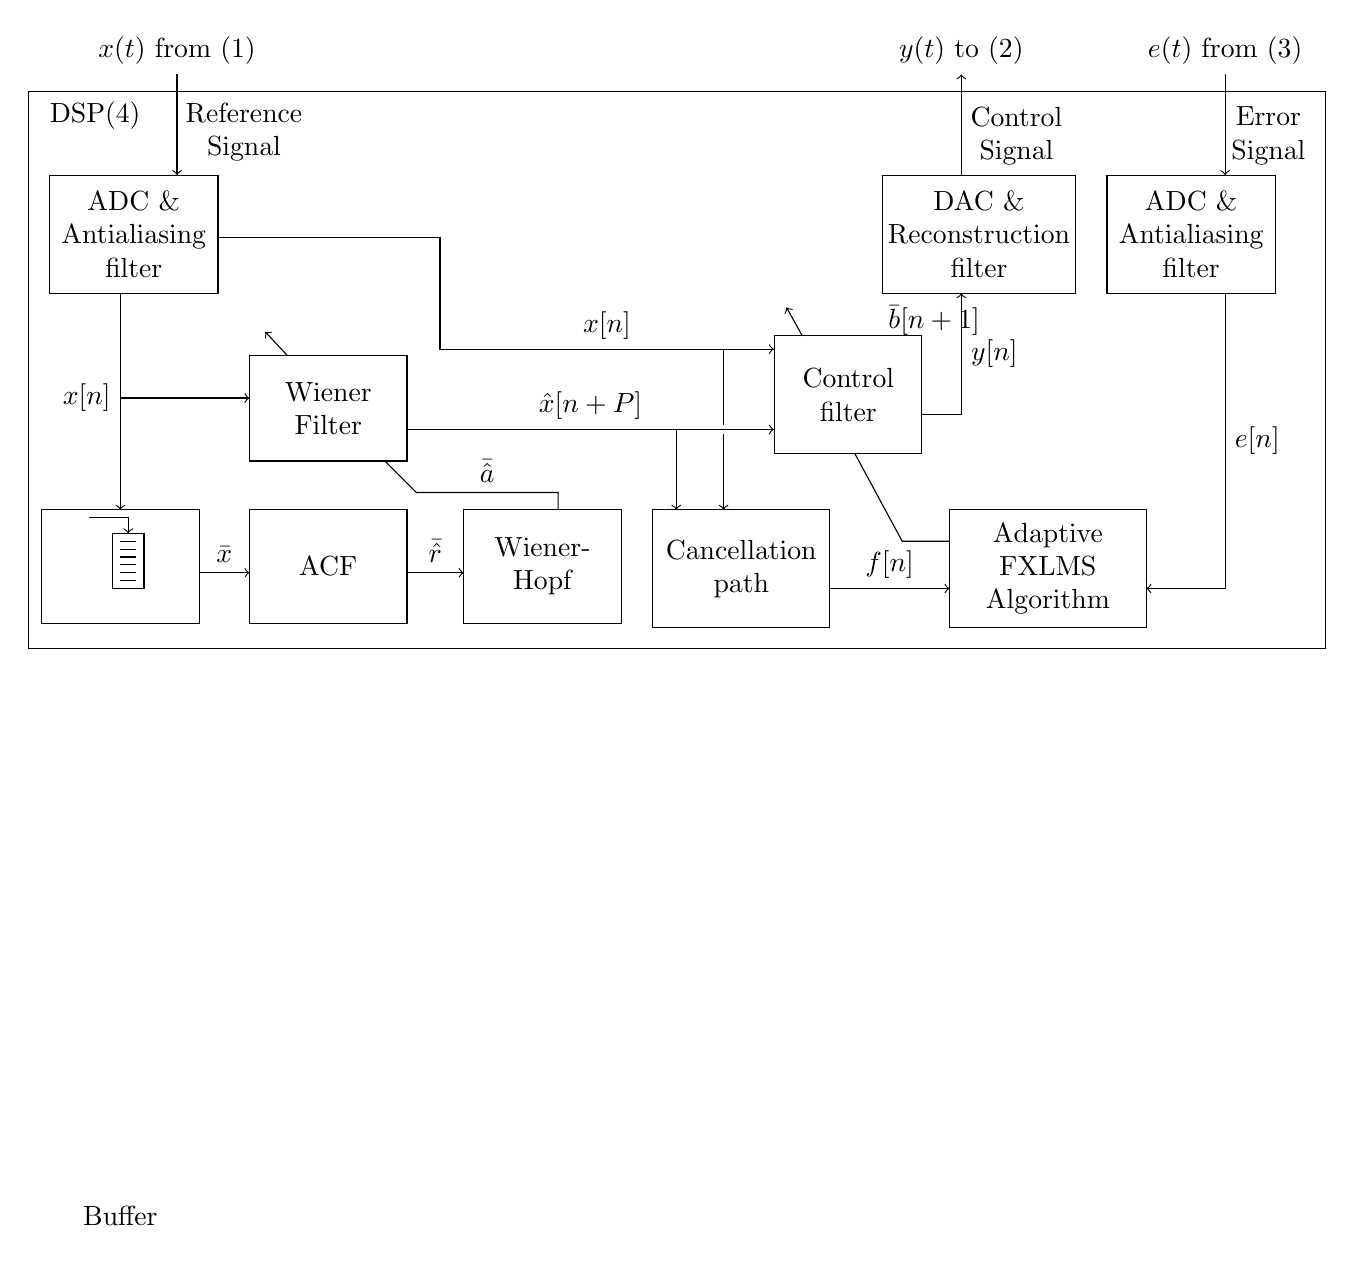
\begin{tikzpicture}
\draw  (-6.96,-2.17) rectangle node[text width=2cm,align=center] {ADC \& Antialiasing filter} (-4.82,-3.67);
\draw  (0.7,-6.42) rectangle node[text width=2.5cm,align=center] {Cancellation \\ path}(2.95,-7.92);
\draw  (4.47,-6.42) rectangle node[text width=2.5cm,align=center] {Adaptive FXLMS Algorithm} (6.97,-7.92);

\draw  (2.25,-4.21) rectangle node[text width=1.5cm,align=center,fill=white] {Control filter} (4.12,-5.71);
\draw  (3.62,-2.17) rectangle node[text width=2.5cm,align=center] {DAC \& \\ Reconstruction filter}(6.07,-3.67);
\draw  (6.47,-2.17) rectangle node[text width=2cm,align=center] {ADC \& Antialiasing filter}(8.61,-3.67);

\draw  (-7.23,-1.11) rectangle (9.25,-8.18);
\node at (-6.38,-1.41) {DSP(4)};
\node [text width=2cm,align=center] at (-4.49,-1.62) {Reference Signal};

\draw[->] (2.95,-7.42) -- node[above]{$f[n]$} (4.47,-7.42);

\draw[->] (7.97,-3.67) -- node[right]{$e[n]$} (7.97,-7.42)  -- (6.97,-7.42);

\draw [->](7.97,-0.89) node[above]{$e(t)$ from (3)} -- (7.97,-2.17) ;
\draw [->](4.62,-2.17)  --  (4.62,-0.89) node[above]{$y(t)$ to (2)};




\draw[->] (4.12,-5.21) -- (4.62,-5.21) --node[right]{$y[n]$} (4.62,-3.67);
\draw [->](-5.34,-0.89) node[above]{$x(t)$ from (1)} -- (-5.34,-2.17);
\node [text width=2cm,align=center] at (5.32,-1.67) {Control Signal};
\node [text width=1.5cm,align=center] at (8.52,-1.67) {Error Signal};

\draw (4.47,-6.82) -- (3.87,-6.82) --node[above=2.25,right]{$\bar{b}[n+1]$} (3.27,-5.71);
\draw [->](2.6,-4.21) -- (2.4,-3.85);


%% Boxes
\draw  (-4.42,-5.8) rectangle node[text width=2cm,align=center] {Wiener Filter}(-2.42,-4.46);
\draw  (-2.42,-6.42) rectangle node[text width=2cm,align=center] {ACF}(-4.42,-7.86);
\draw  (-5.06,-6.42) rectangle node[text width=2cm,align=center,below=8] {Buffer}(-7.06,-7.86);
\draw  (-1.7,-6.42) rectangle node[text width=1.5cm,align=center] {Wiener- Hopf}(0.3,-7.86);



%%Buffer
\draw (-5.76,-7.42) node (v1) {} -- (-6.16,-7.42) -- (-6.16,-6.72) -- (-5.76,-6.72) -- (-5.76,-7.42);
\draw (-6.06,-6.82) -- (-5.86,-6.82);
\draw (-6.06,-6.92) -- (-5.86,-6.92);
\draw (-6.06,-7.02) -- (-5.86,-7.02);
\draw (-6.06,-7.12) -- (-5.86,-7.12);
\draw (-6.06,-7.22) -- (-5.86,-7.22);
\draw (-6.06,-7.32) -- (-5.86,-7.32);
\draw [->](-6.46,-6.52) -- (-5.96,-6.52) -- (-5.96,-6.72);


%% Lines
\draw [->](-5.06,-7.22) -- node[above]{$\bar{x}$} (-4.42,-7.22);
\draw [->](-2.42,-7.22) -- node[above]{$\bar{\hat{r}}$}(-1.7,-7.22);
\draw (-0.5,-6.42) -- (-0.5,-6.2) -- node[above]{$\bar{\hat{a}}$} (-2.3,-6.2) -- (-2.7,-5.8);


\draw [->](-3.94,-4.46) -- (-4.22,-4.16);
\draw [->](-6.06,-5)  node[left]{$x[n]$} -- (-4.42,-5);
\draw [->](-6.06,-3.68) -- (-6.06,-6.42);
\draw [->](-2.42,-5.4) --  node[above]{$\hat{x}[n+P]$}(2.24,-5.4);

\draw [->](-4.82,-2.96) -- (-4.56,-2.96) -- (-2,-2.96) -- (-2,-4.38) -- node[above]{$x[n]$} (2.24,-4.38);
\draw (1.6,-4.38) -- (1.6,-5.34);
\draw [->](1.6,-5.46) -- (1.6,-6.42);
\draw [->](1,-5.4) -- (1,-6.42);
\end{tikzpicture}}
	\end{center}
\end{frame}


\subsection{Multirate}
\begin{frame}{Implementation Consideration}{Multirate}

	\begin{columns}
		\begin{column}{0.4\textwidth}
\begin{itemize}
\item Reduce computation by $2^4$

\begin{itemize}
\item Lower prediction length
\item Effecting 3 kHz slightly at $fs=12 kHz$ 
\end{itemize}
\end{itemize}
		\end{column}
		\begin{column}{0.6\textwidth} 
		
		\begin{center}
\vspace{3mm}
		\resizebox{0.75\columnwidth}{!}{
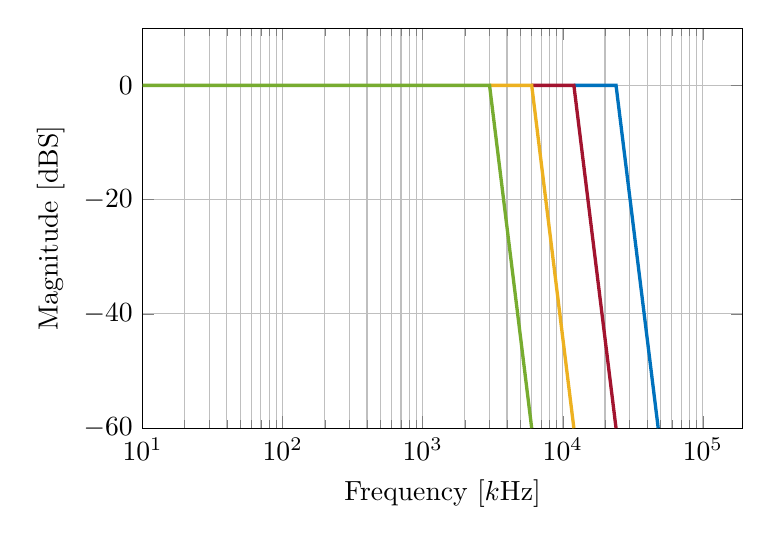
\begin{tikzpicture}
\begin{axis}[
width=3in,
height=2in,
scale only axis,
unbounded coords=jump,
xmode=log,
xmin=10,
xmax=192000,
xminorticks=true,
xlabel={Frequency [$k$Hz]},
xmajorgrids,
xminorgrids,
ymin=-60,
ymax=10,
ylabel={Magnitude [dBS]},
ymajorgrids,
axis background/.style={fill=white},
]
\addplot[mark=none, MATLABblue,very thick] coordinates {(12000,0) (24000,0) (48000,-60)};
\addplot[mark=none, MATLABred,very thick] coordinates {(6000,0) (12000,0) (24000,-60)};
\addplot[mark=none, MATLAByellow,very thick] coordinates {(3000,0) (6000,0) (12000,-60)};
\addplot[mark=none, MATLABgreen,very thick] coordinates {(10,0) (3000,0) (6000,-60)};
\end{axis}
\end{tikzpicture}
}
		\end{center}	
		\end{column}
	\end{columns}
\begin{table}[]
	\centering
	\begin{tabular}{|c|c|c|c|c|c|}
		\hline
		$fs$                                                          & 192 & \textcolor{MATLABblue}{96} & \textcolor{MATLABred}{48} & \textcolor{MATLAByellow}{24} & \textcolor{MATLABgreen}{12} \\ \hline
		Time                                                          & 225 $\mu s$ & \textcolor{MATLABblue}{225 $\mu s$ } & \textcolor{MATLABred}{225 $\mu s$ } & \textcolor{MATLAByellow}{225 $\mu s$ } & \textcolor{MATLABgreen}{225 $\mu s$ } \\ \hline
		\begin{tabular}[c]{@{}c@{}}Prediction\\ Length\end{tabular}   & 43  &\textcolor{MATLABblue}{22} & \textcolor{MATLABred}{11} & \textcolor{MATLAByellow}{6}  & \textcolor{MATLABgreen}{3}  \\ \hline
	\end{tabular}
\end{table}	
\end{frame}

%\section{Combined system}
\begin{frame}{Methods}{Combined System}	
		\begin{itemize}
			\item Input for control filter and CP
			\begin{itemize}
			\item $x[n]$
			\item $\hat{x}[n+P]$
			\end{itemize}
		\end{itemize}
\begin{center}
	\resizebox{0.9\columnwidth}{!}{		
			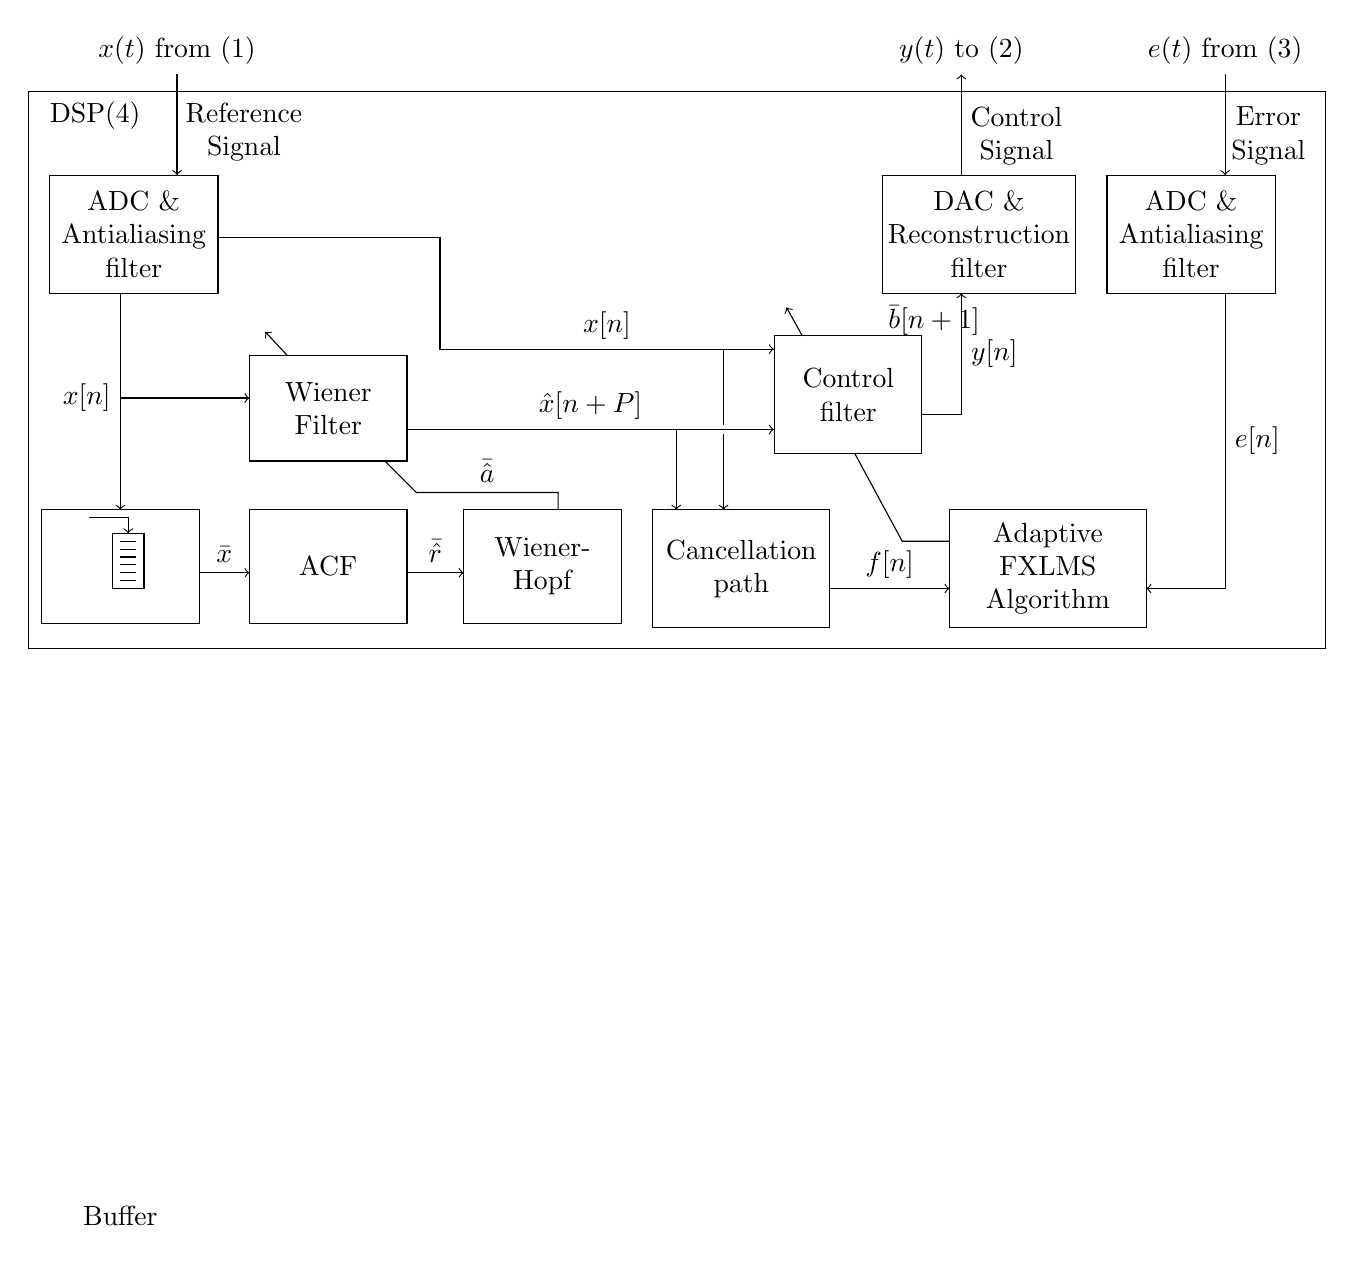
\begin{tikzpicture}
\draw  (-6.96,-2.17) rectangle node[text width=2cm,align=center] {ADC \& Antialiasing filter} (-4.82,-3.67);
\draw  (0.7,-6.42) rectangle node[text width=2.5cm,align=center] {Cancellation \\ path}(2.95,-7.92);
\draw  (4.47,-6.42) rectangle node[text width=2.5cm,align=center] {Adaptive FXLMS Algorithm} (6.97,-7.92);

\draw  (2.25,-4.21) rectangle node[text width=1.5cm,align=center,fill=white] {Control filter} (4.12,-5.71);
\draw  (3.62,-2.17) rectangle node[text width=2.5cm,align=center] {DAC \& \\ Reconstruction filter}(6.07,-3.67);
\draw  (6.47,-2.17) rectangle node[text width=2cm,align=center] {ADC \& Antialiasing filter}(8.61,-3.67);

\draw  (-7.23,-1.11) rectangle (9.25,-8.18);
\node at (-6.38,-1.41) {DSP(4)};
\node [text width=2cm,align=center] at (-4.49,-1.62) {Reference Signal};

\draw[->] (2.95,-7.42) -- node[above]{$f[n]$} (4.47,-7.42);

\draw[->] (7.97,-3.67) -- node[right]{$e[n]$} (7.97,-7.42)  -- (6.97,-7.42);

\draw [->](7.97,-0.89) node[above]{$e(t)$ from (3)} -- (7.97,-2.17) ;
\draw [->](4.62,-2.17)  --  (4.62,-0.89) node[above]{$y(t)$ to (2)};




\draw[->] (4.12,-5.21) -- (4.62,-5.21) --node[right]{$y[n]$} (4.62,-3.67);
\draw [->](-5.34,-0.89) node[above]{$x(t)$ from (1)} -- (-5.34,-2.17);
\node [text width=2cm,align=center] at (5.32,-1.67) {Control Signal};
\node [text width=1.5cm,align=center] at (8.52,-1.67) {Error Signal};

\draw (4.47,-6.82) -- (3.87,-6.82) --node[above=2.25,right]{$\bar{b}[n+1]$} (3.27,-5.71);
\draw [->](2.6,-4.21) -- (2.4,-3.85);


%% Boxes
\draw  (-4.42,-5.8) rectangle node[text width=2cm,align=center] {Wiener Filter}(-2.42,-4.46);
\draw  (-2.42,-6.42) rectangle node[text width=2cm,align=center] {ACF}(-4.42,-7.86);
\draw  (-5.06,-6.42) rectangle node[text width=2cm,align=center,below=8] {Buffer}(-7.06,-7.86);
\draw  (-1.7,-6.42) rectangle node[text width=1.5cm,align=center] {Wiener- Hopf}(0.3,-7.86);



%%Buffer
\draw (-5.76,-7.42) node (v1) {} -- (-6.16,-7.42) -- (-6.16,-6.72) -- (-5.76,-6.72) -- (-5.76,-7.42);
\draw (-6.06,-6.82) -- (-5.86,-6.82);
\draw (-6.06,-6.92) -- (-5.86,-6.92);
\draw (-6.06,-7.02) -- (-5.86,-7.02);
\draw (-6.06,-7.12) -- (-5.86,-7.12);
\draw (-6.06,-7.22) -- (-5.86,-7.22);
\draw (-6.06,-7.32) -- (-5.86,-7.32);
\draw [->](-6.46,-6.52) -- (-5.96,-6.52) -- (-5.96,-6.72);


%% Lines
\draw [->](-5.06,-7.22) -- node[above]{$\bar{x}$} (-4.42,-7.22);
\draw [->](-2.42,-7.22) -- node[above]{$\bar{\hat{r}}$}(-1.7,-7.22);
\draw (-0.5,-6.42) -- (-0.5,-6.2) -- node[above]{$\bar{\hat{a}}$} (-2.3,-6.2) -- (-2.7,-5.8);


\draw [->](-3.94,-4.46) -- (-4.22,-4.16);
\draw [->](-6.06,-5)  node[left]{$x[n]$} -- (-4.42,-5);
\draw [->](-6.06,-3.68) -- (-6.06,-6.42);
\draw [->](-2.42,-5.4) --  node[above]{$\hat{x}[n+P]$}(2.24,-5.4);

\draw [->](-4.82,-2.96) -- (-4.56,-2.96) -- (-2,-2.96) -- (-2,-4.38) -- node[above]{$x[n]$} (2.24,-4.38);
\draw (1.6,-4.38) -- (1.6,-5.34);
\draw [->](1.6,-5.46) -- (1.6,-6.42);
\draw [->](1,-5.4) -- (1,-6.42);
\end{tikzpicture}}
\end{center}
\end{frame}



\section{Simulations}
\subsection{How to test}

\begin{frame}{Simulation}{What to test?}	
\begin{itemize}
	\item Linear Prediction
	\begin{itemize}
		\item Optimal parameters for LP ($N$,$O$,$f_s$,$P$)
	\end{itemize}
	\item Feedforward FXLMS	
	\begin{itemize}
		\item Attenuation with different delays
		\item Frequency response
	\end{itemize}
\end{itemize}
\end{frame}

\begin{frame}{Simulation}{How to Test}	
\begin{itemize}
	\item Simulink
	\item Simulating with two systems 
	\begin{itemize}
		\item Linear Prediction
		\item Feedforward FXLMS
		\item Sound files are adapted 
	\end{itemize}
	\item Automation of simulations	
\end{itemize}
\end{frame}

\begin{frame}{Simulation}{How to Test}	
\begin{itemize}
	\item Archimedes Project		
\end{itemize}
\end{frame}


\begin{frame}{Simulation Results}{Analysis of results}	
\begin{itemize}
	\item Linear Prediction
	\begin{itemize}
		\item Prediction Gain: $PG = 10 log_{10}\bigg(\frac{\sigma^2_x}{\sigma^2_\varepsilon}\bigg) = 10 log_{10}\bigg(\frac{E\{x^2[n]\}}{E\{\varepsilon^2[n]\}}\bigg)$
	\end{itemize}
	\item Feedforward FXLMS
	\begin{itemize}
		\item Filter-bank
	\end{itemize}
\end{itemize}
\end{frame}


\subsection{Linear Prediction Parameters}
\begin{frame}{Simulation Results}{Optimal parameters}		
\begin{columns}
	\begin{column}{0.4\textwidth}
		\begin{itemize}
			\item Prediction order P = 43
			\item Optimal parameters
			\begin{itemize}
				\item Framelength N = 1600
				\item Overlap O = 1500
			\end{itemize}
			\item Prediction Gain PG = 5.4 dB
		\end{itemize}
	\end{column}
	\begin{column}{0.6\textwidth} 
		\resizebox{0.9\columnwidth}{!}{		
			% This file was created by matlab2tikz.
%
%The latest updates can be retrieved from
%  http://www.mathworks.com/matlabcentral/fileexchange/22022-matlab2tikz-matlab2tikz
%where you can also make suggestions and rate matlab2tikz.
%
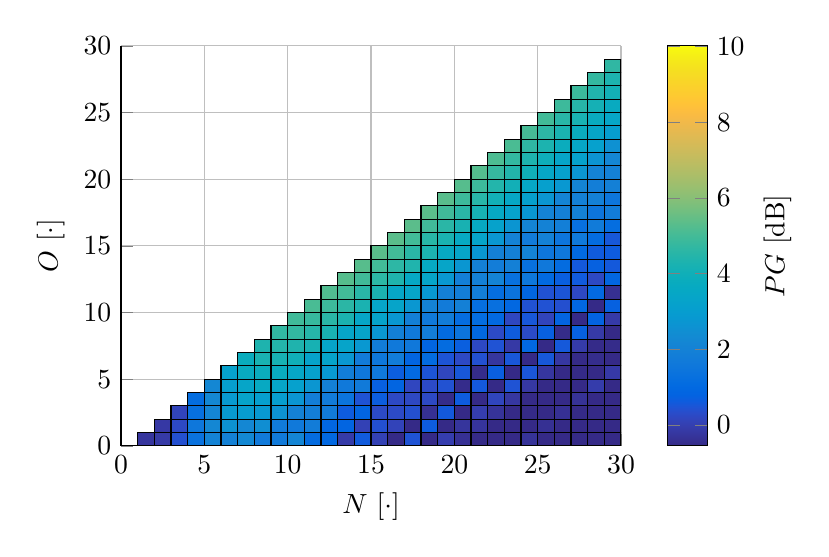
\begin{tikzpicture}


\begin{axis}[%
width=2.5in,
height=2in,
scale only axis,
point meta min=-0.551769511455843,
point meta max=10.0207598959184,
unbounded coords=jump,
xmin=0,
xmax=3000,
xlabel={$N$ [$\cdot$]},
xmajorgrids,
ymin=0,
ymax=3000,
ytick={0,500,...,3000},
yticklabels={0,5,...,30},
xtick={0,500,...,3000},
xticklabels={0,5,...,30},
ylabel={$O$ [$\cdot$]},
ymajorgrids,
axis background/.style={fill=white},
axis x line*=bottom,
axis y line*=left,
colormap={mymap}{[1pt] rgb(0pt)=(0.2081,0.1663,0.5292); rgb(1pt)=(0.211624,0.189781,0.577676); rgb(2pt)=(0.212252,0.213771,0.626971); rgb(3pt)=(0.2081,0.2386,0.677086); rgb(4pt)=(0.195905,0.264457,0.7279); rgb(5pt)=(0.170729,0.291938,0.779248); rgb(6pt)=(0.125271,0.324243,0.830271); rgb(7pt)=(0.0591333,0.359833,0.868333); rgb(8pt)=(0.0116952,0.38751,0.881957); rgb(9pt)=(0.00595714,0.408614,0.882843); rgb(10pt)=(0.0165143,0.4266,0.878633); rgb(11pt)=(0.0328524,0.443043,0.871957); rgb(12pt)=(0.0498143,0.458571,0.864057); rgb(13pt)=(0.0629333,0.47369,0.855438); rgb(14pt)=(0.0722667,0.488667,0.8467); rgb(15pt)=(0.0779429,0.503986,0.838371); rgb(16pt)=(0.0793476,0.520024,0.831181); rgb(17pt)=(0.0749429,0.537543,0.826271); rgb(18pt)=(0.0640571,0.556986,0.823957); rgb(19pt)=(0.0487714,0.577224,0.822829); rgb(20pt)=(0.0343429,0.596581,0.819852); rgb(21pt)=(0.0265,0.6137,0.8135); rgb(22pt)=(0.0238905,0.628662,0.803762); rgb(23pt)=(0.0230905,0.641786,0.791267); rgb(24pt)=(0.0227714,0.653486,0.776757); rgb(25pt)=(0.0266619,0.664195,0.760719); rgb(26pt)=(0.0383714,0.674271,0.743552); rgb(27pt)=(0.0589714,0.683757,0.725386); rgb(28pt)=(0.0843,0.692833,0.706167); rgb(29pt)=(0.113295,0.7015,0.685857); rgb(30pt)=(0.145271,0.709757,0.664629); rgb(31pt)=(0.180133,0.717657,0.642433); rgb(32pt)=(0.217829,0.725043,0.619262); rgb(33pt)=(0.258643,0.731714,0.595429); rgb(34pt)=(0.302171,0.737605,0.571186); rgb(35pt)=(0.348167,0.742433,0.547267); rgb(36pt)=(0.395257,0.7459,0.524443); rgb(37pt)=(0.44201,0.748081,0.503314); rgb(38pt)=(0.487124,0.749062,0.483976); rgb(39pt)=(0.530029,0.749114,0.466114); rgb(40pt)=(0.570857,0.748519,0.44939); rgb(41pt)=(0.609852,0.747314,0.433686); rgb(42pt)=(0.6473,0.7456,0.4188); rgb(43pt)=(0.683419,0.743476,0.404433); rgb(44pt)=(0.71841,0.741133,0.390476); rgb(45pt)=(0.752486,0.7384,0.376814); rgb(46pt)=(0.785843,0.735567,0.363271); rgb(47pt)=(0.818505,0.732733,0.34979); rgb(48pt)=(0.850657,0.7299,0.336029); rgb(49pt)=(0.882433,0.727433,0.3217); rgb(50pt)=(0.913933,0.725786,0.306276); rgb(51pt)=(0.944957,0.726114,0.288643); rgb(52pt)=(0.973895,0.731395,0.266648); rgb(53pt)=(0.993771,0.745457,0.240348); rgb(54pt)=(0.999043,0.765314,0.216414); rgb(55pt)=(0.995533,0.786057,0.196652); rgb(56pt)=(0.988,0.8066,0.179367); rgb(57pt)=(0.978857,0.827143,0.163314); rgb(58pt)=(0.9697,0.848138,0.147452); rgb(59pt)=(0.962586,0.870514,0.1309); rgb(60pt)=(0.958871,0.8949,0.113243); rgb(61pt)=(0.959824,0.921833,0.0948381); rgb(62pt)=(0.9661,0.951443,0.0755333); rgb(63pt)=(0.9763,0.9831,0.0538)},
colorbar,
colorbar style={ylabel={$PG$ [dB]}}
]

\addplot[%
surf,
shader=flat corner,draw=black,colormap={mymap}{[1pt] rgb(0pt)=(0.2081,0.1663,0.5292); rgb(1pt)=(0.211624,0.189781,0.577676); rgb(2pt)=(0.212252,0.213771,0.626971); rgb(3pt)=(0.2081,0.2386,0.677086); rgb(4pt)=(0.195905,0.264457,0.7279); rgb(5pt)=(0.170729,0.291938,0.779248); rgb(6pt)=(0.125271,0.324243,0.830271); rgb(7pt)=(0.0591333,0.359833,0.868333); rgb(8pt)=(0.0116952,0.38751,0.881957); rgb(9pt)=(0.00595714,0.408614,0.882843); rgb(10pt)=(0.0165143,0.4266,0.878633); rgb(11pt)=(0.0328524,0.443043,0.871957); rgb(12pt)=(0.0498143,0.458571,0.864057); rgb(13pt)=(0.0629333,0.47369,0.855438); rgb(14pt)=(0.0722667,0.488667,0.8467); rgb(15pt)=(0.0779429,0.503986,0.838371); rgb(16pt)=(0.0793476,0.520024,0.831181); rgb(17pt)=(0.0749429,0.537543,0.826271); rgb(18pt)=(0.0640571,0.556986,0.823957); rgb(19pt)=(0.0487714,0.577224,0.822829); rgb(20pt)=(0.0343429,0.596581,0.819852); rgb(21pt)=(0.0265,0.6137,0.8135); rgb(22pt)=(0.0238905,0.628662,0.803762); rgb(23pt)=(0.0230905,0.641786,0.791267); rgb(24pt)=(0.0227714,0.653486,0.776757); rgb(25pt)=(0.0266619,0.664195,0.760719); rgb(26pt)=(0.0383714,0.674271,0.743552); rgb(27pt)=(0.0589714,0.683757,0.725386); rgb(28pt)=(0.0843,0.692833,0.706167); rgb(29pt)=(0.113295,0.7015,0.685857); rgb(30pt)=(0.145271,0.709757,0.664629); rgb(31pt)=(0.180133,0.717657,0.642433); rgb(32pt)=(0.217829,0.725043,0.619262); rgb(33pt)=(0.258643,0.731714,0.595429); rgb(34pt)=(0.302171,0.737605,0.571186); rgb(35pt)=(0.348167,0.742433,0.547267); rgb(36pt)=(0.395257,0.7459,0.524443); rgb(37pt)=(0.44201,0.748081,0.503314); rgb(38pt)=(0.487124,0.749062,0.483976); rgb(39pt)=(0.530029,0.749114,0.466114); rgb(40pt)=(0.570857,0.748519,0.44939); rgb(41pt)=(0.609852,0.747314,0.433686); rgb(42pt)=(0.6473,0.7456,0.4188); rgb(43pt)=(0.683419,0.743476,0.404433); rgb(44pt)=(0.71841,0.741133,0.390476); rgb(45pt)=(0.752486,0.7384,0.376814); rgb(46pt)=(0.785843,0.735567,0.363271); rgb(47pt)=(0.818505,0.732733,0.34979); rgb(48pt)=(0.850657,0.7299,0.336029); rgb(49pt)=(0.882433,0.727433,0.3217); rgb(50pt)=(0.913933,0.725786,0.306276); rgb(51pt)=(0.944957,0.726114,0.288643); rgb(52pt)=(0.973895,0.731395,0.266648); rgb(53pt)=(0.993771,0.745457,0.240348); rgb(54pt)=(0.999043,0.765314,0.216414); rgb(55pt)=(0.995533,0.786057,0.196652); rgb(56pt)=(0.988,0.8066,0.179367); rgb(57pt)=(0.978857,0.827143,0.163314); rgb(58pt)=(0.9697,0.848138,0.147452); rgb(59pt)=(0.962586,0.870514,0.1309); rgb(60pt)=(0.958871,0.8949,0.113243); rgb(61pt)=(0.959824,0.921833,0.0948381); rgb(62pt)=(0.9661,0.951443,0.0755333); rgb(63pt)=(0.9763,0.9831,0.0538)},mesh/rows=30]
table[row sep=crcr, point meta=\thisrow{c}] {%
	%
	x	y	c\\
	100	0	-0.249851110691807\\
	100	100	nan\\
	100	200	nan\\
	100	300	nan\\
	100	400	nan\\
	100	500	nan\\
	100	600	nan\\
	100	700	nan\\
	100	800	nan\\
	100	900	nan\\
	100	1000	nan\\
	100	1100	nan\\
	100	1200	nan\\
	100	1300	nan\\
	100	1400	nan\\
	100	1500	nan\\
	100	1600	nan\\
	100	1700	nan\\
	100	1800	nan\\
	100	1900	nan\\
	100	2000	nan\\
	100	2100	nan\\
	100	2200	nan\\
	100	2300	nan\\
	100	2400	nan\\
	100	2500	nan\\
	100	2600	nan\\
	100	2700	nan\\
	100	2800	nan\\
	100	2900	nan\\
	200	0	-0.134212977797894\\
	200	100	-0.167103642187056\\
	200	200	nan\\
	200	300	nan\\
	200	400	nan\\
	200	500	nan\\
	200	600	nan\\
	200	700	nan\\
	200	800	nan\\
	200	900	nan\\
	200	1000	nan\\
	200	1100	nan\\
	200	1200	nan\\
	200	1300	nan\\
	200	1400	nan\\
	200	1500	nan\\
	200	1600	nan\\
	200	1700	nan\\
	200	1800	nan\\
	200	1900	nan\\
	200	2000	nan\\
	200	2100	nan\\
	200	2200	nan\\
	200	2300	nan\\
	200	2400	nan\\
	200	2500	nan\\
	200	2600	nan\\
	200	2700	nan\\
	200	2800	nan\\
	200	2900	nan\\
	300	0	0.40073258158409\\
	300	100	0.251927782024709\\
	300	200	0.142801564300892\\
	300	300	nan\\
	300	400	nan\\
	300	500	nan\\
	300	600	nan\\
	300	700	nan\\
	300	800	nan\\
	300	900	nan\\
	300	1000	nan\\
	300	1100	nan\\
	300	1200	nan\\
	300	1300	nan\\
	300	1400	nan\\
	300	1500	nan\\
	300	1600	nan\\
	300	1700	nan\\
	300	1800	nan\\
	300	1900	nan\\
	300	2000	nan\\
	300	2100	nan\\
	300	2200	nan\\
	300	2300	nan\\
	300	2400	nan\\
	300	2500	nan\\
	300	2600	nan\\
	300	2700	nan\\
	300	2800	nan\\
	300	2900	nan\\
	400	0	1.35498518276026\\
	400	100	1.54062929586375\\
	400	200	1.25091430573651\\
	400	300	1.13011541776478\\
	400	400	nan\\
	400	500	nan\\
	400	600	nan\\
	400	700	nan\\
	400	800	nan\\
	400	900	nan\\
	400	1000	nan\\
	400	1100	nan\\
	400	1200	nan\\
	400	1300	nan\\
	400	1400	nan\\
	400	1500	nan\\
	400	1600	nan\\
	400	1700	nan\\
	400	1800	nan\\
	400	1900	nan\\
	400	2000	nan\\
	400	2100	nan\\
	400	2200	nan\\
	400	2300	nan\\
	400	2400	nan\\
	400	2500	nan\\
	400	2600	nan\\
	400	2700	nan\\
	400	2800	nan\\
	400	2900	nan\\
	500	0	2.07613030072784\\
	500	100	2.23484268450241\\
	500	200	2.16667780407076\\
	500	300	2.22280459708376\\
	500	400	2.22773910206715\\
	500	500	nan\\
	500	600	nan\\
	500	700	nan\\
	500	800	nan\\
	500	900	nan\\
	500	1000	nan\\
	500	1100	nan\\
	500	1200	nan\\
	500	1300	nan\\
	500	1400	nan\\
	500	1500	nan\\
	500	1600	nan\\
	500	1700	nan\\
	500	1800	nan\\
	500	1900	nan\\
	500	2000	nan\\
	500	2100	nan\\
	500	2200	nan\\
	500	2300	nan\\
	500	2400	nan\\
	500	2500	nan\\
	500	2600	nan\\
	500	2700	nan\\
	500	2800	nan\\
	500	2900	nan\\
	600	0	2.0053564589082\\
	600	100	2.61259722918176\\
	600	200	2.8832092344045\\
	600	300	2.86284941749047\\
	600	400	3.10314445957564\\
	600	500	3.19779941497919\\
	600	600	nan\\
	600	700	nan\\
	600	800	nan\\
	600	900	nan\\
	600	1000	nan\\
	600	1100	nan\\
	600	1200	nan\\
	600	1300	nan\\
	600	1400	nan\\
	600	1500	nan\\
	600	1600	nan\\
	600	1700	nan\\
	600	1800	nan\\
	600	1900	nan\\
	600	2000	nan\\
	600	2100	nan\\
	600	2200	nan\\
	600	2300	nan\\
	600	2400	nan\\
	600	2500	nan\\
	600	2600	nan\\
	600	2700	nan\\
	600	2800	nan\\
	600	2900	nan\\
	700	0	2.2744146608244\\
	700	100	2.21229720700257\\
	700	200	2.93838458205897\\
	700	300	3.29709652218325\\
	700	400	3.37210041995159\\
	700	500	3.73517577501174\\
	700	600	3.8204270648783\\
	700	700	nan\\
	700	800	nan\\
	700	900	nan\\
	700	1000	nan\\
	700	1100	nan\\
	700	1200	nan\\
	700	1300	nan\\
	700	1400	nan\\
	700	1500	nan\\
	700	1600	nan\\
	700	1700	nan\\
	700	1800	nan\\
	700	1900	nan\\
	700	2000	nan\\
	700	2100	nan\\
	700	2200	nan\\
	700	2300	nan\\
	700	2400	nan\\
	700	2500	nan\\
	700	2600	nan\\
	700	2700	nan\\
	700	2800	nan\\
	700	2900	nan\\
	800	0	1.6764398517674\\
	800	100	2.47790908751089\\
	800	200	2.84811066063823\\
	800	300	3.0687707331656\\
	800	400	3.63876502838183\\
	800	500	3.84993979572264\\
	800	600	4.22707612972411\\
	800	700	4.34417470624987\\
	800	800	nan\\
	800	900	nan\\
	800	1000	nan\\
	800	1100	nan\\
	800	1200	nan\\
	800	1300	nan\\
	800	1400	nan\\
	800	1500	nan\\
	800	1600	nan\\
	800	1700	nan\\
	800	1800	nan\\
	800	1900	nan\\
	800	2000	nan\\
	800	2100	nan\\
	800	2200	nan\\
	800	2300	nan\\
	800	2400	nan\\
	800	2500	nan\\
	800	2600	nan\\
	800	2700	nan\\
	800	2800	nan\\
	800	2900	nan\\
	900	0	1.6957478568352\\
	900	100	1.7319915851467\\
	900	200	2.60512775573002\\
	900	300	2.98481824622671\\
	900	400	3.37091511369957\\
	900	500	3.74946849304965\\
	900	600	4.17472244368776\\
	900	700	4.46545647083027\\
	900	800	4.70107297446204\\
	900	900	nan\\
	900	1000	nan\\
	900	1100	nan\\
	900	1200	nan\\
	900	1300	nan\\
	900	1400	nan\\
	900	1500	nan\\
	900	1600	nan\\
	900	1700	nan\\
	900	1800	nan\\
	900	1900	nan\\
	900	2000	nan\\
	900	2100	nan\\
	900	2200	nan\\
	900	2300	nan\\
	900	2400	nan\\
	900	2500	nan\\
	900	2600	nan\\
	900	2700	nan\\
	900	2800	nan\\
	900	2900	nan\\
	1000	0	2.14279356476327\\
	1000	100	1.65662756562456\\
	1000	200	1.9975093051342\\
	1000	300	2.68811548919998\\
	1000	400	3.15564116436878\\
	1000	500	3.43923191192347\\
	1000	600	4.00698906883707\\
	1000	700	4.36135318968568\\
	1000	800	4.71880877909074\\
	1000	900	4.9493889064919\\
	1000	1000	nan\\
	1000	1100	nan\\
	1000	1200	nan\\
	1000	1300	nan\\
	1000	1400	nan\\
	1000	1500	nan\\
	1000	1600	nan\\
	1000	1700	nan\\
	1000	1800	nan\\
	1000	1900	nan\\
	1000	2000	nan\\
	1000	2100	nan\\
	1000	2200	nan\\
	1000	2300	nan\\
	1000	2400	nan\\
	1000	2500	nan\\
	1000	2600	nan\\
	1000	2700	nan\\
	1000	2800	nan\\
	1000	2900	nan\\
	1100	0	1.08628380389681\\
	1100	100	1.78373115008797\\
	1100	200	1.83869495569938\\
	1100	300	1.84921642836682\\
	1100	400	2.72090762354963\\
	1100	500	3.19932951902192\\
	1100	600	3.28763346728818\\
	1100	700	4.1733005127402\\
	1100	800	4.49383265009054\\
	1100	900	4.81677388898654\\
	1100	1000	5.09223132392375\\
	1100	1100	nan\\
	1100	1200	nan\\
	1100	1300	nan\\
	1100	1400	nan\\
	1100	1500	nan\\
	1100	1600	nan\\
	1100	1700	nan\\
	1100	1800	nan\\
	1100	1900	nan\\
	1100	2000	nan\\
	1100	2100	nan\\
	1100	2200	nan\\
	1100	2300	nan\\
	1100	2400	nan\\
	1100	2500	nan\\
	1100	2600	nan\\
	1100	2700	nan\\
	1100	2800	nan\\
	1100	2900	nan\\
	1200	0	0.96228292179036\\
	1200	100	0.874714526881095\\
	1200	200	1.74822965859813\\
	1200	300	1.74613873946482\\
	1200	400	1.96406088862939\\
	1200	500	2.83528036765025\\
	1200	600	3.27582233051984\\
	1200	700	3.34225172739605\\
	1200	800	4.2270814155954\\
	1200	900	4.5852271687131\\
	1200	1000	4.90782372375419\\
	1200	1100	5.19666553372495\\
	1200	1200	nan\\
	1200	1300	nan\\
	1200	1400	nan\\
	1200	1500	nan\\
	1200	1600	nan\\
	1200	1700	nan\\
	1200	1800	nan\\
	1200	1900	nan\\
	1200	2000	nan\\
	1200	2100	nan\\
	1200	2200	nan\\
	1200	2300	nan\\
	1200	2400	nan\\
	1200	2500	nan\\
	1200	2600	nan\\
	1200	2700	nan\\
	1200	2800	nan\\
	1200	2900	nan\\
	1300	0	-0.107030717223719\\
	1300	100	0.850232560605215\\
	1300	200	0.637949811893221\\
	1300	300	1.40384792467279\\
	1300	400	1.64958254277473\\
	1300	500	1.79741249348277\\
	1300	600	2.75608764238935\\
	1300	700	3.32534859240284\\
	1300	800	3.40167471419125\\
	1300	900	4.26932143570372\\
	1300	1000	4.60365364811444\\
	1300	1100	4.98195949948451\\
	1300	1200	5.28042149364273\\
	1300	1300	nan\\
	1300	1400	nan\\
	1300	1500	nan\\
	1300	1600	nan\\
	1300	1700	nan\\
	1300	1800	nan\\
	1300	1900	nan\\
	1300	2000	nan\\
	1300	2100	nan\\
	1300	2200	nan\\
	1300	2300	nan\\
	1300	2400	nan\\
	1300	2500	nan\\
	1300	2600	nan\\
	1300	2700	nan\\
	1300	2800	nan\\
	1300	2900	nan\\
	1400	0	0.601907313869925\\
	1400	100	0.0657729838043244\\
	1400	200	0.862145199127073\\
	1400	300	0.460707580490794\\
	1400	400	1.68525830954437\\
	1400	500	1.55802793388997\\
	1400	600	1.74594940231651\\
	1400	700	2.81551743753557\\
	1400	800	3.32371598632194\\
	1400	900	3.42520085860678\\
	1400	1000	4.25956377468848\\
	1400	1100	4.56477323219294\\
	1400	1200	4.97384046578701\\
	1400	1300	5.29633096641679\\
	1400	1400	nan\\
	1400	1500	nan\\
	1400	1600	nan\\
	1400	1700	nan\\
	1400	1800	nan\\
	1400	1900	nan\\
	1400	2000	nan\\
	1400	2100	nan\\
	1400	2200	nan\\
	1400	2300	nan\\
	1400	2400	nan\\
	1400	2500	nan\\
	1400	2600	nan\\
	1400	2700	nan\\
	1400	2800	nan\\
	1400	2900	nan\\
	1500	0	0.0479688920623348\\
	1500	100	0.409815317960011\\
	1500	200	0.265969244574455\\
	1500	300	0.66329040490881\\
	1500	400	0.725248934820509\\
	1500	500	1.62075499462296\\
	1500	600	1.53068266641447\\
	1500	700	1.78380983455356\\
	1500	800	2.75223306087479\\
	1500	900	3.29361894997763\\
	1500	1000	3.36423431504327\\
	1500	1100	4.28085176540069\\
	1500	1200	4.61221553749839\\
	1500	1300	4.99326970538795\\
	1500	1400	5.32976716671813\\
	1500	1500	nan\\
	1500	1600	nan\\
	1500	1700	nan\\
	1500	1800	nan\\
	1500	1900	nan\\
	1500	2000	nan\\
	1500	2100	nan\\
	1500	2200	nan\\
	1500	2300	nan\\
	1500	2400	nan\\
	1500	2500	nan\\
	1500	2600	nan\\
	1500	2700	nan\\
	1500	2800	nan\\
	1500	2900	nan\\
	1600	0	-0.605169389430681\\
	1600	100	0.117420548822926\\
	1600	200	0.284797641762555\\
	1600	300	0.253253520189372\\
	1600	400	0.870129979674615\\
	1600	500	0.671127168444688\\
	1600	600	1.74986538278574\\
	1600	700	1.64439306142093\\
	1600	800	1.91148110154675\\
	1600	900	2.77573952375898\\
	1600	1000	3.32540102344824\\
	1600	1100	3.44971766694812\\
	1600	1200	4.36003073667673\\
	1600	1300	4.62738934446695\\
	1600	1400	4.98723836519226\\
	1600	1500	5.34050250023747\\
	1600	1600	nan\\
	1600	1700	nan\\
	1600	1800	nan\\
	1600	1900	nan\\
	1600	2000	nan\\
	1600	2100	nan\\
	1600	2200	nan\\
	1600	2300	nan\\
	1600	2400	nan\\
	1600	2500	nan\\
	1600	2600	nan\\
	1600	2700	nan\\
	1600	2800	nan\\
	1600	2900	nan\\
	1700	0	0.459481577183121\\
	1700	100	-0.828238464808588\\
	1700	200	0.392172946743951\\
	1700	300	0.226384351456075\\
	1700	400	0.183454984733797\\
	1700	500	1.03300677343369\\
	1700	600	0.866722268193889\\
	1700	700	1.60939528933199\\
	1700	800	1.64458351852261\\
	1700	900	1.91984952325872\\
	1700	1000	2.75640854387435\\
	1700	1100	3.37358423554233\\
	1700	1200	3.57831957034059\\
	1700	1300	4.38037462195002\\
	1700	1400	4.57895857617312\\
	1700	1500	4.99333526811925\\
	1700	1600	5.35096269740123\\
	1700	1700	nan\\
	1700	1800	nan\\
	1700	1900	nan\\
	1700	2000	nan\\
	1700	2100	nan\\
	1700	2200	nan\\
	1700	2300	nan\\
	1700	2400	nan\\
	1700	2500	nan\\
	1700	2600	nan\\
	1700	2700	nan\\
	1700	2800	nan\\
	1700	2900	nan\\
	1800	0	-1.41853543923144\\
	1800	100	0.632649966343857\\
	1800	200	-0.384497042533314\\
	1800	300	0.255556860908392\\
	1800	400	0.286777052802089\\
	1800	500	0.482107568083193\\
	1800	600	1.07739734854062\\
	1800	700	0.851941681167397\\
	1800	800	1.82437185471004\\
	1800	900	1.65998697525295\\
	1800	1000	2.01342546713771\\
	1800	1100	2.84347279090459\\
	1800	1200	3.39849928401779\\
	1800	1300	3.59204978113913\\
	1800	1400	4.2917812700128\\
	1800	1500	4.54262260148609\\
	1800	1600	4.9656993136051\\
	1800	1700	5.33339229740171\\
	1800	1800	nan\\
	1800	1900	nan\\
	1800	2000	nan\\
	1800	2100	nan\\
	1800	2200	nan\\
	1800	2300	nan\\
	1800	2400	nan\\
	1800	2500	nan\\
	1800	2600	nan\\
	1800	2700	nan\\
	1800	2800	nan\\
	1800	2900	nan\\
	1900	0	-0.0337222813430315\\
	1900	100	-1.17881791521385\\
	1900	200	0.579738688002559\\
	1900	300	-0.504820413080548\\
	1900	400	0.43222545991656\\
	1900	500	0.172356634139464\\
	1900	600	0.486159910021189\\
	1900	700	1.08979803776635\\
	1900	800	1.06421189967321\\
	1900	900	1.76198646065506\\
	1900	1000	1.73893709942167\\
	1900	1100	1.94136948935232\\
	1900	1200	2.79511100023429\\
	1900	1300	3.40973957807585\\
	1900	1400	3.5985713113068\\
	1900	1500	4.25686359222365\\
	1900	1600	4.58134558875467\\
	1900	1700	4.95173298101252\\
	1900	1800	5.32121533683218\\
	1900	1900	nan\\
	1900	2000	nan\\
	1900	2100	nan\\
	1900	2200	nan\\
	1900	2300	nan\\
	1900	2400	nan\\
	1900	2500	nan\\
	1900	2600	nan\\
	1900	2700	nan\\
	1900	2800	nan\\
	1900	2900	nan\\
	2000	0	-0.38106458141862\\
	2000	100	-0.265003051545396\\
	2000	200	-1.23043392090561\\
	2000	300	0.636229173175987\\
	2000	400	-0.501393709183734\\
	2000	500	0.531105328460703\\
	2000	600	0.24654842554858\\
	2000	700	0.693751402870032\\
	2000	800	1.42643544661484\\
	2000	900	1.14002253653198\\
	2000	1000	1.9301916384988\\
	2000	1100	1.86037182253522\\
	2000	1200	1.89839206221938\\
	2000	1300	2.74843083934798\\
	2000	1400	3.37740852093157\\
	2000	1500	3.61406316805146\\
	2000	1600	4.20147952106818\\
	2000	1700	4.57501484363941\\
	2000	1800	4.91198130207837\\
	2000	1900	5.28767930948696\\
	2000	2000	nan\\
	2000	2100	nan\\
	2000	2200	nan\\
	2000	2300	nan\\
	2000	2400	nan\\
	2000	2500	nan\\
	2000	2600	nan\\
	2000	2700	nan\\
	2000	2800	nan\\
	2000	2900	nan\\
	2100	0	-2.54778888937748\\
	2100	100	-0.271665428891405\\
	2100	200	-0.0344816011139337\\
	2100	300	-0.92958440986473\\
	2100	400	0.578781786901553\\
	2100	500	-0.513825115608355\\
	2100	600	0.403549939556598\\
	2100	700	0.239133146523492\\
	2100	800	0.966867134182151\\
	2100	900	1.12439624993082\\
	2100	1000	1.21103058671727\\
	2100	1100	1.86790865947201\\
	2100	1200	1.93748456788468\\
	2100	1300	1.95877615912615\\
	2100	1400	2.77135113760514\\
	2100	1500	3.32533208850803\\
	2100	1600	3.62227458300587\\
	2100	1700	4.17113018391774\\
	2100	1800	4.53263736579035\\
	2100	1900	4.90200230486675\\
	2100	2000	5.25855080771329\\
	2100	2100	nan\\
	2100	2200	nan\\
	2100	2300	nan\\
	2100	2400	nan\\
	2100	2500	nan\\
	2100	2600	nan\\
	2100	2700	nan\\
	2100	2800	nan\\
	2100	2900	nan\\
	2200	0	-1.12219195506028\\
	2200	100	-1.31336747123425\\
	2200	200	-0.307205721342442\\
	2200	300	0.164262079814397\\
	2200	400	-1.21926646482995\\
	2200	500	0.69925026606895\\
	2200	600	-0.242343779721015\\
	2200	700	0.45336143020348\\
	2200	800	0.280137620132106\\
	2200	900	0.988124313583317\\
	2200	1000	1.26933662850539\\
	2200	1100	1.15533249489531\\
	2200	1200	2.06869578190726\\
	2200	1300	1.81246571931594\\
	2200	1400	1.95583313379746\\
	2200	1500	2.75579201352061\\
	2200	1600	3.23471519440769\\
	2200	1700	3.57001596339988\\
	2200	1800	4.06259292981595\\
	2200	1900	4.44509639802635\\
	2200	2000	4.78374621382732\\
	2200	2100	5.15758911026763\\
	2200	2200	nan\\
	2200	2300	nan\\
	2200	2400	nan\\
	2200	2500	nan\\
	2200	2600	nan\\
	2200	2700	nan\\
	2200	2800	nan\\
	2200	2900	nan\\
	2300	0	-1.47710144706725\\
	2300	100	-0.906455427488799\\
	2300	200	-1.98037240025395\\
	2300	300	-0.199957035643524\\
	2300	400	0.460748492052261\\
	2300	500	-0.991910728959527\\
	2300	600	0.525971155862777\\
	2300	700	-0.149701288761598\\
	2300	800	0.621750421643586\\
	2300	900	0.198409186972561\\
	2300	1000	0.945243542866472\\
	2300	1100	1.3863317144853\\
	2300	1200	1.28924677871813\\
	2300	1300	1.95854307882864\\
	2300	1400	1.95384530023978\\
	2300	1500	2.0261934442549\\
	2300	1600	2.7106344140713\\
	2300	1700	3.22197061661371\\
	2300	1800	3.52766026642127\\
	2300	1900	4.05537018397665\\
	2300	2000	4.41989791085985\\
	2300	2100	4.739244959608\\
	2300	2200	5.11505997170104\\
	2300	2300	nan\\
	2300	2400	nan\\
	2300	2500	nan\\
	2300	2600	nan\\
	2300	2700	nan\\
	2300	2800	nan\\
	2300	2900	nan\\
	2400	0	-0.320797119372326\\
	2400	100	-2.08086383335104\\
	2400	200	-0.720605194761059\\
	2400	300	-1.01717368621161\\
	2400	400	-0.187558838767389\\
	2400	500	0.507570513499698\\
	2400	600	-1.92928601081134\\
	2400	700	0.944348973287413\\
	2400	800	0.288636669596869\\
	2400	900	0.532260889332141\\
	2400	1000	0.443648390100737\\
	2400	1100	0.904358845508782\\
	2400	1200	1.53668027505922\\
	2400	1300	1.29827288576412\\
	2400	1400	2.07715564674529\\
	2400	1500	1.74697118825321\\
	2400	1600	2.12834984811783\\
	2400	1700	2.77936543889467\\
	2400	1800	3.1446297870471\\
	2400	1900	3.48831005734869\\
	2400	2000	4.00374071424347\\
	2400	2100	4.33580058800992\\
	2400	2200	4.67537063296036\\
	2400	2300	5.04789691319579\\
	2400	2400	nan\\
	2400	2500	nan\\
	2400	2600	nan\\
	2400	2700	nan\\
	2400	2800	nan\\
	2400	2900	nan\\
	2500	0	-2.0104573809398\\
	2500	100	-0.392343598865612\\
	2500	200	-1.8368666517391\\
	2500	300	-0.82371070662834\\
	2500	400	-1.32502823584576\\
	2500	500	-0.226000841089313\\
	2500	600	0.548661883474864\\
	2500	700	-0.563414840915817\\
	2500	800	0.719706683295337\\
	2500	900	0.139929086569895\\
	2500	1000	0.444214679076209\\
	2500	1100	0.434720509652219\\
	2500	1200	1.00838245548818\\
	2500	1300	1.61526525372892\\
	2500	1400	1.50483170501125\\
	2500	1500	1.97109888154096\\
	2500	1600	2.03226934513893\\
	2500	1700	2.06130742061999\\
	2500	1800	2.72129277515449\\
	2500	1900	3.1496302758595\\
	2500	2000	3.45936002063925\\
	2500	2100	3.94489565230288\\
	2500	2200	4.30572923130044\\
	2500	2300	4.62826739760606\\
	2500	2400	4.97957558003119\\
	2500	2500	nan\\
	2500	2600	nan\\
	2500	2700	nan\\
	2500	2800	nan\\
	2500	2900	nan\\
	2600	0	-1.04276669806063\\
	2600	100	-2.09416387271156\\
	2600	200	-0.393434047566139\\
	2600	300	-1.99744602321698\\
	2600	400	-0.732752927466251\\
	2600	500	-0.845072590898031\\
	2600	600	-0.197190057403832\\
	2600	700	0.568345161186178\\
	2600	800	-0.517339941265535\\
	2600	900	0.829926415452995\\
	2600	1000	0.390234771212351\\
	2600	1100	0.491755441545595\\
	2600	1200	0.704096258663999\\
	2600	1300	1.09324483879672\\
	2600	1400	1.57802894545829\\
	2600	1500	1.46114303849973\\
	2600	1600	1.90240313383773\\
	2600	1700	1.96492976302582\\
	2600	1800	2.10546989577579\\
	2600	1900	2.80784168171935\\
	2600	2000	3.16732452004093\\
	2600	2100	3.38561363290859\\
	2600	2200	3.84271392956099\\
	2600	2300	4.2572252696732\\
	2600	2400	4.56536241495736\\
	2600	2500	4.91098340653298\\
	2600	2600	nan\\
	2600	2700	nan\\
	2600	2800	nan\\
	2600	2900	nan\\
	2700	0	-1.86457281182685\\
	2700	100	-0.827278808604148\\
	2700	200	-1.66139059361561\\
	2700	300	-0.345864976502062\\
	2700	400	-1.7419225510789\\
	2700	500	-0.593489781608872\\
	2700	600	-0.862654185873941\\
	2700	700	-0.107262572069259\\
	2700	800	0.737413488411968\\
	2700	900	-0.576925684154879\\
	2700	1000	0.924482174160993\\
	2700	1100	0.231285101969482\\
	2700	1200	0.60757641237186\\
	2700	1300	0.572762239400506\\
	2700	1400	1.01681359955306\\
	2700	1500	1.62677895329449\\
	2700	1600	1.27480511346536\\
	2700	1700	1.98789624096392\\
	2700	1800	1.93276526620462\\
	2700	1900	2.10738766910072\\
	2700	2000	2.70916458298157\\
	2700	2100	3.16967395615291\\
	2700	2200	3.46065291646132\\
	2700	2300	3.81032783422735\\
	2700	2400	4.22415848460165\\
	2700	2500	4.52183620559259\\
	2700	2600	4.86759622928776\\
	2700	2700	nan\\
	2700	2800	nan\\
	2700	2900	nan\\
	2800	0	-1.49739781076471\\
	2800	100	-2.67774493578824\\
	2800	200	-0.77412049215611\\
	2800	300	-1.72011869579828\\
	2800	400	-0.0701188596208511\\
	2800	500	-1.70094265456318\\
	2800	600	-0.487531798132342\\
	2800	700	-0.529257096051941\\
	2800	800	-0.131151559110154\\
	2800	900	0.78957451991771\\
	2800	1000	-0.865476909209226\\
	2800	1100	1.02302973697698\\
	2800	1200	0.243101070085026\\
	2800	1300	0.742951511605838\\
	2800	1400	0.610390012352961\\
	2800	1500	1.11184992188686\\
	2800	1600	1.70635439698124\\
	2800	1700	1.46194552969499\\
	2800	1800	1.92924805240906\\
	2800	1900	1.87847517716547\\
	2800	2000	2.07312611768239\\
	2800	2100	2.66697340455749\\
	2800	2200	3.15331447101904\\
	2800	2300	3.41140837248757\\
	2800	2400	3.76235867111117\\
	2800	2500	4.12843111933201\\
	2800	2600	4.4023277472934\\
	2800	2700	4.76460244668478\\
	2800	2800	nan\\
	2800	2900	nan\\
	2900	0	-1.44796049191922\\
	2900	100	-1.66126441754841\\
	2900	200	-1.64805097723939\\
	2900	300	-0.886269859067559\\
	2900	400	-1.83897503635551\\
	2900	500	-0.139927916994236\\
	2900	600	-1.19931399987204\\
	2900	700	-0.511718884088781\\
	2900	800	-0.858784361504311\\
	2900	900	-0.115034369534619\\
	2900	1000	0.746626598284007\\
	2900	1100	-0.400257131855673\\
	2900	1200	0.882957675355658\\
	2900	1300	0.575440859539888\\
	2900	1400	0.631827605653908\\
	2900	1500	0.545218588180702\\
	2900	1600	1.15662298898431\\
	2900	1700	1.75394101641656\\
	2900	1800	1.49528551706079\\
	2900	1900	1.9571726486198\\
	2900	2000	1.98737859631502\\
	2900	2100	2.18129198607386\\
	2900	2200	2.578667434529\\
	2900	2300	3.05978925137697\\
	2900	2400	3.44203078641863\\
	2900	2500	3.71252197556382\\
	2900	2600	4.0899622658663\\
	2900	2700	4.31939684132165\\
	2900	2800	4.68481624670495\\
	2900	2900	nan\\
	3000	0	-1.82535121336032\\
	3000	100	-1.52645895463458\\
	3000	200	-1.31895300730491\\
	3000	300	-1.40799683045683\\
	3000	400	-0.608341004711642\\
	3000	500	-1.49040055505408\\
	3000	600	-0.00822542843949026\\
	3000	700	-1.4811075478664\\
	3000	800	-0.447408269853539\\
	3000	900	-0.834756167944264\\
	3000	1000	-0.177702447283364\\
	3000	1100	0.81138170474657\\
	3000	1200	-0.19145895641342\\
	3000	1300	0.846154256563536\\
	3000	1400	0.435364626531824\\
	3000	1500	0.602638318388225\\
	3000	1600	0.624526481274859\\
	3000	1700	1.22635866276765\\
	3000	1800	1.71794544510154\\
	3000	1900	1.60268215825526\\
	3000	2000	1.98278562327647\\
	3000	2100	1.98408241916151\\
	3000	2200	2.18214168927242\\
	3000	2300	2.61007421484023\\
	3000	2400	3.01983476549906\\
	3000	2500	3.30889872378107\\
	3000	2600	3.66409137003239\\
	3000	2700	4.04006487090192\\
	3000	2800	4.29517382850778\\
	3000	2900	4.64867996838188\\
};
\end{axis}
\end{tikzpicture}%}
	\end{column}
\end{columns}
\end{frame}

\begin{frame}{Simulation Results}{Optimal parameters}		
\begin{columns}
	\begin{column}{0.4\textwidth}
	\begin{itemize}
		\item Prediction order P = 10
		\item Optimal parameters
		\begin{itemize}
			\item Framelength N = 1200
			\item Overlap O = 1100
		\end{itemize}
		\item Prediction Gain PG = 10 dB
	\end{itemize}
	\end{column}
	\begin{column}{0.6\textwidth} 
		\resizebox{0.9\columnwidth}{!}{		
			% This file was created by matlab2tikz.
%
%The latest updates can be retrieved from
%  http://www.mathworks.com/matlabcentral/fileexchange/22022-matlab2tikz-matlab2tikz
%where you can also make suggestions and rate matlab2tikz.
%
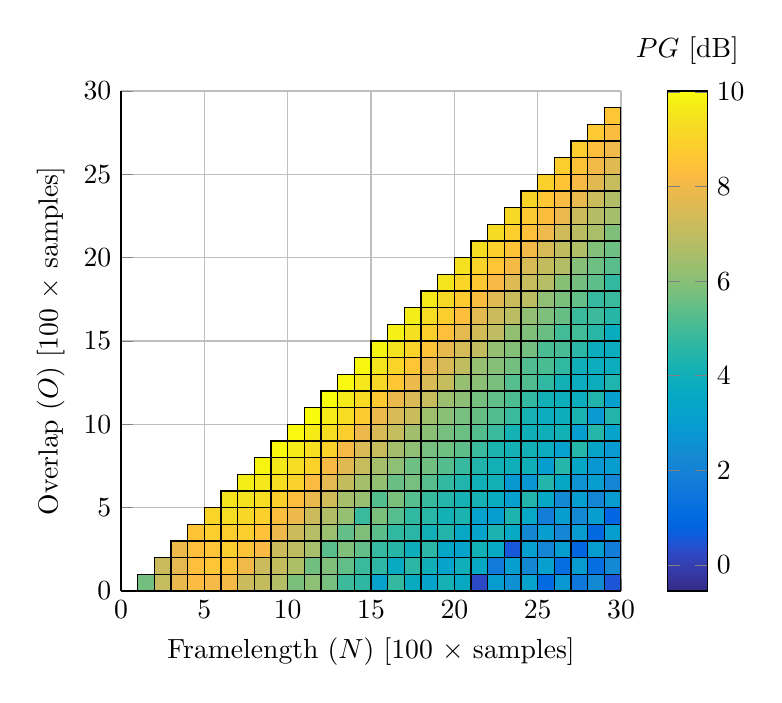
\begin{tikzpicture}


\begin{axis}[%
width=2.5in,
height=2.5in,
scale only axis,
point meta min=-0.551769511455843,
point meta max=10.0207598959184,
unbounded coords=jump,
xmin=0,
xmax=3000,
xlabel={Framelength ($N$) [100 $\times$ samples]},
xmajorgrids,
ymin=0,
ymax=3000,
ytick={0,500,...,3000},
yticklabels={0,5,...,30},
xtick={0,500,...,3000},
xticklabels={0,5,...,30},
ylabel={Overlap ($O$) [100 $\times$ samples]},
ymajorgrids,
axis background/.style={fill=white},
axis x line*=bottom,
axis y line*=left,
colormap={mymap}{[1pt] rgb(0pt)=(0.2081,0.1663,0.5292); rgb(1pt)=(0.211624,0.189781,0.577676); rgb(2pt)=(0.212252,0.213771,0.626971); rgb(3pt)=(0.2081,0.2386,0.677086); rgb(4pt)=(0.195905,0.264457,0.7279); rgb(5pt)=(0.170729,0.291938,0.779248); rgb(6pt)=(0.125271,0.324243,0.830271); rgb(7pt)=(0.0591333,0.359833,0.868333); rgb(8pt)=(0.0116952,0.38751,0.881957); rgb(9pt)=(0.00595714,0.408614,0.882843); rgb(10pt)=(0.0165143,0.4266,0.878633); rgb(11pt)=(0.0328524,0.443043,0.871957); rgb(12pt)=(0.0498143,0.458571,0.864057); rgb(13pt)=(0.0629333,0.47369,0.855438); rgb(14pt)=(0.0722667,0.488667,0.8467); rgb(15pt)=(0.0779429,0.503986,0.838371); rgb(16pt)=(0.0793476,0.520024,0.831181); rgb(17pt)=(0.0749429,0.537543,0.826271); rgb(18pt)=(0.0640571,0.556986,0.823957); rgb(19pt)=(0.0487714,0.577224,0.822829); rgb(20pt)=(0.0343429,0.596581,0.819852); rgb(21pt)=(0.0265,0.6137,0.8135); rgb(22pt)=(0.0238905,0.628662,0.803762); rgb(23pt)=(0.0230905,0.641786,0.791267); rgb(24pt)=(0.0227714,0.653486,0.776757); rgb(25pt)=(0.0266619,0.664195,0.760719); rgb(26pt)=(0.0383714,0.674271,0.743552); rgb(27pt)=(0.0589714,0.683757,0.725386); rgb(28pt)=(0.0843,0.692833,0.706167); rgb(29pt)=(0.113295,0.7015,0.685857); rgb(30pt)=(0.145271,0.709757,0.664629); rgb(31pt)=(0.180133,0.717657,0.642433); rgb(32pt)=(0.217829,0.725043,0.619262); rgb(33pt)=(0.258643,0.731714,0.595429); rgb(34pt)=(0.302171,0.737605,0.571186); rgb(35pt)=(0.348167,0.742433,0.547267); rgb(36pt)=(0.395257,0.7459,0.524443); rgb(37pt)=(0.44201,0.748081,0.503314); rgb(38pt)=(0.487124,0.749062,0.483976); rgb(39pt)=(0.530029,0.749114,0.466114); rgb(40pt)=(0.570857,0.748519,0.44939); rgb(41pt)=(0.609852,0.747314,0.433686); rgb(42pt)=(0.6473,0.7456,0.4188); rgb(43pt)=(0.683419,0.743476,0.404433); rgb(44pt)=(0.71841,0.741133,0.390476); rgb(45pt)=(0.752486,0.7384,0.376814); rgb(46pt)=(0.785843,0.735567,0.363271); rgb(47pt)=(0.818505,0.732733,0.34979); rgb(48pt)=(0.850657,0.7299,0.336029); rgb(49pt)=(0.882433,0.727433,0.3217); rgb(50pt)=(0.913933,0.725786,0.306276); rgb(51pt)=(0.944957,0.726114,0.288643); rgb(52pt)=(0.973895,0.731395,0.266648); rgb(53pt)=(0.993771,0.745457,0.240348); rgb(54pt)=(0.999043,0.765314,0.216414); rgb(55pt)=(0.995533,0.786057,0.196652); rgb(56pt)=(0.988,0.8066,0.179367); rgb(57pt)=(0.978857,0.827143,0.163314); rgb(58pt)=(0.9697,0.848138,0.147452); rgb(59pt)=(0.962586,0.870514,0.1309); rgb(60pt)=(0.958871,0.8949,0.113243); rgb(61pt)=(0.959824,0.921833,0.0948381); rgb(62pt)=(0.9661,0.951443,0.0755333); rgb(63pt)=(0.9763,0.9831,0.0538)},
colorbar,
colorbar style={title=$PG$ [dB]}
]%ylabel={PG}

\addplot[%
surf,
opacity = ceil(\pgfplotspointmetatransformed),
shader=flat corner,draw=black,colormap={mymap}{[1pt] rgb(0pt)=(0.2081,0.1663,0.5292); rgb(1pt)=(0.211624,0.189781,0.577676); rgb(2pt)=(0.212252,0.213771,0.626971); rgb(3pt)=(0.2081,0.2386,0.677086); rgb(4pt)=(0.195905,0.264457,0.7279); rgb(5pt)=(0.170729,0.291938,0.779248); rgb(6pt)=(0.125271,0.324243,0.830271); rgb(7pt)=(0.0591333,0.359833,0.868333); rgb(8pt)=(0.0116952,0.38751,0.881957); rgb(9pt)=(0.00595714,0.408614,0.882843); rgb(10pt)=(0.0165143,0.4266,0.878633); rgb(11pt)=(0.0328524,0.443043,0.871957); rgb(12pt)=(0.0498143,0.458571,0.864057); rgb(13pt)=(0.0629333,0.47369,0.855438); rgb(14pt)=(0.0722667,0.488667,0.8467); rgb(15pt)=(0.0779429,0.503986,0.838371); rgb(16pt)=(0.0793476,0.520024,0.831181); rgb(17pt)=(0.0749429,0.537543,0.826271); rgb(18pt)=(0.0640571,0.556986,0.823957); rgb(19pt)=(0.0487714,0.577224,0.822829); rgb(20pt)=(0.0343429,0.596581,0.819852); rgb(21pt)=(0.0265,0.6137,0.8135); rgb(22pt)=(0.0238905,0.628662,0.803762); rgb(23pt)=(0.0230905,0.641786,0.791267); rgb(24pt)=(0.0227714,0.653486,0.776757); rgb(25pt)=(0.0266619,0.664195,0.760719); rgb(26pt)=(0.0383714,0.674271,0.743552); rgb(27pt)=(0.0589714,0.683757,0.725386); rgb(28pt)=(0.0843,0.692833,0.706167); rgb(29pt)=(0.113295,0.7015,0.685857); rgb(30pt)=(0.145271,0.709757,0.664629); rgb(31pt)=(0.180133,0.717657,0.642433); rgb(32pt)=(0.217829,0.725043,0.619262); rgb(33pt)=(0.258643,0.731714,0.595429); rgb(34pt)=(0.302171,0.737605,0.571186); rgb(35pt)=(0.348167,0.742433,0.547267); rgb(36pt)=(0.395257,0.7459,0.524443); rgb(37pt)=(0.44201,0.748081,0.503314); rgb(38pt)=(0.487124,0.749062,0.483976); rgb(39pt)=(0.530029,0.749114,0.466114); rgb(40pt)=(0.570857,0.748519,0.44939); rgb(41pt)=(0.609852,0.747314,0.433686); rgb(42pt)=(0.6473,0.7456,0.4188); rgb(43pt)=(0.683419,0.743476,0.404433); rgb(44pt)=(0.71841,0.741133,0.390476); rgb(45pt)=(0.752486,0.7384,0.376814); rgb(46pt)=(0.785843,0.735567,0.363271); rgb(47pt)=(0.818505,0.732733,0.34979); rgb(48pt)=(0.850657,0.7299,0.336029); rgb(49pt)=(0.882433,0.727433,0.3217); rgb(50pt)=(0.913933,0.725786,0.306276); rgb(51pt)=(0.944957,0.726114,0.288643); rgb(52pt)=(0.973895,0.731395,0.266648); rgb(53pt)=(0.993771,0.745457,0.240348); rgb(54pt)=(0.999043,0.765314,0.216414); rgb(55pt)=(0.995533,0.786057,0.196652); rgb(56pt)=(0.988,0.8066,0.179367); rgb(57pt)=(0.978857,0.827143,0.163314); rgb(58pt)=(0.9697,0.848138,0.147452); rgb(59pt)=(0.962586,0.870514,0.1309); rgb(60pt)=(0.958871,0.8949,0.113243); rgb(61pt)=(0.959824,0.921833,0.0948381); rgb(62pt)=(0.9661,0.951443,0.0755333); rgb(63pt)=(0.9763,0.9831,0.0538)},mesh/rows=30]
table[row sep=crcr, point meta=\thisrow{c}] {%
%
x	y	c\\
100	0	5.6827458135075\\
100	100	nan\\
100	200	nan\\
100	300	nan\\
100	400	nan\\
100	500	nan\\
100	600	nan\\
100	700	nan\\
100	800	nan\\
100	900	nan\\
100	1000	nan\\
100	1100	nan\\
100	1200	nan\\
100	1300	nan\\
100	1400	nan\\
100	1500	nan\\
100	1600	nan\\
100	1700	nan\\
100	1800	nan\\
100	1900	nan\\
100	2000	nan\\
100	2100	nan\\
100	2200	nan\\
100	2300	nan\\
100	2400	nan\\
100	2500	nan\\
100	2600	nan\\
100	2700	nan\\
100	2800	nan\\
100	2900	nan\\
200	0	7.0790317182078\\
200	100	7.18389489543295\\
200	200	nan\\
200	300	nan\\
200	400	nan\\
200	500	nan\\
200	600	nan\\
200	700	nan\\
200	800	nan\\
200	900	nan\\
200	1000	nan\\
200	1100	nan\\
200	1200	nan\\
200	1300	nan\\
200	1400	nan\\
200	1500	nan\\
200	1600	nan\\
200	1700	nan\\
200	1800	nan\\
200	1900	nan\\
200	2000	nan\\
200	2100	nan\\
200	2200	nan\\
200	2300	nan\\
200	2400	nan\\
200	2500	nan\\
200	2600	nan\\
200	2700	nan\\
200	2800	nan\\
200	2900	nan\\
300	0	7.8278797182668\\
300	100	7.75061670667307\\
300	200	7.94964232573768\\
300	300	nan\\
300	400	nan\\
300	500	nan\\
300	600	nan\\
300	700	nan\\
300	800	nan\\
300	900	nan\\
300	1000	nan\\
300	1100	nan\\
300	1200	nan\\
300	1300	nan\\
300	1400	nan\\
300	1500	nan\\
300	1600	nan\\
300	1700	nan\\
300	1800	nan\\
300	1900	nan\\
300	2000	nan\\
300	2100	nan\\
300	2200	nan\\
300	2300	nan\\
300	2400	nan\\
300	2500	nan\\
300	2600	nan\\
300	2700	nan\\
300	2800	nan\\
300	2900	nan\\
400	0	8.25982045157361\\
400	100	8.37365829237133\\
400	200	8.38994845512447\\
400	300	8.53395155897113\\
400	400	nan\\
400	500	nan\\
400	600	nan\\
400	700	nan\\
400	800	nan\\
400	900	nan\\
400	1000	nan\\
400	1100	nan\\
400	1200	nan\\
400	1300	nan\\
400	1400	nan\\
400	1500	nan\\
400	1600	nan\\
400	1700	nan\\
400	1800	nan\\
400	1900	nan\\
400	2000	nan\\
400	2100	nan\\
400	2200	nan\\
400	2300	nan\\
400	2400	nan\\
400	2500	nan\\
400	2600	nan\\
400	2700	nan\\
400	2800	nan\\
400	2900	nan\\
500	0	8.09522110947221\\
500	100	8.58404936019439\\
500	200	8.52476852167647\\
500	300	8.85395289600773\\
500	400	9.03400135477561\\
500	500	nan\\
500	600	nan\\
500	700	nan\\
500	800	nan\\
500	900	nan\\
500	1000	nan\\
500	1100	nan\\
500	1200	nan\\
500	1300	nan\\
500	1400	nan\\
500	1500	nan\\
500	1600	nan\\
500	1700	nan\\
500	1800	nan\\
500	1900	nan\\
500	2000	nan\\
500	2100	nan\\
500	2200	nan\\
500	2300	nan\\
500	2400	nan\\
500	2500	nan\\
500	2600	nan\\
500	2700	nan\\
500	2800	nan\\
500	2900	nan\\
600	0	8.05650724153339\\
600	100	8.54693570913705\\
600	200	8.8377683265956\\
600	300	8.82559971223848\\
600	400	9.28658312212634\\
600	500	9.52161535433559\\
600	600	nan\\
600	700	nan\\
600	800	nan\\
600	900	nan\\
600	1000	nan\\
600	1100	nan\\
600	1200	nan\\
600	1300	nan\\
600	1400	nan\\
600	1500	nan\\
600	1600	nan\\
600	1700	nan\\
600	1800	nan\\
600	1900	nan\\
600	2000	nan\\
600	2100	nan\\
600	2200	nan\\
600	2300	nan\\
600	2400	nan\\
600	2500	nan\\
600	2600	nan\\
600	2700	nan\\
600	2800	nan\\
600	2900	nan\\
700	0	7.20736652003549\\
700	100	8.01860060821804\\
700	200	8.5092217869215\\
700	300	8.85498614721321\\
700	400	9.13100370114176\\
700	500	9.43150883603405\\
700	600	9.74782220562509\\
700	700	nan\\
700	800	nan\\
700	900	nan\\
700	1000	nan\\
700	1100	nan\\
700	1200	nan\\
700	1300	nan\\
700	1400	nan\\
700	1500	nan\\
700	1600	nan\\
700	1700	nan\\
700	1800	nan\\
700	1900	nan\\
700	2000	nan\\
700	2100	nan\\
700	2200	nan\\
700	2300	nan\\
700	2400	nan\\
700	2500	nan\\
700	2600	nan\\
700	2700	nan\\
700	2800	nan\\
700	2900	nan\\
800	0	7.06129617908756\\
800	100	7.21625389795336\\
800	200	8.17024678080842\\
800	300	8.4506398874489\\
800	400	8.92543148972206\\
800	500	9.31059383665309\\
800	600	9.57358732259701\\
800	700	9.88474425342921\\
800	800	nan\\
800	900	nan\\
800	1000	nan\\
800	1100	nan\\
800	1200	nan\\
800	1300	nan\\
800	1400	nan\\
800	1500	nan\\
800	1600	nan\\
800	1700	nan\\
800	1800	nan\\
800	1900	nan\\
800	2000	nan\\
800	2100	nan\\
800	2200	nan\\
800	2300	nan\\
800	2400	nan\\
800	2500	nan\\
800	2600	nan\\
800	2700	nan\\
800	2800	nan\\
800	2900	nan\\
900	0	6.7603240209297\\
900	100	7.07027516643772\\
900	200	7.21503157848168\\
900	300	7.91680228410601\\
900	400	8.33413384154289\\
900	500	8.91700110520262\\
900	600	9.33441266257382\\
900	700	9.61050000584357\\
900	800	9.96602273571317\\
900	900	nan\\
900	1000	nan\\
900	1100	nan\\
900	1200	nan\\
900	1300	nan\\
900	1400	nan\\
900	1500	nan\\
900	1600	nan\\
900	1700	nan\\
900	1800	nan\\
900	1900	nan\\
900	2000	nan\\
900	2100	nan\\
900	2200	nan\\
900	2300	nan\\
900	2400	nan\\
900	2500	nan\\
900	2600	nan\\
900	2700	nan\\
900	2800	nan\\
900	2900	nan\\
1000	0	5.79141266758575\\
1000	100	6.6583846543796\\
1000	200	6.96560213501504\\
1000	300	7.24068731658401\\
1000	400	7.9395591224285\\
1000	500	8.31867811054653\\
1000	600	8.9754932003346\\
1000	700	9.34845065231673\\
1000	800	9.67344129050852\\
1000	900	9.99470564606262\\
1000	1000	nan\\
1000	1100	nan\\
1000	1200	nan\\
1000	1300	nan\\
1000	1400	nan\\
1000	1500	nan\\
1000	1600	nan\\
1000	1700	nan\\
1000	1800	nan\\
1000	1900	nan\\
1000	2000	nan\\
1000	2100	nan\\
1000	2200	nan\\
1000	2300	nan\\
1000	2400	nan\\
1000	2500	nan\\
1000	2600	nan\\
1000	2700	nan\\
1000	2800	nan\\
1000	2900	nan\\
1100	0	6.08510006030311\\
1100	100	5.66131684642677\\
1100	200	6.52494101151453\\
1100	300	6.8154749961067\\
1100	400	7.2221683246724\\
1100	500	7.85272239575603\\
1100	600	8.25834444268623\\
1100	700	8.98246828788382\\
1100	800	9.38384280669374\\
1100	900	9.67888280713376\\
1100	1000	10.0207598959184\\
1100	1100	nan\\
1100	1200	nan\\
1100	1300	nan\\
1100	1400	nan\\
1100	1500	nan\\
1100	1600	nan\\
1100	1700	nan\\
1100	1800	nan\\
1100	1900	nan\\
1100	2000	nan\\
1100	2100	nan\\
1100	2200	nan\\
1100	2300	nan\\
1100	2400	nan\\
1100	2500	nan\\
1100	2600	nan\\
1100	2700	nan\\
1100	2800	nan\\
1100	2900	nan\\
1200	0	5.75236385929885\\
1200	100	5.8893978793085\\
1200	200	5.3233876826882\\
1200	300	6.30245671838949\\
1200	400	6.70416183583482\\
1200	500	7.29231639499116\\
1200	600	7.73083236703484\\
1200	700	8.13278866080154\\
1200	800	8.95016901139914\\
1200	900	9.3575654964583\\
1200	1000	9.69962351631871\\
1200	1100	10.018452727616\\
1200	1200	nan\\
1200	1300	nan\\
1200	1400	nan\\
1200	1500	nan\\
1200	1600	nan\\
1200	1700	nan\\
1200	1800	nan\\
1200	1900	nan\\
1200	2000	nan\\
1200	2100	nan\\
1200	2200	nan\\
1200	2300	nan\\
1200	2400	nan\\
1200	2500	nan\\
1200	2600	nan\\
1200	2700	nan\\
1200	2800	nan\\
1200	2900	nan\\
1300	0	4.8910628019805\\
1300	100	5.45072016874233\\
1300	200	5.86850066777867\\
1300	300	5.4597166268533\\
1300	400	6.21490882072339\\
1300	500	6.48849191466192\\
1300	600	7.05573401013256\\
1300	700	7.66870480877405\\
1300	800	8.12020714201073\\
1300	900	8.84241536316059\\
1300	1000	9.32521343768448\\
1300	1100	9.66682615033229\\
1300	1200	9.99393859933556\\
1300	1300	nan\\
1300	1400	nan\\
1300	1500	nan\\
1300	1600	nan\\
1300	1700	nan\\
1300	1800	nan\\
1300	1900	nan\\
1300	2000	nan\\
1300	2100	nan\\
1300	2200	nan\\
1300	2300	nan\\
1300	2400	nan\\
1300	2500	nan\\
1300	2600	nan\\
1300	2700	nan\\
1300	2800	nan\\
1300	2900	nan\\
1400	0	4.68328180207416\\
1400	100	4.87031890586883\\
1400	200	5.46124064783872\\
1400	300	5.87957713868692\\
1400	400	4.86401495955569\\
1400	500	6.26391766665361\\
1400	600	6.48566475687751\\
1400	700	7.13851035956643\\
1400	800	7.50027034876972\\
1400	900	7.94746340189027\\
1400	1000	8.77453134934714\\
1400	1100	9.23762319980819\\
1400	1200	9.58536439829166\\
1400	1300	9.93647418346277\\
1400	1400	nan\\
1400	1500	nan\\
1400	1600	nan\\
1400	1700	nan\\
1400	1800	nan\\
1400	1900	nan\\
1400	2000	nan\\
1400	2100	nan\\
1400	2200	nan\\
1400	2300	nan\\
1400	2400	nan\\
1400	2500	nan\\
1400	2600	nan\\
1400	2700	nan\\
1400	2800	nan\\
1400	2900	nan\\
1500	0	3.24765243794076\\
1500	100	4.65481232593174\\
1500	200	4.79830988957897\\
1500	300	5.35751567095906\\
1500	400	5.79287838471904\\
1500	500	5.25522140259071\\
1500	600	6.17072553135157\\
1500	700	6.48214041903959\\
1500	800	7.1345332299744\\
1500	900	7.48068047659614\\
1500	1000	7.89377405226484\\
1500	1100	8.70610504087698\\
1500	1200	9.16324372984275\\
1500	1300	9.52474035946379\\
1500	1400	9.86030813520319\\
1500	1500	nan\\
1500	1600	nan\\
1500	1700	nan\\
1500	1800	nan\\
1500	1900	nan\\
1500	2000	nan\\
1500	2100	nan\\
1500	2200	nan\\
1500	2300	nan\\
1500	2400	nan\\
1500	2500	nan\\
1500	2600	nan\\
1500	2700	nan\\
1500	2800	nan\\
1500	2900	nan\\
1600	0	4.75276003383697\\
1600	100	3.67495640572055\\
1600	200	4.52251715002299\\
1600	300	4.70771251796696\\
1600	400	5.26201893473007\\
1600	500	5.81200015855313\\
1600	600	5.54198269350814\\
1600	700	6.09112217072302\\
1600	800	6.43437379918348\\
1600	900	7.09943797512656\\
1600	1000	7.48241897845622\\
1600	1100	7.90693168041642\\
1600	1200	8.6380368658202\\
1600	1300	9.0916878406797\\
1600	1400	9.45586978035725\\
1600	1500	9.79114079162636\\
1600	1600	nan\\
1600	1700	nan\\
1600	1800	nan\\
1600	1900	nan\\
1600	2000	nan\\
1600	2100	nan\\
1600	2200	nan\\
1600	2300	nan\\
1600	2400	nan\\
1600	2500	nan\\
1600	2600	nan\\
1600	2700	nan\\
1600	2800	nan\\
1600	2900	nan\\
1700	0	3.71748664243527\\
1700	100	4.60591980476924\\
1700	200	3.91362630267876\\
1700	300	4.55847242510564\\
1700	400	4.70161157949911\\
1700	500	5.26688872672145\\
1700	600	5.74077415219596\\
1700	700	5.60918413969161\\
1700	800	6.12512258839059\\
1700	900	6.40152380276071\\
1700	1000	7.16577614393491\\
1700	1100	7.4954835376692\\
1700	1200	7.90408510720934\\
1700	1300	8.57357709454054\\
1700	1400	9.0277543415418\\
1700	1500	9.3764265164728\\
1700	1600	9.7243052974142\\
1700	1700	nan\\
1700	1800	nan\\
1700	1900	nan\\
1700	2000	nan\\
1700	2100	nan\\
1700	2200	nan\\
1700	2300	nan\\
1700	2400	nan\\
1700	2500	nan\\
1700	2600	nan\\
1700	2700	nan\\
1700	2800	nan\\
1700	2900	nan\\
1800	0	3.3177087556264\\
1800	100	4.01520154764494\\
1800	200	4.58897692120239\\
1800	300	4.05120880760072\\
1800	400	4.53307279512351\\
1800	500	4.80647025338146\\
1800	600	5.30764576164913\\
1800	700	5.66202006578872\\
1800	800	5.75312164595155\\
1800	900	6.04395256930141\\
1800	1000	6.3700405132766\\
1800	1100	7.14316992342896\\
1800	1200	7.48470310198768\\
1800	1300	7.87037714378024\\
1800	1400	8.48717243248572\\
1800	1500	8.92938209706209\\
1800	1600	9.3014704008889\\
1800	1700	9.64275886586559\\
1800	1800	nan\\
1800	1900	nan\\
1800	2000	nan\\
1800	2100	nan\\
1800	2200	nan\\
1800	2300	nan\\
1800	2400	nan\\
1800	2500	nan\\
1800	2600	nan\\
1800	2700	nan\\
1800	2800	nan\\
1800	2900	nan\\
1900	0	4.16438107268957\\
1900	100	3.30621453732177\\
1900	200	3.45177011062336\\
1900	300	4.41976545924296\\
1900	400	4.07826463673203\\
1900	500	4.47250181773447\\
1900	600	4.74401157157616\\
1900	700	5.27110068830706\\
1900	800	5.6301314654757\\
1900	900	5.74823980250472\\
1900	1000	6.03395598979113\\
1900	1100	6.3316791328726\\
1900	1200	7.11053211593739\\
1900	1300	7.45923534882344\\
1900	1400	7.81374082935247\\
1900	1500	8.40334989731675\\
1900	1600	8.81911874169977\\
1900	1700	9.19800880789435\\
1900	1800	9.54583520361966\\
1900	1900	nan\\
1900	2000	nan\\
1900	2100	nan\\
1900	2200	nan\\
1900	2300	nan\\
1900	2400	nan\\
1900	2500	nan\\
1900	2600	nan\\
1900	2700	nan\\
1900	2800	nan\\
1900	2900	nan\\
2000	0	3.63837130417713\\
2000	100	3.96838494244702\\
2000	200	3.28360542391229\\
2000	300	3.55278143786063\\
2000	400	4.26805123856089\\
2000	500	4.15389920807166\\
2000	600	4.39329679744196\\
2000	700	4.78828316129288\\
2000	800	5.37993737198608\\
2000	900	5.58147465390246\\
2000	1000	5.7286955025126\\
2000	1100	6.07285315548354\\
2000	1200	6.23857857671884\\
2000	1300	7.01013622331059\\
2000	1400	7.40631428562525\\
2000	1500	7.74343597295201\\
2000	1600	8.32757229622458\\
2000	1700	8.74188942454939\\
2000	1800	9.09209523315045\\
2000	1900	9.44134118935649\\
2000	2000	nan\\
2000	2100	nan\\
2000	2200	nan\\
2000	2300	nan\\
2000	2400	nan\\
2000	2500	nan\\
2000	2600	nan\\
2000	2700	nan\\
2000	2800	nan\\
2000	2900	nan\\
2100	0	0.264623542453294\\
2100	100	3.63488656288565\\
2100	200	4.08913120930422\\
2100	300	3.28220109142383\\
2100	400	3.18039510652367\\
2100	500	4.19474057968373\\
2100	600	4.0275612369305\\
2100	700	4.39427002201494\\
2100	800	4.86473111214704\\
2100	900	5.25381195203792\\
2100	1000	5.52645898428144\\
2100	1100	5.71270454803943\\
2100	1200	6.05580569501984\\
2100	1300	6.23707654312965\\
2100	1400	7.00000513992408\\
2100	1500	7.3381894461935\\
2100	1600	7.70510502361266\\
2100	1700	8.27878784954097\\
2100	1800	8.66979451640054\\
2100	1900	9.0155911617751\\
2100	2000	9.34506416881835\\
2100	2100	nan\\
2100	2200	nan\\
2100	2300	nan\\
2100	2400	nan\\
2100	2500	nan\\
2100	2600	nan\\
2100	2700	nan\\
2100	2800	nan\\
2100	2900	nan\\
2200	0	2.95170309874089\\
2200	100	1.73360893357364\\
2200	200	3.61323080676111\\
2200	300	4.28061341062458\\
2200	400	3.02458697343151\\
2200	500	3.75811713713825\\
2200	600	4.06218778116715\\
2200	700	4.05610248843421\\
2200	800	4.30007538322245\\
2200	900	4.85697872751457\\
2200	1000	5.22977855686604\\
2200	1100	5.42728488717261\\
2200	1200	5.7742976825497\\
2200	1300	5.9578809065615\\
2200	1400	6.20369481654021\\
2200	1500	6.97748546317166\\
2200	1600	7.25905430947499\\
2200	1700	7.63071051415358\\
2200	1800	8.17187520251639\\
2200	1900	8.56846748612261\\
2200	2000	8.92936194092831\\
2200	2100	9.25326090597395\\
2200	2200	nan\\
2200	2300	nan\\
2200	2400	nan\\
2200	2500	nan\\
2200	2600	nan\\
2200	2700	nan\\
2200	2800	nan\\
2200	2900	nan\\
2300	0	2.53293217519118\\
2300	100	3.00938026182184\\
2300	200	0.551769511455843\\
2300	300	3.60726664380354\\
2300	400	4.36229780994093\\
2300	500	3.08643225262487\\
2300	600	2.82564622459287\\
2300	700	3.98306729613317\\
2300	800	4.11490314132238\\
2300	900	4.13618785976634\\
2300	1000	4.86317380717345\\
2300	1100	5.16517700158233\\
2300	1200	5.26664183435126\\
2300	1300	5.69684803139814\\
2300	1400	5.95135216558113\\
2300	1500	6.16719875147937\\
2300	1600	6.89154945837155\\
2300	1700	7.18393537254356\\
2300	1800	7.60032386475286\\
2300	1900	8.1060139824226\\
2300	2000	8.49168618698787\\
2300	2100	8.84145695288964\\
2300	2200	9.16963549024874\\
2300	2300	nan\\
2300	2400	nan\\
2300	2500	nan\\
2300	2600	nan\\
2300	2700	nan\\
2300	2800	nan\\
2300	2900	nan\\
2400	0	3.23692740006642\\
2400	100	2.2228524336536\\
2400	200	3.08472299555247\\
2400	300	2.2240377386973\\
2400	400	3.53887086816519\\
2400	500	4.42615653537038\\
2400	600	2.75840359129067\\
2400	700	4.0107386280573\\
2400	800	4.05214769333313\\
2400	900	4.00914531419853\\
2400	1000	4.17937149969251\\
2400	1100	4.74117848303689\\
2400	1200	5.2085286363726\\
2400	1300	5.19304330014419\\
2400	1400	5.69847355162021\\
2400	1500	5.87188705075393\\
2400	1600	6.15489171474828\\
2400	1700	6.89765995399639\\
2400	1800	7.11879031436815\\
2400	1900	7.49046026449902\\
2400	2000	8.04502341053814\\
2400	2100	8.40465258616035\\
2400	2200	8.73328129071907\\
2400	2300	9.06128194950849\\
2400	2400	nan\\
2400	2500	nan\\
2400	2600	nan\\
2400	2700	nan\\
2400	2800	nan\\
2400	2900	nan\\
2500	0	1.05000257678802\\
2500	100	3.09955807465487\\
2500	200	2.13019145244393\\
2500	300	2.98129659738565\\
2500	400	1.80823551110839\\
2500	500	3.44295461285468\\
2500	600	4.45023506033534\\
2500	700	3.03486862485067\\
2500	800	3.799754032993\\
2500	900	3.97648541270297\\
2500	1000	3.83352254491892\\
2500	1100	4.04591105923088\\
2500	1200	4.69567516678935\\
2500	1300	5.11099504335296\\
2500	1400	5.09859465247581\\
2500	1500	5.57858218898721\\
2500	1600	5.8569467833986\\
2500	1700	6.10341874446816\\
2500	1800	6.81391868519097\\
2500	1900	7.03573319906174\\
2500	2000	7.42018466644079\\
2500	2100	7.9589647003702\\
2500	2200	8.29921705504155\\
2500	2300	8.63637971004693\\
2500	2400	8.96380635737141\\
2500	2500	nan\\
2500	2600	nan\\
2500	2700	nan\\
2500	2800	nan\\
2500	2900	nan\\
2600	0	2.80208415075651\\
2600	100	1.17194843956108\\
2600	200	2.96109260453396\\
2600	300	2.19270843592341\\
2600	400	3.0115728867441\\
2600	500	2.28393968299924\\
2600	600	3.47369768467374\\
2600	700	4.50853743880052\\
2600	800	3.15812371844604\\
2600	900	4.07856863803736\\
2600	1000	3.91468626002954\\
2600	1100	3.89808210094217\\
2600	1200	4.04567753651072\\
2600	1300	4.70566985097843\\
2600	1400	5.07194378908158\\
2600	1500	4.99752267777982\\
2600	1600	5.52550384847648\\
2600	1700	5.79174211203976\\
2600	1800	6.00046246850643\\
2600	1900	6.74511848933576\\
2600	2000	6.98699179435392\\
2600	2100	7.31013917497011\\
2600	2200	7.87653800818457\\
2600	2300	8.22494050640918\\
2600	2400	8.54322091765009\\
2600	2500	8.85820789226427\\
2600	2600	nan\\
2600	2700	nan\\
2600	2800	nan\\
2600	2900	nan\\
2700	0	1.58184394833386\\
2700	100	2.92525400331244\\
2700	200	0.887359676794604\\
2700	300	2.93101822389555\\
2700	400	2.30024404624266\\
2700	500	3.00032580576816\\
2700	600	2.58705024710389\\
2700	700	3.44496986930798\\
2700	800	4.4916042025927\\
2700	900	2.98522379998911\\
2700	1000	4.25749977657229\\
2700	1100	3.87067312264047\\
2700	1200	3.83784894949447\\
2700	1300	3.98929857887126\\
2700	1400	4.59197088590304\\
2700	1500	4.99312405800586\\
2700	1600	4.86180118194934\\
2700	1700	5.46261986535732\\
2700	1800	5.70973165052257\\
2700	1900	5.97276788996415\\
2700	2000	6.67403857872095\\
2700	2100	6.91286174850295\\
2700	2200	7.25280658811363\\
2700	2300	7.81626379934614\\
2700	2400	8.13648239969618\\
2700	2500	8.46913649633422\\
2700	2600	8.78457026475621\\
2700	2700	nan\\
2700	2800	nan\\
2700	2900	nan\\
2800	0	2.2987560540242\\
2800	100	1.19896433152671\\
2800	200	2.95163573066064\\
2800	300	0.973202079270705\\
2800	400	2.97370455963156\\
2800	500	2.12856324963795\\
2800	600	2.98222869928969\\
2800	700	2.77033362268512\\
2800	800	3.38784440474213\\
2800	900	4.50283031414694\\
2800	1000	2.86687295264398\\
2800	1100	4.3797702935594\\
2800	1200	3.86077604223459\\
2800	1300	3.88445747215116\\
2800	1400	3.88641891122799\\
2800	1500	4.54099461834347\\
2800	1600	4.89171252973565\\
2800	1700	4.80102017502878\\
2800	1800	5.38055416094404\\
2800	1900	5.62096395390293\\
2800	2000	5.9064550594499\\
2800	2100	6.57396144817971\\
2800	2200	6.77884258803287\\
2800	2300	7.20159987892983\\
2800	2400	7.70137646156138\\
2800	2500	8.02001565102648\\
2800	2600	8.3537017651593\\
2800	2700	8.6861911739627\\
2800	2800	nan\\
2800	2900	nan\\
2900	0	0.49312967237007\\
2900	100	2.25840014462245\\
2900	200	1.80380427347787\\
2900	300	3.03746280090745\\
2900	400	0.845717353642782\\
2900	500	2.91980222011896\\
2900	600	2.20120210963457\\
2900	700	2.99077861803715\\
2900	800	2.87641657842737\\
2900	900	3.26134076790394\\
2900	1000	4.42889490862495\\
2900	1100	3.07565824698724\\
2900	1200	4.36835391429797\\
2900	1300	3.8835622884345\\
2900	1400	3.84533451378335\\
2900	1500	3.78342493811934\\
2900	1600	4.5195926660129\\
2900	1700	4.84979739867748\\
2900	1800	4.72342685477777\\
2900	1900	5.32512315595608\\
2900	2000	5.60997138907586\\
2900	2100	5.87473951276466\\
2900	2200	6.48270953309765\\
2900	2300	6.71059287812374\\
2900	2400	7.1263819393935\\
2900	2500	7.63768597628047\\
2900	2600	7.95785638792816\\
2900	2700	8.27184455059282\\
2900	2800	8.58887864737359\\
2900	2900	nan\\
3000	0	-0.084166652386565\\
3000	100	0.658799202686103\\
3000	200	2.4286786445431\\
3000	300	2.00173215444182\\
3000	400	3.04605438638216\\
3000	500	0.804121831033953\\
3000	600	2.80060747061573\\
3000	700	2.10723369617921\\
3000	800	3.00606491677149\\
3000	900	2.9921027849289\\
3000	1000	3.2003941437714\\
3000	1100	4.47914328347861\\
3000	1200	3.09026222985996\\
3000	1300	4.40877799382241\\
3000	1400	3.86783693309201\\
3000	1500	3.82141825431614\\
3000	1600	3.75968653309083\\
3000	1700	4.42136187911435\\
3000	1800	4.73062760871956\\
3000	1900	4.65092537646692\\
3000	2000	5.26464935536502\\
3000	2100	5.53276290699877\\
3000	2200	5.79426518264794\\
3000	2300	6.43034113528171\\
3000	2400	6.61621727344431\\
3000	2500	6.98815251985862\\
3000	2600	7.51974760550906\\
3000	2700	7.84037752158828\\
3000	2800	8.1530922590658\\
3000	2900	8.49883156713133\\
};
\end{axis}
\end{tikzpicture}%}
	\end{column}
\end{columns}
\end{frame}

\begin{frame}{Simulation Results}{Optimal parameters}		
\begin{columns}
	\begin{column}{0.4\textwidth}
	\begin{itemize}
		\item Prediction order P = 4
		\item Optimal parameters
		\begin{itemize}
			\item Framelength N = 300
			\item Overlap O = 250
		\end{itemize}
		\item Prediction Gain PG = ??? dB
	\end{itemize}
	\end{column}
	\begin{column}{0.6\textwidth} 
		\resizebox{0.9\columnwidth}{!}{		
			% This file was created by matlab2tikz.
%
%The latest updates can be retrieved from
%  http://www.mathworks.com/matlabcentral/fileexchange/22022-matlab2tikz-matlab2tikz
%where you can also make suggestions and rate matlab2tikz.
%
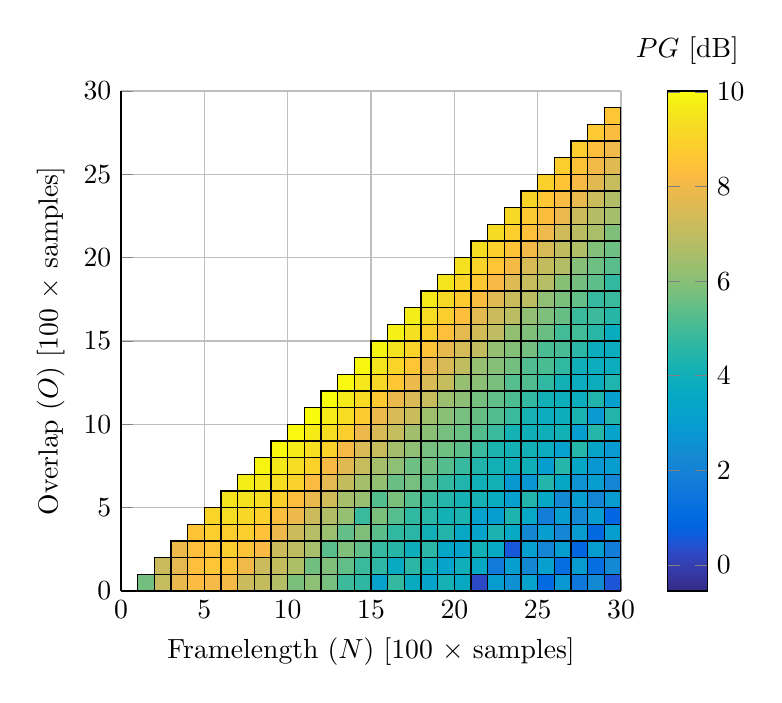
\begin{tikzpicture}


\begin{axis}[%
width=2.5in,
height=2.5in,
scale only axis,
point meta min=-0.551769511455843,
point meta max=10.0207598959184,
unbounded coords=jump,
xmin=0,
xmax=3000,
xlabel={Framelength ($N$) [100 $\times$ samples]},
xmajorgrids,
ymin=0,
ymax=3000,
ytick={0,500,...,3000},
yticklabels={0,5,...,30},
xtick={0,500,...,3000},
xticklabels={0,5,...,30},
ylabel={Overlap ($O$) [100 $\times$ samples]},
ymajorgrids,
axis background/.style={fill=white},
axis x line*=bottom,
axis y line*=left,
colormap={mymap}{[1pt] rgb(0pt)=(0.2081,0.1663,0.5292); rgb(1pt)=(0.211624,0.189781,0.577676); rgb(2pt)=(0.212252,0.213771,0.626971); rgb(3pt)=(0.2081,0.2386,0.677086); rgb(4pt)=(0.195905,0.264457,0.7279); rgb(5pt)=(0.170729,0.291938,0.779248); rgb(6pt)=(0.125271,0.324243,0.830271); rgb(7pt)=(0.0591333,0.359833,0.868333); rgb(8pt)=(0.0116952,0.38751,0.881957); rgb(9pt)=(0.00595714,0.408614,0.882843); rgb(10pt)=(0.0165143,0.4266,0.878633); rgb(11pt)=(0.0328524,0.443043,0.871957); rgb(12pt)=(0.0498143,0.458571,0.864057); rgb(13pt)=(0.0629333,0.47369,0.855438); rgb(14pt)=(0.0722667,0.488667,0.8467); rgb(15pt)=(0.0779429,0.503986,0.838371); rgb(16pt)=(0.0793476,0.520024,0.831181); rgb(17pt)=(0.0749429,0.537543,0.826271); rgb(18pt)=(0.0640571,0.556986,0.823957); rgb(19pt)=(0.0487714,0.577224,0.822829); rgb(20pt)=(0.0343429,0.596581,0.819852); rgb(21pt)=(0.0265,0.6137,0.8135); rgb(22pt)=(0.0238905,0.628662,0.803762); rgb(23pt)=(0.0230905,0.641786,0.791267); rgb(24pt)=(0.0227714,0.653486,0.776757); rgb(25pt)=(0.0266619,0.664195,0.760719); rgb(26pt)=(0.0383714,0.674271,0.743552); rgb(27pt)=(0.0589714,0.683757,0.725386); rgb(28pt)=(0.0843,0.692833,0.706167); rgb(29pt)=(0.113295,0.7015,0.685857); rgb(30pt)=(0.145271,0.709757,0.664629); rgb(31pt)=(0.180133,0.717657,0.642433); rgb(32pt)=(0.217829,0.725043,0.619262); rgb(33pt)=(0.258643,0.731714,0.595429); rgb(34pt)=(0.302171,0.737605,0.571186); rgb(35pt)=(0.348167,0.742433,0.547267); rgb(36pt)=(0.395257,0.7459,0.524443); rgb(37pt)=(0.44201,0.748081,0.503314); rgb(38pt)=(0.487124,0.749062,0.483976); rgb(39pt)=(0.530029,0.749114,0.466114); rgb(40pt)=(0.570857,0.748519,0.44939); rgb(41pt)=(0.609852,0.747314,0.433686); rgb(42pt)=(0.6473,0.7456,0.4188); rgb(43pt)=(0.683419,0.743476,0.404433); rgb(44pt)=(0.71841,0.741133,0.390476); rgb(45pt)=(0.752486,0.7384,0.376814); rgb(46pt)=(0.785843,0.735567,0.363271); rgb(47pt)=(0.818505,0.732733,0.34979); rgb(48pt)=(0.850657,0.7299,0.336029); rgb(49pt)=(0.882433,0.727433,0.3217); rgb(50pt)=(0.913933,0.725786,0.306276); rgb(51pt)=(0.944957,0.726114,0.288643); rgb(52pt)=(0.973895,0.731395,0.266648); rgb(53pt)=(0.993771,0.745457,0.240348); rgb(54pt)=(0.999043,0.765314,0.216414); rgb(55pt)=(0.995533,0.786057,0.196652); rgb(56pt)=(0.988,0.8066,0.179367); rgb(57pt)=(0.978857,0.827143,0.163314); rgb(58pt)=(0.9697,0.848138,0.147452); rgb(59pt)=(0.962586,0.870514,0.1309); rgb(60pt)=(0.958871,0.8949,0.113243); rgb(61pt)=(0.959824,0.921833,0.0948381); rgb(62pt)=(0.9661,0.951443,0.0755333); rgb(63pt)=(0.9763,0.9831,0.0538)},
colorbar,
colorbar style={title=$PG$ [dB]}
]%ylabel={PG}

\addplot[%
surf,
opacity = ceil(\pgfplotspointmetatransformed),
shader=flat corner,draw=black,colormap={mymap}{[1pt] rgb(0pt)=(0.2081,0.1663,0.5292); rgb(1pt)=(0.211624,0.189781,0.577676); rgb(2pt)=(0.212252,0.213771,0.626971); rgb(3pt)=(0.2081,0.2386,0.677086); rgb(4pt)=(0.195905,0.264457,0.7279); rgb(5pt)=(0.170729,0.291938,0.779248); rgb(6pt)=(0.125271,0.324243,0.830271); rgb(7pt)=(0.0591333,0.359833,0.868333); rgb(8pt)=(0.0116952,0.38751,0.881957); rgb(9pt)=(0.00595714,0.408614,0.882843); rgb(10pt)=(0.0165143,0.4266,0.878633); rgb(11pt)=(0.0328524,0.443043,0.871957); rgb(12pt)=(0.0498143,0.458571,0.864057); rgb(13pt)=(0.0629333,0.47369,0.855438); rgb(14pt)=(0.0722667,0.488667,0.8467); rgb(15pt)=(0.0779429,0.503986,0.838371); rgb(16pt)=(0.0793476,0.520024,0.831181); rgb(17pt)=(0.0749429,0.537543,0.826271); rgb(18pt)=(0.0640571,0.556986,0.823957); rgb(19pt)=(0.0487714,0.577224,0.822829); rgb(20pt)=(0.0343429,0.596581,0.819852); rgb(21pt)=(0.0265,0.6137,0.8135); rgb(22pt)=(0.0238905,0.628662,0.803762); rgb(23pt)=(0.0230905,0.641786,0.791267); rgb(24pt)=(0.0227714,0.653486,0.776757); rgb(25pt)=(0.0266619,0.664195,0.760719); rgb(26pt)=(0.0383714,0.674271,0.743552); rgb(27pt)=(0.0589714,0.683757,0.725386); rgb(28pt)=(0.0843,0.692833,0.706167); rgb(29pt)=(0.113295,0.7015,0.685857); rgb(30pt)=(0.145271,0.709757,0.664629); rgb(31pt)=(0.180133,0.717657,0.642433); rgb(32pt)=(0.217829,0.725043,0.619262); rgb(33pt)=(0.258643,0.731714,0.595429); rgb(34pt)=(0.302171,0.737605,0.571186); rgb(35pt)=(0.348167,0.742433,0.547267); rgb(36pt)=(0.395257,0.7459,0.524443); rgb(37pt)=(0.44201,0.748081,0.503314); rgb(38pt)=(0.487124,0.749062,0.483976); rgb(39pt)=(0.530029,0.749114,0.466114); rgb(40pt)=(0.570857,0.748519,0.44939); rgb(41pt)=(0.609852,0.747314,0.433686); rgb(42pt)=(0.6473,0.7456,0.4188); rgb(43pt)=(0.683419,0.743476,0.404433); rgb(44pt)=(0.71841,0.741133,0.390476); rgb(45pt)=(0.752486,0.7384,0.376814); rgb(46pt)=(0.785843,0.735567,0.363271); rgb(47pt)=(0.818505,0.732733,0.34979); rgb(48pt)=(0.850657,0.7299,0.336029); rgb(49pt)=(0.882433,0.727433,0.3217); rgb(50pt)=(0.913933,0.725786,0.306276); rgb(51pt)=(0.944957,0.726114,0.288643); rgb(52pt)=(0.973895,0.731395,0.266648); rgb(53pt)=(0.993771,0.745457,0.240348); rgb(54pt)=(0.999043,0.765314,0.216414); rgb(55pt)=(0.995533,0.786057,0.196652); rgb(56pt)=(0.988,0.8066,0.179367); rgb(57pt)=(0.978857,0.827143,0.163314); rgb(58pt)=(0.9697,0.848138,0.147452); rgb(59pt)=(0.962586,0.870514,0.1309); rgb(60pt)=(0.958871,0.8949,0.113243); rgb(61pt)=(0.959824,0.921833,0.0948381); rgb(62pt)=(0.9661,0.951443,0.0755333); rgb(63pt)=(0.9763,0.9831,0.0538)},mesh/rows=30]
table[row sep=crcr, point meta=\thisrow{c}] {%
%
x	y	c\\
100	0	5.6827458135075\\
100	100	nan\\
100	200	nan\\
100	300	nan\\
100	400	nan\\
100	500	nan\\
100	600	nan\\
100	700	nan\\
100	800	nan\\
100	900	nan\\
100	1000	nan\\
100	1100	nan\\
100	1200	nan\\
100	1300	nan\\
100	1400	nan\\
100	1500	nan\\
100	1600	nan\\
100	1700	nan\\
100	1800	nan\\
100	1900	nan\\
100	2000	nan\\
100	2100	nan\\
100	2200	nan\\
100	2300	nan\\
100	2400	nan\\
100	2500	nan\\
100	2600	nan\\
100	2700	nan\\
100	2800	nan\\
100	2900	nan\\
200	0	7.0790317182078\\
200	100	7.18389489543295\\
200	200	nan\\
200	300	nan\\
200	400	nan\\
200	500	nan\\
200	600	nan\\
200	700	nan\\
200	800	nan\\
200	900	nan\\
200	1000	nan\\
200	1100	nan\\
200	1200	nan\\
200	1300	nan\\
200	1400	nan\\
200	1500	nan\\
200	1600	nan\\
200	1700	nan\\
200	1800	nan\\
200	1900	nan\\
200	2000	nan\\
200	2100	nan\\
200	2200	nan\\
200	2300	nan\\
200	2400	nan\\
200	2500	nan\\
200	2600	nan\\
200	2700	nan\\
200	2800	nan\\
200	2900	nan\\
300	0	7.8278797182668\\
300	100	7.75061670667307\\
300	200	7.94964232573768\\
300	300	nan\\
300	400	nan\\
300	500	nan\\
300	600	nan\\
300	700	nan\\
300	800	nan\\
300	900	nan\\
300	1000	nan\\
300	1100	nan\\
300	1200	nan\\
300	1300	nan\\
300	1400	nan\\
300	1500	nan\\
300	1600	nan\\
300	1700	nan\\
300	1800	nan\\
300	1900	nan\\
300	2000	nan\\
300	2100	nan\\
300	2200	nan\\
300	2300	nan\\
300	2400	nan\\
300	2500	nan\\
300	2600	nan\\
300	2700	nan\\
300	2800	nan\\
300	2900	nan\\
400	0	8.25982045157361\\
400	100	8.37365829237133\\
400	200	8.38994845512447\\
400	300	8.53395155897113\\
400	400	nan\\
400	500	nan\\
400	600	nan\\
400	700	nan\\
400	800	nan\\
400	900	nan\\
400	1000	nan\\
400	1100	nan\\
400	1200	nan\\
400	1300	nan\\
400	1400	nan\\
400	1500	nan\\
400	1600	nan\\
400	1700	nan\\
400	1800	nan\\
400	1900	nan\\
400	2000	nan\\
400	2100	nan\\
400	2200	nan\\
400	2300	nan\\
400	2400	nan\\
400	2500	nan\\
400	2600	nan\\
400	2700	nan\\
400	2800	nan\\
400	2900	nan\\
500	0	8.09522110947221\\
500	100	8.58404936019439\\
500	200	8.52476852167647\\
500	300	8.85395289600773\\
500	400	9.03400135477561\\
500	500	nan\\
500	600	nan\\
500	700	nan\\
500	800	nan\\
500	900	nan\\
500	1000	nan\\
500	1100	nan\\
500	1200	nan\\
500	1300	nan\\
500	1400	nan\\
500	1500	nan\\
500	1600	nan\\
500	1700	nan\\
500	1800	nan\\
500	1900	nan\\
500	2000	nan\\
500	2100	nan\\
500	2200	nan\\
500	2300	nan\\
500	2400	nan\\
500	2500	nan\\
500	2600	nan\\
500	2700	nan\\
500	2800	nan\\
500	2900	nan\\
600	0	8.05650724153339\\
600	100	8.54693570913705\\
600	200	8.8377683265956\\
600	300	8.82559971223848\\
600	400	9.28658312212634\\
600	500	9.52161535433559\\
600	600	nan\\
600	700	nan\\
600	800	nan\\
600	900	nan\\
600	1000	nan\\
600	1100	nan\\
600	1200	nan\\
600	1300	nan\\
600	1400	nan\\
600	1500	nan\\
600	1600	nan\\
600	1700	nan\\
600	1800	nan\\
600	1900	nan\\
600	2000	nan\\
600	2100	nan\\
600	2200	nan\\
600	2300	nan\\
600	2400	nan\\
600	2500	nan\\
600	2600	nan\\
600	2700	nan\\
600	2800	nan\\
600	2900	nan\\
700	0	7.20736652003549\\
700	100	8.01860060821804\\
700	200	8.5092217869215\\
700	300	8.85498614721321\\
700	400	9.13100370114176\\
700	500	9.43150883603405\\
700	600	9.74782220562509\\
700	700	nan\\
700	800	nan\\
700	900	nan\\
700	1000	nan\\
700	1100	nan\\
700	1200	nan\\
700	1300	nan\\
700	1400	nan\\
700	1500	nan\\
700	1600	nan\\
700	1700	nan\\
700	1800	nan\\
700	1900	nan\\
700	2000	nan\\
700	2100	nan\\
700	2200	nan\\
700	2300	nan\\
700	2400	nan\\
700	2500	nan\\
700	2600	nan\\
700	2700	nan\\
700	2800	nan\\
700	2900	nan\\
800	0	7.06129617908756\\
800	100	7.21625389795336\\
800	200	8.17024678080842\\
800	300	8.4506398874489\\
800	400	8.92543148972206\\
800	500	9.31059383665309\\
800	600	9.57358732259701\\
800	700	9.88474425342921\\
800	800	nan\\
800	900	nan\\
800	1000	nan\\
800	1100	nan\\
800	1200	nan\\
800	1300	nan\\
800	1400	nan\\
800	1500	nan\\
800	1600	nan\\
800	1700	nan\\
800	1800	nan\\
800	1900	nan\\
800	2000	nan\\
800	2100	nan\\
800	2200	nan\\
800	2300	nan\\
800	2400	nan\\
800	2500	nan\\
800	2600	nan\\
800	2700	nan\\
800	2800	nan\\
800	2900	nan\\
900	0	6.7603240209297\\
900	100	7.07027516643772\\
900	200	7.21503157848168\\
900	300	7.91680228410601\\
900	400	8.33413384154289\\
900	500	8.91700110520262\\
900	600	9.33441266257382\\
900	700	9.61050000584357\\
900	800	9.96602273571317\\
900	900	nan\\
900	1000	nan\\
900	1100	nan\\
900	1200	nan\\
900	1300	nan\\
900	1400	nan\\
900	1500	nan\\
900	1600	nan\\
900	1700	nan\\
900	1800	nan\\
900	1900	nan\\
900	2000	nan\\
900	2100	nan\\
900	2200	nan\\
900	2300	nan\\
900	2400	nan\\
900	2500	nan\\
900	2600	nan\\
900	2700	nan\\
900	2800	nan\\
900	2900	nan\\
1000	0	5.79141266758575\\
1000	100	6.6583846543796\\
1000	200	6.96560213501504\\
1000	300	7.24068731658401\\
1000	400	7.9395591224285\\
1000	500	8.31867811054653\\
1000	600	8.9754932003346\\
1000	700	9.34845065231673\\
1000	800	9.67344129050852\\
1000	900	9.99470564606262\\
1000	1000	nan\\
1000	1100	nan\\
1000	1200	nan\\
1000	1300	nan\\
1000	1400	nan\\
1000	1500	nan\\
1000	1600	nan\\
1000	1700	nan\\
1000	1800	nan\\
1000	1900	nan\\
1000	2000	nan\\
1000	2100	nan\\
1000	2200	nan\\
1000	2300	nan\\
1000	2400	nan\\
1000	2500	nan\\
1000	2600	nan\\
1000	2700	nan\\
1000	2800	nan\\
1000	2900	nan\\
1100	0	6.08510006030311\\
1100	100	5.66131684642677\\
1100	200	6.52494101151453\\
1100	300	6.8154749961067\\
1100	400	7.2221683246724\\
1100	500	7.85272239575603\\
1100	600	8.25834444268623\\
1100	700	8.98246828788382\\
1100	800	9.38384280669374\\
1100	900	9.67888280713376\\
1100	1000	10.0207598959184\\
1100	1100	nan\\
1100	1200	nan\\
1100	1300	nan\\
1100	1400	nan\\
1100	1500	nan\\
1100	1600	nan\\
1100	1700	nan\\
1100	1800	nan\\
1100	1900	nan\\
1100	2000	nan\\
1100	2100	nan\\
1100	2200	nan\\
1100	2300	nan\\
1100	2400	nan\\
1100	2500	nan\\
1100	2600	nan\\
1100	2700	nan\\
1100	2800	nan\\
1100	2900	nan\\
1200	0	5.75236385929885\\
1200	100	5.8893978793085\\
1200	200	5.3233876826882\\
1200	300	6.30245671838949\\
1200	400	6.70416183583482\\
1200	500	7.29231639499116\\
1200	600	7.73083236703484\\
1200	700	8.13278866080154\\
1200	800	8.95016901139914\\
1200	900	9.3575654964583\\
1200	1000	9.69962351631871\\
1200	1100	10.018452727616\\
1200	1200	nan\\
1200	1300	nan\\
1200	1400	nan\\
1200	1500	nan\\
1200	1600	nan\\
1200	1700	nan\\
1200	1800	nan\\
1200	1900	nan\\
1200	2000	nan\\
1200	2100	nan\\
1200	2200	nan\\
1200	2300	nan\\
1200	2400	nan\\
1200	2500	nan\\
1200	2600	nan\\
1200	2700	nan\\
1200	2800	nan\\
1200	2900	nan\\
1300	0	4.8910628019805\\
1300	100	5.45072016874233\\
1300	200	5.86850066777867\\
1300	300	5.4597166268533\\
1300	400	6.21490882072339\\
1300	500	6.48849191466192\\
1300	600	7.05573401013256\\
1300	700	7.66870480877405\\
1300	800	8.12020714201073\\
1300	900	8.84241536316059\\
1300	1000	9.32521343768448\\
1300	1100	9.66682615033229\\
1300	1200	9.99393859933556\\
1300	1300	nan\\
1300	1400	nan\\
1300	1500	nan\\
1300	1600	nan\\
1300	1700	nan\\
1300	1800	nan\\
1300	1900	nan\\
1300	2000	nan\\
1300	2100	nan\\
1300	2200	nan\\
1300	2300	nan\\
1300	2400	nan\\
1300	2500	nan\\
1300	2600	nan\\
1300	2700	nan\\
1300	2800	nan\\
1300	2900	nan\\
1400	0	4.68328180207416\\
1400	100	4.87031890586883\\
1400	200	5.46124064783872\\
1400	300	5.87957713868692\\
1400	400	4.86401495955569\\
1400	500	6.26391766665361\\
1400	600	6.48566475687751\\
1400	700	7.13851035956643\\
1400	800	7.50027034876972\\
1400	900	7.94746340189027\\
1400	1000	8.77453134934714\\
1400	1100	9.23762319980819\\
1400	1200	9.58536439829166\\
1400	1300	9.93647418346277\\
1400	1400	nan\\
1400	1500	nan\\
1400	1600	nan\\
1400	1700	nan\\
1400	1800	nan\\
1400	1900	nan\\
1400	2000	nan\\
1400	2100	nan\\
1400	2200	nan\\
1400	2300	nan\\
1400	2400	nan\\
1400	2500	nan\\
1400	2600	nan\\
1400	2700	nan\\
1400	2800	nan\\
1400	2900	nan\\
1500	0	3.24765243794076\\
1500	100	4.65481232593174\\
1500	200	4.79830988957897\\
1500	300	5.35751567095906\\
1500	400	5.79287838471904\\
1500	500	5.25522140259071\\
1500	600	6.17072553135157\\
1500	700	6.48214041903959\\
1500	800	7.1345332299744\\
1500	900	7.48068047659614\\
1500	1000	7.89377405226484\\
1500	1100	8.70610504087698\\
1500	1200	9.16324372984275\\
1500	1300	9.52474035946379\\
1500	1400	9.86030813520319\\
1500	1500	nan\\
1500	1600	nan\\
1500	1700	nan\\
1500	1800	nan\\
1500	1900	nan\\
1500	2000	nan\\
1500	2100	nan\\
1500	2200	nan\\
1500	2300	nan\\
1500	2400	nan\\
1500	2500	nan\\
1500	2600	nan\\
1500	2700	nan\\
1500	2800	nan\\
1500	2900	nan\\
1600	0	4.75276003383697\\
1600	100	3.67495640572055\\
1600	200	4.52251715002299\\
1600	300	4.70771251796696\\
1600	400	5.26201893473007\\
1600	500	5.81200015855313\\
1600	600	5.54198269350814\\
1600	700	6.09112217072302\\
1600	800	6.43437379918348\\
1600	900	7.09943797512656\\
1600	1000	7.48241897845622\\
1600	1100	7.90693168041642\\
1600	1200	8.6380368658202\\
1600	1300	9.0916878406797\\
1600	1400	9.45586978035725\\
1600	1500	9.79114079162636\\
1600	1600	nan\\
1600	1700	nan\\
1600	1800	nan\\
1600	1900	nan\\
1600	2000	nan\\
1600	2100	nan\\
1600	2200	nan\\
1600	2300	nan\\
1600	2400	nan\\
1600	2500	nan\\
1600	2600	nan\\
1600	2700	nan\\
1600	2800	nan\\
1600	2900	nan\\
1700	0	3.71748664243527\\
1700	100	4.60591980476924\\
1700	200	3.91362630267876\\
1700	300	4.55847242510564\\
1700	400	4.70161157949911\\
1700	500	5.26688872672145\\
1700	600	5.74077415219596\\
1700	700	5.60918413969161\\
1700	800	6.12512258839059\\
1700	900	6.40152380276071\\
1700	1000	7.16577614393491\\
1700	1100	7.4954835376692\\
1700	1200	7.90408510720934\\
1700	1300	8.57357709454054\\
1700	1400	9.0277543415418\\
1700	1500	9.3764265164728\\
1700	1600	9.7243052974142\\
1700	1700	nan\\
1700	1800	nan\\
1700	1900	nan\\
1700	2000	nan\\
1700	2100	nan\\
1700	2200	nan\\
1700	2300	nan\\
1700	2400	nan\\
1700	2500	nan\\
1700	2600	nan\\
1700	2700	nan\\
1700	2800	nan\\
1700	2900	nan\\
1800	0	3.3177087556264\\
1800	100	4.01520154764494\\
1800	200	4.58897692120239\\
1800	300	4.05120880760072\\
1800	400	4.53307279512351\\
1800	500	4.80647025338146\\
1800	600	5.30764576164913\\
1800	700	5.66202006578872\\
1800	800	5.75312164595155\\
1800	900	6.04395256930141\\
1800	1000	6.3700405132766\\
1800	1100	7.14316992342896\\
1800	1200	7.48470310198768\\
1800	1300	7.87037714378024\\
1800	1400	8.48717243248572\\
1800	1500	8.92938209706209\\
1800	1600	9.3014704008889\\
1800	1700	9.64275886586559\\
1800	1800	nan\\
1800	1900	nan\\
1800	2000	nan\\
1800	2100	nan\\
1800	2200	nan\\
1800	2300	nan\\
1800	2400	nan\\
1800	2500	nan\\
1800	2600	nan\\
1800	2700	nan\\
1800	2800	nan\\
1800	2900	nan\\
1900	0	4.16438107268957\\
1900	100	3.30621453732177\\
1900	200	3.45177011062336\\
1900	300	4.41976545924296\\
1900	400	4.07826463673203\\
1900	500	4.47250181773447\\
1900	600	4.74401157157616\\
1900	700	5.27110068830706\\
1900	800	5.6301314654757\\
1900	900	5.74823980250472\\
1900	1000	6.03395598979113\\
1900	1100	6.3316791328726\\
1900	1200	7.11053211593739\\
1900	1300	7.45923534882344\\
1900	1400	7.81374082935247\\
1900	1500	8.40334989731675\\
1900	1600	8.81911874169977\\
1900	1700	9.19800880789435\\
1900	1800	9.54583520361966\\
1900	1900	nan\\
1900	2000	nan\\
1900	2100	nan\\
1900	2200	nan\\
1900	2300	nan\\
1900	2400	nan\\
1900	2500	nan\\
1900	2600	nan\\
1900	2700	nan\\
1900	2800	nan\\
1900	2900	nan\\
2000	0	3.63837130417713\\
2000	100	3.96838494244702\\
2000	200	3.28360542391229\\
2000	300	3.55278143786063\\
2000	400	4.26805123856089\\
2000	500	4.15389920807166\\
2000	600	4.39329679744196\\
2000	700	4.78828316129288\\
2000	800	5.37993737198608\\
2000	900	5.58147465390246\\
2000	1000	5.7286955025126\\
2000	1100	6.07285315548354\\
2000	1200	6.23857857671884\\
2000	1300	7.01013622331059\\
2000	1400	7.40631428562525\\
2000	1500	7.74343597295201\\
2000	1600	8.32757229622458\\
2000	1700	8.74188942454939\\
2000	1800	9.09209523315045\\
2000	1900	9.44134118935649\\
2000	2000	nan\\
2000	2100	nan\\
2000	2200	nan\\
2000	2300	nan\\
2000	2400	nan\\
2000	2500	nan\\
2000	2600	nan\\
2000	2700	nan\\
2000	2800	nan\\
2000	2900	nan\\
2100	0	0.264623542453294\\
2100	100	3.63488656288565\\
2100	200	4.08913120930422\\
2100	300	3.28220109142383\\
2100	400	3.18039510652367\\
2100	500	4.19474057968373\\
2100	600	4.0275612369305\\
2100	700	4.39427002201494\\
2100	800	4.86473111214704\\
2100	900	5.25381195203792\\
2100	1000	5.52645898428144\\
2100	1100	5.71270454803943\\
2100	1200	6.05580569501984\\
2100	1300	6.23707654312965\\
2100	1400	7.00000513992408\\
2100	1500	7.3381894461935\\
2100	1600	7.70510502361266\\
2100	1700	8.27878784954097\\
2100	1800	8.66979451640054\\
2100	1900	9.0155911617751\\
2100	2000	9.34506416881835\\
2100	2100	nan\\
2100	2200	nan\\
2100	2300	nan\\
2100	2400	nan\\
2100	2500	nan\\
2100	2600	nan\\
2100	2700	nan\\
2100	2800	nan\\
2100	2900	nan\\
2200	0	2.95170309874089\\
2200	100	1.73360893357364\\
2200	200	3.61323080676111\\
2200	300	4.28061341062458\\
2200	400	3.02458697343151\\
2200	500	3.75811713713825\\
2200	600	4.06218778116715\\
2200	700	4.05610248843421\\
2200	800	4.30007538322245\\
2200	900	4.85697872751457\\
2200	1000	5.22977855686604\\
2200	1100	5.42728488717261\\
2200	1200	5.7742976825497\\
2200	1300	5.9578809065615\\
2200	1400	6.20369481654021\\
2200	1500	6.97748546317166\\
2200	1600	7.25905430947499\\
2200	1700	7.63071051415358\\
2200	1800	8.17187520251639\\
2200	1900	8.56846748612261\\
2200	2000	8.92936194092831\\
2200	2100	9.25326090597395\\
2200	2200	nan\\
2200	2300	nan\\
2200	2400	nan\\
2200	2500	nan\\
2200	2600	nan\\
2200	2700	nan\\
2200	2800	nan\\
2200	2900	nan\\
2300	0	2.53293217519118\\
2300	100	3.00938026182184\\
2300	200	0.551769511455843\\
2300	300	3.60726664380354\\
2300	400	4.36229780994093\\
2300	500	3.08643225262487\\
2300	600	2.82564622459287\\
2300	700	3.98306729613317\\
2300	800	4.11490314132238\\
2300	900	4.13618785976634\\
2300	1000	4.86317380717345\\
2300	1100	5.16517700158233\\
2300	1200	5.26664183435126\\
2300	1300	5.69684803139814\\
2300	1400	5.95135216558113\\
2300	1500	6.16719875147937\\
2300	1600	6.89154945837155\\
2300	1700	7.18393537254356\\
2300	1800	7.60032386475286\\
2300	1900	8.1060139824226\\
2300	2000	8.49168618698787\\
2300	2100	8.84145695288964\\
2300	2200	9.16963549024874\\
2300	2300	nan\\
2300	2400	nan\\
2300	2500	nan\\
2300	2600	nan\\
2300	2700	nan\\
2300	2800	nan\\
2300	2900	nan\\
2400	0	3.23692740006642\\
2400	100	2.2228524336536\\
2400	200	3.08472299555247\\
2400	300	2.2240377386973\\
2400	400	3.53887086816519\\
2400	500	4.42615653537038\\
2400	600	2.75840359129067\\
2400	700	4.0107386280573\\
2400	800	4.05214769333313\\
2400	900	4.00914531419853\\
2400	1000	4.17937149969251\\
2400	1100	4.74117848303689\\
2400	1200	5.2085286363726\\
2400	1300	5.19304330014419\\
2400	1400	5.69847355162021\\
2400	1500	5.87188705075393\\
2400	1600	6.15489171474828\\
2400	1700	6.89765995399639\\
2400	1800	7.11879031436815\\
2400	1900	7.49046026449902\\
2400	2000	8.04502341053814\\
2400	2100	8.40465258616035\\
2400	2200	8.73328129071907\\
2400	2300	9.06128194950849\\
2400	2400	nan\\
2400	2500	nan\\
2400	2600	nan\\
2400	2700	nan\\
2400	2800	nan\\
2400	2900	nan\\
2500	0	1.05000257678802\\
2500	100	3.09955807465487\\
2500	200	2.13019145244393\\
2500	300	2.98129659738565\\
2500	400	1.80823551110839\\
2500	500	3.44295461285468\\
2500	600	4.45023506033534\\
2500	700	3.03486862485067\\
2500	800	3.799754032993\\
2500	900	3.97648541270297\\
2500	1000	3.83352254491892\\
2500	1100	4.04591105923088\\
2500	1200	4.69567516678935\\
2500	1300	5.11099504335296\\
2500	1400	5.09859465247581\\
2500	1500	5.57858218898721\\
2500	1600	5.8569467833986\\
2500	1700	6.10341874446816\\
2500	1800	6.81391868519097\\
2500	1900	7.03573319906174\\
2500	2000	7.42018466644079\\
2500	2100	7.9589647003702\\
2500	2200	8.29921705504155\\
2500	2300	8.63637971004693\\
2500	2400	8.96380635737141\\
2500	2500	nan\\
2500	2600	nan\\
2500	2700	nan\\
2500	2800	nan\\
2500	2900	nan\\
2600	0	2.80208415075651\\
2600	100	1.17194843956108\\
2600	200	2.96109260453396\\
2600	300	2.19270843592341\\
2600	400	3.0115728867441\\
2600	500	2.28393968299924\\
2600	600	3.47369768467374\\
2600	700	4.50853743880052\\
2600	800	3.15812371844604\\
2600	900	4.07856863803736\\
2600	1000	3.91468626002954\\
2600	1100	3.89808210094217\\
2600	1200	4.04567753651072\\
2600	1300	4.70566985097843\\
2600	1400	5.07194378908158\\
2600	1500	4.99752267777982\\
2600	1600	5.52550384847648\\
2600	1700	5.79174211203976\\
2600	1800	6.00046246850643\\
2600	1900	6.74511848933576\\
2600	2000	6.98699179435392\\
2600	2100	7.31013917497011\\
2600	2200	7.87653800818457\\
2600	2300	8.22494050640918\\
2600	2400	8.54322091765009\\
2600	2500	8.85820789226427\\
2600	2600	nan\\
2600	2700	nan\\
2600	2800	nan\\
2600	2900	nan\\
2700	0	1.58184394833386\\
2700	100	2.92525400331244\\
2700	200	0.887359676794604\\
2700	300	2.93101822389555\\
2700	400	2.30024404624266\\
2700	500	3.00032580576816\\
2700	600	2.58705024710389\\
2700	700	3.44496986930798\\
2700	800	4.4916042025927\\
2700	900	2.98522379998911\\
2700	1000	4.25749977657229\\
2700	1100	3.87067312264047\\
2700	1200	3.83784894949447\\
2700	1300	3.98929857887126\\
2700	1400	4.59197088590304\\
2700	1500	4.99312405800586\\
2700	1600	4.86180118194934\\
2700	1700	5.46261986535732\\
2700	1800	5.70973165052257\\
2700	1900	5.97276788996415\\
2700	2000	6.67403857872095\\
2700	2100	6.91286174850295\\
2700	2200	7.25280658811363\\
2700	2300	7.81626379934614\\
2700	2400	8.13648239969618\\
2700	2500	8.46913649633422\\
2700	2600	8.78457026475621\\
2700	2700	nan\\
2700	2800	nan\\
2700	2900	nan\\
2800	0	2.2987560540242\\
2800	100	1.19896433152671\\
2800	200	2.95163573066064\\
2800	300	0.973202079270705\\
2800	400	2.97370455963156\\
2800	500	2.12856324963795\\
2800	600	2.98222869928969\\
2800	700	2.77033362268512\\
2800	800	3.38784440474213\\
2800	900	4.50283031414694\\
2800	1000	2.86687295264398\\
2800	1100	4.3797702935594\\
2800	1200	3.86077604223459\\
2800	1300	3.88445747215116\\
2800	1400	3.88641891122799\\
2800	1500	4.54099461834347\\
2800	1600	4.89171252973565\\
2800	1700	4.80102017502878\\
2800	1800	5.38055416094404\\
2800	1900	5.62096395390293\\
2800	2000	5.9064550594499\\
2800	2100	6.57396144817971\\
2800	2200	6.77884258803287\\
2800	2300	7.20159987892983\\
2800	2400	7.70137646156138\\
2800	2500	8.02001565102648\\
2800	2600	8.3537017651593\\
2800	2700	8.6861911739627\\
2800	2800	nan\\
2800	2900	nan\\
2900	0	0.49312967237007\\
2900	100	2.25840014462245\\
2900	200	1.80380427347787\\
2900	300	3.03746280090745\\
2900	400	0.845717353642782\\
2900	500	2.91980222011896\\
2900	600	2.20120210963457\\
2900	700	2.99077861803715\\
2900	800	2.87641657842737\\
2900	900	3.26134076790394\\
2900	1000	4.42889490862495\\
2900	1100	3.07565824698724\\
2900	1200	4.36835391429797\\
2900	1300	3.8835622884345\\
2900	1400	3.84533451378335\\
2900	1500	3.78342493811934\\
2900	1600	4.5195926660129\\
2900	1700	4.84979739867748\\
2900	1800	4.72342685477777\\
2900	1900	5.32512315595608\\
2900	2000	5.60997138907586\\
2900	2100	5.87473951276466\\
2900	2200	6.48270953309765\\
2900	2300	6.71059287812374\\
2900	2400	7.1263819393935\\
2900	2500	7.63768597628047\\
2900	2600	7.95785638792816\\
2900	2700	8.27184455059282\\
2900	2800	8.58887864737359\\
2900	2900	nan\\
3000	0	-0.084166652386565\\
3000	100	0.658799202686103\\
3000	200	2.4286786445431\\
3000	300	2.00173215444182\\
3000	400	3.04605438638216\\
3000	500	0.804121831033953\\
3000	600	2.80060747061573\\
3000	700	2.10723369617921\\
3000	800	3.00606491677149\\
3000	900	2.9921027849289\\
3000	1000	3.2003941437714\\
3000	1100	4.47914328347861\\
3000	1200	3.09026222985996\\
3000	1300	4.40877799382241\\
3000	1400	3.86783693309201\\
3000	1500	3.82141825431614\\
3000	1600	3.75968653309083\\
3000	1700	4.42136187911435\\
3000	1800	4.73062760871956\\
3000	1900	4.65092537646692\\
3000	2000	5.26464935536502\\
3000	2100	5.53276290699877\\
3000	2200	5.79426518264794\\
3000	2300	6.43034113528171\\
3000	2400	6.61621727344431\\
3000	2500	6.98815251985862\\
3000	2600	7.51974760550906\\
3000	2700	7.84037752158828\\
3000	2800	8.1530922590658\\
3000	2900	8.49883156713133\\
};
\end{axis}
\end{tikzpicture}%}
	\end{column}
\end{columns}
\end{frame}

\begin{frame}{Simulation Results}{Summary of Prediction Gain}	
\begin{itemize}
	\item Analysis of results
\end{itemize}
\end{frame}


\subsection{Attenuation Performance}
\begin{frame}{Simulation Results}{Attenuation Performance}		
\begin{columns}
	\begin{column}{0.4\textwidth}
	\begin{itemize}
		\item ANC attenuation with varying system delay
		\begin{itemize}
				\item[\textcolor{MATLABorange}{---}] Feedforward LP FXLMS $f_s= 48$ [kHz] 
				\item[\textcolor{MATLABblue}{---}] Feedforward FXLMS 
		\end{itemize}
	\end{itemize}
	\end{column}
	\begin{column}{0.6\textwidth} 
		\resizebox{0.9\columnwidth}{!}{		
			% This file was created by matlab2tikz.
%
%The latest updates can be retrieved from
%  http://www.mathworks.com/matlabcentral/fileexchange/22022-matlab2tikz-matlab2tikz
%where you can also make suggestions and rate matlab2tikz.
%
\definecolor{mycolor1}{rgb}{0.00000,0.44700,0.74100}%
\definecolor{mycolor2}{rgb}{0.85000,0.32500,0.09800}%
%
\begin{tikzpicture}

\begin{axis}[%
width=3in,
height=1.75in,
scale only axis,
xmin=0,
xmax=50,
xmajorgrids,
xlabel={Delay [100 $\times$ samples]},
ymin=0,
ymax=70,
ylabel style={yshift=0.3em},
xlabel style={yshift=-0.2em},
ytick={0,10,...,70},
ymajorgrids,
ylabel={Attenuation [dB]},
xticklabel shift={.1cm},
yticklabel shift={.1cm},
axis background/.style={fill=white}
]
\addplot [color=mycolor2,solid,line width=1.5pt,forget plot]
  table[row sep=crcr]{%
2	66.5420250310586\\
4	52.9717264302022\\
6	49.4175149424998\\
8	46.8717703569681\\
10	47.5886347675082\\
12	48.5221420089092\\
14	36.1913078215459\\
16	24.6480360536532\\
18	18.5625963047043\\
20	15.9345988709594\\
22	15.2225924490026\\
24	14.4941735350858\\
26	13.5145912190769\\
28	12.5242379572864\\
30	11.8400523957144\\
32	11.4203165228037\\
34	11.2428861871564\\
36	11.1050592495872\\
38	10.862823901561\\
40	10.6158645117455\\
42	10.3154480278615\\
44	9.97867799972119\\
46	9.61958031033587\\
48	9.31052791122033\\
50	9.08997582022533\\
};
\addplot [color=mycolor1,line width=1.5pt,solid,forget plot]
table[row sep=crcr]{%
	2	25.5751628128288\\
	4	20.0199680852144\\
	6	17.0442763613153\\
	8	15.1060127156582\\
	10	13.7310612019933\\
	12	12.6685774343164\\
	14	11.7903474171974\\
	16	11.0441690144364\\
	18	10.3883064900616\\
	20	9.78797702825996\\
	22	9.23075404560805\\
	24	8.7110676592604\\
	26	8.22176906503967\\
	28	7.77006791263877\\
	30	7.35426684398216\\
	32	6.94907270624338\\
	34	6.5323972441528\\
	36	6.08060777493347\\
	38	5.57101511941803\\
	40	4.99733350616245\\
	42	4.35167702165293\\
	44	3.61433096515684\\
	46	2.757705271237\\
	48	1.74470077738877\\
	50	0.5254168140125\\
};
\end{axis}
\end{tikzpicture}%}
	\end{column}
\end{columns}
\end{frame}





\begin{frame}{Simulation Results}{Attenuation Performance}		
\begin{columns}
	\begin{column}{0.4\textwidth}
	\begin{itemize}
		\item ANC attenuation with varying system delay
		\begin{itemize}
				\item[\textcolor{MATLABorange}{---}] Feedforward LP FXLMS $f_s= 48$ [kHz] 
				\item[\textcolor{MATLABblue}{---}] Feedforward LP FXLMS $f_s= 12$ [kHz] 
				\item[\textcolor{MATLABblue}{---}] Feedforward FXLMS 
		\end{itemize}
	\end{itemize}
	\end{column}
	\begin{column}{0.6\textwidth} 
		\resizebox{0.9\columnwidth}{!}{		
			% This file was created by matlab2tikz.
%
%The latest updates can be retrieved from
%  http://www.mathworks.com/matlabcentral/fileexchange/22022-matlab2tikz-matlab2tikz
%where you can also make suggestions and rate matlab2tikz.
%
\definecolor{mycolor1}{rgb}{0.00000,0.44700,0.74100}%
\definecolor{mycolor2}{rgb}{0.85000,0.32500,0.09800}%
%
\begin{tikzpicture}

\begin{axis}[%
width=3in,
height=1.75in,
scale only axis,
xmin=0,
xmax=50,
xmajorgrids,
xlabel={Delay [100 $\times$ samples]},
ymin=0,
ymax=70,
ylabel style={yshift=0.3em},
xlabel style={yshift=-0.2em},
ytick={0,10,...,70},
ymajorgrids,
ylabel={Attenuation [dB]},
xticklabel shift={.1cm},
yticklabel shift={.1cm},
axis background/.style={fill=white}
]
\addplot [color=mycolor2,solid,line width=1.5pt,forget plot]
  table[row sep=crcr]{%
2	66.5420250310586\\
4	52.9717264302022\\
6	49.4175149424998\\
8	46.8717703569681\\
10	47.5886347675082\\
12	48.5221420089092\\
14	36.1913078215459\\
16	24.6480360536532\\
18	18.5625963047043\\
20	15.9345988709594\\
22	15.2225924490026\\
24	14.4941735350858\\
26	13.5145912190769\\
28	12.5242379572864\\
30	11.8400523957144\\
32	11.4203165228037\\
34	11.2428861871564\\
36	11.1050592495872\\
38	10.862823901561\\
40	10.6158645117455\\
42	10.3154480278615\\
44	9.97867799972119\\
46	9.61958031033587\\
48	9.31052791122033\\
50	9.08997582022533\\
};
\addplot [color=mycolor1,line width=1.5pt,solid,forget plot]
table[row sep=crcr]{%
	2	25.5751628128288\\
	4	20.0199680852144\\
	6	17.0442763613153\\
	8	15.1060127156582\\
	10	13.7310612019933\\
	12	12.6685774343164\\
	14	11.7903474171974\\
	16	11.0441690144364\\
	18	10.3883064900616\\
	20	9.78797702825996\\
	22	9.23075404560805\\
	24	8.7110676592604\\
	26	8.22176906503967\\
	28	7.77006791263877\\
	30	7.35426684398216\\
	32	6.94907270624338\\
	34	6.5323972441528\\
	36	6.08060777493347\\
	38	5.57101511941803\\
	40	4.99733350616245\\
	42	4.35167702165293\\
	44	3.61433096515684\\
	46	2.757705271237\\
	48	1.74470077738877\\
	50	0.5254168140125\\
};
\end{axis}
\end{tikzpicture}%}
	\end{column}
\end{columns}
\end{frame}






\begin{frame}{Simulation Results}{Frequency Response}		
\begin{columns}
	\begin{column}{0.4\textwidth}
		\begin{itemize}
			\item Frequency response
			\begin{itemize}
				\item[\textcolor{MATLABorange}{---}] Feedforward LP FXLMS $f_s= 48$ [kHz]  
				\item[\textcolor{MATLABblue}{---}] Feedforward FXLMS 
			\end{itemize}
		\end{itemize}
	\end{column}
	\begin{column}{0.6\textwidth} 
		\resizebox{0.9\columnwidth}{!}{		
			% This file was created by matlab2tikz.
%
%The latest updates can be retrieved from
%  http://www.mathworks.com/matlabcentral/fileexchange/22022-matlab2tikz-matlab2tikz
%where you can also make suggestions and rate matlab2tikz.
%

\definecolor{mycolor1}{rgb}{0.00000,0.44700,0.74100}%
\definecolor{mycolor2}{rgb}{0.85000,0.32500,0.09800}%
\begin{tikzpicture}

\begin{axis}[%
width=2.8in,
height=1.8in,
at={(1.011in,0.642in)},
scale only axis,
%scaled y ticks = false,
xmode=log,
xmin=50,
xmax=4000,
xlabel={Frequency [Hz]},
xmajorgrids,
ymin=0,
ymax=80,
ylabel={Attenuation [dB]},
ymajorgrids,
axis background/.style={fill=white},
title style={font=\bfseries},
%title={Comparison}
]
\addplot [color=mycolor1,solid,forget plot]
table[row sep=crcr]{%
	25.1188643150958	75.5409608467358\\
	31.6227766016838	75.9431721759286\\
	39.8107170553497	74.32582948051\\
	50.1187233627272	73.3120383257678\\
	63.0957344480193	72.3368435549144\\
	79.4328234724282	71.1136870555424\\
	100	70.0923048515607\\
	125.892541179417	68.4201295469469\\
	158.489319246111	67.9218525396411\\
	199.526231496888	66.5755639109352\\
	251.188643150958	65.7275603765609\\
	316.227766016838	64.6624593753836\\
	398.107170553497	63.8311887038426\\
	501.187233627272	62.8502765869508\\
	630.957344480193	61.610955662818\\
	794.328234724282	59.2960040541011\\
	1000	58.3414515564208\\
	1258.92541179417	56.5895979137366\\
	1584.89319246111	53.9618338486154\\
	1995.26231496888	45.7311859730353\\
	2511.88643150958	37.1520311323522\\
	3162.27766016838	38.3222077272126\\
	3981.07170553497	43.1414271757487\\
	5011.87233627272	37.7595452120207\\
	6309.57344480193	15.2746758953087\\
	7943.28234724281	9.59172966679038\\
	10000	19.8874971489198\\
	12589.2541179417	21.9362608444343\\
	15848.9319246111	26.8153847070164\\
	19952.6231496888	29.0588757352211\\
};
\addplot [color=mycolor2,solid,forget plot]
table[row sep=crcr]{%
	25.1188643150958	62.5141418875785\\
	31.6227766016838	61.3079673738348\\
	39.8107170553497	61.2318024067322\\
	50.1187233627272	63.6845315037753\\
	63.0957344480193	60.3097992334458\\
	79.4328234724282	56.8167941920522\\
	100	56.4448776773692\\
	125.892541179417	51.4548862652187\\
	158.489319246111	47.3641640933387\\
	199.526231496888	45.5160358037297\\
	251.188643150958	45.2005607673599\\
	316.227766016838	39.3099613460295\\
	398.107170553497	38.9102067178675\\
	501.187233627272	31.0916707503473\\
	630.957344480193	29.315552632249\\
	794.328234724282	26.0348627521026\\
	1000	23.7860460724777\\
	1258.92541179417	22.6691475414466\\
	1584.89319246111	21.0980560914196\\
	1995.26231496888	15.5926536914584\\
	2511.88643150958	9.42607294949861\\
	3162.27766016838	13.7675509770416\\
	3981.07170553497	20.2828603434003\\
	5011.87233627272	29.8933012343213\\
	6309.57344480193	16.830025003735\\
	7943.28234724281	14.3445849469403\\
	10000	30.2543194635927\\
	12589.2541179417	27.5461701991194\\
	15848.9319246111	25.8158178136092\\
	19952.6231496888	26.2476990595656\\
};
\end{axis}
\end{tikzpicture}%}
	\end{column}
\end{columns}
\end{frame}


\begin{frame}{Simulation Results}{Frequency Response}		
\begin{columns}
	\begin{column}{0.4\textwidth}
		\begin{itemize}
			\item Frequency response
			\begin{itemize}
				\item[\textcolor{MATLABorange}{---}] Feedforward LP FXLMS $f_s= 48$ [kHz]
				\item[\textcolor{MATLABblue}{---}] Feedforward LP FXLMS $f_s= 12$ [kHz]  
				\item[\textcolor{MATLABblue}{---}] Feedforward FXLMS  
			\end{itemize}
		\end{itemize}
	\end{column}
	\begin{column}{0.6\textwidth} 
		\resizebox{0.9\columnwidth}{!}{		
			% This file was created by matlab2tikz.
%
%The latest updates can be retrieved from
%  http://www.mathworks.com/matlabcentral/fileexchange/22022-matlab2tikz-matlab2tikz
%where you can also make suggestions and rate matlab2tikz.
%

\definecolor{mycolor1}{rgb}{0.00000,0.44700,0.74100}%
\definecolor{mycolor2}{rgb}{0.85000,0.32500,0.09800}%
\begin{tikzpicture}

\begin{axis}[%
width=2.8in,
height=1.8in,
at={(1.011in,0.642in)},
scale only axis,
%scaled y ticks = false,
xmode=log,
xmin=50,
xmax=4000,
xlabel={Frequency [Hz]},
xmajorgrids,
ymin=0,
ymax=80,
ylabel={Attenuation [dB]},
ymajorgrids,
axis background/.style={fill=white},
title style={font=\bfseries},
%title={Comparison}
]
\addplot [color=mycolor1,solid,forget plot]
table[row sep=crcr]{%
	25.1188643150958	75.5409608467358\\
	31.6227766016838	75.9431721759286\\
	39.8107170553497	74.32582948051\\
	50.1187233627272	73.3120383257678\\
	63.0957344480193	72.3368435549144\\
	79.4328234724282	71.1136870555424\\
	100	70.0923048515607\\
	125.892541179417	68.4201295469469\\
	158.489319246111	67.9218525396411\\
	199.526231496888	66.5755639109352\\
	251.188643150958	65.7275603765609\\
	316.227766016838	64.6624593753836\\
	398.107170553497	63.8311887038426\\
	501.187233627272	62.8502765869508\\
	630.957344480193	61.610955662818\\
	794.328234724282	59.2960040541011\\
	1000	58.3414515564208\\
	1258.92541179417	56.5895979137366\\
	1584.89319246111	53.9618338486154\\
	1995.26231496888	45.7311859730353\\
	2511.88643150958	37.1520311323522\\
	3162.27766016838	38.3222077272126\\
	3981.07170553497	43.1414271757487\\
	5011.87233627272	37.7595452120207\\
	6309.57344480193	15.2746758953087\\
	7943.28234724281	9.59172966679038\\
	10000	19.8874971489198\\
	12589.2541179417	21.9362608444343\\
	15848.9319246111	26.8153847070164\\
	19952.6231496888	29.0588757352211\\
};
\addplot [color=mycolor2,solid,forget plot]
table[row sep=crcr]{%
	25.1188643150958	62.5141418875785\\
	31.6227766016838	61.3079673738348\\
	39.8107170553497	61.2318024067322\\
	50.1187233627272	63.6845315037753\\
	63.0957344480193	60.3097992334458\\
	79.4328234724282	56.8167941920522\\
	100	56.4448776773692\\
	125.892541179417	51.4548862652187\\
	158.489319246111	47.3641640933387\\
	199.526231496888	45.5160358037297\\
	251.188643150958	45.2005607673599\\
	316.227766016838	39.3099613460295\\
	398.107170553497	38.9102067178675\\
	501.187233627272	31.0916707503473\\
	630.957344480193	29.315552632249\\
	794.328234724282	26.0348627521026\\
	1000	23.7860460724777\\
	1258.92541179417	22.6691475414466\\
	1584.89319246111	21.0980560914196\\
	1995.26231496888	15.5926536914584\\
	2511.88643150958	9.42607294949861\\
	3162.27766016838	13.7675509770416\\
	3981.07170553497	20.2828603434003\\
	5011.87233627272	29.8933012343213\\
	6309.57344480193	16.830025003735\\
	7943.28234724281	14.3445849469403\\
	10000	30.2543194635927\\
	12589.2541179417	27.5461701991194\\
	15848.9319246111	25.8158178136092\\
	19952.6231496888	26.2476990595656\\
};
\end{axis}
\end{tikzpicture}%}
	\end{column}
\end{columns}
\end{frame}




\section{Conclusion}
\begin{frame}{Conclusion}{General}		
\begin{itemize}
\item Proof of concept
\item Single person vs multiple persons
\item Varying perfomance
\end{itemize}
\end{frame}

\begin{frame}{Conclusion}{Computational Cost}		
\begin{itemize}
\item Computational cost of system (instructions per sample) ($f_s = 48$ [kHz])
	\begin{itemize}
		\item Linear Prediction: > 50,000 
		\item Feedforward FXLMS: > 4,000 
		\item Multirate: < 100
	\end{itemize}
\item Computational cost of system (instructions per sample) ($f_s = 12$ [kHz])
	\begin{itemize}
		\item Linear Prediction: > 50,000 
		\item Feedforward FXLMS: > 4,000 
		\item Multirate: < 100
	\end{itemize}
\end{itemize}
\end{frame}





{\aauwavesbg
\begin{frame}[plain,noframenumbering]
  \finalpage{Thank you!}

\end{frame}}
%%%%%%%%%%%%%%%%

\end{document}


%  \begin{block}{Global Installation}
%  \begin{itemize}
%     \item If you wish to make the theme globally available, you must put the files in your local latex directory tree. The location of the root of the local directory tree depends on the operating system and the latex distribution. On the following slides, you can read the instructions for some common setups.
%    \item When you download the theme, the four theme files are embedded in a directory structure (in the {\tt global} folder) ready to be copied directly to the root of your local directory tree.
%    \item On the following slides, we refer to this directory structure as {\tt <dirstruct>}. \alert{Note} that some parts of the directory may already exist if you have installed other packages in your local latex directory tree. If this is the case, you simply merge {\tt <dirstruct>} with your existing setup.
%  \end{itemize}
%  \end{block}